% Options for packages loaded elsewhere
% Options for packages loaded elsewhere
\PassOptionsToPackage{unicode}{hyperref}
\PassOptionsToPackage{hyphens}{url}
\PassOptionsToPackage{dvipsnames,svgnames,x11names}{xcolor}
%
\documentclass[
  letterpaper,
  krantz2]{style/krantz}
\usepackage{xcolor}
\usepackage{amsmath,amssymb}
\setcounter{secnumdepth}{5}
\usepackage{iftex}
\ifPDFTeX
  \usepackage[T1]{fontenc}
  \usepackage[utf8]{inputenc}
  \usepackage{textcomp} % provide euro and other symbols
\else % if luatex or xetex
  \usepackage{unicode-math} % this also loads fontspec
  \defaultfontfeatures{Scale=MatchLowercase}
  \defaultfontfeatures[\rmfamily]{Ligatures=TeX,Scale=1}
\fi
\usepackage{lmodern}
\ifPDFTeX\else
  % xetex/luatex font selection
\fi
% Use upquote if available, for straight quotes in verbatim environments
\IfFileExists{upquote.sty}{\usepackage{upquote}}{}
\IfFileExists{microtype.sty}{% use microtype if available
  \usepackage[]{microtype}
  \UseMicrotypeSet[protrusion]{basicmath} % disable protrusion for tt fonts
}{}
\makeatletter
\@ifundefined{KOMAClassName}{% if non-KOMA class
  \IfFileExists{parskip.sty}{%
    \usepackage{parskip}
  }{% else
    \setlength{\parindent}{0pt}
    \setlength{\parskip}{6pt plus 2pt minus 1pt}}
}{% if KOMA class
  \KOMAoptions{parskip=half}}
\makeatother
% Make \paragraph and \subparagraph free-standing
\makeatletter
\ifx\paragraph\undefined\else
  \let\oldparagraph\paragraph
  \renewcommand{\paragraph}{
    \@ifstar
      \xxxParagraphStar
      \xxxParagraphNoStar
  }
  \newcommand{\xxxParagraphStar}[1]{\oldparagraph*{#1}\mbox{}}
  \newcommand{\xxxParagraphNoStar}[1]{\oldparagraph{#1}\mbox{}}
\fi
\ifx\subparagraph\undefined\else
  \let\oldsubparagraph\subparagraph
  \renewcommand{\subparagraph}{
    \@ifstar
      \xxxSubParagraphStar
      \xxxSubParagraphNoStar
  }
  \newcommand{\xxxSubParagraphStar}[1]{\oldsubparagraph*{#1}\mbox{}}
  \newcommand{\xxxSubParagraphNoStar}[1]{\oldsubparagraph{#1}\mbox{}}
\fi
\makeatother


\usepackage{longtable,booktabs,array}
\usepackage{calc} % for calculating minipage widths
% Correct order of tables after \paragraph or \subparagraph
\usepackage{etoolbox}
\makeatletter
\patchcmd\longtable{\par}{\if@noskipsec\mbox{}\fi\par}{}{}
\makeatother
% Allow footnotes in longtable head/foot
\IfFileExists{footnotehyper.sty}{\usepackage{footnotehyper}}{\usepackage{footnote}}
\makesavenoteenv{longtable}
\usepackage{graphicx}
\makeatletter
\newsavebox\pandoc@box
\newcommand*\pandocbounded[1]{% scales image to fit in text height/width
  \sbox\pandoc@box{#1}%
  \Gscale@div\@tempa{\textheight}{\dimexpr\ht\pandoc@box+\dp\pandoc@box\relax}%
  \Gscale@div\@tempb{\linewidth}{\wd\pandoc@box}%
  \ifdim\@tempb\p@<\@tempa\p@\let\@tempa\@tempb\fi% select the smaller of both
  \ifdim\@tempa\p@<\p@\scalebox{\@tempa}{\usebox\pandoc@box}%
  \else\usebox{\pandoc@box}%
  \fi%
}
% Set default figure placement to htbp
\def\fps@figure{htbp}
\makeatother


% definitions for citeproc citations
\NewDocumentCommand\citeproctext{}{}
\NewDocumentCommand\citeproc{mm}{%
  \begingroup\def\citeproctext{#2}\cite{#1}\endgroup}
\makeatletter
 % allow citations to break across lines
 \let\@cite@ofmt\@firstofone
 % avoid brackets around text for \cite:
 \def\@biblabel#1{}
 \def\@cite#1#2{{#1\if@tempswa , #2\fi}}
\makeatother
\newlength{\cslhangindent}
\setlength{\cslhangindent}{1.5em}
\newlength{\csllabelwidth}
\setlength{\csllabelwidth}{3em}
\newenvironment{CSLReferences}[2] % #1 hanging-indent, #2 entry-spacing
 {\begin{list}{}{%
  \setlength{\itemindent}{0pt}
  \setlength{\leftmargin}{0pt}
  \setlength{\parsep}{0pt}
  % turn on hanging indent if param 1 is 1
  \ifodd #1
   \setlength{\leftmargin}{\cslhangindent}
   \setlength{\itemindent}{-1\cslhangindent}
  \fi
  % set entry spacing
  \setlength{\itemsep}{#2\baselineskip}}}
 {\end{list}}
\usepackage{calc}
\newcommand{\CSLBlock}[1]{\hfill\break\parbox[t]{\linewidth}{\strut\ignorespaces#1\strut}}
\newcommand{\CSLLeftMargin}[1]{\parbox[t]{\csllabelwidth}{\strut#1\strut}}
\newcommand{\CSLRightInline}[1]{\parbox[t]{\linewidth - \csllabelwidth}{\strut#1\strut}}
\newcommand{\CSLIndent}[1]{\hspace{\cslhangindent}#1}



\setlength{\emergencystretch}{3em} % prevent overfull lines

\providecommand{\tightlist}{%
  \setlength{\itemsep}{0pt}\setlength{\parskip}{0pt}}



 


\input{_macros.tex}
\makeindex
\makeatletter
\@ifpackageloaded{tcolorbox}{}{\usepackage[skins,breakable]{tcolorbox}}
\@ifpackageloaded{fontawesome5}{}{\usepackage{fontawesome5}}
\definecolor{quarto-callout-color}{HTML}{909090}
\definecolor{quarto-callout-note-color}{HTML}{0758E5}
\definecolor{quarto-callout-important-color}{HTML}{CC1914}
\definecolor{quarto-callout-warning-color}{HTML}{EB9113}
\definecolor{quarto-callout-tip-color}{HTML}{00A047}
\definecolor{quarto-callout-caution-color}{HTML}{FC5300}
\definecolor{quarto-callout-color-frame}{HTML}{acacac}
\definecolor{quarto-callout-note-color-frame}{HTML}{4582ec}
\definecolor{quarto-callout-important-color-frame}{HTML}{d9534f}
\definecolor{quarto-callout-warning-color-frame}{HTML}{f0ad4e}
\definecolor{quarto-callout-tip-color-frame}{HTML}{02b875}
\definecolor{quarto-callout-caution-color-frame}{HTML}{fd7e14}
\makeatother
\makeatletter
\@ifpackageloaded{bookmark}{}{\usepackage{bookmark}}
\makeatother
\makeatletter
\@ifpackageloaded{caption}{}{\usepackage{caption}}
\AtBeginDocument{%
\ifdefined\contentsname
  \renewcommand*\contentsname{Table of contents}
\else
  \newcommand\contentsname{Table of contents}
\fi
\ifdefined\listfigurename
  \renewcommand*\listfigurename{List of Figures}
\else
  \newcommand\listfigurename{List of Figures}
\fi
\ifdefined\listtablename
  \renewcommand*\listtablename{List of Tables}
\else
  \newcommand\listtablename{List of Tables}
\fi
\ifdefined\figurename
  \renewcommand*\figurename{Figure}
\else
  \newcommand\figurename{Figure}
\fi
\ifdefined\tablename
  \renewcommand*\tablename{Table}
\else
  \newcommand\tablename{Table}
\fi
}
\@ifpackageloaded{float}{}{\usepackage{float}}
\floatstyle{ruled}
\@ifundefined{c@chapter}{\newfloat{codelisting}{h}{lop}}{\newfloat{codelisting}{h}{lop}[chapter]}
\floatname{codelisting}{Listing}
\newcommand*\listoflistings{\listof{codelisting}{List of Listings}}
\makeatother
\makeatletter
\makeatother
\makeatletter
\@ifpackageloaded{caption}{}{\usepackage{caption}}
\@ifpackageloaded{subcaption}{}{\usepackage{subcaption}}
\makeatother
\usepackage{bookmark}
\IfFileExists{xurl.sty}{\usepackage{xurl}}{} % add URL line breaks if available
\urlstyle{same}
\hypersetup{
  pdftitle={Machine Learning in Survival Analysis},
  colorlinks=true,
  linkcolor={black},
  filecolor={Maroon},
  citecolor={Blue},
  urlcolor={blue},
  pdfcreator={LaTeX via pandoc}}


\title{Machine Learning in Survival Analysis}
\author{}
\date{}
\begin{document}
\maketitle


\bookmarksetup{startatroot}


\frontmatter

\index{right-censoring|see{censoring}}
\index{left-censoring|see{censoring}}
\index{interval-censoring|see{censoring}}
\index{type I censoring|see{censoring}}
\index{type II censoring|see{censoring}}
\index{random censoring|see{censoring}}
\index{non-informative censoring|see{censoring}}
\index{dependent censoring|see{censoring}}
\index{independent censoring|see{censoring}}
\index{conditionally independent censoring|see{censoring}}
\index{administrative censoring|see{censoring, type I}}
\index{left-truncation|see{truncation}}
\index{right-truncation|see{truncation}}
\index{selection bias|seealso{truncation, left}}
\index{delayed entry|seealso{truncation, left}}

\index{reliability analysis|see{survival analysis}}
\index{duration analysis|see{survival analysis}}
\index{failure-time analysis|see{survival analysis}}
\index{censoring indicator|see{event indicator}}
\index{status indicator|see{event indicator}}
\index{RMST|see{restricted mean survival time}}
\index{restricted mean survival time|seealso{reduction, pseudo-value regression}}
\index{time-dependent covariates|see{time-varying covariates}}

\index{cross-validation|see{resampling}}
\index{repeated cross-validation|see{resampling}}
\index{leave-one-out cross-validation|see{resampling}}
\index{stratified cross-validation|see{resampling}}
\index{nested resampling|see{resampling}}
\index{tuning|see{hyperparameter optimization}}
\index{MLSA|see{machine learning survival analysis}}
\index{probabilistic regression|see{regression}}
\index{deterministic regression|see{regression}}
\index{probabilistic classification|see{classification}}
\index{deterministic classification|see{classification}}
\index{binary classification|see{classification}}
\index{model|seealso{learner}} \index{algorithm|seealso{learner}}
\index{stochastic gradient descent|see{gradient descent}}
\index{SGD|see{gradient descent}} \index{gradient|see{gradient descent}}
\index{gradient descent|seealso{neural networks}}
\index{mini-batch gradient descent|see{neural networks, gradient descent}}
\index{step size|see{learning rate}}
\index{task|see{machine learning task}}

\index{loss function|seealso{performance measure}}
\index{ranking|see{relative risk}}
\index{evaluation|see{model evaluation}}
\index{measure|see{performance measure}}
\index{log loss|seealso{negative log-likelihood}}
\index{separation|see{discrimination}}
\index{C-index|see{concordance index}}
\index{concordance measures|see{concordance index}}
\index{Harrell's C|see{concordance index}}
\index{Uno's C|see{concordance index}}
\index{Antolini's C|see{concordance index}}
\index{ROC|see{area under the curve}}
\index{receiver operating characteristic|see{area under the curve}}
\index{TPR|see{true positive rate}} \index{TNR|see{true negative rate}}
\index{FPR|see{false positive rate}}
\index{case/control|see{area under the curve}}
\index{Uno's AUC|see{area under the curve}}
\index{Chambless and Diao's AUC|see{area under the curve}}
\index{Song and Zhou's AUC|see{area under the curve}}
\index{Hung and Chiang's AUC|see{area under the curve}}
\index{ERV|see{explained residual variation}}
\index{point calibration|see{calibration}}
\index{distributional calibration|see{calibration}}
\index{D-calibration|see{calibration}}
\index{Greenwood variance estimator|see{Kaplan-Meier estimator}}
\index{reliability diagrams|see{calibration, plots}}
\index{proper scoring rules|see{scoring rules}}
\index{strictly proper scoring rules|see{scoring rules}}
\index{ISBS|see{integrated survival Brier score}}
\index{Graf score|see{integrated survival Brier score}}
\index{integrated survival Brier score|seealso{Brier score}}
\index{IBS|see{integrated Brier score}}
\index{CRPS|see{integrated Brier score}}
\index{continuous ranked probability score|see{integrated Brier score}}
\index{integrated Brier score|seealso{Brier score}}
\index{NLL|see{negative log-likelihood}}
\index{negative log-likelihood|seealso{log loss}}
\index{RCLL|see{right-censored log loss}}
\index{right-censored log loss|seealso{log loss}}
\index{integrated survival log loss|seealso{log loss}}
\index{ISLL|see{integrated survival log loss}}
\index{integrated survival absolute score|seealso{mean absolute error}}
\index{MAE|see{mean absolute error}}
\index{ISAS|see{integrated survival absolute score}}
\index{PEC|see{prediction error curve}}
\index{prediction error curve|seealso{scoring rules}}
\index{MSE|see{mean squared error}}

\index{recurrent events|seealso{event history analysis}}
\index{competing risks|seealso{event history analysis}}
\index{multi-state models|seealso{event history analysis}}
\index{absorbing states|see{terminal states}}
\index{event history data|see{event history analysis}}
\index{competing fraction|see{cure models}}
\index{causes|see{competing risks}}
\index{transition probability|seealso{multi-state models}}
\index{transition probability matrix|seealso{multi-state models}}
\index{state-occupation probability|seealso{multi-state models}}
\index{CIF|see{cumulative incidence function}}
\index{cumulative incidence function|seealso{competing risks}}

\index{survival probabilities|see{survival distribution}}
\index{survivor function|see{survival function}}
\index{hazard rate|see{hazard function}}
\index{CHF|see{cumulative hazard function}}
\index{MLE|see{maximum likelihood estimator}}
\index{maximum likelihood estimation|see{maximum likelihood estimator}}
\index{NPMLE|see{non-parametric maximum likelihood estimator}}
\index{AJ|see{Aalen-Johansen estimator}}
\index{NA|see{Nelson-Aalen estimator}}
\index{KM|see{Kaplan-Meier estimator}}
\index{KMG@$\hat{G}_{KM}$|see{inverse probability of censoring weights}}
\index{KMS@$\hat{S}_{KM}$|see{Kaplan-Meier estimator}}
\index{IPCW|see{inverse probability of censoring weights}}

\index{AFT|see{accelerated failure time}}
\index{PH|see{proportional hazards}} \index{PO|see{proportional odds}}
\index{GBM|see{gradient boosting machines}}
\index{SVM|see{support vector machines}}
\index{SSVM|see{support vector machines}}
\index{ensemble mortality|see{expected mortality}}
\index{parametric proportional hazards|see{proportional hazards}}
\index{semi-parametric proportional hazards|see{proportional hazards}}
\index{Weibull proportional hazards|see{proportional hazards}}
\index{exponential proportional hazards|see{proportional hazards}}
\index{hazard ratio|see{proportional hazards}}
\index{partial likelihood|see{Cox proportional hazards}}
\index{log-partial likelihood|see{Cox proportional hazards}}
\index{nuisance parameter|see{baseline hazard}}
\index{Breslow estimator|see{Cox proportional hazards}}
\index{cause-specific proportional hazards|see{proportional hazards}}
\index{subdistribution hazards|see{proportional hazards}}
\index{Fine-Gray model|see{proportional hazards, subdistribution}}
\index{Buckley-James estimator|see{accelerated failure time}}
\index{semi-parametric accelerated failure time|see{accelerated failure time, Buckley-James estimator}}
\index{Royston-Parmar model|see{flexible parametric models}}
\index{lasso|seealso{Cox proportional hazards, lasso}}
\index{ridge|seealso{Cox proportional hazards, ridge}}
\index{elastic net|see{Cox proportional hazards, elastic net}}
\index{L1@$\ell^1$|see{lasso}} \index{L2@$\ell^2$|see{ridge}}
\index{decision tree|seealso{random survival forests}}
\index{random forests|seealso{random survival forests}}
\index{bootstrap aggregation|see{bagging}}
\index{survival trees|see{random survival forests}}
\index{RSF|see{random survival forests}}
\index{log-rank test|see{random survival forests, splitting rules}}
\index{generalized log-rank test|see{random survival forests, competing risks}}
\index{Gray's test|see{random survival forests, competing risks}}
\index{support vector machines|seealso{survival support vector machines}}
\index{boosting|seealso{gradient boosting machines}}
\index{weak learner|seealso{gradient boosting machines}}
\index{CoxBoost|see{gradient boosting machines}}

\index{deep learning|see{neural networks}}
\index{feed-forward neural network|see{neural networks}}
\index{convolutional neural network|see{neural networks}}
\index{recurrent neural network|see{neural networks}}
\index{large language model|see{neural networks}}
\index{FFNN|see{neural networks}}
\index{activation function|see{neural networks}}
\index{output activation function|see{neural networks, response function}}
\index{backpropagation|see{neural networks}}
\index{softmax|see{neural networks, response function}}
\index{softplus|see{neural networks, response function}}
\index{Adam|see{neural networks, optimizer}}
\index{regularization|seealso{neural networks}}
\index{DeepSurv|see{neural networks, survival analysis}}
\index{Cox-Time|see{neural networks, survival analysis}}
\index{Cox-nnet|see{neural networks, survival analysis}}
\index{Deep Cox Mixtures|see{neural networks, survival analysis}}
\index{Deep Survival Machines|see{neural networks, survival analysis}}
\index{DeepHit|see{neural networks, survival analysis}}
\index{Nnet-survival|see{neural networks, survival analysis}}
\index{N-MTLR|see{neural networks, survival analysis}}
\index{PC-Hazard|see{neural networks, survival analysis}}
\index{DeepPAMM|see{neural networks, survival analysis}}
\index{PLANN|see{neural networks, survival analysis}}
\index{DNNSurv|see{neural networks, survival analysis}}

\index{discrete-time survival analysis|seealso{reductions, partition reductions}}
\index{stacking|seealso{reductions, partition reductions}}
\index{PEM|see{reductions, partition reductions, piecewise exponential model}}
\index{piecewise exponential model|see{reductions, partition reductions}}
\index{piecewise constant hazards|see{reductions, partition reductions, piecewise exponential model}}
\index{Poisson regression|seealso{reductions, partition reductions, piecewise exponential model}}

\halftitle{Main Title}{Standard blurb goes here}\%\%Placeholder for Half
title

\seriespg{Series page goes here (if applicable); otherwise blank}

\title{Machine Learning in Survival Analysis}

\edition{First Edition}

\author{Andreas Bender, Raphael Sonabend}

\locpage

\cleardoublepage
\setcounter{page}{7}

\clearpage
\vspace*{\fill}
\begin{center}
\begin{minipage}{.6\textwidth}
\centering
To my mother Frieda, my late father Alexander and to Minh for their continuous support over the years, and more recent patience and sacrifices. -- Andreas

\vspace{2em}

To my Friend who ``wants nothing to do with this book anymore'' but continues to be by my side. To Lion, for keeping me humble.  -- Raphael

\end{minipage}
\end{center}

\vspace*{\fill}
\clearpage


\tableofcontents

\chapter*{Preface}

Time-to-event data refers to data where the outcome of interest is
defined by the time until an event occurs. This type of data arises
across almost all domains, from medicine and public health to
engineering, economics, and finance. At first glance, analysis of
time-to-event data might appear to be a standard regression problem with
a non-negative outcome (as the time taken until an event must be
non-negative). However, as stated by Dr.~Terry Therneau, ``it takes time
to observe time'' (Therneau 2024), which, among other things, implies
that at the time of an analysis not all observations in the dataset will
have experienced the event. Some observations will go on to experience
the event outside the observation window; some observations will
experience the event but, for example, may be lost to follow-up; and
others may never experience the event. Rather than discarding these
subjects, survival analysis treats their event times as \emph{censored}.
Censoring is one defining feature of survival analysis and the reason it
is mathematically distinct from standard regression or classification.
Survival analysis makes use of the censoring information by modeling for
all observations: i) if the observation experienced the event or was
censored; ii) the time until the event or censoring.

For illustration, consider the following examples.

\textbf{Stage IV lung cancer}\newline In a five-year randomized trial of
a new therapy for advanced non-small cell lung cancer, patients are
observed from randomization into the study until the study end and it is
recorded if a patient dies within the observation window. Those that die
during the trial are said to have experienced the event of interest and
their event time is fully observed. For the patients alive at the end of
the trial, their survival time is censored at the end of the observation
window. Practically speaking, they are said to have survived at least
five years, but no further assumptions are made about their time of
death.

A regression model trained only on patients who died will be biased,
overinflating the probability of mortality by throwing away information
about the survivors. Alternatively, a regression model that treats
deaths and censoring as equal would also overestimate mortality (though
skewing towards the study end if the treatment is successful). Survival
analysis uses both groups in a single coherent model. Typical questions
in survival analysis include:

\begin{enumerate}
\def\labelenumi{\arabic{enumi}.}
\tightlist
\item
  What fraction of patients on the new therapy survive three years?
\item
  How does mortality risk under the new therapy compare with the control
  arm?
\item
  For a given patient, what is the probability of them being alive after
  two years?
\end{enumerate}

\textbf{Unemployment durations}\newline In a study of the labor market,
workers are followed throughout a period of individual unemployment. A
worker may exit unemployment in several mutually exclusive ways: 1) into
a full-time job; 2) into one or more part-time jobs; or 3) out of the
labor force entirely; each exit may have very different drivers. Workers
still unemployed (but in the labor force) at the end are censored. Later
this setting will be introduced as \emph{competing risks}. The questions
of interest mirror the medical trial:

\begin{enumerate}
\def\labelenumi{\arabic{enumi}.}
\tightlist
\item
  How long until re-employment?
\item
  Which workers are at greatest risk of long-term unemployment?
\item
  What is the probability of re-employment within one year?
\end{enumerate}

These two examples, medical and economic, share the structural features
that motivate survival analysis, which also appear across component
maintenance, credit risk, customer churn, and many more.
Application-specific names (`reliability analysis' in engineering,
`duration analysis' in economics) differ but the underlying mathematics
is identical. Survival analysis has been developed over several decades
to correctly handle partially observed (censored) data, which may be
subject to (temporal) sampling bias (known as truncation) (Collett 2014;
John D. Kalbfleisch and Prentice 1980; Klein and Moeschberger 2003).

\subsubsection*{Scope}

This book focuses entirely on \emph{predictive} survival analysis
(referred to simply as `survival analysis'), which means forward-looking
predictions for new subjects. Inference methods, which examine model
parameters to learn information about a given dataset or model, are not
covered. This book also does not cover residual lifetime prediction for
`imputing' survival times for in-sample censored observations. Bayesian
and unsupervised learning methods are excluded as the literature is less
developed for these areas in the machine learning survival analysis
setting; future editions will endeavor to include these methods.
Predictive survival analysis is applied across a wide variety of
industries, for example,

\begin{itemize}
\tightlist
\item
  Manufacturing: Predict the time to equipment failure;
\item
  Pharmaceutical: Predict a patient's survival trajectory after novel
  treatment;
\item
  Healthcare: Predict a patient's survival time after infection with
  meningitis;
\item
  Finance: Predict the time until a customer defaults on a loan;
\item
  Marketing: Predict the risk of a customer churning;
\item
  E-commerce: Predict the time until next purchase for personalized
  marketing.
\end{itemize}

Despite its importance in many real-world settings, adoption of machine
learning in survival analysis has lagged behind predictive modeling for
classification and regression. Partly this is due to the fact that in
education, analysis of time-to-event data is not part of the canonical
machine learning curriculum, while biostatistics curricula often include
survival analysis, but not integrated with machine learning. In
research, survival analysis literature often focuses on univariate,
non-parametric techniques or regression models, traditionally due to
sector-wide requirements for interpretability and uncertainty
quantification (particularly in healthcare domains). Machine learning
literature, on the other hand, focuses on regression and classification
which cover the majority of predictive use cases. In recent years there
has been increasing overlap between survival analysis and machine
learning, but there appears to still be a substantial gap in the
knowledge and skills required to integrate the two fields. This book
aims to further bridge the gap by introducing the fundamental concepts
of both fields before combining them into \emph{machine learning
survival analysis}.

\subsubsection*{Reproducibility}

This book includes simulations and figures generated in \(\textsf{R}\)
and \(\textsf{Python}\); the code for any figures or experiments in this
book is freely available at \url{https://github.com/mlsa-book/MLSA}
under an MIT license.

Parts of this book were reviewed and revised using generative AI tools.
The authors fact-checked all responses and rewrote any suggested text to
ensure our own voice can be found throughout the book.

\subsection*{Overview}

This book is intended to fill a gap in the literature by providing a
comprehensive introduction to machine learning in the survival setting.
If you are interested in machine learning or survival analysis
separately, then you might consider James et al. (2013); Hastie,
Tibshirani, and Friedman (2001); or Bishop (2006) for machine learning,
and Collett (2014) or John D. Kalbfleisch and Prentice (1980) for
survival analysis. This book complements the above works and introduces
machine learning terminology from settings such as regression and
classification, but without replicating the detail found in other
sources. Instead, the primary focus is the intersection of the above two
areas and defining the suitability of different methods and models
depending on the available data. A particular aim is to introduce the
different concepts and terminology necessary to correctly specify the
machine learning survival analysis task. For example, before developing
any models, it is necessary to identify the presence of different types
of censoring and truncation as well as potentially competing risks and
other complexities that could arise from time-to-event data. Failure to
do so will lead to bias and potentially meaningless results.

This book may be useful for master's and PhD students who are
specializing in machine learning in survival analysis, machine learning
engineers looking to solve problems involving partially observed
time-to-event data, or practitioners familiar with survival analysis but
without machine learning knowledge. The book can be read cover to cover,
but should also be useful as a reference book to dip into as required.

Following the introduction, this book is structured in four parts:

\textbf{Part I: Machine Learning and Survival Analysis}\newline Part I
opens with a brief overview of machine learning, introducing key
concepts that are universal to any application of machine learning,
regardless of the specific setting. It then turns to the basic
terminology and concepts of survival analysis, followed by more advanced
concepts in the more general `event history analysis' setting, which
encompasses competing risks and multi-state models. This part concludes
by unifying terminology between machine learning and survival analysis
to define what it means to have different survival prediction problems
and a machine learning survival analysis task.

\textbf{Part II: Evaluation}\newline Part II introduces measures for
evaluating the different types of predictive tasks introduced in Part I.
Evaluation is crucial for choosing between models and eventually
trusting the predictions from a trained machine learning model. In each
chapter, the measure class is introduced, specific metrics are listed,
and commentary is provided on how and when to use the measures.
Recommendations for choosing measures are discussed in
Chapter~\ref{sec-choosing-measures}. Because this book focuses on the
predictive setting, the evaluation measures introduced in Part II are
all `out-of-sample' measures, to be used for evaluating models on new,
unseen data, although some can also be used during training. This is in
contrast to `in-sample' measures, which evaluate how well a model is fit
to data, and are usually preferred for inference tasks.

\textbf{Part III: Models}\newline Part III is a deep dive into models
for solving survival analysis problems. This begins with the core models
that may not be considered `machine learning' by some; although, as will
be shown, with only limited adaptation, these models can be
exceptionally powerful. This part of the book continues by exploring
different classes of machine learning models including random forests,
support vector machines, gradient boosting machines, and neural
networks. While this book does not go into full detail about deep
learning, the final chapter of this part provides a foundation that can
be complemented by works such as Goodfellow, Bengio, and Courville
(2016). Recommendations for choosing models are discussed in
Chapter~\ref{sec-choosing-models}.

Each model class is first introduced in a classification or regression
setting, and its extension to survival analysis is then discussed.
Differences between model implementations are not discussed, that is,
there is no extensive discussion of whether one specific algorithm is
superior to another. Instead, the focus is on understanding how these
models are built for survival analysis. In this way, readers are well
equipped to independently follow papers that introduce specific
implementations.

\textbf{Part IV: Reduction Techniques}\newline The final part introduces
reduction techniques, which are methods to transform survival tasks to
more standard regression or classification tasks. Practitioners who are
comfortable with machine learning in general but not necessarily with
survival analysis, may find this part of the book most useful for
quickly implementing familiar models within the survival analysis
domain.

Competing risks are returned to throughout the book, both through
model-specific extensions where available and, in Part IV, through
reduction techniques that allow the single-event models introduced in
Part III to be applied to competing risks tasks.

\vspace{10mm}

Please see the front page of the book website
(\url{https://www.mlsabook.com}) for citation and licensing details.

\vspace{10mm}

We hope you enjoy reading this book.

\vspace{3mm}

Andreas Bender and Raphael Sonabend-Friend\newline
June, 2026

\chapter*{Authors}

\textbf{Dr.~Andreas Bender} is a Senior Lecturer at the Department of
Statistics, Head of the Machine Learning Consulting Unit (MLCU) at the
Munich Center for Machine Learning (MCML), and founder of the Open
Science Initiative in Statistics at LMU Munich. Machine Learning
Survival Analysis is one of Andreas' main research areas. Andreas
created several open-source packages and actively contributes to
survival analysis software, including \texttt{pammtools} for piecewise
exponential additive mixed models and \texttt{mlr3proba} for machine
learning survival analysis.

\textbf{Dr.~Raphael Sonabend-Friend} is an Associate Director at the
National Institute for Health and Care Excellence (NICE) and the CEO and
Co-Founder of OSPO Now. Raphael holds a PhD focused on the accessible
and transparent use of machine learning for survival analysis. Raphael
has over a decade of experience at the intersection of AI and
healthcare, including work with large philanthropies, small local
charities, governmental bodies, and private sector organizations in the
United Kingdom and globally. Raphael has created and maintained several
software packages for survival analysis and machine learning, including
\texttt{mlr3proba}, \texttt{survivalmodels}, and
\texttt{SurvivalAnalysis.jl}. Raphael co-edited and co-authored
\emph{Applied Machine Learning Using mlr3 in R.}

Authors are listed alphabetically; both authors contributed equally to
the concepts, research, and writing of this book.

\chapter*{Acknowledgments}

We would like to gratefully acknowledge our colleagues who reviewed the
content of this book, including: Lukas Burk, Dr.~Cesaire Fouodo,
Prof.~Dr.~Helmut Küchenhoff, Dr.~Lea Orsini, Johannes Piller,
Prof.~Dr.~David Rügamer, Prof.~Dr.~Matthias Schmid, as well as all the
anonymous reviewers who took the time to review and provide detailed
feedback. We would also like to thank Taylor and Francis and in
particular the incredibly patient Rob Calver. Andreas would additionally
like to thank Bernd Bischl for his mentorship in recent years. Raphael
would like to thank the support and patience provided by friends and family while he was writing this book.

\chapter*{Symbols and Notation}\label{symbols-and-notation}

\markboth{Symbols and Notation}{Symbols and Notation}

The most common symbols and notation used in this book are presented
below. Any deviations will be made clear from context.

\section*{Matrices and vectors}\label{matrices-and-vectors}

\markright{Matrices and vectors}

A lower-case letter in normal font, \(x\), refers to a fixed scalar
value. When in bold font, a lower-case letter, \(\mathbf{x}\), refers to
a vector of fixed values, and an upper-case letter, \(\mathbf{X}\),
represents a matrix. Calligraphic letters, \(\mathcal{X}\), are used to
denote sets.

A matrix will always be defined with its dimensions using the notation,
\(\mathbf{X}\in \mathcal{X}^{n \times p}\), or if for example
\(\mathcal{X}\) is the set of real numbers, it may be written as
`\(\mathbf{X}\) is an \(n \times p\) real-valued matrix', analogously
for matrices of integers, naturals, etc. By default, a `vector' will
refer to a column vector, which may be thought of as a matrix with \(n\)
rows and one column, and may be represented as:

\[
\mathbf{x}= \begin{pmatrix}
        x_1 \\
        x_2 \\
        \vdots \\
        x_n
      \end{pmatrix}
\]

Vectors are usually defined using transpose notation, for example the
vector above may instead be written as
\(\mathbf{x}^\top= (x_1 \ x_2 \cdots x_n)\) or
\(\mathbf{x}= (x_1 \ x_2 \cdots x_n)^\top\). Vectors may also be defined
in a shortened format as \(\mathbf{x}\in \mathcal{X}^n\), which implies
a column vector of length \(n\) with elements as represented above.

Let \(\mathbf{X}\in \mathcal{X}^{n \times p}\) be a matrix. A letter in
normal font with two subscripts is used to reference a single element of
a matrix, for example \(x_{i,j} \in \mathcal{X}\) would be the element
in the \(i\)th row and \(j\)th column of \(\mathbf{X}\). A bold-face,
lower-case letter with a single subscript refers to a row of a matrix,
for example \(\mathbf{x}_i = (x_{i,1} \ x_{i,2} \cdots x_{i,p})^\top\);
note that while \(\mathbf{x}_i\) refers to the row of a matrix, the
column vector notation is maintained to adhere to the convention that
vectors are column vectors. A column is referenced with a dot in place
of the row index, for example the \(j\)th column of \(\mathbf{X}\) would
be \(\mathbf{x}_{\cdot j} = (x_{1,j} \ x_{2,j} \cdots x_{n,j})^\top\). A
letter in normal font with one subscript refers to a single element from
a vector, for example given \(\mathbf{x}\in \mathcal{X}^n\), the \(i\)th
element is denoted \(x_i\).

\section*{Functions}\label{functions}

\markright{Functions}

A `hat' over a variable, \(\hat{x}\), will refer to the prediction or
estimation of a variable, \(x\), with bold-face used again to represent
vectors. A `bar' over a variable, \(\bar{x}\), refers to the sample mean
of a corresponding vector \(\mathbf{x}\). Capital letters in normal
font, \(X\), refer to scalar \emph{or} vector random variables, which
will be made clear from context. \(\mathbb{E}(X)\) is the expectation of
the random variable \(X\).

\(g: \mathcal{A} \rightarrow \mathcal{B}\) denotes a function \(g\) from
some domain \(\mathcal{A}\) to some codomain \(\mathcal{B}\). While
\(f\) is often used to represent abstract functions, \(g\) is primarily
used in this book to avoid confusion with the probability density
function. Given a random variable \(X\), \(f_X\) denotes its probability
density function; other distribution-defining functions are subscripted
analogously, for example \(F_X\) for the cumulative distribution
function and \(S_X\) for the survival function. In the context of
probability distributions, a subscript \(0\) refers to a baseline
function, for example, \(S_0\) is the baseline survival function.

Let \(B(\omega)\) be a logical statement, then \(\mathbb{I}(B(\omega))\)
denotes the indicator function, defined as:

\begin{equation}\phantomsection\label{eq-example}{
\mathbb{I}(B(\omega))=
\begin{cases}
1, & \text{if } B(\omega) \text{ is true }, \\
0, & \text{otherwise}.
\end{cases}
}\end{equation}

The exponential function, \(e^x\), is written as \(\exp(x)\), and
\(\log(x)\) refers to the natural logarithm \(\ln(x) = \log_e(x)\). When
required, equations are referenced as a number in parentheses, for
example the indicator function above is: (\ref{eq-example}).

\section*{Variables and acronyms}\label{variables-and-acronyms}

\markright{Variables and acronyms}

Common variables and acronyms used in the book are given in
Table~\ref{tbl-not-var} and Table~\ref{tbl-not-acr} respectively.

\begin{longtable}[]{@{}
  >{\raggedright\arraybackslash}p{(\linewidth - 2\tabcolsep) * \real{0.1667}}
  >{\raggedright\arraybackslash}p{(\linewidth - 2\tabcolsep) * \real{0.8333}}@{}}
\caption{Common variables used throughout the
book.}\label{tbl-not-var}\tabularnewline
\toprule\noalign{}
\begin{minipage}[b]{\linewidth}\raggedright
Variable
\end{minipage} & \begin{minipage}[b]{\linewidth}\raggedright
Definition
\end{minipage} \\
\midrule\noalign{}
\endfirsthead
\toprule\noalign{}
\begin{minipage}[b]{\linewidth}\raggedright
Variable
\end{minipage} & \begin{minipage}[b]{\linewidth}\raggedright
Definition
\end{minipage} \\
\midrule\noalign{}
\endhead
\bottomrule\noalign{}
\endlastfoot
\(\mathbb{R}, \mathbb{R}_{>0}, \mathbb{R}_{\geq 0}, \bar{\mathbb{R}}\) &
Set of real numbers, positive real numbers, non-negative real numbers,
and the extended real numbers (includes \(\pm\infty\)). \\
\(\mathbb{N}_0, \mathbb{N}_{> 0}\) & Set of natural numbers (including
zero) and positive naturals (excluding zero). \\
\((\mathbf{X}, \mathbf{t}, \boldsymbol{\delta})\) & Survival data where
\(\mathbf{X}\in \mathbb{R}^{n \times p}\) is a real-valued matrix of
\(n\) observations (rows) and \(p\) features (columns),
\(\mathbf{t}\in \mathbb{R}_{\geq 0}^n\) is a vector of observed outcome
times, and \(\boldsymbol{\delta}\in \mathbb{N}_0^n\) is a vector of
observed outcome indicators (generalized here for event history
analysis). \\
\(\boldsymbol{\beta}\) & Vector of model coefficients/weights,
\(\boldsymbol{\beta}\in \mathbb{R}^p\). \\
\(\boldsymbol{\eta}\) & Vector of linear predictors,
\(\boldsymbol{\mathbf{\eta}} = ({\eta}_1 \ {\eta}_2 \cdots {\eta}_{n})^\top\),
where \(\boldsymbol{\eta}= \mathbf{X}\boldsymbol{\beta}\) and
\(\eta_i = \mathbf{x}_{i}^\top\boldsymbol{\beta}\). \\
\(\mathcal{D}, \mathcal{D}_{train}, \mathcal{D}_{test}\) & Dataset,
training data, and testing data. \\
\end{longtable}

\begin{longtable}[]{@{}ll@{}}
\caption{Common acronyms used throughout the
book.}\label{tbl-not-acr}\tabularnewline
\toprule\noalign{}
Acronym & Definition \\
\midrule\noalign{}
\endfirsthead
\toprule\noalign{}
Acronym & Definition \\
\midrule\noalign{}
\endhead
\bottomrule\noalign{}
\endlastfoot
AFT & Accelerated Failure Time \\
CIF & Cumulative Incidence Function \\
CPH & Cox Proportional Hazards \\
GBM & Gradient Boosting Machine \\
IPC & Inverse Probability of Censoring \\
KM & Kaplan-Meier \\
NA & Nelson-Aalen \\
PH & Proportional Hazards \\
RMST & Restricted Mean Survival Time \\
RSF & Random Survival Forest \\
(S)SVM & (Survival) Support Vector Machine \\
\end{longtable}

\mainmatter
\bookmarksetup{startatroot}

\chapter{Introduction}\label{sec-intro}

Building on the motivation in the preface, this chapter introduces the
concepts and terminology needed to specify a machine learning survival
analysis\index{machine learning survival analysis} problem:

\begin{enumerate}
\def\labelenumi{\arabic{enumi}.}
\tightlist
\item
  What distinguishes time-to-event data\index{time-to-event data} from
  data found in regression\index{regression} and
  classification\index{classification};
\item
  The prediction tasks unique to the survival setting; and
\item
  The most common forms of censoring\index{censoring} and
  truncation\index{truncation} that appear in practice.
\end{enumerate}

\section{Survival analysis}\label{sec-intro-def}

This book uses the term survival analysis\index{survival analysis},
which highlights the field's roots in medical statistics, in particular
the analysis of survival times (the time until death). However, as
discussed in the preface, this is not the only application of the field
and other terms may also be found; for example, reliability, duration,
and failure-time analysis.

In Chapter~\ref{sec-surv}, `survival analysis' is refined to
specifically refer to the case when the event of interest can occur
exactly once, for example, predicting when a patient may die after
diagnosis of Stage IV non-small cell lung cancer. In
Chapter~\ref{sec-eha}, `event history
analysis'\index{event history analysis} is defined, which is a
generalization of the single-event setting to the case when one or more
events can occur one or more times, for example, predicting when a
patient will have relapses of multiple sclerosis. To align with common
practice, the term `survival analysis' is used throughout the book and
context will make clear when the more general event history methods
apply.

One of the key aims in this book is to highlight the ubiquitous nature
of survival analysis and to encourage more machine learning
practitioners to use it when appropriate. Machine learning practitioners
are likely familiar with classification and regression, but may not be
familiar with survival analysis. The examples below demonstrate when
survival analysis might be appropriate.

\subsubsection*{Survival probabilities}\label{survival-probabilities}

Returning to the example in the preface, say an elderly man receives the
treatment investigated in the randomized trial for advanced non-small
cell lung cancer (NSCLC). The oncologist might tell him (in softer
words) ``based on the results of this trial, the three-year survival
probability of NSCLC in 75-year-old males on this treatment is 67.5\%''.
This initially appears as a probabilistic
classification\index{classification!probabilistic} problem: given a set
of patient characteristics (here age and sex), predict whether a patient
survives to three years (a binary outcome). In other words, among
patients with similar characteristics, approximately 67.5\% survived to
three years. However, the data needed to estimate such probabilities is
obtained from a dataset with incomplete information. For many patients,
the event time is only partially observed. For example, a patient may
withdraw from the study for unrelated reasons, become lost to follow-up,
or remain alive when the study ends at a fixed cutoff date. These
situations are examples of right-censoring
events\index{censoring!right}. Treating an observation that was censored
as a negative label (that is, ``the event did not occur'') in a
classification model would introduce bias. Survival analysis models
allow valid estimation of the three-year survival probability by taking
into account the information from all observations, including the
censored ones.

\subsubsection*{Risk score calculation}\label{risk-score-calculation}

Another common survival problem is to \emph{rank} observations rather
than predicting an absolute probability\index{relative risk}. Consider
the allocation of donor hearts to eligible candidates on a transplant
waiting list, which requires estimating which candidate is most likely
to die soonest without a transplant. Candidates could be ranked in a
list of lowest to highest risk of death, or assigned to risk groups: for
example, patients at low or high risk of dying within one year. A naive
approach would be to train a classification model on historical
waiting-list data, labeling each patient as ``died within one year'' or
``survived to one year''. However, waiting-lists contain many censored
records and competing events\index{competing risks}: some patients will
receive a transplant before the one-year mark (hence their natural
waiting-list outcome is no longer observable after transplant) and
others will be lost to follow-up or remain on the list at the end of the
study. A classifier\index{classification} restricted to patients with a
fully observed one-year outcome may discard the cases that most inform
the ranking and thus yield biased predictions. A survival model uses the
partial information in censored records to produce a risk ranking that
reflects the relative ordering of event times (under appropriate
assumptions about the censoring process).

\subsubsection*{Estimating duration}\label{estimating-duration}

For a non-medical example, return to the study in the preface that
considered how long unemployed workers take to find a full-time job
(assuming the outcome is first exit from current unemployment period).
Say data is collected over one calendar year. At the end of that period,
many workers will still be unemployed, while others may move to a
different country, take on a part-time job, be permanently removed from
the labor force, or drop out of the study for other reasons. A
regression\index{regression} model trained only on uncensored
observations could be heavily biased because the longest unemployment
spells, those ongoing at the study end, would be absent from the
training data.

This unemployment setting has further structure that standard regression
cannot accommodate. Workers may exhibit multiple unemployment spells
(recurrent events\index{recurrent events}) and the ways in which they
exit unemployment may be mutually exclusive: someone cannot both find
full-time work \emph{and} be permanently removed from the workforce.
Treating only one exit type as the event of interest and lumping the
others in with censoring would mis-specify the problem; a more
appropriate analysis would use competing risks\index{competing risks} or
multi-state models\index{multi-state models} (Chapter~\ref{sec-eha}).

These examples also demonstrate the nuance of a survival analysis
prediction (Chapter~\ref{sec-survtsk}), which may involve predicting the
probability of an event at a certain time (survival
probabilities)\index{survival distribution}, ranking observations within
a sample (risk scores)\index{relative risk}, or estimating the time
until an event takes place (duration)\index{survival time}.

\section{Machine learning survival analysis}\label{sec-intro-mlsa}

Machine learning is an interdisciplinary field primarily concerned with
building models that learn structure from data, for example to predict
outputs from inputs or to identify patterns within observed data
(Hastie, Tibshirani, and Friedman 2001). Defining if a model should be
called `machine learning'\index{machine learning} is surprisingly
difficult; there is no clear boundary separating straightforward
statistical models from what is now often termed machine learning. This
book defines \emph{machine learning} in a pragmatic sense to denote
models whose parameters or structure are learned from data by optimizing
an explicit objective function and whose success is judged by empirical
performance on unseen data. This definition tightly couples the concept
of machine learning with the need for robust
evaluation\index{model evaluation} (Part II) and allows for a broad
range of models (Part III) to be considered machine learning, including
those that would commonly be considered statistical models.

This book focuses on the supervised
learning\index{machine learning!supervised learning} setting, where the
goal is to predict outcomes from labeled training data. Development of
machine learning survival
analysis\index{machine learning survival analysis} models has converged
on three primary tasks\index{prediction types} of interest (formally
defined in Chapter~\ref{sec-survtsk}), or \emph{survival problems},
which are defined by the type of prediction the model makes. Generally,
a survival problem arises when a model is trained on censored data to
predict one of:

\begin{enumerate}
\def\labelenumi{\roman{enumi}.}
\tightlist
\item
  A \emph{survival distribution:} The probability distribution over
  event times.\index{survival distribution}
\item
  A \emph{relative risk:} The risk of an event taking place compared to
  other observations in the same sample.\index{relative risk}
\item
  A \emph{survival time:} A predicted event time.\index{survival time}
\end{enumerate}

Each prediction type serves a different purpose and a practitioner may
be required to develop multiple models for optimal estimation of each
prediction type. As an example, an engineer is unlikely to care about
the exact time at which a plane engine fails, but they might greatly
value knowing when the probability of failure increases above 5\%, which
is a survival distribution prediction. Returning to the transplant
example, clearly choices cannot be easily made on a full survival
distribution for every candidate on the waiting list, but an allocation
can be made if it is clear one candidate is at substantially greater
risk of death in the near term than another, a relative risk prediction.
As will be seen in Chapter~\ref{sec-survtsk}, these tasks are
mathematically related and, subject to certain assumptions, may be
transformed into one another.

When it comes to making distribution predictions, survival analysis
stands out again. Common \emph{distribution-defining
functions}\index{distribution-defining function} used to characterize
probability distributions, are the probability density
function\index{probability density function} (for continuous
distributions) and the cumulative distribution
function\index{cumulative distribution function} (CDF). In survival
settings, interpreting the density function can be counter-intuitive
because it is an unconditional density over event times measured from a
common time origin, such as diagnosis or treatment initiation. In other
words, it describes how event times are distributed when following
individuals forward from a shared starting point. The CDF is the
probability that the event has `already' taken place at a given time,
which is opposite to the usual survival prediction: whether the event
`will' take place. Therefore, survival analysis focuses instead on
predicting the \emph{survival function}\index{survival function}, which
is simply one minus the CDF, and the \emph{hazard
function}\index{hazard function}. Unlike the density function, which
describes the unconditional distribution of event times from baseline,
the hazard function describes the instantaneous risk of the event at a
given time conditional on having survived up to that time.

These functions are formally defined in Chapter~\ref{sec-surv} and are
visualized in Figure~\ref{fig-p0c1-gompertz} using a Gompertz
distribution\index{Gompertz distribution}, often used to model adult
lifespans, fit to Swedish mortality data (Broström 2024). The survival
function (bottom right) decreases from one to zero and gives the
probability of surviving to a given age (equivalently, that death has
not occurred by that age); the cumulative distribution function (bottom
left) is its mirror image. The density (top left) peaks around age 88,
which is the age at which unconditional deaths are most common. The
hazard (top right) is a conditional rate and is not bounded above by
one; on this fit it doubles roughly every seven years and is still
climbing steeply at the oldest ages. Because the time axis is age in
years, the hazard has units of \emph{per year}. For example, the fitted
hazard is approximately \(0.08\)/yr at age 88 (\(\approx 8\%\) chance of
dying within the next year given survival to 88). To help exemplify the
difference between the density and hazard, consider the risk of death at
age 100. Given that someone is alive at 100, their instantaneous risk of
death (hazard) is approximately \(3\) times higher than at age 88. In
contrast, the event-time density around age 100 is half the density at
age 88, as far fewer individuals survive to age 100 overall.

\begin{figure}

\centering{

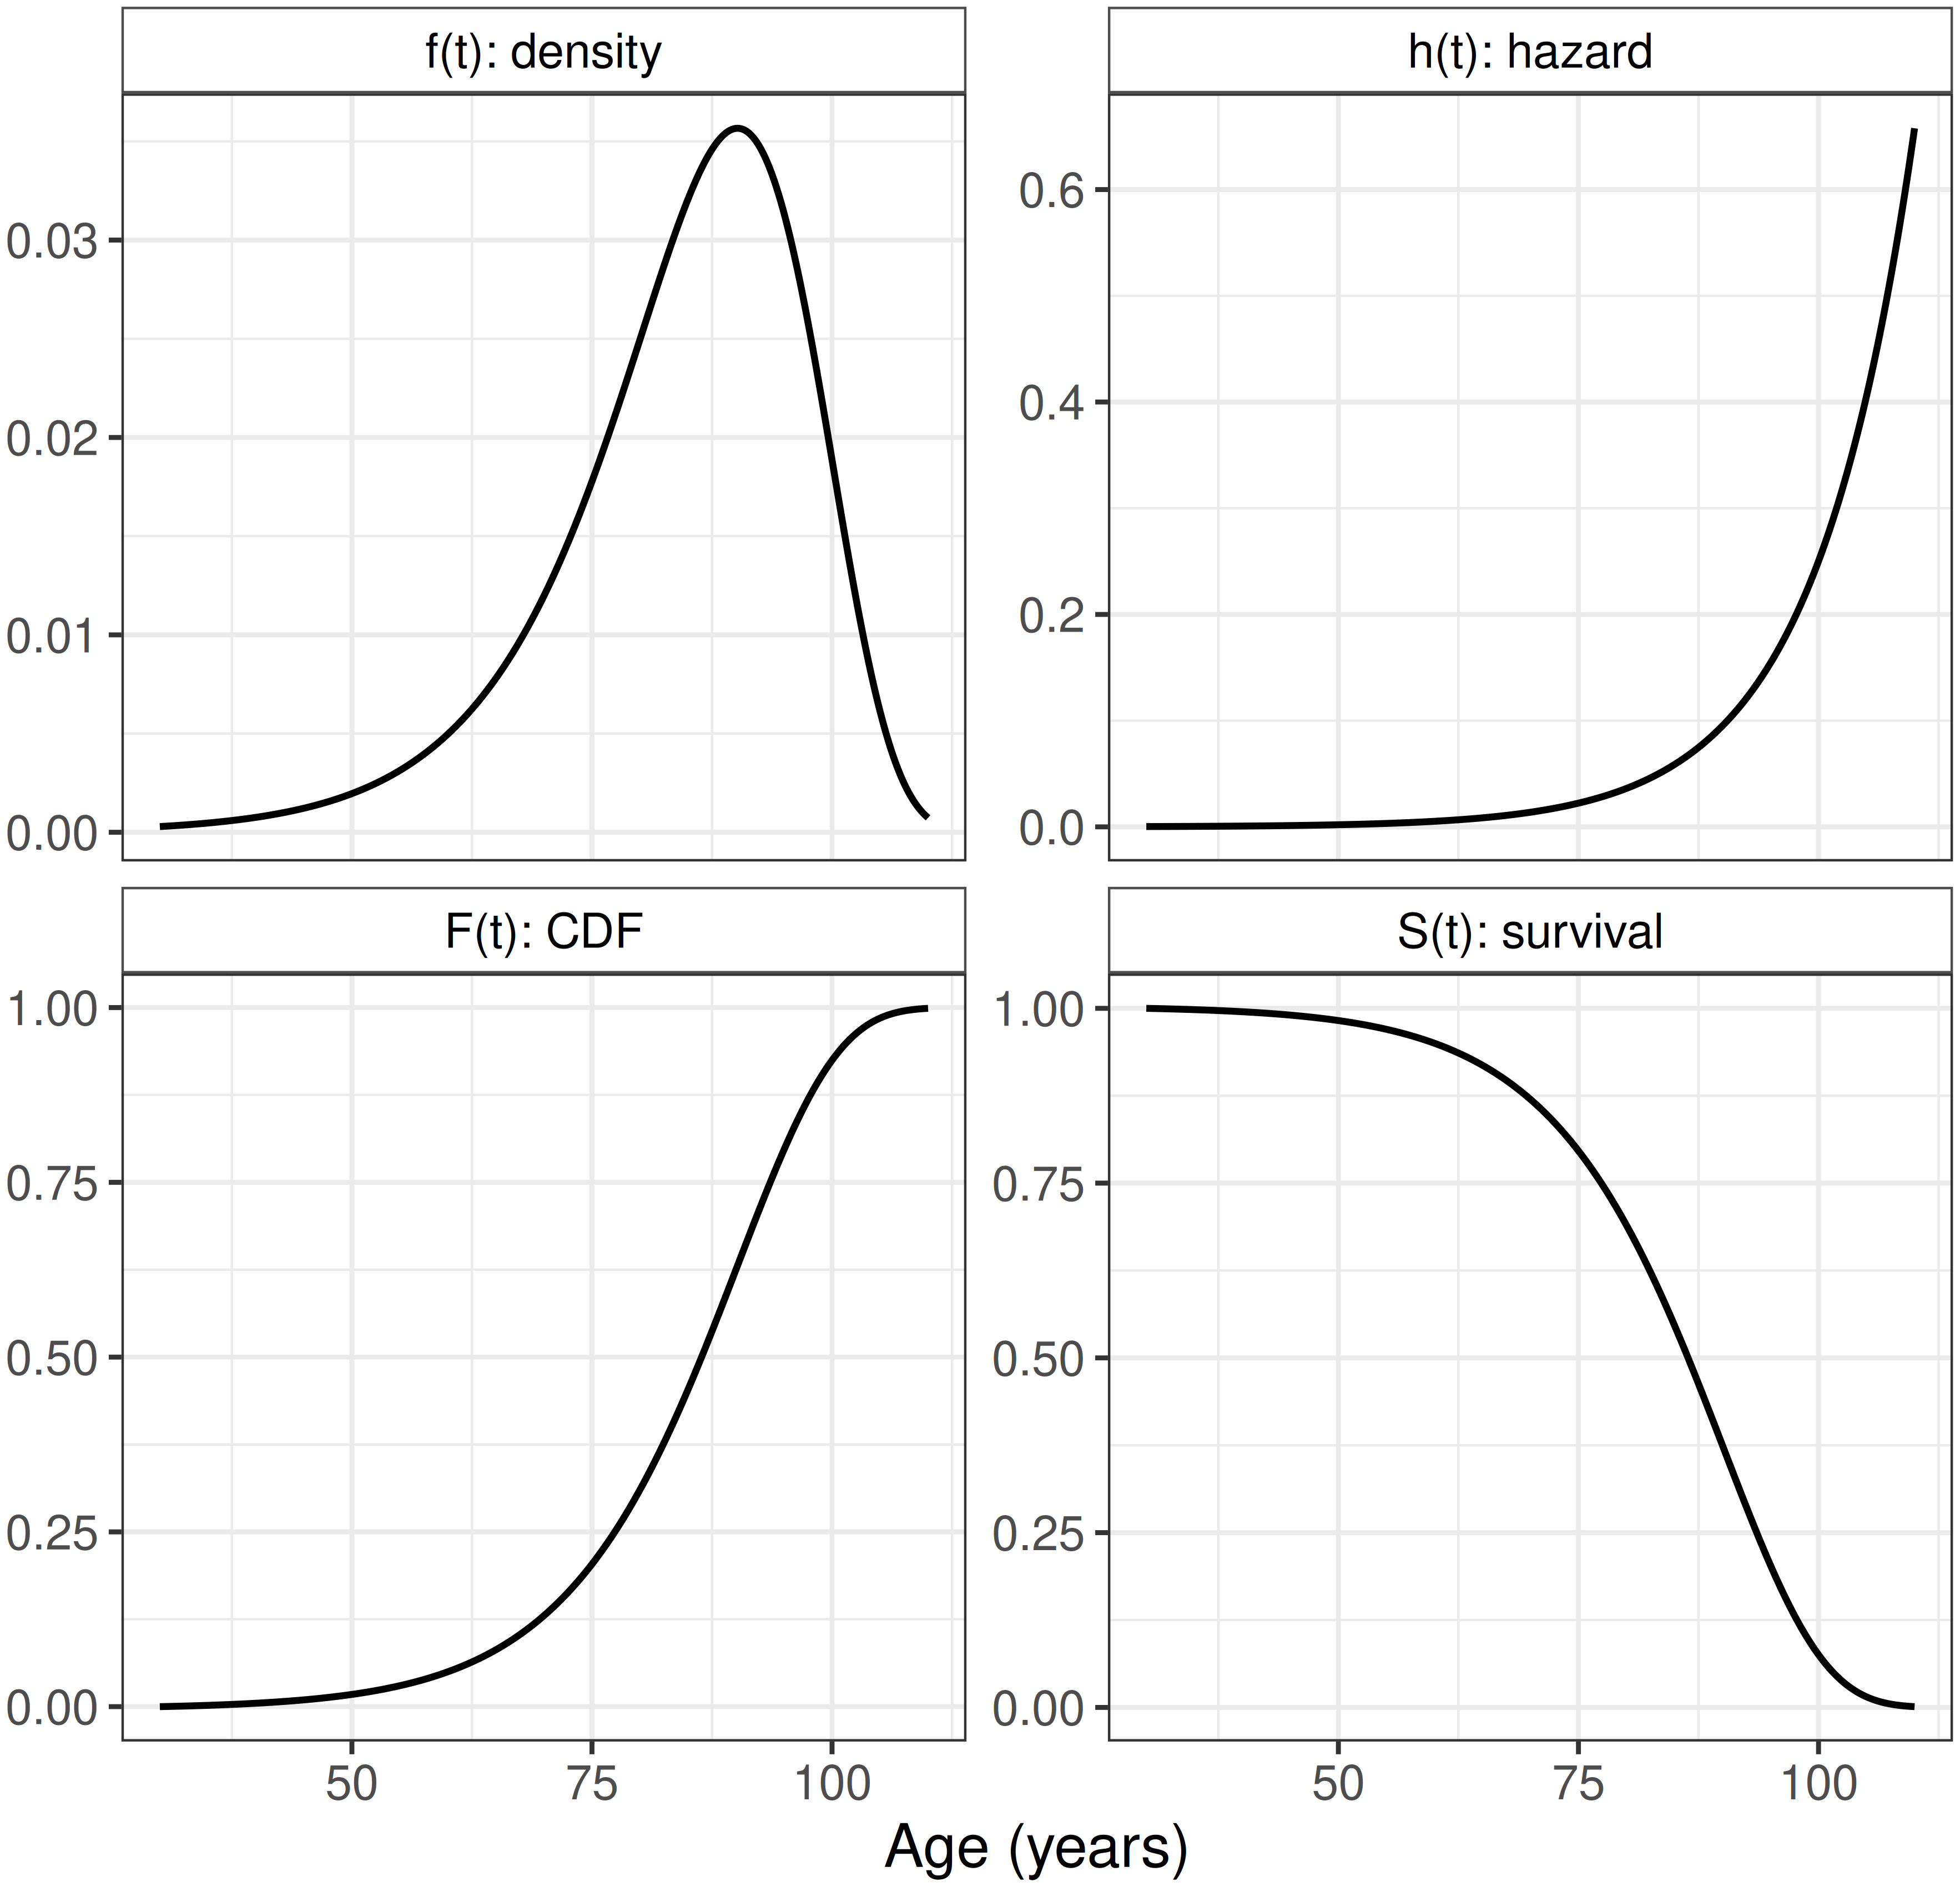
\includegraphics[width=0.8\linewidth,height=\textheight,keepaspectratio]{Figures/introduction/fig-p0c1-gompertz.png}

}

\caption{\label{fig-p0c1-gompertz}Probability density (top left), hazard
(top right), cumulative distribution (bottom left), and survival (bottom
right) functions of a Gompertz distribution with parameters fit to
Swedish age-specific mortality rates for 2019 (sexes combined, ages
30--100). Fitted hazard: \(h(\tau) = a\,e^{b(\tau-30)}\) with
\(a \approx 2.9 \times 10^{-4}\) and \(b \approx 0.097\) per year.}

\end{figure}%

\section{Censoring and truncation}\label{censoring-and-truncation}

As already discussed, censoring\index{censoring} is a defining feature
of survival analysis. In addition to censoring, survival data can
include \emph{truncation}\index{truncation}, which means portions of
follow-up time are excluded. The precise definitions of the different
types of censoring and truncation are provided in
Chapter~\ref{sec-surv}. Brief, non-technical summaries are given below.

The most common form of censoring is
right-censoring\index{censoring!right} (Figure~\ref{fig-p0c1-censoring},
second row), which occurs when the true survival time is greater than
(`to the right of,' if you imagine a number line) the observed censoring
time. The examples in Section~\ref{sec-intro-def} all exhibit forms of
right-censoring. Left-censoring\index{censoring!left} is recorded when
the event of interest is less than (`to the left of') the observed
censoring time. Chapter~\ref{sec-surv} provides an example of someone
telling an interviewer that they started using a phone (the event of
interest) before the interview, but they do not remember when. If the
time-to-event outcome is ``age at first phone use'' then a
\(23\)-year-old who is using a phone but cannot remember when they
started is left-censored at \(23\). Often, the censoring event is
assumed to be independent of the event of interest (for example, random
dropout). However, when the occurrence of another event precludes
observation of the primary event, it is known as a \emph{competing
risk}\index{competing risks} (Chapter~\ref{sec-eha}). For example, if an
unemployed worker is still looking for a job when the study window
closes, the reason for censoring is independent of the
outcome\index{censoring!independent}. In contrast, finding a part-time
job is a competing event as it precludes the primary event (finding
full-time employment) and may depend on the same factors (skills,
availability, local labor market).

\emph{Left-truncation}\index{truncation!left} is the more common form of
truncation and involves data before the truncation time being excluded.
Left-censoring occurs because the event of interest has already
occurred, but the exact time is unknown. Left-truncation happens when
subjects experience the event before meeting the inclusion criteria and
thus never enter the study at all. Truncation affects whether an
individual is included in the observed sample, whereas censoring affects
how much of an included individual's outcome time is observed.

As a concrete example, consider a study on time until death in patients
diagnosed with tuberculosis (TB). Assume enrollment is open to anyone
with a TB diagnosis, including those diagnosed before the study opened.
Left-truncation arises if patients die between their diagnosis and the
study start. These patients are never observed and are absent from the
data, inducing a form of selection bias: the highest-risk cases (those
dying earliest) are systematically missing
(Figure~\ref{fig-p0c1-censoring}, fourth row). Those who do survive to
the study start will enter with a known gap between diagnosis and
enrollment (Figure~\ref{fig-p0c1-censoring}, third row).
Bias\index{selection bias} occurs when delayed entry and the implicit
selection bias are not explicitly accounted for (discussed in full in
Chapter~\ref{sec-surv}).

Another bias that often occurs when time-dependent dynamics of survival
data collection are not explicitly accounted for is \emph{immortal time
bias}\index{immortal time bias}. This occurs when group membership
(treatment) is determined only after a period of guaranteed survival but
is treated as if present from baseline. Immortal time bias is also
discussed further in Chapter~\ref{sec-surv}.

The first part of this book will formally introduce and develop these
concepts further.

\begin{figure}

\centering{

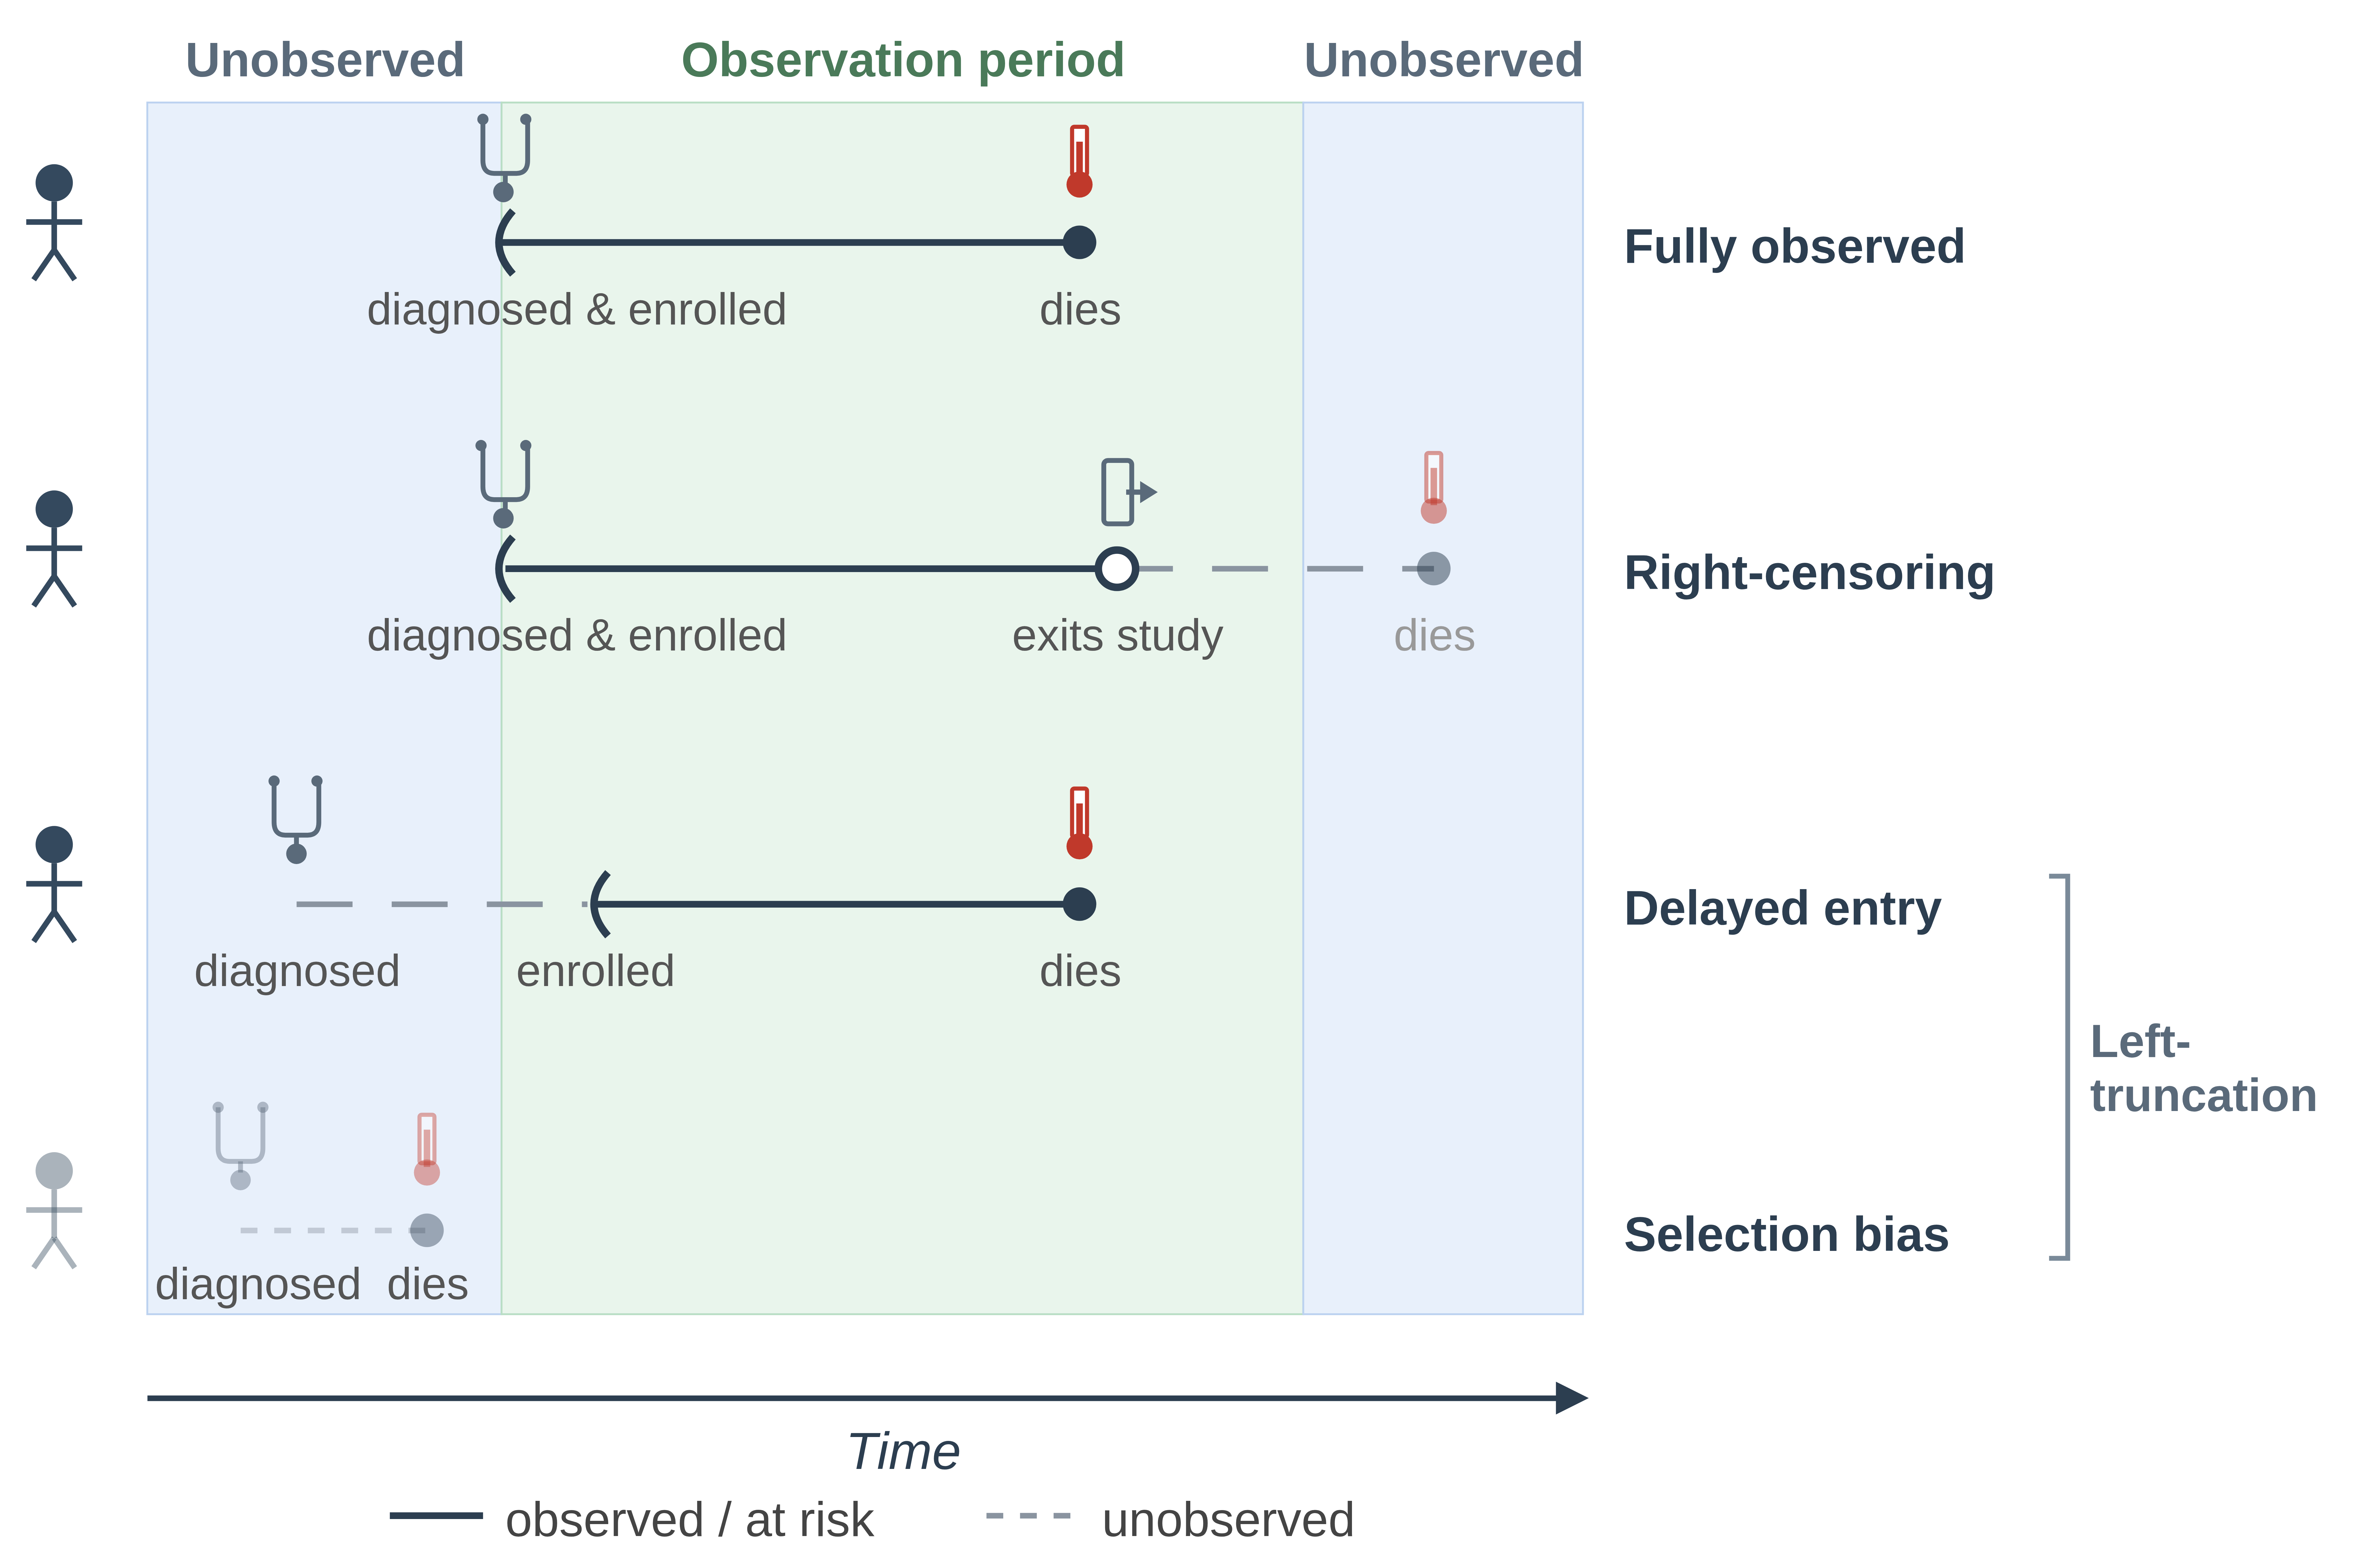
\includegraphics[width=0.9\linewidth,height=\textheight,keepaspectratio]{Figures/introduction/fig-p0c1-censoring.png}

}

\caption{\label{fig-p0c1-censoring}Common forms of censoring and
truncation, shown on a shared time axis where an observation period
(green) is flanked by unobserved periods (blue). Solid lines show time
during which a subject is observed and at risk, dashed lines show
unobserved time, a bracket marks entry into the risk set, filled circles
mark events (deaths), and an open circle marks censoring. First row
(fully observed): a patient is diagnosed and enrolled at the start of
the observation period and is observed to die during the study. Second
row (right-censoring): a patient is diagnosed and enrolled but exits the
study before the event, so their true death occurs later and is
unobserved. Third row (delayed entry): a patient is diagnosed before the
observation period and enrolled only later, so the time between
diagnosis and entry is excluded from the risk set. Fourth row (selection
bias): a patient is diagnosed and dies before the study begins, and so
never enters the sample. Delayed entry and selection bias are both
related to left-truncation.}

\end{figure}%

\part{Machine Learning and Survival Analysis}

\chapter{Machine Learning}\label{sec-ml}

This chapter covers core concepts in machine
learning\index{machine learning}. It is not intended as a general or
comprehensive introduction and does not cover mathematical theory or the
practical implementation of machine learning models in software.
Instead, the purpose is to introduce key concepts and provide basic
intuition for a general machine learning workflow, while also
establishing a shared vocabulary and conceptual framework that will be
used throughout the remainder of the book.

In particular, the focus of this chapter is on machine learning concepts
including tasks\index{machine learning task} (introduced in a survival
context in Chapter~\ref{sec-survtsk}), learners\index{learner}, loss
functions\index{loss function}, resampling\index{resampling}, and
evaluation\index{model evaluation}, which will be essential for
understanding how survival analysis problems can be formulated and
evaluated using machine learning. Many excellent resources (several
freely available) already provide in-depth treatments of machine
learning models and algorithms, and duplication of that material is
deliberately avoided here. References are provided at the end of this
chapter for readers seeking a broader or more technical introduction to
machine learning.

\section{Basic workflow}\label{sec-ml-basics}

This book focuses on \emph{supervised
learning}\index{supervised learning}, in which predictions are made for
outcomes based on data with observed dependent and independent
variables. For example, predicting someone's height is a supervised
learning problem as data can be collected for features (independent
variables) such as age and sex, and the observable outcome (dependent
variable), height. Alternatives to supervised learning include
\emph{unsupervised learning}\index{unsupervised learning},
\emph{semi-supervised learning}\index{semi-supervised learning}, and
\emph{reinforcement learning}\index{reinforcement learning}. This book
is primarily concerned with \emph{predictive} survival analysis, which
means making future predictions based on observed outcomes, a paradigm
that fits naturally within supervised learning\index{model predicting}.

The basic machine learning workflow is represented in
Figure~\ref{fig-p1c3-ml-basic}:

\begin{enumerate}
\def\labelenumi{\arabic{enumi}.}
\tightlist
\item
  Data splitting: Data is split into training and test
  datasets\index{training data}\index{testing data}.
\item
  Training: A learner\index{learner} is selected and is trained on the
  training data, inducing a fitted model.
\item
  Predicting: Features from the test data are passed to the model which
  makes predictions for the unseen outcomes (Box 1).
\item
  Evaluation: Outcomes from the test data are passed to a chosen
  measure\index{performance measure} with the predictions, which
  evaluates the performance\index{model performance} of the model (Box
  2).
\end{enumerate}

The process of (repeatedly) splitting the data into training and test
data is called \emph{resampling}\index{resampling} and running multiple
resampling experiments with different models is called
\emph{benchmarking}\index{benchmarking}. All these concepts will be
explained in this chapter.

\begin{figure}

\centering{

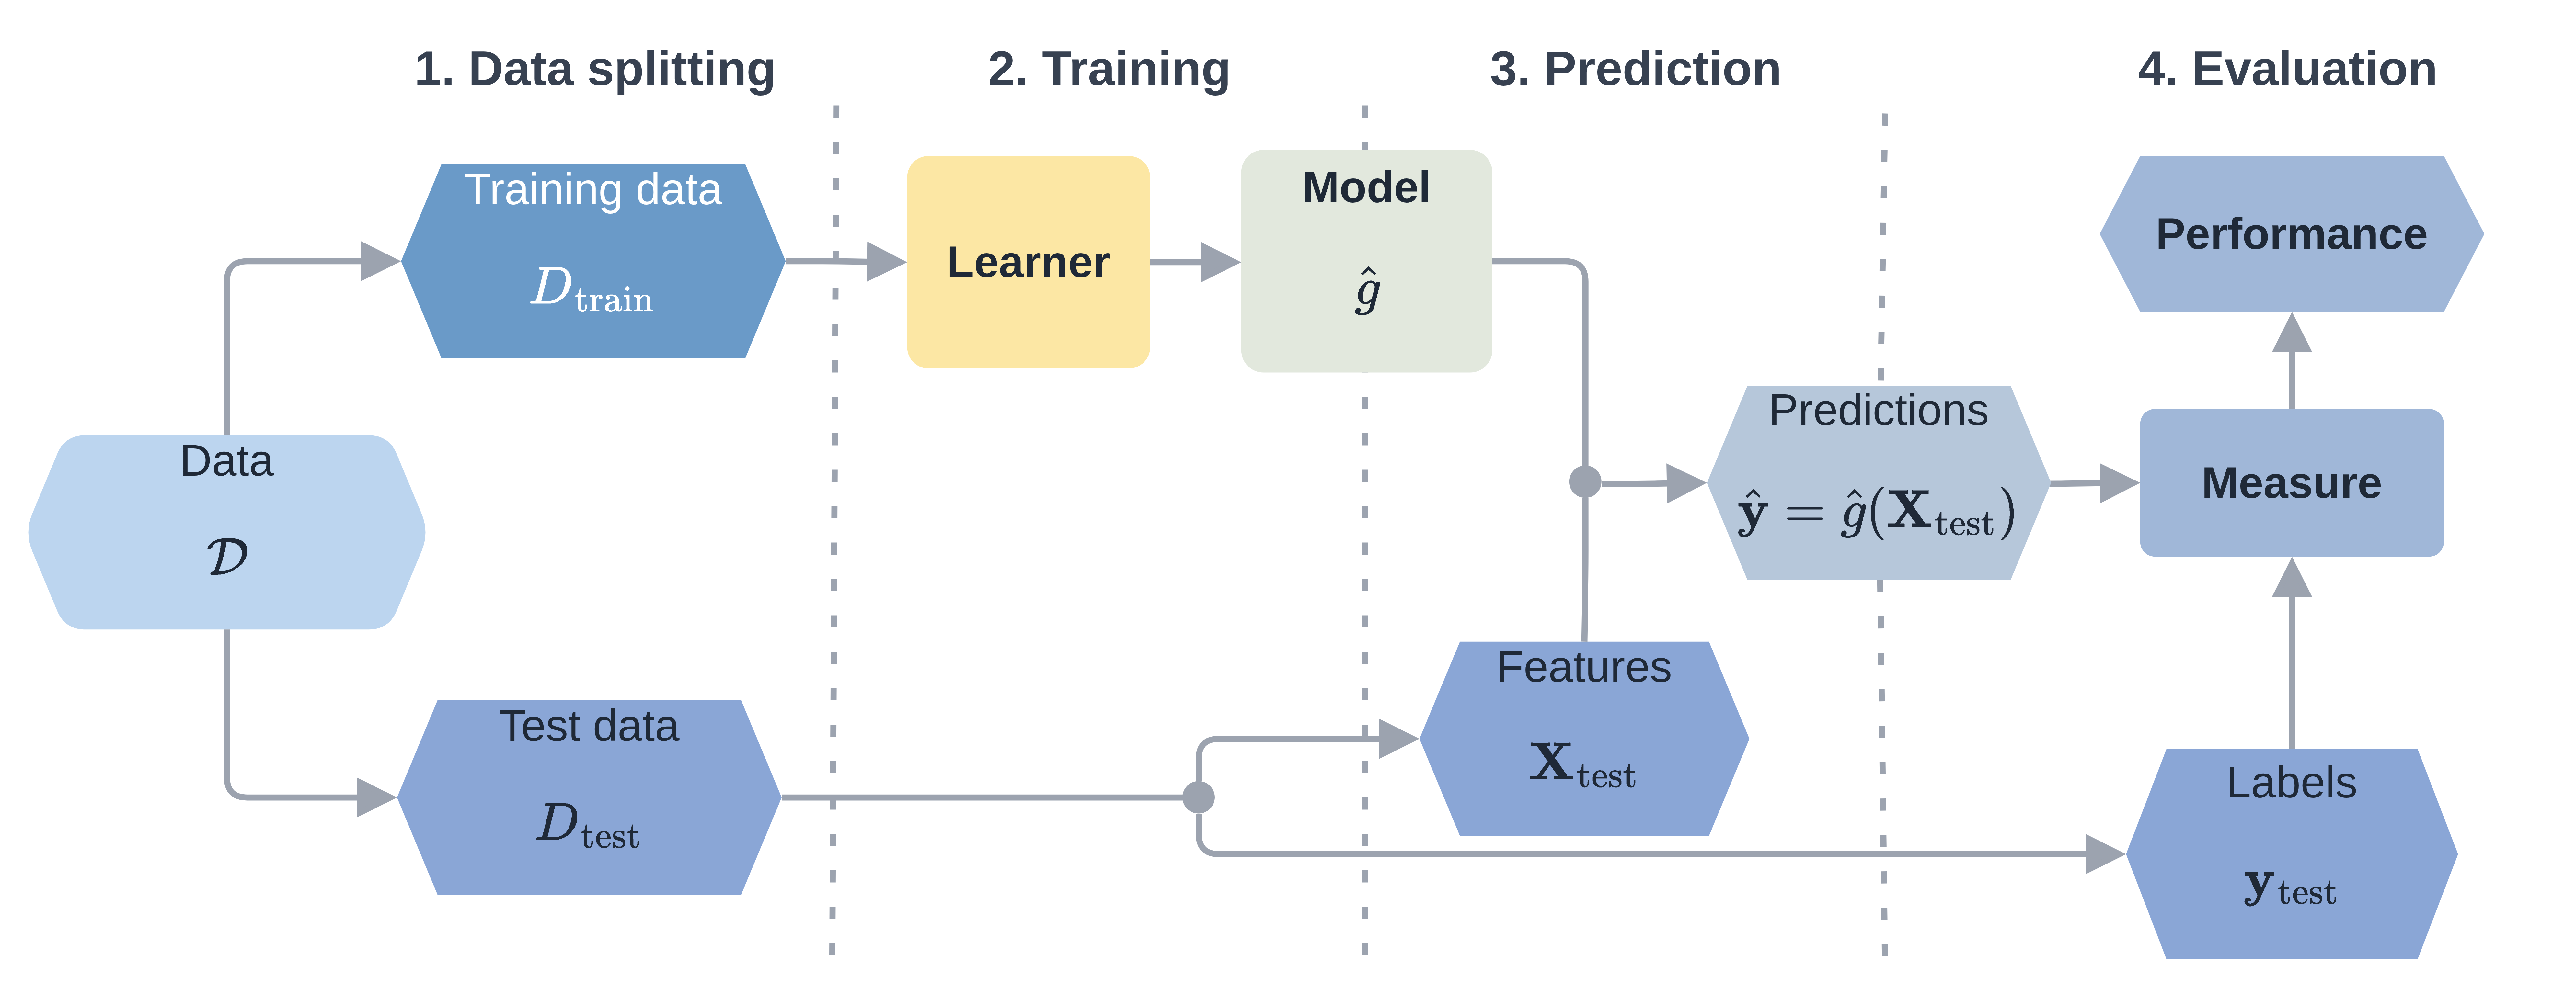
\includegraphics[width=1\linewidth,height=\textheight,keepaspectratio]{Figures/ml/fig-p1c3-ml-basic.png}

}

\caption{\label{fig-p1c3-ml-basic}Basic machine learning workflow. The
available data \(\mathcal{D}\) is split into a training and a test set.
A learner is trained on the training data, inducing a fitted model
\(\hat{g}\); the model is applied to the test features
\(\mathbf{X}_{\textrm{test}}\) to produce predictions
\(\hat{\mathbf{y}}\), which are compared with the test labels
\(\mathbf{y}_{\textrm{test}}\) by a performance measure.}

\end{figure}%

\section{Tasks}\label{sec-ml-tasks}

A machine learning task\index{machine learning task} is the
specification of the mathematical problem that is to be solved by a
given algorithm. Tasks are derived from datasets and one dataset can
give rise to many tasks. For example, a dataset with columns `age',
`weight', `height', `sex', `diagnosis', and `time of death' could give
rise to several supervised tasks:

\begin{itemize}
\tightlist
\item
  Supervised regression\index{regression}: Predict age from weight,
  height, and sex.
\item
  Supervised classification\index{classification}: Predict sex from age
  and diagnosis.
\item
  Supervised survival: Predict time of death from all other features.
\end{itemize}

The specification of a task is vital for interpreting predictions from a
model and its subsequent performance. This is particularly true when
separating between deterministic and probabilistic predictions, as
discussed later in the chapter.

Formally, let \(\mathcal{X}\subseteq \mathbb{R}^p\) be the feature space
for \(p\) features and let \(\mathcal{Y}\) be the target space (or
\emph{outcomes} or \emph{labels}). A dataset is then given by
\(\mathcal{D}= \{(\mathbf{x}_i, y_i)\}_{i=1}^n\) where the observations
are assumed to be independent and identically distributed draws from an
unknown joint distribution.

A machine learning task is the problem of learning the unknown function
\(g : \mathcal{X}\rightarrow \mathcal{Y}\) where \(\mathcal{Y}\)
specifies the nature of the task, for example classification,
regression, or survival. For some tasks, the prediction object may
differ from the outcome space, such as in probabilistic prediction
tasks.

\subsection{Regression}\label{sec-ml-tasks-regr}

Regression tasks make continuous predictions, for example someone's
height.\index{regression} Regression may be
deterministic\index{regression!deterministic}, in which case a single
continuous value is predicted, or
probabilistic\index{regression!probabilistic}, where a probability
distribution over the real numbers is predicted. For example, predicting
an individual's height as 165cm would be a deterministic regression
prediction, whereas predicting their height follows a
\(\mathcal{N}(165, 2^2)\) distribution would be probabilistic.

Formally, a deterministic regression task is specified by
\(g_{Rd} : \mathcal{X}\rightarrow \mathcal{Y}\subseteq \mathbb{R}\), and
a probabilistic regression task by
\(g_{Rp} : \mathcal{X}\rightarrow \mathcal{S}\) where
\(\mathcal{S}\subseteq \operatorname{Distr}(\mathcal{Y})\) and
\(\operatorname{Distr}(\mathcal{Y})\) is the space of distributions over
\(\mathcal{Y}\).

In the machine learning literature, deterministic regression is more
common than probabilistic and hence the shorthand `regression' is used
to refer to deterministic regression.

\subsection{Classification}\label{sec-ml-tasks-classif}

Classification tasks make discrete predictions, for example whether it
will rain, snow, or be sunny tomorrow\index{classification}. Similarly
to regression, predictions may be deterministic or probabilistic.
Deterministic classification\index{classification!deterministic}
predicts which category an observation falls into, whereas probabilistic
classification\index{classification!probabilistic} predicts the
probability of an observation falling into each category. Predicting it
will rain tomorrow is a deterministic prediction whereas predicting
\(\hat{p}(\text{rain}) = 0.6; \hat{p}(\text{snow}) = 0.1; \hat{p}(\text{sunny}) = 0.3\),
is probabilistic.

Formally, a deterministic classification task is given by
\(g_{Cd} : \mathcal{X}\rightarrow \mathcal{Y}\subseteq \mathbb{N}_0\),
and a probabilistic classification task as
\(g_{Cp} : \mathcal{X}\rightarrow [0,1]^k\) where \(k\) is the number of
categories an observation may fall into and the predicted probabilities
should sum to one. In practice, this latter prediction estimates the
conditional class probabilities, \(\Pr(Y = y \mid X = \mathbf{x})\). If
only two categories are possible, these reduce to the \emph{binary
classification} tasks: \(g_{Bd}: \mathcal{X}\rightarrow \{0, 1\}\) and
\(g_{Bp}: \mathcal{X}\rightarrow [0, 1]\) for deterministic and
probabilistic binary classification
respectively\index{classification!binary}.

In the probabilistic binary case it is common to formulate the task to
predict \([0,1]\) not \([0,1]^2\) as the classes are mutually exclusive.
The class for which probabilities are predicted is referred to as the
\emph{positive class}, and the other as the \emph{negative
class}\index{positive class}\index{negative class}.

\section{Training and predicting}\label{sec-ml-models}

The terms \emph{algorithm}, \emph{learner}, and \emph{model} are often
conflated in machine
learning\index{algorithm}\index{learner}\index{model}. A \emph{learner}
is a description of a learning algorithm, prediction algorithm,
parameters, and hyperparameters\index{hyperparameter}. The
\emph{learning algorithm} is a mathematical strategy to estimate the
unknown mapping from features to outcome as represented by a task,
\(g: \mathcal{X}\rightarrow \mathcal{Y}\). During \emph{training}, data,
\(\mathcal{D}\), is fed into the learning algorithm and induces the
\emph{model} \(\hat{g}\). Whereas the learner defines the algorithm for
training and prediction, the model is the result of training the
algorithm on data\index{model training}.

After training the model, a new observation, \(\mathbf{x}_*\), can be
fed to the \emph{prediction algorithm}, which is a mathematical strategy
that uses the model to make a prediction,
\(\hat{y}= \hat{g}(\mathbf{x}_*)\)\index{model predicting}. Algorithms
range in complexity from simple linear equations, with only a few
coefficients to estimate, to complex iterative procedures whose training
and prediction steps differ considerably.

Algorithms usually involve parameters and
hyperparameters\index{hyperparameter}\index{parameter}. Parameters are
learned from data whereas hyperparameters are set beforehand to guide
the algorithms. Model \emph{parameters} (or \emph{weights}),
\(\boldsymbol{\theta}\), are coefficients to be estimated during model
training. Hyperparameters, \(\boldsymbol{\lambda}\), control how the
algorithms are run but are not directly updated by them. Hyperparameters
can be mathematical, for example the learning rate in a gradient
boosting machine\index{gradient boosting machines}
(Chapter~\ref{sec-boost}), or structural, for example the depth of a
decision tree\index{decision tree} (Chapter~\ref{sec-ranfor}) or the
architecture of a neural network\index{neural networks}
(Chapter~\ref{sec-nnet}). The number of hyperparameters usually
increases with learner complexity and affects its predictive
performance. Often hyperparameters need to be
tuned\index{hyperparameter optimization} (Section~\ref{sec-ml-opt})
instead of manually set.

An example bringing these concepts together is given in Box 1.

\begin{tcolorbox}[enhanced jigsaw, toprule=.15mm, bottomtitle=1mm, opacityback=0, breakable, leftrule=.75mm, title={Box 1 (Ridge regression)}, toptitle=1mm, bottomrule=.15mm, colback=white, colframe=quarto-callout-note-color-frame, titlerule=0mm, opacitybacktitle=0.6, coltitle=black, rightrule=.15mm, left=2mm, colbacktitle=quarto-callout-note-color!10!white, arc=.35mm]

Let \(g : \mathcal{X}\rightarrow \mathcal{Y}\) be the
regression\index{regression} task of interest with
\(\mathcal{X}\subseteq \mathbb{R}\) (a single feature) and
\(\mathcal{Y}\subseteq \mathbb{R}\). Let
\(\boldsymbol{\mathbf{x}} = ({x}_1 \ {x}_2 \cdots {x}_{n})^\top\) and
\(\boldsymbol{\mathbf{y}} = ({y}_1 \ {y}_2 \cdots {y}_{n})^\top\) be
data such that \(x_i \in \mathcal{X}\) and \(y_i \in \mathcal{Y}\) for
all \(i = 1,\ldots,n\).

Say the learner of interest is a regularized linear regression
model\index{linear regression} with learning algorithm:

\[
(\hat{\beta}_0,\hat{\beta}_1):=\mathop{\mathrm{arg\,min}}_{\beta_0,\beta_1}\left(\sum_{i=1}^n\left(y_i-\beta_0 -\beta_1 x_i\right)^2+\gamma\beta_1^2\right).
\]

and prediction algorithm:

\[
\hat{g}(x):= g(x \mid \hat{\boldsymbol{\theta}}) = \hat{\beta}_0 + \hat{\beta}_1 x
\]

The hyperparameter\index{hyperparameter} vector is
\(\boldsymbol{\lambda}= (\gamma) \in \mathbb{R}_{>0}\) and the
parameters are \(\boldsymbol{\theta}= (\beta_0 \ \beta_1)^\top\). Say
that \(\gamma = 2\) is set and the learner is then trained by passing
\((\mathbf{x}, \mathbf{y})\) to the learning algorithm and thus
estimating \(\hat{\boldsymbol{\theta}}\). A prediction, \(\hat{y}\), can
then be made by passing new data \(x_* \in \mathcal{X}\) to the fitted
model,

\[
\hat{y}:= \hat{g}(x_*) = \hat{\beta}_0 + \hat{\beta}_1x_*.
\]

\end{tcolorbox}

\section{Evaluating and benchmarking}\label{sec-ml-eval}

A central component of machine learning best practice is rigorous,
empirical model evaluation\index{model evaluation}. Building a complex
model does not guarantee strong predictive performance. Moreover,
testing performance on a single dataset only provides limited insight
into how a model will generalize to new data. This issue is especially
pronounced in modern pre-trained generative AI
models\index{artificial intelligence!generative}, where there is often
an implicit assumption by users that these models will perform well
across a wide range of domains without task-specific validation.
Trusting a model's performance requires two elements: firstly,
quantifying performance using appropriate and interpretable
measures\index{performance measure}; secondly, clearly specifying what
exactly is being assessed and how.

\subsection{Evaluation}\label{sec-ml-evaluation}

To understand whether a model is `good', its predictions are evaluated
with a \emph{loss
function}\index{loss function}\index{model evaluation}. In general,
losses compare an observed outcome with a prediction object, which could
be a numeric value, a class probability vector, or a predicted
distribution. For deterministic predictions, loss functions assign a
score to the discrepancy between predictions and true values,
\(L: \mathcal{Y}\times \mathcal{Y}\rightarrow \bar{\mathbb{R}}\). This
formulation is general and also covers losses that can take negative or
infinite values, such as those based on the negative log-likelihood. In
practice, many losses are non-negative, such as the \emph{absolute
loss},
\(L(y, \hat{y}) = \vert y - \hat{y} \vert\)\index{absolute error}.

A model is considered truly useful if it performs well \emph{in
general}, meaning it should perform well on new, previously unseen data,
rather than only the data encountered during training and development. A
model's \emph{generalization error}\index{generalization error} refers
to its expected performance on new data. Given some loss \(L\), a
trained model \(\hat{g}\), and random data \((X, Y)\), then the
generalization error is the expectation of the loss over an independent
test sample, \(\mathbb{E}[L(Y, \hat{g}(X))]\).

A model should only be used to make predictions if its generalization
error is estimated to be acceptable for a given context. If a model were
trained and evaluated on the same data, the resulting loss, known as the
\emph{training error}\index{training error}, would be an overoptimistic
estimate of the true generalization error (James et al. 2013). This
occurs because the model is making predictions for data it has already
`seen' and therefore the loss does not evaluate the model's ability to
generalize to new, unseen data. Estimation of the generalization error
requires \emph{data splitting}\index{data splitting}, which is the
process of splitting available data, \(\mathcal{D}\), into
\emph{training data}\index{training data},
\(\mathcal{D}_{train}\subset \mathcal{D}\), and \emph{testing
data}\index{testing data},
\(\mathcal{D}_{test}= \mathcal{D}\setminus \mathcal{D}_{train}\).
Another benefit of data splitting is to help detect model
overfitting\index{overfitting}, which occurs when models learn patterns
specific to the training data that do not generalize to new data.
Overfitting can be mitigated through methods that constrain model
complexity and reduce the tendency to fit noise in the training data;
examples include feature selection\index{feature selection},
penalization\index{penalization} methods, and early
stopping\index{early stopping}.

\subsection{Resampling and benchmarking}\label{sec-ml-resampling}

The simplest method to estimate the generalization error is
\emph{holdout resampling}\index{resampling!holdout}, which is the
process of partitioning the data into one training dataset and one
testing dataset, with the model trained on the former and predictions
made for the latter. Using 2/3 of the data for training and 1/3 for
testing is a common splitting ratio (Kohavi 1995). Splitting the data
randomly ensures that potential patterns or information encoded in the
ordering of the data are removed; these patterns are unlikely to
generalize to new, unseen data. For example, in clinical datasets, the
order in which patients enter a study might inadvertently encode latent
information such as which doctor was on duty at the time, which could
theoretically influence patient outcomes. As this information is not
explicitly captured in measured features, it is unlikely to hold
predictive value for future patients. Random splitting breaks any
spurious associations between the order of data and the outcomes.

Holdout resampling is a quick method to estimate the generalization
error, and is particularly useful when very large datasets are
available. However, holdout resampling has a very high variance for
small datasets and there is no guarantee that evaluating the model on
one holdout split is indicative of real-world performance.

\(k\)-fold cross-validation (CV)\index{resampling!cross-validation} can
be used as a more robust method to estimate the generalization
error\index{generalization error} (Hastie, Tibshirani, and Friedman
2001). \(k\)-fold CV partitions the data into \(k\) subsets, called
\emph{folds}. The training data consists of \(k-1\) of the folds and the
remaining one is used for testing and evaluation. This is repeated \(k\)
times until each of the folds has been used exactly once as the testing
data. The performance from each fold is averaged into a final
performance estimate (Figure~\ref{fig-p1c3-cv}). It is common to use
\(k = 5\) or \(k = 10\) (Leo Breiman and Spector 1992; Kohavi 1995).
This process can be repeated multiple times (\emph{repeated \(k\)-fold
CV})\index{resampling!cross-validation} and/or \(k\) can even be set to
\(n\), which is known as \emph{leave-one-out cross-validation}.

Cross-validation can also be stratified, which ensures that a variable
of interest will have the same distribution in each fold as in the
original data\index{resampling!stratified cross-validation}. This is
important, and often recommended, in survival analysis to ensure that
the proportion of censoring\index{censoring} in each fold is
representative of the full dataset (Casalicchio and Burk 2024; Herrmann
et al. 2021). Other resampling mechanisms may also be useful for event
history analysis\index{event history analysis} (Chapter~\ref{sec-eha}).
For example, stratifying with respect to different competing
risks\index{competing risks}, or using more complex resampling schemes
that can handle non-independent observations for recurrent
events\index{recurrent events} data (Hornung et al. 2023).

\begin{figure}

\centering{

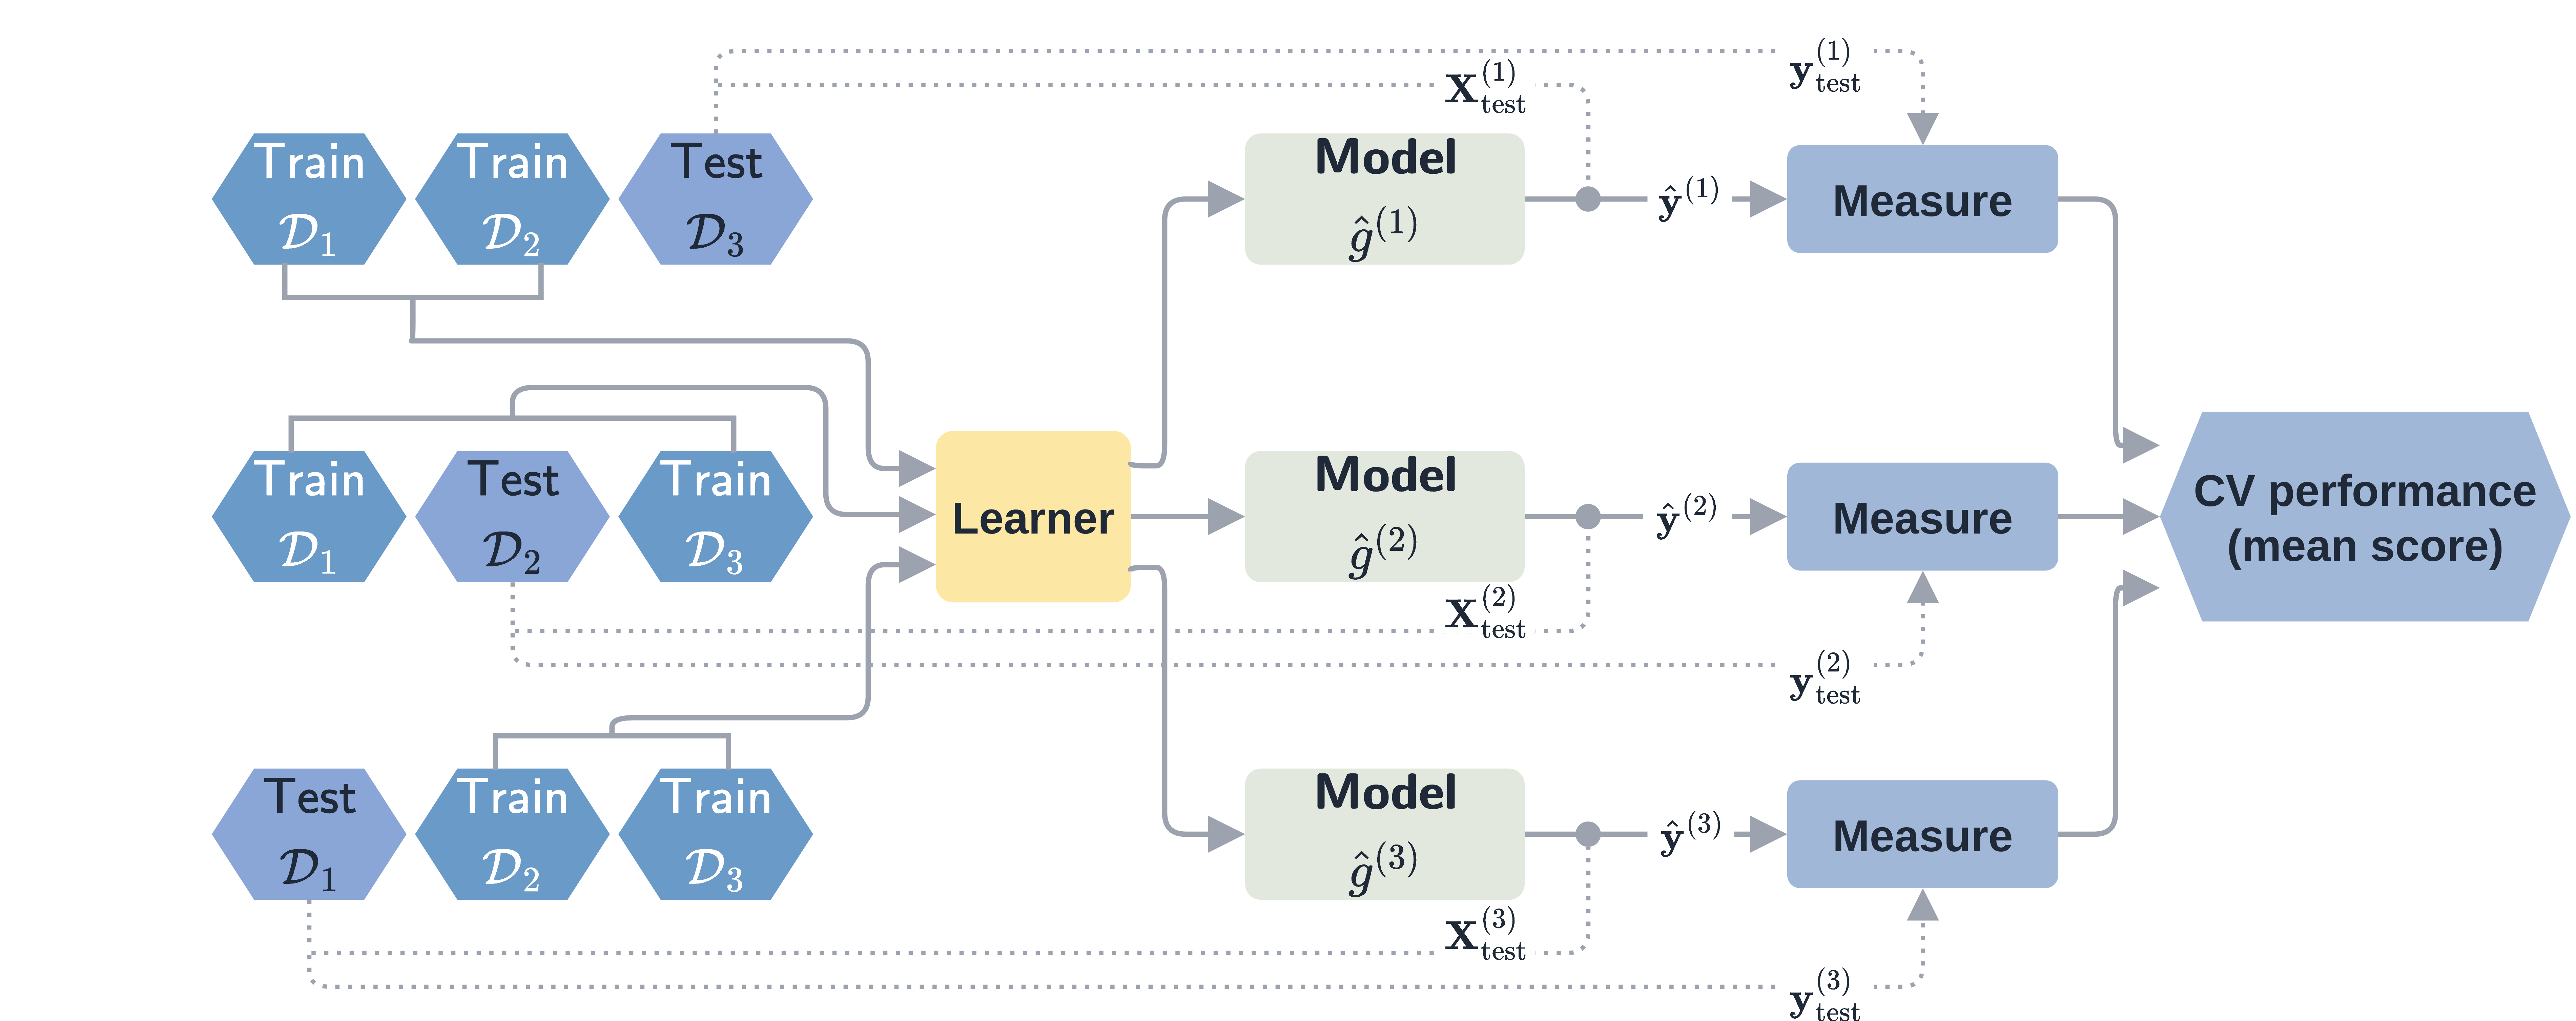
\includegraphics[width=1\linewidth,height=\textheight,keepaspectratio]{Figures/ml/fig-p1c3-cv.png}

}

\caption{\label{fig-p1c3-cv}Three-fold cross-validation. The data is
partitioned into three folds; across the three iterations each fold is
held out once for testing (highlighted) while the remaining two folds
are used for training. The same learner is trained on every fold's
training data, yielding a fold-specific model \(\hat{g}^{(k)}\) that is
evaluated on the held-out fold via a performance measure. The three
per-fold measures are averaged into a single cross-validation
performance estimate.}

\end{figure}%

Repeating resampling experiments with multiple models is referred to as
a \emph{benchmark experiment}\index{benchmarking}. A benchmark
experiment compares models by evaluating their performance on
\emph{identical} data, which means the same resampling\index{resampling}
strategy and folds should be used for all models. Determining if one
model performs better than another is a surprisingly complex topic
(Benavoli et al. 2017; Demšar 2006; Dietterich 1998; Nadeau and Bengio
2003; Schulz-Kümpel et al. 2025) and is out of scope for this book. A
common heuristic is to suggest one model outperforms another if it
consistently performs better across the majority of folds in a repeated
cross-validation benchmark experiment. However, this is just a heuristic
and without robust hypothesis testing results should be interpreted with
caution.

\begin{tcolorbox}[enhanced jigsaw, toprule=.15mm, bottomtitle=1mm, opacityback=0, breakable, leftrule=.75mm, title={Box 2 (Evaluating ridge regression)}, toptitle=1mm, bottomrule=.15mm, colback=white, colframe=quarto-callout-note-color-frame, titlerule=0mm, opacitybacktitle=0.6, coltitle=black, rightrule=.15mm, left=2mm, colbacktitle=quarto-callout-note-color!10!white, arc=.35mm]

Let \(\{(x_i, y_i)\}^m_{i=1}\) be data previously unseen by the model
trained in Box 1. Predictions are made by passing the new data to the
fitted model,

\[
\hat{y}_i := \hat{g}(x_i) = \hat{\beta}_0 + \hat{\beta}_1x_i, \quad i = 1,\ldots,m.
\]

The model's predictive performance can then be evaluated, for example
with the mean absolute error,

\[
L(\mathbf{y}, \hat{\mathbf{y}}) = \frac{1}{m} \sum^{m}_{i = 1} \vert y_i - \hat{y}_i \vert,
\]

where \(\boldsymbol{\mathbf{y}} = ({y}_1 \ {y}_2 \cdots {y}_{m})^\top\)
and
\(\boldsymbol{\mathbf{\hat{y}}} = ({\hat{y}}_1 \ {\hat{y}}_2 \cdots {\hat{y}}_{m})^\top\)
are the vectors of observed and predicted values respectively.

\end{tcolorbox}

\section{Hyperparameter optimization}\label{sec-ml-opt}

Section~\ref{sec-ml-models} introduced model
hyperparameters\index{hyperparameter}, which control how training and
prediction algorithms are run. Setting hyperparameters is a critical
part of model fitting and can significantly change model performance.
\emph{Tuning}\index{hyperparameter optimization} is the process of using
internal benchmark experiments to automatically select the optimal
hyperparameter configuration. For example, the regularization parameter,
\(\gamma\), in ridge regression\index{ridge} is a potential
hyperparameter to tune. This hyperparameter may be tuned over a range of
values, say \([0.1, 25]\), or over a discrete subset, for example
\(\{0.1, 10, 25\}\). Using the discrete example, tuning the
regularization parameter would effectively involve comparing three
independent ridge regression models in a benchmark experiment with
\(\gamma=0.1\), \(\gamma=10\), and \(\gamma=25\) respectively. The value
of \(\gamma\) that results in the model with the optimal performance is
then selected for the hyperparameter value going forward. \emph{Nested
resampling}\index{resampling!nested} is a method to reduce bias that
could occur from using overlapping data for tuning, training, or testing
(R. Simon 2007). Nested resampling is the process of resampling the
training set again for tuning before then refitting the optimal model on
the entire training data.

\section{Parameter optimization}\label{parameter-optimization}

Many machine learning models, including gradient boosting
machines\index{gradient boosting machines} (Chapter~\ref{sec-boost}) and
neural networks\index{neural networks} (Chapter~\ref{sec-nnet}), depend
on iteration to fit parameters to the training data.\index{iteration}
This section briefly covers a common technique for iterative parameter
optimization using gradient descent
(Section~\ref{sec-ml-gradient-descent}) and then a process for
controlling the number of iterations known as early stopping
(Section~\ref{sec-ml-early-stopping}).

\subsection{Gradient descent}\label{sec-ml-gradient-descent}

Many machine learning algorithms use \emph{gradient
descent}\index{gradient descent} to estimate the model parameters,
\(\boldsymbol{\theta}\), during training. Gradient descent is commonly
used when no closed-form solution exists for minimizing a loss function.
Given a differentiable loss function, \(L(\boldsymbol{\theta})\), that
measures how well the model predicts the training data, gradient descent
repeatedly updates the parameter estimates by taking small steps that
decrease the loss until the loss stabilizes or a stopping criterion is
met. This principle is central to neural networks\index{neural networks}
(Chapter~\ref{sec-nnet}) and is closely related to the functional
gradient view of gradient boosting\index{gradient boosting machines}
(Chapter~\ref{sec-boost}), but is easier to introduce for a simple
linear regression model\index{linear regression} with only two
parameters.

Consider the linear regression model
\(y = g(x \mid \boldsymbol{\theta}) = \beta_0 + \beta_1 x\) with
parameter vector \(\boldsymbol{\theta}= (\beta_0 \ \beta_1)^\top\),
fitted to observations \(\{(x_i, y_i)\}^n_{i=1}\) by minimizing the
\emph{mean squared error}\index{mean squared error} loss:

\begin{equation}\phantomsection\label{eq-ml-mse}{
L(\boldsymbol{\theta}) = \frac{1}{n}\sum_{i=1}^n \bigl(y_i - \beta_0 - \beta_1 x_i\bigr)^2.
}\end{equation}

The \emph{gradient} of this loss is the vector of partial derivatives of
the loss with respect to each parameter:

\[
\nabla_{\boldsymbol{\theta}} L = \bigl(\partial L / \partial \beta_0 \ \partial L / \partial \beta_1\bigr)^\top.
\]

For any parameter values \(\boldsymbol{\theta}\), the gradient describes
how the loss changes when the parameters are changed. If the gradient
component for a parameter is positive, decreasing that parameter reduces
the loss; if negative, increasing the parameter reduces the loss.
Gradient descent therefore updates the parameters in the \emph{opposite}
direction of the gradient to reduce the loss,
\begin{equation}\phantomsection\label{eq-ml-gd}{
\boldsymbol{\theta}^{t+1} = \boldsymbol{\theta}^{t} - \alpha \,\nabla_{\boldsymbol{\theta}} L\bigl(\boldsymbol{\theta}^{t}\bigr),
}\end{equation}

where \(\alpha > 0\) is the \emph{learning rate},\index{learning rate}
also known as the step size, as it controls the size of the parameter
update at each iteration. If \(\alpha\) is too small, then convergence
is slow, but if it is too large, iterations can overshoot or oscillate.
In machine learning models \(\alpha\) is typically
tuned\index{hyperparameter optimization} (Section~\ref{sec-ml-opt}) or
adaptive and combined with early stopping\index{early stopping}
(Section~\ref{sec-ml-early-stopping}).

Starting from an arbitrary initial guess \(\boldsymbol{\theta}^{0}\),
(\ref{eq-ml-gd}) is repeated to drive \(\boldsymbol{\theta}\) towards a
minimum of \(L\).

For the loss in (\ref{eq-ml-mse}), the partial derivatives are:
\begin{equation}\phantomsection\label{eq-mse-partials}{
\begin{aligned}
\frac{\partial L}{\partial \beta_0} &= -\frac{2}{n}\sum_{i=1}^n (y_i - \beta_0 - \beta_1 x_i), \\
\frac{\partial L}{\partial \beta_1} &= -\frac{2}{n}\sum_{i=1}^n x_i (y_i - \beta_0 - \beta_1 x_i).
\end{aligned}
}\end{equation}

In a simple example, suppose the data are \(\{(3, 1.8), (2, 14)\}\), the
initial guess is \(\boldsymbol{\theta}^{0} = (1 \ 1)^\top\), and
\(\alpha=0.1\), then substituting (\ref{eq-mse-partials}) into
(\ref{eq-ml-gd}) gives:

\[
\begin{aligned}
\boldsymbol{\theta}^1 &= 
\begin{pmatrix}
1 \\
1 \\
\end{pmatrix} - 0.1
\begin{pmatrix}
-\frac{2}{n}\sum_{i=1}^n (y_i - 1 - x_i) \\
-\frac{2}{n}\sum_{i=1}^n x_i (y_i - 1 - x_i) \\
\end{pmatrix} \\
&=
\begin{pmatrix}
1 \\
1 \\
\end{pmatrix} - 0.1
\begin{pmatrix}
-\frac{2}{2}((1.8 - 1 - 3) + (14 - 1 - 2)) \\
-\frac{2}{2}(3(1.8 - 1 - 3) + 2(14 - 1 - 2)) \\
\end{pmatrix} \\
&=
\begin{pmatrix}
1 \\
1 \\
\end{pmatrix} - 0.1
\begin{pmatrix}
-8.8 \\
-15.4 \\
\end{pmatrix} =
\begin{pmatrix}
1.88 \\
2.54 \\
\end{pmatrix}.
\end{aligned}
\]

As can be seen, each gradient-descent step updates all parameters
simultaneously.

Linear regression minimized by the mean squared error has a known,
closed-form solution (ordinary least squares).
Figure~\ref{fig-p1c3-gradient-descent} illustrates gradient descent for
an example with more observations, comparing the gradient descent
procedure to the known closed-form optimum. The contours show the loss
surface of \(L(\boldsymbol{\theta})\) over the two-dimensional parameter
space; lighter colors correspond to a smaller loss. Starting from a
deliberately poor initial guess (green square), gradient descent traces
the blue path along the loss surface and finishes (red circle) at the
known closed-form optimum (black cross). At every step, the update moves
in the direction \(-\nabla_{\boldsymbol{\theta}} L\); as the gradient
becomes smaller near the optimum, the parameter updates also become
smaller.

\begin{figure}

\centering{

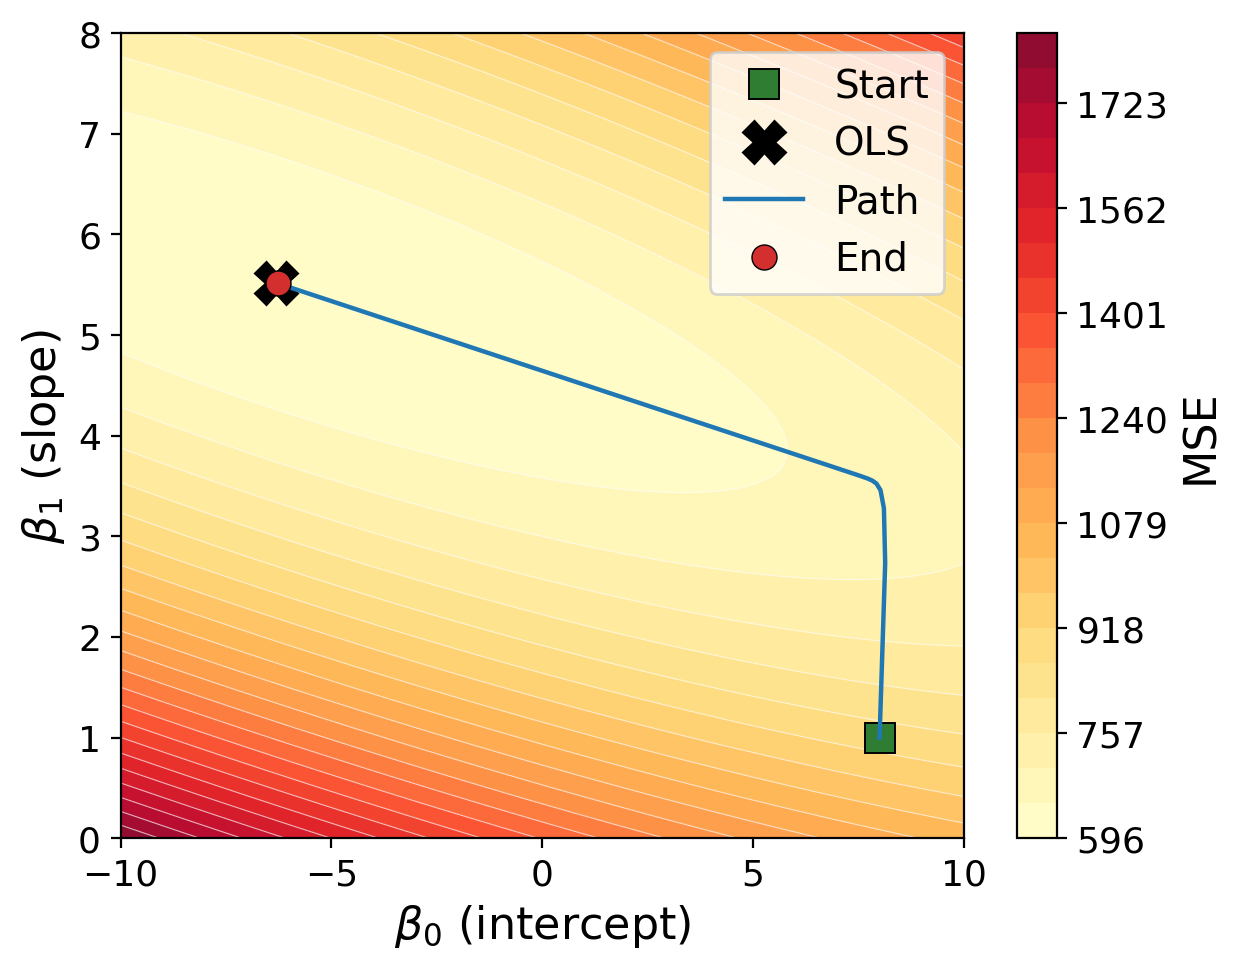
\includegraphics[width=0.7\linewidth,height=\textheight,keepaspectratio]{Figures/ml/fig-p1c3-gradient-descent.png}

}

\caption{\label{fig-p1c3-gradient-descent}Gradient descent on a
two-parameter linear regression problem. Contours and color show the
mean squared error loss \(L(\boldsymbol{\theta})\) from
(\ref{eq-ml-mse}) in the parameter space \((\beta_0 \ \beta_1)^\top\).
The black cross marks the closed-form ordinary least squares optimum.
From the start point (green square), gradient descent follows the blue
path of (\ref{eq-ml-gd}), ending close to the optimum (red circle).}

\end{figure}%

Adaptations to gradient descent, including stochastic gradient descent
and mini-batching, are discussed in Section~\ref{sec-nn-batches}.

\subsection{Early stopping}\label{sec-ml-early-stopping}

Iterative optimization introduces a practical question: how many
iterations should be used? Continuing training for too long can lead to
overfitting\index{overfitting} in which the model starts to capture
noise specific to the training data and generalizes poorly to new
observations. The number of iterations is therefore a hyperparameter
controlling model complexity. Instead of tuning this hyperparameter, a
common technique is to use \emph{early stopping}\index{early stopping}.

Early stopping monitors predictive performance on a held-out validation
set (Section~\ref{sec-ml-resampling}) as training proceeds. This
validation set is typically a subset of the training dataset, meaning
that it is common for a dataset \(\mathcal{D}\) to be split into
\(\mathcal{D}_{train}\) for training the model,
\(\mathcal{D}_{validation}\) for monitoring performance \emph{during}
training, and \(\mathcal{D}_{test}\) for evaluating performance
\emph{after} training. These datasets can be created using any of the
resampling methods in Section~\ref{sec-ml-resampling}. As discussed in
Section~\ref{sec-ml-evaluation}, evaluating a model on the training data
results in overoptimistic estimates of the true generalization error. As
the number of iterations increases, the training error decreases
steadily, whereas the validation error typically decreases at first and
then begins to increase once the model starts to overfit.
Figure~\ref{fig-p1c3-early-stopping} illustrates this on the
gradient-descent example of Section~\ref{sec-ml-gradient-descent}, using
part of the data for training and the remainder for validation.

\begin{figure}

\centering{

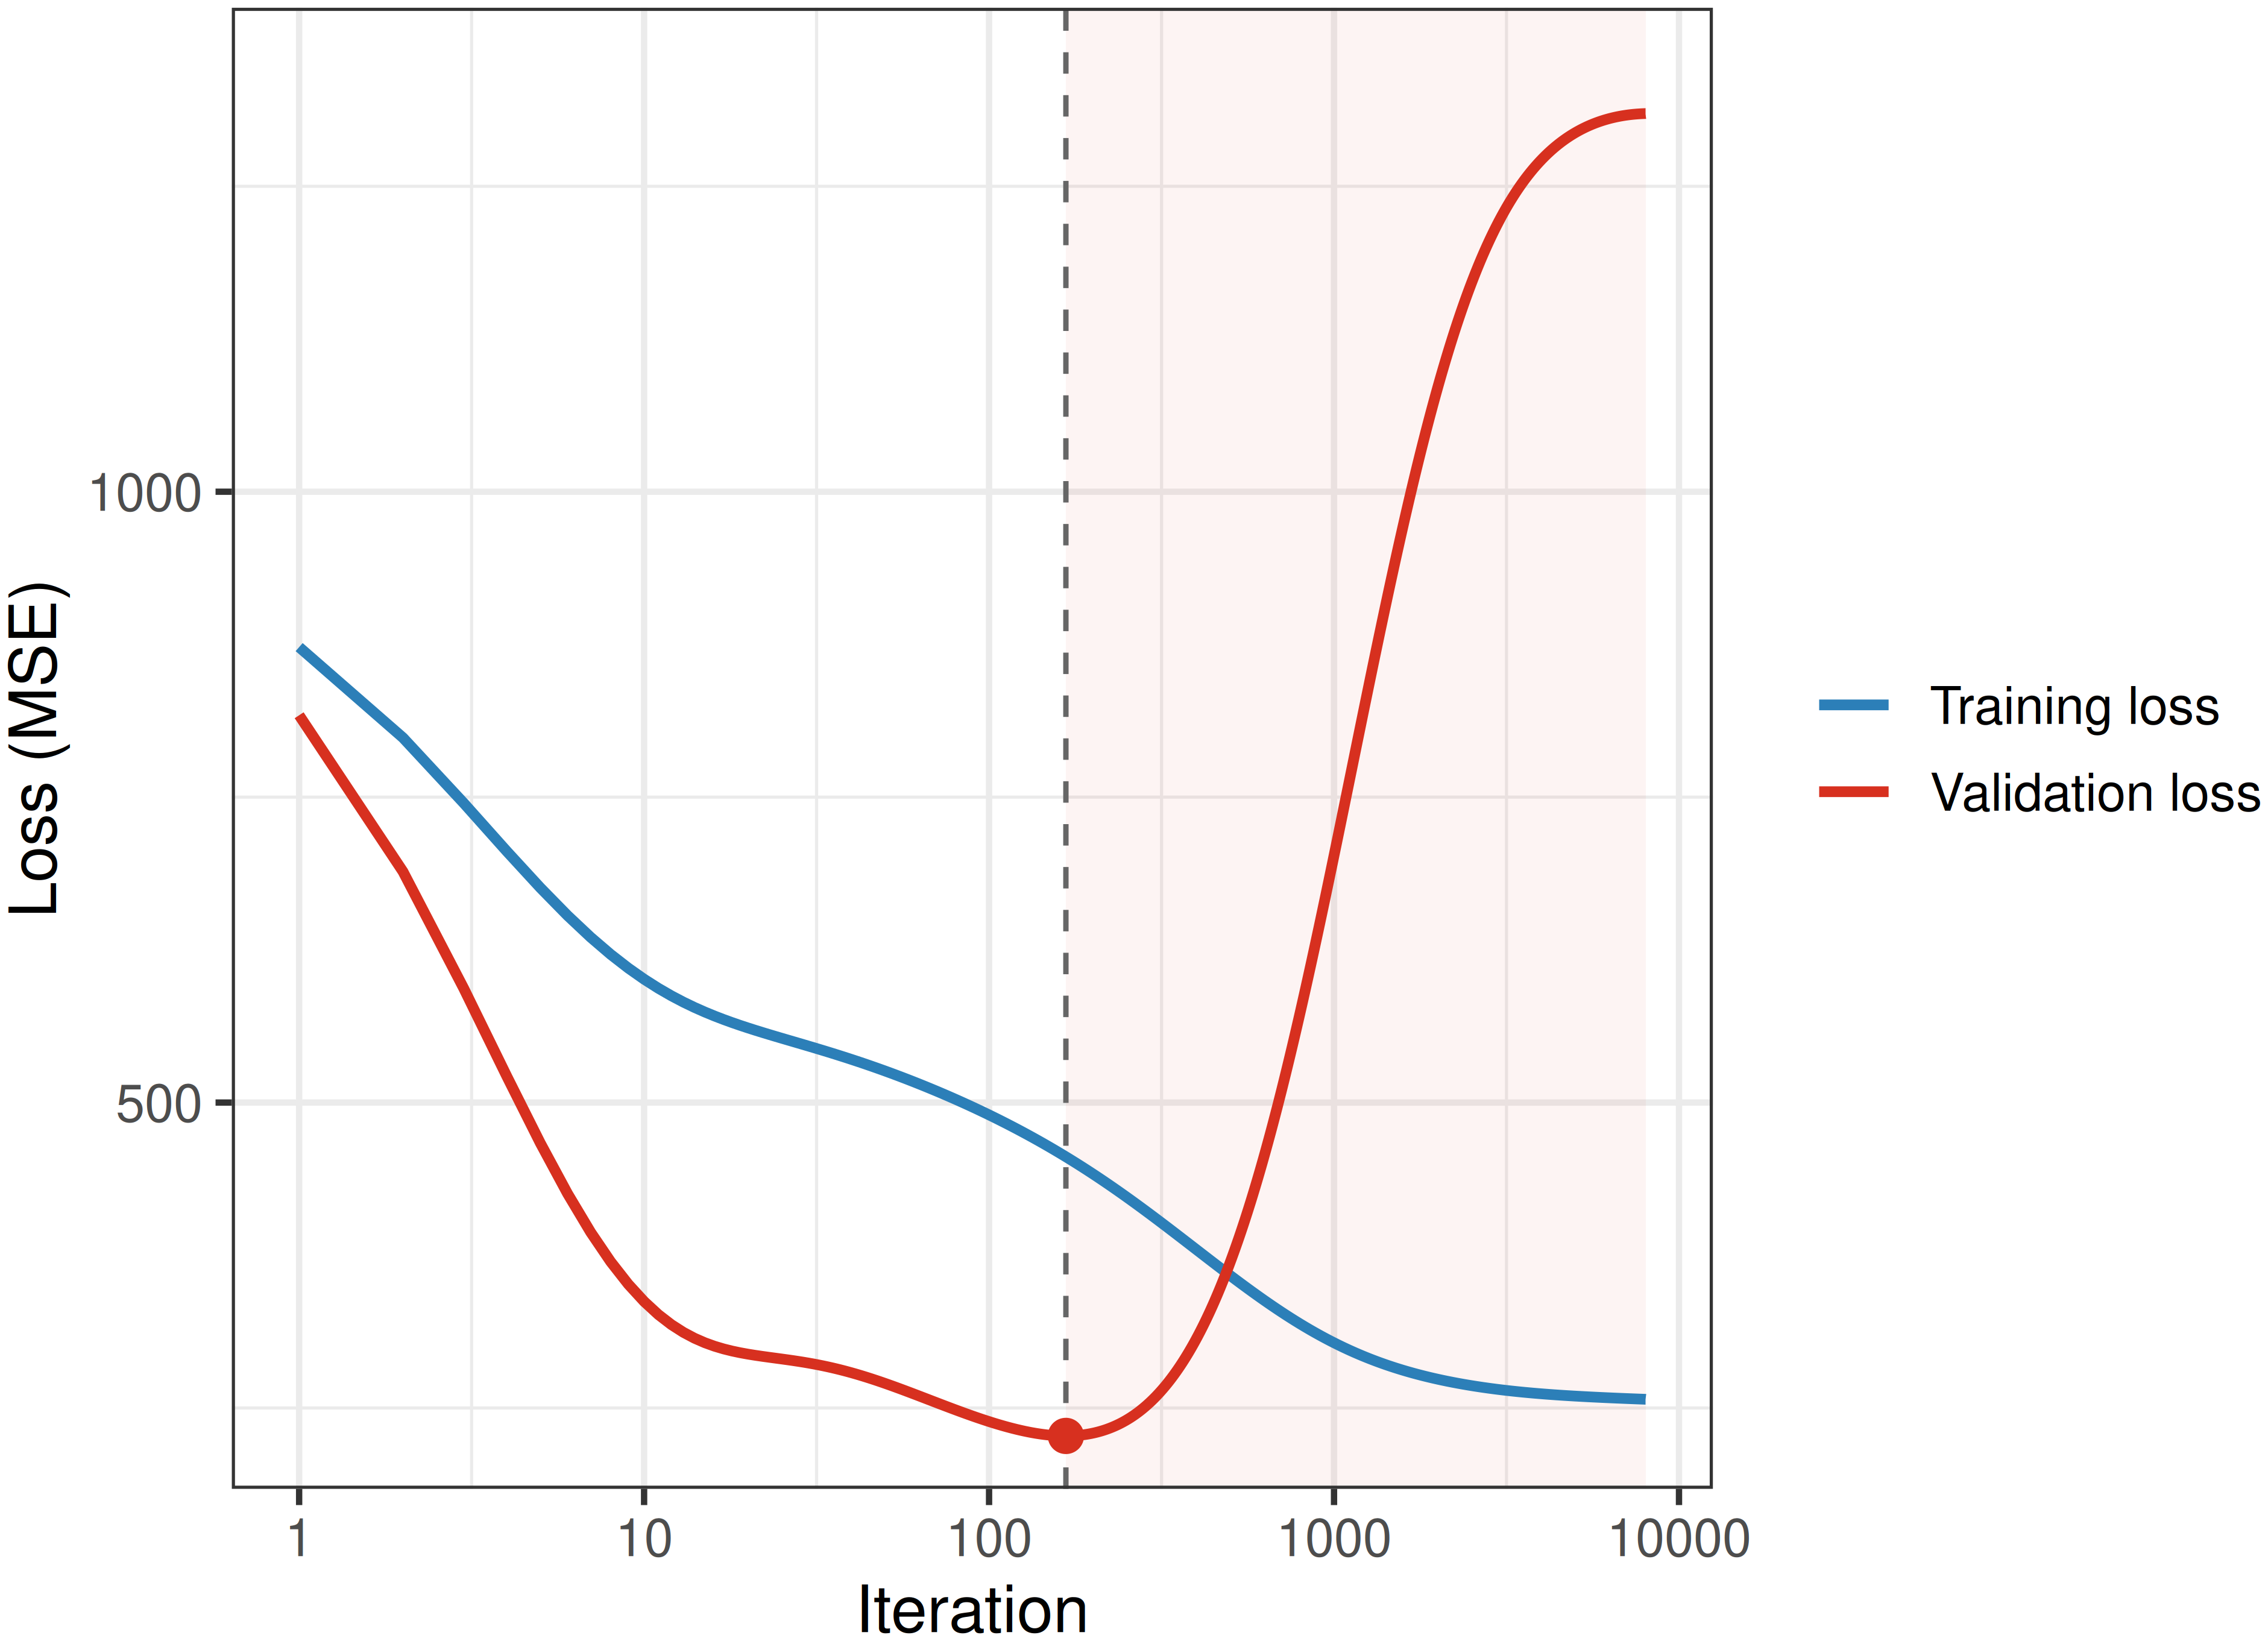
\includegraphics[width=0.7\linewidth,height=\textheight,keepaspectratio]{Figures/ml/fig-p1c3-early-stopping.png}

}

\caption{\label{fig-p1c3-early-stopping}Early stopping on the
gradient-descent example (Section~\ref{sec-ml-gradient-descent}), with
part of the data used for training and the rest for validation. As
gradient descent proceeds, the training loss decreases steadily, whereas
the validation loss first decreases and then increases as the model
begins to overfit. Early stopping returns the model from the iteration
with the lowest validation loss (dashed line); the shaded region marks
the overfitting iterations that are avoided.}

\end{figure}%

Theoretically, training could be stopped as soon as the validation loss
starts to increase, visualized by the red point in
Figure~\ref{fig-p1c3-early-stopping}. However, the validation loss
rarely improves smoothly from one iteration to the next, so a
\emph{patience} hyperparameter is used, which is the number of
consecutive iterations in which the validation loss must fail to improve
before stopping the training algorithm.\index{early stopping!patience}
Early stopping is computationally cheaper than tuning the number of
iterations directly (Section~\ref{sec-ml-opt}), which would require
repeatedly fitting complete models. Early stopping can also be viewed as
a form of regularization\index{regularization}, as limiting the number
of iterations restricts how closely the model can fit the training data,
in a similar spirit to how shrinkage or penalty terms constrain model
complexity.

\section{Conclusion}\label{conclusion}

\begin{tcolorbox}[enhanced jigsaw, toprule=.15mm, bottomtitle=1mm, opacityback=0, breakable, leftrule=.75mm, title={Key takeaways}, toptitle=1mm, bottomrule=.15mm, colback=white, colframe=quarto-callout-warning-color-frame, titlerule=0mm, opacitybacktitle=0.6, coltitle=black, rightrule=.15mm, left=2mm, colbacktitle=quarto-callout-warning-color!10!white, arc=.35mm]

\begin{itemize}
\tightlist
\item
  Machine learning tasks define the predictive problem of interest.
  Regression tasks make predictions for continuous outcomes, such as the
  amount of rain tomorrow. Classification tasks make predictions for
  discrete outcomes, such as if it will rain tomorrow (yes/no).
\item
  Both regression and classification tasks may make deterministic
  predictions (a single value or category), or probabilistic predictions
  (a probability distribution over values or categories).
\item
  Models have parameters that are learned during training and
  hyperparameters that are set or tuned.
\item
  Models should be evaluated on resampled data to estimate the
  generalization error to understand performance on new, unseen data.
\end{itemize}

\end{tcolorbox}

\begin{tcolorbox}[enhanced jigsaw, toprule=.15mm, bottomtitle=1mm, opacityback=0, breakable, leftrule=.75mm, title={Further reading}, toptitle=1mm, bottomrule=.15mm, colback=white, colframe=quarto-callout-tip-color-frame, titlerule=0mm, opacitybacktitle=0.6, coltitle=black, rightrule=.15mm, left=2mm, colbacktitle=quarto-callout-tip-color!10!white, arc=.35mm]

\begin{itemize}
\tightlist
\item
  \emph{The Elements of Statistical Learning} (Hastie, Tibshirani, and
  Friedman 2001), \emph{An Introduction to Statistical Learning} (James
  et al. 2013), and \emph{Pattern Recognition and Machine Learning}
  (Bishop 2006) for comprehensive introductions and overviews to machine
  learning.
\item
  \emph{Applied Machine Learning Using mlr3 in R} (Bischl et al. 2024)
  and \emph{Tidy Modeling} (Kuhn and Silge 2023) for machine learning in
  \(\textsf{R}\).
\item
  \emph{Hands-on Machine Learning with Scikit-Learn, Keras, and
  TensorFlow} (Géron 2019) for machine learning in Python.
\item
  Bischl et al. (2012) for discussions about more resampling strategies
  including bootstrapping and subsampling.
\end{itemize}

\end{tcolorbox}

\chapter{Survival Analysis}\label{sec-surv}

\emph{Survival analysis}\index{survival analysis} is the study of data
where the outcome is the time until an event takes place (a
`time-to-event'). Because the collection of such data takes place in the
temporal domain (it takes time to observe a duration), the event of
interest is often unobservable, for example because it did not occur by
the end of the data collection period. In survival analysis terminology
this is referred to as \emph{right-censoring},\index{censoring!right}
one of several censoring\index{censoring} mechanisms introduced below.

This chapter defines basic terminology and mathematical definitions in
survival analysis, which are used throughout this book. Building upon
this chapter, Chapter~\ref{sec-eha} introduces event history
analysis\index{event history analysis}, which is a generalization to
settings with multiple, potentially competing or recurrent
events\index{competing risks}\index{recurrent events}, including
multi-state outcomes\index{multi-state models}. Concluding this part of
the book, Chapter~\ref{sec-survtsk} defines different prediction
tasks\index{machine learning task} in survival analysis.

These definitions and concepts are standard in survival analysis, but
are presented explicitly here as precise familiarity with them is
essential for building successful models. Evaluation
functions\index{model evaluation} (Part II) can identify if one model is
better suited than another to minimize a given objective function.
However, they cannot identify whether the objective function itself is
correctly specified as that specification depends on assumptions about
the data-generating process. For example, the type(s) of
censoring/truncation present\index{censoring}\index{truncation}, whether
the censoring time \(C\) is independent of the event time \(Y\)
(marginally or conditionally on covariates \(X\)), and whether competing
events are present. Misstating these assumptions yields a mismatched
estimand: evaluating under these assumptions produces meaningless (even
if plausible looking) results. It is therefore vital for practitioners
to be able to identify and specify the survival problem present in their
data to ensure models are correctly fit and evaluated.

\section{Quantifying the distribution of event
times}\label{sec-distributions}

This section introduces functions that can be used to fully characterize
a probability distribution, with particular focus on functions that are
important in survival analysis.

In the temporal domain, events can either be recorded in discrete or
continuous time. For example, the number of rounds of chemotherapy
before remission would be recorded as a discrete-time
value\index{discrete-time survival analysis}. The number of rounds,
while still measured over time, can only take values in the positive
naturals, \(\mathbb{N}_{> 0}\). In contrast, if a practitioner were
instead recording the time to remission from the first round of
chemotherapy, then this may be recorded as the elapsed time between the
first treatment and remission, which is a continuous-time measurement
over the non-negative reals, \(\mathbb{R}_{\geq 0}\).

In practice, the differences between continuous and discrete time
measurements are often blurred. Time measurements are naturally
discretized at some level and precision beyond some resolution is often
not of interest. For example, length of stay in hospital could be
interesting up to days or even hours, but not minutes and seconds.
Software implementations of survival analysis techniques usually rely on
continuous-time theory, and continuous-time methods are typically
applied even when the underlying data are technically discrete. It is
nevertheless important to make the distinction as it informs
mathematical treatment and definition of the different quantities
introduced below. Moreover, discrete-time methods can be applied to
continuous-time data (Chapter~\ref{sec-partition-based-reductions}) and
separate discussion is therefore important to understand those
techniques \index{reductions}.

\begin{tcolorbox}[enhanced jigsaw, toprule=.15mm, bottomtitle=1mm, opacityback=0, breakable, leftrule=.75mm, title={Handling events at \(\tau = 0\)}, toptitle=1mm, bottomrule=.15mm, colback=white, colframe=quarto-callout-note-color-frame, titlerule=0mm, opacitybacktitle=0.6, coltitle=black, rightrule=.15mm, left=2mm, colbacktitle=quarto-callout-note-color!10!white, arc=.35mm]

In the literature, continuous-time outcomes are usually defined on the
non-negative Reals, \(\tau \in \mathbb{R}_{\geq 0}\), which allows
events to occur at \(\tau = 0\). In practice, most model implementations
assume time lies on the positive Reals, \(\tau \in \mathbb{R}_{>0}\),
and therefore cannot accommodate events at \(\tau = 0\).

Although relatively uncommon, observations with \(\tau = 0\) do arise in
real data and must be addressed during data preprocessing before model
fitting. Some strategies include:

\begin{enumerate}
\def\labelenumi{\arabic{enumi}.}
\tightlist
\item
  Removing observations with \(t_i = 0\);
\item
  Replacing \(t_i = 0\) with a small positive constant \(\epsilon>0\);
\item
  Setting \(t_i\) to the smallest observed event time greater than zero.
\end{enumerate}

These choices are context-dependent and it is essential that any
decisions are clearly documented and justified.

\end{tcolorbox}

\subsection{Continuous time}\label{sec-distributions-continuous}

For this section, assume a continuous random variable \(Y\) taking
values in \(\mathbb{R}_{\geq 0}\). A standard representation of the
distribution of \(Y\) is given by the probability density
function\index{probability density function},
\(f_Y: \mathbb{R}_{\geq 0}\rightarrow \mathbb{R}_{\geq 0}\), and
cumulative distribution
function\index{cumulative distribution function},
\(F_Y: \mathbb{R}_{\geq 0}\rightarrow [0,1]; F_Y(\tau) = \Pr(Y \leq \tau)\).

In survival analysis, it is more common to describe the distribution of
event times \(Y\) via the \emph{survival
function}\index{survival function} and \emph{hazard function} (or
\emph{hazard rate})\index{hazard function} rather than the probability
density function or cumulative distribution function. The survival
function is defined as:

\begin{equation}\phantomsection\label{eq-surv-prob}{
S_Y(\tau) = \Pr(Y > \tau) = \int^\infty_\tau f_Y(u) \ \,\mathrm{d}u,
}\end{equation}

which is the probability that an event has not occurred by
\(\tau \geq 0\) and thus the complement of the cumulative distribution
function: \(S_Y(\tau) = 1-F_Y(\tau)\). By definition, \(S_Y(0)=1\) and
\(S(\tau)\rightarrow 0\) as \(\tau \rightarrow \infty\) for a
\emph{proper} event-time distribution; \emph{improper} distributions,
for which this limit is positive, are discussed at the end of this
section.\index{proper distribution}\index{improper distribution}

The hazard function is given by,
\begin{equation}\phantomsection\label{eq-continuous-hazard}{
\begin{aligned}
h_Y(\tau) &= \lim_{\,\mathrm{d}\tau\searrow 0}\frac{\Pr(\tau  \leq Y < \tau + \,\mathrm{d}\tau\mid Y \geq \tau)}{\,\mathrm{d}\tau} \\
          &= \lim_{\,\mathrm{d}\tau\searrow 0}\frac{\Pr(Y \in [\tau, \tau + \,\mathrm{d}\tau) \mid Y \geq \tau)}{\,\mathrm{d}\tau}\\
          & = \frac{f_Y(\tau)}{S_Y(\tau)},
\end{aligned}
}\end{equation}

where \(\,\mathrm{d}\tau\) denotes a time-interval. The hazard rate is
often interpreted as the instantaneous risk of observing an event at
\(\tau\), given that the event has not been observed before \(\tau\).
This is not a probability and \(h_Y\) can be greater than one.

It is worth noting two particular points about the hazard function.
First, the hazard is a rate per unit time, which means its numerical
value depends on the scale on which \(\tau\) is measured. A hazard of
\(0.01\) on a daily scale equals \(3.65\) on an annual scale for the
same underlying process. Second, hazards are the natural modeling target
in survival analysis because censoring affects them locally. At a given
\(\tau\), only the subjects still at risk contribute to the hazard rate,
so it can be estimated from the event and risk-set counts at that time
point alone. The full survival trajectory up to \(\tau\) is not
required, which would itself require uncensored follow-up over
\([0, \tau]\). For a book-length treatment of the hazard rate and its
uses, see Rinne (2014).

The cumulative hazard function\index{cumulative hazard function} can be
derived from the hazard function by,

\[
H_Y(\tau) = \int^\tau_0 h_Y(u) \ \,\mathrm{d}u,
\]

and relates to the survival function via,

\[
\begin{aligned}
H_Y(\tau) & = \int^\tau_0 h_Y(u) \ \,\mathrm{d}u= \int^\tau_0 \frac{f_Y(u)}{S_Y(u)} \ \,\mathrm{d}u\\
          & = \int^\tau_0 -\frac{S'_Y(u)}{S_Y(u)} \ \,\mathrm{d}u= -\log(S_Y(\tau)).
\end{aligned}
\]

These last relationships are particularly important, as many methods
estimate the hazard function, which is then used to calculate the
cumulative hazard and survival probability,

\begin{equation}\phantomsection\label{eq-surv-haz}{
S_Y(\tau) = \exp(-H_Y(\tau)) = \exp\left(-\int_0^\tau h_Y(u)\ \,\mathrm{d}u\right).
}\end{equation}

Unless necessary to avoid confusion, subscripts are dropped from
\(S_Y, h_Y\), and other distribution-defining functions going forward.
Table~\ref{tbl-dist-transformations} summarizes the transformations
between the distribution-defining functions. As discussed in
Chapter~\ref{sec-intro}, the survival and hazard functions are the
natural target for predicted survival models. In practice, if the
survival function is targeted by a model then the density function is
estimated through linear interpolation and the remaining functions
follow through (\ref{eq-surv-prob})-(\ref{eq-surv-haz}). Otherwise, if
the hazard function is the target then the cumulative hazard can be
estimated through numerical integration, and again the other functions
follow through (\ref{eq-surv-prob})-(\ref{eq-surv-haz}).

\begin{longtable}[]{@{}
  >{\raggedright\arraybackslash}p{(\linewidth - 8\tabcolsep) * \real{0.2000}}
  >{\raggedright\arraybackslash}p{(\linewidth - 8\tabcolsep) * \real{0.2000}}
  >{\raggedright\arraybackslash}p{(\linewidth - 8\tabcolsep) * \real{0.2000}}
  >{\raggedright\arraybackslash}p{(\linewidth - 8\tabcolsep) * \real{0.2000}}
  >{\raggedright\arraybackslash}p{(\linewidth - 8\tabcolsep) * \real{0.2000}}@{}}
\caption{Transformations from one distribution-defining function (rows)
to another (columns).}\label{tbl-dist-transformations}\tabularnewline
\toprule\noalign{}
\begin{minipage}[b]{\linewidth}\raggedright
\end{minipage} & \begin{minipage}[b]{\linewidth}\raggedright
\(f(\tau)\)
\end{minipage} & \begin{minipage}[b]{\linewidth}\raggedright
\(h(\tau)\)
\end{minipage} & \begin{minipage}[b]{\linewidth}\raggedright
\(H(\tau)\)
\end{minipage} & \begin{minipage}[b]{\linewidth}\raggedright
\(S(\tau)\)
\end{minipage} \\
\midrule\noalign{}
\endfirsthead
\toprule\noalign{}
\begin{minipage}[b]{\linewidth}\raggedright
\end{minipage} & \begin{minipage}[b]{\linewidth}\raggedright
\(f(\tau)\)
\end{minipage} & \begin{minipage}[b]{\linewidth}\raggedright
\(h(\tau)\)
\end{minipage} & \begin{minipage}[b]{\linewidth}\raggedright
\(H(\tau)\)
\end{minipage} & \begin{minipage}[b]{\linewidth}\raggedright
\(S(\tau)\)
\end{minipage} \\
\midrule\noalign{}
\endhead
\bottomrule\noalign{}
\endlastfoot
\(f(\tau)\) & --- &
\(\frac{f(\tau)}{\int^\infty_\tau f(u)\ \,\mathrm{d}u}\) &
\(-\log\left(\int^\infty_\tau f(u)\ \,\mathrm{d}u\right)\) &
\(\int^\infty_\tau f(u)\ \,\mathrm{d}u\) \\
\(h(\tau)\) &
\(h(\tau)\exp\left(-\int_0^\tau h(u)\ \,\mathrm{d}u\right)\) & --- &
\(\int_0^\tau h(u)\ \,\mathrm{d}u\) &
\(\exp\left(-\int_0^\tau h(u)\ \,\mathrm{d}u\right)\) \\
\(H(\tau)\) & \(H'(\tau)\exp(-H(\tau))\) & \(H'(\tau)\) & --- &
\(\exp(-H(\tau))\) \\
\(S(\tau)\) & \(-S'(\tau)\) & \(-\frac{S'(\tau)}{S(\tau)}\) &
\(-\log(S(\tau))\) & --- \\
\end{longtable}

\subsubsection*{Proper and improper event
times}\label{proper-and-improper-event-times}

The formal definitions above take \(Y\) to be a \emph{proper} random
variable\index{proper distribution}, which means \(S_Y(\tau) \to 0\) as
\(\tau \to \infty\). However, many real-world events are \emph{improper}
at the population level\index{improper distribution},
\(S_Y(\infty) = \pi_0 > 0\), which practically means the event is not
guaranteed to occur. To continue an example from the introduction, when
modeling the time between relapses from multiple sclerosis, not every
patient will experience a relapse. The value \(\pi_0\) is known as the
\emph{cure fraction}, for a full treatment of \emph{cure models} see
(Lambert 2007; Maller and Zhou 1996)\index{cure models}.

In practice, for the predictive targets in this book, improper
distributions are rarely an obstacle as predictions live on a finite
horizon \([0, \tau^*]\) on which \(S(\tau)\) and \(h(\tau)\) are
well-defined regardless of properness of \(Y\) when
\(\tau \in [0, \tau^*]\). A quantity that is particularly sensitive to
properness is the \emph{mean} survival time
\(\mathbb{E}[Y] = \int_0^\infty S_Y(u)\,\,\mathrm{d}u\), which diverges
for improper \(Y\). The \emph{restricted mean survival time}
(RMST)\index{restricted mean survival time}
\(\int_0^{\tau^*} S_Y(u)\,\,\mathrm{d}u\) is often used as a
finite-horizon replacement (Section~\ref{sec-survtsk-time}). Informal
phrasings later in the chapter such as ``the event may occur later in
life'' should be read as ``later than the observation window'', not as
an assertion that \(Y\) is proper.

\subsection{Discrete time}\label{sec-distributions-discrete}

Now let \(\tilde{Y}\) be a random variable that represents discrete or
discretized time, taking values in
\(\mathbb{N}_{> 0}\)\index{discrete-time survival analysis}.

The discrete-time hazard function is defined as,

\begin{equation}\phantomsection\label{eq-discrete-hazard}{
h_{\tilde{Y}}(\tau) = \Pr(\tilde{Y}=\tau \mid \tilde{Y} \geq \tau).
}\end{equation}

Thus, in contrast to the continuous-time hazard
(\ref{eq-continuous-hazard}), the discrete-time hazard is an actual
(conditional) probability, rather than a rate and can therefore be
easier to interpret.

The cumulative discrete-time hazard is given by,

\begin{equation}\phantomsection\label{eq-discrete-cumu-hazard}{
H_{\tilde{Y}}(\tau) = \sum_{k=1}^{\tau}h_{\tilde{Y}}(k).
}\end{equation}

The probability of surviving beyond \(\tau\) given survival until
\(\tau\), is given by,

\begin{equation}\phantomsection\label{eq-discrete-surviving}{
s_{\tilde{Y}}(\tau) = \Pr(\tilde{Y}> \tau \mid \tilde{Y} \geq \tau).
}\end{equation}

Conditional on survival to \(\tau\), the event either occurs at or after
\(\tau\), and hence (\ref{eq-discrete-surviving}) is the complement of
(\ref{eq-discrete-hazard}):

\[
s_{\tilde{Y}}(\tau) = 1 - h_{\tilde{Y}}(\tau).
\]

It follows that the unconditional probability to survive beyond time
point \(\tau\) is given by,

\begin{equation}\phantomsection\label{eq-discrete-surv-prob}{
S_{\tilde{Y}}(\tau) = \Pr(\tilde{Y} > \tau) = \prod_{k\leq\tau} s_{\tilde{Y}}(k) = \prod_{k\leq\tau}(1-h_{\tilde{Y}}(k)),
}\end{equation} and the unconditional probability for an event at time
\(\tau\) is \[
\Pr(\tilde{Y}=\tau) = S_{\tilde{Y}}(\tau-1) h_{\tilde{Y}}(\tau).
\] When applied to continuous time \(Y\), the follow-up is divided in
\(J\) disjoint intervals
\([a_0,a_{1}), \ldots, [a_{j-1},a_j), \ldots, [a_{J-1},a_{J}]\), such
that \[
Y \in [a_{j-1}, a_j) \Leftrightarrow \tilde{Y} = j
\]

Thus,

\[
h_{\tilde{Y}}(j) = \Pr(Y \in [a_{j-1},a_j) \mid Y \geq a_{j-1})
\]

and

\[
S_{\tilde{Y}}(j) = \Pr(Y > a_{j}) = S_Y(a_{j})
\]

Before moving on, note that the discrete-time cumulative hazard
\(H_{\tilde{Y}}(\tau)\) may be defined in one of two ways in the
literature. The additive form (\ref{eq-discrete-cumu-hazard}) is the
conventional choice, and the one used in this book. Under this
definition, the continuous-time identity \(S(\tau) = \exp(-H(\tau))\) no
longer holds, and survival is recovered through the product
(\ref{eq-discrete-surv-prob}) instead. An alternative convention defines

\[
H_{\tilde{Y}}(\tau) := -\log S_{\tilde{Y}}(\tau) = -\sum_{k=1}^{\tau}\log\bigl(1 - h_{\tilde{Y}}(k)\bigr),
\]

which preserves \(S = \exp(-H)\) exactly.

The two coincide in the small-hazard limit, where
\(-\log(1 - h_{\tilde{Y}}(k)) \approx h_{\tilde{Y}}(k)\), and both
converge to the continuous-time integral
\(H(\tau) = \int_0^\tau h(u)\,\,\mathrm{d}u\) as the discretization is
refined; for a unified product-integral treatment, see Aalen, Borgan,
and Gjessing (2008, sec. 3.2.4).

\section{Single-event, right-censored data}\label{sec-data-rc}

The complexity of survival analysis compared to other fields arises from
the fact that the outcome of interest is often only partially observed.
Formally, let

\begin{itemize}
\tightlist
\item
  \(X\) taking values in \(\mathbb{R}^p\) be the generative random
  variable representing the data \emph{features} (also known as
  \emph{covariates} or \emph{independent variables});
\item
  \(Y\) taking values in \(\mathbb{R}_{\geq 0}\) be the (partially
  unobservable) \emph{true survival time}; and
\item
  \(C\) taking values in \(\mathbb{R}_{\geq 0}\) be the (partially
  unobservable) \emph{true censoring time}.
\end{itemize}

In the presence of censoring,\index{censoring} \(C\), it is impossible
to fully observe the true outcome of interest, \(Y\). Instead, the
observable variables are defined by the random variables,

\begin{itemize}
\tightlist
\item
  \(T := \min\{Y,C\}\), the \emph{outcome time} (realizations are
  referred to as the \emph{observed outcome time}); and
\item
  \(\Delta := \mathbb{I}(Y = T) = \mathbb{I}(Y \leq C)\), the
  \emph{event indicator}\index{event indicator} (also known as the
  \emph{censoring} or \emph{status} indicator).
\end{itemize}

Together \((T,\Delta)\) is referred to as the \emph{survival outcome} or
\emph{survival tuple}\index{survival outcome} and they form the
dependent variables. The survival outcome provides a concise mechanism
for representing the outcome time and indicating which outcome (event or
censoring) took place.

A single-event right-censored \emph{survival
dataset}\index{survival dataset} is defined by
\(\mathcal{D}= \{(\mathbf{x}_i, t_i, \delta_i)\}_{i=1}^n\), where
\((t_i,\delta_i)\) are realizations of \((T_i, \Delta_i)\) and
\(\boldsymbol{\mathbf{x_i}} = ({x_i}_1 \ {x_i}_2 \cdots {x_i}_{p})^\top\)
is a vector of features.

A useful quantity to define is the set of unique, ordered event
times\index{unique event times}. For example, given survival data,
\(\{(t_1=6, \delta_1=0)\), \((t_2=1, \delta_2=1)\),
\((t_3=10,\delta_3=1)\), \((t_4=5,\delta_4=0)\),
\((t_5 =10,\delta_5=1)\}\) the unique ordered event times are
\(\{t_{(1)},  t_{(2)}\} = \{1,10\}\) as the censored observations and
duplicated times are all removed. Formally, let \(m\leq n\) be the
number of unique, observed event times. Then the \emph{unique, ordered
event times} are,

\begin{equation}\phantomsection\label{eq-unique-ordered-event-times}{
t_{(1)}<\cdots<t_{(m)}, \quad m\le n.
}\end{equation}

A common short-hand is to use the subscript `\((k)\)' as an index
referring to the observation that experienced the event at time
\(t_{(k)}\). For example, \((\mathbf{x}_{(k)}, t_{(k)}, \delta_{(k)})\)
would be the features and outcome for the observation that experienced
the event at \(t_{(k)}\), the \(k\)th ordered event time.

Finally, the following quantities are used frequently throughout this
book and survival analysis literature more generally. Let
\(\{(t_i, \delta_i)\}^n_{i=1}\) be observed survival outcomes.

The \emph{risk set at \(\tau\)}\index{risk set}, is the index-set of
observation units at risk for the event just before \(\tau\)

\begin{equation}\phantomsection\label{eq-risk-set}{
\mathcal{R}_\tau := \{i: t_i \geq \tau\},
}\end{equation}

where \(i\) is the index of an observation in the data. In a continuous
setting, `just before' refers to an infinitesimally smaller time than
\(\tau\). This infinitesimal window is unobservable in reality and as
such the risk set at \(\tau\) includes observations that experience the
event (or are censored) at \(\tau\). For right-censored data, the risk
set contains all observations in the initial state,
\(\mathcal{R}_0 = \{1,\ldots,n\}\), and the risk set decreases over
time,
\(\mathcal{R}_{\tau} \subseteq \mathcal{R}_{\tau'}, \forall \tau > \tau'\).

The \emph{number of observations at risk at
\(\tau\)}\index{number at risk} is the cardinality of the risk set at
\(\tau\),

\begin{equation}\phantomsection\label{eq-risk-set-n}{
n_\tau := \sum_i \mathbb{I}(t_i \geq \tau) = \vert \mathcal{R}_\tau \vert.
}\end{equation}

Finally, the \emph{number of events at \(\tau\)}\index{number of events}
is defined by,

\begin{equation}\phantomsection\label{eq-risk-set-d}{
d_\tau := \sum_i \mathbb{I}(t_i = \tau, \delta_i = 1)
}\end{equation}

For truly continuous variables, one might expect only one event to occur
at each observed event time: \(d_{t_{(k)}} = 1,\forall k\). In practice,
ties\index{ties} are often observed due to finite measurement precision,
such that \(d_{\tau} > 1\) occurs frequently in real-world datasets.

The quantities \(\mathcal{R}_\tau\), \(n_\tau\), and \(d_\tau\) underlie
many models and measures in survival analysis. Several
non-parametric\index{non-parametric estimator} and
semi-parametric\index{semi-parametric models} methods
(Chapter~\ref{sec-classical}) like the
Kaplan-Meier\index{Kaplan-Meier estimator} estimator (see
Section~\ref{sec-surv-km}) are based on the ratio \(d_\tau / n_\tau\).

Applied to the \texttt{tumor} example in
Table~\ref{tbl-surv-data-tumor}, these quantities are:

\begin{itemize}
\tightlist
\item
  \(\mathcal{R}_{1217} = \{1, 3, 5\}\)
\item
  \(n_{1217} = \vert \mathcal{R}_{1217} \vert = 3\)
\item
  \(d_{1217} = 1\)
\end{itemize}

\begin{longtable}[]{@{}
  >{\raggedleft\arraybackslash}p{(\linewidth - 10\tabcolsep) * \real{0.0976}}
  >{\raggedleft\arraybackslash}p{(\linewidth - 10\tabcolsep) * \real{0.0976}}
  >{\raggedright\arraybackslash}p{(\linewidth - 10\tabcolsep) * \real{0.1707}}
  >{\raggedright\arraybackslash}p{(\linewidth - 10\tabcolsep) * \real{0.3415}}
  >{\raggedleft\arraybackslash}p{(\linewidth - 10\tabcolsep) * \real{0.1220}}
  >{\raggedleft\arraybackslash}p{(\linewidth - 10\tabcolsep) * \real{0.1707}}@{}}
\caption{Subset of the \texttt{tumor} (Bender and Scheipl 2018)
time-to-event dataset. Rows are individual observations (ID),
\(\mathbf{x}_{\cdot j}\) columns are features, \(t\) is observed
time-to-event, \(\delta\) is the event
indicator.}\label{tbl-surv-data-tumor}\tabularnewline
\toprule\noalign{}
\begin{minipage}[b]{\linewidth}\raggedleft
id (\(i\))
\end{minipage} & \begin{minipage}[b]{\linewidth}\raggedleft
age \((\mathbf{x}_{\cdot 1})\)
\end{minipage} & \begin{minipage}[b]{\linewidth}\raggedright
sex \((\mathbf{x}_{\cdot 2})\)
\end{minipage} & \begin{minipage}[b]{\linewidth}\raggedright
complications \((\mathbf{x}_{\cdot 3})\)
\end{minipage} & \begin{minipage}[b]{\linewidth}\raggedleft
days (\(\mathbf{t}\))
\end{minipage} & \begin{minipage}[b]{\linewidth}\raggedleft
status (\(\boldsymbol{\delta}\))
\end{minipage} \\
\midrule\noalign{}
\endfirsthead
\toprule\noalign{}
\begin{minipage}[b]{\linewidth}\raggedleft
id (\(i\))
\end{minipage} & \begin{minipage}[b]{\linewidth}\raggedleft
age \((\mathbf{x}_{\cdot 1})\)
\end{minipage} & \begin{minipage}[b]{\linewidth}\raggedright
sex \((\mathbf{x}_{\cdot 2})\)
\end{minipage} & \begin{minipage}[b]{\linewidth}\raggedright
complications \((\mathbf{x}_{\cdot 3})\)
\end{minipage} & \begin{minipage}[b]{\linewidth}\raggedleft
days (\(\mathbf{t}\))
\end{minipage} & \begin{minipage}[b]{\linewidth}\raggedleft
status (\(\boldsymbol{\delta}\))
\end{minipage} \\
\midrule\noalign{}
\endhead
\bottomrule\noalign{}
\endlastfoot
1 & 71 & female & no & 1217 & 1 \\
2 & 70 & male & no & 519 & 0 \\
3 & 67 & female & yes & 2414 & 0 \\
4 & 58 & male & no & 397 & 1 \\
5 & 39 & female & yes & 1217 & 0 \\
6 & 59 & female & no & 268 & 1 \\
\end{longtable}

\begin{tcolorbox}[enhanced jigsaw, toprule=.15mm, bottomtitle=1mm, opacityback=0, breakable, leftrule=.75mm, title={Time-varying covariates and immortal time bias}, toptitle=1mm, bottomrule=.15mm, colback=white, colframe=quarto-callout-note-color-frame, titlerule=0mm, opacitybacktitle=0.6, coltitle=black, rightrule=.15mm, left=2mm, colbacktitle=quarto-callout-note-color!10!white, arc=.35mm]

This book focuses on prediction using baseline covariates, where all
covariate values are assumed known at a fixed starting point.

In some applications, covariates may change during follow-up, for
example due to repeated measurements, treatment changes, or disease
progression. These are commonly referred to as
\emph{time-varying}\index{time-varying covariates} or
\emph{time-dependent covariates}.

Time-varying covariates require particular care as their misuse can
introduce biases, including \emph{immortal time
bias}\index{immortal time bias}. For example, suppose a treatment can
only be received after three years of survival. Knowing that a patient
received the treatment therefore guarantees that they survived long
enough to receive it. If patients are incorrectly assigned to the
treatment group at baseline (\(\tau=0\)) rather than when treatment
actually begins (\(\tau=3\)), the model learns an artificial survival
advantage for treated patients, as they must have survived the initial
untreated period.

More generally, the same bias arises whenever a baseline covariate is
defined using information from after baseline (a form of temporal
leakage), for example a retrospective dataset that records
\texttt{treatment\ =\ 1} for any patient who was ever treated. The
standard remedy is to model treatment as a time-varying covariate that
switches on only at the actual treatment time, so the immortal
pre-treatment period is correctly attributed to the untreated state
(Lévesque et al. 2010; Suissa 2008); a landmark analysis is an
alternative (Suissa 2008). Equivalently, the process can be represented
as a multi-state model with a transition into the treated state at time
of treatment, although this makes the estimation of the treatment effect
less direct.

Full discussion of time-varying covariates is outside the current scope
and requires extensions to the standard survival analysis framework,
often involving more complex data structures and modeling assumptions.
Although, the reductions introduced in Part IV, particularly
partition-based reductions
(Chapter~\ref{sec-partition-based-reductions}), lend themselves to
modeling time-varying covariates. For classic texts on time-dependent
covariates, see Therneau and Grambsch (2000) and John D. Kalbfleisch and
Prentice (1980); for a specific focus on predictive modeling, see
Houwelingen and Putter (2011).

\end{tcolorbox}

\section{Types of censoring}\label{sec-types-of-censoring}

Three types of censoring are commonly defined in survival analysis:
right-censoring\index{censoring!right},
left-censoring\index{censoring!left}, and
interval-censoring\index{censoring!interval}. The latter can be viewed
as the most general case. Multiple types of censoring and/or
truncation\index{truncation} (Section~\ref{sec-truncation}) can occur in
any given dataset and it is important to identify which types are
present to correctly select and specify models and measures for the
data.

\subsection{Right-censoring}\label{sec-types-of-censoring-right}

Right-censoring is the most common form of censoring in survival
data\index{censoring!right}. It occurs when the event of interest was
not experienced during the observation period, which may happen because
it was no longer observable (for example, due to withdrawal from the
study) or because the event did not happen until study end. The exact
event time is unknown but it is known that, if the event occurs, this
will be after the observed censoring time, hence \emph{right}-censoring
(imagine a timeline from left to right as in
Figure~\ref{fig-p1c4-censoring}).

\begin{figure}

\centering{

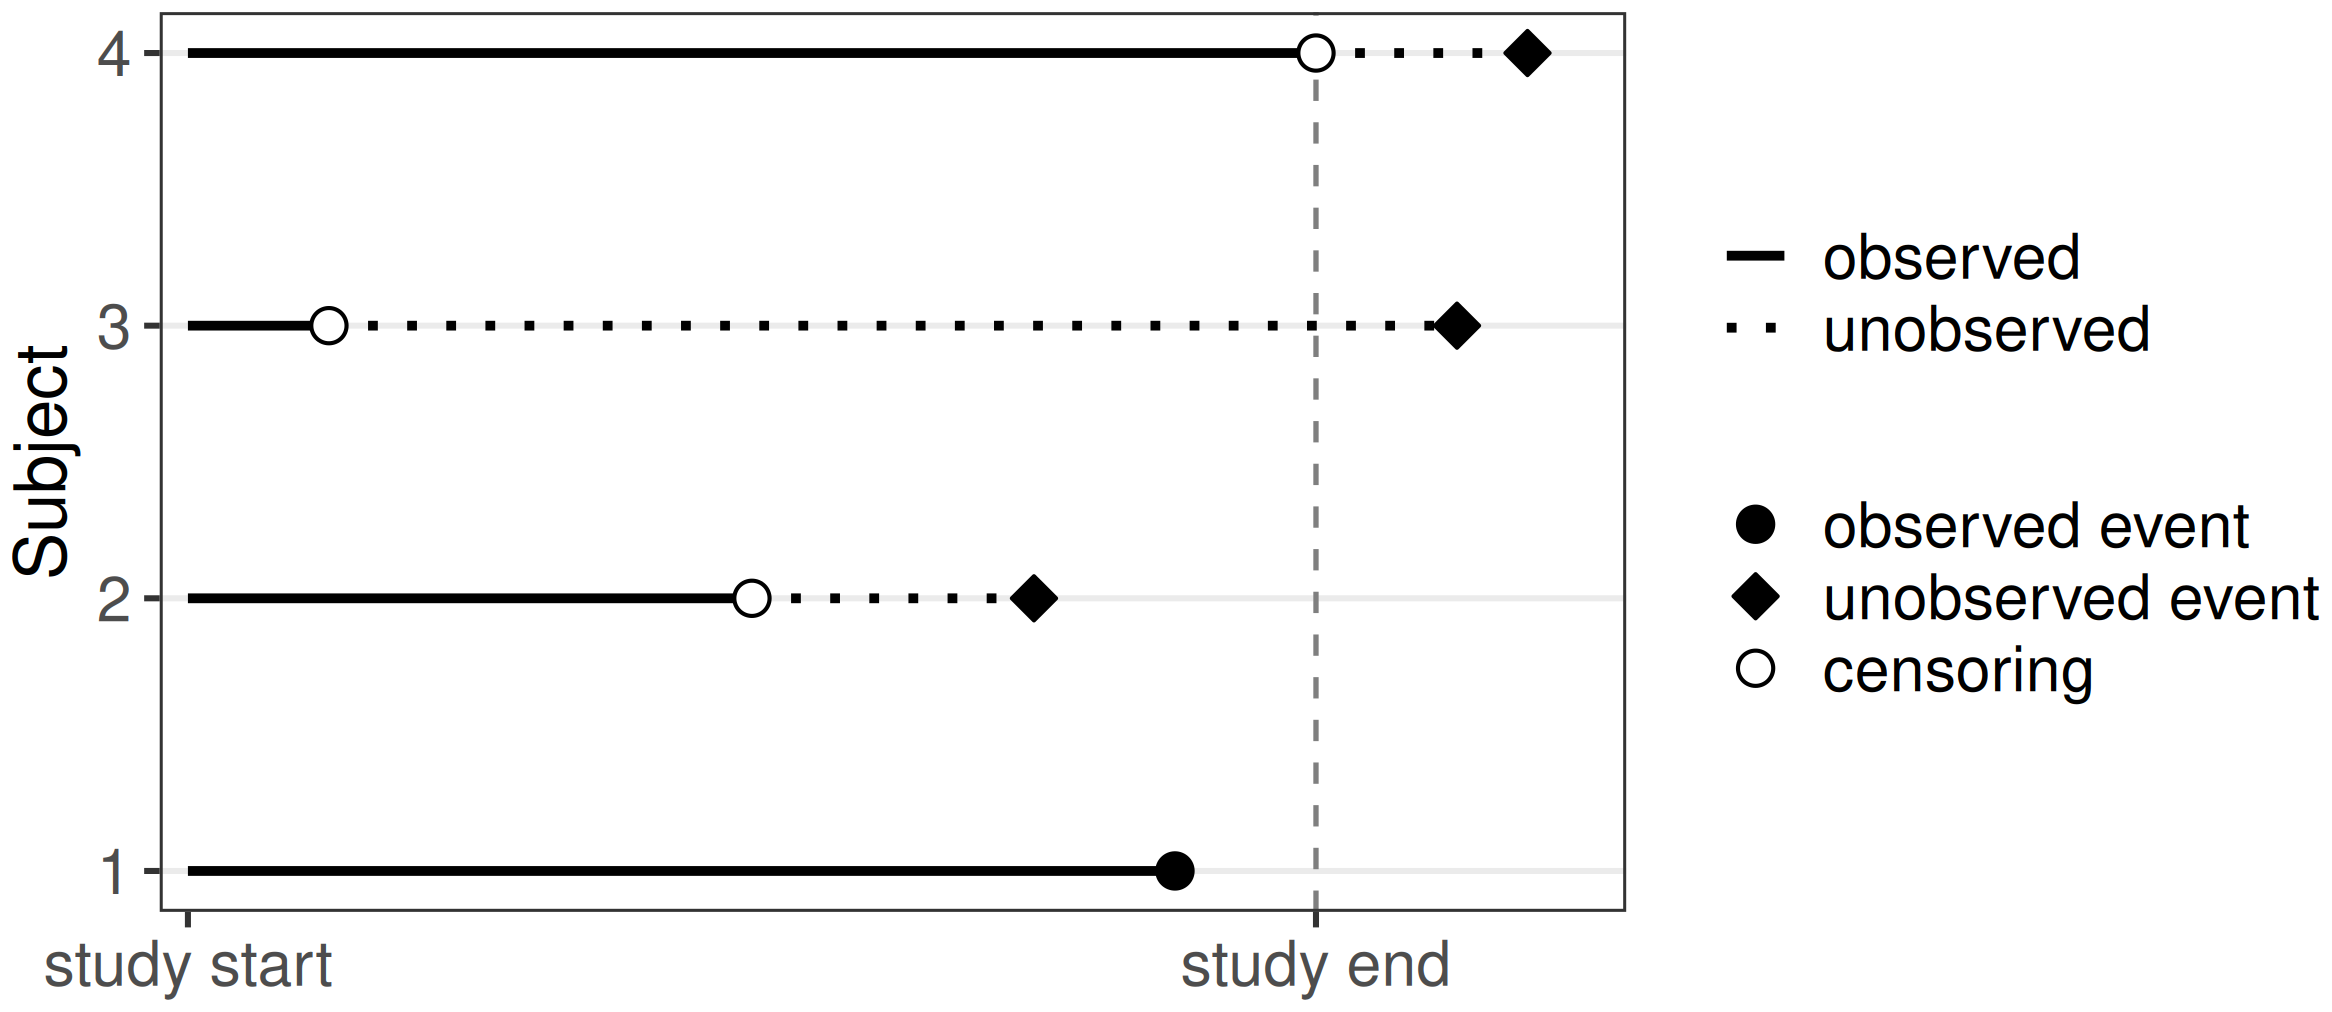
\includegraphics[width=1\linewidth,height=\textheight,keepaspectratio]{Figures/survival/fig-p1c4-censoring.png}

}

\caption{\label{fig-p1c4-censoring}Right-censoring for four subjects.
Solid lines mark observed periods, dotted lines mark hypothetical
(unknown in reality) post-censoring continuations. The vertical dashed
line marks the end of the study. Filled black circles mark observed
events, filled black diamonds mark true (unobserved) event times, and
open circles mark censoring. Subject 1's event is observed during the
study. Subject 2 is censored during the study and would have died during
the study (unobserved). Subject 3 is censored early in the study and
dies after study end (unobserved). Subject 4 is administratively
censored at study end and dies later (unobserved).}

\end{figure}%

Right-censoring can be further divided into type
I\index{censoring!type I}, type II\index{censoring!type II} and random
censoring\index{censoring!random}.

Random censoring occurs when censoring times \emph{randomly} follow an
unknown distribution and one observes
\((T_i=\min(Y_i,C_i), \Delta_i = \mathbb{I}(Y_i\leq C_i))\).

Type I, or \emph{administrative}, censoring occurs at the fixed,
pre-defined end of an observation period \(\tau_u\), in which case the
outcome is given by
\((T_i = \min(Y_i, \tau_u), \Delta_i = \mathbb{I}(Y_i \leq \tau_u))\).
The survival outcome of these observations is represented as
\((\tau_u, 0)\). In practice, \(\tau_u\) is often subject-dependent,
\(\tau_{u,i}\), due to \emph{staggered entry}\index{staggered entry},
meaning that subjects enter the study at different calendar times while
study end is defined by a fixed calendar end-date. Each subject's
administrative censoring time is then the difference between study
closure and individual entry.

Type II censoring also occurs when the observation period ends. However,
in this case the study concludes when a pre-defined number of subjects
experienced the event of interest.

Different types of right-censoring can, and do, co-occur in any given
dataset. In practice, these different types of right-censoring are
usually handled the same during modeling and evaluation and so this book
refers to `right-censoring' generally.

\subsection{Left- and
interval-censoring}\label{sec-types-of-censoring-left-interval}

Left-censoring\index{censoring!left} occurs when the event is known to
have happened at some unknown time before the observation time.
Interval-censoring\index{censoring!interval} occurs when the event is
known to have happened within some time range, but the exact time is
unknown.

Consider a survey in which participants are asked ``how old were you
when you used a smartphone for the first time?''. The possible answers
from a participant are:

\begin{itemize}
\tightlist
\item
  the exact age of first use; or
\item
  not applicable as they have never used a smartphone; or
\item
  they use, or previously have used, a smartphone but they do not
  remember their age the first time; or
\item
  they use, or previously have used, a smartphone but they only recall
  the age range of first use.
\end{itemize}

The first case represents an exactly observed event time. The second
case is right-censoring as the event may occur later in life but it is
unknown when. The third case is referred to as left-censoring, the event
occurred some time before the survey. The fourth case is an example of
interval-censoring, the event occurred within some age range but the
exact age is unknown.

Interval-censoring is pervasive in medicine whenever events are
detectable only at follow-up visits. For example, in HIV cohort studies
the exact time of seroconversion is unknown; it lies in the interval
between the last negative test and the first positive test (Z. Zhang and
Sun 2010). Handling of interval-censoring depends on the modeling time
scale. For example, consider a patient in the second year of the HIV
cohort study who receives a positive test in July. If a predictive model
is defined at the level of calendar years, the event can be assigned to
year \(2\) and treated as observed, ignoring the within-year timing
uncertainty that a finer time scale would have to handle as
interval-censoring. More generally, if the chosen resolution is coarser
than the typical interval width, interval-censored observations can be
treated as approximately observed events at that scale. In all other
cases, interval-censoring requires dedicated estimators (see
Section~\ref{sec-surv-estimation}).

\subsection{Censoring notation}\label{sec-types-of-censoring-notation}

In the presence of left- or interval-censoring the usual representation
of survival outcomes as \((t_i, \delta_i)\) is not sufficient to denote
the different types of observations in the dataset. Instead,
observations are represented as intervals in which the event occurs.
Formally, let \(Y_i\) be the random variable for time until the event of
interest and \(L_i, R_i\) be random variables that define an interval
\((L_i,R_i]\) with realizations \(l_i, r_i\). Further, let \(t_i\) be
the time of observation (for example age at interview in the phone use
example) or last follow-up time for subject \(i\). Then, the event time
of subject \(i\) is:

\begin{itemize}
\tightlist
\item
  left-censored if \(Y_i \in (L_i = 0, R_i = t_i]\); or
\item
  right-censored if \(Y_i \in (L_i = t_i, R_i = \infty)\); or
\item
  interval-censored if \(Y_i \in (L_i = l_i, R_i = r_i]\),
  \(l_i < r_i \leq t_i\); or
\item
  exactly observed if \(Y_i \in (L_i = t_i, R_i = t_i]\).
\end{itemize}

With this notation it is clear that right- and left-censoring are
special cases of interval-censoring with left-censoring corresponding to
\((0, t_i]\) and right-censoring corresponding to \((t_i, \infty)\).

In the HIV seroconversion example above, \(r_i\) is the time of the
first positive test and \(l_i\) the time of the last negative test
before \(r_i\). In the phone survey example, suppose all participants
are interviewed at age \(18\). A participant might then specify any age
range between \(0\) and \(18\). Some examples are given in
(Table~\ref{tbl-censoring-phones}).

\begin{longtable}[]{@{}
  >{\raggedright\arraybackslash}p{(\linewidth - 6\tabcolsep) * \real{0.0769}}
  >{\raggedright\arraybackslash}p{(\linewidth - 6\tabcolsep) * \real{0.0769}}
  >{\raggedright\arraybackslash}p{(\linewidth - 6\tabcolsep) * \real{0.0769}}
  >{\raggedright\arraybackslash}p{(\linewidth - 6\tabcolsep) * \real{0.7692}}@{}}
\caption{Examples of censoring notation using age at first smartphone
use.}\label{tbl-censoring-phones}\tabularnewline
\toprule\noalign{}
\begin{minipage}[b]{\linewidth}\raggedright
id
\end{minipage} & \begin{minipage}[b]{\linewidth}\raggedright
\(l_i\)
\end{minipage} & \begin{minipage}[b]{\linewidth}\raggedright
\(r_i\)
\end{minipage} & \begin{minipage}[b]{\linewidth}\raggedright
Description
\end{minipage} \\
\midrule\noalign{}
\endfirsthead
\toprule\noalign{}
\begin{minipage}[b]{\linewidth}\raggedright
id
\end{minipage} & \begin{minipage}[b]{\linewidth}\raggedright
\(l_i\)
\end{minipage} & \begin{minipage}[b]{\linewidth}\raggedright
\(r_i\)
\end{minipage} & \begin{minipage}[b]{\linewidth}\raggedright
Description
\end{minipage} \\
\midrule\noalign{}
\endhead
\bottomrule\noalign{}
\endlastfoot
1 & 18 & \(\infty\) & No use yet at \(18\) (right-censored) \\
2 & 15 & 15 & First use at \(15\) (event) \\
3 & 14 & 16 & First use sometime between \(14\) and \(16\)
(interval-censored) \\
4 & 0 & 18 & First use sometime before \(18\) (left-censored) \\
\end{longtable}

An interesting distinction to note is that in the case of left- and
interval-censoring, it is \emph{guaranteed} that the event occurred,
either before the left-censoring time or within the given interval. In
the case of right-censoring, it is usually \emph{assumed} the event will
occur in \((t_i, \infty)\) (Section~\ref{sec-distributions-continuous});
under this assumption, censoring encodes uncertainty about \emph{when}
the event occurs, not uncertainty about \emph{whether} the event occurs.

\subsection{Independent and dependent
censoring}\label{independent-and-dependent-censoring}

Censoring is sometimes described as
\emph{non-informative}\index{censoring!non-informative} if \(Y\) and
\(C\) are independent\index{censoring!independent},
\(Y \perp \!\!\! \perp C\), which means that knowing the value of one
gives no information about the value of the other. However, this
definition could be misleading as the term `non-informative' may imply
that \(C\) is independent of both \(X\) \emph{and} \(Y\), and not just
\(Y\). To avoid misinterpretation, the following definitions are used in
this book:

\begin{itemize}
\tightlist
\item
  If \(C \perp \!\!\! \perp X\), censoring is
  \emph{feature-independent}, otherwise censoring is
  \emph{feature-dependent}.\index{censoring!dependent}
\item
  If \(C \perp \!\!\! \perp Y\), censoring is \emph{event-independent},
  otherwise censoring is \emph{event-dependent}.
\item
  If \(C \perp \!\!\! \perp Y  \mid  X\), censoring is conditionally
  independent of the event given covariates, or \emph{conditionally
  event-independent}.\index{censoring!conditionally independent}
\item
  If \(C \perp \!\!\! \perp(X,Y)\), censoring is \emph{marginally
  independent}.
\end{itemize}

Marginally independent censoring is the strongest assumption and implies
that censoring does not depend on either covariates or the event time.
In this setting, standard survival estimators can recover the underlying
survival distribution without bias. However, censored observations still
contain partial information and should not be discarded as doing so
reduces efficiency and can introduce bias in finite samples.

The majority of models and measures assume conditionally
event-independent censoring, meaning that once conditioned on observed
features, the censoring time provides no additional information about
the event time. Type I and type
II\index{censoring!type I}\index{censoring!type II} censoring
(Section~\ref{sec-types-of-censoring-right}) are usually conditionally
event-independent, as the censoring mechanism is determined by study
design or stopping rules rather than the underlying event process.
Censoring can still depend on covariates while remaining conditionally
event-independent: for example, patients with a more favorable prognosis
at study entry are often more likely to remain under observation for
longer and therefore have a higher probability of being censored.

In reality, the mechanisms that prevent the event of interest from being
observed are rarely independent, as dropout, incomplete follow-up, and
intervening events tend to be related to the outcome under study. Two
cases are especially important to distinguish: dependent censoring and
competing risks. Under \emph{event-dependent}
censoring\index{censoring!dependent}, \(C \not\!\perp\!\!\!\perp Y\),
the censoring time carries information about the event time; treating
censoring as independent can lead to biased estimates and miscalibrated
predictions. When this dependence is fully captured by measured
covariates, that is, censoring is conditionally event-independent given
those covariates, this bias can be corrected by reweighting observations
(Robins and Finkelstein 2000) with inverse probability of censoring
weights (Section~\ref{sec-surv-ipcw}). A \emph{competing
risk}\index{competing risks}, by contrast, is an event whose occurrence
precludes the event of interest from ever occurring, rather than merely
preventing its observation. Which case applies depends on the precise
definition of the event of interest: discharge from hospital, for
example, is often treated as a competing event because the event of
interest, \emph{in-hospital death} during the current stay, can no
longer occur once a patient has been discharged. Competing risks are
discussed in more detail in Chapter~\ref{sec-eha}.

\section{Censoring and truncation}\label{sec-truncation}

Censoring and truncation\index{truncation} are related but distinct
concepts and require substantially different methods to handle them. As
discussed in Chapter~\ref{sec-intro}, truncation in survival analysis
refers to partially truncating a period of time and is quite common in
the more general event history setting (Chapter~\ref{sec-eha}). In
particular, left-truncation plays an important role when modeling
recurrent events\index{recurrent events} or multi-state
data\index{multi-state models} (Section~\ref{sec-multi-state}). While
censored observations have incomplete information about the
time-to-event, they are still part of the dataset, whereas truncation
leads to observations not entering the dataset at all. This usually
introduces bias that must be resolved appropriately.

\subsection{Left-truncation}\label{sec-left-truncation}

Left-truncation\index{truncation!left} often arises when inclusion into
a study is conditional on the occurrence of another event. This means
observations have a subject-specific entry time, \(t^\ell_i\), also
known as their left-truncation time. Left-truncation has two important
consequences for the observed data; let \(t_i\) be the outcome time,
then

\begin{enumerate}
\def\labelenumi{\arabic{enumi}.}
\tightlist
\item
  if the subject experiences the event \emph{before} their entry time,
  \(t_i < t^\ell_i\), they never enter the dataset and so the sample is
  systematically biased toward longer event times;
\item
  if the subject \emph{does} enter the study, \(t_i \ge t^\ell_i\), then
  they are only observed from \(t_i^\ell > 0\) (known as \emph{delayed
  entry})\index{delayed entry}\index{selection bias}.
\end{enumerate}

Methods to handle these cases are discussed in
Section~\ref{sec-surv-estimation-param} and
Section~\ref{sec-non-param-lt}. Failing to account for left-truncation
results in biased estimators.

For illustration, consider a study from the 18th century (Broström
1987), when childhood and maternal mortality were relatively high. The
goal of the study was to establish the effect of a mother's death on
infant survival. Infants entered the study if and when their mother
died. By design, infants who died before their mothers could never enter
the study. A mother's death is the left-truncation event that determines
the left-truncation time, which here is the infant's age at study entry.

This is illustrated in Figure~\ref{fig-p1c4-left-truncation} for three
infants. For each infant, the upper bar shows the left-truncation time
\(t_i^\ell\) (age at the mother's death) and the lower bar the
time-to-event \(t_i\) (age at the infant's own death or, for infant 3,
censoring at study end at 365 days). Infant 1's own death occurs before
the mother's, so \(t_1 < t_1^\ell\) and the infant never enters the
dataset; both bars are drawn dotted to indicate they are not observed.
Infants 2 and 3 enter the study at their respective \(t_i^\ell\) and are
then followed: infant 2 dies during the study at \(t_2\), while infant 3
is alive at study end and is right-censored. In this example,
left-truncation biases the sample toward healthier infants, as frail
infants die earlier and thus on average before their mothers.

\begin{figure}

\centering{

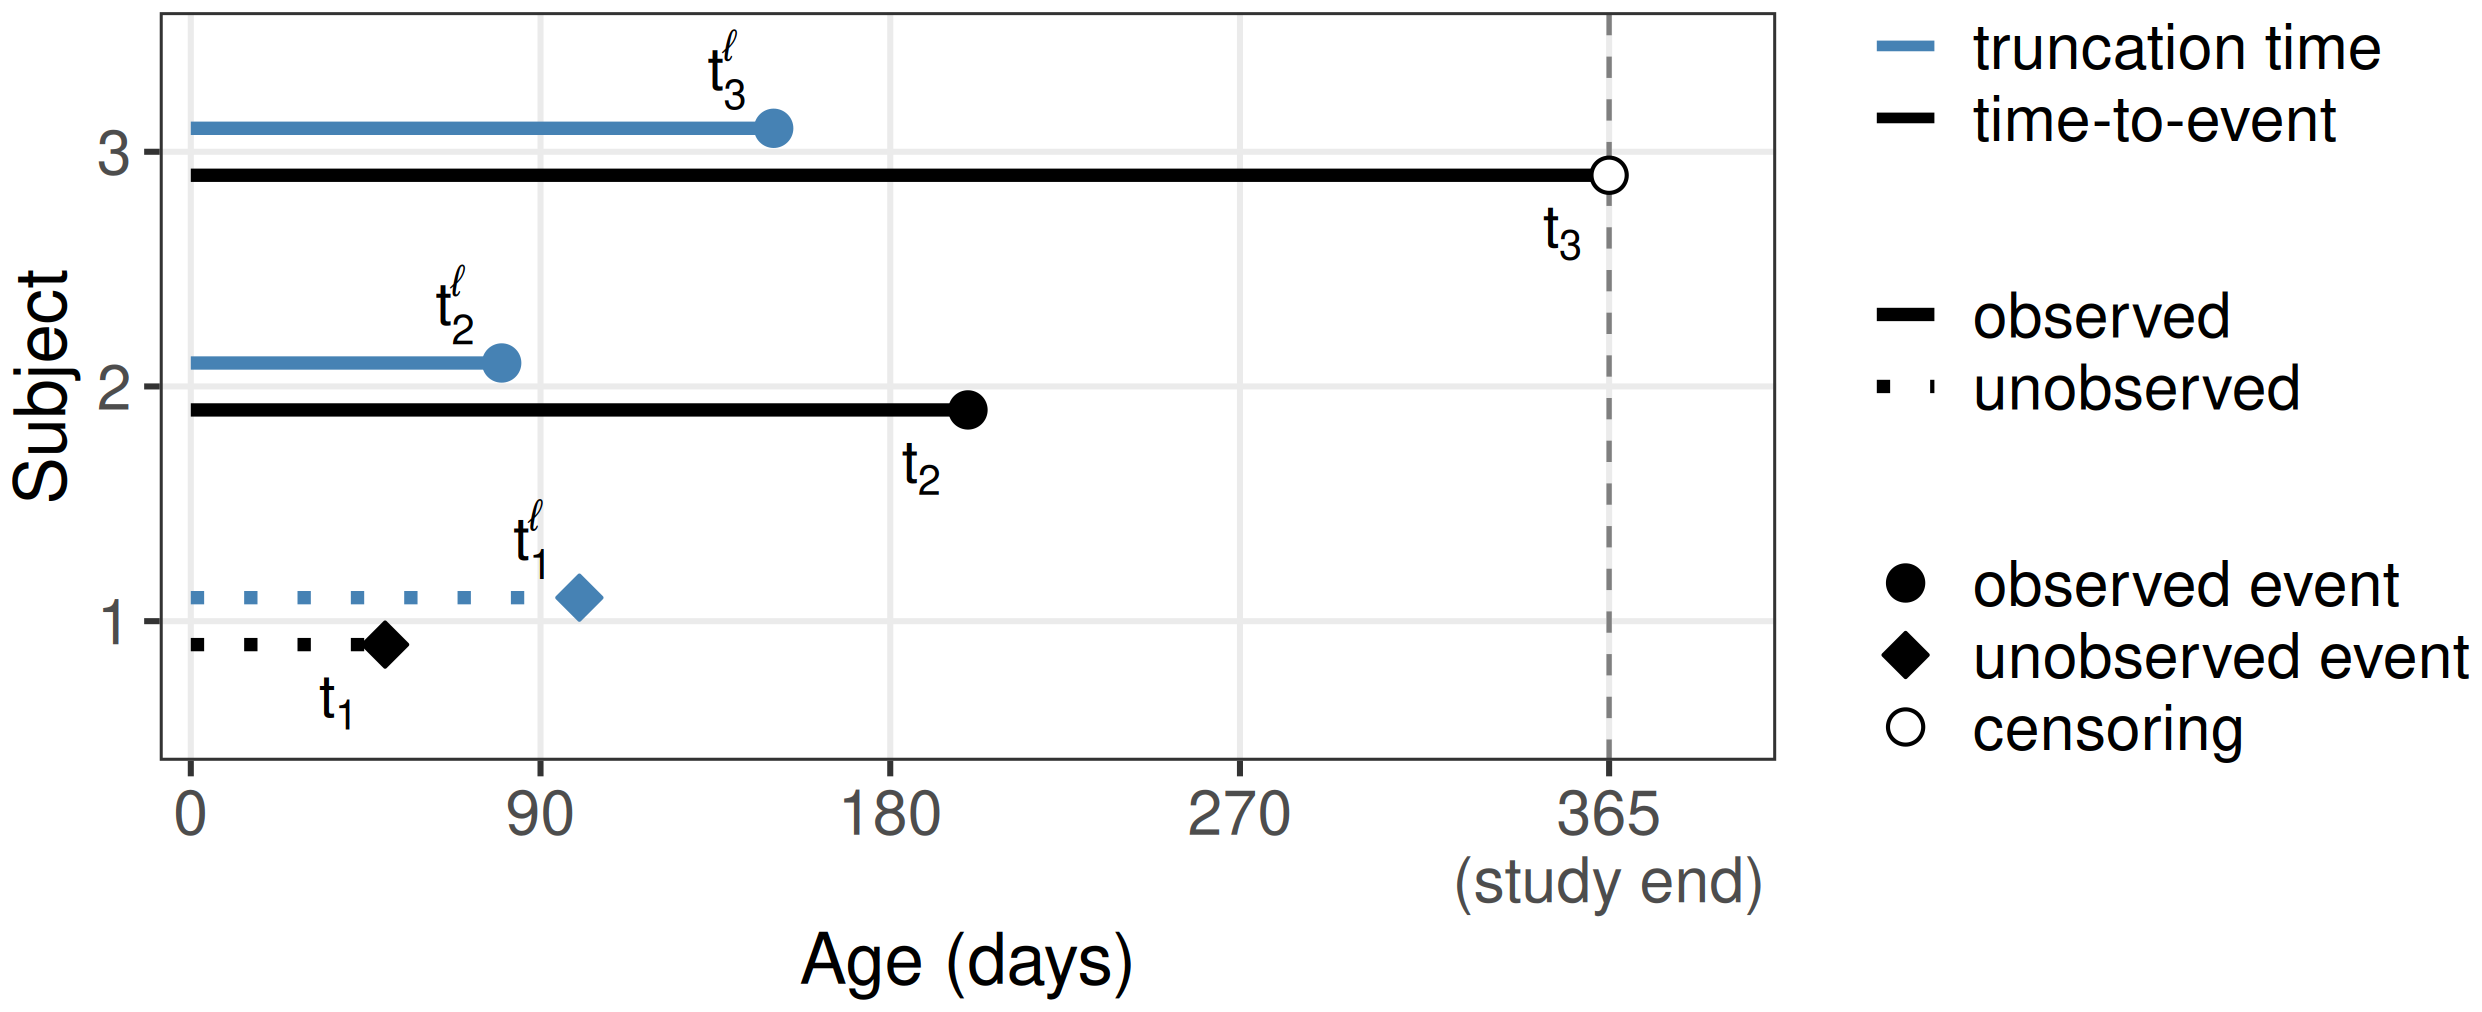
\includegraphics[width=1\linewidth,height=\textheight,keepaspectratio]{Figures/survival/fig-p1c4-left-truncation.png}

}

\caption{\label{fig-p1c4-left-truncation}Illustration of left-truncation
for three infants. For each subject, the upper steel blue bar shows the
truncation time \(t_i^\ell\) (age at mother's death) and the lower black
bar the time-to-event \(t_i\) (age at own death or censoring). Solid
lines mark in-sample subjects (\(t_i^\ell < t_i\)); dotted lines mark
the invisible subject 1 (\(t_1 < t_1^\ell\), infant dies before mother).
The truncation bar ends in a filled steel blue circle for in-sample
subjects and a filled steel blue diamond for the unobserved subject. The
vertical dashed line marks the study end at age 365 days. Filled black
circles, filled black diamonds, and open circles mark observed events,
unobserved events, and right-censoring respectively.}

\end{figure}%

\subsection{Right-truncation}\label{sec-right-truncation}

Right-truncation\index{truncation!right} often occurs in retrospective
sampling based on registry data, when data is queried for cases reported
by a certain cutoff time (see for example Vakulenko-Lagun, Mandel, and
Betensky (2020)). A common example is the estimation of the incubation
period of an infectious disease, which is the time from infection to the
disease onset. Only known, symptomatic (and/or tested) cases are entered
into the database. At a time \(\tau\), one can only observe the subset
of the infected population that has already experienced the disease, and
not the population that is still incubating the disease, hence biasing
the data to shorter incubation periods.

Formally, let \(t_i^r\) be the right-truncation time (here time from
infection until the time at which the database is queried), then
subjects only enter the dataset when \(t_i < t_i^r\). This is
illustrated in Figure~\ref{fig-p1c4-right-truncation} using three
subjects. All three subjects were infected during the observation
period, however, the right-truncation time of subject 2, \(t_2^r\), is
shorter than the incubation period for this subject, \(t_2\). Thus, at
the time of querying the database, this subject will not be included in
the sample, as \(t_2 > t_2^r\).

Note the difference to right-censoring\index{censoring!right}. If
subject 2 was right-censored, the subject would be in the sample with a
known time of infection and the time of disease onset would be censored.
In case of right-truncation on the other hand, the subject is not
included in the sample at time of data extraction, as subjects are only
included in the registry after disease onset. Overall this leads to a
bias toward shorter incubation times and potentially feature values that
lead to shorter incubation times.

\begin{figure}

\centering{

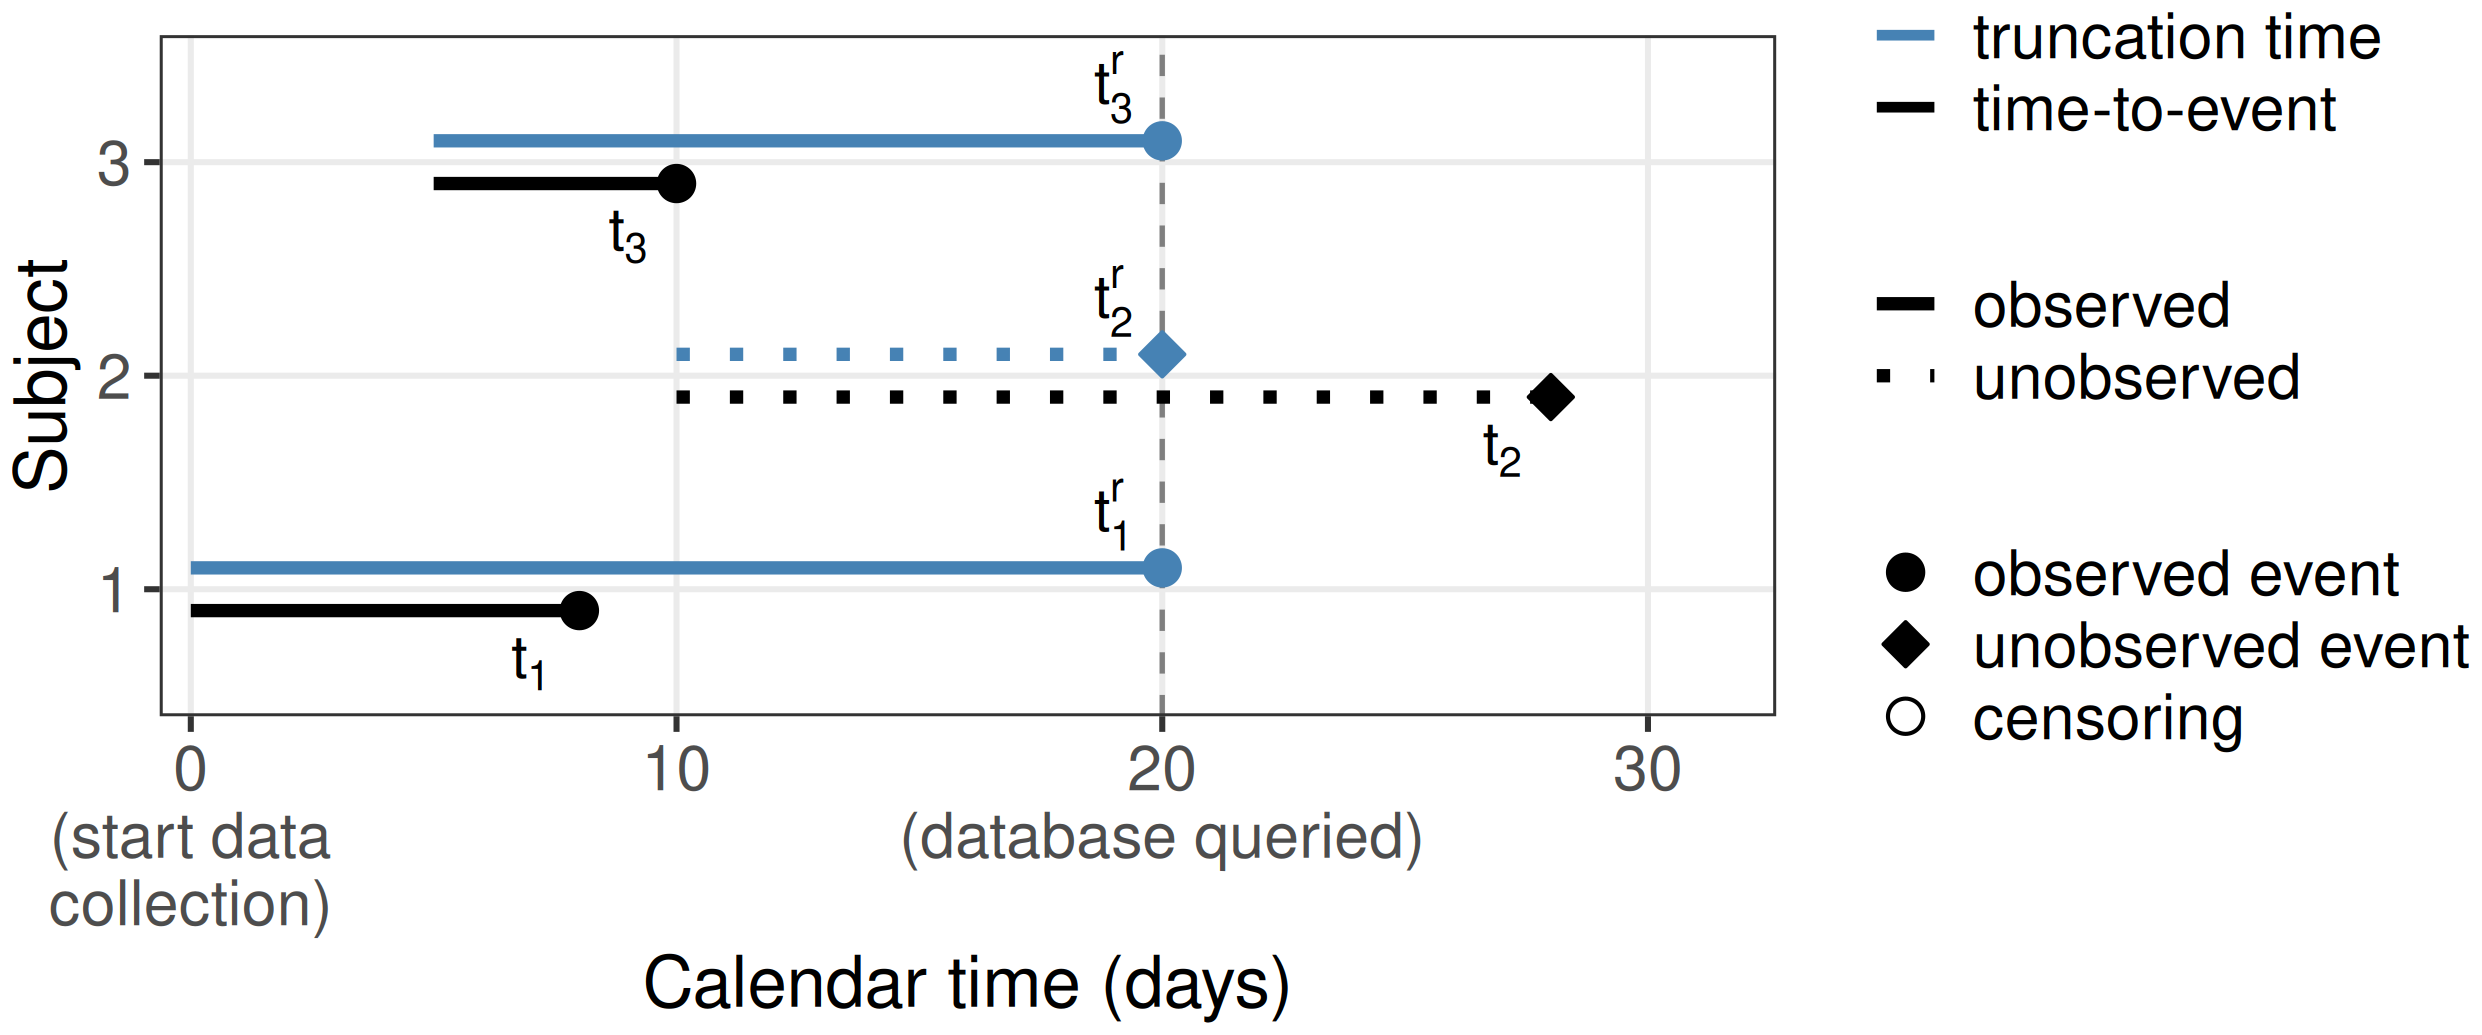
\includegraphics[width=1\linewidth,height=\textheight,keepaspectratio]{Figures/survival/fig-p1c4-right-truncation.png}

}

\caption{\label{fig-p1c4-right-truncation}Illustration of
right-truncation for three subjects observed retrospectively from a
disease registry. The x-axis is calendar time and subjects are recruited
at staggered times (subject 1 at \(\tau = 0\), subject 3 at
\(\tau = 5\), subject 2 at \(\tau = 10\)). For each subject, the upper
steel blue bar runs from recruitment to the database query date
(truncation time, \(t_i^r\)) and the lower black bar runs from
recruitment to the event (\(t_i\)). Subjects 1 and 3 have
\(t_i < t_i^r\) (event before query) and are included in the registry
(solid bars, truncation bar ending in a filled steel blue circle).
Subject 2 has \(t_2 > t_2^r\) (event after query), so they are absent
from the registry. The vertical dashed line marks the database-query
date.}

\end{figure}%

As for left-truncation\index{truncation!left}, ignoring right-truncation
will lead to biased estimates. While for left-truncated data simple
adjustments of the risk set\index{risk set} (see
Section~\ref{sec-non-param-lt}) work for non- and semi-parametric
methods (see Chapter~\ref{sec-classical} for example), this is not the
case for right-truncated data. However, parametric methods can be
employed (see Section~\ref{sec-surv-estimation}) and generalized product
limit estimators for right-truncated data exist (Michael G. Akritas and
LaValley 2005).

\section{Estimation}\label{sec-surv-estimation}

While model-specific algorithms for estimation and prediction are given
in Part IV, there are general concepts that can apply across a wide
range of models. These are separated below between parametric
(Section~\ref{sec-surv-estimation-param}) and non-parametric approaches
(Section~\ref{sec-surv-estimation-non-param}).

\subsection{Parametric estimation}\label{sec-surv-estimation-param}

Consider for now uncensored data \((t_i, \delta_i=1), i=1,\ldots,n\),
where \(t_i\) is the observed realization of the random variable
\(Y_i\). A standard parametric approach\index{parametric estimator}
assumes \(Y_i \stackrel{iid}{\sim} F_Y\) for \(i=1,\ldots,n\), where
\(F_Y\) is a suitable parametric family with finite-dimensional
parameter \(\boldsymbol{\theta}\in \Theta \subseteq \mathbb{R}^d\). When
the parameter dependence matters explicitly (for example, inside a
likelihood), one denotes the cumulative distribution
function\index{cumulative distribution function},
density\index{probability density function}, and survival
function\index{survival function} evaluated at \(\tau\) as
\(F_Y(\tau\mid\boldsymbol{\theta})\),
\(f_Y(\tau\mid\boldsymbol{\theta})\), and
\(S_Y(\tau\mid\boldsymbol{\theta})\). The likelihood of the data is
then\index{likelihood},

\begin{equation}\phantomsection\label{eq-likelihood}{
\mathcal{L}(\boldsymbol{\theta}) = \prod_{i=1}^{n}f_Y(t_i \mid \boldsymbol{\theta}).
}\end{equation}

The corresponding estimation principle is \emph{maximum likelihood
estimation (MLE)}\index{maximum likelihood estimator}, where parameters
are chosen to maximize the probability of the observed data under the
model,

\[
\hat{\boldsymbol{\theta}} = \mathop{\mathrm{arg\,max}}_{\boldsymbol{\theta}} \mathcal{L}(\boldsymbol{\theta}).
\]

In machine learning\index{machine learning}, models are typically
trained by minimizing a loss function\index{loss function} and hence the
negative log-likelihood\index{negative log-likelihood},
\(-\log \mathcal{L}(\boldsymbol{\theta})\), is the loss of an
MLE-trained probabilistic model.

However, in the presence of censoring (\ref{eq-likelihood}) is incorrect
as the exact event time is only known for some subjects. For example,
for right-censored data, it is only known that if the event occurs, it
occurs after the censoring time \(t_i\) and hence the likelihood
contribution for such data points is \(\Pr(Y_i > t_i) = S_Y(t_i)\).

Let \(\mathcal{O}= \{i:\delta_i = 1\}\) be the index set of observed
event times and \(\mathcal{RC} = \{i:\delta_i = 0\}\) the index set of
censored observations. The likelihood of this data can be written as

\begin{equation}\phantomsection\label{eq-right-censoring-likelihood}{
\begin{aligned}
\mathcal{L}(\boldsymbol{\theta})
  & \propto \prod_{i \in \mathcal{O}}f_Y(t_i \mid \boldsymbol{\theta})\prod_{i \in \mathcal{RC}}S_Y(t_i \mid \boldsymbol{\theta})\\
  & = \prod_{i=1}^n f_Y(t_i \mid \boldsymbol{\theta})^{\delta_i}S_Y(t_i \mid \boldsymbol{\theta})^{1-\delta_i}\\
  & = \prod_{i=1}^n \frac{f_Y(t_i \mid \boldsymbol{\theta})^{\delta_i}}{S_Y(t_i \mid \boldsymbol{\theta})^{\delta_i}}S_Y(t_i \mid \boldsymbol{\theta})\\
  & = \prod_{i=1}^n h_Y(t_i \mid \boldsymbol{\theta})^{\delta_i}S_Y(t_i \mid \boldsymbol{\theta}),
\end{aligned}
}\end{equation}

where the last equality follows from (\ref{eq-continuous-hazard}).
Equivalently, training a model on right-censored data by minimizing the
negative log of (\ref{eq-right-censoring-likelihood}) is the MLE view of
the same objective.

Similar adjustments to the likelihood can be made for other types of
censoring and in the presence of
truncation\index{censoring}\index{truncation}. Let \(\mathcal{C}_i\)
denote the event-time information implied by the observed censoring
pattern, such that the likelihood contribution of subject \(i\) is given
by (Klein and Moeschberger 2003),

\begin{equation}\phantomsection\label{eq-likelihood-censoring}{
\Pr(\mathcal{C}_i \mid \boldsymbol{\theta}) =
\begin{cases}
f_Y(t_i \mid \boldsymbol{\theta}),  & \text{observed event}, \\
\Pr(Y_i > t_i \mid \boldsymbol{\theta}) = S_Y(t_i \mid \boldsymbol{\theta}),  & \text{right-censoring}, \\
\Pr(Y_i < t_i \mid \boldsymbol{\theta}) = F_Y(t_i \mid \boldsymbol{\theta}),  & \text{left-censoring}, \\
\Pr(l_i < Y_i \leq r_i \mid \boldsymbol{\theta}) = S_Y(l_i \mid \boldsymbol{\theta}) - S_Y(r_i \mid \boldsymbol{\theta}),  & \text{interval-censoring},
\end{cases}
}\end{equation}

where \(l_i < r_i\) are the interval censoring times
(Section~\ref{sec-types-of-censoring-notation}).

Depending on which of the above contributions occur in the dataset, the
likelihood can be constructed accordingly. Let
\(\mathcal{O}, \mathcal{RC}, \mathcal{LC}, \mathcal{IC}\) be
non-overlapping subsets of the observed data \(\mathcal{D}\) for
subjects with observed event times, right-censoring, left-censoring and
interval-censoring,
respectively\index{censoring!right}\index{censoring!left}\index{censoring!interval}.
Assuming independence between observations and in the absence of
truncation, the likelihood for the observed data can be defined as,

\begin{equation}\phantomsection\label{eq-objective-function}{
\mathcal{L}(\boldsymbol{\theta}) \propto \prod_{i \in \mathcal{O}}f_Y(t_i \mid \boldsymbol{\theta}) \prod_{i \in \mathcal{RC}}S_Y(t_i \mid \boldsymbol{\theta}) \prod_{i \in \mathcal{LC}}F_Y(t_i \mid \boldsymbol{\theta})\prod_{i \in \mathcal{IC}}(S_Y(l_i \mid \boldsymbol{\theta})-S_Y(r_i \mid \boldsymbol{\theta})).
}\end{equation}

In practice, datasets will often not contain all types of censoring, in
which case (\ref{eq-objective-function}) will only contain a subset of
the product terms. This has been illustrated in
(\ref{eq-right-censoring-likelihood}) where
\(\mathcal{LC}=\mathcal{IC}=\emptyset\).

In case of truncation\index{truncation}, the likelihood contribution is
conditioned on inclusion in the observation window,

\begin{equation}\phantomsection\label{eq-likelihood-combined}{
\mathcal{L}_i(\boldsymbol{\theta}) \propto \Pr(\mathcal{C}_i \mid \mathcal{T}_i, \boldsymbol{\theta}) = \frac{\Pr(\mathcal{C}_i \cap \mathcal{T}_i \mid \boldsymbol{\theta})}{\Pr(\mathcal{T}_i \mid \boldsymbol{\theta})},
}\end{equation}

where \(\mathcal{C}_i\) is as defined in (\ref{eq-likelihood-censoring})
and \(\mathcal{T}_i\) is the truncation condition, such that

\begin{equation}\phantomsection\label{eq-likelihood-truncation}{
\Pr(\mathcal{T}_i \mid \boldsymbol{\theta}) =
\begin{cases}
\Pr(Y_i \geq t_i^\ell \mid \boldsymbol{\theta}) = S_Y(t_i^\ell \mid \boldsymbol{\theta}), & \text{left truncation}, \\
\Pr(Y_i \leq t_i^r \mid \boldsymbol{\theta}) = F_Y(t_i^r \mid \boldsymbol{\theta}), & \text{right truncation}.
\end{cases}
}\end{equation}

The conditional contribution in (\ref{eq-likelihood-combined}) rests on
an assumption of \emph{independent
truncation}\index{truncation!independent}: the truncation time is
independent of the event time \(Y_i\), in the same spirit as the
independent-censoring assumption discussed above. This is what justifies
using the marginal event-time distribution in
(\ref{eq-likelihood-truncation}) and treating the truncation bound as
fixed; if the truncation time itself depended on \(Y_i\), conditioning
on inclusion would no longer remove the resulting selection bias.

In almost all settings encountered in practice, combining
(\ref{eq-likelihood-censoring}) and (\ref{eq-likelihood-truncation})
simplifies (\ref{eq-likelihood-combined}) to:

\[
\mathcal{L}_i(\boldsymbol{\theta}) = \frac{\Pr(\mathcal{C}_i \mid \boldsymbol{\theta})}{\Pr(\mathcal{T}_i \mid \boldsymbol{\theta})},
\]

that is, the censoring contribution divided by the probability of being
included in the sample. This holds whenever every event time consistent
with the observed censoring pattern already falls within the truncation
window, as is the case for the common combinations such as
left-truncated, right-censored data. The simplification only breaks down
for a few unusual pairings, for example left-censored \emph{and}
left-truncated observations, where the censored region extends beyond
the truncation boundary; the contribution must then be obtained from the
overlap
\(\Pr(\mathcal{C}_i \cap \mathcal{T}_i \mid \boldsymbol{\theta})\) in
(\ref{eq-likelihood-combined}). Such cases are rarely encountered.

\subsection{Non-parametric
estimation}\label{sec-surv-estimation-non-param}

As the name suggests, non-parametric estimation
\index{non-parametric estimator} techniques do not make (strong)
assumptions about the underlying distribution of event times.

A common principle for such techniques is to partition the follow-up
into intervals (or to define specific time points during the follow-up)
and to estimate the continuous (\ref{eq-continuous-hazard}) or
discrete-time (\ref{eq-discrete-hazard}) hazards for each interval/time
point. Once the respective hazard estimates are obtained, estimates of
other quantities, for example the survival probability, can be derived
based on the relationships in Section~\ref{sec-distributions-continuous}
and Section~\ref{sec-distributions-discrete}.

\subsubsection{Kaplan-Meier estimator}\label{sec-surv-km}

The \emph{Kaplan-Meier (KM) estimator}\index{Kaplan-Meier estimator}
(Kaplan and Meier 1958) is the standard non-parametric estimator of the
survival function (\ref{eq-surv-prob}) under marginally independent
right-censoring. The construction below is a concrete instance of the
hazard-to-survival principle and can be motivated from a discrete-time
perspective. Recall from (\ref{eq-unique-ordered-event-times}) the
definition of unique, ordered, event time \(t_{(k)}, k=1,\ldots,m\).
Define \(\tilde{Y} = k \Leftrightarrow Y \in [t_{(k)},t_{(k+1)})\) as
the discrete-time representation of \(Y\) (with \(t_{(m+1)}\) being some
time point larger than the last event time). Using the quantities
introduced in Section~\ref{sec-data-rc}, the discrete-time
hazard\index{hazard function} (\ref{eq-discrete-hazard}) is estimated as
the ratio of the number of events occurring at \(t_{(k)}\)
(\ref{eq-risk-set-d}) to the number of subjects at risk at \(t_{(k)}\)
(\ref{eq-risk-set-n}),

\begin{equation}\phantomsection\label{eq-disc-haz-non-param}{
h_{\tilde{Y}}(k) = \Pr\left(Y\in [t_{(k)},t_{(k+1)}) \mid Y \geq t_{(k)}\right)=\frac{d_{t_{(k)}}}{n_{t_{(k)}}}.
}\end{equation}

The survival probability\index{survival function} and the definition of
the Kaplan-Meier estimator (\ref{eq-km}) follow from
(\ref{eq-discrete-surv-prob}),

\begin{equation}\phantomsection\label{eq-km}{
S_{KM}(\tau) = \prod_{k:t_{(k)} \leq \tau}\left(1-\frac{d_{t_{(k)}}}{n_{t_{(k)}}}\right),
}\end{equation}

which is a step-function at the observed ordered event times
\(t_{(k)}, k=1,\ldots,m\), with
\(S_{KM}(\tau) = 1\ \forall \tau < t_{(1)}\). The estimator is usually
constructed to estimate survival probabilities at all unique event
times. In this book, \(\hat{S}_{KM}\) specifically refers to the
Kaplan-Meier estimator fit on some training data.

The variance of the Kaplan-Meier estimator is commonly estimated using
the asymptotically consistent Greenwood estimator (Greenwood
1926)\index{Kaplan-Meier estimator!Greenwood}:

\begin{equation}\phantomsection\label{eq-greenwood}{
\widehat{\operatorname{Var}}(S_{KM}(\tau)) = S_{KM}^2(\tau) \sum_{k:t_{(k)} \leq \tau} \frac{d_{t_{(k)}}}{n_{t_{(k)}}(n_{t_{(k)}} - d_{t_{(k)}})}.
}\end{equation}

For illustration, consider the \texttt{tumor} dataset from
Section~\ref{sec-data-rc}. Figure~\ref{fig-p1c4-km-tumor} shows the
estimated survival probability obtained by applying the Kaplan-Meier
estimator to the full dataset, containing observations of \(n=776\)
subjects. By definition, the survival function starts at \(S(\tau)=1\)
at \(\tau=0\) and monotonically decreases toward \(S(\tau)=0\) for
\(\tau \rightarrow \infty\). However, follow-ups are usually not
infinite and in the presence of censoring, the survival function may not
reach 0 by the end of the observation period. For the Kaplan-Meier
estimator specifically, \(\hat{S}_{KM}(t_{(m)}) = 0\) only if there are
no censored observations at the last observed outcome time, or
equivalently, \(d_{t_{(m)}} = n_{t_{(m)}}\).

Dotted lines in Figure~\ref{fig-p1c4-km-tumor} indicate the median
survival\index{median survival time}, defined as the time at which the
survival function reaches \(S(\tau) = 0.5\). In this example, the median
survival time is approximately 1,500 days, which means 50\% of the
subjects are expected to die within 1,500 days of the operation.

\begin{figure}

\centering{

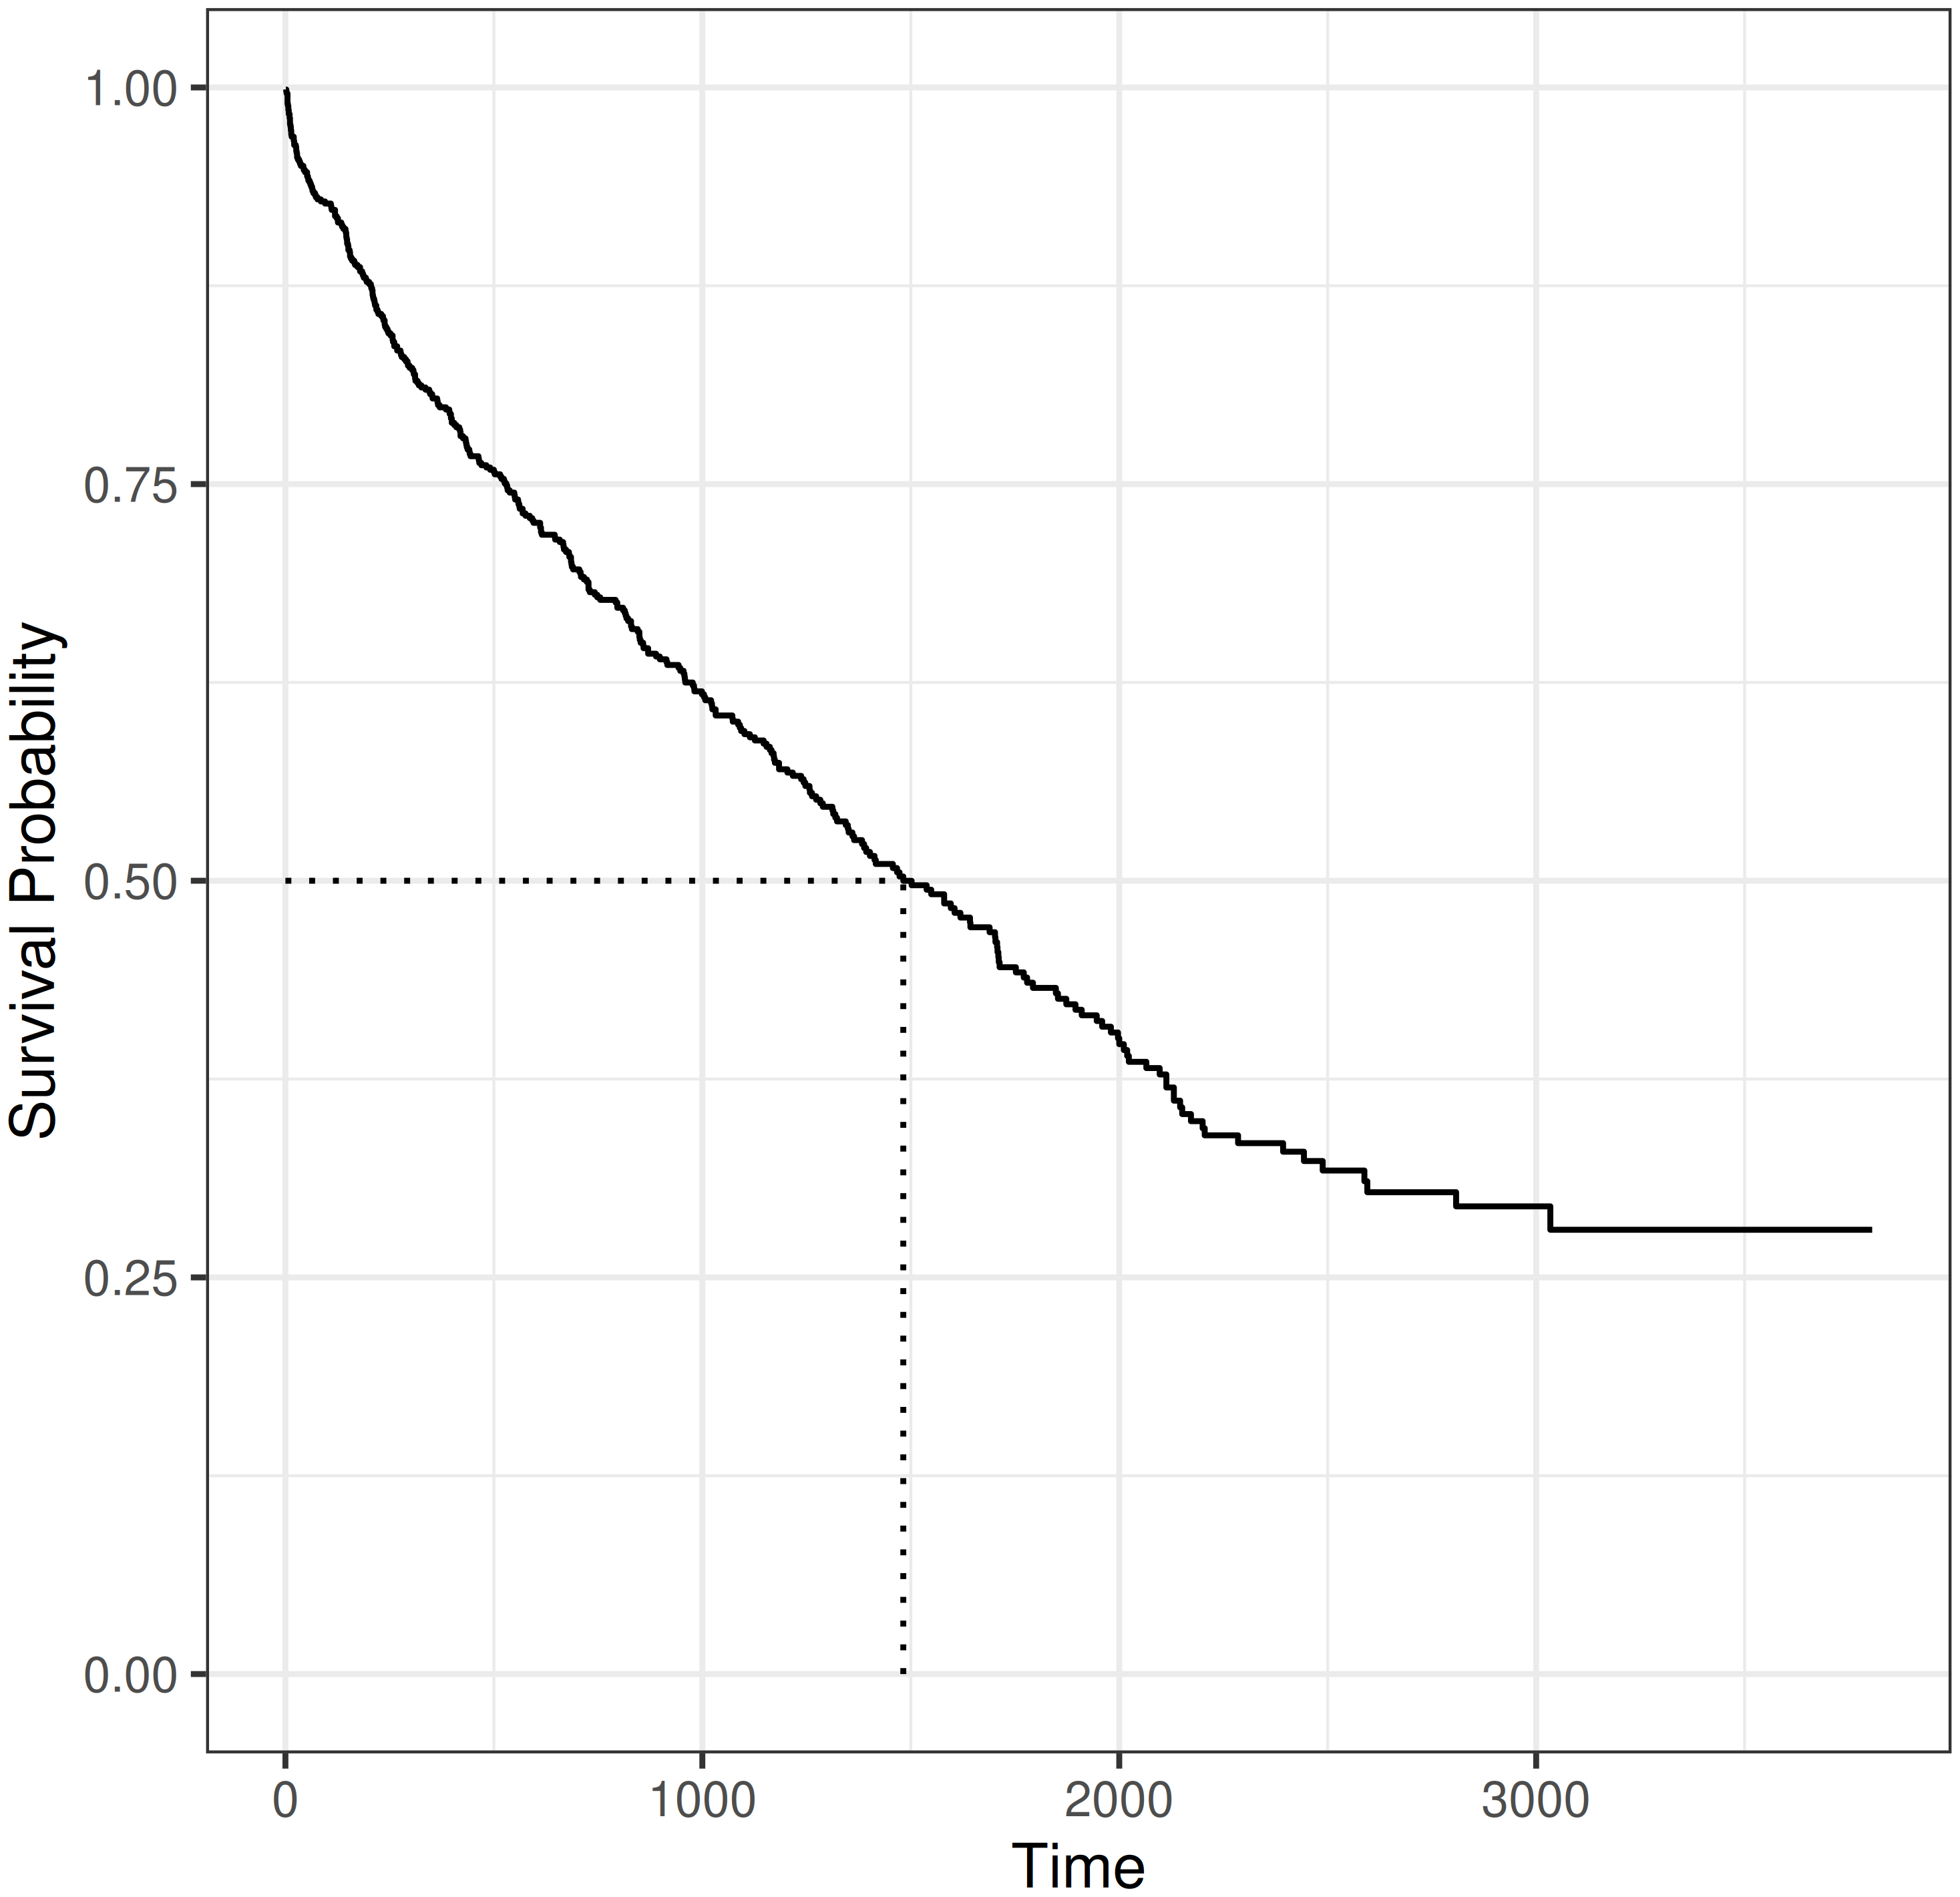
\includegraphics[width=0.6\linewidth,height=\textheight,keepaspectratio]{Figures/survival/fig-p1c4-km-tumor.png}

}

\caption{\label{fig-p1c4-km-tumor}Kaplan-Meier estimate for the
\texttt{tumor} data (Bender and Scheipl 2018). The estimated survival
probabilities are given by the solid step-function. Dotted lines
indicate the median survival time.}

\end{figure}%

While the Kaplan-Meier estimator does not directly support estimation of
covariate effects on the estimated survival probabilities, it is often
used for descriptive analysis by applying the estimator to different
subgroups (referred to as stratification\index{stratification} in
survival analysis). For example, Figure~\ref{fig-p1c4-km-age-bin-tumor}
shows \(\hat{S}_{KM}\) curves for subjects aged 50 years or older and
subjects younger than 50 years. Dashed lines again illustrate median
survival times; in this example, the median survival time does not exist
for the younger age group as their estimated survival function does not
cross \(0.5\).

\begin{figure}

\centering{

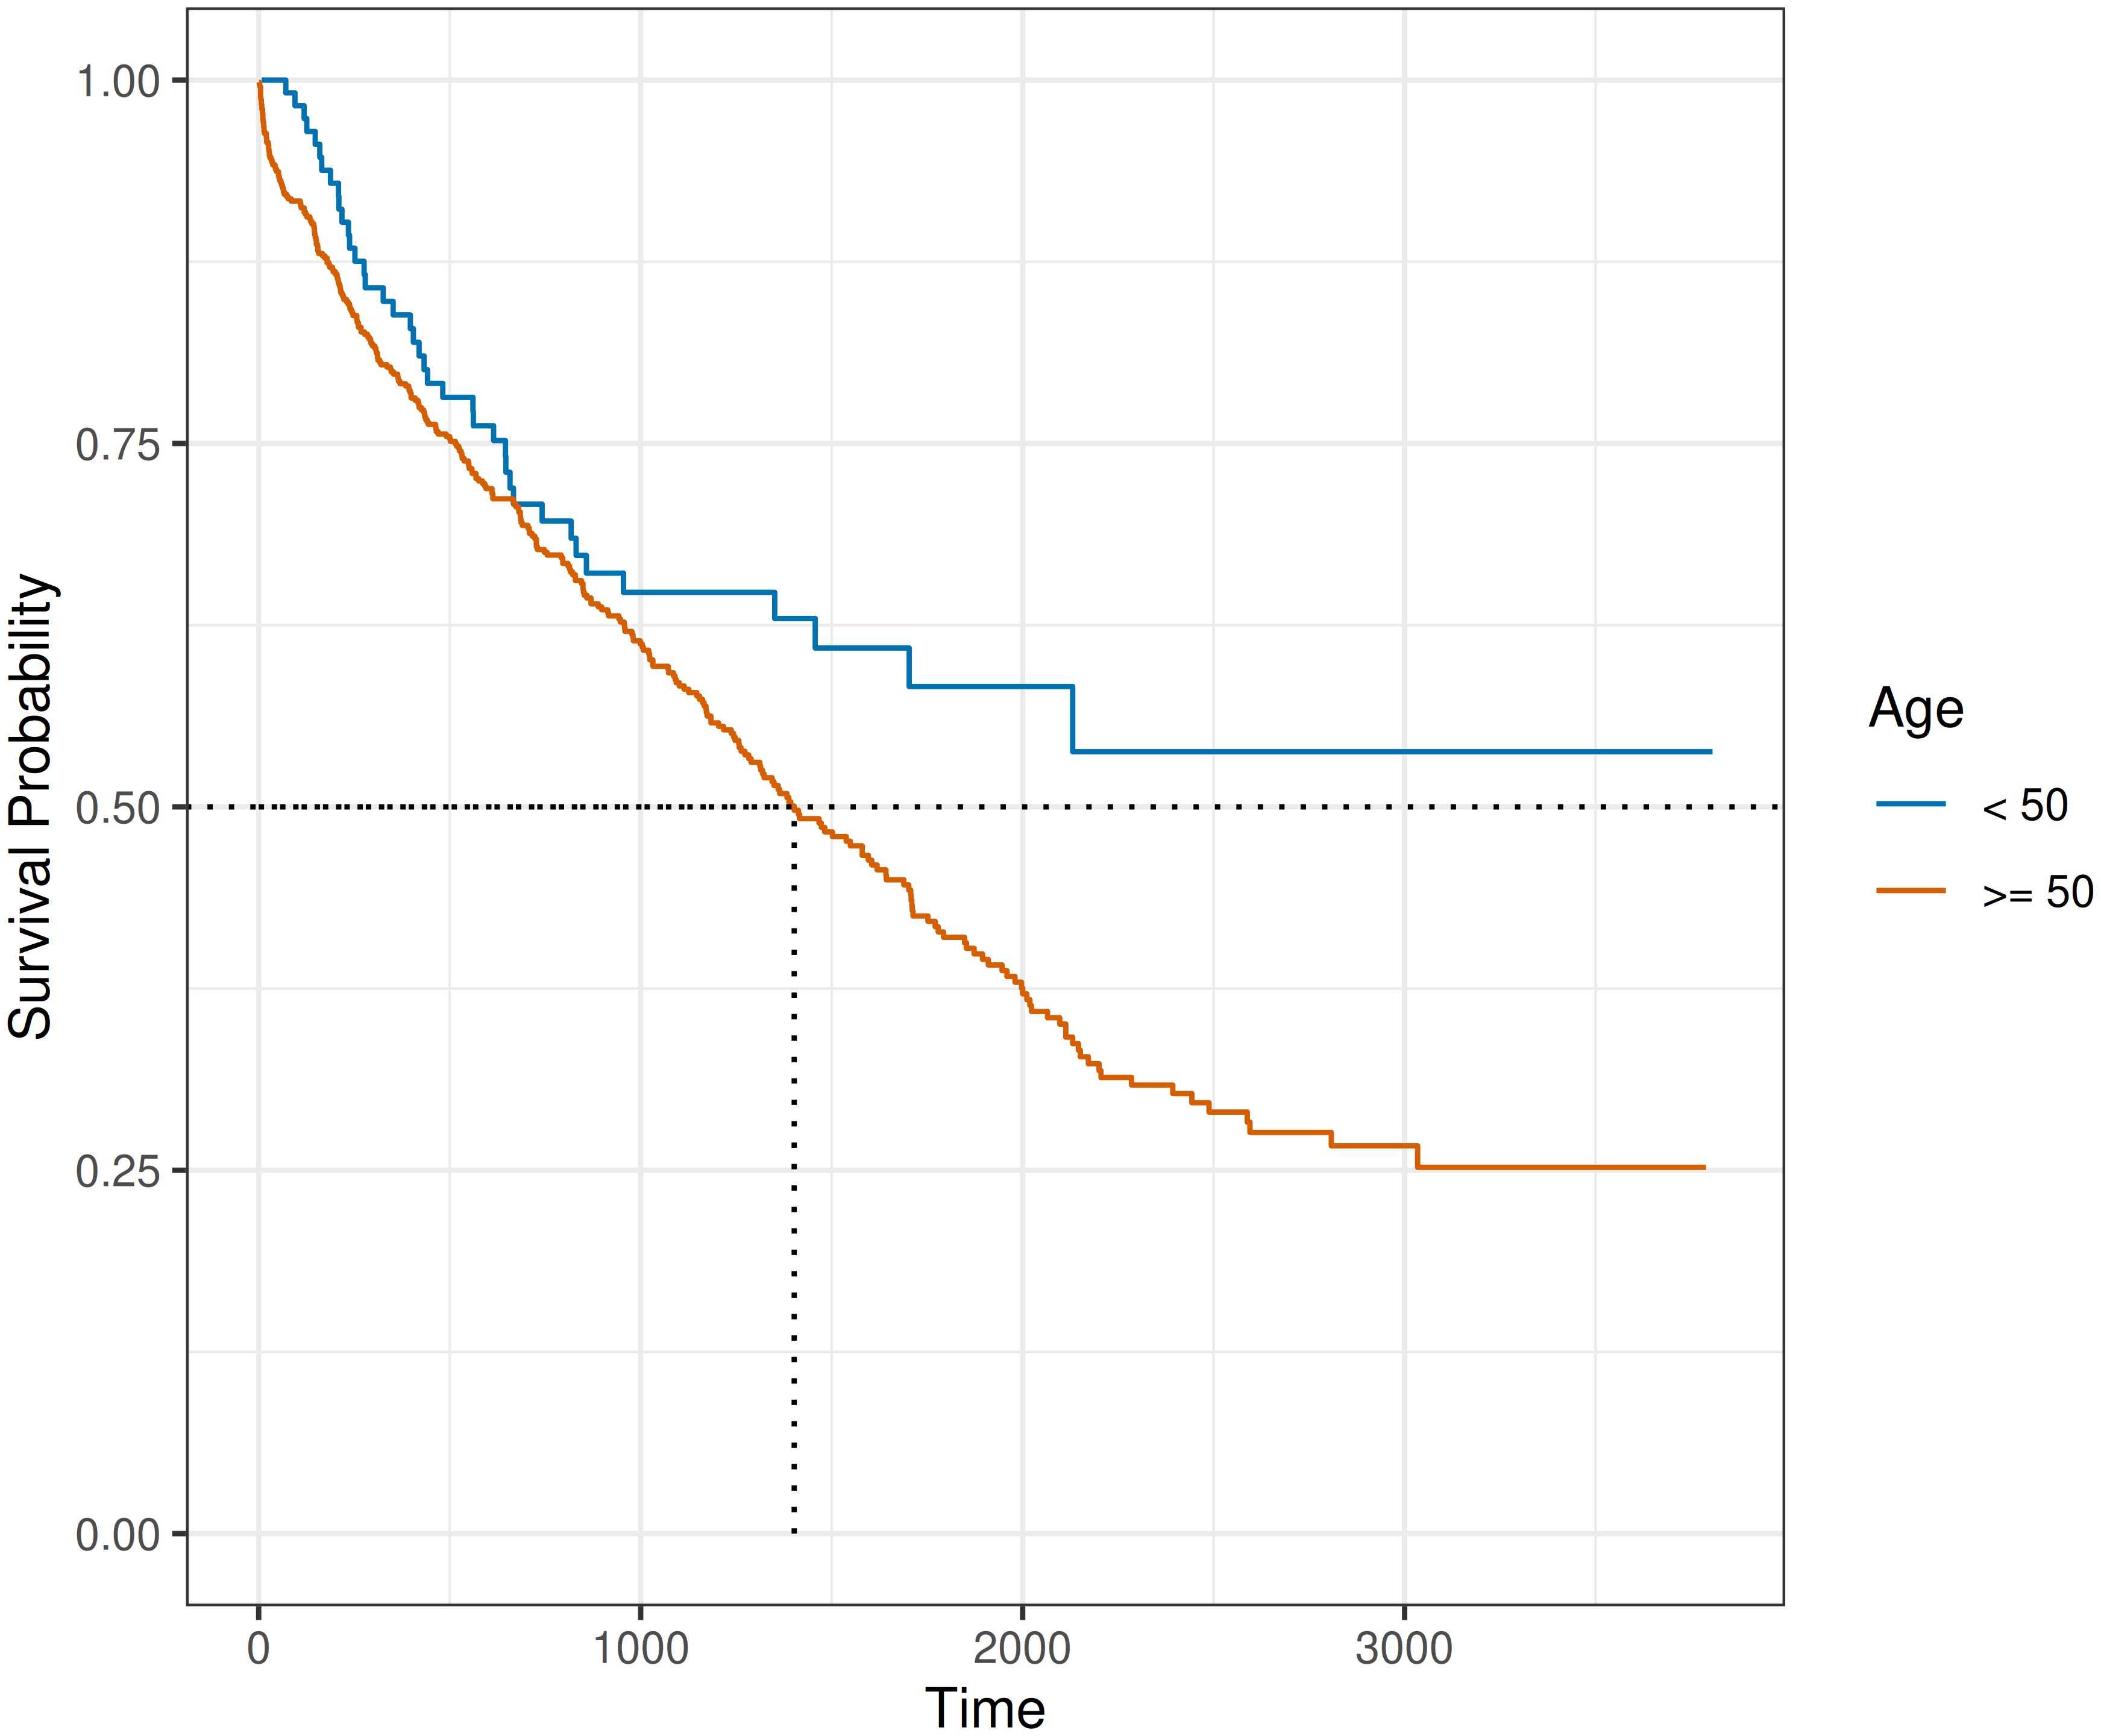
\includegraphics[width=0.7\linewidth,height=\textheight,keepaspectratio]{Figures/survival/fig-p1c4-km-age-bin-tumor.png}

}

\caption{\label{fig-p1c4-km-age-bin-tumor}Kaplan-Meier estimate for the
\texttt{tumor} data (Bender and Scheipl 2018) applied to subgroups of
subjects of 50 or more years old and less than 50 years old,
respectively. The estimated survival probabilities are given by the
solid step-function. Dotted lines indicate the median survival time.}

\end{figure}%

\subsubsection{Nelson-Aalen}\label{sec-surv-na}

Another popular non-parametric estimator is the
Nelson-Aalen\index{Nelson-Aalen estimator} estimator (Aalen 1978; Nelson
1972), which is based on the empirical discrete-time hazards estimator
(\ref{eq-disc-haz-non-param}). Rather than estimating the survival
probability, the Nelson-Aalen estimator estimates the cumulative hazard
function\index{cumulative hazard function} as,

\begin{equation}\phantomsection\label{eq-nelson-aalen}{
H_{NA}(\tau) = \sum_{k:t_{(k)}\leq \tau} h_{\tilde{Y}}(t_{(k)}) = \sum_{k:t_{(k)}\leq \tau} \frac{d_{t_{(k)}}}{n_{t_{(k)}}}.
}\end{equation}

This definition implies that if \(\tau\) falls between two unique event
times, then \(H_{NA}(\tau)\) equals the value of the estimate at the
most recent event time:

\[
H_{NA}(\tau) = H_{NA}(t_{(k)})\ \forall \tau \in [t_{(k)}, t_{(k+1)}).
\]

Using (\ref{eq-surv-haz}), a survival probability estimator based on the
Nelson-Aalen estimator can be defined as,

\begin{equation}\phantomsection\label{eq-surv-na}{
S_{NA}(\tau) = \exp(-H_{NA}(\tau)).
}\end{equation}

Kaplan--Meier\index{Kaplan-Meier estimator} and Nelson--Aalen are
consistent for survival and cumulative hazard respectively under
independent right-censoring. Both of these non-parametric estimators can
be used as simple predictive methods
(Section~\ref{sec-classical-nonpar}), and are often used as informative
baseline models\index{baseline model}, which can be compared to
sophisticated alternatives to improve
interpretability\index{model interpretability} in model evaluation
(Herrmann et al. 2021; Huang et al. 2020; P. Wang, Li, and Reddy 2019).
Both methods can also be used for graphical
calibration\index{calibration} of models (Section~\ref{sec-calib-km})
and other diagnostic graphical tools (Habibi et al. 2018; Jager et al.
2008; Moghimi-dehkordi et al. 2008).

\subsubsection{Left truncation}\label{sec-non-param-lt}

Non- and semi-parametric estimators can be easily extended to deal with
left-truncation\index{truncation!left} by adjusting the risk
set\index{risk set} definition (\ref{eq-risk-set}) to the more general
definition (McGough et al. 2021),

\begin{equation}\phantomsection\label{eq-risk-lt}{
\mathcal{R}_\tau^\ell = \{i: t_i^\ell \ \leq \tau \leq t_i \}, 
}\end{equation}

where \(t_i, t_i^\ell\) are the outcome time and left-truncation time of
observation \(i\) respectively. This definition excludes individuals
from the risk set until their left-truncation time has occurred.

The number of individuals at risk at \(\tau\) is then the cardinality of
(\ref{eq-risk-lt}),

\[
n^\ell_\tau = \vert \mathcal{R}_\tau^\ell \vert = \sum_i \mathbb{I}(t_i^\ell \leq \tau \leq t_i).
\]

The Kaplan-Meier\index{Kaplan-Meier estimator} (\ref{eq-km}) and
Nelson-Aalen\index{Nelson-Aalen estimator} (\ref{eq-nelson-aalen})
estimators can be used by replacing \(n_{t_{(k)}}\) with
\(n^\ell_{t_{(k)}}\); \(d_{t_{(k)}}\) is calculated as usual.

For illustration, consider an excerpt from the infants data in
Table~\ref{tbl-surv-data-infants} discussed in
Section~\ref{sec-left-truncation}, where \(t\) is the observed event or
censoring time and \(t^\ell\) is the left-truncation time.

\begin{longtable}[]{@{}rrrrrl@{}}
\caption{Excerpt of the \texttt{infants} (Broström 2024) time-to-event
dataset. Rows are individual observations (id), \texttt{group} indicates
matched infants, \(t^\ell\) is the left-truncation time (time of
inclusion into the study), \(t\) is the observed time, \(\delta\) is the
event indicator.}\label{tbl-surv-data-infants}\tabularnewline
\toprule\noalign{}
group & id & \(t^\ell\) & \(t\) & \(\delta\) & mother \\
\midrule\noalign{}
\endfirsthead
\toprule\noalign{}
group & id & \(t^\ell\) & \(t\) & \(\delta\) & mother \\
\midrule\noalign{}
\endhead
\bottomrule\noalign{}
\endlastfoot
1 & 1 & 55 & 365 & 0 & dead \\
1 & 2 & 55 & 365 & 0 & alive \\
1 & 3 & 55 & 365 & 0 & alive \\
2 & 4 & 13 & 76 & 1 & dead \\
2 & 5 & 13 & 365 & 0 & alive \\
2 & 6 & 13 & 365 & 0 & alive \\
4 & 7 & 2 & 16 & 1 & dead \\
4 & 8 & 2 & 365 & 0 & alive \\
4 & 9 & 2 & 365 & 0 & alive \\
\end{longtable}

In Table~\ref{tbl-surv-data-infants}, without stratifying according to
mother's status, the first observed event time is \(t_{(1)} = t_7=16\).
Then, ignoring left-truncation,

\begin{itemize}
\tightlist
\item
  \(\mathcal{R}_{t_{(1)}} = \{1,2,3,4,5,6,7,8,9\}\)
\item
  \(d_{t_{(1)}} = 1\)
\item
  \(n_{t_{(1)}} = 9\)
\item
  \(S(t_{(1)}) = 1 - \frac{1}{9} \approx 0.9\)
\end{itemize}

In contrast, when left-truncation is taken into account, subjects only
enter the risk set for the event after their left-truncation time as it
is known they survived until \(t_i^\ell\) so cannot be at risk for the
event before that time. Thus,

\begin{itemize}
\tightlist
\item
  \(\mathcal{R}^\ell_{t_{(1)}} = \{4, 5, 6, 7, 8, 9\}\)
\item
  \(d_{t_{(1)}} = 1\)
\item
  \(n_{t_{(1)}}^\ell = 6\)
\item
  \(S(t_{(1)}) = 1 - \frac{1}{6} \approx 0.8\)
\end{itemize}

In the presence of left-truncation,
\(n_{t_{(k)}}^\ell \leq  n_{t_{(k)}}\) and therefore
\(S^\ell(t_{(k)}) \leq S(t_{(k)})\).

Figure~\ref{fig-p1c4-km-infants} shows the estimated survival
probabilities when left-truncation is ignored (left panel) and when it
is accounted for (right panel). Consistent with
\(S^\ell(t_{(k)}) \leq S(t_{(k)})\), ignoring left-truncation yields
larger survival estimates in both groups. The gap between the curves is
more pronounced for infants whose mother died, so ignoring
left-truncation also understates the effect of the mother's death on
infant survival.

\begin{figure}

\centering{

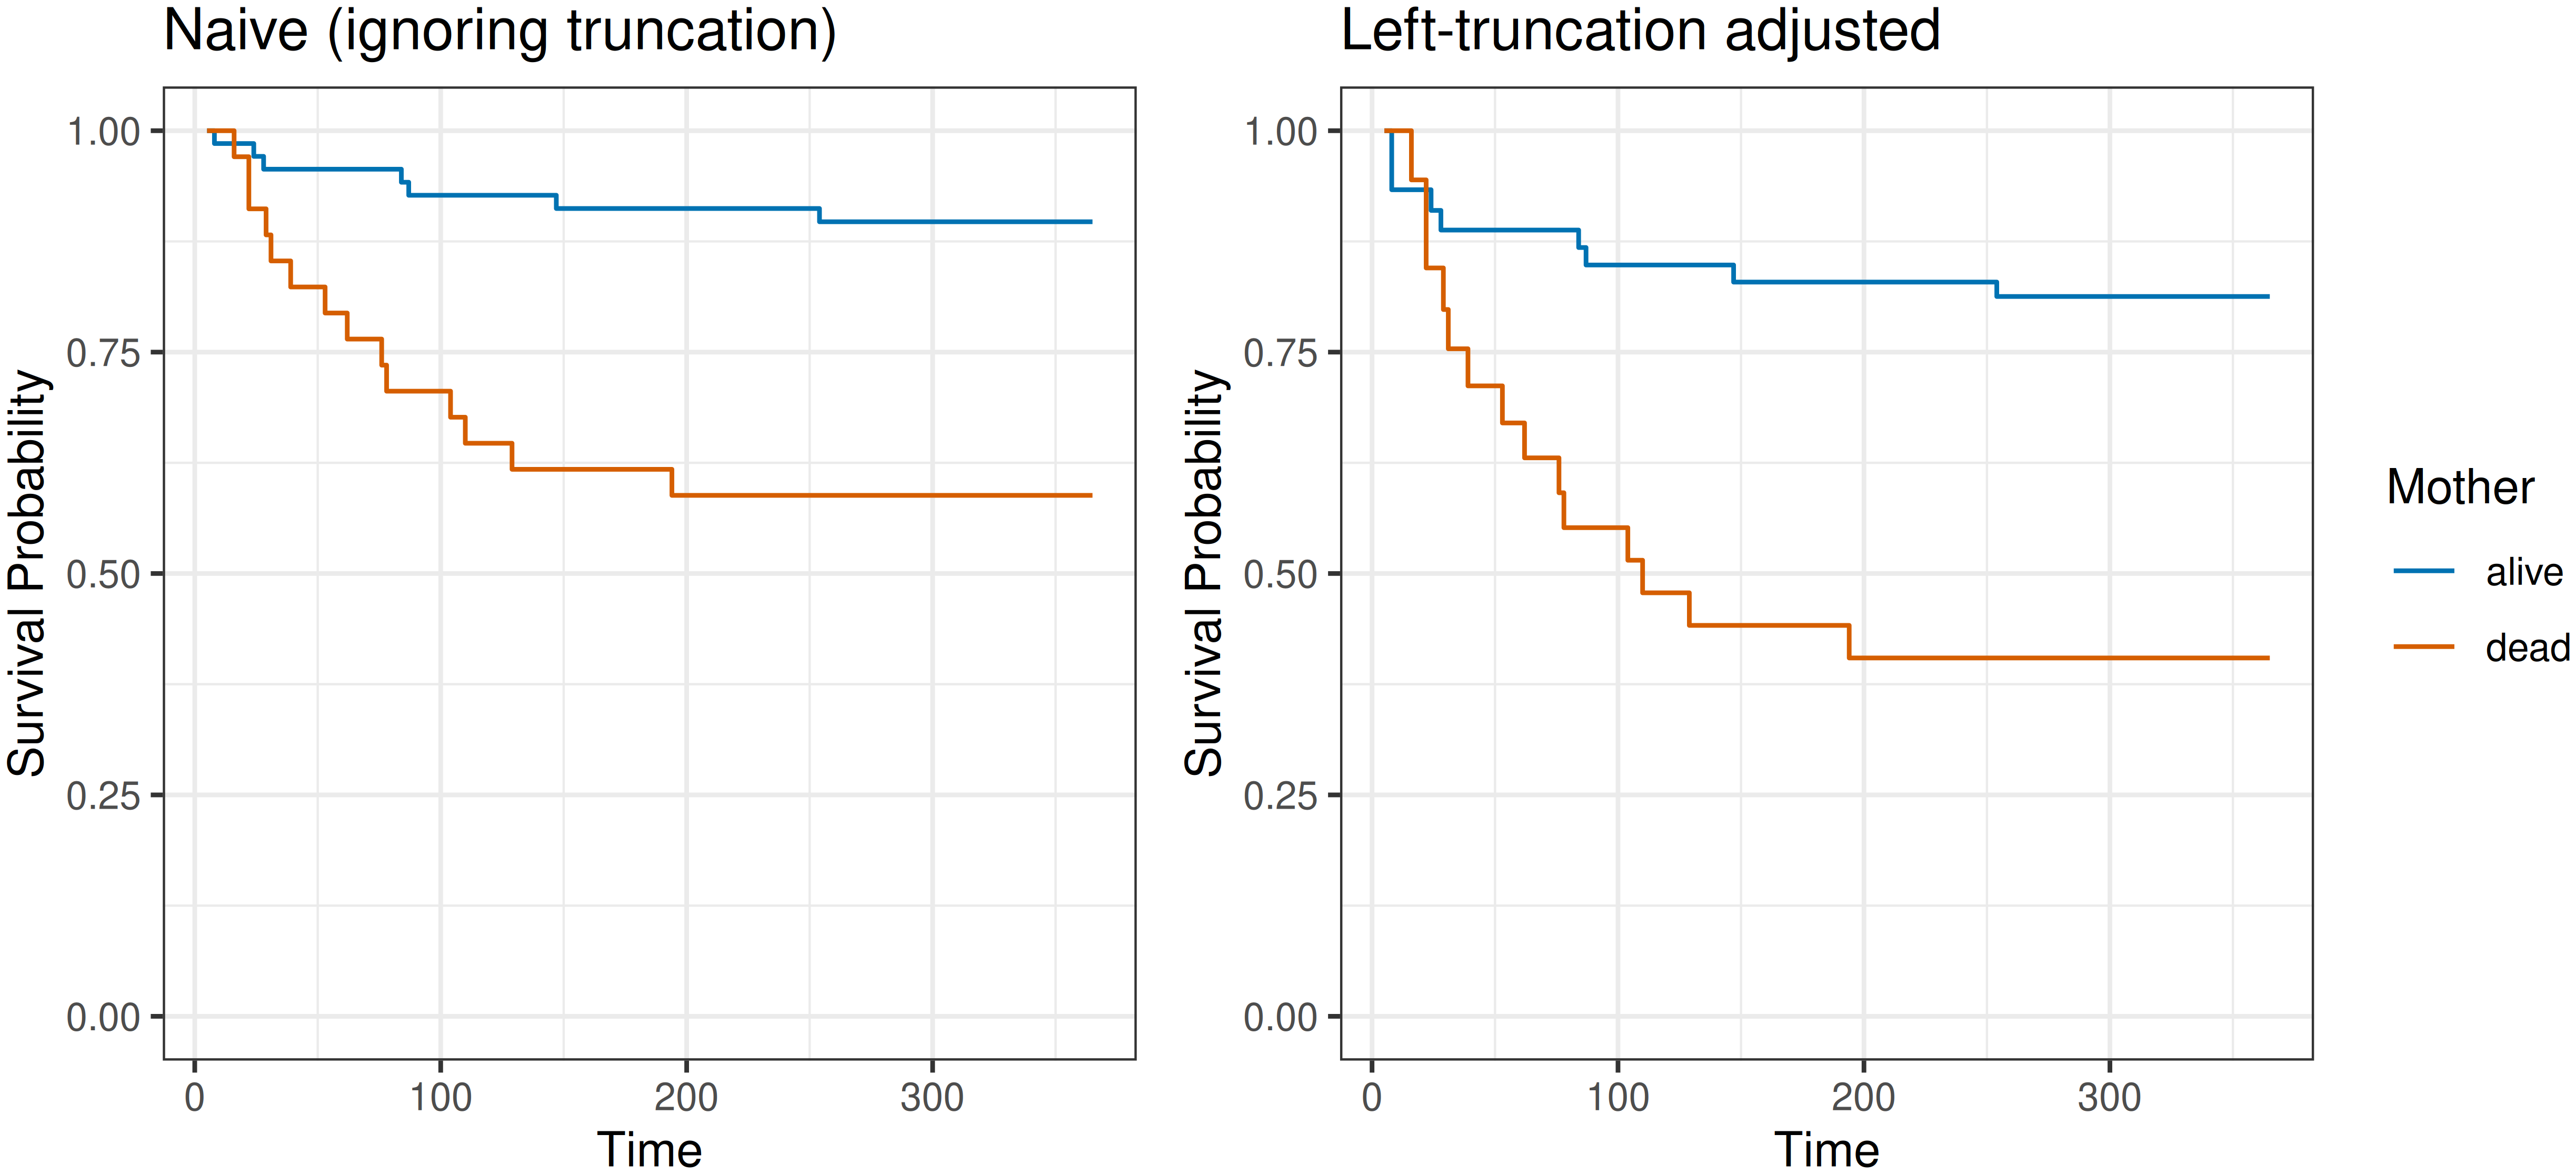
\includegraphics[width=0.9\linewidth,height=\textheight,keepaspectratio]{Figures/survival/fig-p1c4-km-infants.png}

}

\caption{\label{fig-p1c4-km-infants}Left: Kaplan-Meier estimate of
survival probabilities of infants depending on status of the mother
ignoring left-truncation. Right: Kaplan-Meier estimate of survival
probabilities adjusting for left-truncation.}

\end{figure}%

\subsubsection{Interval-censoring}\label{interval-censoring}

For interval-censored\index{censoring!interval} data, the
Kaplan-Meier\index{Kaplan-Meier estimator} estimator is replaced by the
non-parametric maximum likelihood estimator
(NPMLE)\index{non-parametric maximum likelihood estimator} (Sun 2006; Z.
Zhang and Sun 2010). The NPMLE maximizes the likelihood derived in
Section~\ref{sec-surv-estimation-param} under interval-censoring without
assuming a parametric form for \(S_Y\).

Because closed-form maximization is not available, the standard tool is
Turnbull's\index{Turnbull estimator} iterative \emph{self-consistency
algorithm} (Turnbull 1976), a special case of the
expectation-maximization algorithm in which the unobserved exact event
times are treated as latent data. The intuition is that an observation
\(i\) should only contribute to the estimated probability of an event at
a candidate time \(\tau\) if its interval \((L_i, R_i]\) could plausibly
have contained that event.

The idea (Algorithm 1) is to first construct an ordered grid
\(0 = \tau_0 < \tau_1 < \cdots < \tau_m\) by pooling the data's interval
endpoints \(\{0\} \cup \{L_1, R_1, \ldots, L_n, R_n\}\) and dropping
duplicates. The candidate event times are the right endpoints of the
grid intervals \((\tau_{k-1}, \tau_k]\). The NPMLE is a step function on
this grid. Only intervals contained in some observation interval
\((L_i, R_i]\) can carry positive mass (Peto 1973; Turnbull 1976), and
Algorithm 1 assigns zero mass to the rest automatically. Note that the
\(\tau_k\) are \emph{constructed} grid points, distinct from the
observed ordered event times \(t_{(k)}\)
(\ref{eq-unique-ordered-event-times}) used for the right-censored
Kaplan-Meier in Section~\ref{sec-surv-km}. A convenient initial estimate
\(\hat{S}^{0}\) is the \emph{right-endpoint Kaplan-Meier}: for every
observation that is not right-censored (those with finite \(R_i\)), the
right endpoint \(R_i\) of its censoring interval is used as a surrogate
for the unknown event time, and the ordinary Kaplan-Meier estimator is
then applied (Giolo 2004; Turnbull 1974).

\begin{tcolorbox}[enhanced jigsaw, toprule=.15mm, bottomtitle=1mm, opacityback=0, breakable, leftrule=.75mm, title={Algorithm 1 (Turnbull NPMLE for interval-censored data)}, toptitle=1mm, bottomrule=.15mm, colback=white, colframe=quarto-callout-note-color-frame, titlerule=0mm, opacitybacktitle=0.6, coltitle=black, rightrule=.15mm, left=2mm, colbacktitle=quarto-callout-note-color!10!white, arc=.35mm]

\textbf{Inputs:} observed intervals \(\{(L_i, R_i] : i = 1,\ldots,n\}\);
tolerance \(\epsilon\) (default \(10^{-3}\)).

\textbf{Initialization:} construct the grid \(\tau_0 < \cdots < \tau_m\)
from the pooled endpoints. For each subject \(i\) and grid index \(k\),
define the \emph{plausibility indicator}

\[
w_{ik} = \mathbb{I}\bigl((\tau_{k-1}, \tau_k] \subseteq (L_i, R_i]\bigr),
\]

recording whether the \(k\)th grid interval could have contained subject
\(i\)'s event. Initialize \(\hat{S}^{0}(\tau_k), k = 0, \ldots, m\) as
the right-endpoint Kaplan-Meier.

\begin{enumerate}
\def\labelenumi{\arabic{enumi}.}
\tightlist
\item
  \textbf{For} \(j = 1, 2, \ldots\) \textbf{until convergence:}
\item
  ~~~~~For \(k = 1, \ldots, m\), compute the current probability mass on
  the \(k\)th grid interval \((\tau_{k-1}, \tau_k]\):
\end{enumerate}

\[
p_{\tau_k}^{(j)} = \hat{S}^{j-1}(\tau_{k-1}) - \hat{S}^{j-1}(\tau_k).
\]

\begin{enumerate}
\def\labelenumi{\arabic{enumi}.}
\setcounter{enumi}{2}
\tightlist
\item
  ~~~~~For \(k = 1, \ldots, m\), compute the expected number of events
  in \((\tau_{k-1}, \tau_k]\) under the current estimate:
\end{enumerate}

\[
d_{\tau_k}^{(j)} = \sum_{i=1}^{n} \frac{w_{ik}\, p_{\tau_k}^{(j)}}{\sum_{l=1}^{m} w_{il}\, p_{\tau_l}^{(j)}}.
\]

\begin{enumerate}
\def\labelenumi{\arabic{enumi}.}
\setcounter{enumi}{3}
\tightlist
\item
  ~~~~~Compute the corresponding number ``still at risk just before
  \(\tau_k\)'':
\end{enumerate}

\[
n_{\tau_k}^{(j)} = \sum_{l=k}^{m} d_{\tau_l}^{(j)}.
\]

\begin{enumerate}
\def\labelenumi{\arabic{enumi}.}
\setcounter{enumi}{4}
\tightlist
\item
  ~~~~~Plug \(d_{\tau_k}^{(j)}\) and \(n_{\tau_k}^{(j)}\) into the
  Kaplan-Meier formula (\ref{eq-km}) to obtain \(\hat{S}^{j}\).
\item
  ~~~~~\textbf{If}
  \(\max_{k}\bigl\vert \hat{S}^{j}(\tau_k) - \hat{S}^{j-1}(\tau_k)\bigr\vert < \epsilon\),
  \textbf{stop}.
\item
  \textbf{Return} \(\hat{S}^{j}\).
\end{enumerate}

The estimator is constant on each grid interval
\((\tau_{k-1}, \tau_k]\). For plotting it is conventional to display
jumps at the right endpoints \(\tau_k\); some authors instead place each
jump at the midpoint \((\tau_{k-1} + \tau_k)/2\) to reflect the
underlying uncertainty about exact event timing --- both are valid
presentations of the same estimator.

\end{tcolorbox}

For illustration of the initial step of the algorithm, consider three
subjects with intervals \((0, 5]\), \((2, 8]\), and \((4, 10]\). Pooling
the endpoints gives \(\{0, 2, 4, 5, 8, 10\}\), so \(m=5\) and
\(\tau_0 = 0\), \(\tau_1 = 2\), \(\tau_2 = 4\), \(\tau_3 = 5\),
\(\tau_4 = 8\), \(\tau_5 = 10\). The plausibility-indicator matrix
\(\{w_{ik}\}\) from the initialization is in Table~\ref{tbl-turnbull}.
Reading the matrix: subject 1's event could fall in any of the first
three grid intervals (all contained in \((0, 5]\)); the third grid
interval \((4, 5]\) is the only one in which all three subjects' events
could fall.

\begin{longtable}[]{@{}
  >{\raggedright\arraybackslash}p{(\linewidth - 12\tabcolsep) * \real{0.1429}}
  >{\raggedright\arraybackslash}p{(\linewidth - 12\tabcolsep) * \real{0.1429}}
  >{\raggedright\arraybackslash}p{(\linewidth - 12\tabcolsep) * \real{0.1429}}
  >{\raggedright\arraybackslash}p{(\linewidth - 12\tabcolsep) * \real{0.1429}}
  >{\raggedright\arraybackslash}p{(\linewidth - 12\tabcolsep) * \real{0.1429}}
  >{\raggedright\arraybackslash}p{(\linewidth - 12\tabcolsep) * \real{0.1429}}
  >{\raggedright\arraybackslash}p{(\linewidth - 12\tabcolsep) * \real{0.1429}}@{}}
\caption{Plausibility-indicator matrix \(\{w_{ik}\}\) from Turnbull
example.}\label{tbl-turnbull}\tabularnewline
\toprule\noalign{}
\begin{minipage}[b]{\linewidth}\raggedright
subject \(i\)
\end{minipage} & \begin{minipage}[b]{\linewidth}\raggedright
\((L_i, R_i]\)
\end{minipage} & \begin{minipage}[b]{\linewidth}\raggedright
\(w_{i,1}\)
\end{minipage} & \begin{minipage}[b]{\linewidth}\raggedright
\(w_{i,2}\)
\end{minipage} & \begin{minipage}[b]{\linewidth}\raggedright
\(w_{i,3}\)
\end{minipage} & \begin{minipage}[b]{\linewidth}\raggedright
\(w_{i,4}\)
\end{minipage} & \begin{minipage}[b]{\linewidth}\raggedright
\(w_{i,5}\)
\end{minipage} \\
\midrule\noalign{}
\endfirsthead
\toprule\noalign{}
\begin{minipage}[b]{\linewidth}\raggedright
subject \(i\)
\end{minipage} & \begin{minipage}[b]{\linewidth}\raggedright
\((L_i, R_i]\)
\end{minipage} & \begin{minipage}[b]{\linewidth}\raggedright
\(w_{i,1}\)
\end{minipage} & \begin{minipage}[b]{\linewidth}\raggedright
\(w_{i,2}\)
\end{minipage} & \begin{minipage}[b]{\linewidth}\raggedright
\(w_{i,3}\)
\end{minipage} & \begin{minipage}[b]{\linewidth}\raggedright
\(w_{i,4}\)
\end{minipage} & \begin{minipage}[b]{\linewidth}\raggedright
\(w_{i,5}\)
\end{minipage} \\
\midrule\noalign{}
\endhead
\bottomrule\noalign{}
\endlastfoot
1 & \((0, 5]\) & 1 & 1 & 1 & 0 & 0 \\
2 & \((2, 8]\) & 0 & 1 & 1 & 1 & 0 \\
3 & \((4, 10]\) & 0 & 0 & 1 & 1 & 1 \\
\end{longtable}

\section{Estimation of the censoring
distribution}\label{sec-censoring-distribution}

The techniques discussed in Section~\ref{sec-surv-estimation} can also
be used to estimate the distribution of censoring times
\((t_i, 1-\delta_i)\)\index{censoring distribution}. This is useful to
calculate the inverse probability of censoring
weights\index{inverse probability of censoring weights}
(Section~\ref{sec-surv-ipcw}), which are used in the evaluation of
survival models (Section~\ref{sec-cindex}) and to account for
(covariate-)dependent censoring (Willems et al. 2018).

\subsection{The Kaplan-Meier estimator for the censoring
distribution}\label{sec-surv-km-censoring}

To utilize the Kaplan-Meier\index{Kaplan-Meier estimator} estimator
(\ref{eq-km}) to estimate the distribution of censoring times, the
numerator \(d_{\tau}\) is replaced with the number of censoring events
at \(\tau\),

\[
d_\tau^C = \sum_i \mathbb{I}(t_i = \tau, \delta_i = 0).
\]

The Kaplan-Meier estimator for the censoring distribution is then given
by,

\begin{equation}\phantomsection\label{eq-km-censoring}{
G_{KM}(\tau) = \prod_{k:c_{(k)} \leq \tau}\left(1-\frac{d^C_{c_{(k)}}}{n_{c_{(k)}}}\right),
}\end{equation}

where \(c_{(1)} < \cdots < c_{(m_C)}\) denote the unique, ordered
censoring times.

Throughout this book, \(\hat{G}_{KM}\) is used to refer to the
Kaplan-Meier estimator fit to the observed censoring times
\((t_i, 1-\delta_i)\) from some training data.

\subsection{Inverse probability of censoring weights
(IPCW)}\label{sec-surv-ipcw}

A fundamental concept in survival analysis is inverse probability of
censoring (IPC)
weighting\index{inverse probability of censoring weights}. These weights
are defined as the inverse of the probability of remaining uncensored.
IPC weighting is most commonly used to adjust for bias introduced by
right-censoring\index{censoring!right} by upweighting observations that
remain under observation (and thus uncensored) at later time points.

For an observation \(i\) with covariates \(\mathbf{x}_i\), the IPC
weight at time \(\tau\) is given by,

\begin{equation}\phantomsection\label{eq-ipcw}{
w(\tau \mid \mathbf{x}_i) = \frac{1}{S_C(\tau \mid \mathbf{x}_i)},
}\end{equation}

where \(S_C(\tau \mid \mathbf{x}_i) = \Pr(C > \tau \mid \mathbf{x}_i)\)
is the survival function of the censoring time \(C\), that is, the
probability that the observation is uncensored up until \(\tau\). Over
time, the probability of remaining uncensored decreases and hence the
value of the weights increases. When evaluated at uncensored event
times, as in the example below, observations that remain uncensored at
later time points receive larger weights.

Under the simplifying assumption that censoring is independent of the
covariates, \(S_C\) reduces to its marginal counterpart and is usually
estimated by the Kaplan-Meier estimator \(\hat{G}_{KM}\)
(Section~\ref{sec-surv-km-censoring}). The IPC weights are then obtained
by plugging (\ref{eq-km-censoring}) into (\ref{eq-ipcw}),

\[
\hat{w}(\tau) = \frac{1}{\hat{G}_{KM}(\tau)}.
\]

To illustrate the utility of IPC weights, consider their role in
weighting contributions to a loss function. Specific losses are
introduced in Part II; for now, let \(L_i\) be a modified version of the
log loss\index{log loss} found in classification:

\[
L_{NL}(\mathbf{x}_i, \delta_i, t_i) = \frac{-\delta_i \log(\hat{f}(t_i \mid \mathbf{x}_i))}{\hat{G}_{KM}(t_i)}.
\]

where \(\hat{f}(\cdot \mid \mathbf{x}_i)\) is the predicted probability
density function, when it exists, for an observation \(i\). This loss is
not commonly used in practice but is useful for illustration. This
illustrative loss excludes censored observations as their true event
times are unknown and, for uncensored observations, the negative
log-likelihood of the predicted probability density function is
evaluated at the true event time. The intuition is that the density
should be highest at this time, resulting in a lower loss. The effect of
IPC-weighting is illustrated in Table~\ref{tbl-ipcw-ex}, which compares
the unweighted and IPC-weighted loss contributions.

\begin{longtable}[]{@{}
  >{\raggedleft\arraybackslash}p{(\linewidth - 10\tabcolsep) * \real{0.1667}}
  >{\raggedleft\arraybackslash}p{(\linewidth - 10\tabcolsep) * \real{0.1667}}
  >{\raggedleft\arraybackslash}p{(\linewidth - 10\tabcolsep) * \real{0.1667}}
  >{\raggedleft\arraybackslash}p{(\linewidth - 10\tabcolsep) * \real{0.1667}}
  >{\raggedleft\arraybackslash}p{(\linewidth - 10\tabcolsep) * \real{0.1667}}
  >{\raggedleft\arraybackslash}p{(\linewidth - 10\tabcolsep) * \real{0.1667}}@{}}
\caption{Demonstrating IPCW for the negative log-likelihood function.
The contribution to the loss (final column) is largest for observations
with events at later times.}\label{tbl-ipcw-ex}\tabularnewline
\toprule\noalign{}
\begin{minipage}[b]{\linewidth}\raggedleft
\(t_i\)
\end{minipage} & \begin{minipage}[b]{\linewidth}\raggedleft
\(\delta_i\)
\end{minipage} & \begin{minipage}[b]{\linewidth}\raggedleft
\(\hat{G}_{KM}(t_i)\)
\end{minipage} & \begin{minipage}[b]{\linewidth}\raggedleft
\(1 / \hat{G}_{KM}(t_i)\)
\end{minipage} & \begin{minipage}[b]{\linewidth}\raggedleft
\(-\delta_i \log(\hat{f}(t_i \mid \mathbf{x}_i))\)
\end{minipage} & \begin{minipage}[b]{\linewidth}\raggedleft
\(L_{NL}(\mathbf{x}_i, \delta_i, t_i)\)
\end{minipage} \\
\midrule\noalign{}
\endfirsthead
\toprule\noalign{}
\begin{minipage}[b]{\linewidth}\raggedleft
\(t_i\)
\end{minipage} & \begin{minipage}[b]{\linewidth}\raggedleft
\(\delta_i\)
\end{minipage} & \begin{minipage}[b]{\linewidth}\raggedleft
\(\hat{G}_{KM}(t_i)\)
\end{minipage} & \begin{minipage}[b]{\linewidth}\raggedleft
\(1 / \hat{G}_{KM}(t_i)\)
\end{minipage} & \begin{minipage}[b]{\linewidth}\raggedleft
\(-\delta_i \log(\hat{f}(t_i \mid \mathbf{x}_i))\)
\end{minipage} & \begin{minipage}[b]{\linewidth}\raggedleft
\(L_{NL}(\mathbf{x}_i, \delta_i, t_i)\)
\end{minipage} \\
\midrule\noalign{}
\endhead
\bottomrule\noalign{}
\endlastfoot
2 & 1 & 0.90 & 1.11 & 0.50 & 0.56 \\
5 & 1 & 0.70 & 1.43 & 0.50 & 0.71 \\
8 & 1 & 0.40 & 2.50 & 0.50 & 1.25 \\
6 & 0 & 0.60 & 1.67 & 0.00 & 0.00 \\
\end{longtable}

This example highlights that uncensored observations at later event
times contribute more heavily to the loss after weighting, compensating
for the lower probability of remaining uncensored. To minimize the loss
at later time points, a model must place greater emphasis on the
remaining uncensored observations.

\section{Conclusion}\label{conclusion-1}

\begin{tcolorbox}[enhanced jigsaw, toprule=.15mm, bottomtitle=1mm, opacityback=0, breakable, leftrule=.75mm, title={Key takeaways}, toptitle=1mm, bottomrule=.15mm, colback=white, colframe=quarto-callout-warning-color-frame, titlerule=0mm, opacitybacktitle=0.6, coltitle=black, rightrule=.15mm, left=2mm, colbacktitle=quarto-callout-warning-color!10!white, arc=.35mm]

\begin{itemize}
\tightlist
\item
  The first step in any survival analysis is to understand the data and
  the type of censoring and/or truncation present.
\item
  Any dataset can have a combination of different types of censoring and
  truncation.
\item
  Non-parametric estimators are well equipped to deal with
  right-censoring and left-truncation.
\item
  Parametric estimation can naturally deal with different types of
  censoring and truncation, but requires assumptions about the
  distribution of the event times.
\end{itemize}

\end{tcolorbox}

\begin{tcolorbox}[enhanced jigsaw, toprule=.15mm, bottomtitle=1mm, opacityback=0, breakable, leftrule=.75mm, title={Further reading}, toptitle=1mm, bottomrule=.15mm, colback=white, colframe=quarto-callout-tip-color-frame, titlerule=0mm, opacitybacktitle=0.6, coltitle=black, rightrule=.15mm, left=2mm, colbacktitle=quarto-callout-tip-color!10!white, arc=.35mm]

\begin{itemize}
\tightlist
\item
  John D. Kalbfleisch and Prentice (1980) provide an early, theoretical
  treatment of the main concepts of survival analysis.
\item
  Klein and Moeschberger (2003) and Collett (2014) are standard
  references for survival analysis and provide comprehensive overviews
  to the different types of censoring and truncation.
\item
  For practical discussion about survival models in the context of
  right-censoring and left-truncation see McGough et al. (2021).
\item
  Rinne (2014) provides a comprehensive discussion of the hazard rate.
\item
  To assess how well a model fits the data
  (in-sample\index{in-sample measures} measures, in contrast to the
  out-of-sample measures discussed in Part II), see Collett (2014) and
  Hosmer Jr, Lemeshow, and May (2011) for residuals\index{residuals},
  Choodari-Oskooei, Royston, and Parmar (2012a) and Royston and
  Sauerbrei (2004) for \(R^2\)-type measures\index{R-squared}, and
  Volinsky and Raftery (2000), Hurvich and Tsai (1989), and Liang and
  Zou (2008) for information criteria.
\end{itemize}

\end{tcolorbox}

\chapter{Event History Analysis}\label{sec-eha}

This chapter generalizes time-to-event data beyond a single, potentially
censored or truncated, outcome of interest. This generalization explores
more complex settings with multiple, potentially mutually exclusive
events as well as recurrences of events. In this setting, the observed
data is sometimes referred to as \emph{event history data} and its
analysis as \emph{event history analysis}\index{event history analysis}.

One way to think about event history data is in terms of transitions
between different states, as illustrated in
Figure~\ref{fig-p1c5-eha-overview}. Usually, a subject starts out in an
initial state \(0\) (for example, `healthy') and from there transitions
to different states\index{state process}. States from which further
transitions are possible are called \emph{transient} (displayed as
circles), otherwise a state is called \emph{terminal} or
\emph{absorbing} (displayed as
squares)\index{transient states}\index{terminal states}.

In the \emph{single event} setting (Figure~\ref{fig-p1c5-eha-overview},
upper left panel), discussed in Chapter~\ref{sec-surv}, a subject can
only transition to one state (the event of interest). In this setting,
censored observations are those that do not transition to the single
terminal state and the censoring event is considered independent of the
event of interest. In the \emph{competing risks}\index{competing risks}
setting (Figure~\ref{fig-p1c5-eha-overview}, upper right panel), a
subject could transition to any of the \(Q\) mutually exclusive states
(formally introduced in Section~\ref{sec-competing-risks}). Therefore,
the subject is initially \emph{at risk} for a transition to multiple
terminal states. Once a transition to one of the terminal states occurs,
the process is concluded (at least for modeling purposes).

In the \emph{recurrent events setting}\index{recurrent events}
(Figure~\ref{fig-p1c5-eha-overview} lower left panel), the same event
can be observed multiple times for the same subject; for example,
recurrent respiratory infections during one year. Two different methods
to represent recurrent events are shown in the figure: (top) the status
is reset to \(0\) after occurrence of an event; or (bottom) each
recurrence of the event is modeled as a separate state. While not shown
in the figure, recurrent event processes often also include a competing,
terminal event. Recurrent events can be represented as multi-state
processes and their methodology can therefore be inferred from the
theory in Section~\ref{sec-multi-state}. For a dedicated treatment of
recurrent events, see Cook and Lawless (2007).

In the most general case, the
\emph{multi-state}\index{multi-state models} setting
(Figure~\ref{fig-p1c5-eha-overview} lower right panel), there are
multiple transient and terminal
states\index{transient states}\index{terminal states} with potential
back transitions; for example, moving between different stages of an
illness with the possibility of (partial) recovery and death as terminal
event (introduced in Section~\ref{sec-multi-state}).

\begin{figure}

\centering{

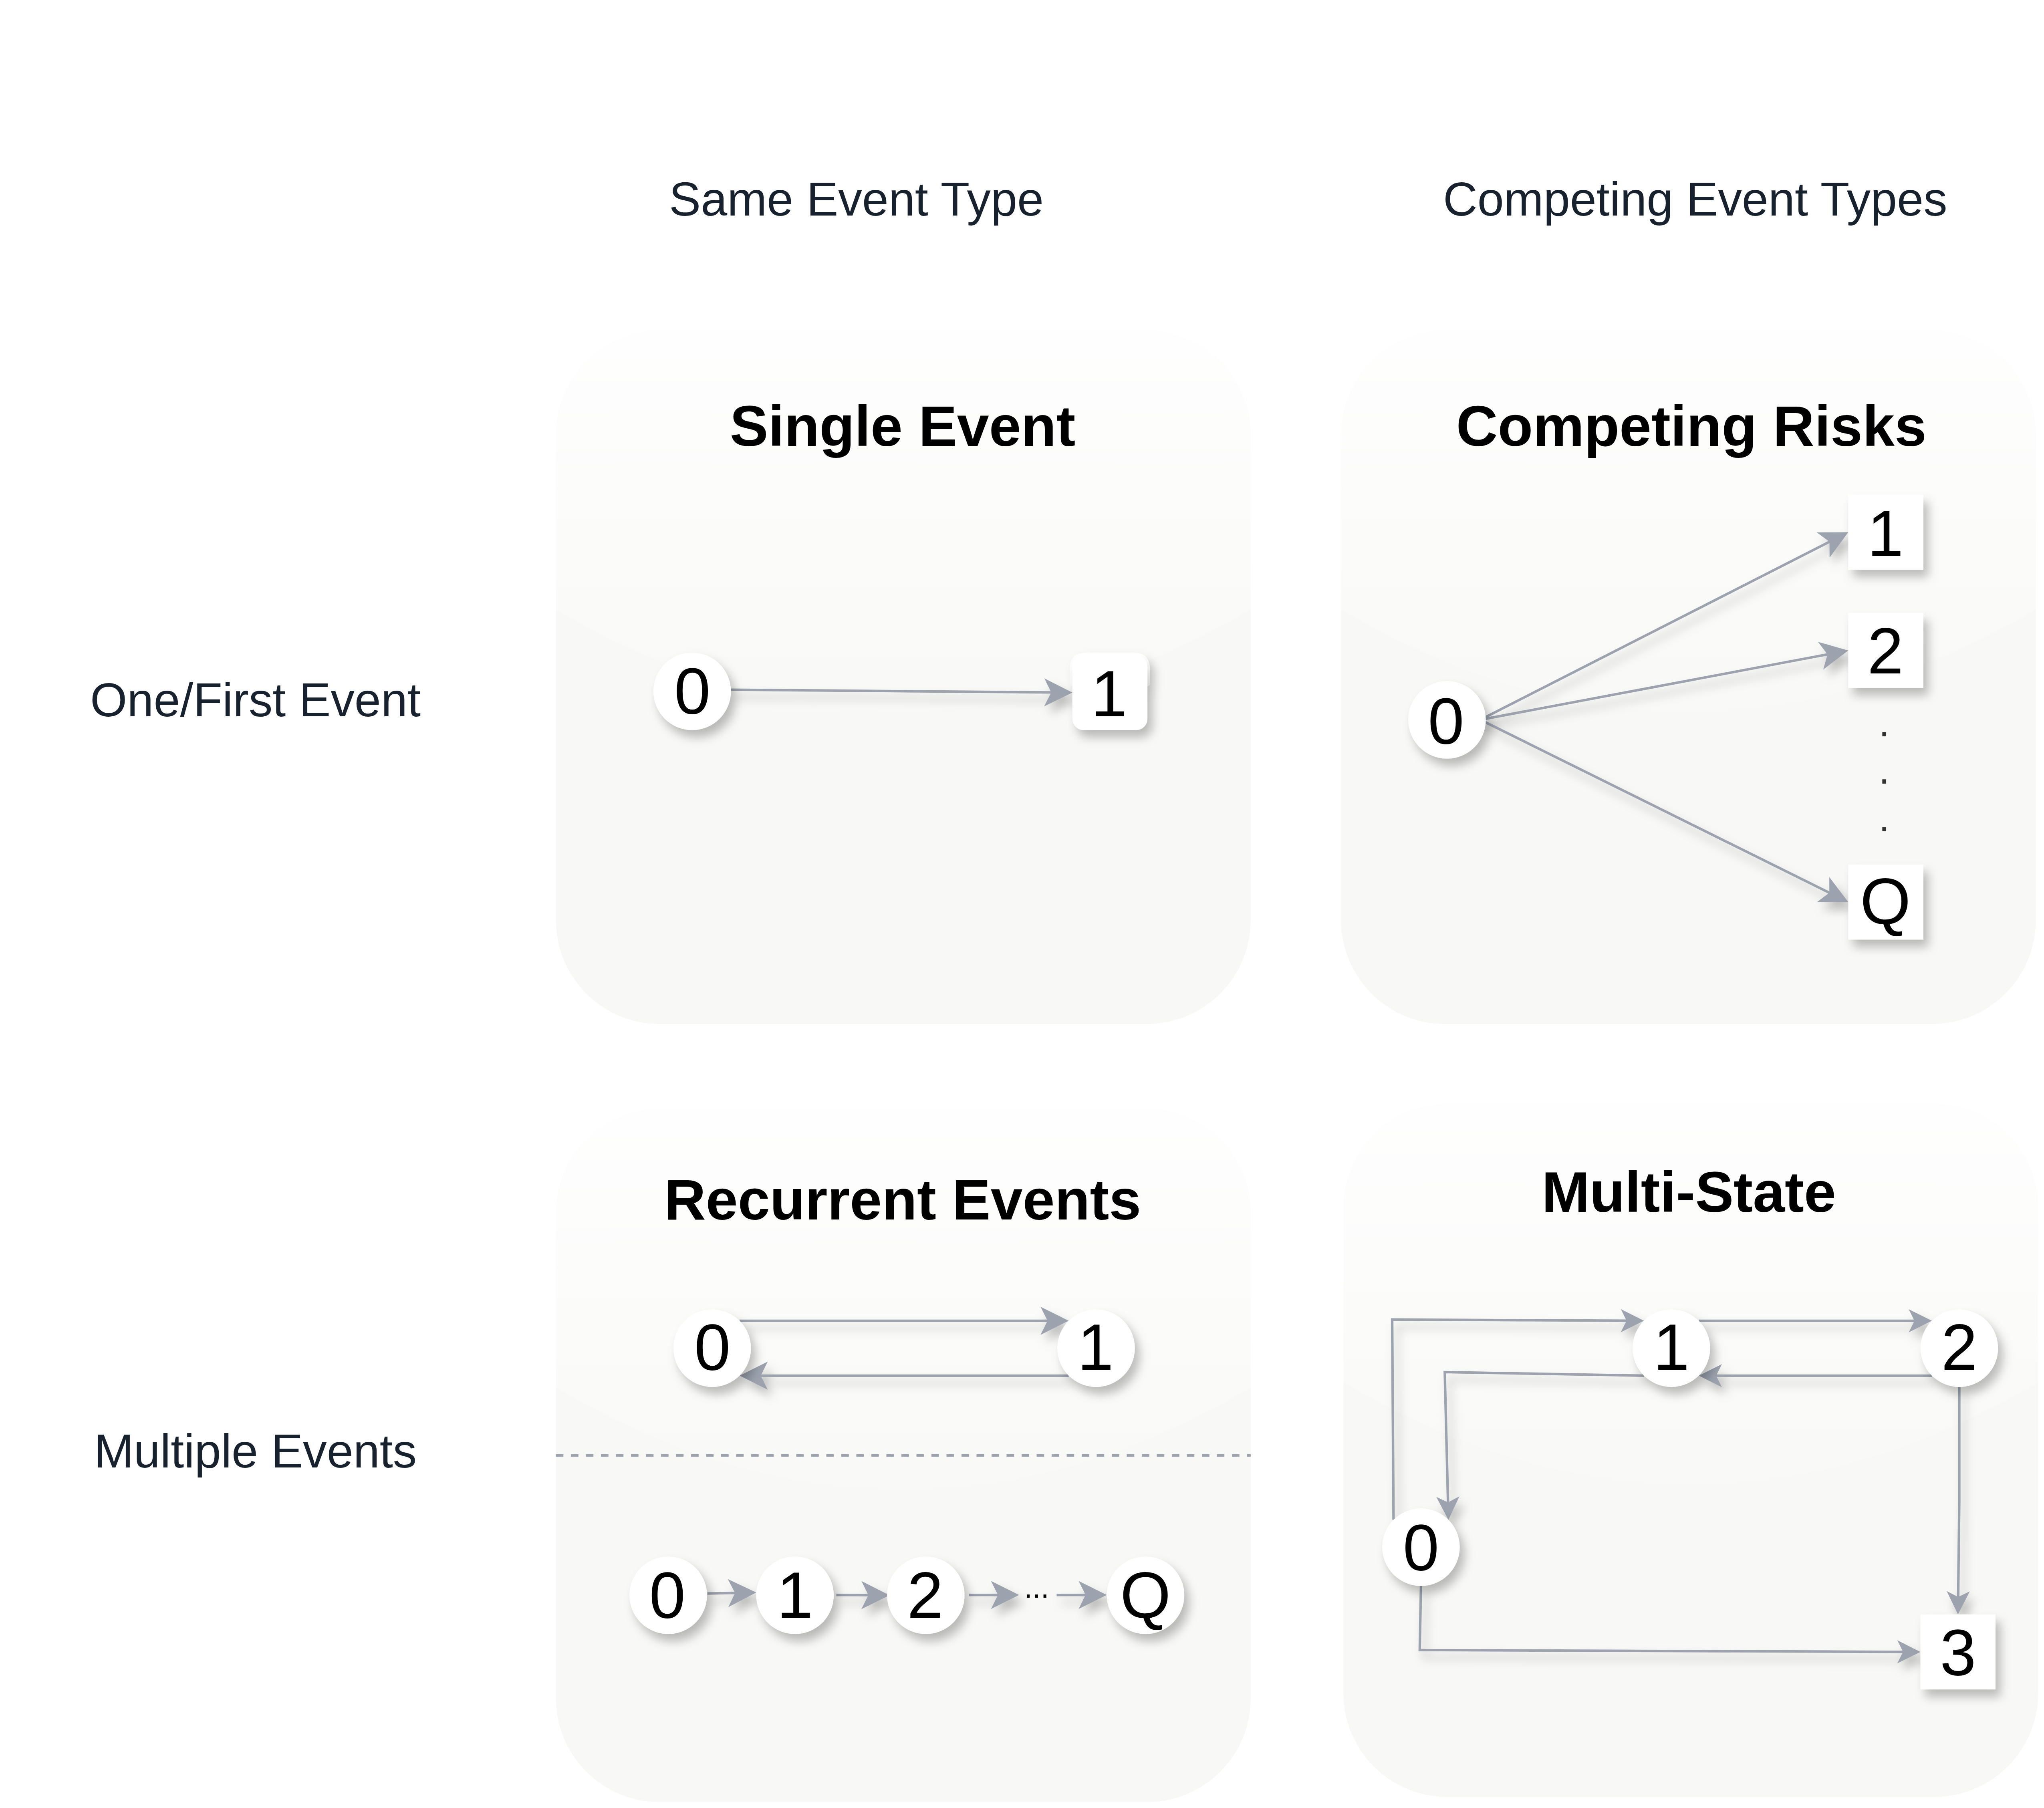
\includegraphics[width=0.7\linewidth,height=\textheight,keepaspectratio]{Figures/survival/fig-p1c5-eha-overview.png}

}

\caption{\label{fig-p1c5-eha-overview}Illustration of different types of
time-to-event processes. Transient states are displayed as circles,
terminal states are displayed as squares. Top-left: Standard
single-event setting with transition from initial state \(0\) to state
\(1\); Top-right: Competing risks setting with \(Q\) competing events.
The follow-up ends once one of the \(\{1,\ldots, Q\}\) events is
observed or the study ends; Bottom-left: Recurrent events setting with
multiple occurrences of the same event. Bottom-right: Multi-state
setting where subjects can transition between multiple transient states
with possible back-transitions or to terminal states.}

\end{figure}%

Note that the concepts discussed in Section~\ref{sec-types-of-censoring}
and Section~\ref{sec-truncation} are still relevant here, as, depending
on the specific process, any transition between two states could be
subject to different types of censoring and
truncation\index{censoring}\index{truncation}. Remaining in one of the
transient states until the end of follow-up constitutes
right-censoring\index{censoring!right}.
Left-truncation\index{truncation!left} is particularly important for the
multi-state setting as subjects enter the risk sets for each transition
at different time points, which must be individually accounted for
(Section~\ref{sec-non-param-lt}).

\section{A process point of view}\label{a-process-point-of-view}

In Chapter~\ref{sec-surv}, a subject is characterized by a single random
variable \(Y \in \mathbb{R}_{\geq 0}\), which represents the time until
the event of interest (defined in Section~\ref{sec-data-rc}). This
definition works well when exactly one event is possible or of interest.
However, when there are multiple possible events (for example, death by
heart disease versus cancer), recurrences (for example, hospital
re-admissions), or intermediate states (for example, healthy to ill to
recovered), a single scalar random variable no longer captures the
data-generating process. Instead, one tries to model which state the
subject is in at different moments in time.

A \emph{state} is a mutually exclusive classification of subjects at a
given time point\index{state process}. In the simplest single-event
setting, there are two states: ``no event yet'' (encoded by \(0\)) and
``event has occurred'' (encoded as \(1\)). In a competing-risks setting
with \(Q\) possible events, the states are \(\{0, 1, \ldots, Q\}\) with
\(0\) retaining the ``no event yet'' state and
\(q \in \{1, \ldots, Q\}\) indicating that event of type \(q\) has
occurred.

This is formalized as a stochastic process
\begin{equation}\phantomsection\label{eq-state-process}{
E(\tau) \in \{0,\ldots, Q\},\ \tau \geq 0,
}\end{equation} which records the state occupied at time \(\tau\). In
the single-event case (\(Q = 1\)), \(E(\tau)\) and \(Y\) provide the
same information. In particular,
\(\{Y \in [\tau, \tau + \,\mathrm{d}\tau) \mid Y \geq \tau\}\) and
\(\{E(\tau + \,\mathrm{d}\tau) = 1 \mid E(\tau-) = 0\}\) are
mathematically equivalent; the first expression represents the (only)
event of interest occurring in the next instant, the second is a jump
from state \(0\) to state \(1\) in the next instant. Thus their hazards
are equivalent,
\begin{equation}\phantomsection\label{eq-continuous-hazard-process}{
h(\tau)
  = \lim_{\,\mathrm{d}\tau\searrow 0}\frac{\Pr(Y \in [\tau, \tau + \,\mathrm{d}\tau) \mid Y \geq \tau)}{\,\mathrm{d}\tau}
  = \lim_{\,\mathrm{d}\tau\searrow 0}\frac{ \Pr\left(E(\tau + \,\mathrm{d}\tau)=1 \mid E(\tau-)=0\right)}{\,\mathrm{d}\tau},
}\end{equation} where \(\tau-\) indicates the time point immediately
before \(\tau\).

The process-valued formulation may seem over-engineered in the
single-event case but is less verbose when there are multiple states and
transitions, as will be seen in Section~\ref{sec-competing-risks} and
Section~\ref{sec-multi-state}. For a thorough stochastic-process
treatment of event history analysis, see Aalen, Borgan, and Gjessing
(2008).

\section{Competing risks}\label{sec-competing-risks}

Chapter~\ref{sec-surv} assumed a single event of interest, with all
reasons a subject might leave the observation window treated as
right-censoring. \emph{Competing risks}\index{competing risks} arise
when several mutually exclusive events can occur for the same subject.
Treating competing events as independent censoring can distort estimated
event probabilities; this is illustrated in
Section~\ref{sec-cens-vs-cr}. A canonical medical example is
cause-specific mortality, for example modeling if death was caused by
cancer or heart disease or another cause; another common example is
modeling death in an intensive care unit versus discharge. The defining
feature of the competing risks framework is that only one of the \(Q\)
events can occur on a subject at any given time. This section introduces
relevant notation (Section~\ref{sec-cr-notation}), the non-parametric
Aalen-Johansen estimator\index{Aalen-Johansen estimator}
(Section~\ref{sec-aalen-johansen}), and then a worked example.

Table~\ref{tbl-surv-data-siradm} shows an excerpt of the
\texttt{sir.adm} data (Allignol, Beyersmann, and Schumacher 2008) of
patients on an intensive care unit (ICU). Time under observation
(`time') could end in one of three outcomes (`status'): \(1\) ---
discharge alive; \(2\) --- death in the ICU; or \(0\) --- neither
discharge nor death at the end of follow-up, which constitutes
right-censoring at the end of study. The data were collected to
understand how pneumonia status at admission to the ICU affects
mortality.

In this study, follow-up stopped once patients were discharged. As
discharged patients are healthier than those who remain in the ICU,
assuming independence between the time until discharge and time until
death is unrealistic. Contrast this data to the \texttt{tumor} example
in Section~\ref{sec-surv-km}, in which patients were followed even after
hospital discharge. In that case, hospital discharge was not a competing
risk, even if a patient was lost to follow-up (thus right censored)
after discharge. Analysis of how these different assumptions
(independent censoring vs.~competing risks) affect the estimates is
discussed in Section~\ref{sec-aalen-johansen} and
Section~\ref{sec-cens-vs-cr}.

\begin{longtable}[]{@{}rrrl@{}}
\caption{Subset of the \texttt{sir.adm} dataset (Allignol, Beyersmann,
and Schumacher 2008). Each row represents one subject identified by
`id'. `time' is the time under observation, `status' indicates the
outcome observed (\(0\): censored at the end of the study, \(1\):
discharged from the ICU, \(2\): death in the ICU). `pneumonia' indicates
whether a subject had pneumonia at ICU
admission.}\label{tbl-surv-data-siradm}\tabularnewline
\toprule\noalign{}
id & time & status & pneumonia \\
\midrule\noalign{}
\endfirsthead
\toprule\noalign{}
id & time & status & pneumonia \\
\midrule\noalign{}
\endhead
\bottomrule\noalign{}
\endlastfoot
1 & 8 & 0 & no \\
2 & 8 & 0 & no \\
3 & 31 & 1 & yes \\
4 & 5 & 1 & no \\
5 & 9 & 2 & no \\
6 & 5 & 2 & no \\
\end{longtable}

\subsection{Notation and definitions}\label{sec-cr-notation}

In the competing risks setting, everyone starts in the initial state
\(0\) and can progress to one of the terminal states,

\[
q \in \{1,\ldots,Q\}.
\]

These terminal states\index{terminal states} are also often referred to
as \emph{competing events}, \emph{event types}, or \emph{causes}. State
\(q = 0\) is the initial state and a subject that remains in state \(0\)
until the end of follow-up is considered censored. The formulas in this
section characterize the process \(E(\tau) \in \{0,\ldots, Q\}\) in
terms of transition hazards and probabilities.

In extension of (\ref{eq-continuous-hazard-process}), the
\emph{cause-specific hazard} is defined as
\index{cause-specific hazard function},

\begin{equation}\phantomsection\label{eq-cause-specific-hazard}{
h_q(\tau) = \lim_{\,\mathrm{d}\tau\to 0} \frac{\Pr(E(\tau + \,\mathrm{d}\tau) = q\  \mid E(\tau-)=0)}{\,\mathrm{d}\tau}.
}\end{equation}

Analogous to the single-event case, the \emph{cause-specific cumulative
hazard}\index{cause-specific cumulative hazard function} is defined as,

\begin{equation}\phantomsection\label{eq-cause-specific-cumu-hazard}{
H_{q}(\tau) = \int_{0}^\tau h_q(u) \,\mathrm{d}u.
}\end{equation}

As competing events are mutually exclusive at any time \(\tau\), it is
possible to define the \emph{all-cause
hazard}\index{all-cause hazard function}, which is the hazard of any
event occurring as the sum of all cause-specific hazards,
\begin{equation}\phantomsection\label{eq-all-cause-hazard}{
h(\tau) = \sum_{q = 1}^Q h_q(\tau).
}\end{equation}

The \emph{all-cause cumulative
hazard}\index{all-cause cumulative hazard function} can then be
calculated either via the integral over the all-cause hazard
(\ref{eq-all-cause-hazard}) or as sum of cause-specific cumulative
hazards (\ref{eq-cause-specific-cumu-hazard}),

\begin{equation}\phantomsection\label{eq-all-cause-cumu-hazard}{
H(\tau) 
 = \sum_{q=1}^Q H_{q}(\tau) = \sum_{q=1}^{Q}\int_{0}^\tau h_{q}(u) \,\mathrm{d}u
 =\int_{0}^\tau \sum_{q=1}^{Q} h_{q}(u) \,\mathrm{d}u= \int_{0}^\tau h(u) \,\mathrm{d}u.
}\end{equation}

The \emph{all-cause survival
probability}\index{all-cause survival function} gives the probability
that \emph{none} of the events occurred before \(\tau\). This is usually
not estimated directly but calculated from the cause-specific hazards
via (\ref{eq-all-cause-cumu-hazard}),

\begin{equation}\phantomsection\label{eq-all-cause-surv-prob}{
S(\tau) = \Pr(Y > \tau) = \Pr(E(\tau) = 0) = \exp(-H(\tau)).
}\end{equation}

Finally, the \emph{cumulative incidence function}
(CIF)\index{cumulative incidence function} is the probability of
experiencing an event \(q\) before time \(\tau\),

\begin{equation}\phantomsection\label{eq-cif}{
F_q(\tau) = \Pr(E(\tau) = q)  = \int_{0}^\tau f_q(u) \mathrm{d}u = \int_{0}^\tau S(u-)h_q(u)\ \,\mathrm{d}u,
}\end{equation}

where \(S(u-)\) is the probability of surviving (not experiencing any of
the competing events) until the time point shortly before \(u\); and
\(f_q(u)\,\mathrm{d}u= S(u-)h_q(u)\,\mathrm{d}u\) is the probability of
experiencing event \(q\) in a small interval around \(u\) (which follows
analogously to the relationship between density and hazard functions in
(\ref{eq-continuous-hazard})). All the terms in (\ref{eq-cif}) can be
calculated from the cause-specific hazards
(\ref{eq-cause-specific-hazard}) and estimation of the CIF often takes
this `cause-specific hazards' approach.

The notation \(S(u-)\) is used rather than \(S(u)\) to make explicit the
modeling of the probability to survive until the time point immediately
before \(u\). This makes limited difference in continuous time where
\(\Pr(T > t) = \Pr(T\geq t)\), but may be important in (discrete)
approximations (discussed in Section~\ref{sec-aalen-johansen}).

\(F_q(\tau)\) can be interpreted as the proportion of subjects who
experienced event of type \(q\) before time \(\tau\). Because the events
are mutually exclusive, it holds that \[
S(\tau) + \sum_{q=1}^Q F_q(\tau) =  S(\tau) + F(\tau)= 1
\] where \(F(\tau)\) is the probability that any event occurs before
\(\tau\), and \(S(\tau)\) is the all-cause survival probability
(\ref{eq-all-cause-surv-prob}).

\subsection{Non-parametric estimators}\label{sec-aalen-johansen}

Estimating the CIF (\ref{eq-cif}) for cause \(q\) requires estimates of
two components: the all-cause survival function \(S(t)\) and the
cause-specific hazard \(h_q(t)\), both of which can be estimated
non-parametrically through direct analogues of the single-event
constructions in Section~\ref{sec-surv-estimation-non-param}.

Recall from Section~\ref{sec-data-rc} the unique ordered event times
\(t_{(k)},\, k=1,\ldots,m\), the risk set \(\mathcal{R}_{t_{(k)}}\), and
the number at risk \(n_{t_{(k)}}\). Assume the follow-up is partitioned
into \(m\) disjoint intervals \((t_{(k-1)}, t_{(k)}],\, k=1,\ldots,m\),
such that
\(Y \in (t_{(k-1)}, t_{(k)}] \Leftrightarrow \tilde{Y}=t_{(k)}\), with
\(\tilde{Y}\) the discrete time random variable defined in
Section~\ref{sec-distributions-discrete}.

Let \(d_{q,t_{(k)}}\) be the number of events of type \(q\) observed at
\(t_{(k)}\). Then the \emph{cause-specific} discrete hazard is the
analogue of the discrete hazard estimator (\ref{eq-disc-haz-non-param}),
with the numerator restricted to events of type \(q\),
\begin{equation}\phantomsection\label{eq-cs-discrete-hazard}{
h^d_{q}(t_{(k)}) := \frac{d_{q,t_{(k)}}}{n_{t_{(k)}}},\ q \in \{1, \ldots, Q\}.
}\end{equation}

The all-cause survival probability\index{all-cause survival function}
(\ref{eq-all-cause-surv-prob}) can be estimated with the Kaplan-Meier
estimator\index{Kaplan-Meier estimator} (\ref{eq-km}). Substituting this
estimate and (\ref{eq-cs-discrete-hazard}) into (\ref{eq-cif}), yields
the Aalen-Johansen (AJ) estimator\index{Aalen-Johansen estimator} (Aalen
and Johansen 1978) for the CIF of cause \(q\),

\begin{equation}\phantomsection\label{eq-aalen-johansen}{
F_{AJ,q}(\tau) = \sum_{k:t_{(k)}\leq \tau} S_{KM}(t_{(k-1)})h^d_q(t_{(k)})=  \sum_{k:t_{(k)}\leq \tau} S_{KM}(t_{(k-1)})\frac{d_{q,t_{(k)}}}{n_{t_{(k)}}}.
}\end{equation}

\subsection{Application to mortality of ICU
patients}\label{application-to-mortality-of-icu-patients}

For illustration of the AJ estimator and the interpretation of the
CIFs\index{cumulative incidence function} consider the analysis based on
the data from Table~\ref{tbl-surv-data-siradm}. Recall from the start of
this section, the objective was to estimate mortality (state \(2\))
given pneumonia status at admission, with discharge from ICU as a
competing risk (state \(1\)). While the AJ estimator cannot naturally
incorporate feature information, it can be applied to subgroups of the
data, here based on the pneumonia status
\(x_{\text{pneu}} \in \{0,1\}\). Note that this will yield different
sets of unique event times in each group, thus the AJ can have jumps at
different time points for the two groups.

Figure~\ref{fig-p1c5-cif-sir} shows the AJ estimates of the CIFs for the
two competing events stratified by pneumonia status. To give a few
examples, approximately 75\% of patients with pneumonia have been
discharged by \(\tau = 120\) days:

\[
\hat{F}_{1}(120 \mid x_{\text{pneu}}=1) = \widehat{\Pr}(E(120) = 1 \mid x_{\text{pneu}}=1)\approx 0.75,
\]

while approximately 25\% died in the ICU:

\[
\hat{F}_2(120 \mid x_{\text{pneu}}=1) = \widehat{\Pr}(E(120) = 2 \mid x_{\text{pneu}}=1)\approx 0.25.
\]

For patients without pneumonia,

\[
\hat{F}_{1}(120 \mid x_{\text{pneu}}=0) \approx 0.91,
\]

and

\[
\hat{F}_{2}(120 \mid x_{\text{pneu}}=0) \approx 0.09.
\]

\begin{figure}

\centering{

\pandocbounded{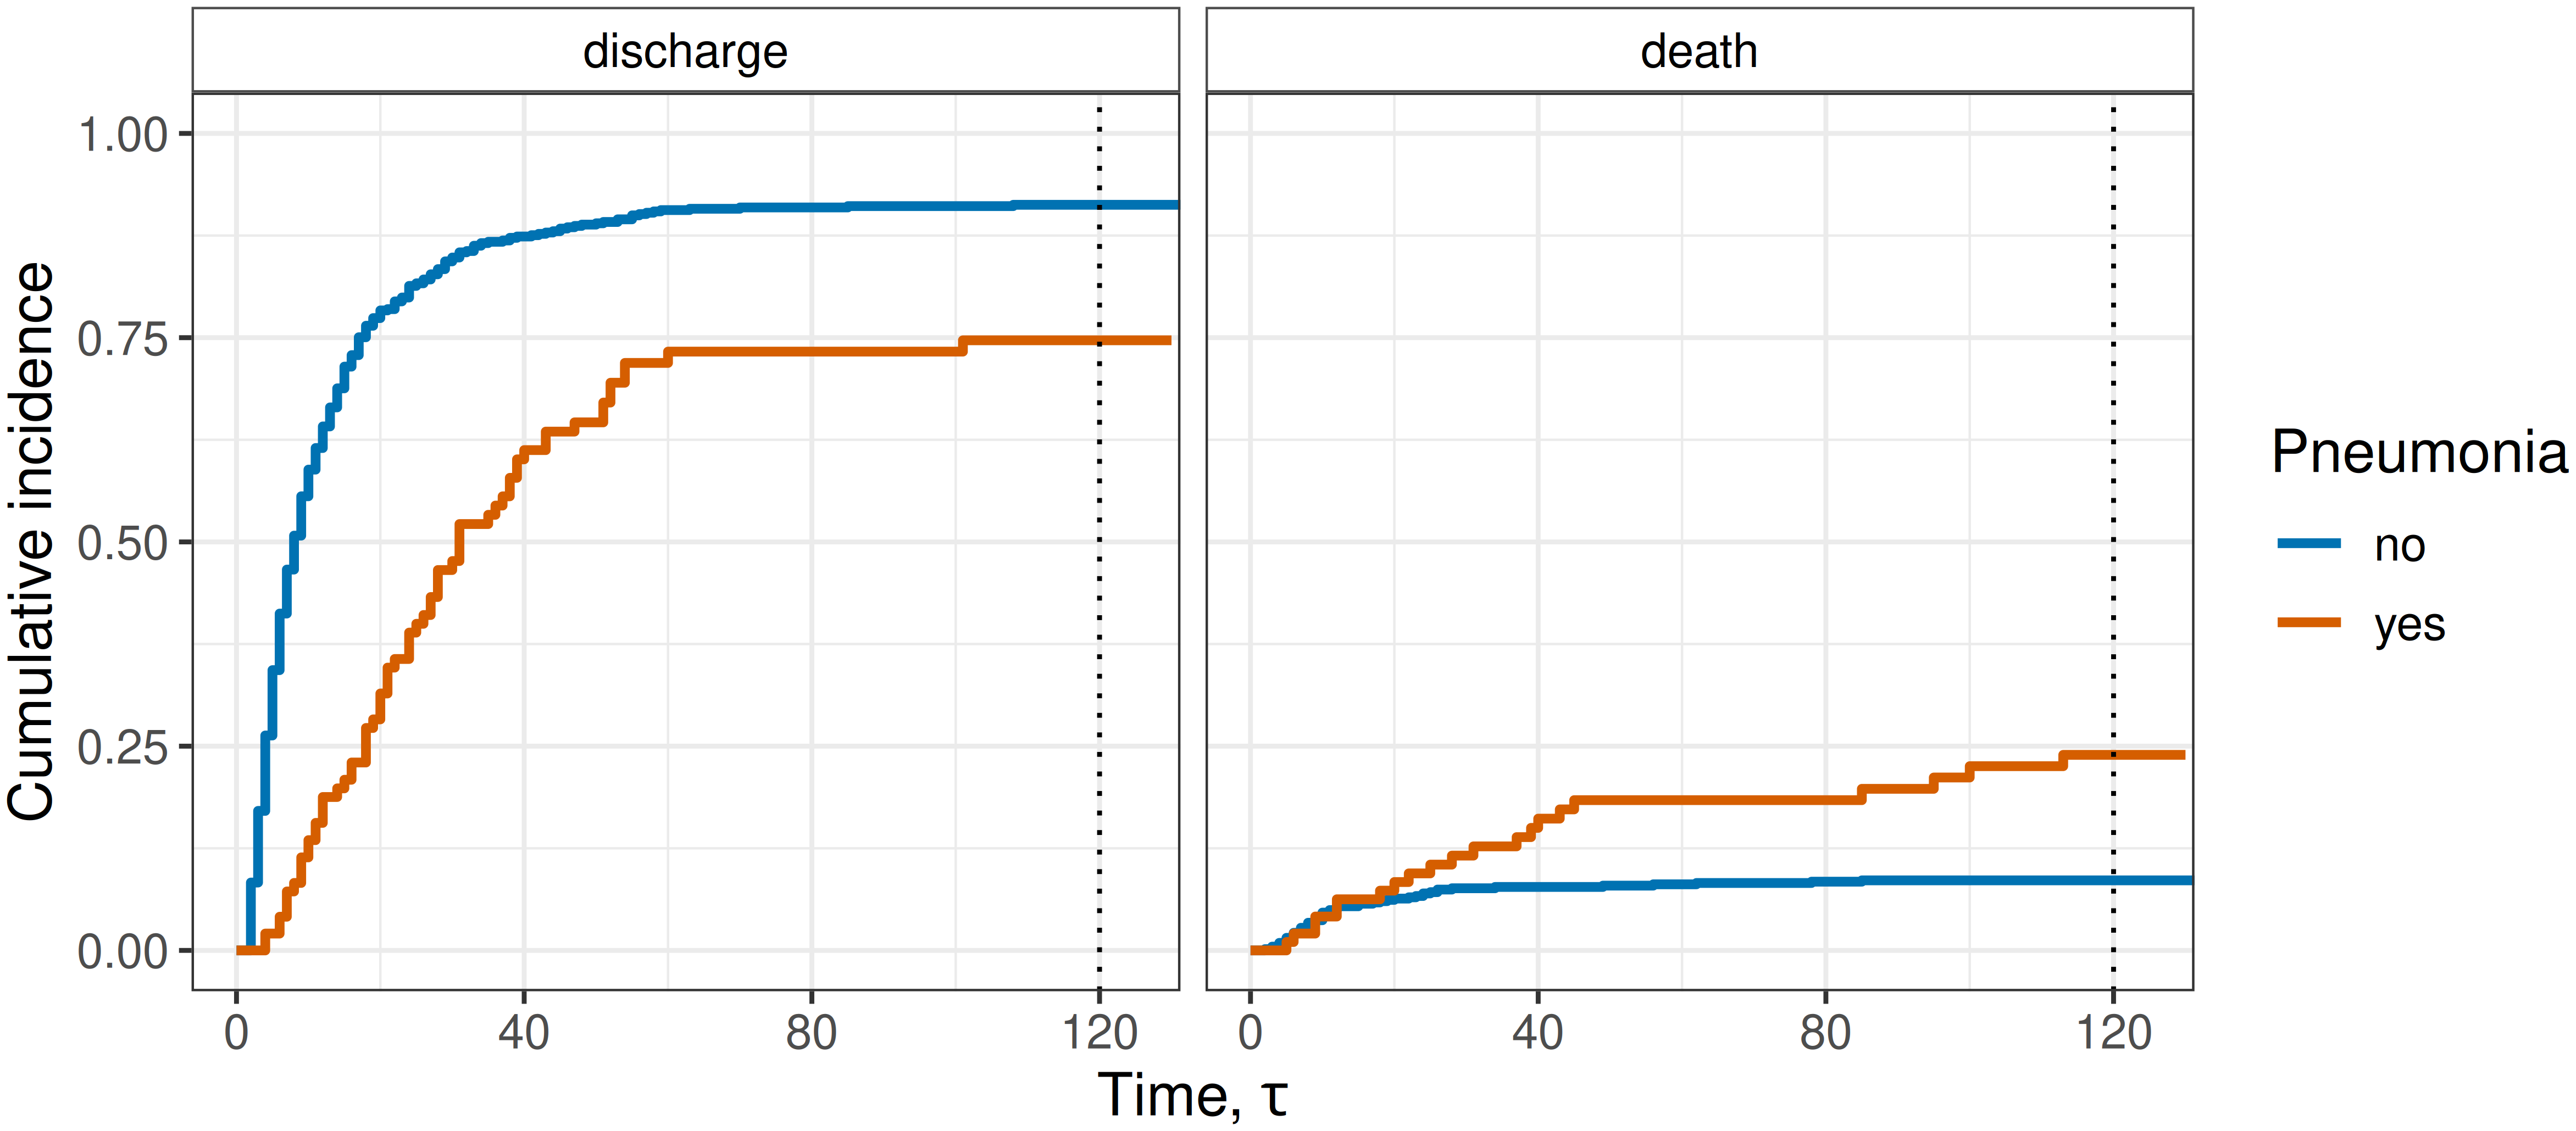
\includegraphics[keepaspectratio]{Figures/survival/fig-p1c5-cif-sir.png}}

}

\caption{\label{fig-p1c5-cif-sir}Aalen-Johansen estimator for the
\texttt{sir.adm} data (Allignol, Beyersmann, and Schumacher 2008),
stratified by pneumonia status at admission to the ICU. Left panel:
Proportion of subjects discharged alive from the ICU. Right panel:
Proportion of subjects who died in the ICU.}

\end{figure}%

\subsection{Independent censoring vs.~competing
risks}\label{sec-cens-vs-cr}

When estimating the cause-specific discrete hazard
(\ref{eq-cs-discrete-hazard}) for cause \(q\), all events of type
\(\tilde{q} \neq q\) are treated as if they were
right-censored\index{censoring!right}. However, these competing events
are subsequently combined when calculating the CIF (\ref{eq-cif}), for
example through the AJ estimator (\ref{eq-aalen-johansen}), in which the
all-cause survival probability (\ref{eq-all-cause-surv-prob}) depends on
all the cause-specific hazards.

The competing risks approach was just illustrated in the analysis of the
\texttt{sir.adm} data. Consider instead if discharge were treated as an
independent right-censoring event and not as a competing risk. In that
case, the event of interest (death) could be modeled using the methods
in Chapter~\ref{sec-surv}, for example using the Nelson-Aalen
estimator\index{Nelson-Aalen estimator} (\ref{eq-surv-na}). The
estimated probability of death before some time point \(\tau\) could
then be obtained via \(\hat{F}(\tau) = 1 - \hat{S}_{NA}(\tau)\).

Figure~\ref{fig-p1c5-cens-vs-cr} shows the estimates obtained under the
two assumptions. Solid lines indicate the probabilities under the
competing risks assumption (identical to the right-hand side of
Figure~\ref{fig-p1c5-cif-sir}). Dashed lines are obtained under the
independent right-censoring assumption. Clearly, the probabilities of
dying by time \(\tau=120\) are much larger when independent censoring is
assumed; for example around 75\% in the pneumonia group under the
right-censoring assumption, compared to around 25\% when discharge is
correctly modeled as a competing risk. This example emphasizes the
importance of assessing which modeling framework is appropriate for a
given analysis, as the resulting estimates may differ substantially.

\begin{figure}

\centering{

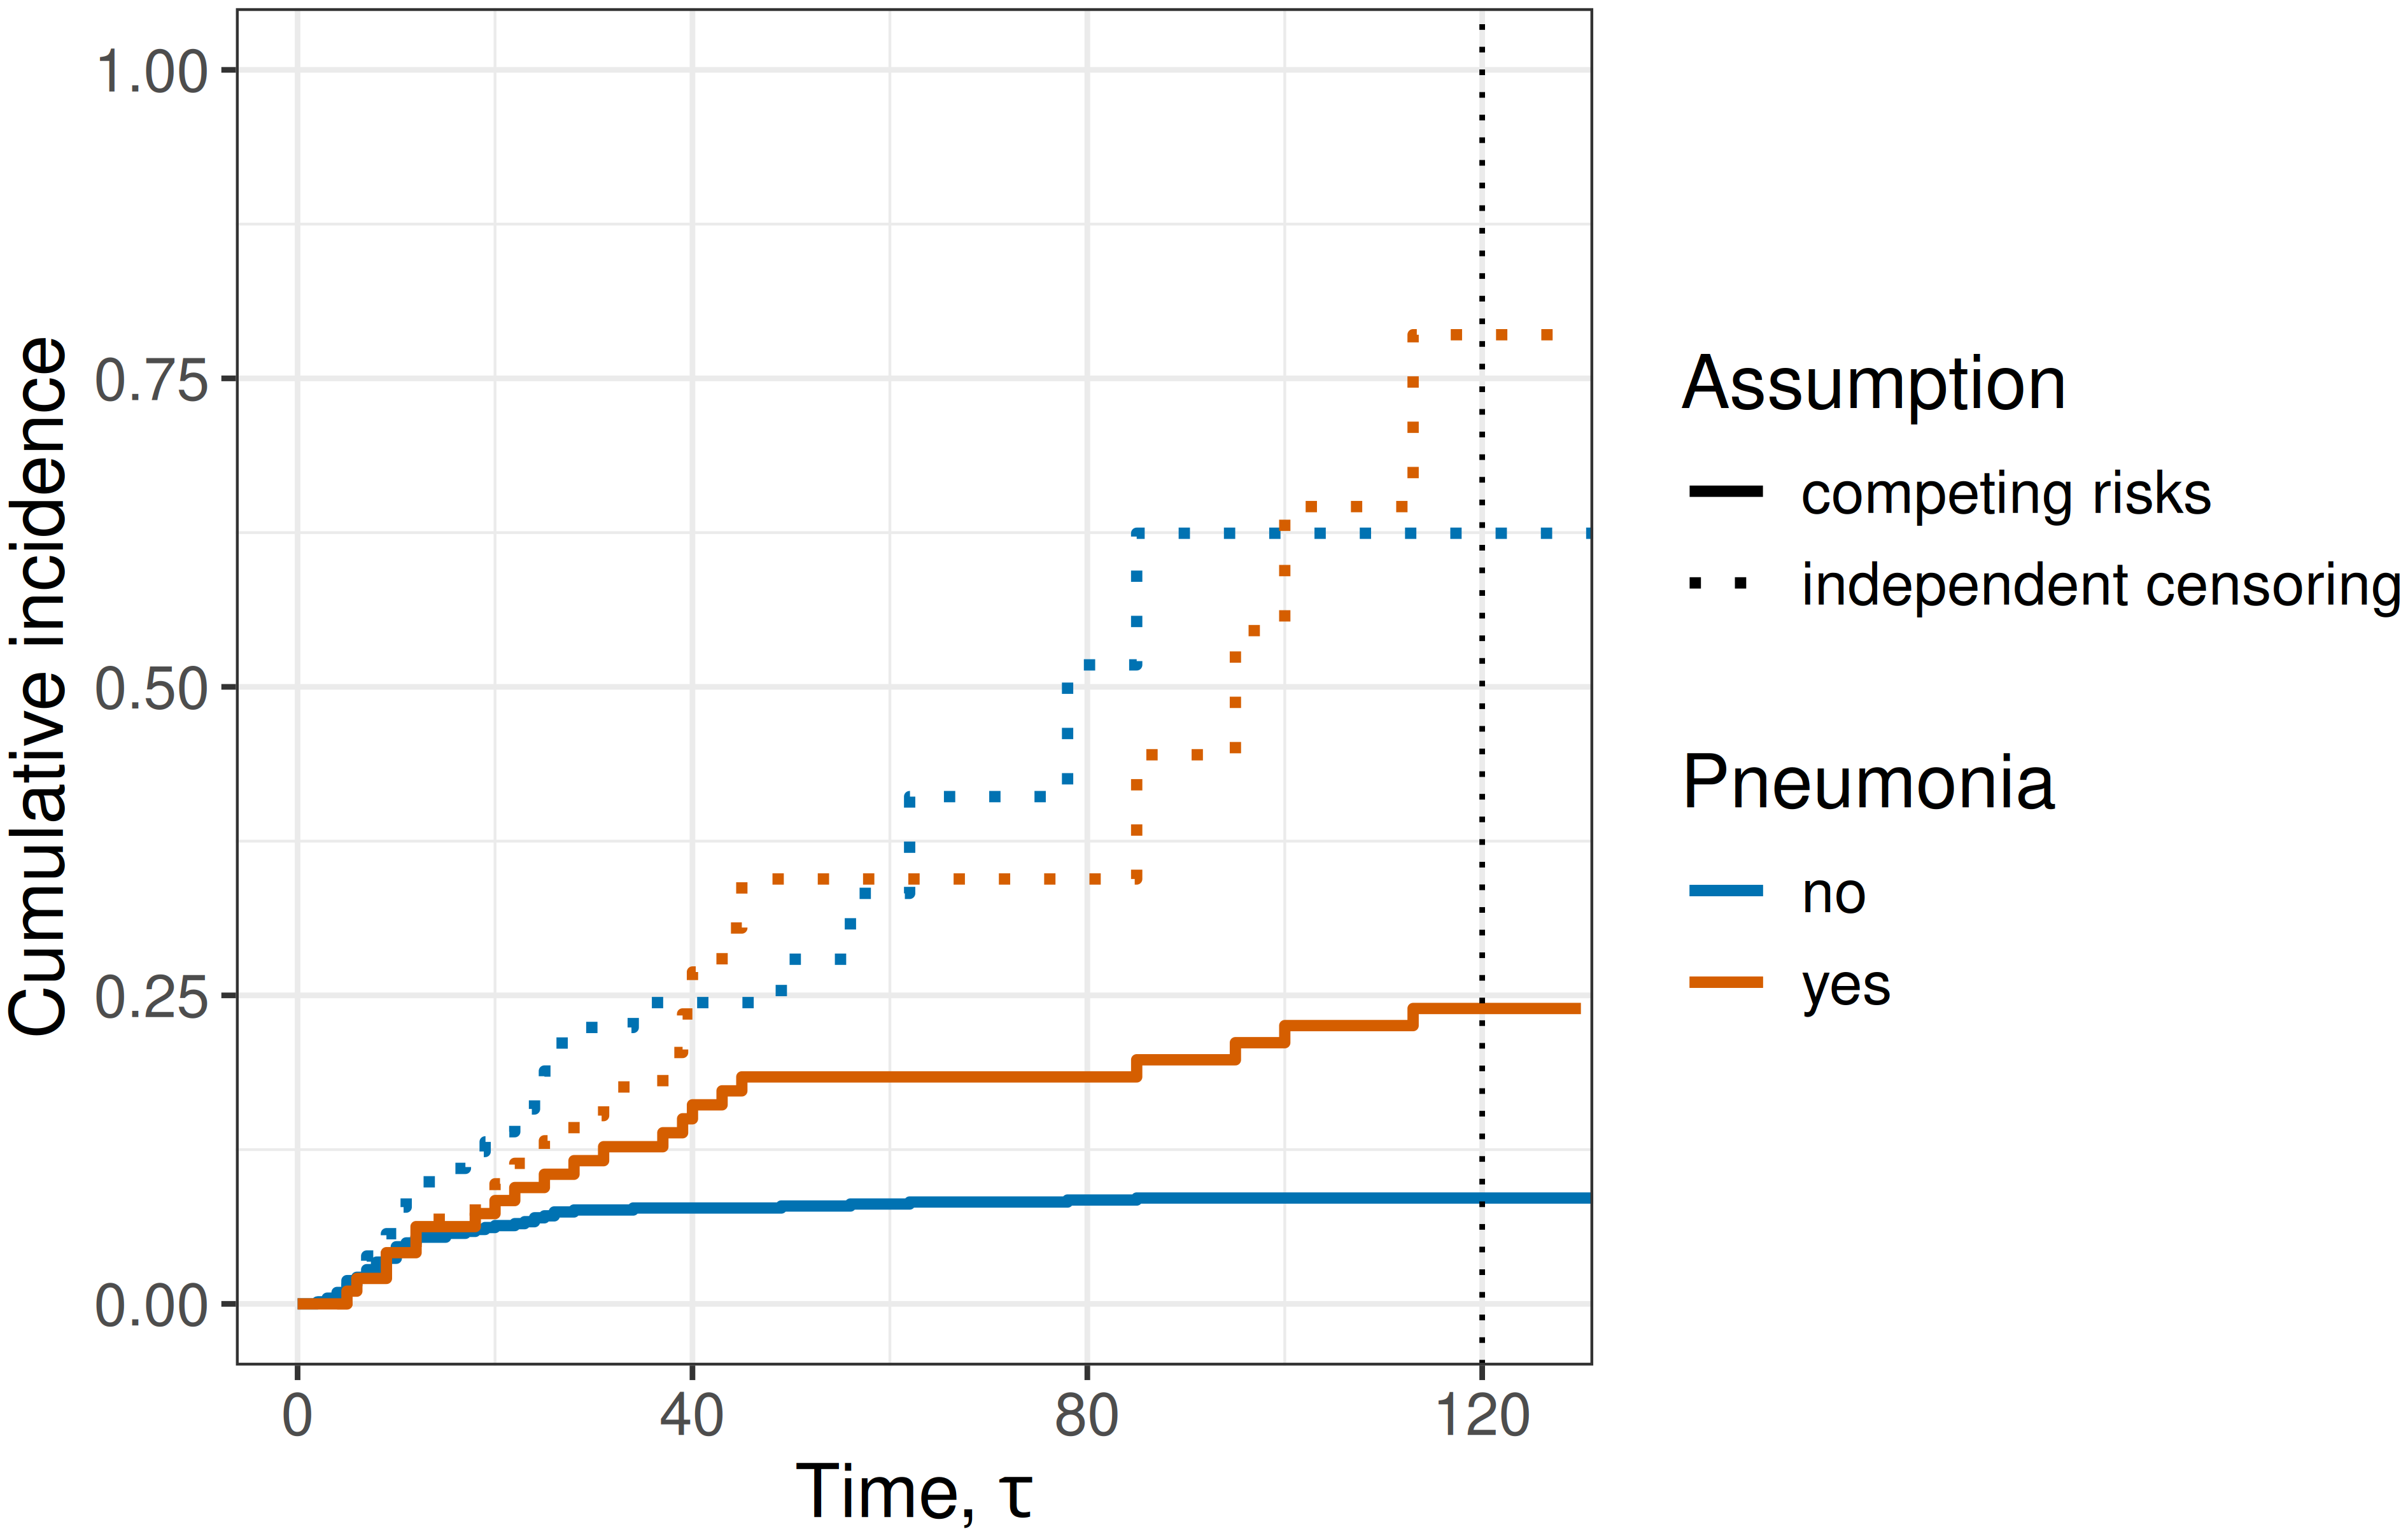
\includegraphics[width=0.7\linewidth,height=\textheight,keepaspectratio]{Figures/survival/fig-p1c5-cens-vs-cr.png}

}

\caption{\label{fig-p1c5-cens-vs-cr}Estimation of the probability of
dying in the ICU conditional on pneumonia status at admission. Dashed
lines give the probabilities under assumption of right-censoring. Solid
lines give the probabilities when taking into account discharge as
competing risk.}

\end{figure}%

\section{Multi-state models}\label{sec-multi-state}

The multi-state process\index{multi-state models} can be considered the
most general type of time-to-event process, as others (single-event,
competing risks\index{competing risks}, recurrent
events\index{recurrent events}) can be viewed as special cases.
Multi-state modeling allows realistic depiction of complex processes
where subjects can start in different states and transition back and
forth between them\index{state process}.

For illustration, consider the \texttt{prothr} dataset (de Wreede,
Fiocco, and Putter 2011) of liver cirrhosis patients from a randomized
clinical trial with possible transitions depicted in
Figure~\ref{fig-p1c5-multi-state-prothr-states}. Patients may have
normal (state \(0\)) or abnormal (state \(1\)) levels of prothrombin (a
protein important for blood clotting, produced by the liver) at the
beginning of the trial. Some patients were treated with prednisone
(which suppresses immune response and reduces inflammation) and others
received a placebo. Death (state \(2\)) constitutes the terminal state.
The purpose of the trial was to investigate if treatment (prednisone)
slows down or reverses disease progression (transitions
\(0 \rightarrow 1\) and \(1 \rightarrow 0\)) and/or reduces mortality
(transitions \(0 \rightarrow 2\) and \(1 \rightarrow 2\)).

\begin{figure}

\centering{

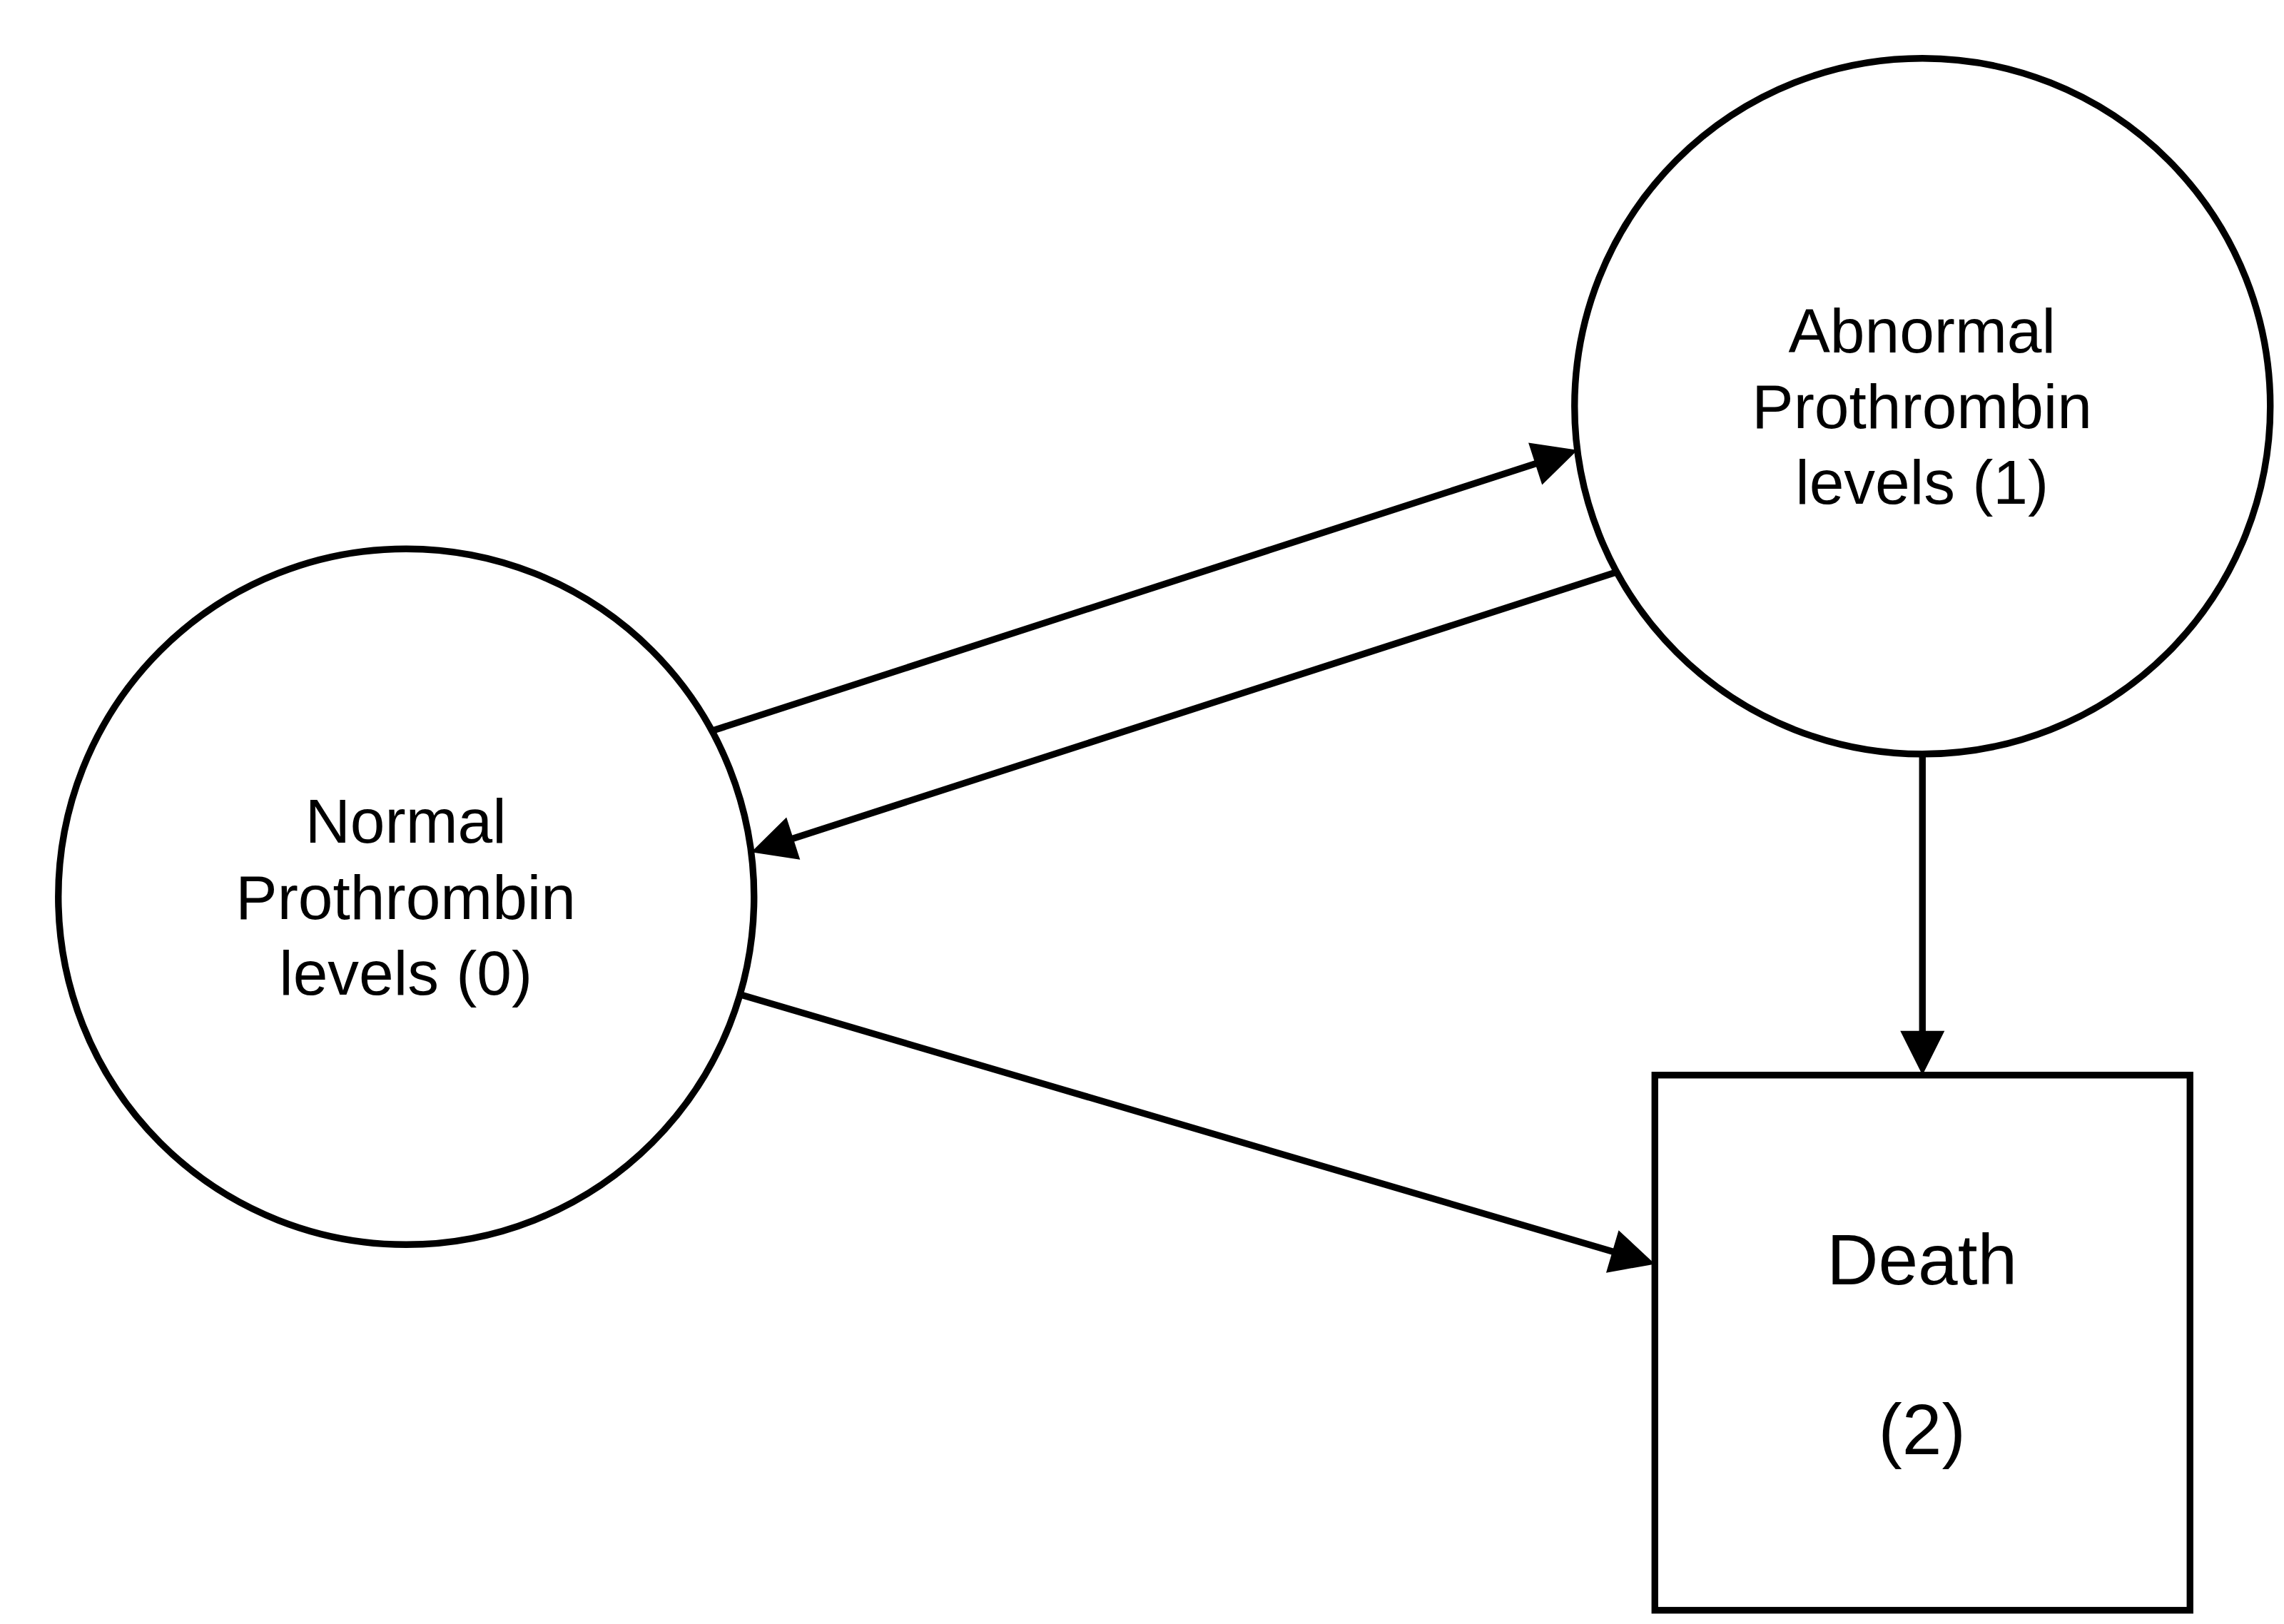
\includegraphics[width=0.6\linewidth,height=\textheight,keepaspectratio]{Figures/survival/fig-p1c5-multi-state-prothr-states.png}

}

\caption{\label{fig-p1c5-multi-state-prothr-states}Transition graph for
the liver cirrhosis patients.}

\end{figure}%

Strictly speaking, prothrombin level is only assessed at scheduled
follow-up visits, so the transitions between state \(0\) (normal) and
state \(1\) (abnormal) are interval-censored\index{censoring!interval}
(Section~\ref{sec-types-of-censoring-left-interval}): at visit \(k\) the
new status is observed, but not the exact time at which the change
occurred between visits \(k-1\) and \(k\). The analyses that follow
ignore this interval structure and treat the transition times as exactly
observed, which is a common simplification for this example. Accounting
for the interval-censoring would require similar non-parametric maximum
likelihood estimator\index{non-parametric maximum likelihood estimator}
methods to those described in
Section~\ref{sec-surv-estimation-non-param}.

Table~\ref{tbl-ms-data-prothr} shows a subset of the data and contains,
for each subject (`id'), one row per transition for which the subject
was at risk. In this example, this includes transitions that were
possible, but did not happen (counterfactual transitions). The columns
`from' and `to' indicate the initial state and the possible end state of
each transition, which the `transition' column also shows compactly as
\(\ell \rightarrow q\). `tstart' indicates the time at which the subject
entered the `from' state and thereby became at risk for the transition
listed in that row, and `tstop' the time at which the subject left the
`from' state, either by making a transition or by being censored. The
variable `status' indicates whether the transition was actually made
(`status=1') or not (`status=0'). The status variable is required here
as all possible transitions are listed (including counterfactuals), so
an indicator is required to identify which transitions actually
occurred. If `status=0' for all possible transitions, the subject is
censored for further transitions. Finally, `treatment' indicates whether
a patient was assigned the treatment or placebo group.

Subject `id=1' already had abnormal prothrombin levels at the beginning
of the trial, thus started in state \(1\) with possible transitions
\(1\rightarrow 0\) and \(1 \rightarrow 2\). In this case, the patient
died and transition \(1\rightarrow 2\) was realized after 151 days,
while the transition \(1 \rightarrow 0\) is a `counterfactual'
transition that could have happened in the time-span between `tstart=0'
and `tstop=151', but did not actually occur in reality. Patient `id=8'
also started in state \(1\), but made a back transition to normal
prothrombin levels after 211 days at which time they entered the risk
set for transitions \(0\rightarrow 1\) and \(0\rightarrow 2\). Neither
of the transitions occurred, as `status=0' for both transitions, which
means the subject remained in state \(0\) (right-censored) until the end
of their follow-up at 2,770 days. Finally, subject `id=46' started in
state 0 (normal levels), transitioned to state 1 (abnormal levels) after
415 days and then died (transition \(1\rightarrow 2\)) two days later.

This example illustrates the importance of left-truncation
(Section~\ref{sec-truncation}) in multi-state processes. For example,
subjects `id=1' and `id=8' are at risk for the transitions
\(1 \rightarrow 0\) and \(1 \rightarrow 2\) from the beginning of the
trial (`tstart = 0'). In contrast, subject `id=46' starts in state 0 and
only enters state \(1\), thus the risk set for the transitions
\(1\rightarrow 0\) and \(1\rightarrow 2\), after 415 days (`tstart =
415'). The fact that subjects enter the risk sets for different
transitions at different time points constitutes left-truncation and
should be taken into account accordingly
(Section~\ref{sec-ms-aalen-johansen}).

\begin{longtable}[]{@{}rrrcrrrl@{}}
\caption{Subset of the \texttt{prothr} dataset (de Wreede, Fiocco, and
Putter 2011). Each row is a transition for which the subject (`id') was
at risk: `from'/`to' (also shown as `transition',
\(\ell \rightarrow q\)) are the start and possible end states;
`tstart'/`tstop' are the times of entering and leaving the `from' state;
`status' is \(1\) if the transition occurred and \(0\) otherwise; and
`treatment' is the trial arm.}\label{tbl-ms-data-prothr}\tabularnewline
\toprule\noalign{}
id & from & to & transition & tstart & tstop & status & treatment \\
\midrule\noalign{}
\endfirsthead
\toprule\noalign{}
id & from & to & transition & tstart & tstop & status & treatment \\
\midrule\noalign{}
\endhead
\bottomrule\noalign{}
\endlastfoot
1 & 1 & 0 & \(1 \rightarrow 0\) & 0 & 151 & 0 & Placebo \\
1 & 1 & 2 & \(1 \rightarrow 2\) & 0 & 151 & 1 & Placebo \\
8 & 1 & 0 & \(1 \rightarrow 0\) & 0 & 211 & 1 & Prednisone \\
8 & 1 & 2 & \(1 \rightarrow 2\) & 0 & 211 & 0 & Prednisone \\
8 & 0 & 1 & \(0 \rightarrow 1\) & 211 & 2770 & 0 & Prednisone \\
8 & 0 & 2 & \(0 \rightarrow 2\) & 211 & 2770 & 0 & Prednisone \\
46 & 0 & 1 & \(0 \rightarrow 1\) & 0 & 415 & 1 & Prednisone \\
46 & 0 & 2 & \(0 \rightarrow 2\) & 0 & 415 & 0 & Prednisone \\
46 & 1 & 0 & \(1 \rightarrow 0\) & 415 & 417 & 0 & Prednisone \\
46 & 1 & 2 & \(1 \rightarrow 2\) & 415 & 417 & 1 & Prednisone \\
\end{longtable}

\subsection{Notation and definitions}\label{notation-and-definitions}

In the competing risks setting, the data generating process was
characterized by cause-specific transition hazards \(h_q(\tau)\)
(\ref{eq-cause-specific-hazard}). Implicitly, these are transitions from
starting state \(0\) to end state \(q\); however, since everyone starts
in state \(0\), more complex notation is not required. In the
multi-state setting, with multiple different states and more complex
transitions, more sophisticated notation is necessary. Transitions
between different states are characterized by transition hazards,
denoted by \(h_{\ell\rightarrow q}(\tau)\) or more simply
\(h_{\ell q}(\tau)\), where \(\ell\) is the starting state and \(q\) the
end state.

Let \(E(\tau)\in \{0,\ldots,Q\}\) be the state of the process at time
\(\tau\) as in (\ref{eq-state-process}). Then, the \emph{transition
hazard}\index{transition hazard function} can be defined as,
\begin{equation}\phantomsection\label{eq-ms-transition-hazards}{
h_{\ell q}(\tau) = \lim_{\,\mathrm{d}\tau\to 0} \frac{\Pr(E(\tau + \,\mathrm{d}\tau)=q \mid E(\tau-) = \ell)}{\,\mathrm{d}\tau}.
}\end{equation}

Transition hazards (\ref{eq-ms-transition-hazards}) indicate the
instantaneous risk to enter state \(q\) at time \(\tau\) given
occupation of state \(\ell\) at \(\tau-\), which is the instant before
\(\tau\).

By definition, a transition is a move \emph{out} of the current state
and therefore \(\ell \neq q\) when describing the transition hazard
\(h_{\ell q}(\tau)\). Furthermore, not every pair \((\ell, q)\)
corresponds to a realizable transition: the state diagram of the
specific process determines which transitions are possible a priori (for
example, Figure~\ref{fig-p1c5-multi-state-prothr-states}), and the
hazards of impossible transitions are equal to zero.

Analogous to the competing risks setting, one can define the
\emph{transition cumulative
hazard}\index{transition cumulative hazard function},

\begin{equation}\phantomsection\label{eq-ms-cumu-hazard}{
H_{\ell q}(\tau) = \int_{0}^{\tau}h_{\ell q}(u) \,\mathrm{d}u.
}\end{equation}

In the multi-state setting, two further quantities are often of
interest. Firstly, the \emph{transition
probabilities}\index{transition probability}

\[
P_{\ell q}(\zeta, \tau):= \Pr(E(\tau) = q \mid E(\zeta) = \ell),
\]

that is, the conditional probability to be in state \(q\) at \(\tau\)
given occupation of state \(\ell\) at \(\zeta < \tau\) (fully introduced
in Section~\ref{sec-ms-transition-probs}).

Secondly, the (marginal) \emph{state-occupation
probability}\index{state-occupation probability},

\begin{equation}\phantomsection\label{eq-ms-state-prob}{
\Pr(E(\tau) = q),
}\end{equation}

which is the probability to occupy a certain state \(q\) at time
\(\tau\) (described in detail in Section~\ref{sec-ms-state-occupation}).

Throughout the remainder of Section~\ref{sec-multi-state}, it is assumed
that the multi-state process is \emph{Markov}\index{Markov}, meaning
that the transition hazard at time \(\tau\) depends only on the current
state \(E(\tau-)\) and not on the full state history
\(\{E(u) : u < \tau\}\). Under this assumption, conditioning on the
current state alone (as in (\ref{eq-ms-transition-hazards})) is
sufficient to characterize the local dynamics, and the transition
probability \(P_{\ell q}(\zeta,\tau)\) is fully determined by the
transition cumulative hazards between \(\zeta\) and \(\tau\). The
non-parametric Aalen-Johansen estimator\index{Aalen-Johansen estimator}
(\ref{eq-ms-aj-trans-prob}) of the transition-probability matrix
(\ref{eq-ms-trans-prob-mat}) is then consistent. Relaxing the Markov
assumption leads to \emph{semi-Markov}\index{Markov!semi} and general
\emph{non-Markov} models, where the conditioning set must include the
\emph{sojourn time} (the time already spent in the current state) or the
full state history; these are not discussed further here, instead see
Aalen, Borgan, and Gjessing (2008) and Beyersmann, Allignol, and
Schumacher (2012) for an overview. Notably, the marginal
state-occupation probabilities (\ref{eq-ms-state-prob}) remain
consistently estimable from the same Aalen-Johansen methodology, even
without the Markov assumption (see
Section~\ref{sec-ms-state-occupation}).

Transition probabilities of a multi-state process are often summarized
in a matrix\index{transition probability matrix}
\begin{equation}\phantomsection\label{eq-ms-trans-prob-mat}{
\mathbf{P}(\zeta, \tau):=
\begin{pmatrix}
  P_{00}(\zeta, \tau) & \cdots & P_{0Q}(\zeta, \tau)\\
  \vdots & \ddots & \vdots\\
  P_{Q0}(\zeta, \tau) & \cdots & P_{QQ}(\zeta, \tau)\\
\end{pmatrix},
}\end{equation} where rows indicate starting states and columns indicate
end states. Some of the elements of \(\mathbf{P}\) might be zero or one
depending on the specific process, presence of terminal states and
possible pathways between states. As subjects can only be in one of the
\(Q+1\) states at \(\tau\), rows sum to \(1\):
\begin{equation}\phantomsection\label{eq-ms-trans-prob-row-sums}{
\sum_{q =0}^Q P_{\ell q}(\zeta, \tau) = 1,\forall \ell \in \{0, \ldots,Q\}.
}\end{equation}

\subsection{Transition probabilities}\label{sec-ms-transition-probs}

This section briefly motivates how transition probabilities between two
non-consecutive time points can be expressed as the product (integral)
of transition probabilities between intermediate, subsequent time
points.

For illustration, consider the illness-death model in
Figure~\ref{fig-p1c5-illness-death-model}, where subjects can transition
from healthy state \(0\) to terminal death state \(2\) either directly
or via intermediate state \(1\).

\begin{figure}

\centering{

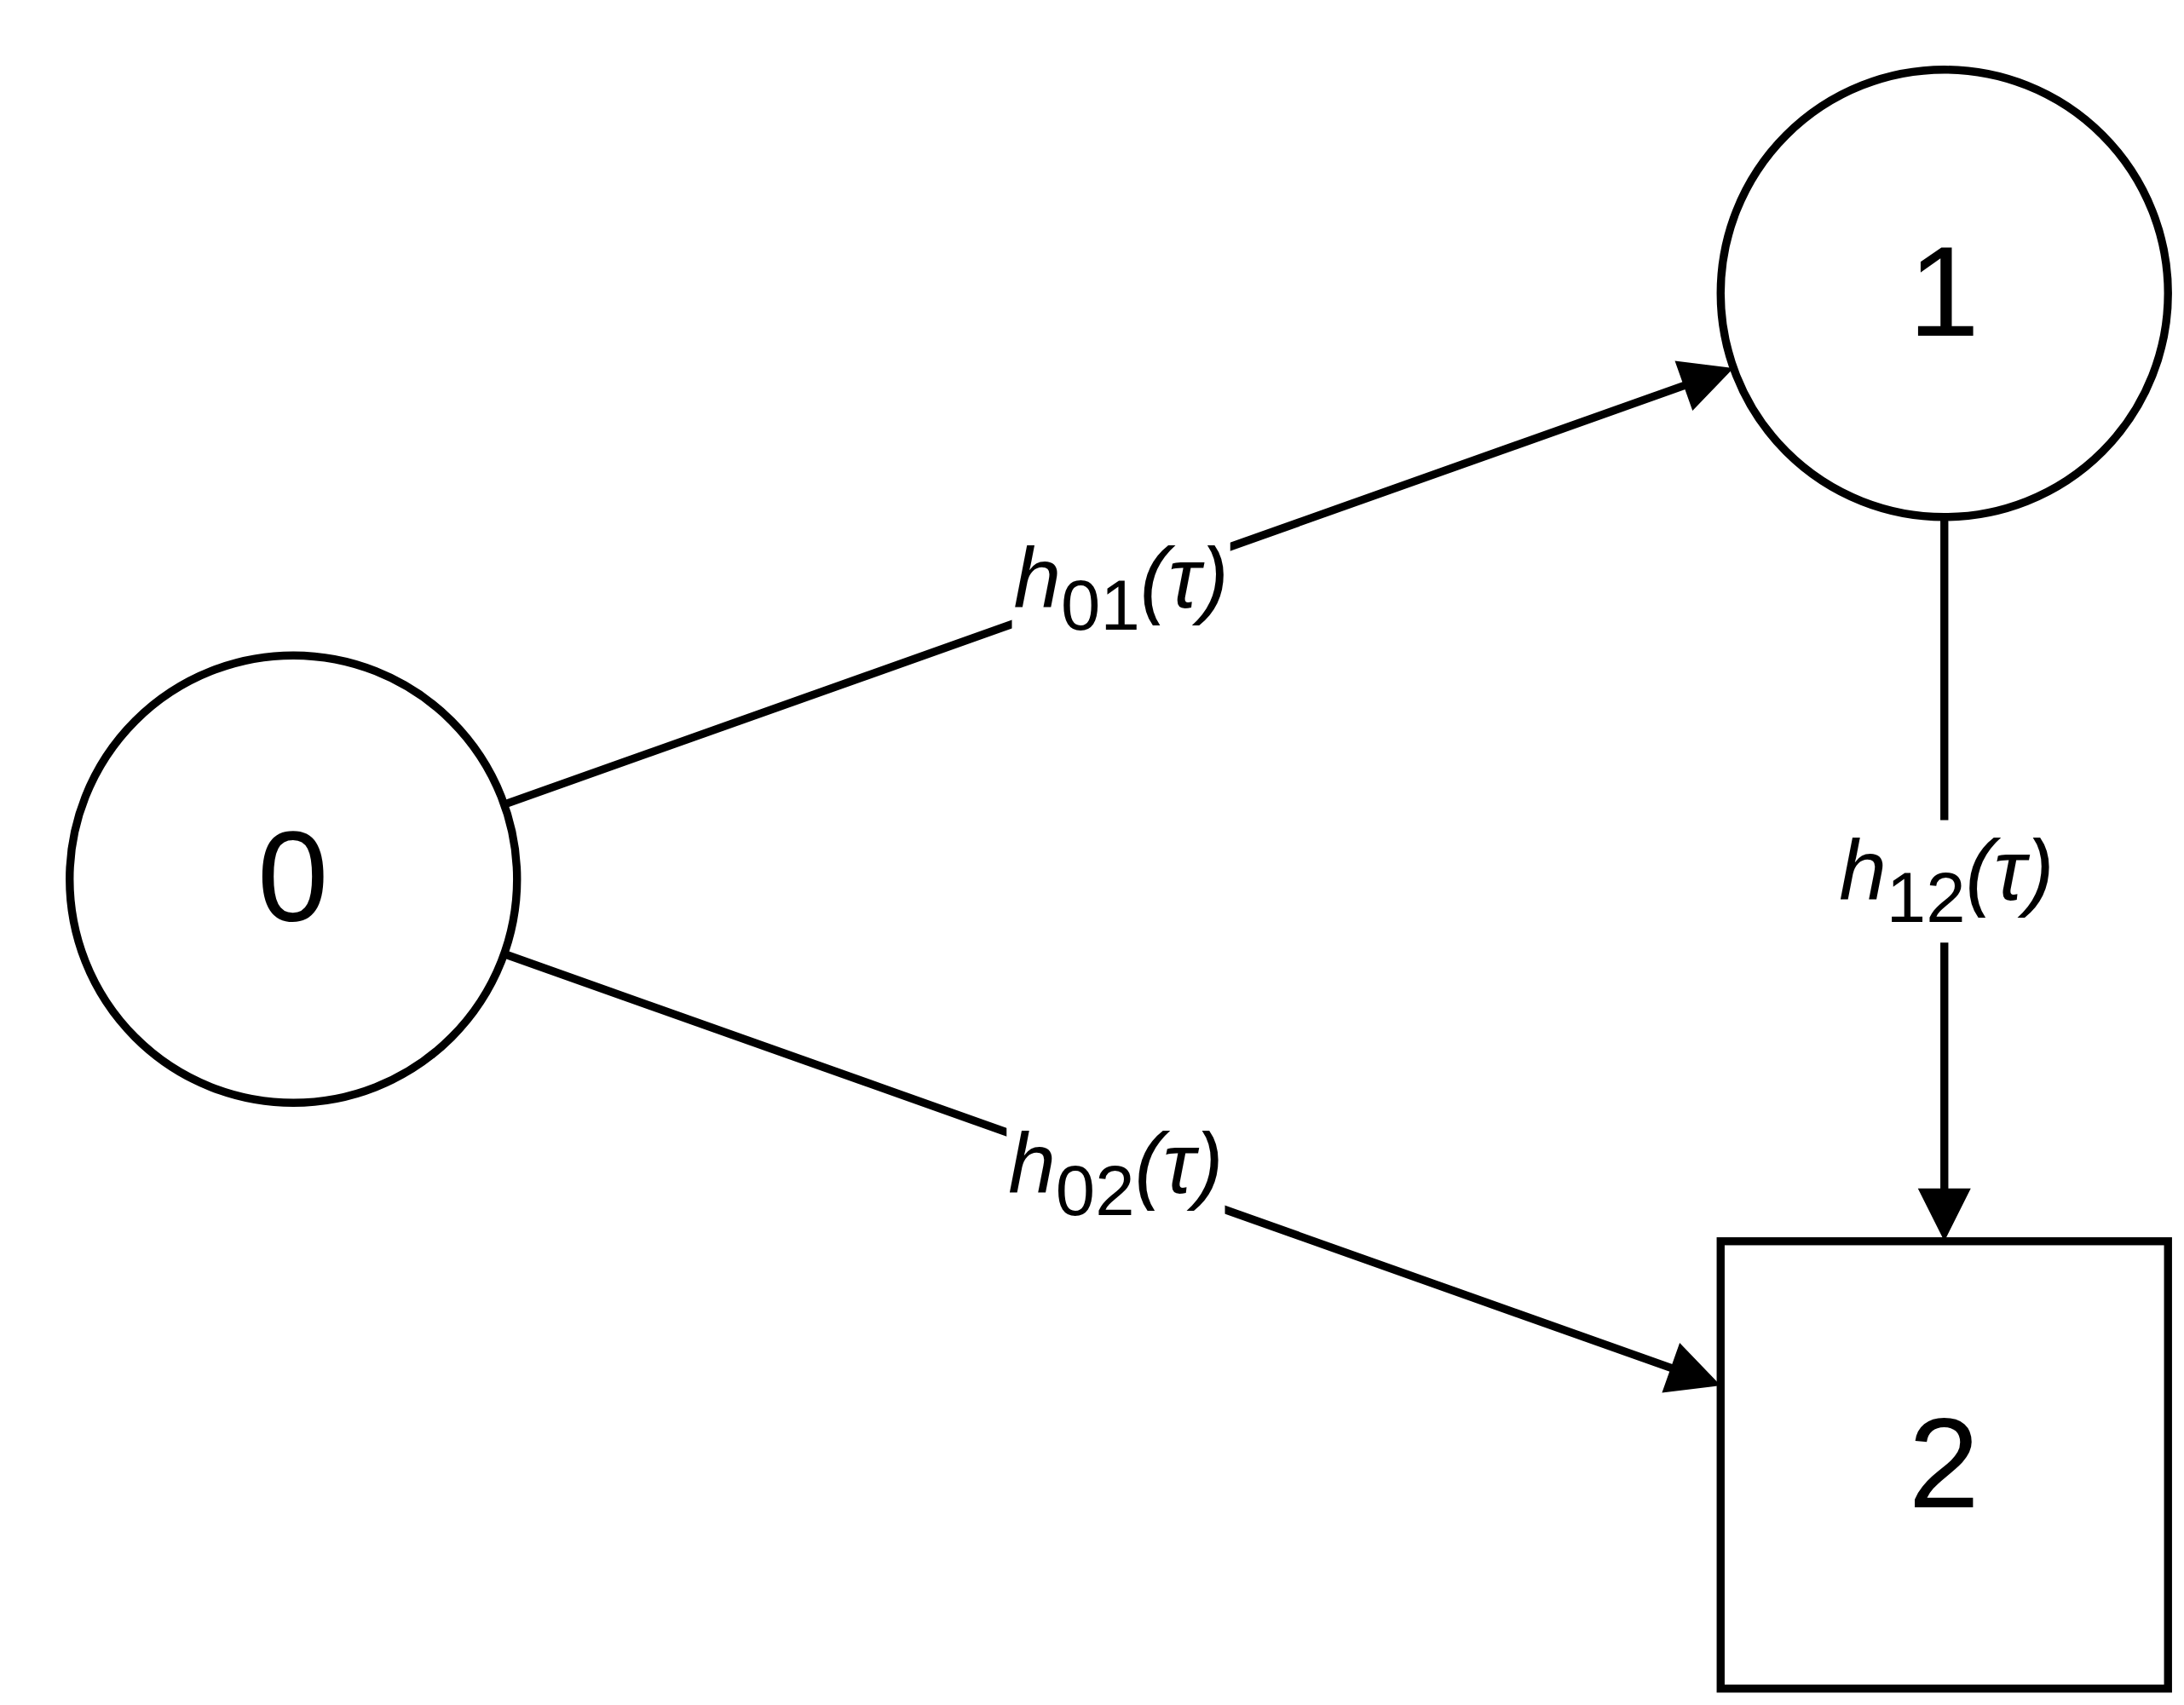
\includegraphics[width=0.6\linewidth,height=\textheight,keepaspectratio]{Figures/survival/fig-p1c5-illness-death-model.png}

}

\caption{\label{fig-p1c5-illness-death-model}An \emph{illness-death
model} where subjects can transition from healthy state (\(0\)) to death
(\(2\)) directly or via intermediate illness state (\(1\))}

\end{figure}%

In this example, back-transitions are not possible, therefore the lower
triangle of the matrix is filled with zeros and
\(P_{22}(\zeta, \tau) = 1, \forall\ \zeta < \tau\) by virtue of being a
terminal state. The matrix of transition probabilities is thus,
\begin{equation}\phantomsection\label{eq-ms-trans-prob-mat-illness-death}{
\mathbf{P}(\zeta, \tau) =
  \begin{pmatrix}
  P_{00}(\zeta, \tau) & P_{01}(\zeta, \tau) & P_{02}(\zeta, \tau)\\
  0 & P_{11}(\zeta, \tau) & P_{12}(\zeta, \tau)\\
  0 & 0 & 1\\
  \end{pmatrix}.
}\end{equation}

Assume that data is collected in discrete time, that is
\(\zeta, \tau \in \{0, 1, 2,\ldots\}, \zeta < \tau\) and transitions
only occur at these discrete time points and not in between. Say one is
interested in the transition probability \(P_{02}(4, 6)\), which is the
probability to transition from state \(0\) to state \(2\) between time
points \(\zeta=4\) and \(\tau=6\). This is possible in the three ways
depicted in Figure~\ref{fig-p1c5-example-transitions-prothr-graph}.

\begin{figure}

\centering{

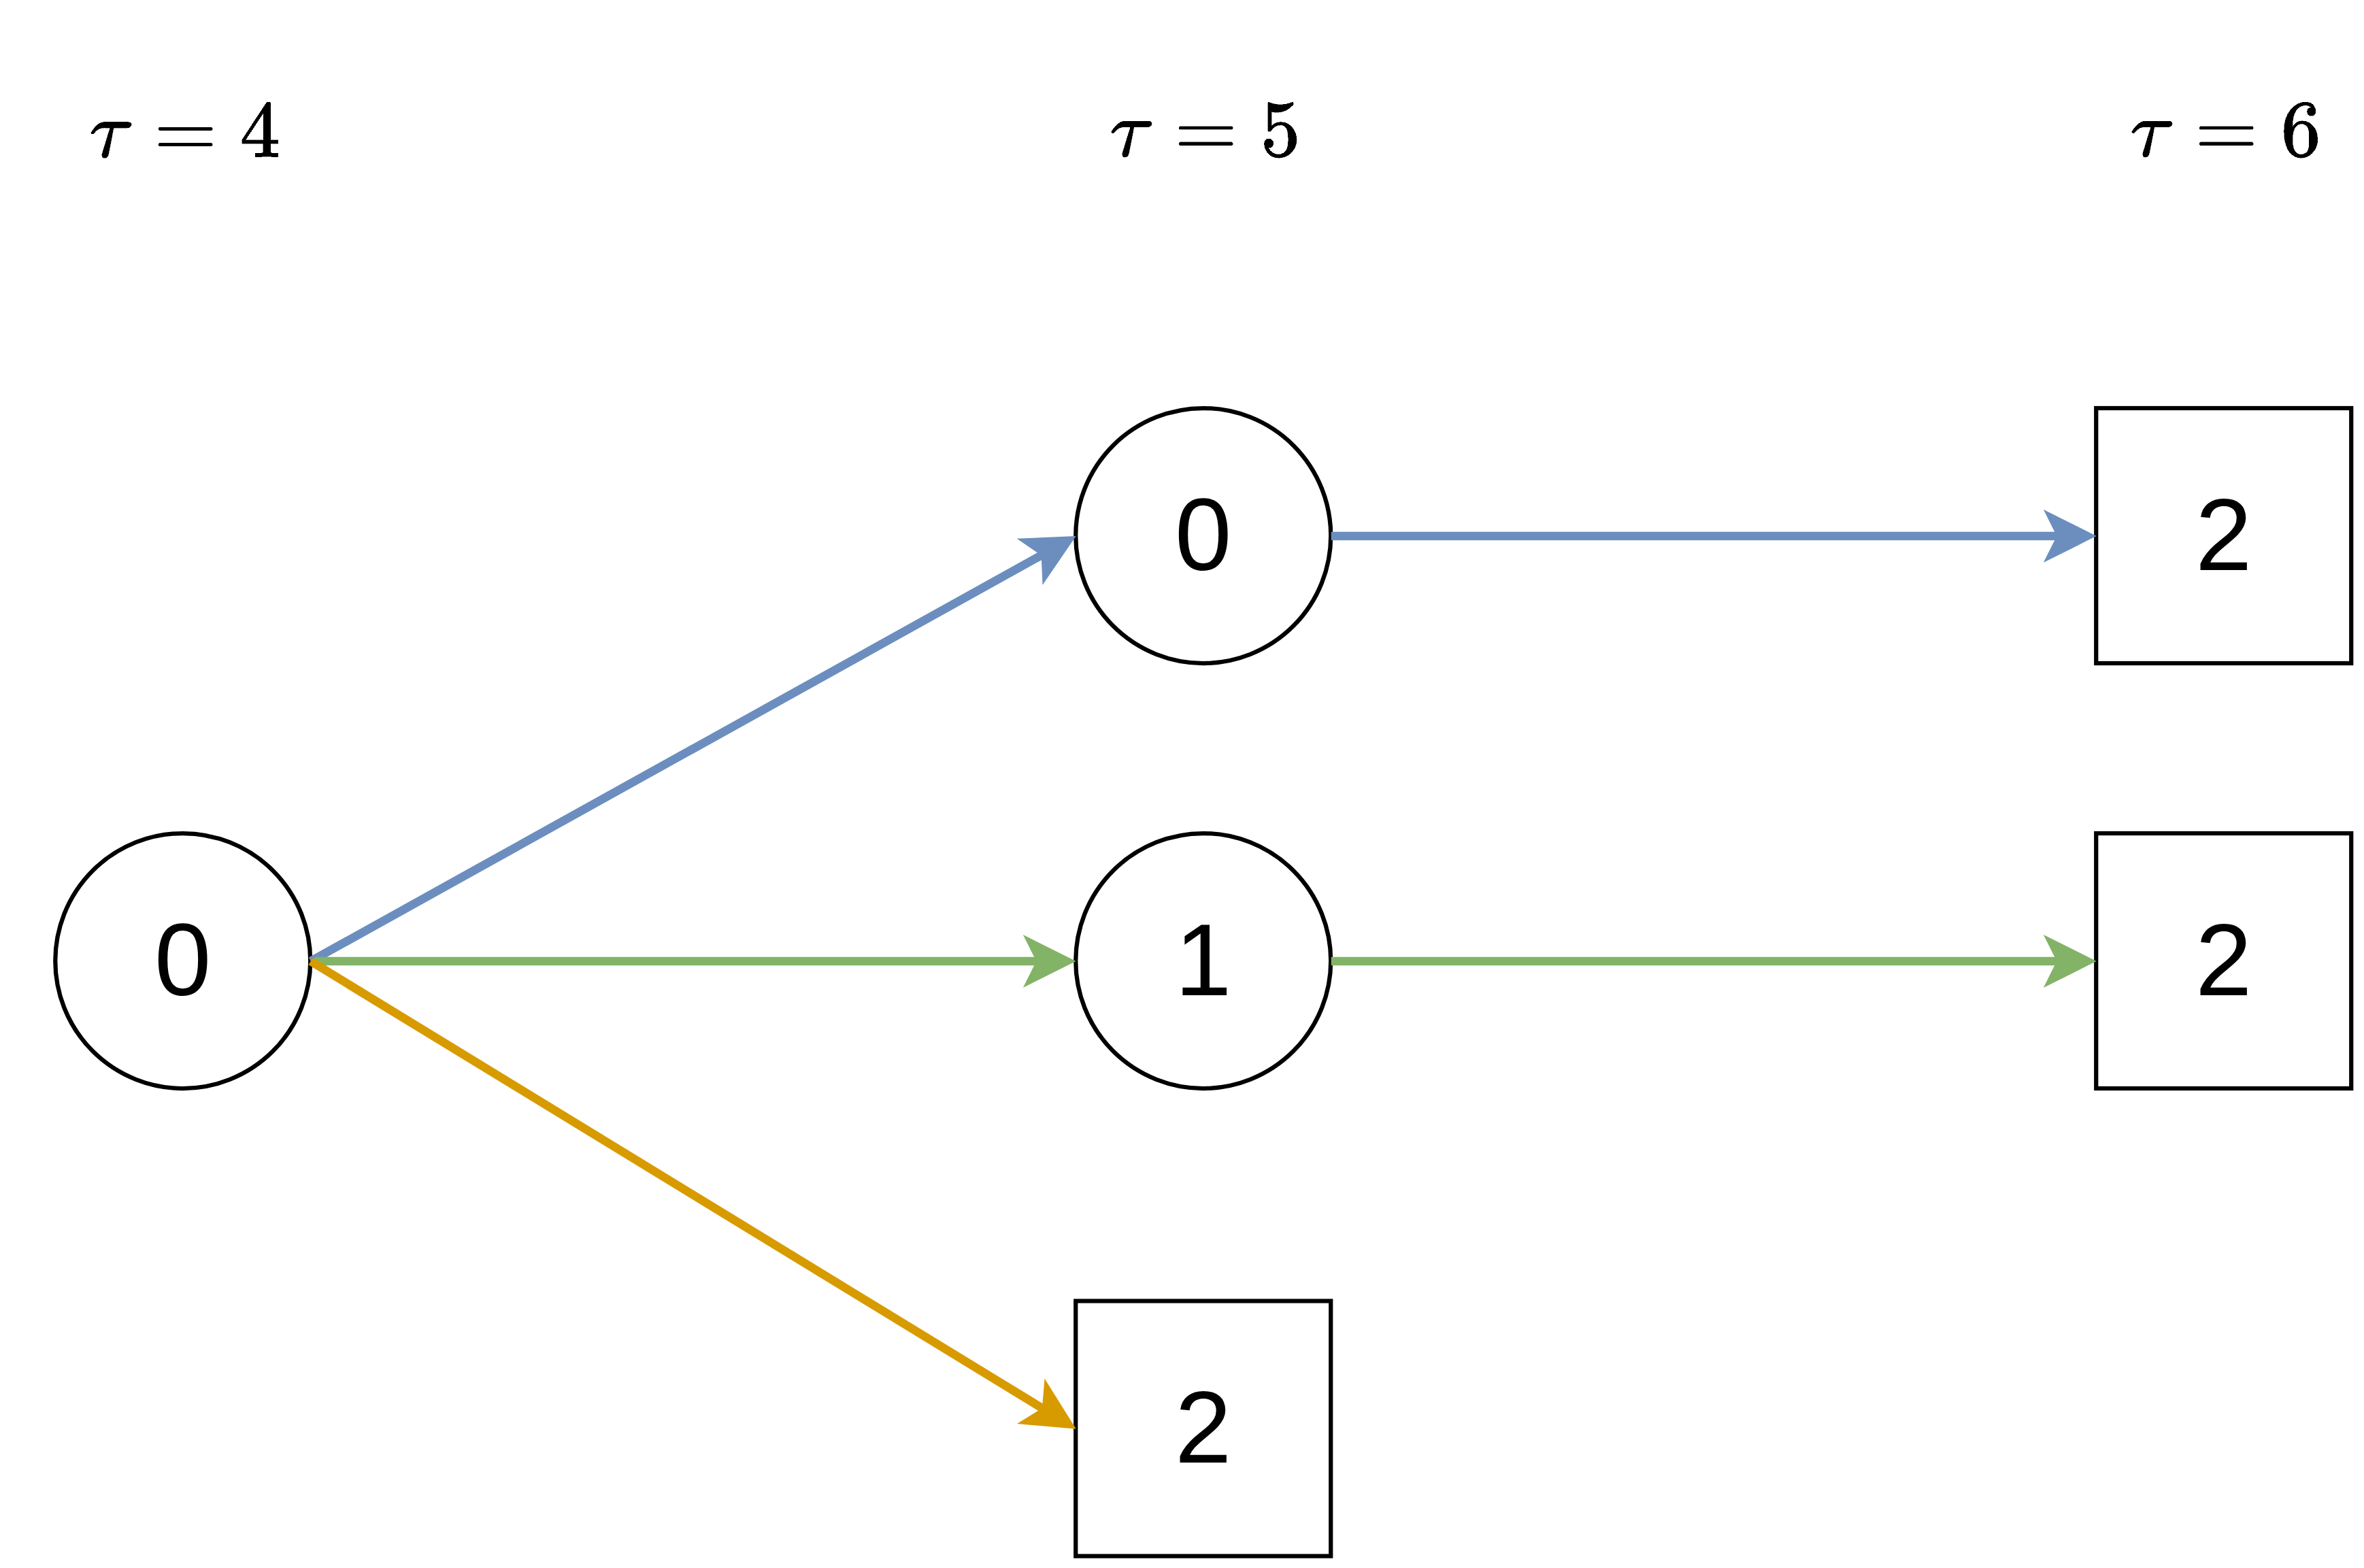
\includegraphics[width=0.8\linewidth,height=\textheight,keepaspectratio]{Figures/survival/fig-p1c5-example-transitions-prothr-graph.png}

}

\caption{\label{fig-p1c5-example-transitions-prothr-graph}Possible paths
to transition from state \(0\) to state \(2\) between time points 4 and
6.}

\end{figure}%

Let \(p_{\ell q}\) be the step probabilities for transitions
\(\ell \rightarrow q\) between two subsequent discrete time points,

\[
p_{\ell q}(\tau) = \Pr(E(\tau)=q \mid E(\tau -1) = \ell).
\]

The transition probability can then be written as,

\[
P_{02}(4,6) = \textcolor{blue}{p_{00}(5)p_{02}(6)} + \textcolor{green}{p_{01}(5)p_{12}(6)} + \textcolor{orange}{p_{02}(5)}.
\]

More generally, in discrete time, the matrix of transition probabilities
can be represented as a finite matrix product,

\begin{equation}\phantomsection\label{eq-ms-trans-prob-ill-death-discrete}{
\mathbf{P}(\zeta, \tau) = \prod_{j =\zeta+1}^{\tau}
\begin{pmatrix}
  p_{00}(j) & p_{01}(j) & p_{02}(j)\\
  0 & p_{11}(j) & p_{12}(j)\\
  0 & 0 & 1\\
  \end{pmatrix}.
}\end{equation}

For the transitions from time points \(4\) to \(6\),

\[
\begin{aligned}
\mathbf{P}(4, 6) &=
\begin{pmatrix}
P_{00}(4, 6) & P_{01}(4, 6) & P_{02}(4, 6)\\
        0 & P_{11}(4, 6) & P_{12}(4,6)\\
        0 &         0 &         1
\end{pmatrix} \\
&= \prod_{j=5}^6
\begin{pmatrix}
p_{00}(j) & p_{01}(j) & p_{02}(j)\\
        0 & p_{11}(j) & p_{12}(j)\\
        0 &         0 &         1
\end{pmatrix}\\
            & =
\begin{pmatrix}
p_{00}(5) & p_{01}(5) & p_{02}(5)\\
        0 & p_{11}(5) & p_{12}(5)\\
        0 &         0 &         1
\end{pmatrix}
\begin{pmatrix}
p_{00}(6) & p_{01}(6) & p_{02}(6)\\
        0 & p_{11}(6) & p_{12}(6)\\
        0 &         0 &         1
\end{pmatrix}\\
            &=
\begin{pmatrix}
p_{00}(5) p_{00}(6) & p_{00}(5)p_{01}(6) + p_{01}(5)p_{11}(6) & p_{00}(5)p_{02}(6) + p_{01}(5)p_{12}(6) + p_{02}(5)\\
        0           & p_{11}(5) p_{11}(6)& p_{11}(5)p_{12}(6) + p_{12}(5)\\
        0           &                  0 &         1
\end{pmatrix},
\end{aligned}
\]

where the quantity of interest, \(P_{02}(4, 6)\) is given in the top
right corner, but other transition probabilities are also readily
available. For example, the probability to transition from state \(1\)
to \(2\) between time points \(\zeta=4\) and \(\tau=6\) is
\(P_{12}(4, 6) = p_{11}(5)p_{12}(6) + p_{12}(5)\).

Returning to the continuous time setting, where transitions can occur at
any time point, ideas from the discrete time setting still hold. Imagine
dividing the interval \((\zeta, \tau]\) into \(J\) intervals such that
\(\zeta = t_{0} < t_{1} < \cdots < t_{j} < \cdots t_{J} = \tau\),
assuming that no events occur between time points
\(t_{j} \in \mathbb{R}_+, j=1,\ldots, J\). Then the transition
probability matrix \(\mathbf{P}(\zeta, \tau)\) takes the same product
form as in (\ref{eq-ms-trans-prob-ill-death-discrete}), with
\(p_{\ell q}(j)\) replaced by \(p_{\ell q}(t_j)\).

\subsection{Transition probabilities and
hazards}\label{transition-probabilities-and-hazards}

Increasing the number of intervals to infinity, or equivalently reducing
the interval size to infinitesimally small intervals, one can define the
transition probability matrix\index{transition probability matrix} as a
product integral over the instantaneous transition probabilities
\(p_{\ell q}(u)\), expressed in terms of transition-specific
(cumulative) hazards.

First note from equations (\ref{eq-ms-transition-hazards}) and
(\ref{eq-ms-cumu-hazard}) that the instantaneous transition
probabilities can be approximated by increments of the cumulative
hazard, which is the increase in the cumulative hazard within a fixed,
infinitesimally small interval \(\,\mathrm{d}u\): \[
p_{\ell q}(u) := \Pr\big(E(u+\mathrm{d}u)=q \mid E(u-) = \ell\big) \approx \mathrm{d}H_{\ell q}(u).
\]

Secondly, because of the relationship in
(\ref{eq-ms-trans-prob-row-sums}), diagonal elements (transitions into
the same state) are set to,

\[
\mathrm{d}H_{\ell \ell}(u) := -\sum_{q \neq \ell} \mathrm{d}H_{\ell q}(u),
\]

such that

\[
1 + \mathrm{d}H_{\ell\ell}(u) = 1-\sum_{q \neq \ell} \mathrm{d}H_{\ell q}(u) = 1 - \sum_{q\neq \ell}p_{\ell q}(u) = p_{\ell\ell}(u).
\]

Consequently, the transition probability matrix can be written as,

\begin{equation}\phantomsection\label{eq-ms-prodint-cumu-hazards}{
\begin{aligned}
\mathbf{P}(\zeta, \tau)
                        &= \mathscr{P}_{u \in (\zeta, \tau]}
  \begin{pmatrix}
    p_{00}(u) = 1 + \mathrm{d}H_{00}(u) & \cdots & p_{0Q}(u) = \mathrm{d}H_{0Q}(u)\\
    \vdots                  & \ddots & \vdots\\
    p_{Q0}(u) =  \mathrm{d}H_{Q0}(u)     & \cdots & p_{QQ}(u) = 1 + \mathrm{d}H_{QQ}(u)\\
  \end{pmatrix}\\
  & \ \\
  & =  \mathscr{P}_{u \in (\zeta, \tau]}(\mathbf{I} + \mathrm{d}\mathbf{H}(u)),\\
\end{aligned}
}\end{equation}

where \(\mathscr{P}\) is the product integral operator, \(\mathbf{I}\)
is a \((Q+1) \times (Q+1)\) identity matrix and
\(\mathrm{d}\mathbf{H}(u)\) is the matrix of increments of the
cumulative hazard within infinitesimally small intervals. Thus, similar
to the competing risks setting\index{competing risks}, the relationship
(\ref{eq-ms-prodint-cumu-hazards}) implies that knowledge of the
transition (cumulative) hazards is sufficient to fully specify the
multi-state process.

As analytical solutions of (\ref{eq-ms-prodint-cumu-hazards}) only exist
for specific models, in practice, the transition probabilities are often
once again approximated numerically via a finite matrix product on a
discrete time grid
\(\zeta = t_0 < t_1 < \cdots < t_{J-1} < t_{J} = \tau\),
\begin{equation}\phantomsection\label{eq-ms-prodint-approx}{
\mathbf{P}(\zeta, \tau) \approx \prod_{j=1}^{J}(\mathbf{I} + \triangle\mathbf{H}(t_{j})),
}\end{equation} where
\(\triangle \mathbf{H}(t_{j}) = \mathbf{H}(t_{j}) - \mathbf{H}(t_{j-1})\)
is the increment of the cumulative hazards between two consecutive time
points.

\subsection{Non-parametric estimation of transition
probabilities}\label{sec-ms-aalen-johansen}

From (\ref{eq-ms-prodint-approx}), it follows that transition
probabilities can be estimated by first computing the transition
cumulative hazards\index{transition cumulative hazard function},
\(H_{\ell q}(\tau)\). Similarly to the AJ approach in the competing
risks setting (Section~\ref{sec-aalen-johansen})
\index{Aalen-Johansen estimator}, one can first define the
\emph{transition hazards}\index{transition hazard function},

\[
h^{d}_{\ell q}(t_{(k)}):= \frac{d_{\ell q,t_{(k)}}}{n_{\ell; t_{(k)}}},
\]

where \(d_{\ell q,t_{(k)}}\) is the number of subjects that made the
transition \(\ell \rightarrow q\) at time \(t_{(k)}\); and
\(n_{\ell; t_{(k)}}\) is the number of subjects in state \(\ell\)
immediately before \(t_{(k)}\).

The \emph{transition cumulative hazards} follow
as\index{transition cumulative hazard function} \[
H_{AJ,\ell q}(\tau) = \sum_{k:t_{(k)}\leq \tau} h^d_{\ell q}(t_{(k)}) = \sum_{k:t_{(k)}\leq \tau}\frac{d_{\ell q,t_{(k)}}}{n_{\ell; t_{(k)}}},
\]

Transition probabilities\index{transition probability} are obtained via
(\ref{eq-ms-prodint-approx}),
\begin{equation}\phantomsection\label{eq-ms-aj-trans-prob}{
\mathbf{P}(\zeta, \tau) = \prod_{j=1}^{J}\left(\mathbf{I} + \triangle\mathbf{H}_{AJ}(t_{(j)})\right).
}\end{equation}

\subsection{State occupation
probabilities}\label{sec-ms-state-occupation}

The pairwise transition probabilities, \(P_{\ell q}(\zeta, \tau)\),
defined above are conditioned on a specific entry-state \(\ell\) at a
specific time \(\zeta\); the Aalen-Johansen estimator
(\ref{eq-ms-aj-trans-prob}) is only consistent for them under the
Markov\index{Markov} assumption. A closely related but conceptually
distinct target is the \emph{state-occupation
probability}\index{state-occupation probability},
\begin{equation}\phantomsection\label{eq-ms-state-occupation}{
P_q(\tau) := \Pr(E(\tau) = q),
}\end{equation} which is the marginal probability that a subject
occupies state \(q\) at time \(\tau\).

State-occupation probabilities are arguably the more natural target for
many prediction tasks: questions of the form ``what is the probability
that the subject is alive in normal-prothrombin state at \(\tau = 365\)
days?'' are directly answered by \(P_q(\tau)\), not by a pairwise
transition probability conditioned on a fixed entry-state.

An important property is that the Aalen-Johansen plug-in
(\ref{eq-ms-aj-trans-prob}), applied with the empirical initial-state
distribution rather than conditioned on a fixed \(\ell\), remains a
consistent estimator of \(P_q(\tau)\) even when the underlying process
is not Markov (Nießl et al. 2023; Putter and Spitoni 2018).

Concretely, given the AJ estimate \(\widehat{\mathbf{P}}(0, \tau)\) and
the empirical initial-state distribution
\(\hat{\pi}_\ell = n_\ell^{(0)}/n\) (where \(n_\ell^{(0)}\) is the
number of subjects observed in state \(\ell\) at \(\tau=0\)), the
state-occupation estimator is
\begin{equation}\phantomsection\label{eq-ms-state-occupation-est}{
\hat{P}_{AJ,q}(\tau) = \sum_{\ell=0}^{Q} \hat{\pi}_\ell\, \widehat{P}_{\ell q}(0, \tau).
}\end{equation} The final section below reports the pairwise transition
probabilities under the Markov assumption. Deriving the state-occupation
estimates follows by applying the same AJ pipeline and then
marginalizing with (\ref{eq-ms-state-occupation-est}).

\subsection{Application to liver cirrhosis
patients}\label{application-to-liver-cirrhosis-patients}

For illustration, consider again the \texttt{prothr} data set
(Table~\ref{tbl-ms-data-prothr}), with possible transitions summarized
in Figure~\ref{fig-p1c5-multi-state-prothr-states}. In contrast to the
illness-death model in Figure~\ref{fig-p1c5-illness-death-model}, back
transitions are possible and some subjects already start in the abnormal
prothrombin state at the beginning of the study.

The estimands of interest are the four off-diagonal transition
probabilities \(\hat{P}_{\ell q}(0, \tau)\) for
\((\ell, q) \in \{(0,1), (0,2), (1,0), (1,2)\}\), computed separately
for the prednisone and placebo arms via the Aalen-Johansen
estimator\index{Aalen-Johansen estimator} (\ref{eq-ms-aj-trans-prob}).
Stratifying by treatment treats each arm as a homogeneous Markov
sub-population, with no further covariate adjustment. This is a coarse
but standard simplification; regression-based extensions that
incorporate subject-level features into the multi-state estimation are
taken up later in the book.

Figure~\ref{fig-p1c5-multi-state-prothr} shows these probabilities for
both arms. In contrast to the cumulative incidence
functions\index{cumulative incidence function} of the competing-risks
setting (Section~\ref{sec-aalen-johansen}), the curves targeting
\emph{transient} states\index{transient states} (such as
\(\ell \rightarrow 0\) and \(\ell \rightarrow 1\)) are not monotonically
increasing in \(\tau\). This is a feature of the underlying mathematics,
the terminal state mass \(P_{\ell 2}(0, \tau)\) grows monotonically with
\(\tau\) and the row-sum constraint (\ref{eq-ms-trans-prob-row-sums})
forces the transient-state probabilities to give up mass to compensate.

The curves for \(0 \rightarrow 2\) and \(1 \rightarrow 2\) (death)
increase monotonically over follow-up in both arms, as expected for
terminal-state probabilities. Relative to the placebo, between days
\(1,000\) and \(3,000\), the prednisone arm shows a modest reduction in
the \(0 \rightarrow 2\) transition probability and an increase in the
back-transition \(1\rightarrow 0\), but the gap narrows toward the end
of follow-up. The overall conclusion is that prednisone does not appear
to confer a strong, persistent protective effect. Meaningful inference
about treatment effects would require accompanying uncertainty bands and
is beyond the descriptive scope of this stratified Aalen-Johansen
analysis.

\begin{figure}

\centering{

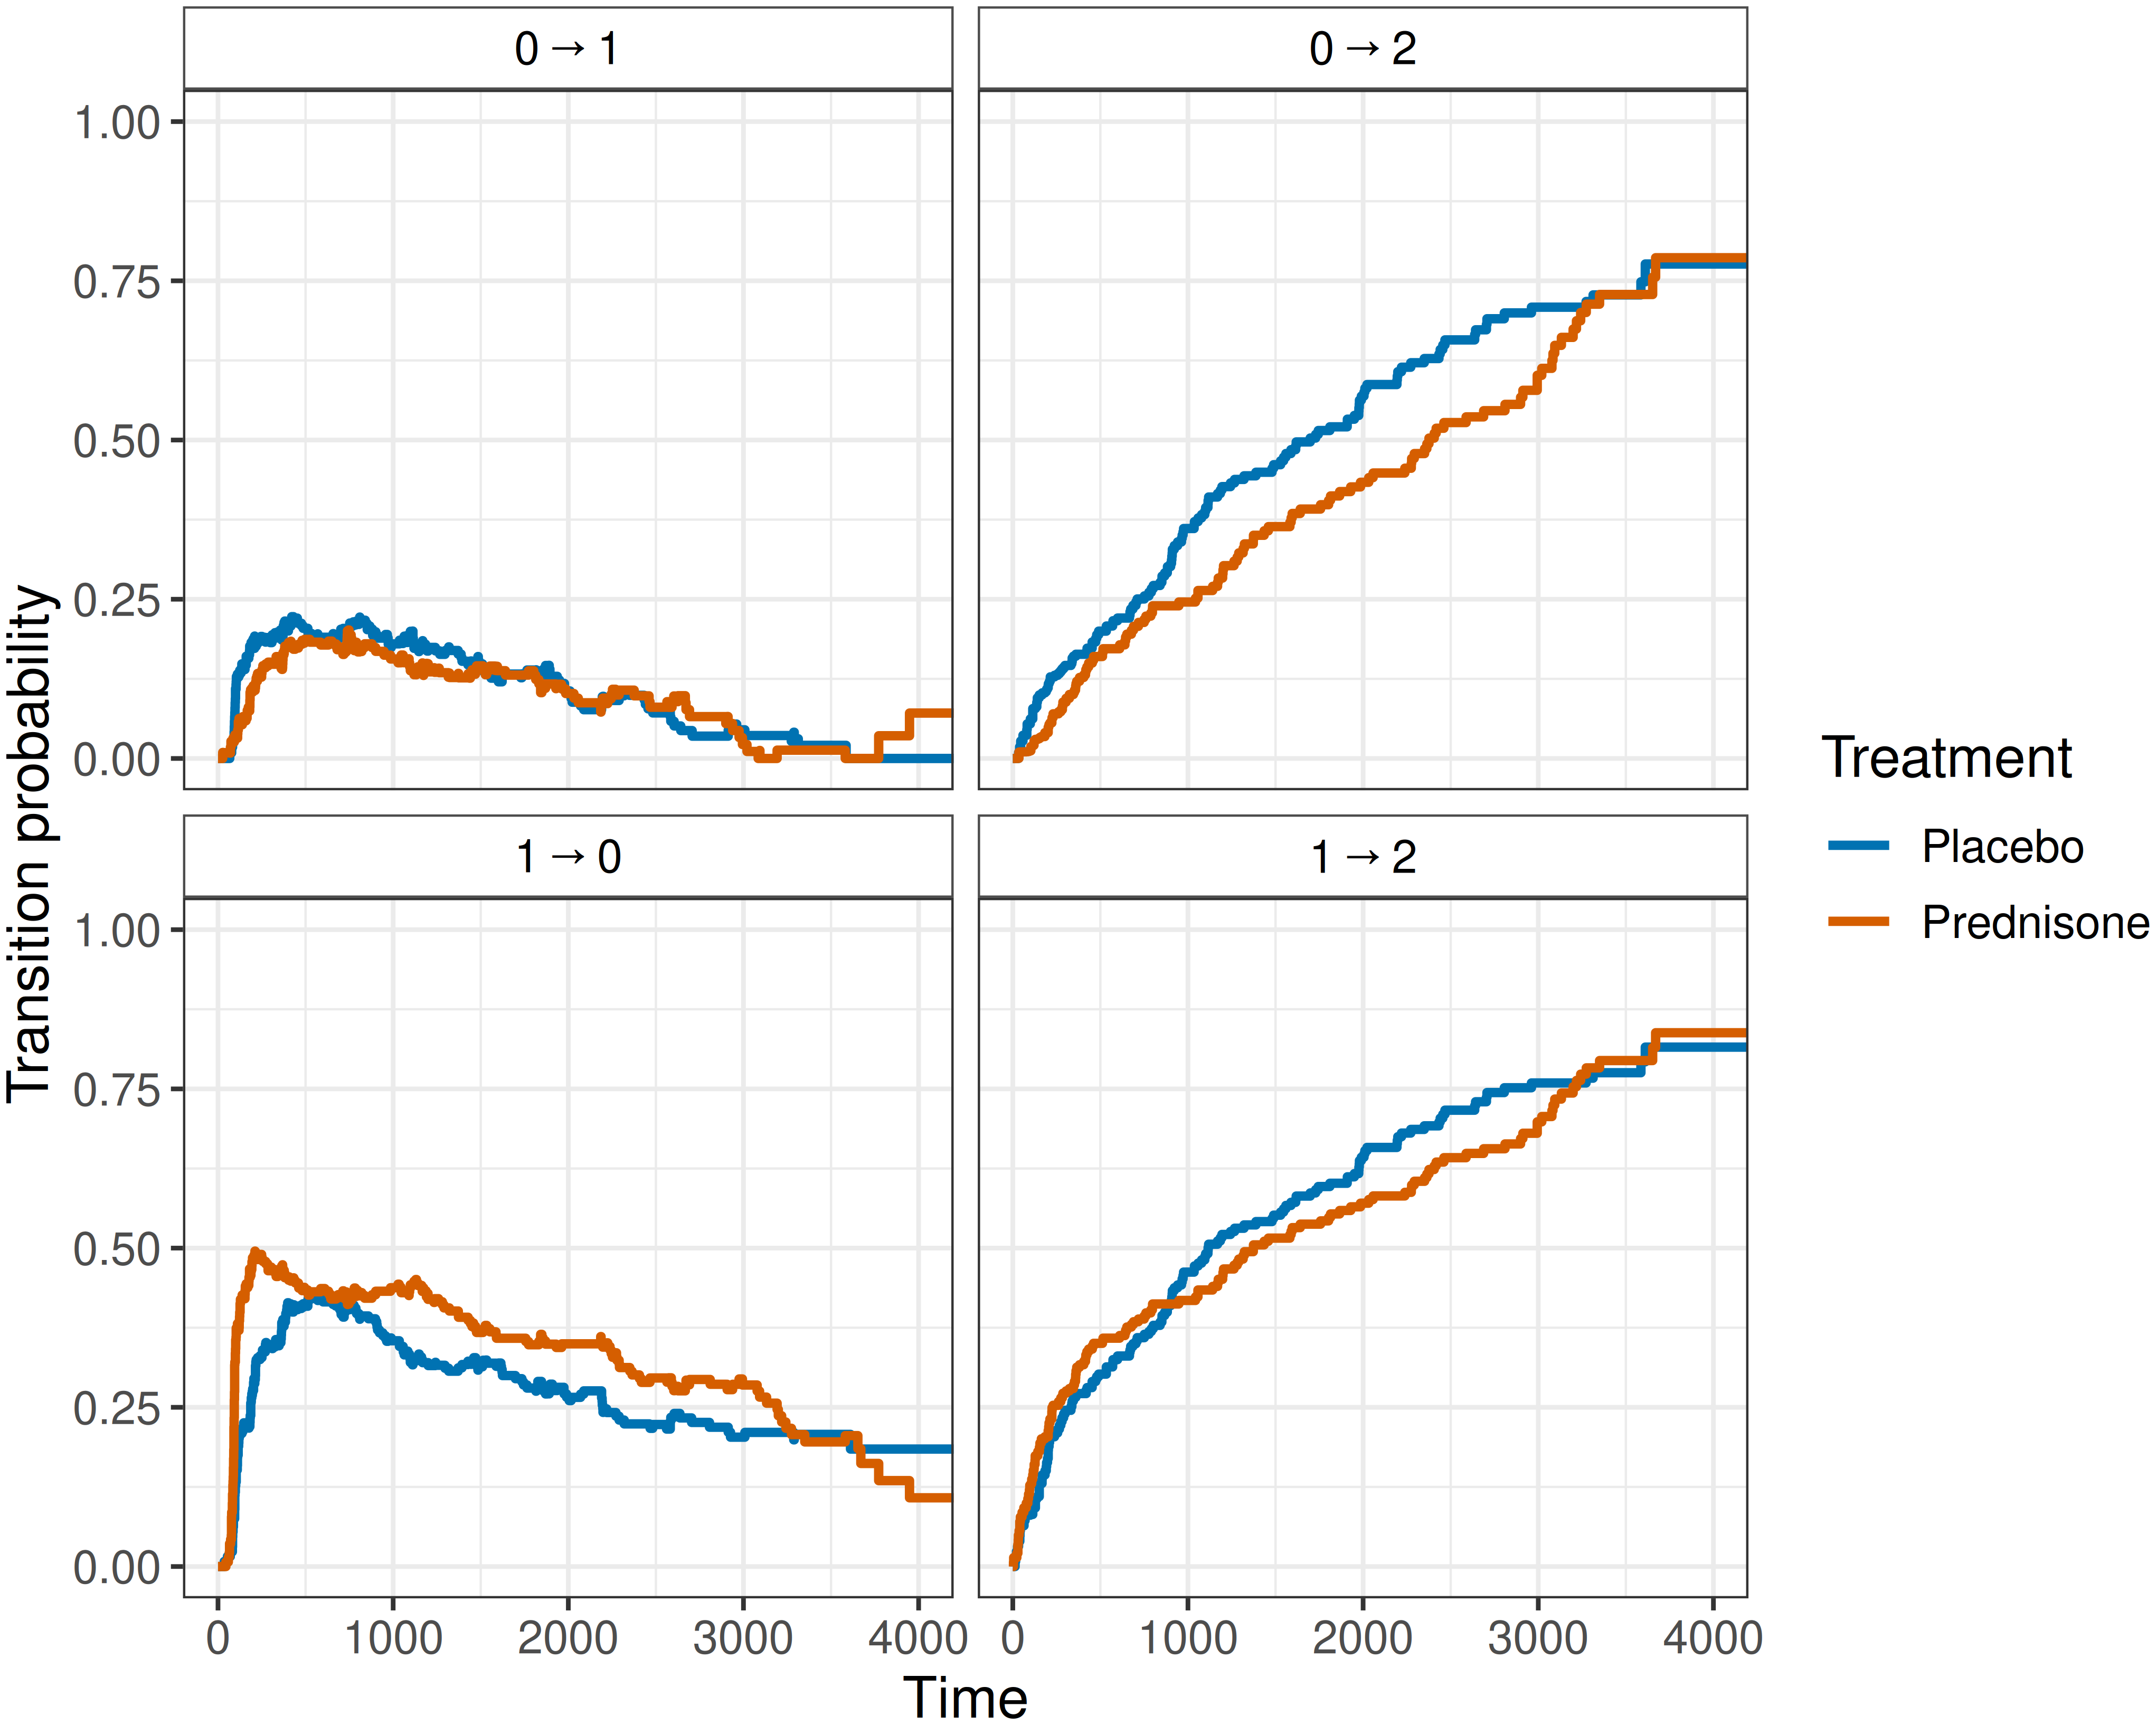
\includegraphics[width=1\linewidth,height=\textheight,keepaspectratio]{Figures/survival/fig-p1c5-multi-state-prothr.png}

}

\caption{\label{fig-p1c5-multi-state-prothr}Estimated transition
probabilities for the different transitions of the prothrombin data
example. Top-left: transition from normal levels to abnormal. Top-right:
transition from normal levels to death. Bottom-left: transition from
abnormal levels to normal. Bottom-right: transition from abnormal levels
to death. Blue curves are placebo, orange are prednisone.}

\end{figure}%

\section{Conclusion}\label{conclusion-2}

\begin{tcolorbox}[enhanced jigsaw, toprule=.15mm, bottomtitle=1mm, opacityback=0, breakable, leftrule=.75mm, title={Key takeaways}, toptitle=1mm, bottomrule=.15mm, colback=white, colframe=quarto-callout-warning-color-frame, titlerule=0mm, opacitybacktitle=0.6, coltitle=black, rightrule=.15mm, left=2mm, colbacktitle=quarto-callout-warning-color!10!white, arc=.35mm]

\begin{itemize}
\tightlist
\item
  Event history analysis generalizes the standard survival analysis
  setting by representing subjects as moving between states over time,
  allowing competing, recurrent, and multi-state outcomes to be modeled
  within a common framework.
\item
  In competing-risks settings, treating competing events as independent
  censoring can substantially distort estimated event probabilities;
  cumulative incidence functions and the Aalen-Johansen estimator
  account for this dependence explicitly.
\item
  Multi-state processes are characterized through transition hazards and
  transition probabilities, with the Aalen-Johansen estimator providing
  a non-parametric plug-in estimator based on estimated transition
  hazards and product integrals.
\item
  Defining the state diagram of the data generating process can be a
  helpful first step to understand the dynamics in the data and to
  select an appropriate framework (and model) for the analysis.
\end{itemize}

\end{tcolorbox}

\begin{tcolorbox}[enhanced jigsaw, toprule=.15mm, bottomtitle=1mm, opacityback=0, breakable, leftrule=.75mm, title={Further reading}, toptitle=1mm, bottomrule=.15mm, colback=white, colframe=quarto-callout-tip-color-frame, titlerule=0mm, opacitybacktitle=0.6, coltitle=black, rightrule=.15mm, left=2mm, colbacktitle=quarto-callout-tip-color!10!white, arc=.35mm]

\begin{itemize}
\tightlist
\item
  Aalen, Borgan, and Gjessing (2008) introduces different approaches for
  event history analysis motivated from the counting process point of
  view.
\item
  Beyersmann, Allignol, and Schumacher (2012) provide an accessible
  overview of important concepts for competing risks and multi-state
  modeling, particularly non-parametric estimation.
\end{itemize}

\end{tcolorbox}

\chapter{Survival Task}\label{sec-survtsk}

A machine learning task\index{machine learning task} specifies a
mathematical problem to be solved by an algorithm\index{algorithm}
(Section~\ref{sec-ml-tasks}). Formally, a task is a mapping
\(g: \mathcal{X}\rightarrow \mathcal{Y}\) with three components: a
description of the input space \(\mathcal{X}\), a description of the
target space \(\mathcal{Y}\), and a description of the estimation
procedure that learns \(g\) from data. A \emph{survival
task}\index{machine learning task!survival} is a machine learning task
in which the target space \(\mathcal{Y}_S\) corresponds to a
\emph{survival prediction type}\index{prediction types}
(Section~\ref{sec-surv-tsk-predicts}), and the learning algorithm is
designed to handle censoring and/or truncation while targeting that
prediction type (as in the methods introduced in Part III).

Throughout this chapter, let \(\mathcal{X}\subseteq \mathbb{R}^p\) be
the feature space. The censoring mechanism does not affect the
definition of the prediction types, hence this chapter does not
distinguish between right-, left-, or interval-censoring when defining
\(\mathcal{Y}_S\).

\section{Survival prediction types}\label{sec-surv-tsk-predicts}

A survival prediction type specifies the output space \(\mathcal{Y}_S\)
(the codomain of \(g_S\)). Four types are commonly distinguished:

\begin{enumerate}
\def\labelenumi{\arabic{enumi}.}
\tightlist
\item
  Survival distribution\index{survival distribution}: Probability of the
  event occurring over time (Section~\ref{sec-survtsk-dist});
\item
  Relative risk\index{relative risk}: A scalar quantity that represents
  the risk of the event and is meaningful only in comparison to other
  individuals in the sample (Section~\ref{sec-survtsk-risk});
\item
  Survival time or time-to-event\index{survival time}: A point
  prediction of the time at which the event of interest will occur
  (Section~\ref{sec-survtsk-time});
\item
  Prognostic index\index{prognostic index}: A risk score usually based
  on a linear predictor\index{linear predictor}
  (Section~\ref{sec-survtsk-PI}).
\end{enumerate}

Survival distribution predictions are \emph{probabilistic} as they
return a full distribution over time\index{probabilistic predictions}.
Survival time predictions are \emph{deterministic} point predictions in
the sense that they return a single scalar value, though uncertainty
remains due to underlying variance\index{deterministic predictions}.
Relative risk and prognostic index predictions do not directly predict
when or if the event of interest will occur. Instead, they produce
scores that can be used to rank or compare an individual's risk to
others in the same cohort.

The term \emph{relative} risk is used throughout this book to emphasize
that these types of predictions should only be interpreted in comparison
to others in the cohort; this is revisited in
Section~\ref{sec-survtsk-risk}. This contrasts with predictions such as
survival probability estimates, which quantify an individual's
probability of surviving to a given time point and are therefore
directly related to event risk, but remain interpretable independently.

The four prediction types are closely related. Relative risks and
survival time predictions can be derived from a predicted survival
distribution, though the reverse does not hold in general as a single
survival time or risk score does not uniquely determine a probability
distribution. Both prognostic index and time-to-event predictions can
usually be interpreted as a type of relative risk prediction. Under
(often strict) assumptions, prediction types can be converted between
one another. In fact, many algorithms appear to target a given
prediction type but internally compute another as an intermediate step.
This pattern will appear throughout Part III; for example, the
prognostic index is computed in linear models before being transformed
to a survival distribution prediction (some examples in
Chapter~\ref{sec-classical}).

Despite their close connection, it is essential to keep discussion of
prediction types distinct as they are not directly comparable. For
example, it is not meaningful to compare a relative risk score from one
model to a survival distribution prediction of another without first
transforming the distribution prediction. Even within a single
prediction type, interpretations can be confused. For example, in some
literature a larger value of a risk score implies higher risk of the
event, whereas in other sources, a larger value implies lower risk.
Distinction of prediction types is also critical for evaluation as each
prediction type naturally aligns with different types of metrics, a
topic returned to throughout Part II.

In applied predictive modeling, \emph{direct} survival time predictions
are uncommon as they can be challenging to estimate and evaluate
reliably under censoring, particularly when prediction requires
extrapolation beyond the observed follow-up period. Instead,
practitioners often report distribution-derived summaries such as
\(\tau\)-year survival
probabilities\index{t-year survival probability@$\tau$-year survival probability}
or the predicted median survival time\index{median survival time}.
Similarly, the prognostic index is less frequently used as a direct
prediction target and more commonly used for model interpretation or
inference, whereas relative risk predictions are common in applications
such as resource allocation and risk stratification. However, as
discussed below, a prognostic index can usually be interpreted as a
relative risk.

Figure~\ref{fig-p1c6-predict-types} illustrates the information provided
by the different prediction types based on a
Weibull\index{Weibull distribution} accelerated failure
time\index{accelerated failure time} model
(Section~\ref{sec-surv-models-param}). The prognostic
index\index{prognostic index} is omitted as it would appear visually
identical to the relative risk\index{relative risk} prediction type. The
top-left panel shows tabular survival data using the six patients from
the \texttt{tumor} data set (Table~\ref{tbl-surv-data-tumor}). The
top-right panel shows predicted survival times\index{survival time}, for
each observation this is a single scalar value representing the
estimated event time (here, expectation with 95\% confidence interval).
The bottom-left panel visualizes relative risk predictions; here the
score is the negative log of the predicted expected survival time,
centered at zero across the six patients, so positive values indicate
higher than average risk and negative values lower than average risk.
Finally, the bottom-right panel shows survival distribution
predictions\index{survival distribution}, where each observation's
predicted survival function is visualized over time.

\begin{figure}

\centering{

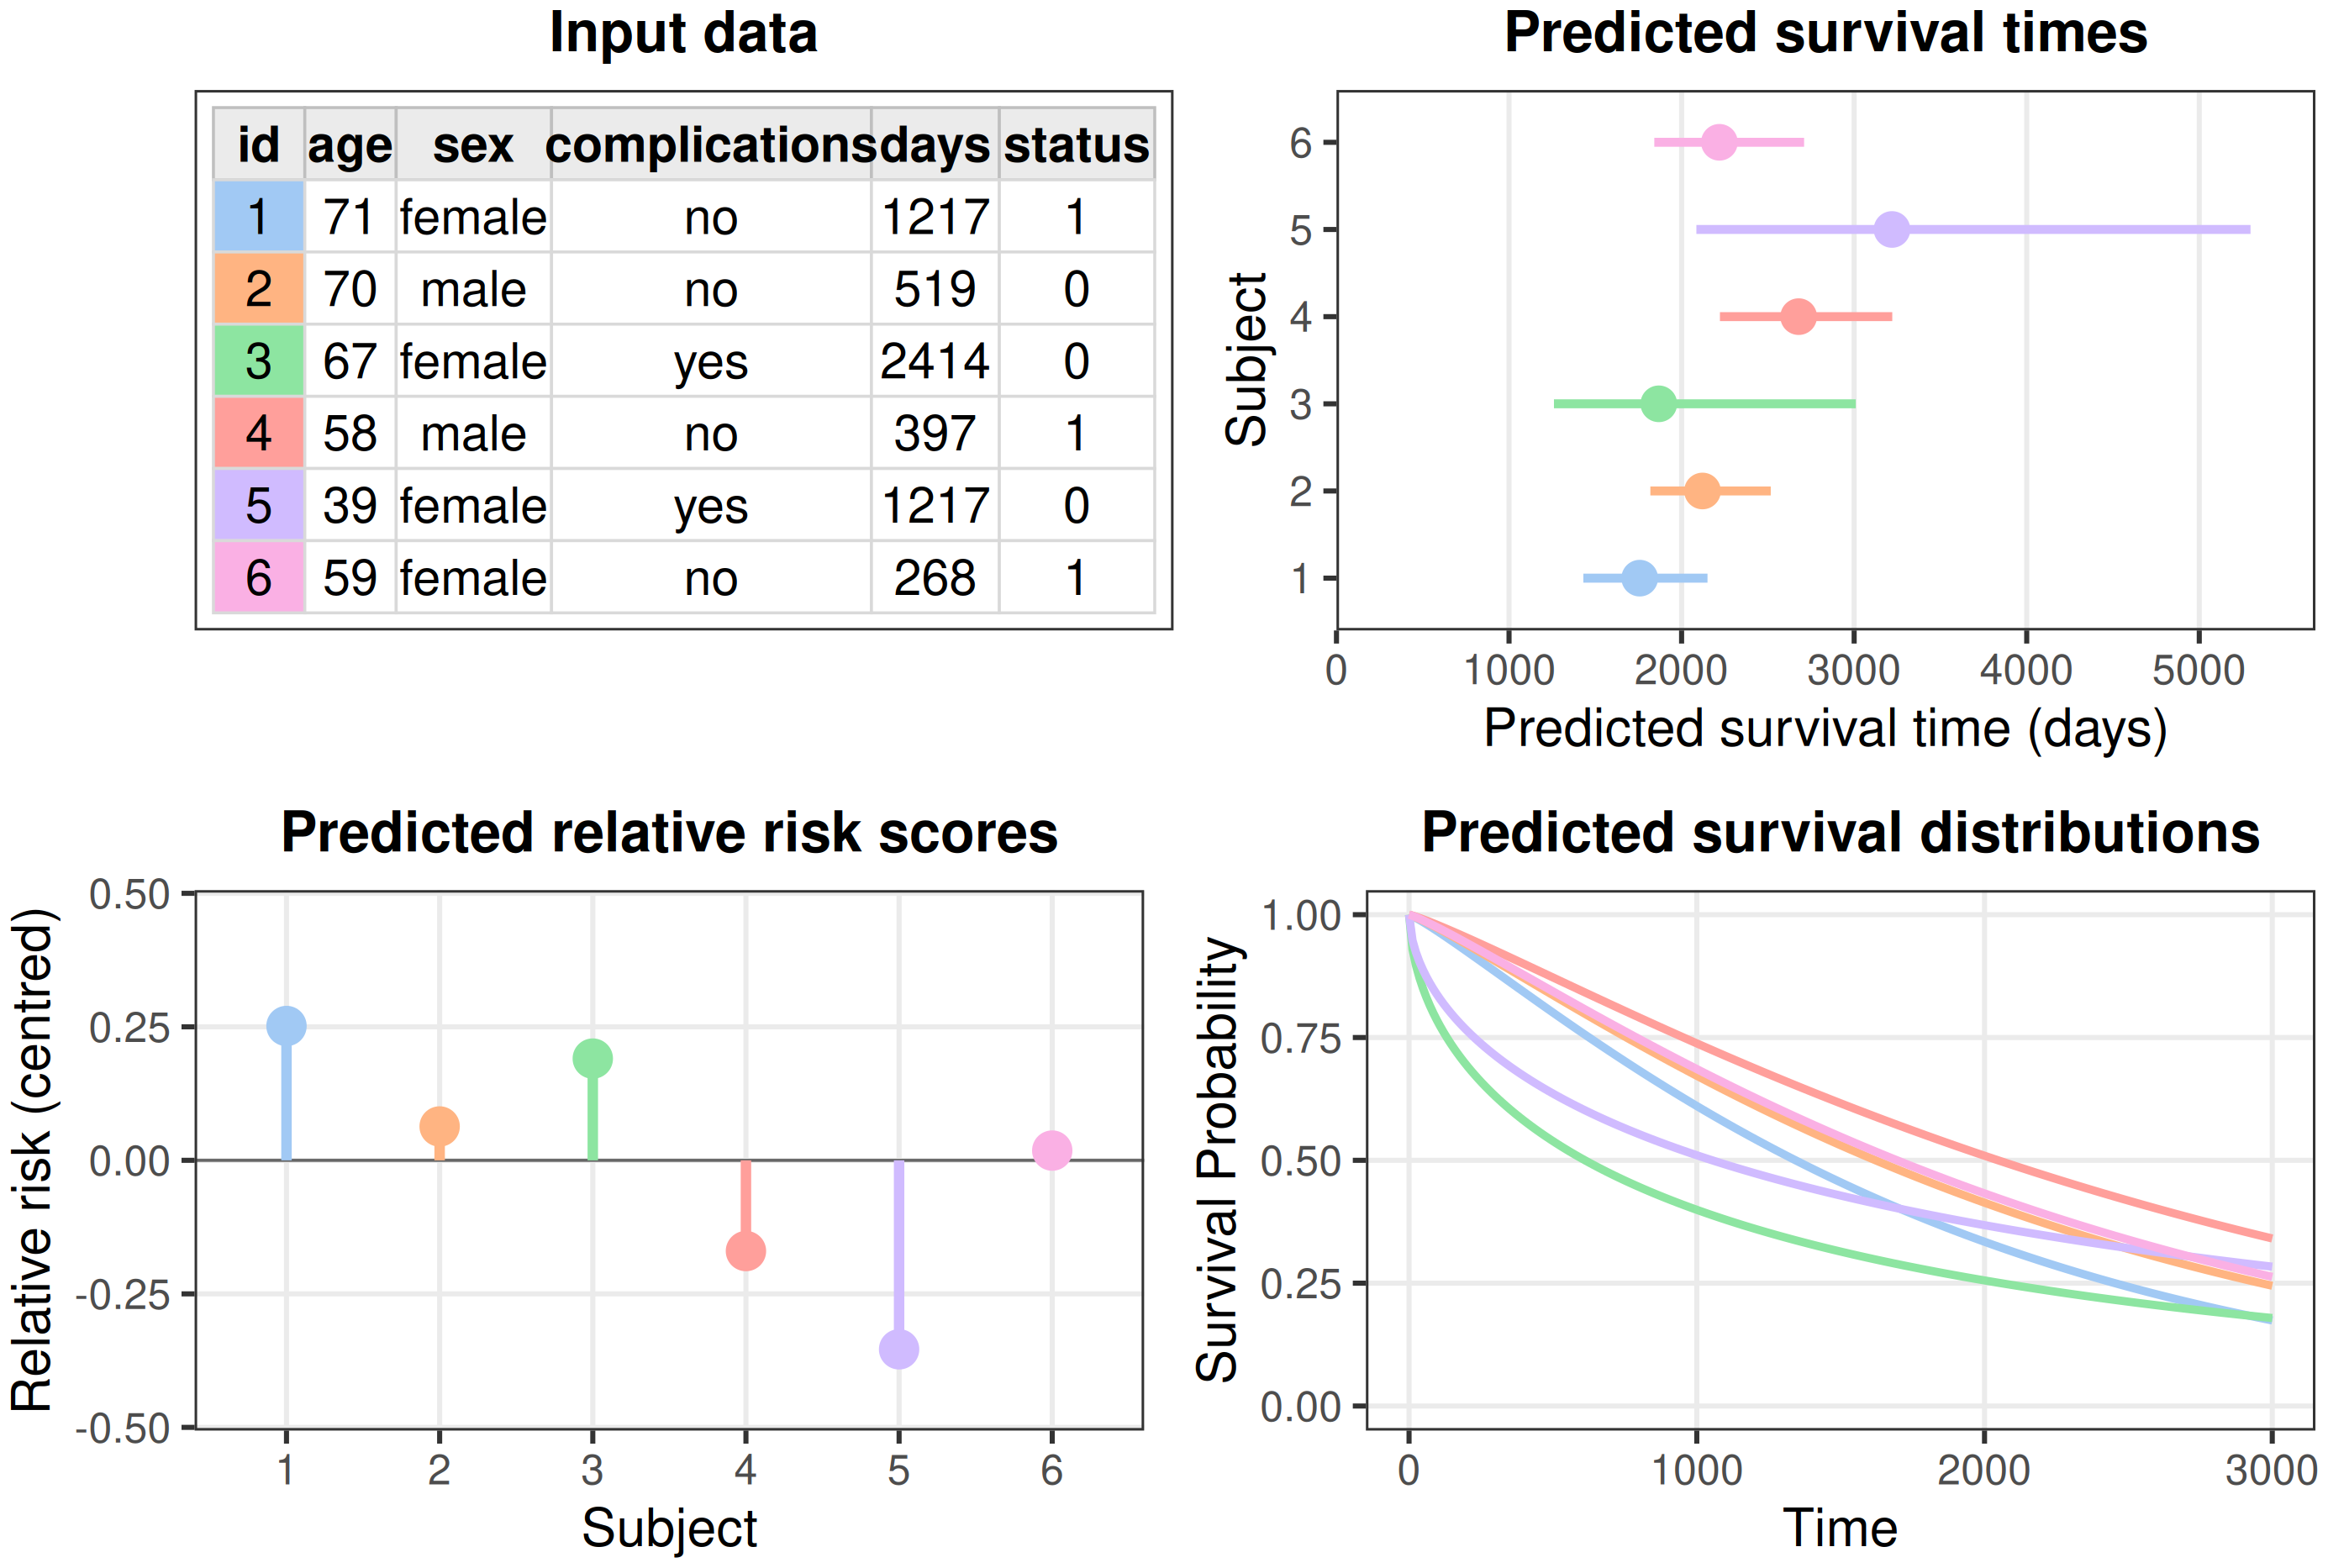
\includegraphics[width=1\linewidth,height=\textheight,keepaspectratio]{Figures/survtsk/fig-p1c6-predict-types.png}

}

\caption{\label{fig-p1c6-predict-types}Illustration of prediction types
using six patients from the \texttt{tumor} data set and a Weibull
accelerated failure time model. Tabular survival data (top-left) can be
used by an algorithm to make various prediction types, each conveying
different information. Survival times (top-right) provide a single
number estimating the time until an event takes place. Relative risk
scores (bottom-left) compare the risk of the event between subjects
within the same sample. Survival distributions (bottom-right) estimate
the probability of remaining event-free over time.}

\end{figure}%

\section{Predicting distributions}\label{sec-survtsk-dist}

Predicting a survival distribution\index{survival distribution} means
estimating the probability of an individual's event time over the
interval from time point \(0\) to \(\infty\). In principle, such
predictions are defined over the continuous non-negative real numbers,
\(\mathbb{R}_{\geq 0}\). In practice, the form of the prediction depends
on the modeling approach: parametric models typically define predictions
over continuous time, whereas several non- and semi-parametric
approaches represent predictions through discrete time points. Even when
predictions are continuous, they are often evaluated or visualized on a
discrete-time grid.

Theoretically, distributional prediction can target any of the
distribution-defining functions introduced in
Section~\ref{sec-distributions}, though predicting \(S(\tau)\) or
\(h(\tau)\) is most
common\index{survival function}\index{hazard function}. Mathematically,
the survival task associated with the distribution prediction type is
defined by \(g_S: \mathcal{X}\rightarrow \mathcal{S}\), where
\(\mathcal{S}\subseteq \operatorname{Distr}(\mathbb{R}_{\geq 0})\)
denotes a set of distributions on \(\mathbb{R}_{\geq 0}\). For competing
risks\index{competing risks}, distributional prediction usually returns
one cause-specific function per event type, so the number of prediction
functions is multiplied by the number of causes. More generally, in the
multi-state setting\index{multi-state models}, distributional prediction
generalizes to time-indexed transition probabilities between states,
represented as a transition probability matrix at each time point of
interest.

Communicating a predicted distribution over time can be a daunting task,
especially in settings such as healthcare with communication from a
clinician to patient. Instead, distribution predictions are commonly
used to derive time-specific survival probabilities, which represent the
probability of surviving beyond a relevant time point. For example, the
probability of being alive ten years after a diagnosis of Huntington's
disease. Predicting `\(\tau\)-year survival
probabilities'\index{t-year survival probability@$\tau$-year survival probability}
is sometimes mistakenly framed as a classification problem, in which a
model predicts whether an event will occur by a fixed time. This is
misleading as traditional classification models cannot incorporate
observations censored before the time horizon of interest, and
discarding such observations would bias any results (Loh et al. 2025).
See Chapter~\ref{sec-ipcw-reduction} for the appropriate use of
classification models in this context.

Survival distributions can also be used for decision making by
establishing thresholds on survival probabilities. For example, in an
engineering context, a survival model might be used to estimate the
reliability of a jet engine over time, with a maintenance rule defined
such that the engine is serviced once the predicted survival probability
falls below a predefined reliability threshold (which could be as high
as 0.95).

Another source of potential confusion can arise when interpreting
survival distribution predictions in the single-event setting. In
reality, an event either occurs or does not occur at a particular time,
making it natural to question what an individual's predicted survival
distribution actually represents. Figure~\ref{fig-p1c6-heavisides}
illustrates the goal of survival distribution
prediction.\index{Heaviside function} The top-left panel shows the
idealized `real-world' survival trajectories for multiple individuals,
each represented by a Heaviside step function that drops from \(1\) to
\(0\) at the event time. The top-right panel highlights one such
individual trajectory. The bottom-left panel shows the objective of
survival distribution prediction: a smooth survival function summarizing
the average behavior of these individual event trajectories across a
population. Finally, the bottom-right panel shows the same events
stratified by a binary covariate, producing one survival distribution
for each subgroup. In machine learning, this idea is generalized by
conditioning on the full covariate vector, potentially yielding a
different predicted survival distribution per individual. Hence, an
individual's predicted survival distribution can be interpreted as the
average survival experience among a large group of individuals sharing
the same covariate profile.

\begin{figure}

\centering{

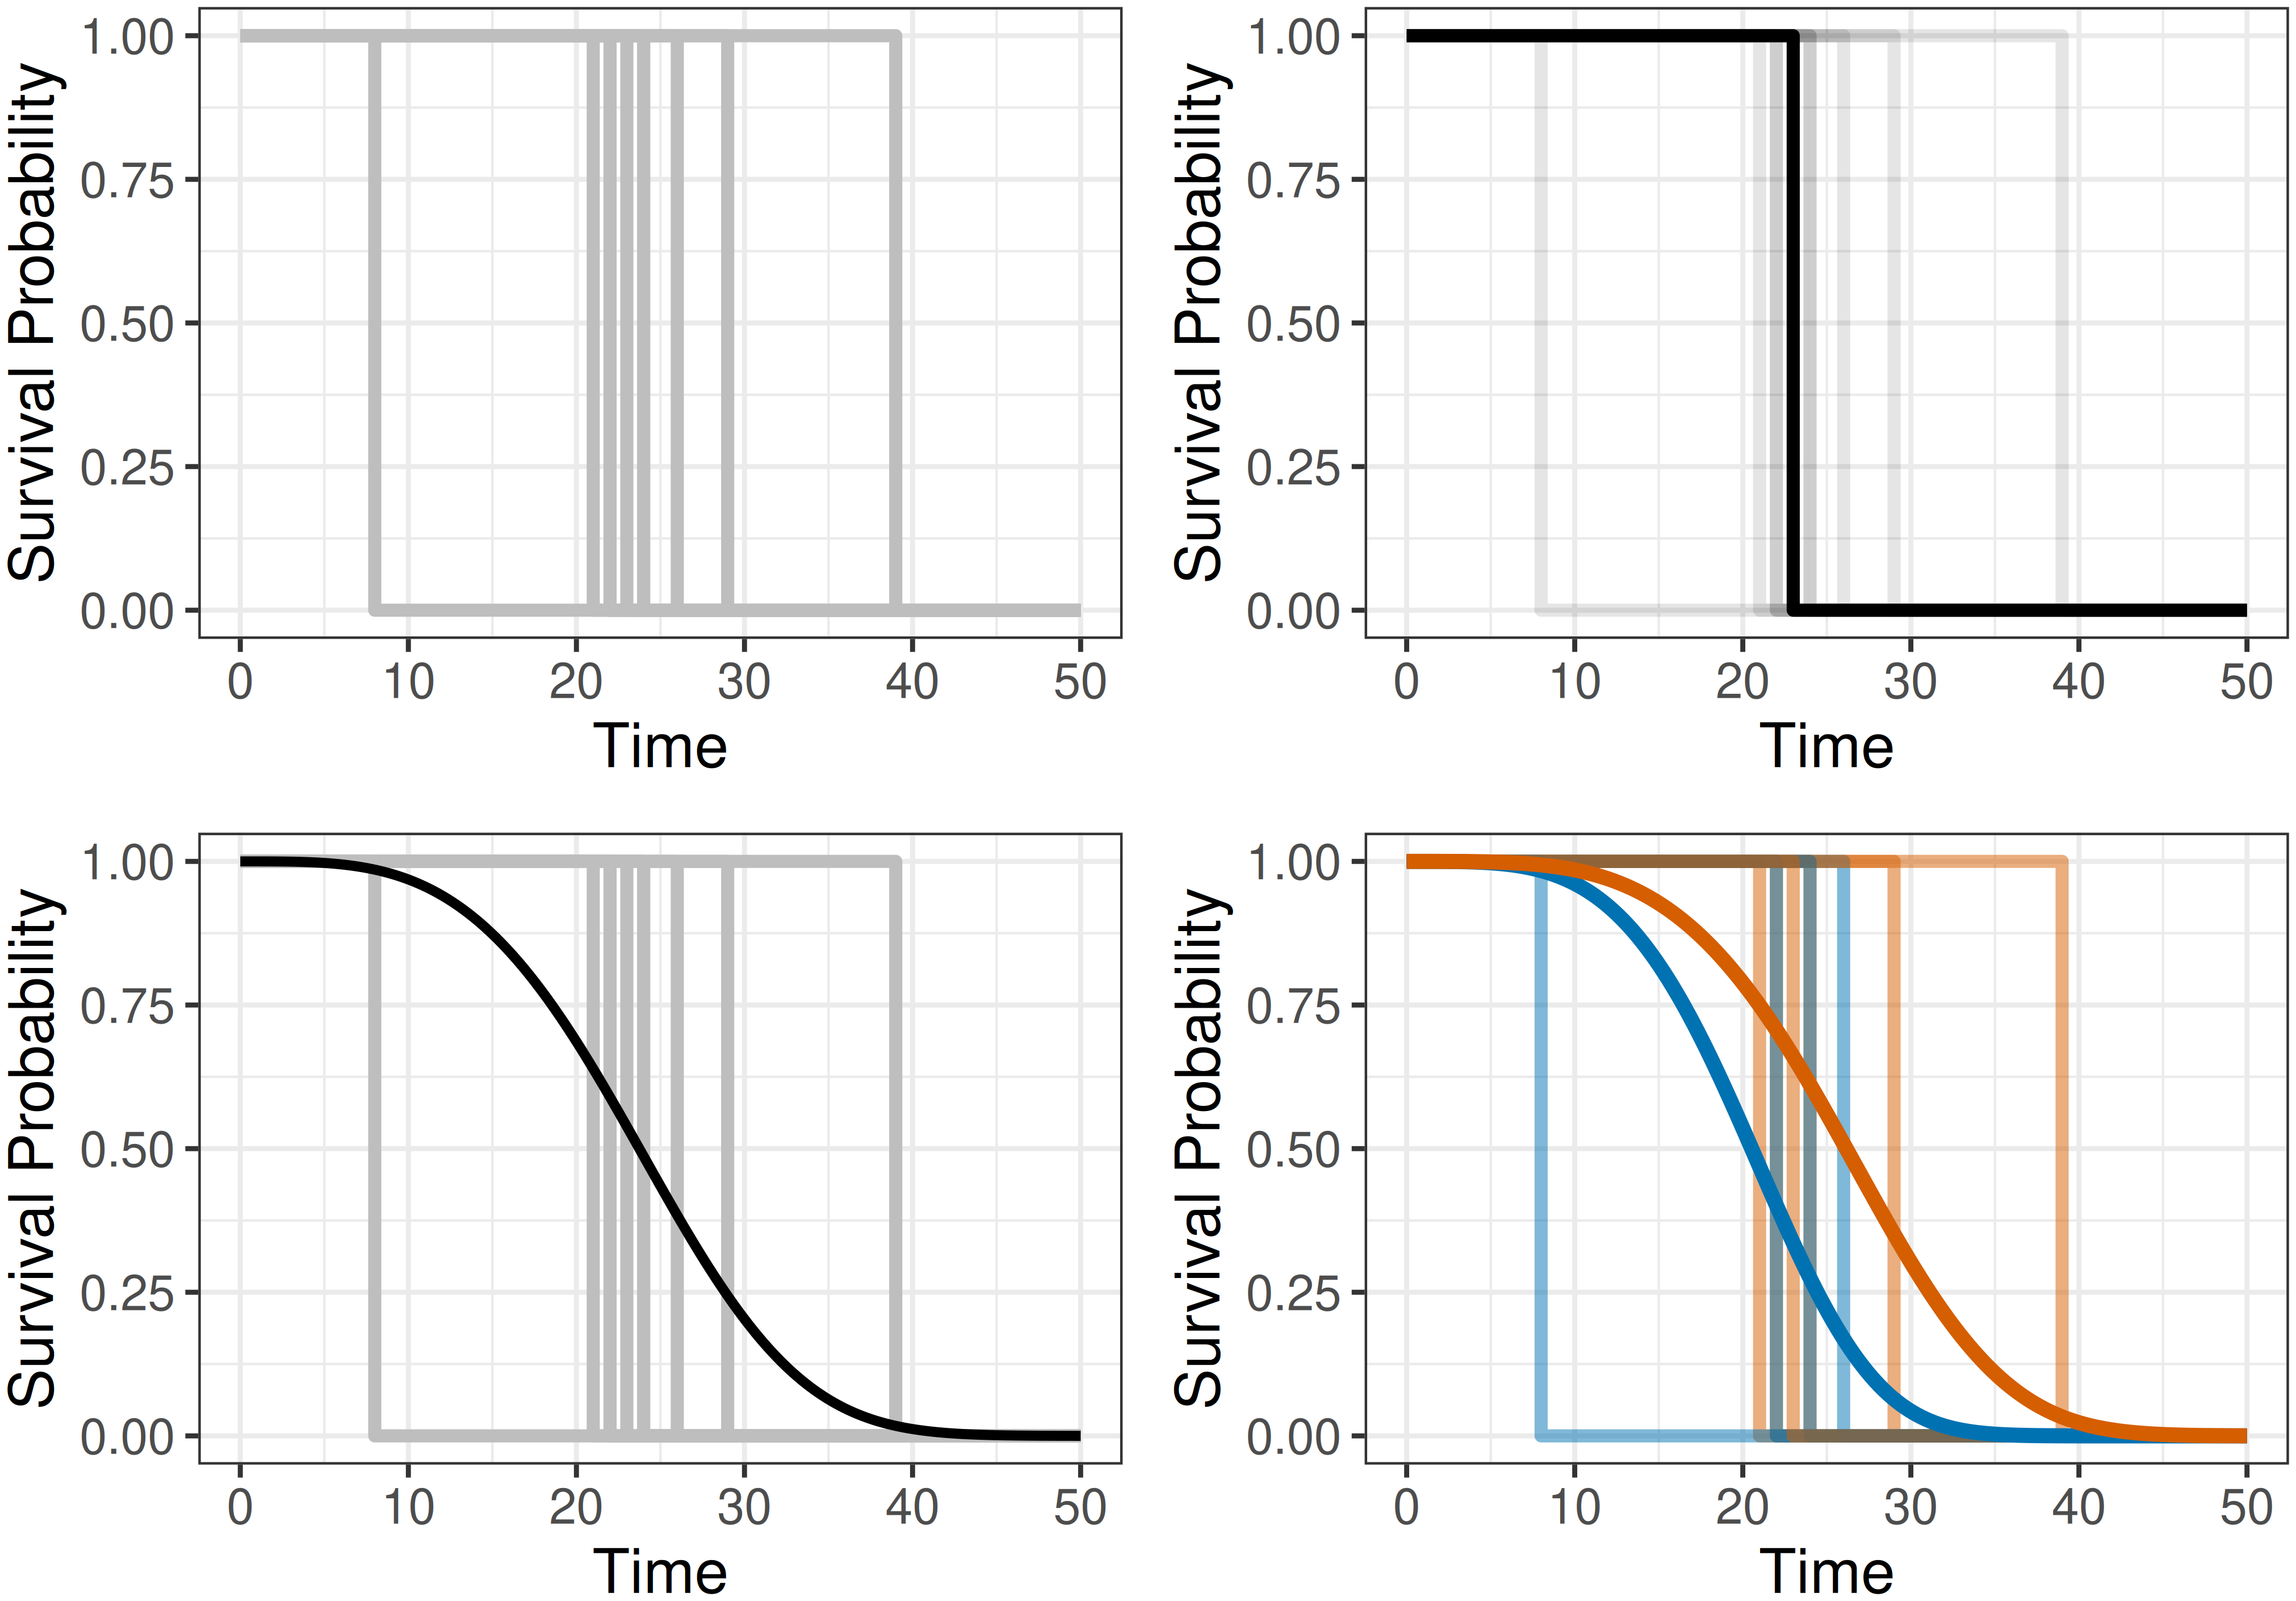
\includegraphics[width=1\linewidth,height=\textheight,keepaspectratio]{Figures/survtsk/fig-p1c6-heavisides.png}

}

\caption{\label{fig-p1c6-heavisides}Demonstrating the relationship from
theoretical real-world event curves to survival distribution
predictions.}

\end{figure}%

\section{Predicting relative risks}\label{sec-survtsk-risk}

Predicting relative risk\index{relative risk} scores refers to
estimating a value that ranks individuals in a cohort according to their
predicted risk of experiencing the event. These scores are meaningful
only in comparison to other individuals evaluated on the same scale;
they cannot be interpreted in isolation, nor can they be compared to
scores produced by a different model, except under very strong
assumptions. The interpretation of these scores can also differ across
model classes, parameterizations, and even software implementations. For
example, some models produce scores where larger values correspond to
higher risk, whereas others produce scores where smaller values
correspond to higher risk. To avoid ambiguity, throughout this book
larger values always correspond to higher risk and smaller values
correspond to lower risk. In machine learning terms, the relative risk
prediction task\index{machine learning task} is the problem of
estimating \(g_S: \mathcal{X}\rightarrow \mathbb{R}\).

As an example of this prediction type, consider three individuals,
\(\{i,j,k\}\) with predicted risks \(\{0.5, 10, 0.1\}\), respectively.
From these values, two broad types of conclusion can be drawn.

\begin{enumerate}
\def\labelenumi{\arabic{enumi}.}
\tightlist
\item
  Conclusions comparing individuals:
\end{enumerate}

\begin{itemize}
\tightlist
\item
  The corresponding ranks for \(\{i,j,k\}\) are \(\{2,3,1\}\).
\item
  \(k\) has the lowest risk and \(j\) the highest risk.
\item
  The risk of \(i\) is slightly higher than that of \(k\), whereas
  \(j\)'s risk is substantially higher than both.
\end{itemize}

\begin{enumerate}
\def\labelenumi{\arabic{enumi}.}
\setcounter{enumi}{1}
\tightlist
\item
  Conclusions comparing risk groups:
\end{enumerate}

\begin{itemize}
\tightlist
\item
  Thresholding at \(0.4\) classifies \(k\) as low-risk and \(i\) and
  \(j\) as high-risk.
\item
  Thresholding at \(1.0\) classifies \(i\) and \(k\) as low-risk and
  \(j\) as high-risk.
\end{itemize}

As in other domains, differences in relative risks should always be
interpreted cautiously. In the example above, \(j\)'s relative risk is
\(100\) times that of \(k\); however, if \(k\)'s absolute probability of
experiencing the event is \(0.0001\), then \(j\)'s absolute probability
remains small at \(0.01\).

Estimation and interpretation of risks in the competing risks setting
follows similar principles. However, one must take care to clearly
identify if the task of interest is to predict risks for each of the
\(q\) causes, \(g_S: \mathcal{X}\rightarrow \mathbb{R}^q\), or a single
all-cause risk\index{all-cause risk}. In multi-state
models\index{multi-state models}, the notion of a single scalar `risk'
is less clearly defined and any risk-based summaries should be
interpreted with caution.

\subsection{Distributions and risks}\label{distributions-and-risks}

In general, it is not possible to uniquely recover a survival
distribution from a relative risk score\index{survival distribution},
except in very specific cases (discussed in
Section~\ref{sec-survtsk-PI}). The reverse direction, deriving a risk
score from a predicted survival distribution, is more common. One stable
approach to compute a risk score is by summing the estimated cumulative
hazard, which provides a measure of expected mortality for individuals
with similar covariate profiles (Ishwaran et al.
2008)\index{expected mortality} (see Section~\ref{sec-rsf-risks} for
intuition from random survival forests and Section~\ref{sec-alpha} for a
related calibration measure). The \emph{expected mortality} for an
individual \(i\) is defined as,

\[
\sum_{\tau \in \mathcal{T}} -\log(\hat{S}(\tau \mid \mathbf{x}_i)) = \sum_{\tau \in \mathcal{T}} \hat{H}(\tau \mid \mathbf{x}_i),
\]

where \(\hat{S}(\cdot \mid \mathbf{x}_i)\) is the predicted survival
function, \(\hat{H}(\cdot \mid \mathbf{x}_i)\) is the corresponding
cumulative hazard, and \(\mathcal{T}\) is the set of observed time
points. Larger values indicate greater expected mortality and thus a
higher risk profile. As a concrete example, consider two individuals,
\(i\) and \(j\), with predicted survival probabilities at times
\(\mathcal{T}= \{0,1,2,3\}\):

\[
\begin{aligned}
&(\tau, \hat{S}(\tau \mid \mathbf{x}_i)) = (0, 1), (1, 0.8), (2, 0.4), (3, 0.15), \\
&(\tau, \hat{S}(\tau \mid \mathbf{x}_j)) = (0, 1), (1, 0.6), (2, 0.4), (3, 0.35).
\end{aligned}
\]

From these values alone, it is not immediately obvious which individual
would be considered at higher risk. The corresponding cumulative hazards
are,

\[
\begin{aligned}
&(\tau, \hat{H}(\tau \mid \mathbf{x}_i)) = (0, 0), (1, 0.22), (2, 0.92), (3, 1.90), \\
&(\tau, \hat{H}(\tau \mid \mathbf{x}_j)) = (0, 0), (1, 0.51), (2, 0.92), (3, 1.05).
\end{aligned}
\]

Using the expected mortality approach yields relative risk scores of

\[
\begin{aligned}
&\sum_{\tau \in \mathcal{T}} \hat{H}(\tau \mid \mathbf{x}_i) = 0 + 0.22 + 0.92 + 1.90 = 3.01, \\
&\sum_{\tau \in \mathcal{T}} \hat{H}(\tau \mid \mathbf{x}_j) = 0 + 0.51 + 0.92 + 1.05 = 2.48.
\end{aligned}
\]

Under this method, the risk score of \(i\) is approximately \(1.2\)
times higher than that of individual \(j\).

\section{Predicting survival times}\label{sec-survtsk-time}

Predicting a survival time\index{survival time} refers to estimating
when an individual will experience the event of interest.
Mathematically, this corresponds to estimating
\(g_S: \mathcal{X}\rightarrow \mathbb{R}_{>0}\), that is, predicting a
single positive value on \((0,\infty)\).

Survival time predictions may initially appear attractive as they seem
intuitive and easy to interpret. However, evaluating survival time
predictions is practically very challenging and as such reliance on
these predictions is ill-advised. To illustrate this, consider an
individual censored at time \(\tau=5\). There is no way to know if the
event would have occurred at \(\tau=6\) or \(\tau=600\); all that can be
known is that the event did not occur before \(\tau=5\). As a result, it
is impossible to assess how close a time prediction is to the true,
unobserved event time. Even when a prediction is clearly incorrect, the
magnitude of its error cannot be quantified. For the same individual
censored at \(\tau=5\), suppose a model predicts a survival time of
\(\hat{t}=3\). This prediction is clearly wrong as the event did not
occur before \(\tau=5\). However, the prediction might only be slightly
wrong if the true event time were \(\tau=6\), or extremely wrong if the
true event time were \(\tau=600\).

The challenge of censoring is particularly complex for evaluating
survival time predictions, which reduce the prediction to a single
scalar quantity. By contrast, probabilistic predictions make use of the
survival process over time and can thus enable meaningful evaluation
before the outcome time (for example, with the scoring rules in
Chapter~\ref{sec-rules}), while risk-based predictions are relative and
can exploit comparative information such as pairwise ordering (for
example, with the discrimination measures in
Chapter~\ref{sec-eval-crank}). For these reasons, this book recommends
predicting and evaluating survival distributions and only then deriving
time-oriented summaries.

Event history analysis\index{event history analysis} faces similar
challenges due to the presence of censoring. The term `survival time' is
also ill-defined unless the event or transition of interest is
explicitly specified, as it may refer either to the time until a
particular event or transition or, more generally, to the time until any
event occurs. In multi-state models\index{multi-state models}, one
possible alternative is to estimate sojourn times\index{sojourn times},
which represent the expected time spent in a given state and can be
derived from estimated transition
probabilities\index{transition probability}. Sojourn times are
particularly well defined in Markov\index{Markov} and semi-Markov
models, where they arise naturally from stochastic process theory (Ibe
2013). However, although sojourn times may be estimable, censoring still
makes their evaluation challenging.

\subsection{Times and risks}\label{times-and-risks}

Converting a survival time prediction to a risk prediction is
conceptually straightforward, as survival times encode natural ordering.
An individual predicted to survive longer is, by definition, at lower
overall risk\index{relative risk}. Formally, if \(\hat{t}_i,\hat{t}_j\)
denote predicted survival times and \(\hat{r}_i,\hat{r}_j\) are
associated rankings, then

\[
\hat{t}_i > \hat{t}_j \Rightarrow \hat{r}_i < \hat{r}_j.
\]

The reverse transformation, from ranking to survival time, is generally
not possible without strong assumptions as relative risk scores are
usually abstract quantities that do not map directly to meaningful
survival times.

\subsection{Times and distributions}\label{times-and-distributions}

Moving from a survival time to a distribution
prediction\index{survival distribution} is uncommon. Given the
availability of models that directly predict survival distributions, and
the difficulty of evaluating survival time predictions, there is little
motivation for this transformation. It is nonetheless \emph{possible},
as in regression settings, to construct a distribution around a central
estimate \(\hat{t}\) by assuming a parametric form. For example, one
could use a truncated normal distribution on \(\mathbb{R}_{\geq 0}\)
with location \(\hat{t}\) and standard deviation \(\sigma\), where
\(\sigma\) is assumed or estimated. Such constructions depend on strong
distributional assumptions and are rarely used in practice.

It is more common to reduce a prediction from a probability distribution
to a survival time by attempting to compute the mean or median of the
distribution. For a non-negative event time, the expected survival time
can be computed from the survival function using the `Darth Vader
rule'\index{Darth Vader rule} (Muldowney, Ostaszewski, and Wojdowski
2012),

\begin{equation}\phantomsection\label{eq-darth}{
\mathbb{E}[Y] = \int^\infty_0 S_Y(y) \ \,\mathrm{d}y.
}\end{equation}

However, (\ref{eq-darth}) requires distributions to be
proper\index{proper distribution} but as discussed in
Section~\ref{sec-distributions-continuous}, this is often not the case
for estimated survival distributions, especially those that depend on
non-parametric estimators (Section~\ref{sec-surv-estimation-non-param}).
Heuristics have been proposed to address this issue, including linear
extrapolation of the survival curve to zero, or an immediate drop to
zero at the final time point. However, these can introduce bias into
estimated survival times (Han and Jung 2022; Sonabend, Bender, and
Vollmer 2022).

The survival time could also be reported as the median survival
time\index{median survival time}, defined as the earliest time at which
the predicted survival probability drops to \(0.5\),

\[
\hat{t}_{50} = \inf\{\tau: \hat{S}(\tau) \leq 0.5 \}.
\]

However, this quantity is only defined if the estimated survival curve
reaches \(0.5\) within the observed follow-up period, which is never
guaranteed.

An alternative is to summarize the predicted distribution with the
\emph{restricted mean survival time}
(RMST)\index{restricted mean survival time} (Andersen, Hansen, and Klein
2004; Han and Jung 2022). Rather than integrating over the entire time
axis as in (\ref{eq-darth}), the RMST truncates the integral at a finite
horizon:

\[
\operatorname{RMST}(\tau) = \int^\tau_0 S_Y(y) \,\mathrm{d}y.
\]

It follows from (\ref{eq-darth}) that
\(\operatorname{RMST}(\infty) = \mathbb{E}[Y]\). Whereas
(\ref{eq-darth}) represents the average survival time over
\([0,\infty)\), the RMST represents the average survival time up to
\(\tau\),

\begin{equation}\phantomsection\label{eq-rmst-min}{
\operatorname{RMST}(\tau) = \mathbb{E}[\min(Y, \tau)],
}\end{equation}

which treats all events occurring after \(\tau\) as if they occurred at
\(\tau\). The RMST is well-defined even when the predicted distribution
is improper\index{improper distribution}, provided that the survival
function is defined up to \(\tau\); in practice, \(\tau\) is usually
chosen within the range of observed follow-up times.

Say individuals are observed over a six-year time period and
administrative censoring\index{censoring!type I} is present so that
\(\mathbb{E}[Y]\) cannot be reliably computed. One \emph{can} compute
\(\operatorname{RMST}(6)\) to provide an interpretable truncated summary
such that when the mean survival time exists,\index{mean survival time}
\(\operatorname{RMST}(6) \leq \mathbb{E}[Y]\). This results in a
meaningful statement such as: ``the average survival time is at least
\(\operatorname{RMST}(6)\)'', or ``over a six-year horizon, the
restricted mean survival time is \(\operatorname{RMST}(6)\)''
(Figure~\ref{fig-p1c6-rmst}).

The RMST is commonly used to summarize the effect of covariates,
particularly treatments in a healthcare setting. For example, suppose a
researcher is interested in understanding how a treatment affects
three-year and six-year survival for a given disease. Assume the
predicted survival curves for the treated group \(i\) and untreated
group \(j\) are

\[
\begin{aligned}
(\tau, \hat{S}(\tau \mid \mathbf{x}_i)) = (0, 1.00), (1, 0.80), (2, 0.75), (3, 0.75), (4, 0.70), (5, 0.60), \\
(\tau, \hat{S}(\tau \mid \mathbf{x}_j)) = (0, 1.00), (1, 0.90), (2, 0.85), (3, 0.60), (4, 0.50), (5, 0.10). \\
\end{aligned}
\]

The corresponding RMSTs at \(\tau=3\) and \(\tau=6\) are, using a
left-endpoint Riemann sum approximation (so the value at \(\tau=5\) is
used for the interval \([5,6)\)) with unit intervals,

\[
\begin{aligned}
\operatorname{RMST}_i(3) &\approx 1.00 + 0.80 + 0.75 = 2.55, \\
\operatorname{RMST}_j(3) &\approx 1.00 + 0.90 + 0.85 = 2.75, \\
\operatorname{RMST}_i(6) &\approx 1.00 + 0.80 + 0.75 + 0.75 + 0.70 + 0.60 = 4.60, \\
\operatorname{RMST}_j(6) &\approx 1.00 + 0.90 + 0.85 + 0.60 + 0.50 + 0.10 = 3.95. \\
\end{aligned}
\]

Over the three-year follow-up period, group \(j\) is expected to remain
event-free for approximately \(0.20\) years (\(2.4\) months) longer than
group \(i\). In contrast, over the six-year interval, group \(i\) is
expected to remain event-free for approximately \(0.65\) years (\(7.8\)
months) longer than group \(j\). Computing the RMST at these two
horizons provides interpretable summaries: the treatment may offer no
short-term benefit within three years, and may even be associated with
short-term harm, but confers a meaningful advantage over a longer
six-year horizon.

These results, visualized in Figure~\ref{fig-p1c6-rmst}, illustrate a
key feature of the RMST. By fixing the time horizon \(\tau\), the
contribution of survival differences after \(\tau\) is ignored. As the
RMST at \(\tau=6\) only summarizes the survival curve up to six years,
survival differences after this point do not affect the summary. Even if
members of group \(i\) were to survive many years longer than members of
group \(j\), the RMST at \(\tau=6\) treats all event times after six
years as if they occurred at that time, a consequence of
(\ref{eq-rmst-min}). As a result, the RMST difference over the six-year
horizon remains modest, even though the long-term survival difference,
if it were estimable, could be substantial.

\begin{figure}

\centering{

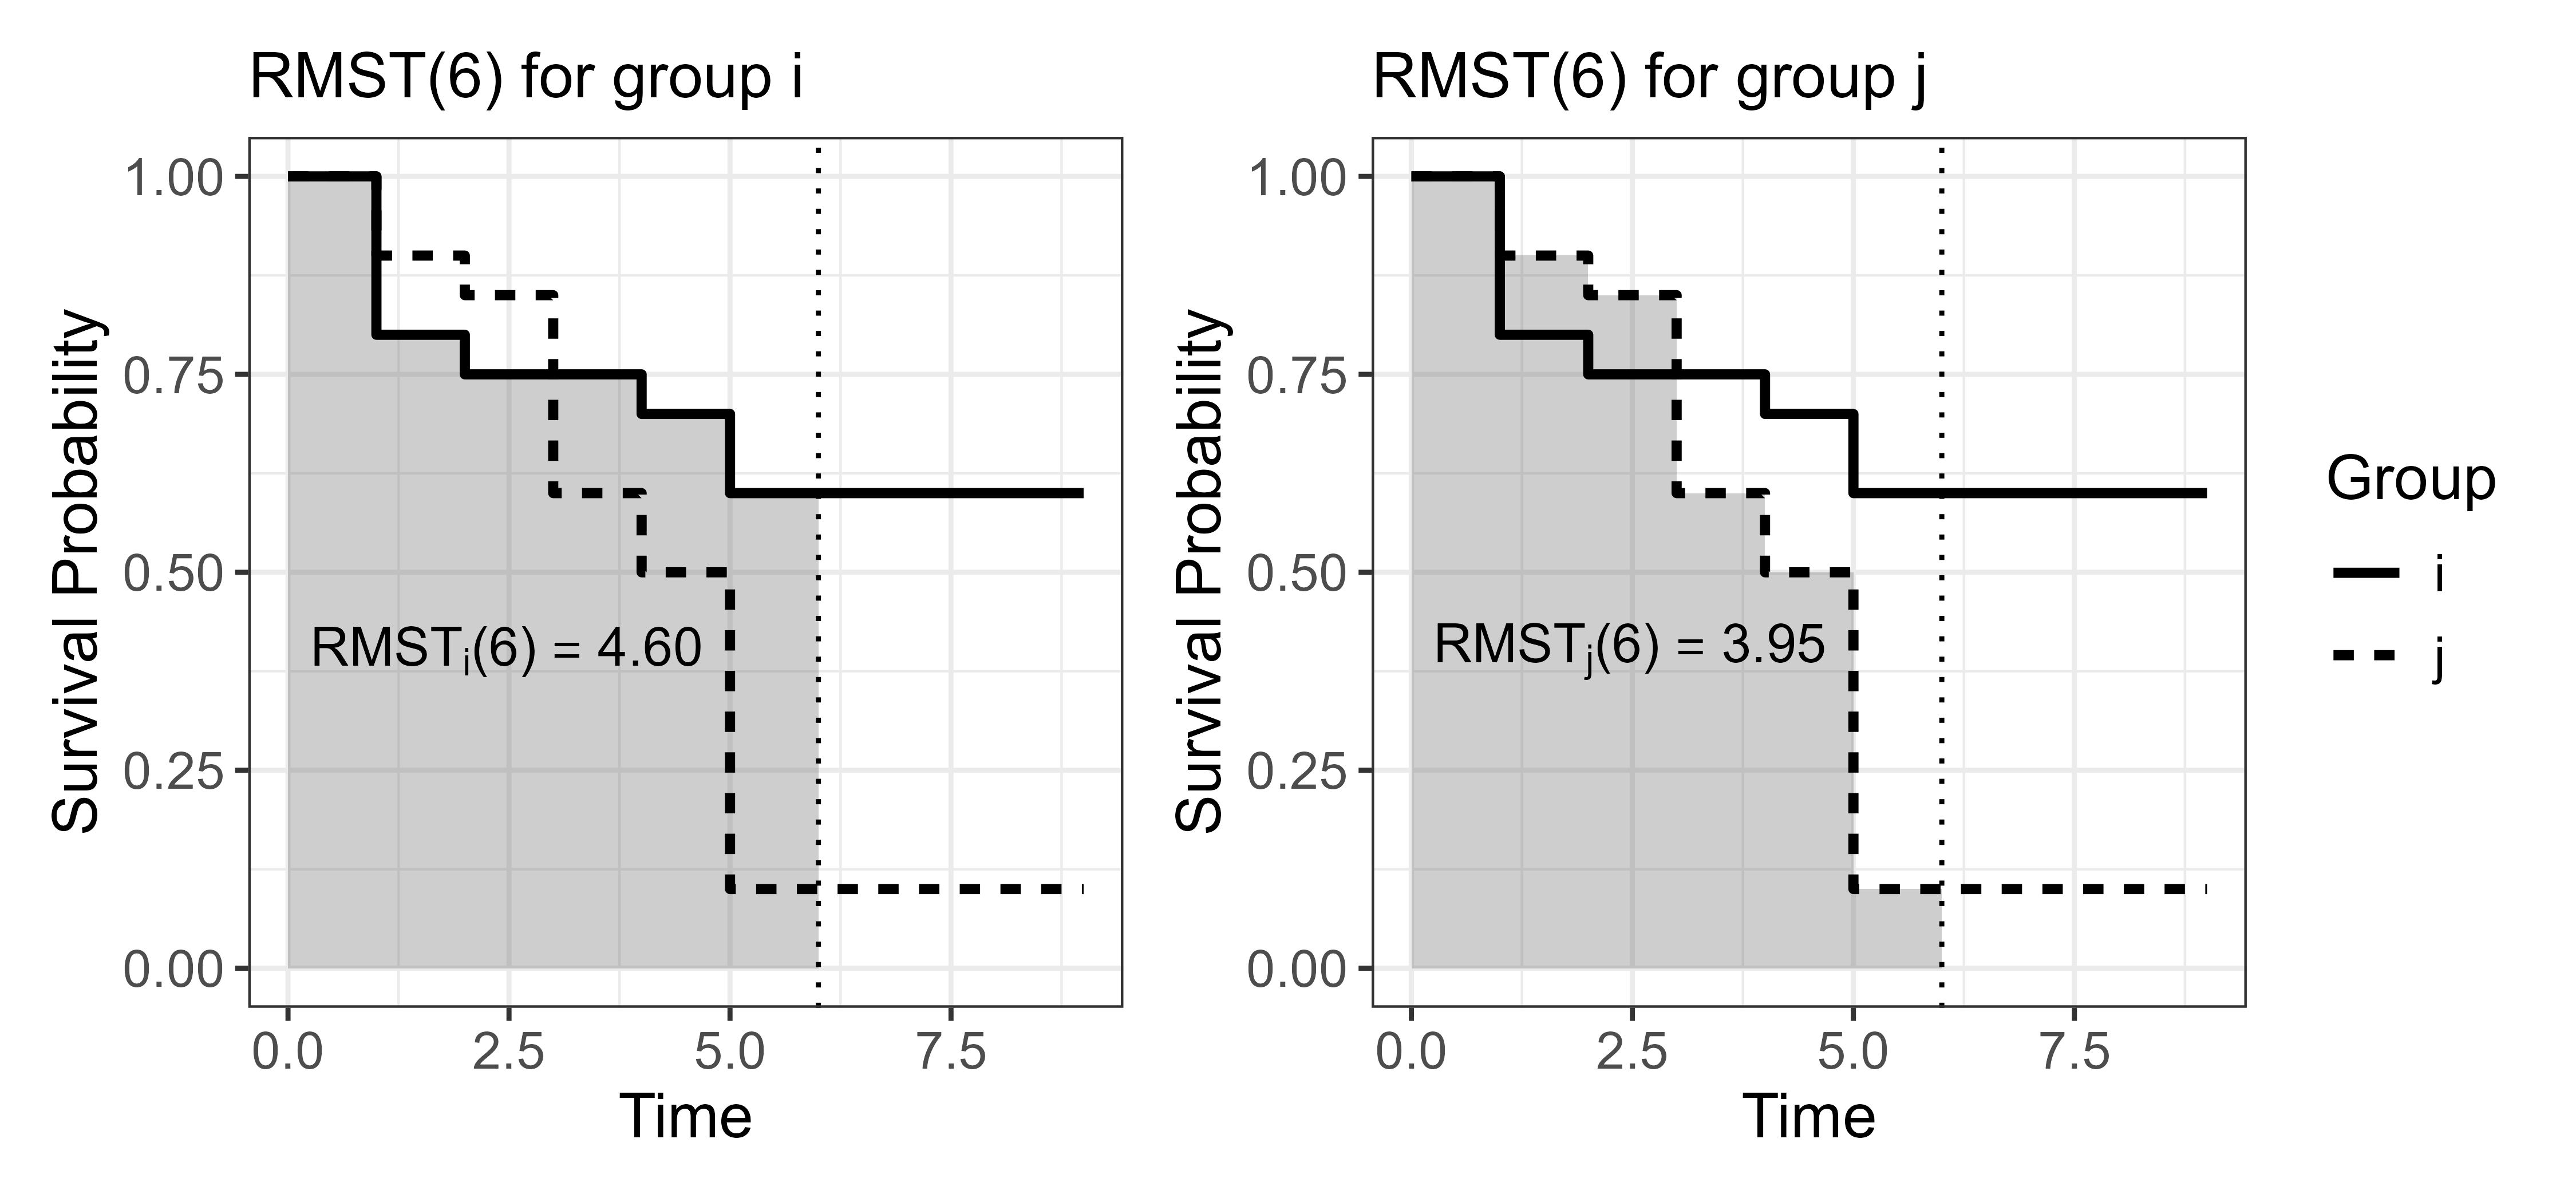
\includegraphics[width=1\linewidth,height=\textheight,keepaspectratio]{Figures/survtsk/fig-p1c6-rmst.png}

}

\caption{\label{fig-p1c6-rmst}Illustrating the RMST at \(\tau=6\). The
RMST is the area under the survival curve up to the time horizon. The
shaded rectangles show a left-endpoint Riemann sum approximation, so the
value at time \(5\) contributes over the interval from \(5\) to \(6\).
The solid line shows the survival curve for group \(i\) and the dashed
line for group \(j\). The left panel shows the RMST at \(\tau=6\) for
group \(i\) and the right panel for group \(j\). The figure illustrates
that RMST depends only on the area under the survival curve up to the
chosen time horizon, so tail behavior after that horizon is ignored.}

\end{figure}%

\section{Prognostic index predictions}\label{sec-survtsk-PI}

In medical terminology, a \emph{prognostic
index}\index{prognostic index} is a quantity that summarizes an
individual's risk of experiencing the event of interest based on
observed risk factors. A prognostic index is closely related to a
relative risk score (Section~\ref{sec-survtsk-risk}), but the two terms
emphasize different aspects of the prediction. A relative risk score is
any scalar prediction whose ordering reflects relative risk. A
prognostic index \emph{additionally} emphasizes an interpretable
model-specific mapping from covariates to that scalar prediction.

Formally, a prognostic index is:

\[
\hat{r}_i = \psi(\hat{g}(\mathbf{x}_i)),
\]

where \(\hat{g}\) is a scalar prediction (such as a relative risk), and
\(\psi\) is a transformation chosen so that the resulting quantity has
the desired scale, sign, and interpretation. In later chapters, \(\psi\)
is specifically referred to as a \emph{response
function}\index{response function}. For simple linear models, the
prognostic index is a transformation of the \emph{linear
predictor}\index{linear predictor},
\(\eta_i := \mathbf{x}_i^\top\boldsymbol{\beta}\) where
\(\mathbf{x}_i \in \mathbb{R}^p\) are covariates and
\(\boldsymbol{\beta}\in \mathbb{R}^p\) are model coefficients. For more
flexible models, \(\hat{g}\) may be non-linear.

A prognostic index can serve several purposes, including:

\begin{enumerate}
\def\labelenumi{\arabic{enumi}.}
\tightlist
\item
  Scaling and/or normalization: for example, to improve interpretability
  and visualization;
\item
  Ensuring meaningful results: for example,
  \(\psi(\boldsymbol{\eta}) = \exp(\boldsymbol{\eta})\) transforms
  covariates to act multiplicatively on the resulting prognostic score,
  which is appropriate for models in which the covariates rescale the
  underlying risk instead of inducing additive shifts (explored further
  in Section~\ref{sec-classical-cox});
\item
  Interpretability conventions: for example,
  \(\psi(\boldsymbol{\eta}) = -\boldsymbol{\eta}\) might be sufficient
  to ensure that larger values correspond to higher risk.
\end{enumerate}

In event history analysis, prognostic indices can be defined
analogously, although their precise form depends on the setting and
prediction target, for example, whether interest lies in
transition-specific, cause-specific, or all-cause risk.

\subsection{Prognostic index, risks, and
times}\label{prognostic-index-risks-and-times}

A prognostic index is naturally interpreted as a relative risk
score\index{relative risk}. When used in this way, it is essential that
both the magnitude and sign of the index align with the convention
adopted above, meaning that larger values must correspond to a higher
risk of experiencing the event.

The reverse transformation, from risk score to prognostic index, does
not hold in general. For example, models introduced in
Chapter~\ref{sec-svm} and Chapter~\ref{sec-boost} directly predict risk
scores that are useful for ranking individuals but do not necessarily
have an immediate covariate-level
interpretation\index{gradient boosting machines}\index{support vector machines}.
Therefore, reporting a prognostic index emphasizes that the predicted
quantity is interpretable in its own right, much like a survival time
prediction\index{survival time}.

There is no direct mapping between a prognostic index and survival time.
However, a prognostic index may be used to construct a distribution
prediction (discussed next), from which a time-based summary can be
derived.

\subsection{Prognostic index and
distributions}\label{prognostic-index-and-distributions}

In general, a prognostic index cannot be uniquely recovered from a
predicted survival distribution\index{survival distribution} without
additional modeling assumptions. By contrast, constructing a survival
distribution conditional on a prognostic index is common in survival
analysis. Many survival models predict survival distributions by first
estimating a group-wise survival distribution, often using
non-parametric estimators\index{non-parametric estimator}
(Section~\ref{sec-surv-estimation-non-param}), then combine this
estimate with an individual's prognostic index. The manner in which
these components are combined is algorithm-specific and discussed in
detail in Part III.

As a concrete illustration, one class of models known as `proportional
hazards models'\index{proportional hazards} (described in full in
Section~\ref{sec-classical-cox}), construct survival predictions of the
form

\[
S_{PH}(\tau \mid \mathbf{x}_i)= S_0(\tau)^{\exp(\hat{g}(\mathbf{x}_i))},
\]

where \(S_0(\tau)\) is known as the baseline survival
function\index{baseline survival function}, \(\hat{g}(\mathbf{x}_i)\) is
the model prediction, and \(\exp(\hat{g}(\mathbf{x}_i))\) serves as a
prognostic index\index{prognostic index}.

\section{Conclusion}\label{conclusion-3}

\begin{tcolorbox}[enhanced jigsaw, toprule=.15mm, bottomtitle=1mm, opacityback=0, breakable, leftrule=.75mm, title={Key takeaways}, toptitle=1mm, bottomrule=.15mm, colback=white, colframe=quarto-callout-warning-color-frame, titlerule=0mm, opacitybacktitle=0.6, coltitle=black, rightrule=.15mm, left=2mm, colbacktitle=quarto-callout-warning-color!10!white, arc=.35mm]

\begin{itemize}
\tightlist
\item
  There are four main prediction types in survival analysis: probability
  distributions, survival times, relative risks, and prognostic indices.
\item
  The choice of prediction type determines both what a model learns and
  how its outputs should be interpreted. Prediction types are not
  directly comparable nor evaluated in the same way.
\item
  Survival time predictions, while appearing intuitive, are difficult to
  evaluate under censoring and can easily lead to misleading
  interpretations.
\item
  Distribution predictions are the most informative and under suitable
  assumptions may be used to derive other prediction types.
\item
  Ranking predictions are widely used in practice and often easier to
  evaluate. However, their interpretation is relative and restricted to
  comparisons within the given cohort.
\item
  Some prediction types can be transformed between one another; however,
  this relies on modeling assumptions that may be strong, untestable, or
  context dependent.
\item
  Extensions of prediction types to event history analysis are not
  always straightforward as key quantities such as risk and
  time-to-event may be poorly defined.
\item
  In real-world applications, the choice of prediction type may be
  constrained by software implementations or end-user requirements (for
  example, clinicians) rather than theoretical considerations.
\end{itemize}

\end{tcolorbox}

\begin{tcolorbox}[enhanced jigsaw, toprule=.15mm, bottomtitle=1mm, opacityback=0, breakable, leftrule=.75mm, title={Further reading}, toptitle=1mm, bottomrule=.15mm, colback=white, colframe=quarto-callout-tip-color-frame, titlerule=0mm, opacitybacktitle=0.6, coltitle=black, rightrule=.15mm, left=2mm, colbacktitle=quarto-callout-tip-color!10!white, arc=.35mm]

\begin{itemize}
\tightlist
\item
  Sonabend, Bender, and Vollmer (2022) and Haider et al. (2020) discuss
  methods for transforming survival distribution predictions into
  relative risks and survival times.
\item
  For deeper discussion of the restricted mean survival time, see Uno et
  al. (2014), Han and Jung (2022), and Royston and Parmar (2011a).
\item
  John D. Kalbfleisch and Prentice (1980) offers a more theoretical
  perspective on the relationships between prediction types.
\item
  See Candido dos Reis et al. (2017) for a real-world example of how
  survival distribution predictions can be computed in a healthcare
  setting.
\end{itemize}

\end{tcolorbox}

\part{Evaluation}

\chapter{Discrimination}\label{sec-eval-crank}

This chapter discusses `discrimination measures'\index{discrimination},
which evaluate how well models separate (or `discriminate') observations
into different risk groups. A model is said to have good discrimination
if it correctly predicts that one observation is at higher risk of the
event of interest than another, where the prediction is `correct' if the
observation predicted to be at higher risk does indeed experience the
event sooner. In the survival setting, the `risk' is taken to be the
relative risk\index{relative risk} or (by extension) prognostic
index\index{prognostic index} prediction (Chapter~\ref{sec-survtsk}).

These measures can be grouped into two categories: concordance indices
(Section~\ref{sec-cindex}),\index{concordance index} which assess a
model's discrimination by comparing pairs of observations to determine
if higher predicted risk corresponds to worse outcomes; and area under
the curve\index{area under the curve} (AUC) measures
(Section~\ref{sec-auc}), which evaluate discrimination by converting
predicted risks into binary decisions at different cutoff values and
assessing how well those decisions align with true positives and true
negatives\index{true positive}\index{true negative}. In binary
classification\index{classification!binary}, the AUC and concordance
index are equivalent. However, in survival analysis there are multiple
definitions of the concordance index, and the true positive and negative
rates are also not uniquely defined due to censoring and the
time-dependent nature of the outcome. These additional complexities
require more careful treatment in the survival setting.

\section{Concordance indices}\label{sec-cindex}

Concordance indices measure the proportion of cases in which the model
correctly ranks a pair of observations according to their
risk\index{concordance index}. As these are ranking measures, the exact
predicted values from models are discarded; only the relative orderings
are preserved. For example, given predictions \(\{100,2,299.3\}\), only
their rankings, \(\{2,1,3\}\), are used by concordance measures.

These measures may be best understood in terms of two key definitions.
Let \((i,j)\) be a pair of observations with outcomes
\(\{(t_i,\delta_i),(t_j,\delta_j)\}\) and let
\(\{\hat{r}_i, \hat{r}_j\} \in \mathbb{R}\) be their respective risk
predictions. Then \((i,j)\) are called (F. E. Harrell, Califf, and Pryor
1982; F. E. J. Harrell et al. 1984):

\begin{itemize}
\tightlist
\item
  \emph{Comparable} if \(t_i < t_j\) and
  \(\delta_i = 1\);\index{comparable pairs}
\item
  \emph{Concordant} if
  \(\hat{r}_i > \hat{r}_j\).\index{concordant pairs}
\end{itemize}

Recall that this book defines risk rankings such that a higher value
implies higher risk of event and thus lower expected survival time
(Chapter~\ref{sec-survtsk}). For a comparable pair, in which observation
\(i\) experiences the event first, concordance
(\(\hat{r}_i > \hat{r}_j\)) therefore means the higher risk is correctly
assigned to \(i\). Other sources instead take a higher value to imply
\emph{lower} risk of event, in which case a comparable pair is
concordant when \(\hat{r}_i < \hat{r}_j\).

Concordance measures estimate the probability of a pair being
concordant, given that they are comparable:

\begin{equation}\phantomsection\label{eq-cindex-prob}{
\Pr(\hat{r}_i > \hat{r}_j  \mid  t_i < t_j, \delta_i = 1)
}\end{equation}

While various definitions of a `concordance index' (C-index) exist, they
all represent a weighted proportion of the number of concordant pairs
over the number of comparable pairs. As such, a C-index value will
always be within \([0, 1]\) with \(1\) indicating perfect separation,
\(0.5\) indicating no ability to separate low and high risk (equivalent
to tossing a coin to estimate (\ref{eq-cindex-prob})), and \(0\) being
separation in the `wrong direction' where all high risk observations are
ranked lower than all low risk observations. Because interpretation on
this scale can be counter-intuitive, concordance, \(C\), is often
transformed relative to the no-discrimination baseline of \(0.5\):

\[
D := 2C - 1 = \frac{C - 0.5}{0.5}
\]

which is equivalent to Somers' \(D\)\index{Somers' D} and rescales
discrimination relative to random ordering. After transformation,
\(D=0\) signals random discrimination, \(D=1\) perfect discrimination,
and \(D=-1\) perfect ordering in the wrong direction. This
representation is conceptually related to the explained residual
variation \index{explained residual variation} representation of scoring
rules\index{scoring rules} (Section~\ref{sec-eval-distr-score-base}).

Concordance indices can be expressed as a general measure. Let
\(\boldsymbol{\mathbf{\hat{r}}} = ({\hat{r}}_1 \ {\hat{r}}_2 \cdots {\hat{r}}_{n})^\top\)
be predicted risks,
\(\boldsymbol{\mathbf{t}} = ({t}_1 \ {t}_2 \cdots {t}_{n})^\top\) be
observed event times,
\(\boldsymbol{\mathbf{\delta}} = ({\delta}_1 \ {\delta}_2 \cdots {\delta}_{n})^\top\)
be event indicators, and let \(\tau\) be a cutoff time. Ignoring ties
for now (returned to in Section~\ref{sec-cindex-ties}), the
\emph{survival concordance index} is defined
by:\index{concordance index}

\begin{equation}\phantomsection\label{eq-cindex}{
C(\hat{\mathbf{r}}, \mathbf{t}, \boldsymbol{\delta}\mid \tau) = \frac{\sum_{i\neq j} w(t_i)\mathbb{I}(t_i < t_j, \hat{r}_i > \hat{r}_j, t_i < \tau)\delta_i}{\sum_{i\neq j}w(t_i)\mathbb{I}(t_i < t_j, t_i < \tau)\delta_i}.
}\end{equation}

\(w\) is a weighting function, and its choice specifies a particular
variation of the C-index; common choices are:

\begin{itemize}
\tightlist
\item
  \(w(t_i) = 1\): Harrell's concordance
  index\index{concordance index!Harrell's C}, \(C_H\) (F. E. Harrell,
  Califf, and Pryor 1982; F. E. J. Harrell et al. 1984), which is widely
  accepted to be the most common survival measure and imposes no
  weighting on the definition of concordance. The original measure given
  by Harrell has no cutoff, \(\tau = \infty\), however applying a cutoff
  is now common in practice.
\item
  \(w(t_i) = [\hat{G}_{KM}(t_i)]^{-2}\): Uno's C, \(C_U\) (Uno et al.
  2011).\index{concordance index!Uno's C}
\item
  \(w(t_i) = \hat{S}_{KM}(t_i)\): a Peto-Wilcoxon weighted C-index,
  using the Peto-Peto modification of the Gehan-Wilcoxon weighting (Peto
  and Peto 1972; Therneau and Atkinson 2024).
\end{itemize}

where \(\hat{S}_{KM}\) and \(\hat{G}_{KM}\) represent the Kaplan-Meier
estimator\index{Kaplan-Meier estimator} fit to the survival and
censoring distributions of the training data respectively (some
implementations fit the estimator to the test data, for example in
Therneau (2024)). Measures that make use of \(\hat{G}_{KM}\) weights are
known as inverse probability of censoring-weighted measures
(IPCW)\index{inverse probability of censoring weights}
(Section~\ref{sec-surv-ipcw}). The methods that use IPCW assume that
censoring is marginally independent of the event time
(Section~\ref{sec-types-of-censoring}), otherwise Kaplan-Meier-based
weighting would not be applicable. The choice of \(w\) is discussed in
Section~\ref{sec-eval-crank-choose}.

The use of the cutoff \(\tau\) in (\ref{eq-cindex}) mitigates against
decreased sample size (and therefore high variance) over time due to the
removal of censored observations. A common choice for \(\tau\) is the
time at which 80--90\% of the data have been censored or experienced the
event, this is discussed further in Section~\ref{sec-eval-crank-choose}.

\subsection{Handling ties}\label{sec-cindex-ties}

In continuous time settings, it is rare to encounter exact
ties\index{ties} in observed event times, \(t_i = t_j\), though the
probability of this occurring increases as the time outcome is rounded
or aggregated to lower precision. As model complexity increases, ties in
predicted risks, \(\hat{r}_i = \hat{r}_j\), tend to become less common
but again may be more likely in simpler models, for example a Cox PH
model\index{proportional hazards} (Section~\ref{sec-classical-cox}) with
few coefficients. It is important to define how such edge cases are
handled as the definition of (\ref{eq-cindex}) explicitly excludes pairs
with tied times or risks.

Concordance indices assess if a model correctly ranks individuals
according to their risk. When two individuals experience the event at
the same time, \(t_i = t_j\), there is no meaningful ordering to recover
and therefore the pair does not contribute information about
discriminatory ability and may reasonably be excluded from a concordance
measure. In contrast, consider pairs with distinct event times but where
the model did not separate the observations in terms of risk,
\(t_i \neq t_j \wedge \hat{r}_i = \hat{r}_j\). Assigning a score of
\(0\) (effectively deeming the model completely incorrect) could be
problematic, especially when the observed times are very close.
Conversely, a score of \(1\) may also be overly optimistic, especially
when the observed times are far apart. Therefore, it is common to treat
such pairs as contributing \(0.5\) to the numerator (Therneau and
Atkinson 2024), essentially reflecting that the model is equivalent to a
coin toss for that pair. Featureless models such as the Kaplan-Meier
estimator, which predict the same risk for all observations, will always
have a concordance index of \(0.5\) as all predicted risks are tied.

\subsection{Time-dependent concordance indices}\label{sec-cindex-dep}

So far, it has been assumed that the quantities
\(\{\hat{r}_i, \hat{r}_j\}\) are derived directly from relative risk
predictions (Chapter~\ref{sec-survtsk}). In doing so, the above measures
are time-independent, in that each measure considers discrimination over
the entire time horizon. However, it may be advantageous to take a
time-dependent view and consider discrimination at specific time points.
Antolini's C\index{concordance index!Antolini's C} (Antolini, Boracchi,
and Biganzoli 2005) provides a
time-dependent\index{concordance index!time-dependent} formula for the
concordance index by evaluating probability distribution predictions at
specific time points.

Let \(\{\hat{S}_i, \hat{S}_j\}\) be predicted survival functions for
observations \(\{i,j\}\) with true outcome times \(\{t_i, t_j\}\). If
\(t_i < t_j\) and \(\delta_i=1\) then observation \(i\) experiences the
event before \(j\) experiences any outcome; hence, at the outcome time
of observation \(i\), \(t_i\), one would expect \(i\) to have a lower
survival probability than \(j\): \(\hat{S}_i(t_i) < \hat{S}_j(t_i)\). A
similar formula to (\ref{eq-cindex}) can then be written as,

\[
C^A(\mathbf{\hat{S}}, \mathbf{t}, \boldsymbol{\delta}\mid \tau) = \frac{\sum_{i\neq j} w(t_i)\mathbb{I}(t_i < t_j, \hat{S}_i(t_i) < \hat{S}_j(t_i), t_i < \tau)\delta_i}{\sum_{i\neq j}w(t_i)\mathbb{I}(t_i < t_j, t_i < \tau)\delta_i},
\]

where
\(\boldsymbol{\mathbf{\hat{S}}} = ({\hat{S}}_1 \ {\hat{S}}_2 \cdots {\hat{S}}_{n})^\top\)
denotes the vector of predicted survival
functions.\index{survival function} An analogous time-dependent measure
based on the hazard function was derived by Gandy and Matcham (2025),
which defines \(\hat{r}_i := \hat{h}_i(t_i)\) and
\(\hat{r}_j := \hat{h}_j(t_i)\) where \(\hat{h}\) is the predicted
hazard function\index{hazard function}:

\[
C^G(\mathbf{\hat{h}}, \mathbf{t}, \boldsymbol{\delta}\mid \tau) = \frac{\sum_{i\neq j} w(t_i)\mathbb{I}(t_i < t_j, \hat{h}_i(t_i) > \hat{h}_j(t_i), t_i < \tau)\delta_i}{\sum_{i\neq j}w(t_i)\mathbb{I}(t_i < t_j, t_i < \tau)\delta_i},
\]

where
\(\boldsymbol{\mathbf{\hat{h}}} = ({\hat{h}}_1 \ {\hat{h}}_2 \cdots {\hat{h}}_{n})^\top\)
denotes the vector of predicted hazard functions.

As the survival function is a cumulative quantity, the two approaches
(using \(\hat{S}\) or \(\hat{h}\)) may yield different results at
different time points. To illustrate this,
Figure~\ref{fig-p2c8-hazard-surv-complications} shows hazard and
survival probability estimates stratified by patients with and without
complications in the \texttt{tumor} data
(Table~\ref{tbl-surv-data-tumor}). In the right panel, the survival
curves remain separated throughout and show that patients without
complications consistently have a higher probability of remaining
event-free than patients with complications. This indicates that their
overall cumulative risk of the event is lower across the entire
follow-up period. The left panel shows the estimated hazards; depending
on the time point, the hazard for patients with complications may be
higher or lower than that for patients without complications.
Consequently, the relative ordering of risk between individuals can
change over time when risk is defined through the hazard. Concordance
measures based on the hazard therefore evaluate whether the ordering of
instantaneous risk is correct at each time point on average. In
contrast, concordance measures based on the survival function evaluate
whether the ordering of cumulative risk over time is correct.

\begin{figure}

\centering{

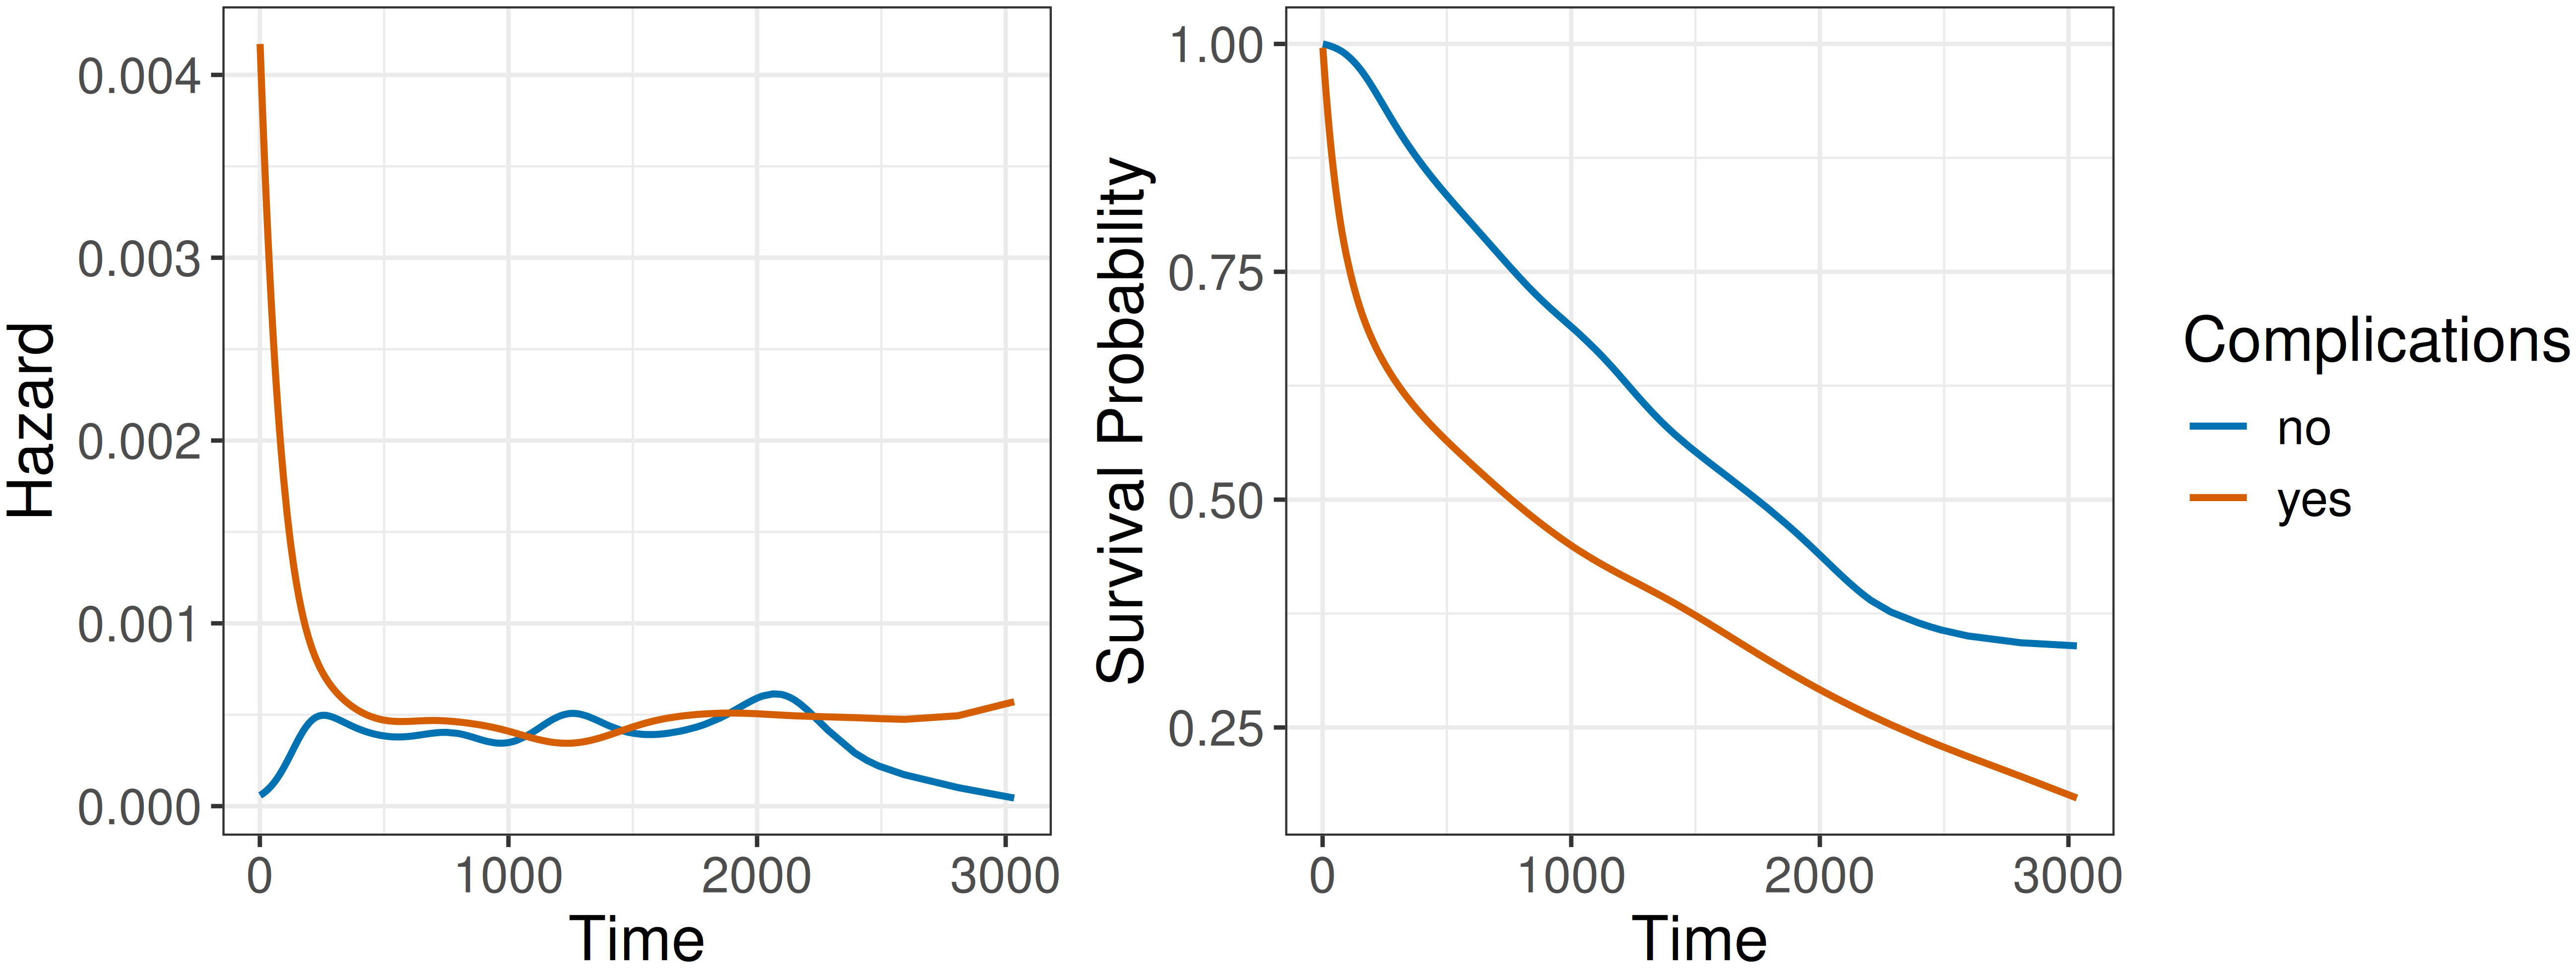
\includegraphics[width=1\linewidth,height=\textheight,keepaspectratio]{Figures/evaluation/fig-p2c8-hazard-surv-complications.png}

}

\caption{\label{fig-p2c8-hazard-surv-complications}Estimated hazard
(left) and survival probability (right) for the \texttt{tumor} dataset,
stratified by the presence or absence of surgical complications. The
hazard curves cross at multiple points, while the survival probability
curves remain consistently separated.}

\end{figure}%

\subsection{Competing risks}\label{competing-risks}

Discrimination measures in competing risks settings are typically
defined at the cause-specific level, with overall measures being
obtained by aggregating across event types if required (Alberge et al.
2025; Bender et al. 2021; C. Lee et al. 2018).\index{competing risks}

A simplistic extension of concordance is based on defining a pair
\((i,j)\) as comparable for event \(\tilde{q}\) if

\[
t_i < t_j \wedge q_i = \tilde{q},
\]

where \(q_i \in \{0,\ldots,Q\}\) is the event experienced by observation
\(i\) and \(q_i = 0\) indicates censoring. In words, observations \(i\)
and \(j\) are comparable if \(i\) experienced the event of interest
before \(j\) experienced any event or was censored. If
\(q_i \ne \tilde{q}\), then observation \(i\) either experienced a
competing event or was censored; neither scenario provides useful
information about discrimination for event \(\tilde{q}\), so such pairs
are excluded from being comparable.

A cause-specific concordance
measure\index{concordance index!cause-specific} for cause
\(\tilde{q} \in \{1,\ldots,Q\}\) can be written as,

\[
C_{\tilde{q}}(\mathbf{\hat{h}}_{\tilde{q}}, \mathbf{q}, \mathbf{t}\mid \tau) = \frac{\sum_{i\neq j} w_{\tilde{q}}(t_i)\mathbb{I}(t_i < t_j, \hat{h}_{\tilde{q},i}(t_i) > \hat{h}_{\tilde{q},j}(t_i), t_i < \tau, q_i = \tilde{q})}{\sum_{i\neq j}w_{\tilde{q}}(t_i)\mathbb{I}(t_i < t_j, t_i < \tau, q_i = \tilde{q})},
\]

where
\(\mathbf{\hat{h}}_{\tilde{q}} = (\hat{h}_{\tilde{q},1} \ \hat{h}_{\tilde{q},2} \cdots \hat{h}_{\tilde{q},n})^\top\)
are the predicted cause-specific hazard functions
(\ref{eq-cause-specific-hazard}) for event \(\tilde{q}\),
\(\boldsymbol{\mathbf{q}} = ({q}_1 \ {q}_2 \cdots {q}_{n})^\top\) is the
vector of observed causes, and \(w_{\tilde{q}}(t_i)\) are cause-specific
weights.

This measure evaluates if, among individuals still at risk at \(t_i\),
those with higher predicted risk of event \(\tilde{q}\) tend to
experience that event earlier. This approach only applies naturally to
models that provide cause-specific hazard predictions.

An alternative is suggested by Wolbers et al. (2014). For event of
interest \(\tilde{q} \in \{1,\ldots,Q\}\), the concordance probability
of interest is:

\[
\Pr(\hat{r}_{\tilde{q};i} > \hat{r}_{\tilde{q};j} \mid q_i = \tilde{q} \wedge (t_i < t_j \vee q_j \in \{1,\ldots,Q\} \setminus \{\tilde{q}\}))
\]

for cause-specific risk predictions
\(\hat{r}_{\tilde{q};i}, \hat{r}_{\tilde{q};j}\). That is, a prediction
is concordant if the observation experiencing event \(\tilde{q}\)
receives a larger predicted risk than an observation that either
experiences the event later or experiences a competing event. Wolbers et
al. (2014) relates this to the standard concordance definition by
defining:

\[
t_{\tilde{q};i} :=
\begin{cases}
t_i, & \text{ if } q_i \in \{0, \tilde{q}\},\\
\infty, & \text{ if } q_i \in \{1, \ldots,Q\} \setminus \{\tilde{q}\},
\end{cases}
\]

for event \(\tilde{q}\) and some observation \(i\) with observed outcome
time \(t_i\). That is, observations experiencing competing events are
treated as if the event of interest could never subsequently occur.
Under this definition, the probability to estimate is the familiar
(\ref{eq-cindex-prob}),

\[
\Pr(\hat{r}_{\tilde{q};i} > \hat{r}_{\tilde{q};j} \mid t_{\tilde{q};i} < t_{\tilde{q};j}).
\]

Estimating this quantity relies on the cumulative incidence
function\index{cumulative incidence function} (\ref{eq-cif}) for the
event of interest, together with inverse probability of censoring
weighting (Section~\ref{sec-surv-ipcw}) to account for censored
observations (Wolbers et al. 2014). Implementations are readily
available in open-source software (such as Ulla B. Mogensen, Ishwaran,
and Gerds 2012).

\subsection{Handling truncation}\label{handling-truncation}

If one were to ignore left-truncation \index{truncation!left} and apply
(\ref{eq-cindex}) directly, the result is an estimator that converges in
probability to,

\begin{equation}\phantomsection\label{eq-cindex-lt-naive}{
\Pr(\hat{r}_i > \hat{r}_j  \mid  t_i < t_j, t_i \geq t^\ell_i, t_j \geq t^\ell_j),
}\end{equation}

where \(t^\ell_i\) and \(t^\ell_j\) denote the left-truncation times for
observations \(i\) and \(j\) respectively (equal to \(0\) if the
observation is not left-truncated) (Hartman et al. 2022). The limiting
quantity (\ref{eq-cindex-lt-naive}) depends on the truncation
distribution and may therefore introduce bias. The conditioning event on
the right-hand side of (\ref{eq-cindex-lt-naive}),

\[
t_i < t_j \wedge t_i \geq t^\ell_i \wedge t_j \geq t^\ell_j,
\]

holds true even when observation \(i\) experiences the event before
observation \(j\) becomes observable,

\[
t_i < t_j^\ell < t_j.
\]

In this situation, the comparison is not meaningful as observation \(j\)
could never have experienced the event before observation \(i\) due to
delayed entry\index{delayed entry}. To avoid non-overlapping
comparisons, one can instead condition on the left-truncation time of
the comparison observation (Hartman et al. 2022):

\begin{equation}\phantomsection\label{eq-cindex-lt-adjusted}{
\Pr(\hat{r}_i > \hat{r}_j  \mid  t_i < t_j, t_i \geq t^\ell_i, t_i \geq t^\ell_j).
}\end{equation}

Observe that \(t_j \ge t_j^\ell\) in (\ref{eq-cindex-lt-naive}) is
replaced by \(t_i \ge t_j^\ell\) in (\ref{eq-cindex-lt-adjusted}),
ensuring that the event time of observation \(i\) occurs after the
left-truncation time of observation \(j\). A pair is therefore
comparable if \(t^\ell_j \le t_i < t_j\). An estimator for this quantity
is\index{concordance index!left-truncation}

\begin{equation}\phantomsection\label{eq-concordance-lt}{
C_{LT}(\hat{\mathbf{r}}, \mathbf{t}, \boldsymbol{\delta}, \mathbf{t}^\ell \mid \tau) = \frac{\sum_{i\neq j} \mathbb{I}(t_i < t_j, t_i \geq t^\ell_j, \hat{r}_i > \hat{r}_j, t_i < \tau)\delta_i}{\sum_{i\neq j}\mathbb{I}(t_i < t_j, t_i \geq t^\ell_j, t_i < \tau)\delta_i}.
}\end{equation}

This estimator can be further extended to incorporate a form of inverse
probability weights using the left-truncation distribution to reduce
dependence on the truncation distribution. Estimating such weights in
the presence of left-truncation is technically involved and in practice
(\ref{eq-concordance-lt}) can be found in implementations (Therneau and
Atkinson 2024). However, (\ref{eq-concordance-lt}) should be used with
care, as Hartman et al. (2022) demonstrates that it may actually perform
worse than the naive estimator under certain truncation distributions.
As with all discrimination measures, it is advisable to assess
performance alongside calibration measures (McGough et al. 2021).

\subsection{Interval censoring}\label{interval-censoring-1}

Concordance indices are designed to evaluate how well a model
discriminates between two risk groups. This is a substantial challenge
when there is interval censoring\index{censoring!interval} as the `true'
ranks of observations are unknown. To see this, let \((i,j)\) be two
observations with interval censoring times \((l_i, r_i]\) and
\((l_j, r_j]\) respectively. Pairing these observations can yield one of
six combinations as visualized in Figure~\ref{fig-p2c8-intervals}. Only
the first two combinations result in non-overlapping intervals where it
is clear when observation \(i\) or \(j\) experiences the event first.
For all other cases, a ranking can only be determined either through
conditional probabilities or imputation (Tsouprou 2015; Ying Wu and Cook
2020). After such estimation, interpretation of any metric is difficult,
as it is unclear if the original prediction is being evaluated or the
estimation that went into the evaluation measure.

\begin{figure}

\centering{

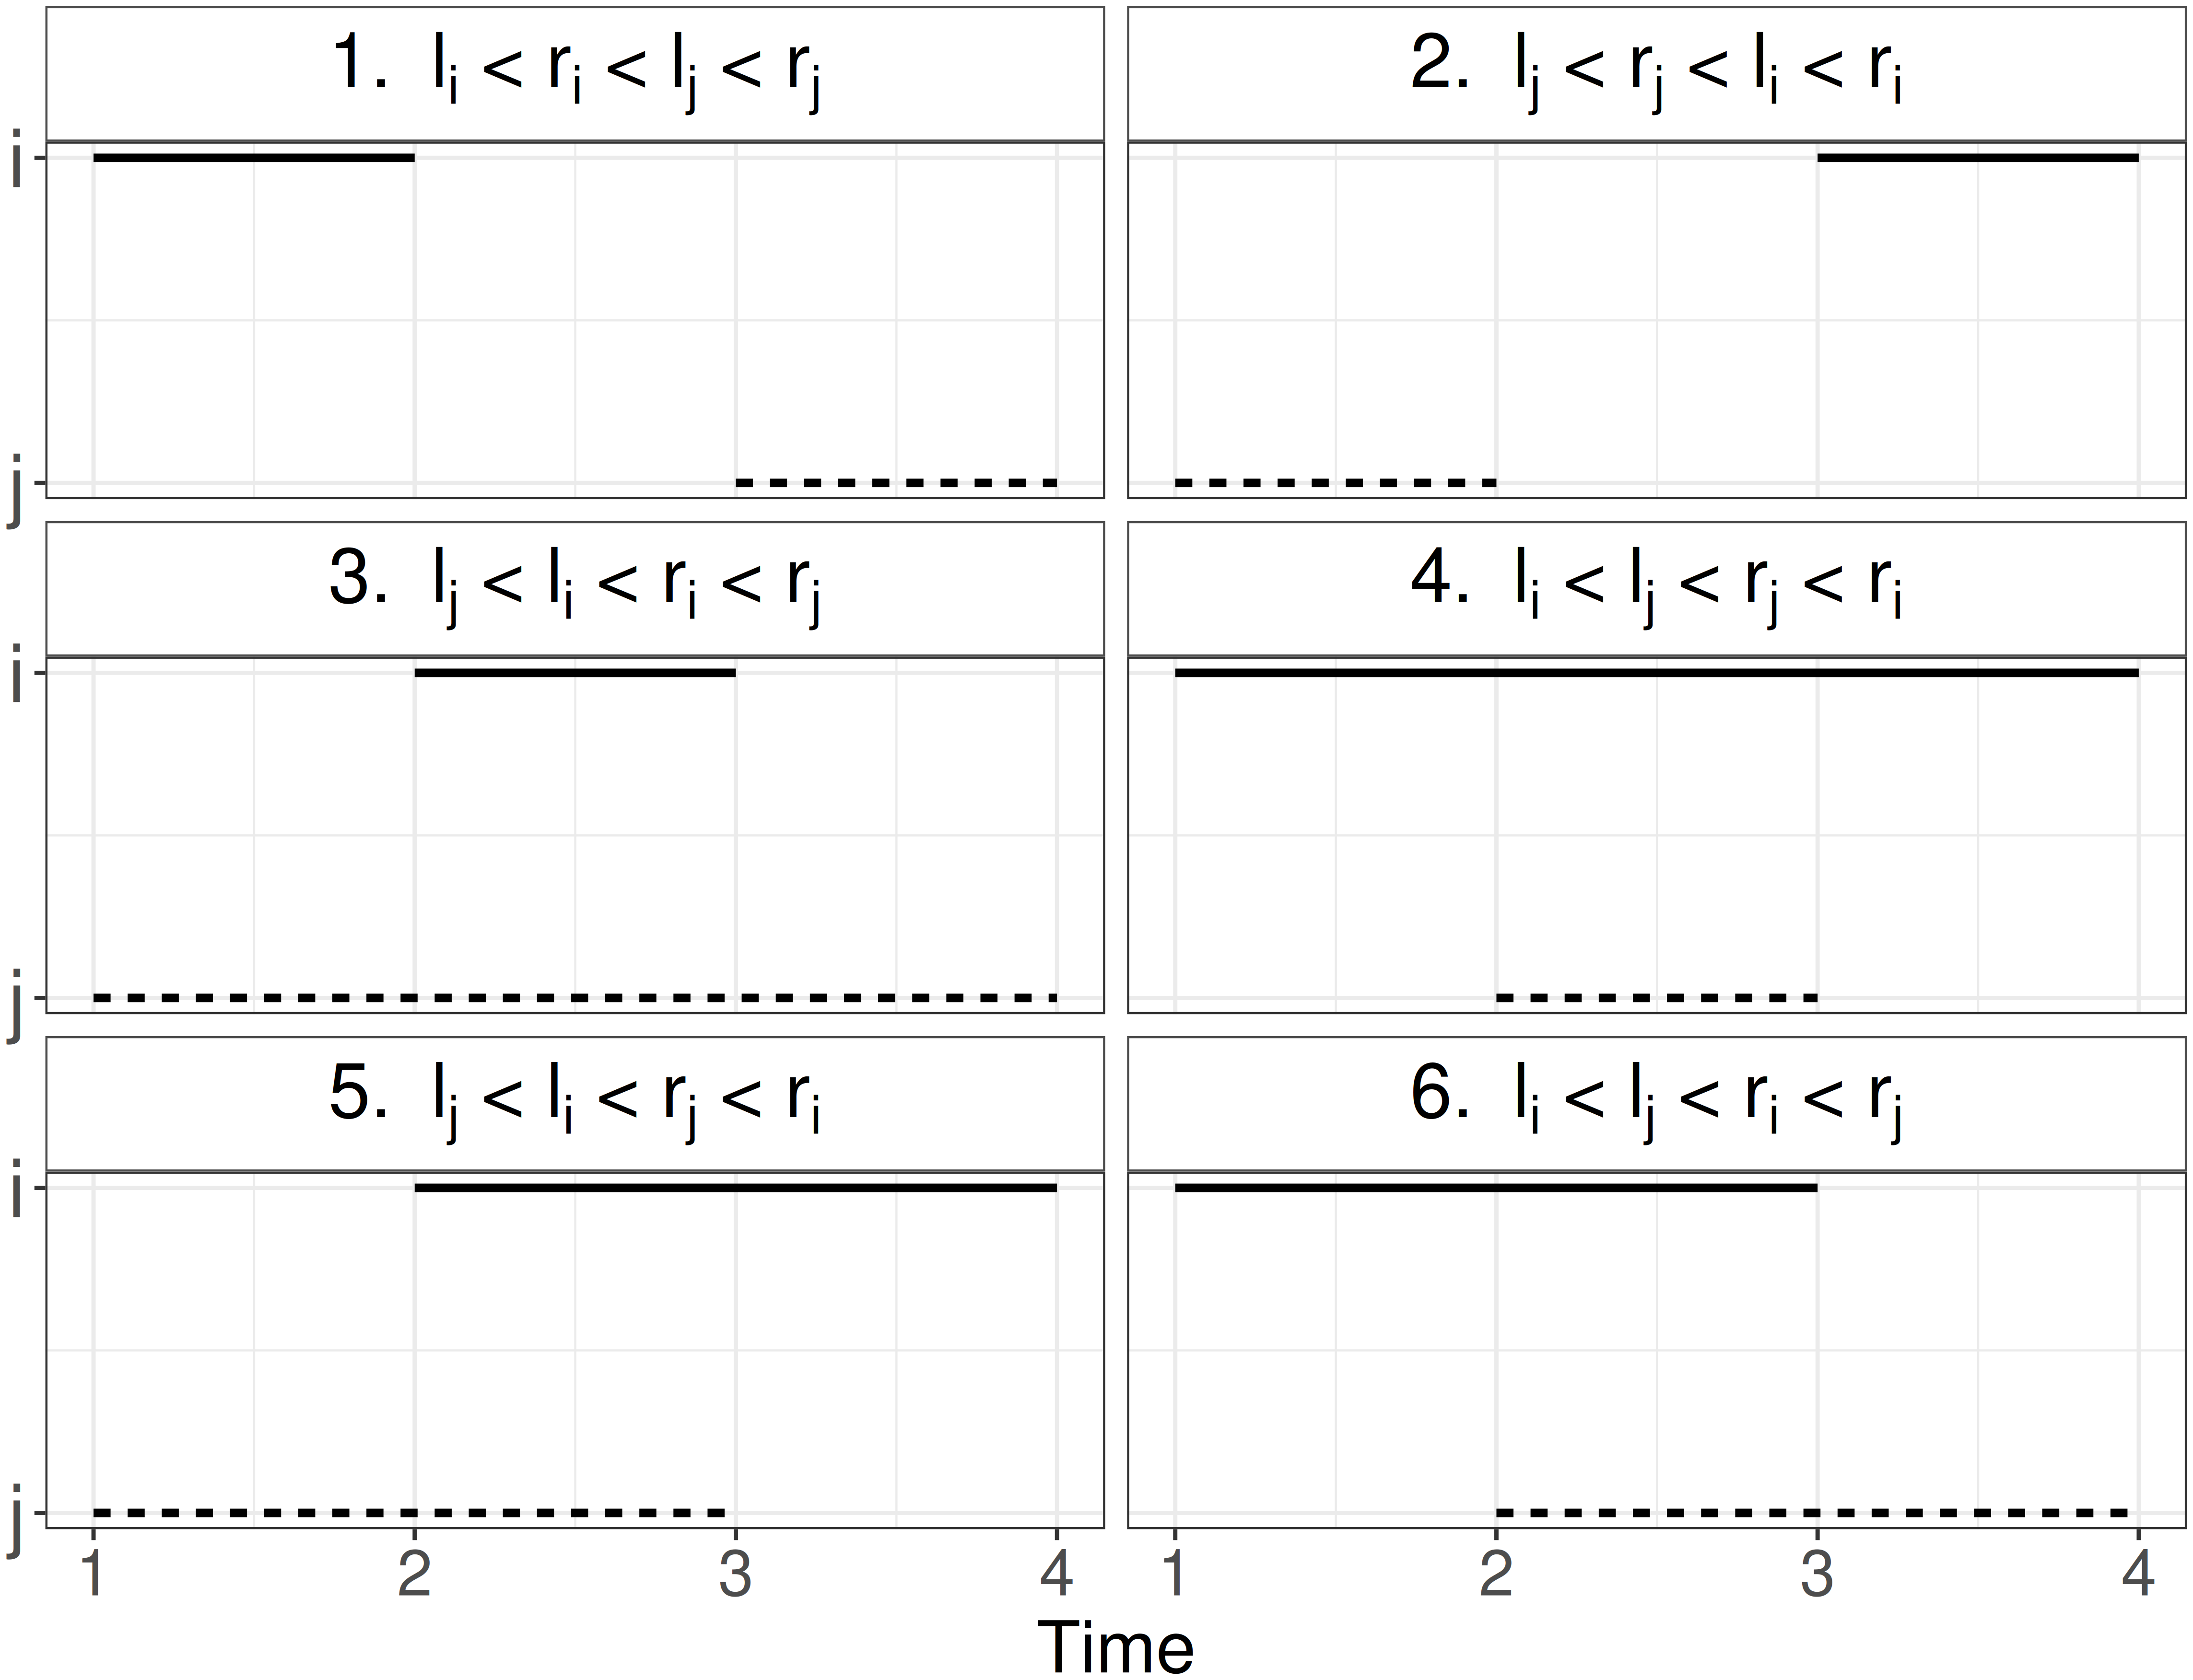
\includegraphics[width=0.9\linewidth,height=\textheight,keepaspectratio]{Figures/evaluation/fig-p2c8-intervals.png}

}

\caption{\label{fig-p2c8-intervals}Combinations of overlapping intervals
for observations \((i,j)\) with interval censoring times
\((l_i, r_i], (l_j, r_j]\) respectively. The first two combinations
result in non-overlapping intervals as \(r_i < l_j\) in the first case
and \(r_j < l_i\) in the second case. For all other combinations, the
intervals are overlapping and it cannot be determined which observation
actually experienced the event first.}

\end{figure}%

\subsection{Choosing a C-index}\label{sec-eval-crank-choose}

With multiple choices of weighting available, choosing a specific
measure might seem daunting. This is complicated by debate in the
literature, reflecting uncertainty in measure choice and interpretation.

When the cutoff \(\tau\) is too small, the chosen measure is only
calculated on early events and as such only provides an estimate that
reflects short-term discrimination rather than overall model
performance. In contrast, when \(\tau\) is too large, then
IPCW\index{inverse probability of censoring weights} measures can be
highly unstable (M. S. Rahman et al. 2017; Uno et al. 2011), for example
the variance of Uno's C\index{concordance index!Uno's C} increases with
increased censoring (Schmid and Potapov 2012). For non-IPCW measures
(such as Harrell's C)\index{concordance index!Harrell's C}, when
\(\tau\) is too large the central estimate provided by the measure is
heavily affected by the proportion of censoring, though the variance may
be more stable (M. S. Rahman et al. 2017).

When there is no clear a priori choice of \(\tau\), a common rule of
thumb is to set \(\tau\) to be the time point at which 80\% of the
observations have experienced the event or censoring, which is the 80th
order statistic from ordered outcome (event or censoring) times:

\[
t_{(1)} \leq t_{(2)} \leq \ldots \leq t_{(n)}; \quad \tau = t_{(\lceil 0.8n \rceil)}.
\]

Even with a suitable choice of \(\tau\), the C-index will always be
highly dependent on censoring within a dataset. Therefore, C-index
values between experiments are not directly comparable; instead,
comparisons are limited to comparing model rankings, for example
conclusions such as ``model A outperformed model B with respect to
Harrell's C in this experiment''.

When a suitable cutoff, \(\tau\), is chosen, all these weightings
perform similarly in many practical settings (M. S. Rahman et al. 2017;
Schmid and Potapov 2012). To illustrate this,
Figure~\ref{fig-p2c8-cindex} uses the \texttt{lung} dataset (Loprinzi et
al. 1994) to compare three weighting schemes across a range of cutoffs.
The vertical lines indicate the times at which 60\%, 70\%, 80\% and 90\%
of observations respectively have experienced the event or been
censored. The measures are almost identical and at their peak difference
only differ by 0.02.

\begin{figure}

\centering{

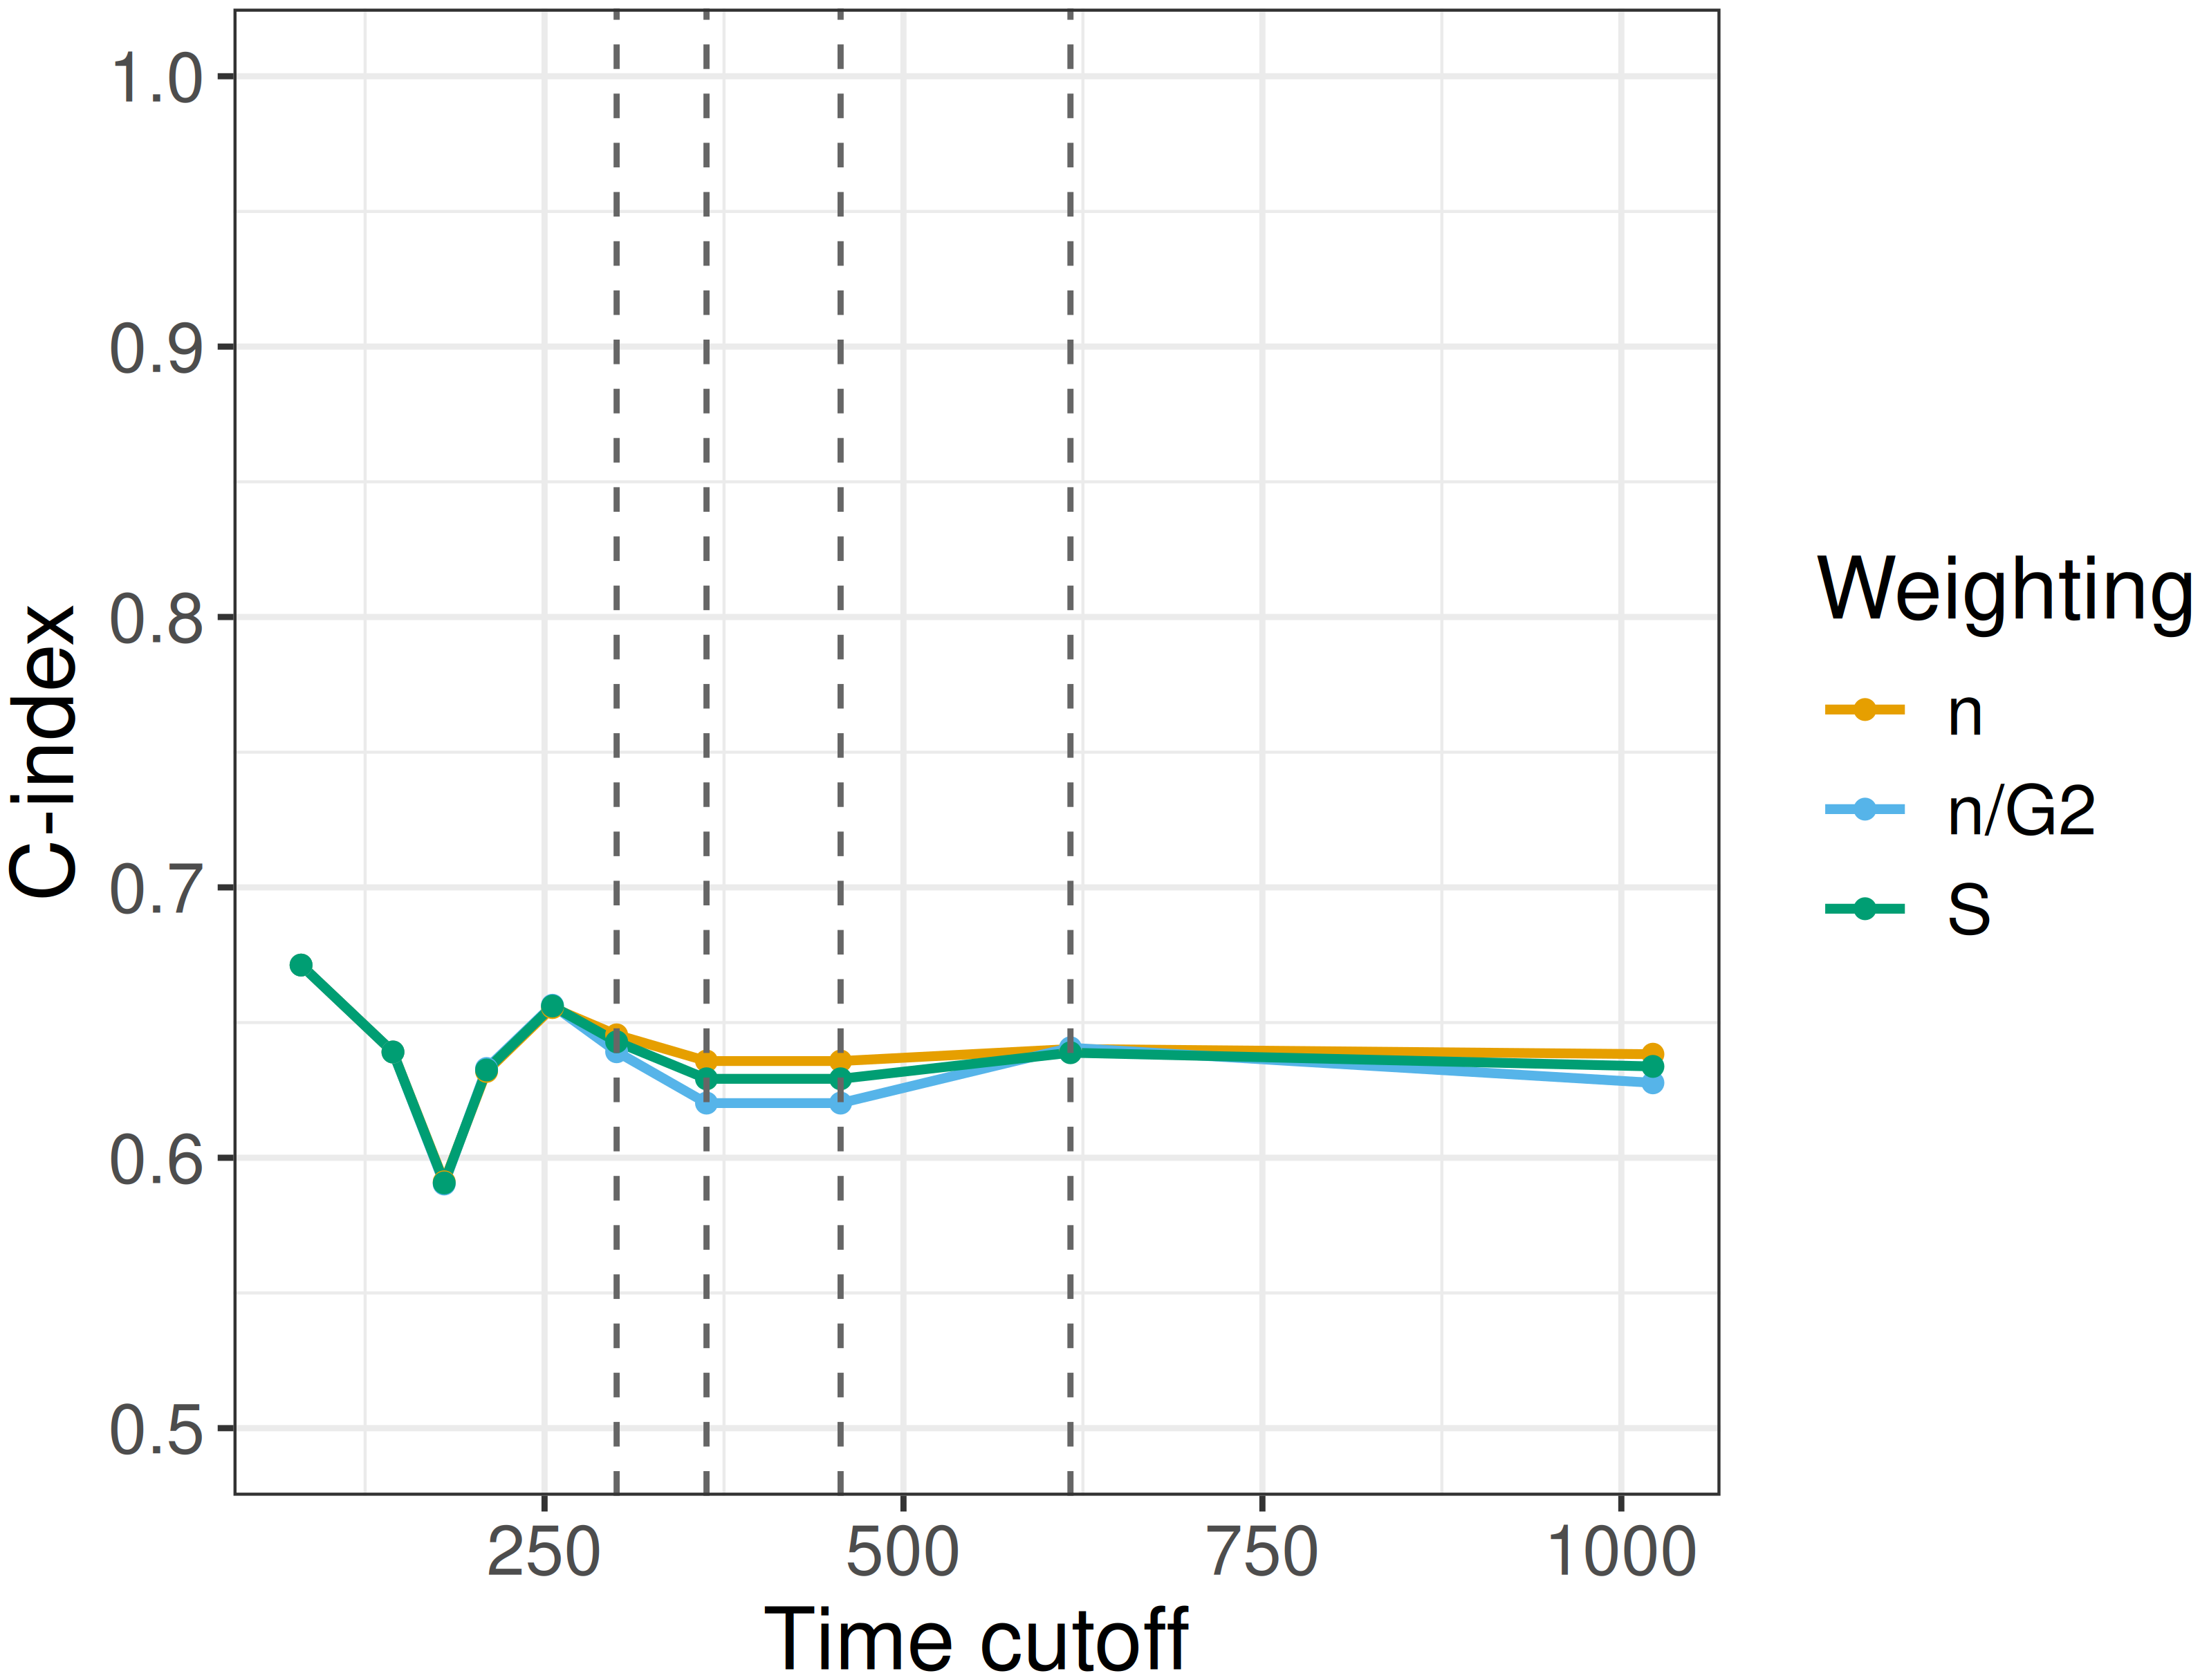
\includegraphics[width=0.7\linewidth,height=\textheight,keepaspectratio]{Figures/evaluation/fig-p2c8-cindex.png}

}

\caption{\label{fig-p2c8-cindex}Three choices of weighting schemes for
the C-index. The orange line is Harrell's C, blue line is Uno's C, and
the green line is the Peto-Wilcoxon weighted C-index. The vertical lines
indicate the times at which 60\%, 70\%, 80\% and 90\% of observations
respectively have experienced the event or been censored.}

\end{figure}%

In practice, given a suitable \(\tau\), all C-index metrics provide an
intuitive measure of discrimination and as such the choice of C-index is
less important than the transparency in reporting. Uno's C and Harrell's
C are both common in the literature; see
Chapter~\ref{sec-choosing-measures} for further discussion.

The number of concordance indices, and the complexity surrounding them,
means that it is not uncommon to see `C-hacking' in the literature
(Sonabend, Bender, and Vollmer 2022)\index{C-hacking}. C-hacking is the
deliberate, unethical procedure of calculating multiple C-indices and
selectively reporting one or more results to promote a particular model,
while ignoring any negative findings. For example, calculating Harrell's
C and Uno's C but only reporting the measure showing that a particular
model performs better than another (even if the other metric shows the
reverse effect). To avoid `C-hacking':

\begin{enumerate}
\def\labelenumi{\arabic{enumi}.}
\tightlist
\item
  the exact choice of C-index should be made before experiments and
  clearly reported including any weights, handling of ties, and cutoffs;
  and
\item
  any transformations from distribution to ranking predictions
  (Chapter~\ref{sec-survtsk}) should be chosen and clearly described
  before starting experiments.
\end{enumerate}

\section{Area under the curve}\label{sec-auc}

The area under the curve (AUC)\index{area under the curve} measure
specifically refers to the area under the curve obtained by plotting the
true positive rate (TPR)\index{true positive rate} against the false
positive rate (FPR)\index{false positive rate} (one minus true negative
rate\index{true negative rate}) across different decision thresholds.
This measure is sometimes referred to as the AUROC as the plot of true
positive rate against false positive rate is known as the receiver
operating characteristic (ROC) curve, hence area under the ROC. In
binary classification\index{classification!binary}, the area under the
curve can be interpreted as the probability that a randomly selected
positive observation receives a higher predicted probability than a
randomly selected negative
observation\index{positive class}\index{negative class}; this is the
same interpretation as the concordance index\index{concordance index} in
the binary classification setting (up to handling of ties) (Uno et al.
2011).

To elucidate the AUC, consider the binary classification problem of
predicting whether it will rain tomorrow. This leads to four possible
deterministic outcomes which can be visualized in a confusion
matrix\index{confusion matrix} (Table~\ref{tbl-confusion-classif}).

\begin{longtable}[]{@{}lll@{}}
\caption{Binary classification confusion matrix for the deterministic
task: will it rain
tomorrow?}\label{tbl-confusion-classif}\tabularnewline
\toprule\noalign{}
\endfirsthead
\endhead
\bottomrule\noalign{}
\endlastfoot
& Observed rain & Observed no rain \\
Predicted rain & True positive (TP) & False positive (FP) \\
Predicted no rain & False negative (FN) & True negative (TN) \\
\end{longtable}

Across an entire dataset, one can count the total number of true
positives (TPs)\index{true positive} and so on and then define the true
positive rate and true negative rate (TNR)\index{true negative rate} as:

\[
\mathrm{TPR} = \frac{\mathrm{TPs}}{\mathrm{TPs} + \mathrm{FNs}}, \quad \mathrm{TNR} = \frac{\mathrm{TNs}}{\mathrm{TNs} + \mathrm{FPs}}, \quad \mathrm{FPR} = 1 - \mathrm{TNR}.
\]

Now consider probabilistic classification where a model predicts
\(\Pr(\mathrm{rain}) = \hat{p}\) for some \(\hat{p} \in [0,1]\). To
convert probabilistic predictions\index{classification!probabilistic}
into deterministic labels, a decision threshold \(\alpha\) must be
chosen such that

\[
\hat{y} =
\begin{cases}
\text{Rain}, & \text{ if } \hat{p} \ge \alpha, \\
\text{No rain}, & \text{ if } \hat{p} < \alpha.
\end{cases}
\]

The receiver operating characteristic curve plots the true positive rate
against the false positive rate for all possible threshold values. The
AUC is the area under this curve\index{area under the curve} and is in
the range \([0,1]\) with larger values preferred. In
Figure~\ref{fig-p2c8-rocs}, a perfect classifier is shown by the yellow
line, which goes through the top-left corner of the graph. This optimal
curve corresponds to a model for which there exists a threshold at which
all positive labels are correctly identified (TPR = 1) and no negative
labels are incorrectly classified (FPR = 0). In practice, achieving
perfect separation is rare, and different thresholds produce different
trade-offs between true positive and false positive rates. Hence
performance is considered across multiple thresholds. The orange curve
running along \(y=x\) represents a random guess classifier (`a coin
toss') where at every threshold there is an equal rate of true positives
and false positives. The other two curves represent models that are
better than a random guess but do not reach the performance of the
optimal classifier.

\begin{figure}

\centering{

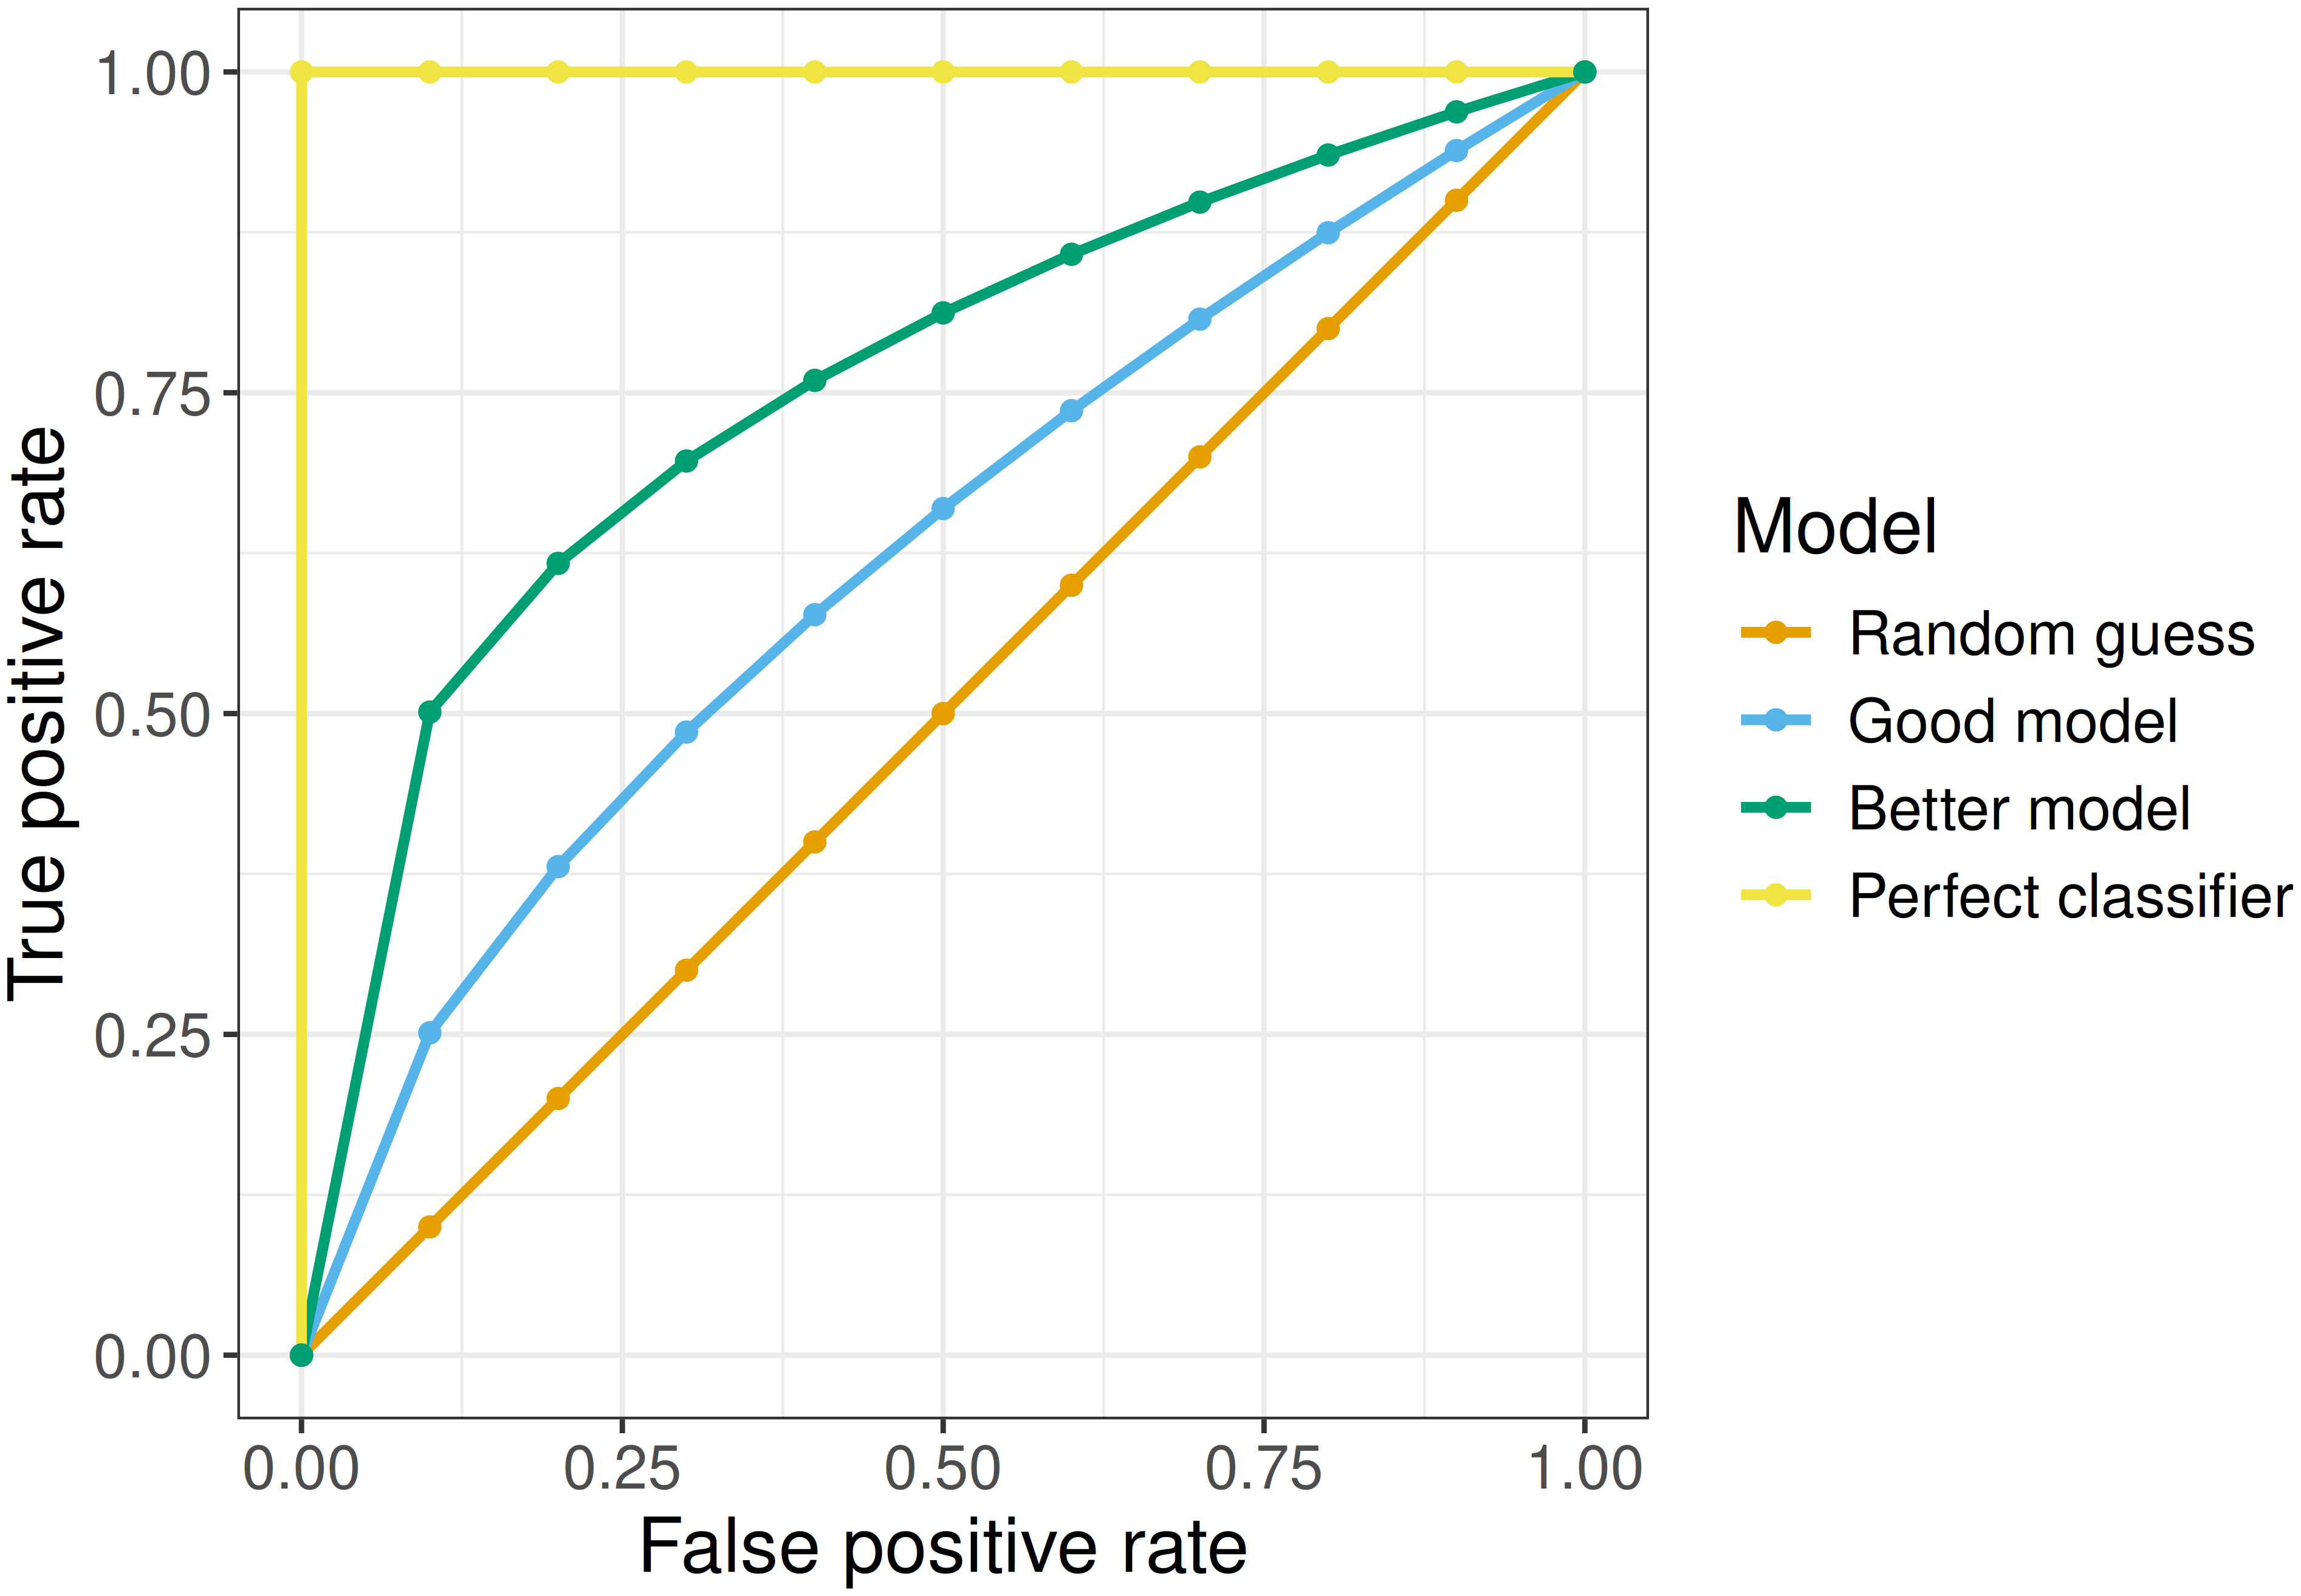
\includegraphics[width=0.7\linewidth,height=\textheight,keepaspectratio]{Figures/evaluation/fig-p2c8-rocs.png}

}

\caption{\label{fig-p2c8-rocs}ROC Curves for a binary classification
example. The yellow curve is a perfect classifier that goes through the
top-left corner, the orange line on y=x is equivalent to a random guess,
the blue and green curves represent two models, with the green one
performing slightly better.}

\end{figure}%

\subsection{True positives and negatives in survival
analysis}\label{true-positives-and-negatives-in-survival-analysis}

To apply the AUC in a survival analysis setting, one must define a true
positive and true negative. This presents two challenges: first,
determining \emph{if} an observation outcome is considered `positive' or
`negative'; and second, determining \emph{when} an outcome is positive
or negative. Following terminology from medical statistics, it is common
to term an observation a `case'\index{area under the curve!case/control}
if they experienced the event of interest or a `control' otherwise. Let
\(\tau\) be a time point of interest and let \(i\) be an observation
with outcome \((t_i, \delta_i)\), then there are three possible
scenarios:

\begin{enumerate}
\def\labelenumi{\arabic{enumi}.}
\tightlist
\item
  The observation has experienced the event by \(\tau\), in which case
  they are a `case': \(t_i \le \tau \wedge \delta_i = 1\);
\item
  The observation has not experienced any outcome by \(\tau\) and is
  considered a `control': \(t_i > \tau\);
\item
  The observation has been censored by \(\tau\) and is neither a `case'
  nor `control' (accounted for below with IPCW):
  \(t_i \le \tau \wedge \delta_i = 0\).
\end{enumerate}

Similarly to the probabilistic classification case, in a survival
analysis setting one must assign a relative risk\index{relative risk}
prediction to a label (case or control). Let \(\hat{r}_i\) be a risk
prediction for observation \(i\) with the usual interpretation that
higher values yield higher risk, and let \(\alpha\) be a cutoff to
threshold the prediction, such that \(\hat{r}_i \ge \alpha\) assigns the
`case' label, otherwise `control'. The confusion
matrix\index{confusion matrix} for relative risk predictions is
presented in Table~\ref{tbl-confusion-survival}.

\begin{longtable}[]{@{}lll@{}}
\caption{Confusion matrix at time \(\tau\) for risk threshold \(\alpha\)
for an observation \(i\) with relative risk prediction
\(\hat{r}_i\).}\label{tbl-confusion-survival}\tabularnewline
\toprule\noalign{}
\endfirsthead
\endhead
\bottomrule\noalign{}
\endlastfoot
& \(t_i \le \tau \wedge \delta_i = 1\) & \(t_i > \tau\) \\
\(\hat{r}_i \ge \alpha\) & True positive (TP) & False positive (FP) \\
\(\hat{r}_i < \alpha\) & False negative (FN) & True negative (TN) \\
\end{longtable}

With these definitions, one can define the time-dependent TPR and TNR
for survival analysis
as\index{true positive rate!time-dependent}\index{true negative rate!time-dependent},

\begin{equation}\phantomsection\label{eq-tpr}{
\mathrm{TPR}_S(\hat{\mathbf{r}}, \mathbf{t}, \boldsymbol{\delta}\mid  \tau, \alpha) = \frac{\sum_i \mathbb{I}(\hat{r}_i \ge \alpha, t_i \le \tau, \delta_i = 1)}{\sum_i \mathbb{I}(t_i \le \tau, \delta_i = 1)},
}\end{equation}

and

\begin{equation}\phantomsection\label{eq-tnr}{
\mathrm{TNR}_S(\hat{\mathbf{r}}, \mathbf{t}\mid  \tau, \alpha) = \frac{\sum_i \mathbb{I}(\hat{r}_i < \alpha, t_i > \tau)}{\sum_i \mathbb{I}(t_i > \tau)}.
}\end{equation}

These definitions correspond to the `cumulative/dynamic' formulations
(Patrick J. Heagerty, Lumley, and Pepe 2000; Patrick J. Heagerty and
Zheng 2005)\index{area under the curve!cumulative/dynamic}. In this
formulation, an observation is considered a case if the event has
occurred at any time up to and including \(\tau\). In contrast, the
incident/dynamic\index{area under the curve!incident/dynamic}
formulation defines cases as individuals who experience the event
\emph{at} time \(\tau\) among those still at risk (Patrick J. Heagerty
and Zheng 2005). The cumulative/dynamic formulation is often more
intuitive to interpret in applied settings (Blanche, Dartigues, and
Jacqmin-Gadda 2013). The cumulative definition of a case aligns
naturally with the survival and cumulative incidence functions, which
describe the probability of an event occurring \emph{by} \(\tau\). In
contrast, the incident definition more closely corresponds to the hazard
function, as it considers events occurring \emph{at} \(\tau\) among
those still at risk.

Similarly to the issues faced by Harrell's
C\index{concordance index!Harrell's C}, (\ref{eq-tpr}) discards censored
observations, which could lead to bias in the measure. As with prior
measures, this can be corrected via IPC
weighting\index{inverse probability of censoring weights}\index{area under the curve!Uno's}
(Uno et al. 2007):

\begin{equation}\phantomsection\label{eq-tpr-ipcw}{
\mathrm{TPR}_{S^*}(\hat{\mathbf{r}}, \mathbf{t}, \boldsymbol{\delta}\mid  \tau, \alpha) = \frac{\sum_i \mathbb{I}(\hat{r}_i \ge \alpha, t_i \le \tau, \delta_i = 1)[\hat{G}_{KM}(t_i)]^{-1}}{\sum_i \mathbb{I}(t_i \le \tau, \delta_i = 1)[\hat{G}_{KM}(t_i)]^{-1}}.
}\end{equation}

This weighting is not required in (\ref{eq-tnr}), as the status of
controls at \(\tau\) is fully observed.

In practice, (\ref{eq-tnr}) and (\ref{eq-tpr-ipcw}) are straightforward
to estimate and yield time-dependent
AUC\index{area under the curve!time-dependent} measures that allow model
performance to be evaluated at multiple time points. For a fixed time
point \(\tau\), \(\operatorname{AUC}(\tau)\) can be estimated
numerically using any standard method for computing the area under a
curve, such as the trapezoidal rule applied to the ROC curve. A single
summary measure up to a cutoff \(\tau^*\) can then be obtained via a
weighted integral over time\index{area under the curve!integrated},

\[
\operatorname{iAUC}(\tau^*) = \int^{\tau^*}_0 \operatorname{AUC}(\tau) w(\tau) \ d\tau,
\]

where \(w\) is a non-negative weighting function normalized to integrate
to one. Popular choices of weights include the density of events over
time, a non-parametric estimate of the survival function, or simply
uniform weighting across time.

A number of time-dependent AUC methods have been derived (such as,
Chambless and Diao 2006; Hung and Chiang 2010; Song and Zhou
2008)\index{area under the curve!Chambless and Diao's}\index{area under the curve!Song and Zhou's}\index{area under the curve!Hung and Chiang's}.
Various surveys on these measures have produced different results
(Blanche, Latouche, and Viallon 2012; Kamarudin, Cox, and
Kolamunnage-Dona 2017; L. Li, Greene, and Hu 2018) with no clear
consensus on how and when these measures should be used. Plotted as a
curve over time, \(\operatorname{AUC}(\tau)\) can reveal where in the
follow-up period a model discriminates well or poorly. However,
reporting these measures quantitatively can present some challenges. A
single reported \(\operatorname{AUC}(\tau)\) is sensitive to the choice
of \(\tau\), and the integrated \(\operatorname{iAUC}(\tau^*)\)
introduces additional analyst choices, in particular regarding the
weighting function \(w\).

For a single time-independent summary, the concordance indices discussed
earlier may be preferable. For a single time-dependent summary with a
clear concordance interpretation and no need to fix a reporting time
point, Antolini's C (Section~\ref{sec-cindex-dep}) may be more natural
as evaluation times are data-driven rather than chosen by the analyst.

\subsection{Competing risks}\label{competing-risks-1}

In a competing risks
setting\index{competing risks}\index{area under the curve!competing risks},
the definitions of true positive rate and true negative rate must be
adapted to handle multiple event types.

For event \(\tilde{q} \in \{1,\ldots,Q\}\), it is natural to define an
observation \(i\) as a case if they experienced the event of interest by
time \(\tau\):

\[
\operatorname{case}_{\tilde{q};i}(t_i, q_i  \mid  \tau) := t_i \le \tau \wedge q_i = \tilde{q}.
\]

Two separate definitions have been proposed for controls (Geloven et al.
2022). The first defines a control as an observation that has not
experienced \emph{any} event at \(\tau\) (Saha and Heagerty 2010):

\[
\operatorname{control}_{\tilde{q};i}^{1}(t_i  \mid  \tau) := t_i > \tau.
\]

The second defines a control as an observation that has not experienced
the \emph{event of interest} by time \(\tau\) but may have experienced a
competing event (Zheng et al. 2012):

\[
\operatorname{control}^2_{\tilde{q};i}(t_i, q_i, \tau) := t_i > \tau \vee (t_i \le \tau \wedge q_i \in \{1,\ldots,Q\} \setminus \{\tilde{q}\}).
\]

Estimation is more complex in this setting and several approaches have
been proposed. For example, Zheng et al. (2012) estimate these
quantities using smoothed estimates of the conditional cumulative
incidence function.

\subsection{Interval censoring}\label{interval-censoring-2}

For interval censoring, there is an intuitive approach to defining the
TPR and TNR
equations\index{censoring!interval}\index{area under the curve!interval-censoring}
although estimating these quantities is quite complex. Let \(i\) be an
observation with interval censoring times \((l_i, r_i]\). One can then
condition (\ref{eq-tpr}) and (\ref{eq-tnr}) to only include a
contribution from observation \(i\) when it is guaranteed the event must
or must not have occurred (J. Li and Ma 2011).

At \(\tau \le l_i\), the event has definitely not occurred, so an
observation is clearly a control:

\[
\operatorname{control}^{IC}_i(\tau) := \tau \le l_i.
\]

When only left-censoring is present in the data, then \(l_i = 0\) and as
such there is no coherent definition of a control for left-censored
observations (similarly to there being no definition of a case for
right-censored observations).

On the other hand, if \(\tau \ge r_i\) then the event has definitely
occurred, and so an observation must be a case:

\[
\operatorname{case}^{IC}_i(\tau) := \tau \ge r_i.
\]

For time points within the censoring interval, \(l_i < \tau \le r_i\),
it is unknown whether an observation is a case or control. Estimating
TPR and TNR under interval censoring therefore requires estimation of
the underlying event-time distribution. Approaches such as the
non-parametric maximum likelihood
estimator\index{non-parametric maximum likelihood estimator} have been
proposed, although these can be computationally challenging to fit and
spline-based methods have also been suggested (Yuan Wu et al. 2020).
Such approaches also require explicit modeling assumptions about the
event-time distribution, which can complicate interpretation of the
resulting performance estimates and make it difficult to use these
methods in practice.

\section{Conclusion}\label{conclusion-4}

\begin{tcolorbox}[enhanced jigsaw, toprule=.15mm, bottomtitle=1mm, opacityback=0, breakable, leftrule=.75mm, title={Key takeaways}, toptitle=1mm, bottomrule=.15mm, colback=white, colframe=quarto-callout-warning-color-frame, titlerule=0mm, opacitybacktitle=0.6, coltitle=black, rightrule=.15mm, left=2mm, colbacktitle=quarto-callout-warning-color!10!white, arc=.35mm]

\begin{itemize}
\tightlist
\item
  Discrimination measures evaluate relative risk predictions by
  assessing if a model can correctly separate observations who are at
  higher or lower risk of the event.
\item
  Care must be taken when interpreting concordance measures as they can
  change substantially with the censoring mechanism and length of
  follow-up. As a result, absolute values are often not comparable
  across datasets or studies.
\item
  Using a concordance index requires selecting a cutoff value and
  weighting scheme. This allows flexibility but also means choices have
  to be clearly justified by practitioners. Without careful selection,
  results from these measures can vary widely between experiment
  iterations. In practice, Harrell's C is often a sensible first choice,
  provided a sensible cutoff is applied to only evaluate the model up to
  a given time point.
\item
  Concordance measures offer some degree of flexibility over different
  patterns in the underlying dataset. For example, measures can be
  extended to capture changes over time, to handle competing risks, and
  other censoring and truncation types.
\item
  Discrimination measures should rarely be used to evaluate predictions
  on their own as there is often a trade-off between discrimination and
  calibration, which is discussed in the next chapter.
\end{itemize}

\end{tcolorbox}

\begin{tcolorbox}[enhanced jigsaw, toprule=.15mm, bottomtitle=1mm, opacityback=0, breakable, leftrule=.75mm, title={Further reading}, toptitle=1mm, bottomrule=.15mm, colback=white, colframe=quarto-callout-tip-color-frame, titlerule=0mm, opacitybacktitle=0.6, coltitle=black, rightrule=.15mm, left=2mm, colbacktitle=quarto-callout-tip-color!10!white, arc=.35mm]

\begin{itemize}
\tightlist
\item
  The work of Patrick J. Heagerty, Lumley, and Pepe (2000) and Patrick
  J. Heagerty and Zheng (2005) underpinned many later developments in
  time-dependent AUCs. These were touched on briefly in this chapter but
  readers may want to explore these further for more detail and in
  particular to learn about incident/dynamic versus cumulative/dynamic
  AUC definitions.
\item
  Royston and Sauerbrei (2004) present a concordance measure now known
  as Royston's D, which M. S. Rahman et al. (2017) recommend for its
  interpretability. However, this measure does not appear widely used in
  practice and as such was not discussed in this chapter.
\item
  Avati et al. (2020) consider an alternative AUC statistic based on the
  area under the precision-recall curve (AUC-PR). AUC-PR is increasingly
  common in machine learning literature as it may perform better when
  classes are imbalanced.
\end{itemize}

\end{tcolorbox}

\chapter{Calibration}\label{sec-eval-distr-calib}

In the survival analysis context, calibration\index{calibration}
measures evaluate the \emph{average} quality of predicted distributions.
Calibration and discrimination\index{discrimination} emphasize different
aspects of predictive performance. A model with good discrimination may
correctly rank observations while still producing systematically biased
probability estimates. Conversely, a well-calibrated model may produce
accurate population-level predictions but might not separate individual
observations well.

The literature on calibration measures for survival analysis is
comparatively limited (M. S. Rahman et al. 2017), reflecting both
conceptual and methodological challenges (Van Houwelingen 2000). Unlike
metrics that evaluate predictions at the level of individual
observations, calibration assesses the average agreement across the
population. Whereas other measures can accommodate censoring through a
combination of reweighting and dynamic restriction of the risk set,
calibration requires a principled way to incorporate censored
observations when estimating the population-level average. The majority
of research on survival calibration measures has focused on
recalibrating Cox proportional hazards (PH) models (Demler, Paynter, and
Cook 2015; Van Houwelingen 2000). However, these methods are considered
out of scope for this book, which focuses on measures applicable across
all machine learning models.

A useful taxonomy of calibration measures separates them into point
calibration and distributional calibration methods (Andres et al.
2018)\index{calibration!point}\index{calibration!distributional}. Point
calibration evaluates predictions at a single time point. For these
measures to represent a useful quantity, the prediction horizon must be
carefully chosen. Often this is taken to be a practically meaningful
time point, for example the `5-year survival
probability'\index{t-year survival probability@$\tau$-year survival probability}
(Section~\ref{sec-calib-chi}), or the observed event time for each
individual (Section~\ref{sec-alpha}). Point calibration methods are most
useful when there is a clear choice of time point where the prediction
should be optimized and when calibration at other time points may be
poorer or unknown; for example, when using reductions
(Chapter~\ref{sec-ipcw-reduction}). Distributional calibration measures
evaluate the predicted distribution across all time points
(Section~\ref{sec-calib-prob}). These may be preferred when the goal is
to predict and interpret the full survival distribution and calibration
across the entire curve is required.

\section{Point calibration}\label{sec-eval-distr-calib-point}

As above, point calibration measures evaluate distributions at a single
time point, usually a fixed time-horizon or the observed outcome time;
these settings are discussed in turn.

\subsection{Chi-squared methods}\label{sec-calib-chi}

Calibration at a single time point effectively reduces survival
prediction to a binary classification problem, where the outcome is
defined by whether the event has occurred by time \(\tau\). A common
calibration test in the binary classification literature is the
Hosmer-Lemeshow test (Hosmer and Lemeshow 1980)\index{Hosmer-Lemeshow}.
Observations are ordered by predicted event probability and divided into
approximately equal-sized groups (often deciles), such that observations
with similar predicted probabilities are placed in the same bin. The
expected and observed number of events in each group are compared using
the test statistic:

\[
\chi^2_{HL} = \sum^G_{g=1} \frac{(o_g - e_g)^2}{n_g\hat{p}_g(1 - \hat{p}_g)},
\]

where \(G\) is the number of groups, \(o_{g}\) and \(e_{g}\) are the
observed and expected number of events in group \(g\), \(n_g\) is the
number of observations in group \(g\) (usually \(n_g = n/G\)), and
\(\hat{p}_g\) is the average predicted probability of event in each
group. Under the null hypothesis, the test statistic follows a
\(\chi^2_{G-2}\) distribution.\index{chi-squared@chi-squared, $\chi^2$}

The most common adaptation to survival analysis appears to be the
Nam-D'Agostino statistic (D'Agostino and Nam
2003)\index{Hosmer-Lemeshow!Nam-D'Agostino}. Let
\(\bar{\hat{S}}_g(\tau), \bar{\hat{F}}_g(\tau)\) be the average
predicted survival and cumulative distribution functions respectively
evaluated at \(\tau\) for group \(g\), and let \(\hat{F}_{g;KM}\) denote
the cumulative distribution function implied by the Kaplan-Meier
estimator fit within group \(g\), then
\(o_g(\tau) = \hat{F}_{g;KM}(\tau)n_g\) and
\(e_g(\tau) = \bar{\hat{F}}_{g}(\tau)n_g\), giving the test statistic:

\begin{equation}\phantomsection\label{eq-hosmer-nd}{
\chi^2_{ND}(\tau) = \sum^G_{g=1} \frac{(\hat{F}_{g;KM}(\tau)n_g - \bar{\hat{F}}_{g}(\tau)n_g)^2}{n_g\bar{\hat{F}}_{g}(\tau)\bar{\hat{S}}_{g}(\tau)},
}\end{equation}

which follows \(\chi^2_{G-1}\) under the null. This method can evaluate
predictions from any survival model, making it more flexible than other
methods (Demler, Paynter, and Cook 2015). Given the dependence on
non-parametric estimators, analogous constructions may be possible
beyond single-event, right-censored settings by substituting appropriate
estimators; for example, in the competing risks setting by replacing
\(\hat{F}_{g;KM}\) with cause-specific CIFs and using the Aalen-Johansen
estimator\index{Aalen-Johansen estimator} to estimate the observed event
probabilities. However, these extensions appear to be less established
in the literature. Similarly, extension to other censoring and
truncation types may follow using the non-parametric estimator
adaptations discussed in Section~\ref{sec-surv-estimation-non-param}.

Analysis of (\ref{eq-hosmer-nd}) indicates that the proportion of Type I
errors increases with higher proportions of censoring (Demler, Paynter,
and Cook 2015), leading to the
adaptation:\index{Hosmer-Lemeshow!Greenwood-Nam-D'Agostino}

\begin{equation}\phantomsection\label{eq-hosmer-gnd}{
\chi^2_{GND}(\tau) = \sum^G_{g=1} \frac{(\hat{F}_{g;KM}(\tau) - \bar{\hat{F}}_{g}(\tau))^2}{\widehat{\operatorname{Var}}(\hat{F}_{g;KM}(\tau))} \sim \chi^2_{G-1},
}\end{equation}

where
\(\widehat{\operatorname{Var}}(\hat{F}_{g;KM}(\tau)) \equiv \widehat{\operatorname{Var}}(\hat{S}_{g;KM}(\tau))\)
is the Greenwood variance estimator
(\ref{eq-greenwood}).\index{Kaplan-Meier estimator!Greenwood variance}

Theoretically, one could apply (\ref{eq-hosmer-gnd}) across several time
points (accounting for multiple testing) to try to capture calibration
across a range of times; however, this would be inefficient in many
cases. Instead, one might consider D-calibration
(Section~\ref{sec-dcalib}), which generalizes the \(\chi^2\) test idea
to evaluate calibration across the full distribution. Another
possibility for point calibration is to evaluate predicted probabilities
at the observed event time for each observation. While still point-wise,
the evaluation time is observation-specific and therefore spans the
observed event process rather than relying on a single fixed time point.

\subsection{Event frequency calibration}\label{sec-alpha}

Van Houwelingen proposed several measures for calibration, which
evaluate whether ``observed data are consistent with the expected data
from the {[}predicted{]} model'' (Van Houwelingen
2000)\index{calibration!van Houwelingen}. Only one of the proposed
measures generalizes to all survival models that make distribution
predictions, termed here \emph{event frequency
calibration}.\index{calibration!event frequency} Event frequency
calibration defines a model as well-calibrated if, across the entire
test set, the total number of observed events is close to the total
number of events predicted by the model.

Formally, this result can be derived using counting
process\index{counting process} theory (a full derivation is provided in
Appendix 2 of Hosmer Jr, Lemeshow, and May (2011)). The core theoretical
relation underlying event frequency calibration is:

\[
\mathbb{E}[\Delta_i] = \mathbb{E}[H(T_i \mid \mathbf{x}_i)],
\]

that is, for an individual with covariates \(\mathbf{x}_i\) and outcome
time \(T_i\), the expectation of the true cumulative
hazard\index{cumulative hazard function} evaluated at that time equals
the expected number of events for that individual.

Hence, event frequency calibration tests whether the estimated
cumulative hazard satisfies

\[
L_{EF} := \frac{\sum_i \delta_i}{\sum_i \hat{H}(t_i \mid \mathbf{x}_i)} \approx 1,
\]

where \(\hat{H}(t_i \mid \mathbf{x}_i)\) is the cumulative hazard
function from the predicted distribution for observation \(i\) evaluated
at their observed outcome time \(t_i\). The denominator represents the
total number of events expected under the predicted model, which is
compared to the observed total number of events.

To obtain a loss that can be minimized, one may instead consider

\[
L_{EF^1} = \left\lvert 1 - \frac{\sum_i \delta_i}{\sum_i \hat{H}(t_i \mid \mathbf{x}_i)} \right\rvert,
\]

or if a smooth, differentiable function is preferred,

\[
L_{EF^2} = \left(1 - \frac{\sum_i \delta_i}{\sum_i \hat{H}(t_i \mid \mathbf{x}_i)}\right)^2;
\]

both options are minimized at \(0\).

\section{Distributional calibration}\label{sec-calib-prob}

Calibration over a range of time points may be assessed quantitatively
or qualitatively, with graphical methods often favored. Graphical
methods compare the average predicted distribution to the expected
distribution, which can be estimated with a non-parametric estimator,
discussed next.

\subsection{Calibration plots}\label{sec-calib-km}

Calibration plots\index{calibration!plots}, also known as reliability
diagrams, are graphical summaries comparing predicted event
probabilities with the ground truth (Wilks 1990). In binary
classification, the ground truth is represented by observed event
frequencies within each group of interest. In survival analysis,
censoring prevents direct calculation of event frequencies so these must
be estimated. In single-event, right-censored survival analysis, the
natural estimate is the Kaplan-Meier estimator fitted on the evaluation
data, denoted here by
\(\hat{S}^*_{KM}\).\index{calibration!Kaplan-Meier}\index{Kaplan-Meier estimator}

Let \(\hat{S}(\cdot \mid \mathbf{x}_i)\) be the survival function from
the predicted survival distribution for observation \(i\), then the
average predicted survival function at time \(\tau\) is:

\begin{equation}\phantomsection\label{eq-surv-avg}{
\bar{\hat{S}}(\tau) = \frac{1}{n} \sum^{n}_{i = 1} \hat{S}(\tau \mid \mathbf{x}_i).
}\end{equation}

Plotting (\ref{eq-surv-avg}) alongside \(\hat{S}^*_{KM}\) at all
observed time points provides a visual comparison of how closely these
curves align. An example is given in Figure~\ref{fig-p2c9-calibKM}, a
Cox proportional hazards model (CPH), random survival forest (RF), and
relative risk tree (RRT) are all compared to the Kaplan-Meier estimator
(KM). This figure highlights the advantages and disadvantages of this
method. The relative risk tree is clearly poorly calibrated as it
increasingly diverges from the Kaplan-Meier. In contrast, the Cox PH and
random forest are difficult to compare directly, as both models
frequently overlap with each other and the Kaplan-Meier estimator. While
it is possible to say that the Cox PH and random forest are better
calibrated than the risk tree, it is not possible to say which of the
first two is better calibrated and if their observed difference from the
Kaplan-Meier estimate is significant at a given time (when not clearly
overlapping).

\begin{figure}

\centering{

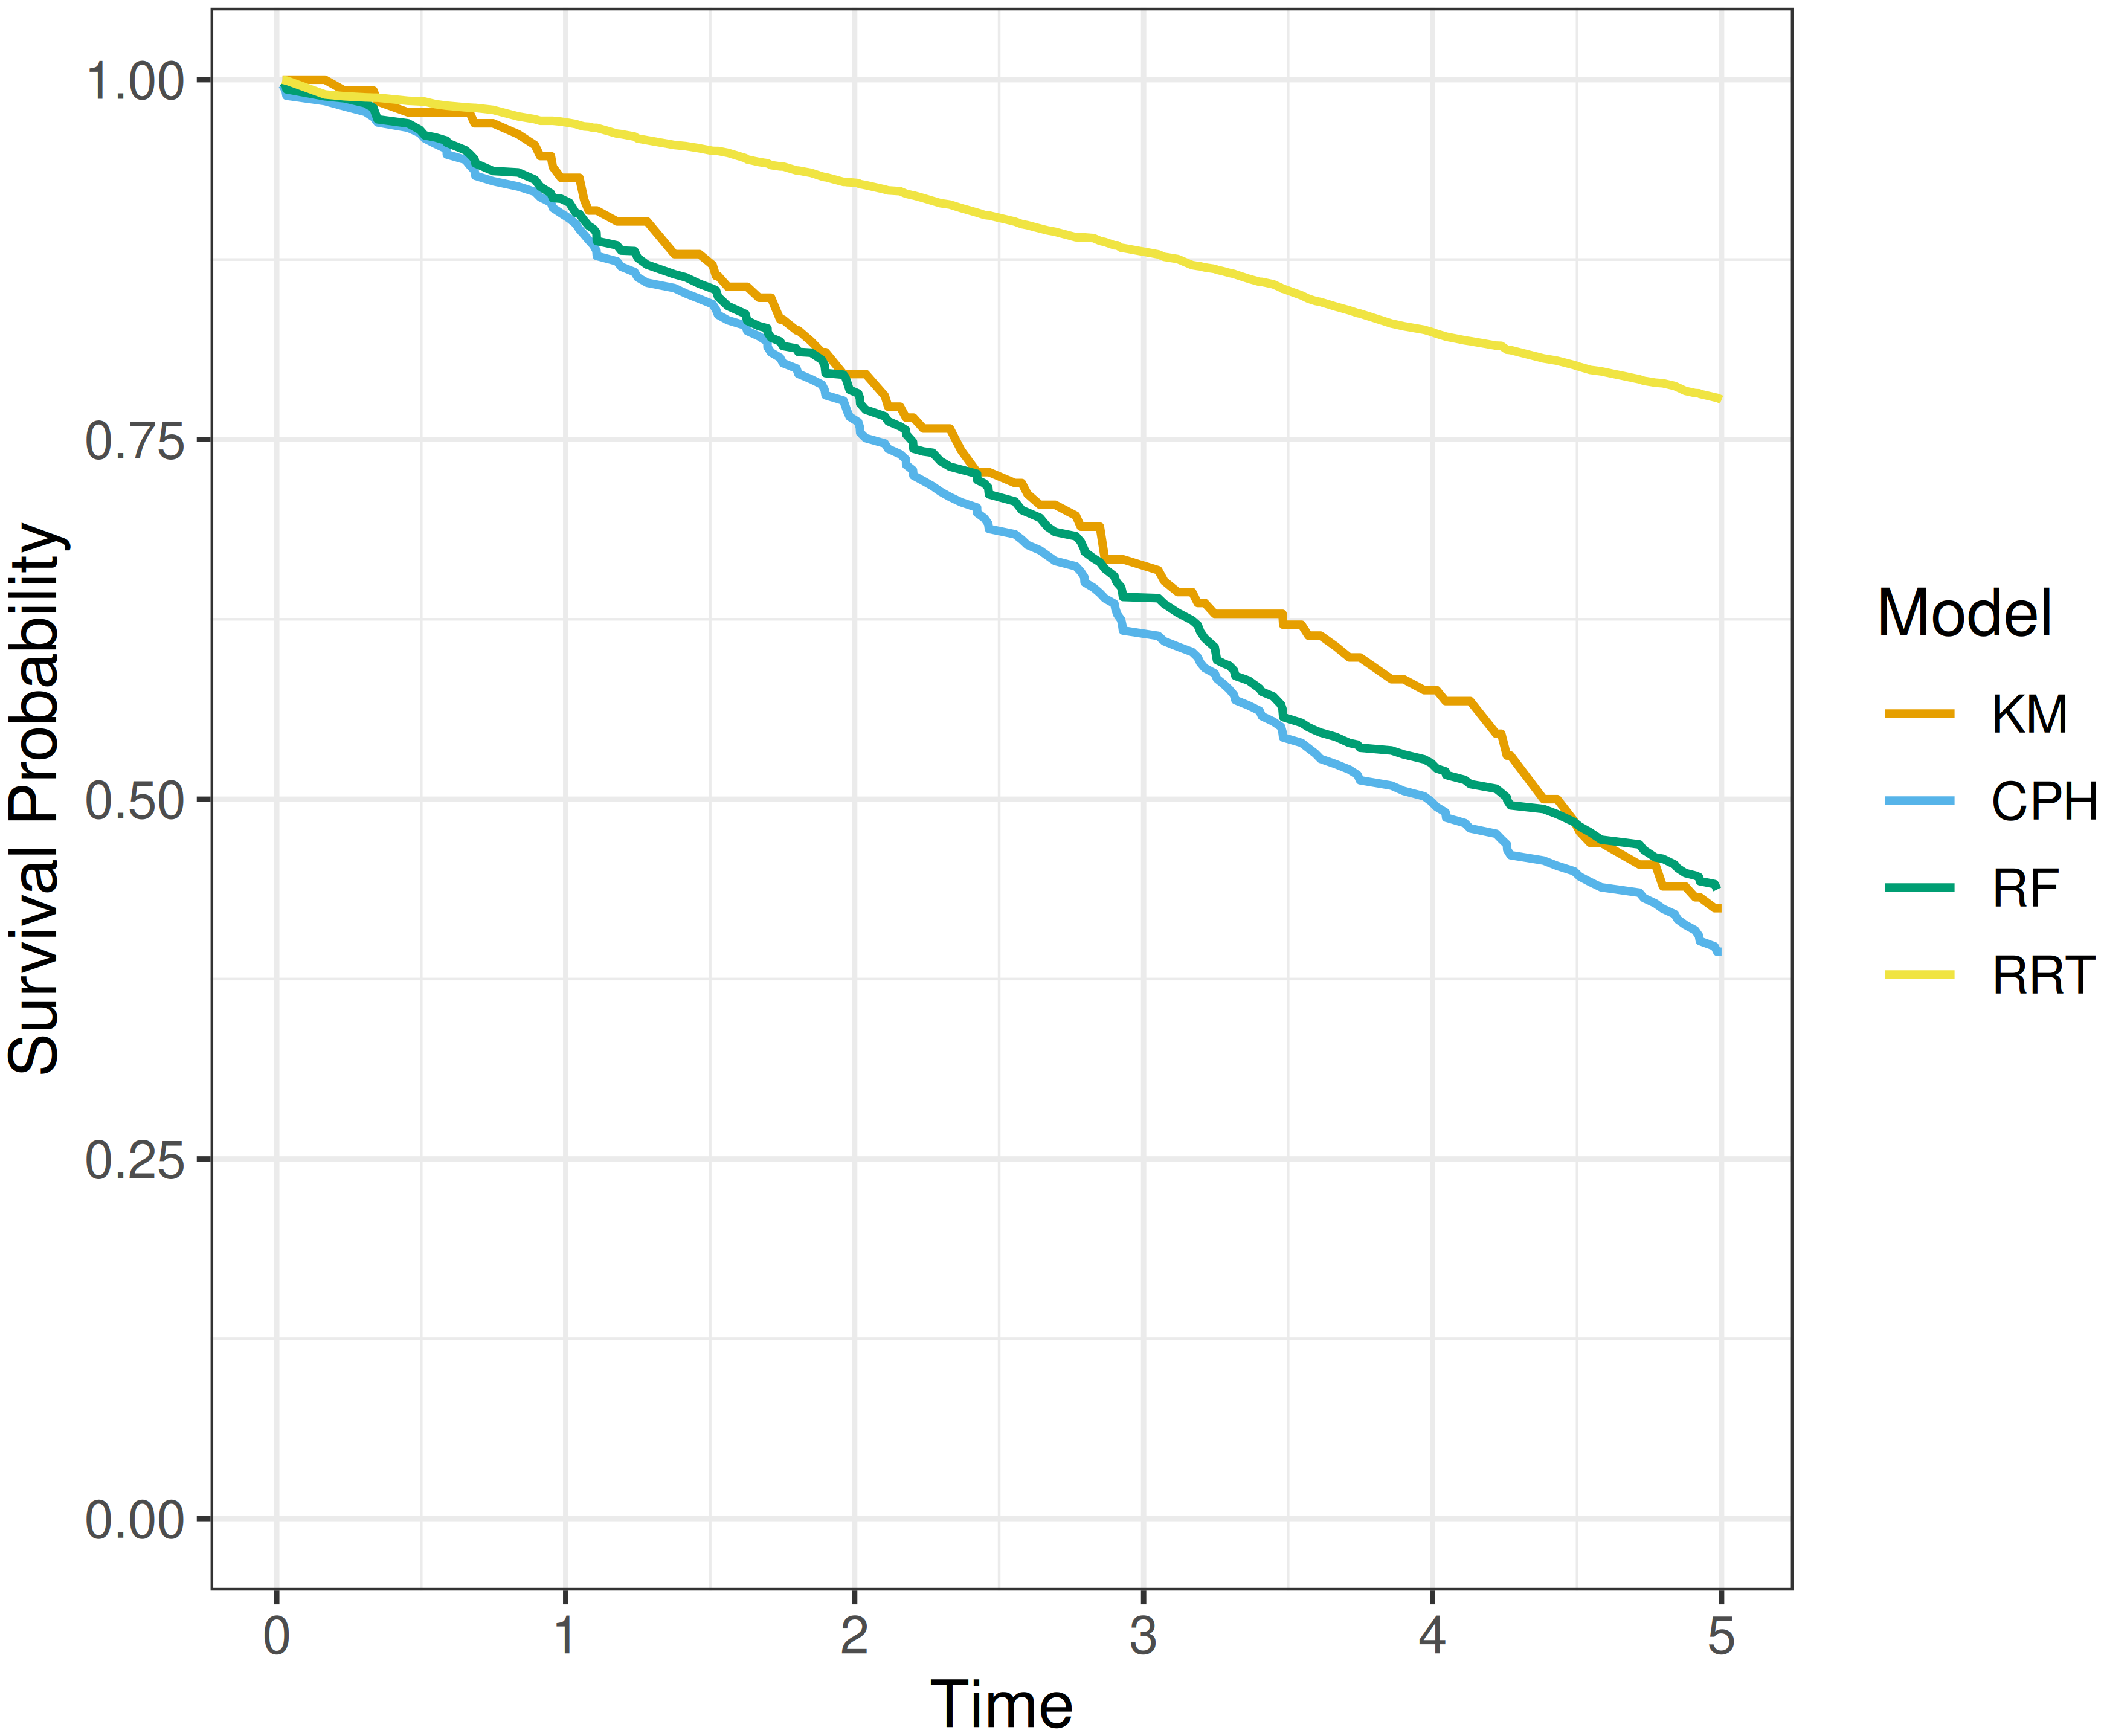
\includegraphics[width=0.7\linewidth,height=\textheight,keepaspectratio]{Figures/evaluation/fig-p2c9-calibKM.png}

}

\caption{\label{fig-p2c9-calibKM}Comparing the calibration of a Cox PH
(CPH), random forest (RF), and relative risk tree (RRT) to the
Kaplan-Meier estimate of the survival function calculated on a test set.
The calibration of RRT notably decreases over time whereas RF and CPH
are closer to the Kaplan-Meier curve.}

\end{figure}%

This method is useful for making broad statements such as ``model X is
clearly better calibrated than model Y'' or ``model X appears to make
average predictions close to the Kaplan-Meier estimate'', but limited
quantitative interpretation is provided. This is also only a marginal
calibration check; it assesses whether the average predicted survival
curve agrees with the average experience across the whole test set and
does not guarantee calibration within meaningful subgroups. This method
can be refined for more fine-grained information by instead using
predictions to create `risk groups' that can be plotted against a
stratified Kaplan-Meier (Peter C. Austin, Harrell Jr, and Klaveren
2020). However, this is harder to interpret and adds subjectivity around
the number of risk groups to create and how they are defined (Peter C.
Austin, Harrell Jr, and Klaveren 2020; Royston and Altman 2013).

As this approach depends on a non-parametric estimator to represent the
ground truth, it can be naturally extended to other censoring and
truncation settings. For example, replacing the Kaplan-Meier estimator
with the non-parametric maximum likelihood estimator
(Section~\ref{sec-surv-estimation-non-param}) enables calibration when
interval censoring is present, or using the left-truncated risk-set
definition (Section~\ref{sec-non-param-lt}) allows application to
left-truncated data.\index{truncation!left} Similarly, this approach can
evaluate competing risks\index{competing risks} data by comparing
predicted cumulative incidence
functions\index{cumulative incidence function} (CIFs) for a particular
event to the CIF estimated with the Aalen-Johansen
estimator\index{Aalen-Johansen estimator}
(Section~\ref{sec-aalen-johansen}) (Peter C. Austin et al. 2022b;
Wolbers et al. 2009). Interpretation becomes challenging in the
competing risks setting as separate plots are required for each cause,
making it difficult to assess calibration over multiple events.

\subsection{D-calibration}\label{sec-dcalib}

Recall that calibration measures assess whether model predictions align
with population-level outcomes.\index{calibration!D-calibration} In
probabilistic classification, this means testing if predicted
probabilities align with observed frequencies. For example, among all
instances where a model predicts a 70\% probability of the event
happening, approximately 70\% of the corresponding observations should
actually experience the event. In survival analysis, calibration is
extended by examining if predicted survival probabilities align with the
actual distribution of event times. This is motivated by a well-known
result: for any continuous random variable \(X\), it holds that
\(S_X(X) \sim \mathcal{U}(0,1)\) (Angus 1994). This means that,
regardless of whether the true outcome times, \(Y\), follow a Weibull,
Gompertz, or any other continuous distribution, the survival
probabilities evaluated at those times should be uniformly distributed
in a well-calibrated model,

\begin{equation}\phantomsection\label{eq-surv-su}{
\hat{S}(Y) \sim \mathcal{U}(0,1).
}\end{equation}

D-calibration (Andres et al. 2018; Haider et al. 2020) leverages the
fact that the event times, \(y_i\), are independent and identically
distributed realizations from the distribution of \(Y\), which justifies
replacing \(Y\) with \(y_i\) in (\ref{eq-surv-su}) (Lemma B.2 Haider et
al. 2020). A survival model is considered well-calibrated if the
predicted survival probabilities at event times follow a standard
uniform distribution: \(\hat{S}(y_i) \sim \mathcal{U}(0,1)\) --- for now
censoring is ignored.

To test whether a random variable follows a particular distribution, in
this case if the predicted survival probabilities follow a standard
uniform distribution\index{uniform distribution}, the \(\chi^2\) test
statistic can be employed:\index{chi-squared@chi-squared, $\chi^2$}

\[
\chi^2 := \sum_{g=1}^G \frac{(o_g - e_g)^2}{e_g}
\]

where \(o_g, e_g\) are respectively the number of observed and expected
event counts in groups \(g = 1,\ldots,G\).

To estimate the expected number of observations, first note that for
this measure the \(\chi^2\) statistic tests whether predicted survival
probabilities are evenly distributed across the \([0,1]\) interval. To
do so, the \([0,1]\) range is partitioned into \(G\) equal-width bins.
If \(n\) is the total number of observations, then under the null
hypothesis of a uniform distribution, the expected number of events in
each bin is \(e_g = n/G\).

To define the observed number of events in the \(g\)th bin,
\(\mathcal{B}_g\), first define the bin as the set:

\[
\mathcal{B}_g := \{i = 1,\ldots,n : \lceil \hat{S}(y_i \mid \mathbf{x}_i) \times G \rceil = g\}
\]

where \(i = 1,\ldots,n\) are the indices of the observations,
\(\hat{S}(\cdot \mid \mathbf{x}_i)\) are predicted survival functions,
\(y_i\) are observed event times, and \(\lceil \cdot \rceil\) is the
ceiling function. To avoid edge-case issues, the algorithm sets the
predicted survival probability such that
\(\hat{S}(t_i \mid \mathbf{x}_i) = 0\) is replaced with
\(1\times10^{-5}\). For example, say there are \(5\) bins:
\(\{[0, 0.2], (0.2, 0.4], (0.4, 0.6], (0.6, 0.8], (0.8, 1]\}\). The
predicted survival probability for observation \(i\) is
\(\hat{S}(y_i \mid \mathbf{x}_i) = 0.7\). Then, observation \(i\) falls
into the fourth bin:
\(\lceil 0.7 \times 5 \rceil = \lceil 3.5 \rceil = 4\).

The observed number of events can now be defined simply as the number of
observations in the corresponding set:
\(o_g = \vert \mathcal{B}_g \vert\).

Extension to all observed outcomes, \(t_i\), follows by partially
allocating censored observations across multiple bins according to their
conditional probability of belonging to each bin (Algorithm 2, Haider et
al. (2020)); conditional event-independent censoring is assumed.

The D-calibration measure, based on the \(\chi^2\) statistic, is then
defined by:

\[
D_{\chi^2}(\hat{\mathbf{S}}, \mathbf{t}) :=  \frac{\sum^G_{g = 1} (o_g - \frac{n}{G})^2}{n/G}
\]

where \(\hat{\mathbf{S}}\) is the vector of predicted survival functions
and \(\boldsymbol{\mathbf{t}} = ({t}_1 \ {t}_2 \cdots {t}_{n})^\top\)
are the observed outcomes.

This measure has several useful properties. Firstly, the measure
provides a simple quantitative summary through the test statistic and
can be used to test the hypothesis that a model is `D-calibrated' since,
under the null, \(D_{\chi^2}\) asymptotically follows a \(\chi^2_{G-1}\)
distribution, from which a \(p\)-value can be obtained. Secondly,
\(D_{\chi^2}\) tends to zero as a model is increasingly well-calibrated,
hence the measure can be used for model comparison. Finally, the theory
lends itself to an intuitive graphical calibration
method\index{calibration!plots}. A D-calibrated model implies

\begin{equation}\phantomsection\label{eq-dcalib-quant}{
p \approx \frac{\sum_i \mathbb{I}(t_i \leq \hat{F}_i^{-1}(p))}{n},
}\end{equation}

where \(p\) is some value in \([0,1]\), \(\hat{F}_i^{-1}\) is the
\(i\)th predicted inverse cumulative distribution function, and \(n\) is
the number of observations. In words, the proportion of events occurring
at or before each prediction \(p\)-quantile should equal \(p\) itself,
for example 50\% of events should occur before their predicted median
survival time. By plotting \(p\) on the x-axis and the right-hand side
of (\ref{eq-dcalib-quant}) on the y-axis, a perfectly D-calibrated model
results in a straight line on \(x = y\). This is visualized in
Figure~\ref{fig-p2c9-calibD} for the same models as in
Figure~\ref{fig-p2c9-calibKM}. This figure supports the previous
findings that the relative risk tree is poorly calibrated in contrast to
the Cox PH and random forest but again direct comparison between the
latter models is difficult from visual inspection alone.

While D-calibration shares the same limitations as Kaplan-Meier
calibration plots for visual comparison, it additionally provides
quantitative summaries that support more concrete conclusions. Returning
to Figure~\ref{fig-p2c9-calibD}, the relative risk tree is confirmed to
be poorly D-calibrated with \(p<0.01\), indicating that the null
hypothesis, that predicted survival probabilities follow the standard
uniform distribution, can be rejected. Although the D-calibration
statistics for the Cox PH and random forest differ slightly, the
difference does not appear significant, as reflected in the overlapping
curves.

\begin{figure}

\centering{

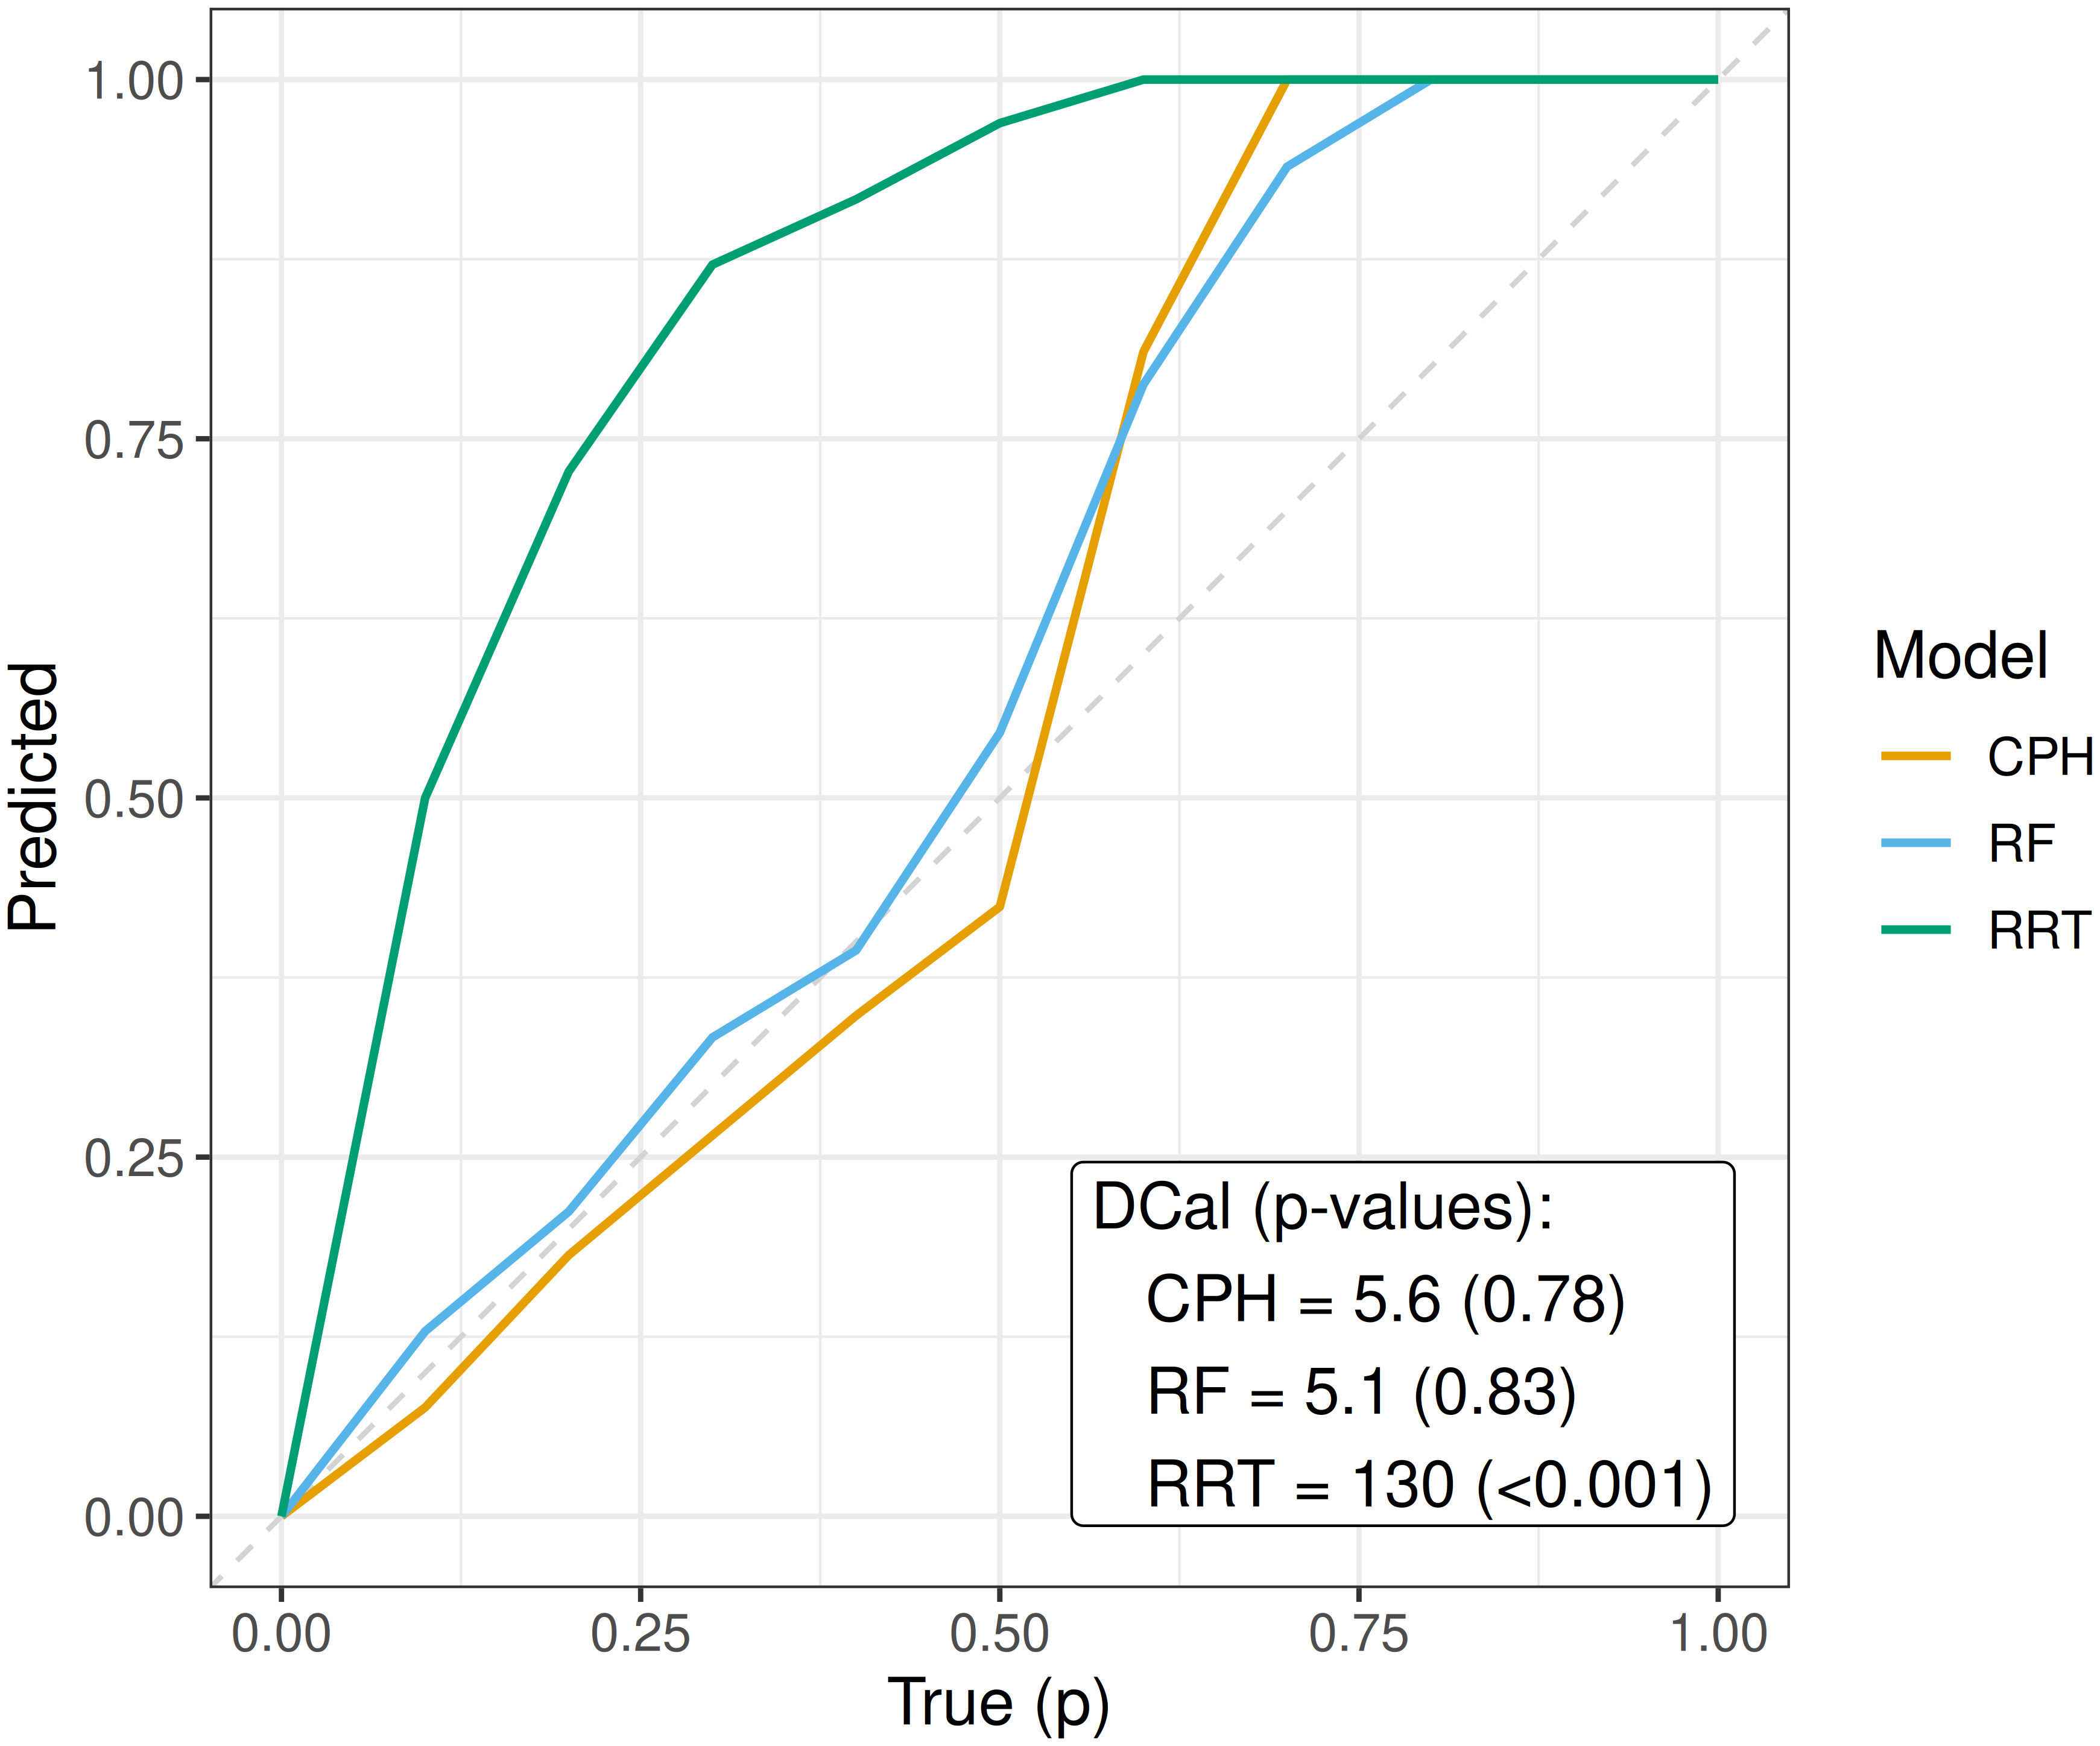
\includegraphics[width=0.7\linewidth,height=\textheight,keepaspectratio]{Figures/evaluation/fig-p2c9-calibD.png}

}

\caption{\label{fig-p2c9-calibD}Comparing the D-calibration of a Cox PH
(CPH), random forest (RF), and relative risk tree (RRT) to the expected
distribution on y=x. As with Figure~\ref{fig-p2c9-calibKM}, the relative
risk tree is clearly not D-calibrated (as supported by the \(p\)-values
in the bottom-right). The CPH and RF are closer to the y=x line;
however, neither follows it perfectly.}

\end{figure}%

\section{Conclusion}\label{conclusion-5}

\begin{tcolorbox}[enhanced jigsaw, toprule=.15mm, bottomtitle=1mm, opacityback=0, breakable, leftrule=.75mm, title={Key takeaways}, toptitle=1mm, bottomrule=.15mm, colback=white, colframe=quarto-callout-warning-color-frame, titlerule=0mm, opacitybacktitle=0.6, coltitle=black, rightrule=.15mm, left=2mm, colbacktitle=quarto-callout-warning-color!10!white, arc=.35mm]

\begin{itemize}
\tightlist
\item
  Calibration measures assess the population-level agreement between
  predicted survival distributions and observed outcomes. By definition,
  good calibration does not imply good individual-level predictions. A
  model can be well calibrated on average while still having poor
  discrimination, so calibration measures should not be interpreted in
  isolation from other performance metrics.
\item
  Graphical approaches provide an intuitive method to assess model
  calibration qualitatively. Moreover, as they often depend on
  non-parametric estimators, it is possible to incorporate different
  censoring and truncation mechanisms. Graphical comparisons alone do
  not support formal statistical comparison between models and can
  become difficult to interpret when multiple outcomes or competing
  risks are present.
\item
  Event frequency calibration evaluates if the total number of observed
  and predicted events are roughly equal. This method is particularly
  informative when interpreted alongside scoring rules
  (Chapter~\ref{sec-rules}), which capture both calibration and
  discrimination.
\item
  D-calibration assesses calibration over the entire predicted
  distribution by testing if predicted survival probabilities at
  observed event times follow a uniform distribution. This method also
  supports interpretable graphical plots for qualitative assessment.
\item
  Some numerical methods for calibration in a competing risk setting
  have been proposed (Schoop, Schumacher, and Graf 2011; Geloven et al.
  2022). These can be complex to implement and interpret and graphical
  methods appear more often used in practice (Monterrubio-Gómez,
  Constantine-Cooke, and Vallejos 2024).
\end{itemize}

\end{tcolorbox}

\begin{tcolorbox}[enhanced jigsaw, toprule=.15mm, bottomtitle=1mm, opacityback=0, breakable, leftrule=.75mm, title={Further reading}, toptitle=1mm, bottomrule=.15mm, colback=white, colframe=quarto-callout-tip-color-frame, titlerule=0mm, opacitybacktitle=0.6, coltitle=black, rightrule=.15mm, left=2mm, colbacktitle=quarto-callout-tip-color!10!white, arc=.35mm]

\begin{itemize}
\tightlist
\item
  A calibration measure based on the Akritas goodness-of-fit-test was
  recently introduced in Simonsen and Waagepetersen (2025).
\item
  For calibration measures specifically focused on re-calibrating Cox PH
  models, see Peter C. Austin, Harrell Jr, and Klaveren (2020), Demler,
  Paynter, and Cook (2015), and Van Houwelingen (2000).
\item
  Haider et al. (2020) review further calibration measures and suggest
  algorithms for estimating the Hosmer-Lemeshow test in a survival
  analysis setting.
\end{itemize}

\end{tcolorbox}

\chapter{Scoring Rules}\label{sec-rules}

Scoring rules\index{scoring rules} evaluate probabilistic predictions
and measure the overall predictive ability of a model, capturing aspects
of both calibration\index{calibration} and
discrimination\index{discrimination} (Gneiting and Raftery 2007; Murphy
1973). In contrast to calibration measures, which assess the average
agreement between predicted and observed outcomes at a \emph{population}
level, scoring rules evaluate the sample mean of \emph{individual}
losses across all observations in a test set. Scoring rules are
increasingly popular as probabilistic forecasts are widely recognized to
be superior to deterministic predictions for capturing uncertainty in
predictions (A. P. Dawid 1984; A. Philip Dawid 1986). The formalization
and development of scoring rules has primarily been due to Dawid (A. P.
Dawid 1984; A. Philip Dawid 1986; Alexander Philip Dawid and Musio 2014)
and Gneiting and Raftery (Gneiting and Raftery 2007), though the
earliest measures promoting ``rational'' and ``honest'' decision making
date back to the 1950s (Brier 1950; Good 1952). While few scoring rules
have been proposed in survival analysis, there has been a notable
increase in research into this area over the past few years. Before
delving into these measures, this section begins by first describing
scoring rules in the simpler classification
setting.\index{Brier score}\index{log loss}

Note that in the literature there is ambiguity around the definitions of
scoring rule, loss, and score. Here, a \emph{scoring rule} is a term for
a function that takes as inputs a probabilistic prediction and an
observed outcome and may have the properties: properness and strict
properness (introduced below). In some literature, the terms \emph{loss}
and \emph{score} are used to distinguish whether the scoring rule is
optimized by minimization or maximization. To avoid confusion, each
scoring rule below is described in terms of whether lower or higher
values indicate better predictive performance.

Scoring rules are pointwise losses, meaning a loss is calculated for all
observations and the sample mean is then calculated over all losses.
Each scoring rule is therefore introduced for a single observation \(i\)
only. To simplify notation, let \(\hat{S}_i\) be a shorthand for the
survival function prediction for observation \(i\), usually written as
\(\hat{S}(\cdot \mid \mathbf{x}_i)\); analogously for other
distribution-defining functions. As distribution-defining functions can
be derived from one another
(Section~\ref{sec-distributions-continuous}), only one function is
included in the signature for losses. As usual, \((t_i, \delta_i)\) is
the observed survival outcome.

\section{Classification losses}\label{classification-losses}

In the simplest terms, a scoring rule compares a probabilistic
prediction to an observed outcome and assigns them a scalar value, the
loss. Formally, a loss function is written as

\[
L: \mathcal{P}\times \mathcal{Y}\to \bar{\mathbb{R}},
\]

where \(p \in \mathcal{P}\) is a (predicted) probability distribution
over the outcome space \(\mathcal{Y}\); for classification tasks,
\(\mathcal{Y}\subseteq \mathbb{N}_0\), and for binary classification,
\(\mathcal{Y}= \{0,1\}\).

As an example, take the Brier score for binary
classification\index{classification!binary} (Brier 1950) defined
by:\index{Brier score} \begin{equation}\phantomsection\label{eq-brier}{
L_{Brier}(\hat{p}_i, y_i) = (y_i - \hat{p}_i)^2,
}\end{equation}

where \(\hat{p}_i \equiv \hat{p}_i(y_i = 1)\) is the predicted
probability of the positive class, or in survival terms the event of
interest, and \(y_i \in \{0,1\}\) is the ground truth.

This loss is minimized when the predicted probability matches the
observed outcome: \(\hat{p}_i(y_i = 1) = y_i\). If the event occurs then
\(y_i = 1\) and the optimal prediction is \(\hat{p}_i(y_i = 1) = 1\);
otherwise if the event does not occur then \(y_i = 0\) and the optimal
prediction is \(\hat{p}_i(y_i = 1) = 0\).

This motivates an important property of scoring rules,
\emph{properness}.\index{scoring rules!proper} A loss is \emph{proper}
if it is minimized in expectation by the true prediction. In contrast,
if \(L_{improper}(\hat{p}_i, y_i) = 1 - L_{Brier}(\hat{p}_i, y_i)\) were
treated as a loss to be minimized, then it is an \emph{improper} scoring
rule as perfect predictions result in a loss value of \(1\) whereas the
worst predictions result in a value of \(0\). Proper losses provide a
method of model comparison as, by definition, predictions closest to the
true distribution will result in lower expected losses.

Another important property is \emph{strict}
properness.\index{scoring rules!strictly proper} A loss is
\emph{strictly proper} if the loss is uniquely minimized by the correct
prediction. For example, the expected Brier score for a binary outcome
is uniquely minimized when the predicted probability equals the true
event probability (Figure~\ref{fig-p2c10-brier-logloss}). Strictly
proper losses are particularly important for automated model
optimization, as minimization of the loss will result in the ``optimum
score estimator based on the scoring rule'' (Gneiting and Raftery 2007).

Formally, for any distributions \(p_Y, p \in \cal P\) and for any random
variables \(Y \sim p_Y\), a classification loss
\(L: \mathcal{P}\times \mathcal{Y}\rightarrow \bar{\mathbb{R}}\) is
called:

\begin{itemize}
\tightlist
\item
  \emph{proper} if
  \(\mathbb{E}_Y[L(p_Y, Y)] \leq \mathbb{E}_Y[L(p, Y)]\) for all
  \(p \in \mathcal{P}\);
\item
  \emph{strictly proper} if in addition to being proper,
  \(\mathbb{E}_Y[L(p_Y, Y)] = \mathbb{E}_Y[L(p, Y)]\) if and only if
  \(p = p_Y\).
\end{itemize}

In addition to the Brier score (\ref{eq-brier}), another widely used
strictly proper loss (Alexander Philip Dawid and Musio 2014) is the log
loss (Good 1952), defined by\index{log loss}

\begin{equation}\phantomsection\label{eq-logloss}{
L_{logloss}(\hat{p}_i, y_i) = -\log \hat{p}_i(y_i),
}\end{equation}

where again \(y_i \in \{0,1\}\) is the ground truth and \(\hat{p}_i\) is
a predicted probability distribution. The log loss is minimized at \(0\)
but is unbounded above.

These losses are visualized in Figure~\ref{fig-p2c10-brier-logloss};
both approach their minima as predicted probabilities come closer to the
observed outcome. It can also be seen from the scale of the plots that
the log loss penalizes wrong predictions more strongly than the Brier
score, which may be beneficial or not depending on the given use case.

\begin{figure}

\centering{

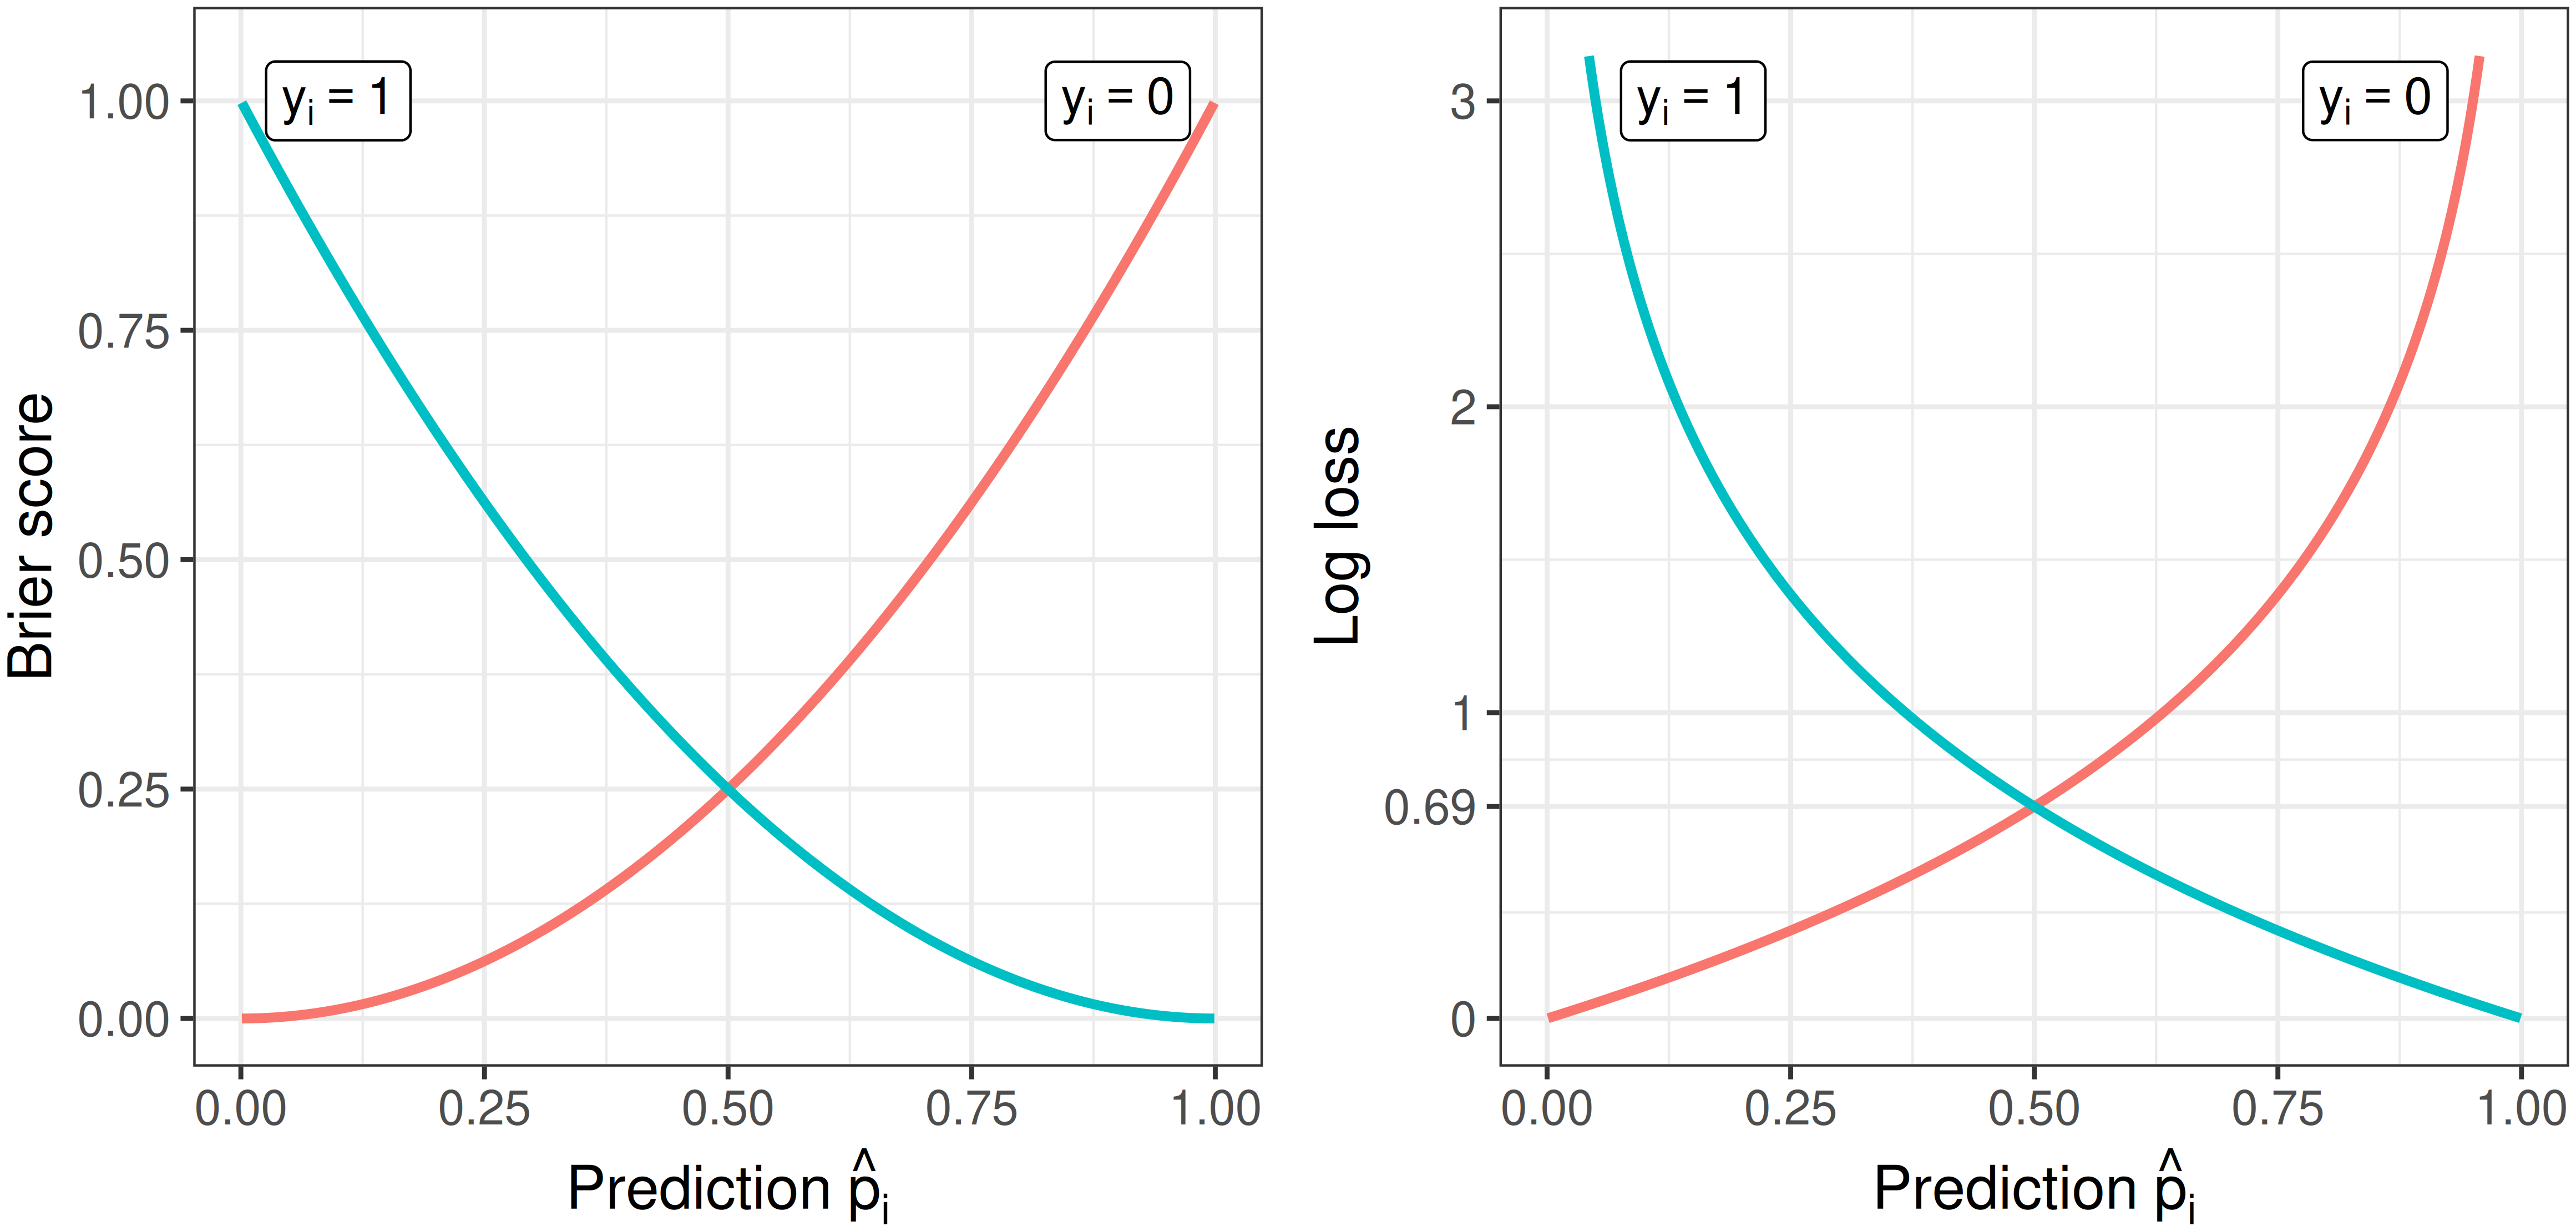
\includegraphics[width=0.9\linewidth,height=\textheight,keepaspectratio]{Figures/evaluation/fig-p2c10-brier-logloss.png}

}

\caption{\label{fig-p2c10-brier-logloss}Brier and log loss scoring rules
for a binary outcome and varying probabilistic predictions. x-axis is a
probabilistic prediction in \([0,1]\), y-axis is Brier score (left) and
log loss (right). Blue lines are varying Brier score/log loss over
different predicted probabilities when the true outcome is 1. Red lines
are varying Brier score/log loss over different predicted probabilities
when the true outcome is 0. Both losses are minimized when the predicted
probability matches the observed outcome.}

\end{figure}%

\section{Survival losses}\label{sec-eval-distr-commonsurv}

Analogously to classification losses, one can define a survival loss
as\index{survival loss}

\[
L_S: \mathcal{P}\times \mathcal{T}\times \{0,1\}\rightarrow \bar{\mathbb{R}},
\]

where now \(\mathcal{P}\) denotes a set of probability distributions
over \(\mathbb{R}_{>0}\) and \(\mathcal{T}\subseteq \mathbb{R}_{>0}\).
This formulation assumes right-censoring only but analogous definitions
can be formulated for event history analysis.

For any distributions \(p_Y, p\) in \(\mathcal{P}\) and for any random
variables \(Y \sim p_Y\) and a censoring variable \(C\), with
\(T := \min\{Y,C\}\) and \(\Delta := \mathbb{I}(Y \le C)\), then a
survival loss \(L_S\) is called:

\begin{itemize}
\tightlist
\item
  \emph{proper} if
  \(\mathbb{E}_{T, \Delta} [L_S(p_Y, T, \Delta)] \le \mathbb{E}_{T,\Delta}[L_S(p, T, \Delta)]\)
  for all \(p \in \mathcal{P}\);
\item
  \emph{strictly proper} if in addition to being proper,
  \(\mathbb{E}_{T, \Delta} [L_S(p_Y, T, \Delta)] = \mathbb{E}_{T,\Delta}[L_S(p, T, \Delta)]\)
  if and only if \(p = p_Y\).
\end{itemize}

With these definitions, the rest of this chapter lists common scoring
rules in survival analysis and discusses some of their properties. As
with other chapters, this list is not exhaustive but will cover commonly
used losses. The losses are grouped into squared losses, absolute
losses, and logarithmic losses, which respectively estimate the mean
squared error\index{mean squared error}, mean absolute
error\index{mean absolute error}, and log loss\index{log loss} in
uncensored settings.

\begin{tcolorbox}[enhanced jigsaw, toprule=.15mm, bottomtitle=1mm, opacityback=0, breakable, leftrule=.75mm, title={Box 3 (Estimating censoring distributions for IPCW)}, toptitle=1mm, bottomrule=.15mm, colback=white, colframe=quarto-callout-note-color-frame, titlerule=0mm, opacitybacktitle=0.6, coltitle=black, rightrule=.15mm, left=2mm, colbacktitle=quarto-callout-note-color!10!white, arc=.35mm]

Inverse probability of censoring weighting
(IPCW)\index{inverse probability of censoring weights} is used to
account for removal of censored observations
(Section~\ref{sec-surv-ipcw}). For discrimination measures
(Chapter~\ref{sec-eval-crank}), there appears to be broad consensus
around weighting schemes based on non-parametric estimators, namely the
Kaplan-Meier estimator.\index{Kaplan-Meier estimator} For scoring rules,
there is less consensus about how the censoring distribution should be
estimated. Common approaches include:\index{censoring distribution}

\begin{enumerate}
\def\labelenumi{\arabic{enumi}.}
\tightlist
\item
  Non-parametric estimators: For example, the Kaplan-Meier estimator may
  be used to estimate the marginal censoring distribution. This is
  likely the oldest and most commonly used approach and assumes
  censoring is marginally independent of the event time;
\item
  Fitted models: A secondary survival model, such as the Cox PH, is
  fitted to the censoring distribution. This may account for censoring
  that is conditionally independent of the event time;
\item
  Joint or iterative estimation: A censoring model is estimated
  alongside the event model, most commonly in approaches such as
  boosting\index{gradient boosting machines} (Chapter~\ref{sec-boost})
  and neural networks\index{neural networks} (Chapter~\ref{sec-nnet}).
  This allows flexible censoring models but introduces additional
  modeling assumptions.
\end{enumerate}

The non-parametric approach is simple and widely used, but may lead to
biased estimators when censoring depends on covariates (Thomas A. Gerds
and Schumacher 2006). Model-based estimates may account for such
censoring mechanisms, but their validity depends on assumptions about
the censoring model. In practice, these models are typically assumed to
be correctly specified rather than externally validated. When this
assumption is violated and the censoring model is misspecified, bias may
be introduced into the resulting measure. This creates an additional
modeling problem, as the validity of IPCW depends on assumptions about
the censoring distribution.

In predictive settings, the ranks induced by losses are often more
important than their absolute values. In such settings, (strict)
properness may be more relevant for model comparison and optimization
than consistency guarantees. In practice, software implementations often
allow flexibility in how the censoring distribution is estimated, and
the relative merits of these approaches are not discussed further here.

Throughout this chapter, \(\hat{G}(\cdot)\) denotes an estimate of the
censoring survival distribution, whether obtained non-parametrically or
via a fitted model.

\end{tcolorbox}

\subsection{Squared losses}\label{sec-rules-squared}

The integrated survival Brier
score\index{integrated survival Brier score} was introduced by Graf
(Graf and Schumacher 1995; Graf et al. 1999) as an analogue to the
integrated Brier score in regression. It is likely the most commonly
used scoring rule in survival analysis, possibly due to its intuitive
interpretation.

At a single time point, the survival Brier score (SBS) is given by,

\begin{equation}\phantomsection\label{eq-sbs}{
L_{SBS}(\tau, \hat{S}_i, t_i, \delta_i \mid \hat{G}) = \frac{\hat{S}_i^2(\tau) \mathbb{I}(t_i \leq \tau, \delta_i=1)}{\hat{G}(t_i)} + \frac{\hat{F}_i^2(\tau) \mathbb{I}(t_i > \tau)}{\hat{G}(\tau)},
}\end{equation}

where \(\hat{S}_i^2(\tau) = (\hat{S}_i(\tau))^2\) and
\(\hat{F}_i^2(\tau) = (1 - \hat{S}_i(\tau))^2\), and \(\hat{G}\) is the
estimated censoring survival function used for IPC weighting (Box 3).

At first glance this might seem intimidating but it is worth taking the
time to understand the intuition behind the loss. Recall the
classification Brier score (\ref{eq-brier}), which provides a method to
evaluate a probability mass function at a single point. In a regression
setting, the \emph{integrated Brier
score}\index{integrated Brier score}, also known as the continuous
ranked probability score, is the integral of the Brier score for all
real-valued thresholds (Gneiting and Raftery 2007) and hence allows
predictions to be evaluated over multiple points as:

\begin{equation}\phantomsection\label{eq-crps}{
L(\hat{F}_i, y_i) = \int (\mathbb{I}(y_i \leq \tau) - \hat{F}_i(\tau))^2 \,\mathrm{d}\tau,
}\end{equation}

where \(\hat{F}_i\) is the predicted cumulative distribution function
and \(\tau\) is some meaningful threshold. As the indicator in
(\ref{eq-crps}) can only take one of two values, the integrand of
(\ref{eq-crps}) can be represented as two distinct cases, now using
\(t_i\) instead of \(y_i\) to represent time:

\[
(\mathbb{I}(t_i \leq \tau) - \hat{F}_i(\tau))^2 =
\begin{cases}
(1 - \hat{F}_i(\tau))^2 = \hat{S}_i^2(\tau), & \text{ if } t_i \leq \tau, \\
(0 - \hat{F}_i(\tau))^2 = \hat{F}_i^2(\tau), & \text{ if } t_i > \tau.
\end{cases}
\]

In the first case, the observation experienced the event before
\(\tau\), hence the optimal prediction for \(\hat{F}_i(\tau)\) (the
probability of experiencing the event before \(\tau\)) is \(1\), and
therefore the optimal \(\hat{S}_i(\tau)\) is \(0\). Conversely, in the
second case where the observation has not experienced the event, the
optimal \(\hat{F}_i(\tau)\) is \(0\). The loss therefore meaningfully
represents the ideal predictions in the two possible real-world
scenarios.

To accommodate censoring, note that at \(\tau\) an observation will
either have:

\begin{enumerate}
\def\labelenumi{\arabic{enumi}.}
\tightlist
\item
  not yet experienced the event or censoring: \(t_i > \tau\);
\item
  experienced the event: \(t_i \leq \tau \wedge \delta_i = 1\); or
\item
  been censored: \(t_i \leq \tau \wedge \delta_i = 0\).
\end{enumerate}

Censored observations are discarded after the censoring time as
evaluating predictions after this time is impossible as the ground truth
is unknown. To compensate for removing observations,
IPCW\index{inverse probability of censoring weights} (Box 3) is again
used to upweight predictions as \(\tau\) increases. IPC weights are
defined such that observations are either weighted by
\(\hat{G}^{-1}(\tau)\) when they have not yet experienced the event or
by their final observed time, \(\hat{G}^{-1}(t_i)\), otherwise
(Table~\ref{tbl-ipcw-weights}).

\begin{longtable}[]{@{}lll@{}}
\caption{IPC weighting scheme for the
ISBS.}\label{tbl-ipcw-weights}\tabularnewline
\toprule\noalign{}
& \(t_i > \tau\) & \(t_i \leq \tau\) \\
\midrule\noalign{}
\endfirsthead
\toprule\noalign{}
& \(t_i > \tau\) & \(t_i \leq \tau\) \\
\midrule\noalign{}
\endhead
\bottomrule\noalign{}
\endlastfoot
\(\delta_i = 1\) & \(\hat{G}^{-1}(\tau)\) & \(\hat{G}^{-1}(t_i)\) \\
\(\delta_i = 0\) & \(\hat{G}^{-1}(\tau)\) & \(0\) \\
\end{longtable}

Finally, to obtain a scalar summary of predictive ability over a time
horizon, (\ref{eq-sbs}) can be integrated to give the integrated
survival Brier score (ISBS),

\begin{equation}\phantomsection\label{eq-igs}{
L_{ISBS}(\tau^*, \hat{S}_i, t_i, \delta_i \mid \hat{G}) = \int^{\tau^*}_0  \frac{\hat{S}_i^2(\tau) \mathbb{I}(t_i \leq \tau, \delta_i=1)}{\hat{G}(t_i)} + \frac{\hat{F}_i^2(\tau) \mathbb{I}(t_i > \tau)}{\hat{G}(\tau)} \,\mathrm{d}\tau,
}\end{equation}

where \(\tau^* \in \mathbb{R}_{>0}\) is an upper threshold to compute
the loss up to. As with the cutoff in concordance measures, a common
rule of thumb is to set \(\tau^*\) to be the time point at which 80\% of
the observations have experienced the event or censoring
(Section~\ref{sec-eval-crank-choose}).

When censoring is marginally independent, the ISBS consistently
estimates the mean squared error\index{mean squared error} (Thomas A.
Gerds and Schumacher 2006). However, the SBS and ISBS are only proper
under strict conditions: marginally independent censoring and no Type I
censoring; under other conditions the losses are improper (Rindt et al.
2022; Sonabend et al. 2025). Despite this, the loss is deeply embedded
in the survival literature and early research indicates that with a
suitable choice of \(\tau^*\), even when censoring is only conditionally
independent, the loss behaves approximately as a proper loss in practice
(Sonabend et al. 2025).

There has been limited work in extending squared losses to handle other
forms of censoring and truncation, though one notable extension is an
adaptation of the ISBS for administrative censoring (Kvamme and Borgan
2023). There is some sparse research into extending the ISBS to handle
interval censoring by estimating the probability of survival within the
interval (Tsouprou 2015), however there appears to be little evidence of
use in practice.

\subsection{Logarithmic losses}\label{sec-rules-log}

The development of logarithmic losses follows from adapting the negative
log-likelihood for censored datasets. Consider the usual negative
log-likelihood in a regression setting, which is a standard measure for
evaluating a model's performance:\index{negative log-likelihood}

\[
L_{NLL}(\hat{f}_i, y_i) = -\log[\hat{f}_i(y_i)],
\]

for a predicted density function \(\hat{f}_i\) and true outcome \(y_i\).
Note this is analogous to the classification log loss in
(\ref{eq-logloss}) with the probability mass function replaced with the
density function.

Now recall (\ref{eq-objective-function}) from
Section~\ref{sec-surv-estimation-param}, which gives the contribution
from a single observation as:

\[
\mathcal{L}_i(\boldsymbol{\theta}) \propto
\begin{cases}
f(t_i \mid \boldsymbol{\theta}), & \text{ if $i$ is uncensored }, \\
S(t_i \mid \boldsymbol{\theta}), & \text{ if $i$ is right-censored }, \\
F(t_i \mid \boldsymbol{\theta}), & \text{ if $i$ is left-censored }, \\
S(l_i \mid \boldsymbol{\theta}) - S(r_i \mid \boldsymbol{\theta}), & \text{ if $i$ is interval-censored }, \\
\end{cases}
\]

where \(r_i, l_i\) are the boundaries of the censoring interval and
\(\boldsymbol{\theta}\) are model parameters (adaptations in the
presence of left-truncation as described in
Section~\ref{sec-surv-estimation-param} may also be applied).

The log loss can then be constructed depending on the type of censoring
or truncation present in the data. For example, if only right-censoring
is present then the right-censored log loss (RCLL) is defined
as:\index{right-censored log loss}

\begin{equation}\phantomsection\label{eq-rcll}{
L_{RCLL}(\hat{S}_i, t_i, \delta_i) = -\log\left(\delta_i\hat{f}_i(t_i) + (1-\delta_i)\hat{S}_i(t_i)\right),
}\end{equation}

where \(\hat{f}_i\) is derived from \(\hat{S}_i\)
(Section~\ref{sec-distributions-continuous}).

If censoring is conditionally independent of the event
(Section~\ref{sec-types-of-censoring}), then this scoring rule is
strictly proper (Yanagisawa 2023). The loss is also interpretable as a
measure of predictive performance when decomposed into two components:

\begin{enumerate}
\def\labelenumi{\arabic{enumi}.}
\tightlist
\item
  An observation censored at \(t_i\) has not experienced the event and
  hence the ideal prediction would be close to \(\hat{S}_i(t_i) = 1\);
  correspondingly (\ref{eq-rcll}) means the loss is minimized for
  censored observations at \(-\log(1) = 0\).
\item
  If an observation experiences the event at \(t_i\), then the loss
  rewards assigning high density near \(t_i\). As \(\hat{f}_i(t_i)\)
  increases, the RCLL contribution decreases and tends to \(-\infty\).
\end{enumerate}

While censored observations contribute non-negative losses only, for
uncensored observations the loss is unbounded below in continuous time.
This means uncensored observations can theoretically contribute more
extreme loss values than censored ones. In practice, many survival
models predict \(\hat{S}_i \in [0,1]\), from which \(\hat{f}_i\) is
numerically derived (Section~\ref{sec-distributions-continuous},
Table~\ref{tbl-dist-transformations}). Under these approximations,
density estimates more frequently lie in \([0,1]\), making strongly
negative losses uncommon.

Other logarithmic losses have also been proposed, such as the integrated
survival log loss (ISLL)\index{integrated survival log loss} in Graf et
al. (1999). The ISLL is similar to the ISBS except \(\hat{S}_i^2\) and
\(\hat{F}_i^2\) are replaced with \(-\log(\hat{S}_i)\) and
\(-\log(\hat{F}_i)\) respectively. The ISLL does not appear to be widely
used in the literature, though the all-cause log loss discussed in
Section~\ref{sec-rules-ext} uses a related formulation.

\subsection{Absolute losses}\label{absolute-losses}

The final class of losses considered here can be viewed as analogs of
the mean absolute error in an uncensored setting. The integrated
survival absolute score
(ISAS)\index{integrated survival absolute score}, developed over time by
Schemper and Henderson (2000) and Schmid et al. (2011), is similar to
the ISBS but removes the squared term:

\[
L_{ISAS}(\tau^*, \hat{S}_i, t_i, \delta_i \mid \hat{G}) = \int^{\tau^*}_0 \frac{\hat{S}_i(\tau)\mathbb{I}(t_i \leq \tau, \delta_i = 1)}{\hat{G}(t_i)} + \frac{\hat{F}_i(\tau)\mathbb{I}(t_i > \tau)}{\hat{G}(\tau)} \,\mathrm{d}\tau
\] where \(\hat{G}\) and \(\tau^*\) are as defined above. Analogously to
the ISBS, the ISAS consistently estimates the mean absolute error when
censoring is marginally independent (Schmid et al. 2011). The ISAS and
ISBS tend to yield similar results (Schmid et al. 2011), but in practice
the ISAS does not appear to be widely used.

\section{Prediction error curves}\label{sec-pecs}

In addition to evaluating probabilistic outcomes with integrated scoring
rules, non-integrated scoring rules can be used for evaluating
distributions at a single point. For example, instead of evaluating a
probabilistic prediction with the ISBS over \(\mathbb{R}_{>0}\), one
could compute the survival Brier score at a single time point only,
\(\tau \in \mathbb{R}_{>0}\). Plotting these across a range of time
points results in \emph{prediction error curves}, which provide a simple
visualization for how predictions vary over
time.\index{prediction error curve} Prediction error curves are mostly
used as a graphical guide when comparing a few models, rather than as a
formal tool for model comparison. Example prediction error curves are
provided in Figure~\ref{fig-p2c10-pecs} for the ISBS where the Cox PH
increasingly outperforms the SVM.

\begin{figure}

\centering{

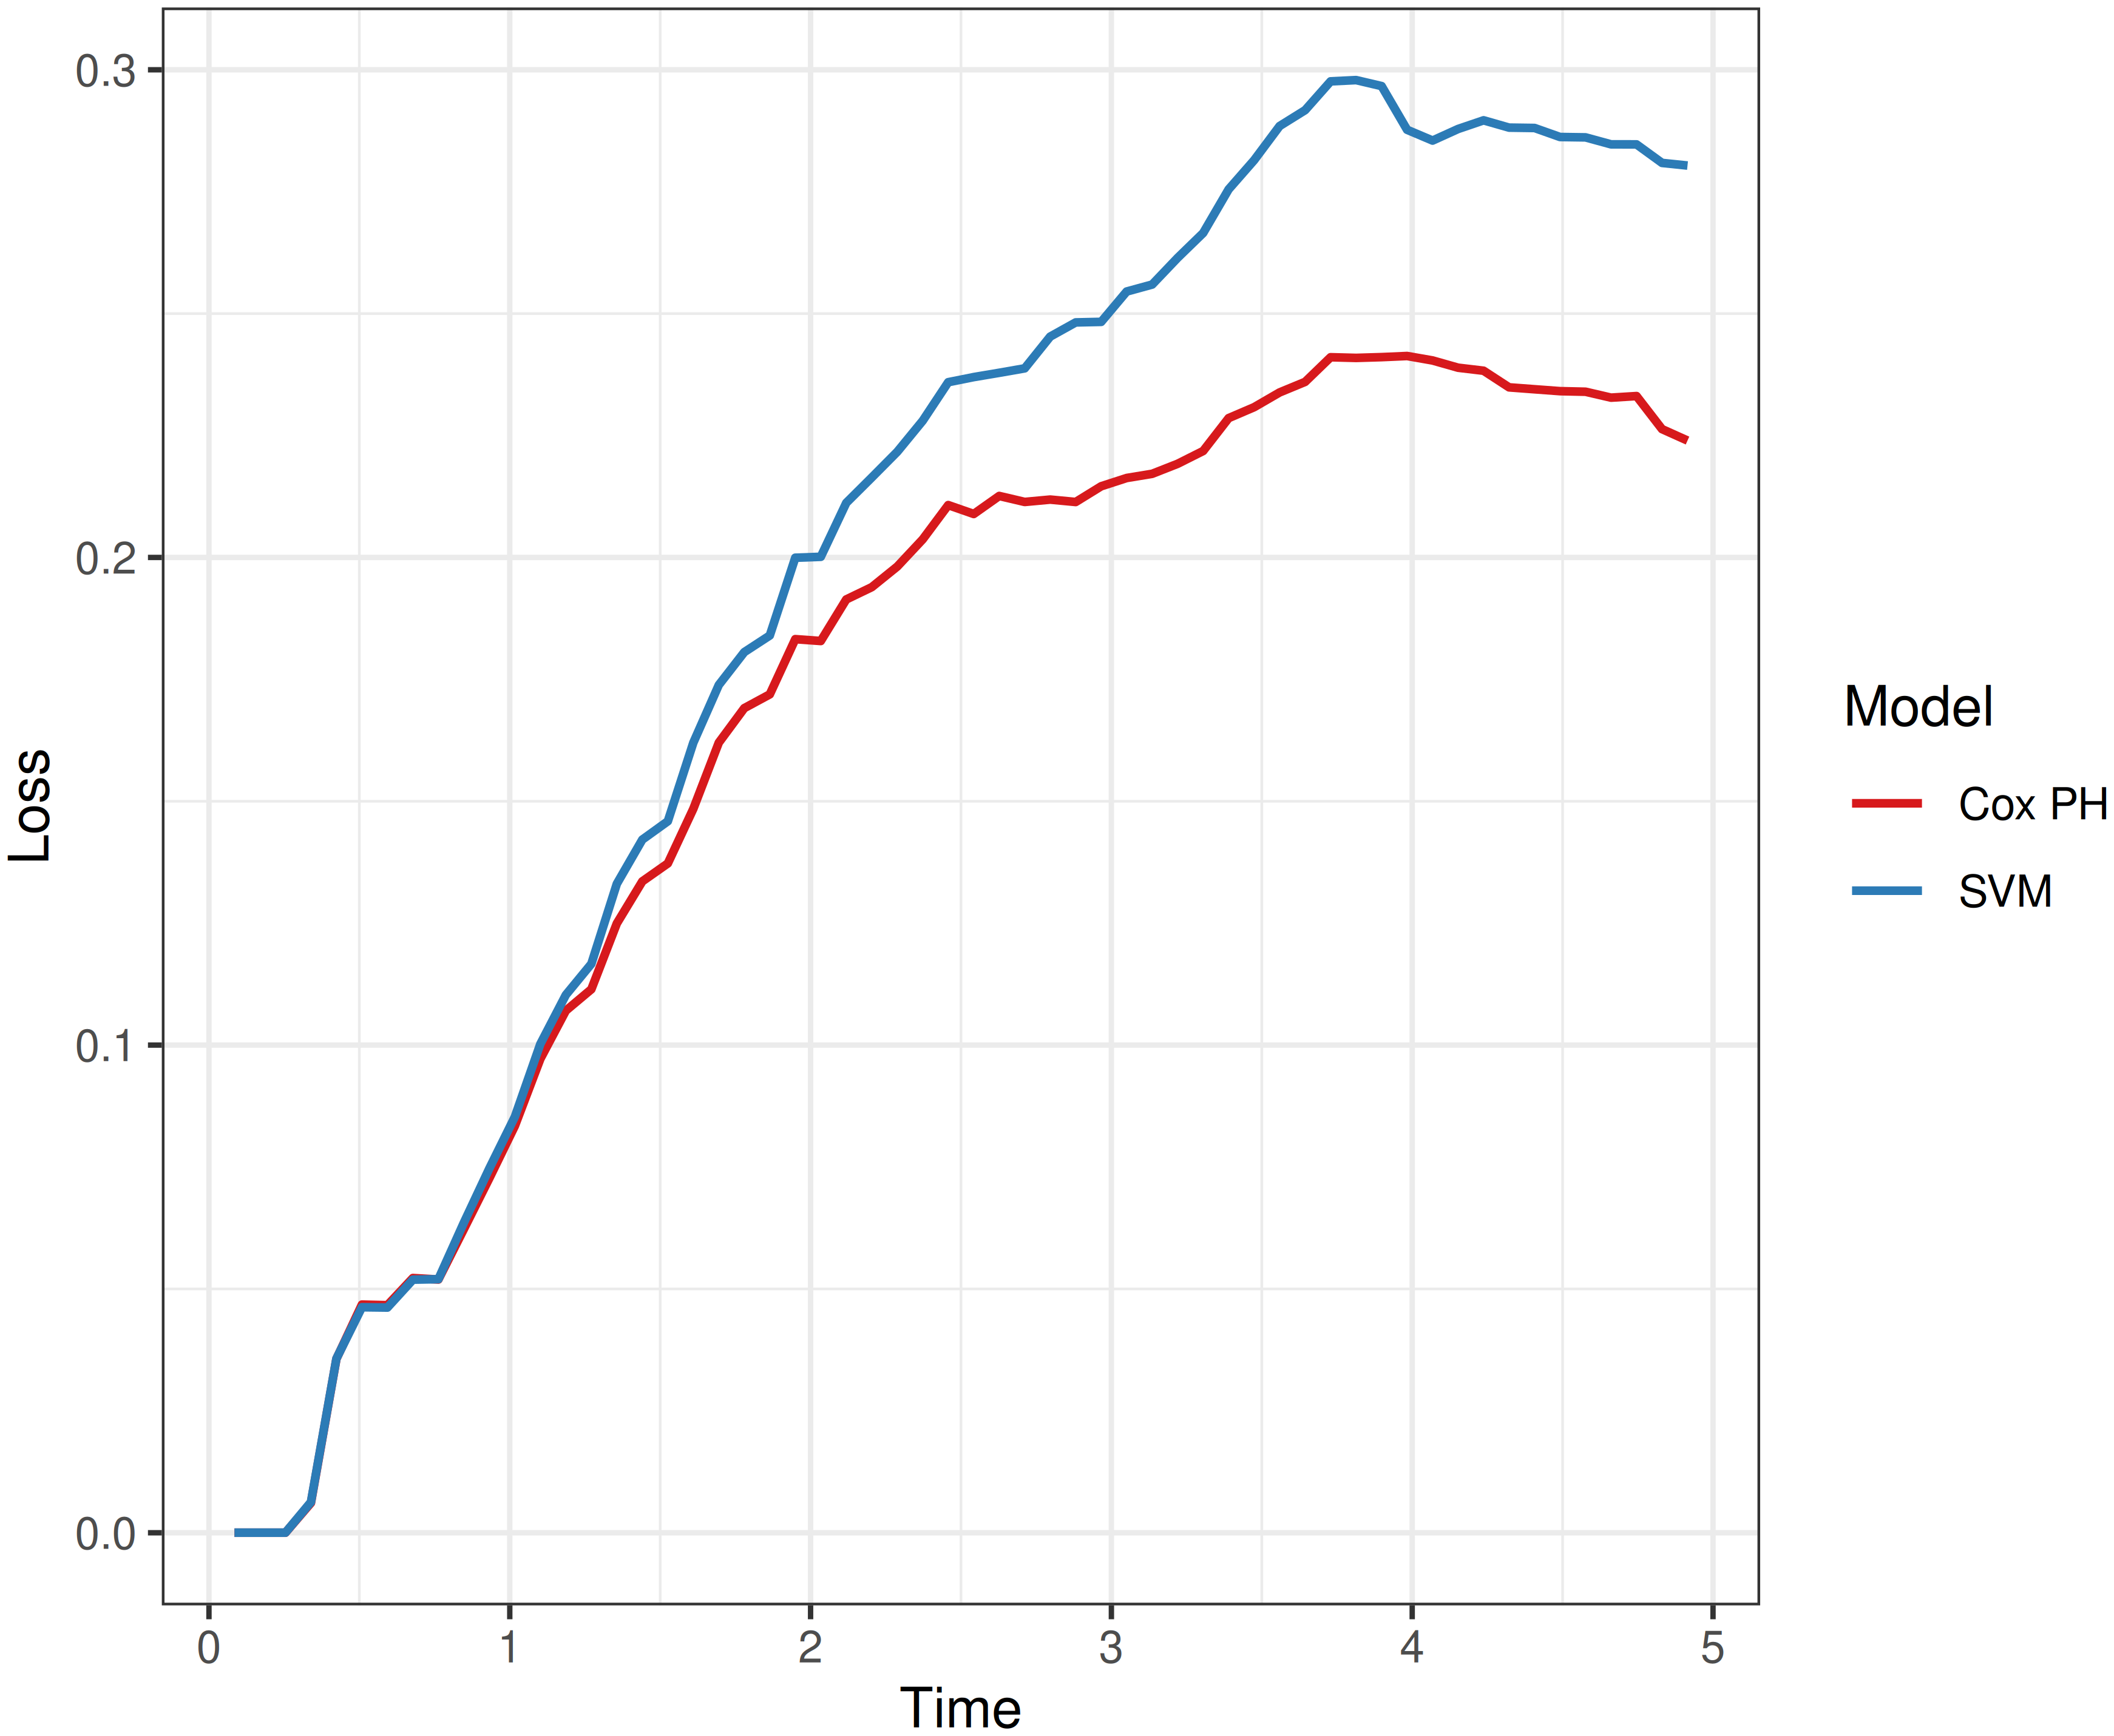
\includegraphics[width=0.7\linewidth,height=\textheight,keepaspectratio]{Figures/evaluation/fig-p2c10-pecs.png}

}

\caption{\label{fig-p2c10-pecs}Prediction error curves for a Cox PH and
an SVM model. The x-axis is time and the y-axis is the survival Brier
score computed at each time point. The Cox PH (red) appears to
increasingly perform better than the SVM (blue) over time. Trained and
tested on randomly simulated data from \texttt{mlr3proba}.}

\end{figure}%

\section{Baselines and ERV}\label{sec-eval-distr-score-base}

A common criticism of scoring rules is a lack of interpretability, for
example, an ISBS of 0.5 or 0.0005 has no meaning by itself. Two methods
can be used to help overcome this problem.

The first method is to make use of baselines\index{model baselines} for
model comparison, which are models or reference values used to
contextualize a loss and provide a common standard for judging models of
the same class. In classification, it is possible to derive analytical
baseline values, for example a Brier score is considered poor if it is
above 0.25 or a log loss if it is above 0.693
(Figure~\ref{fig-p2c10-brier-logloss}). These are the values obtained
when always predicting \(0.5\), which is the best \emph{uninformed}
baseline in a binary classification problem (equivalent to a coin flip
that uses no information from the available data). In survival analysis,
simple analytical expressions are not possible as losses are dependent
on the unknown distributions of both the survival and censoring time.
For this reason it is advisable to include baseline models for
comparison. Common baselines include the Kaplan-Meier estimator
(Section~\ref{sec-surv-km}) and Cox PH
(Section~\ref{sec-ph-semi-parametric}).
\index{Kaplan-Meier estimator}\index{Cox proportional hazards} As a rule
of thumb, a model has poor predictive ability if it performs worse than
the Kaplan-Meier, whereas outperforming the Cox PH indicates added
predictive value.

In addition to directly comparing losses from a candidate model to a
baseline, one can also compute the percentage increase in performance
between the candidate and baseline models, which produces a measure of
explained residual variation (ERV) (Edward L. Korn and Simon 1990;
Edward L. Korn and Simon 1991).\index{explained residual variation} For
any survival loss \(L\), where lower values indicate better performance
and the minimum is \(0\) (after scaling if required), the ERV is:

\[
\operatorname{ERV}_L(\hat{g}_C, \hat{g}_B) = 1 - \frac{L(\hat{g}_C)}{L(\hat{g}_B)}
\]

where \(L(\hat{g}_C)\) and \(L(\hat{g}_B)\) are the losses computed with
respect to predictions from the candidate and baseline models,
respectively.

The ERV interpretation can make scoring rules easier to interpret and
compare across experiments. For example, say a practitioner is
considering a random forest model (Chapter~\ref{sec-ranfor}) to analyze
genomics data, with performance measured using the ISBS across three
datasets. Suppose the candidate model achieves:

\[
L_1(\hat{g}_C) = 0.004; \quad L_2(\hat{g}_C) = 2.143; \quad L_3(\hat{g}_C) = 0.10.
\]

At first glance, the model appears to perform substantially worse in
dataset 2 than dataset 1. Now suppose a Kaplan-Meier estimator is used
as a baseline and achieves:

\[
L_1(\hat{g}_B) = 0.006; \quad L_2(\hat{g}_B) = 10.9; \quad L_3(\hat{g}_B) = 0.14,
\]

with corresponding ERV values:

\[
\operatorname{ERV}_{L_1}(\hat{g}_C, \hat{g}_B) = 0.33; \quad \operatorname{ERV}_{L_2}(\hat{g}_C, \hat{g}_B) = 0.80; \quad \operatorname{ERV}_{L_3}(\hat{g}_C, \hat{g}_B) = 0.29.
\]

In all three datasets the random forest outperforms the baseline, with
the largest relative improvement observed in dataset 2. This
representation can also be used across future analyses and discussions,
as relative improvements are often easier to interpret and compare than
absolute differences in loss values, especially in the presence of
censoring. For example, the \(33\%\) performance improvement in
experiment 1 is substantially more interpretable than an absolute
reduction in loss of \(0.002\), particularly because the former requires
no knowledge of the underlying loss scale or censoring distribution.

\section{Competing risks}\label{sec-rules-ext}

Similarly to discrimination measures, scoring rules are primarily used
with competing risks by evaluating cause-specific probabilities
individually (Bender et al. 2021; Geloven et al. 2022; C. Lee et al.
2018).\index{competing risks}

For example, the non-integrated, cause-specific survival Brier score for
event \(\tilde{q} \in \{1, \ldots, Q\}\) (Schoop et al. 2011) is given
by:\index{integrated survival Brier score!cause-specific}

\begin{equation}\phantomsection\label{eq-sbs-cs}{
\begin{aligned}
L_{SBS;\tilde{q}}(\tau, \{\hat{F}_{q;i}\}^Q_{q=1}, t_i, q_i \mid \hat{G}_{KM}) = {} & \frac{(1 - \hat{F}_{\tilde{q};i}(\tau))^2 \, \mathbb{I}(t_i \leq \tau, q_i = \tilde{q})}{\hat{G}_{KM}(t_i)} \\
& + \frac{\hat{F}_{\tilde{q};i}^2(\tau) \, \mathbb{I}(t_i \leq \tau, q_i \notin \{0, \tilde{q}\})}{\hat{G}_{KM}(t_i)} \\
& + \frac{\hat{F}_{\tilde{q};i}^2(\tau) \, \mathbb{I}(t_i > \tau)}{\hat{G}_{KM}(\tau)},
\end{aligned}
}\end{equation}

where \(\hat{F}_{\tilde{q};i}\) is the predicted cause-specific CIF for
cause \(\tilde{q}\), \(\hat{G}_{KM}\) is a marginal Kaplan-Meier
estimate of the censoring distribution, and \(q_i\) is the cause
experienced by observation \(i\) (with \(q_i = 0\) denoting a censored
observation). The three terms correspond to observations that, by time
\(\tau\), have experienced the cause of interest \(\tilde{q}\), have
experienced a competing event, or remain event-free, respectively;
observations censored before \(\tau\) contribute zero. When there are no
competing risks (\(Q = 1\)), \(1 - \hat{F}_{\tilde{q};i} = \hat{S}_i\)
and (\ref{eq-sbs-cs}) reduces to (\ref{eq-sbs}).

Bender et al. (2021), for example, evaluate competing-risks models using
the integrated form of this score, integrating (\ref{eq-sbs-cs}) for
each cause up to the 25th, 50th, and 75th percentiles of the observed
event times. Such cause-specific scores are currently implemented in
survival software such as \texttt{pec} and \texttt{riskRegression}
(Thomas Alexander Gerds and Ozenne 2019; Ulla B. Mogensen, Ishwaran, and
Gerds 2012). This method results in one loss per cause, which can be
useful to optimize a model for a single cause but may be less useful
when trying to optimize over all causes.

C. Lee et al. (2018) instead use a single, all-cause, discrete-time loss
similar to the RCLL\index{neural networks!survival analysis!DeepHit}:

\begin{equation}\phantomsection\label{eq-ll-deephit}{
L_{DeepHit}(\hat{S}_i, \{\hat{F}_{q;i}\}^Q_{q=1}, t_i, \delta_i, q_i) = -\log[\delta_i\hat{p}_{q_i;i}(t_i) + (1-\delta_i)\hat{S}_i(t_i)],
}\end{equation}

where \(\hat{p}_{q_i;i}(t_i)\) is the predicted probability mass for the
observed cause \(q_i\) at time \(t_i\), which can be derived from
\(\hat{F}_{q_i;i}\), and \(\delta_i\) is \(0\) if observation \(i\) is
right-censored or \(1\) if they experience any cause. This loss is the
log-likelihood term of the DeepHit training objective, which
additionally includes a ranking component to promote discrimination (C.
Lee et al. 2018). C. Lee et al. (2018) use it to train their model
rather than as an evaluation measure.

Recently, an all-cause logarithmic scoring rule, termed here the
\emph{all-cause log loss}, has been proposed, which also makes use of
IPC weighting (Alberge et al. 2025):\index{log loss!all-cause}

\begin{equation}\phantomsection\label{eq-acll}{
\begin{aligned}
& L_{ACLL}(\tau^*, \hat{S}_i, \{\hat{F}_{q;i}\}^Q_{q=1}, t_i, q_i \mid \hat{G}) = \\
& \quad -\int^{\tau^*}_0 \left[\sum^Q_{q=1} \frac{\mathbb{I}(t_i \leq \tau, q_i = q)\log(\hat{F}_{q;i}(\tau))}{\hat{G}(t_i)} + \frac{\mathbb{I}(t_i > \tau)\log(\hat{S}_i(\tau))}{\hat{G}(\tau)}\right] \,\mathrm{d}\tau,
\end{aligned}
}\end{equation}

where \(\hat{S}_i\) is the predicted all-cause survival function for
observation \(i\) and \(\hat{F}_{q;i}\) is the predicted CIF for
observation \(i\) and cause \(q\).\index{cumulative incidence function}
Alberge et al. (2025) introduce the loss in the context of a boosting
algorithm (Chapter~\ref{sec-boost}), where the censoring survival
function \(\hat{G}\) is estimated iteratively alongside the event model
(Box 3).

Note that (\ref{eq-acll}) introduces a minus sign to re-express the loss
as a quantity to be minimized, to be more consistent with other losses
in this chapter. Similarly, the integration over \([0, \tau^*]\) in
(\ref{eq-acll}) is a generalization to be consistent with the ISBS-type
definition, but is not part of the original definition in Alberge et al.
(2025).

Comparing this loss to the decomposition in
Section~\ref{sec-rules-squared}, for each cause \(q\), observations
either: experience the cause of interest, in which case their
cause-specific CIF is evaluated; neither experience an event nor are
censored by \(\tau\) and so the all-cause survival is evaluated; or
experience a different cause and contribute zero to the term for cause
\(q\).

One advantage of all-cause losses such as
(\ref{eq-ll-deephit})-(\ref{eq-acll}) is that they provide a single
scalar quantity, which is convenient for (automated) model comparison,
especially when there are many competing causes. However, this
convenience comes at a cost as optimizing a single all-cause loss can
obscure heterogeneity in performance across causes. This is especially
problematic when accurate modeling of some causes is more important than
others. Moreover, a model may achieve good overall performance while
substantially underperforming for a clinically important cause. As a
result, when performance for individual causes is a priority,
cause-specific scoring rules such as (\ref{eq-sbs-cs}) may be
preferable. In such settings, automated procedures, such as those used
for hyperparameter optimization (Chapter~\ref{sec-ml}), would require
multi-objective optimization methods (Morales-Hernández, Van
Nieuwenhuyse, and Rojas Gonzalez
2023).\index{hyperparameter optimization}

\section{Conclusion}\label{conclusion-6}

\begin{tcolorbox}[enhanced jigsaw, toprule=.15mm, bottomtitle=1mm, opacityback=0, breakable, leftrule=.75mm, title={Key takeaways}, toptitle=1mm, bottomrule=.15mm, colback=white, colframe=quarto-callout-warning-color-frame, titlerule=0mm, opacitybacktitle=0.6, coltitle=black, rightrule=.15mm, left=2mm, colbacktitle=quarto-callout-warning-color!10!white, arc=.35mm]

\begin{itemize}
\tightlist
\item
  Scoring rules are a useful tool for measuring a model's overall
  predictive ability, taking into account calibration and
  discrimination.
\item
  Proper scoring rules provide principled model comparison, which is
  important when choosing models in a benchmark experiment.
\item
  Scoring rules can be difficult to interpret but baselines and ERV
  representations can be a helpful way to overcome this.
\item
  For non- and semi-parametric survival models that return distribution
  predictions, estimates of \(f(t)\) are not readily available and
  instead require numerical approximations
  (Section~\ref{sec-distributions-continuous}). Consequently, naive
  application of logarithmic scoring rules, for example by treating a
  probability mass function as a density function, can heavily bias the
  results.
\end{itemize}

\end{tcolorbox}

\begin{tcolorbox}[enhanced jigsaw, toprule=.15mm, bottomtitle=1mm, opacityback=0, breakable, leftrule=.75mm, title={Further reading}, toptitle=1mm, bottomrule=.15mm, colback=white, colframe=quarto-callout-tip-color-frame, titlerule=0mm, opacitybacktitle=0.6, coltitle=black, rightrule=.15mm, left=2mm, colbacktitle=quarto-callout-tip-color!10!white, arc=.35mm]

\begin{itemize}
\tightlist
\item
  Alexander Philip Dawid and Musio (2014) and Gneiting and Raftery
  (2007) provide a comprehensive summary of scoring rules in regression
  and classification settings.
\item
  Rindt et al. (2022), Sonabend et al. (2025) and Yanagisawa (2023)
  review survival scoring rules, including loss forms not discussed in
  this chapter such as pinball losses.
\item
  Choodari-Oskooei, Royston, and Parmar (2012a), Choodari-Oskooei,
  Royston, and Parmar (2012b), and M. S. Rahman et al. (2017) compare
  measures for external validation including some scoring rules.
\end{itemize}

\end{tcolorbox}

\chapter{Distance Measures}\label{sec-eval-det}

As discussed in Chapter~\ref{sec-survtsk}, evaluating the distance
between point predictions of survival time and ground truth event times
is fundamentally problematic when censoring is
present.\index{survival time} In particular, there is no principled way
to define a metric that accurately reflects the average discrepancy
between predicted survival times and all event times.

The most commonly discussed distance measure in the literature is the
mean absolute error (MAE):\index{mean absolute error}

\begin{equation}\phantomsection\label{eq-mae}{
\operatorname{MAE}(\mathbf{t}, \mathbf{\hat{t}}) = \frac{1}{n} \sum^{n}_{i = 1} \vert t_i - \hat{t}_i \vert,
}\end{equation}

where \(\boldsymbol{\mathbf{t}} = ({t}_1 \ {t}_2 \cdots {t}_{n})^\top\)
and
\(\boldsymbol{\mathbf{\hat{t}}} = ({\hat{t}}_1 \ {\hat{t}}_2 \cdots {\hat{t}}_{n})^\top\)
are observed follow-up times and predicted survival times, respectively.
In the literature, (\ref{eq-mae}) is occasionally adapted for survival
analysis by restricting evaluation to uncensored observations only (P.
Wang, Li, and Reddy 2019). However, restricting evaluation in this way
introduces substantial bias. S.-A. Qi et al. (2023) show that naively
applying (\ref{eq-mae}) to uncensored data can induce model performance
rankings inconsistent with those obtained from the oracle MAE. This
remains true even when incorporating inverse probability of censoring
weights\index{inverse probability of censoring weights}.

A pseudo-value-based approach\index{pseudo-values} (see
Chapter~\ref{sec-pseudo-value-reduction} for details about
pseudo-values) has been shown, under controlled simulation settings, to
induce the same model rankings as the oracle MAE (S.-A. Qi et al. 2023).
However, this approach is not intended to, nor does it, recover a
meaningful measure of absolute distance between predicted survival times
and the ground truth event times --- pseudo-values are estimates and do
not represent the true outcome.

Given these limitations, distance-based evaluations should generally be
avoided. Instead, discrimination-based measures
(Chapter~\ref{sec-eval-crank}) may be used to evaluate survival time
predictions, while being clear that this evaluates relative risks only
and does not attempt to quantify the distance between predictions and
truth.

\section{Conclusion}\label{conclusion-7}

\begin{tcolorbox}[enhanced jigsaw, toprule=.15mm, bottomtitle=1mm, opacityback=0, breakable, leftrule=.75mm, title={Key takeaways}, toptitle=1mm, bottomrule=.15mm, colback=white, colframe=quarto-callout-warning-color-frame, titlerule=0mm, opacitybacktitle=0.6, coltitle=black, rightrule=.15mm, left=2mm, colbacktitle=quarto-callout-warning-color!10!white, arc=.35mm]

\begin{itemize}
\tightlist
\item
  Point predictions of survival time cannot be evaluated using standard
  distance-based error measures in a principled way when censoring is
  present.
\item
  Existing approaches may support relative comparison of models but do
  not resolve the fundamental ambiguity created by unobserved event
  times.
\item
  As a result, discrimination-based evaluation should be preferred, with
  careful interpretation of what is, and is not, being evaluated.
\end{itemize}

\end{tcolorbox}

\chapter{Choosing Measures}\label{sec-choosing-measures}

There are many survival measures\index{performance measure} to choose
from, and selecting the right one for a given task may seem daunting.
Below are a few heuristics to support decision-making. First and
foremost, evaluation should always be according to the goals of
analysis, which means using discrimination
measures\index{discrimination} to evaluate relative risk
predictions\index{relative risk}, calibration\index{calibration}
measures to evaluate average agreement between predicted and empirical
outcome distributions, and scoring rules\index{scoring rules} to
evaluate overall performance and distribution predictions.

For discrimination measures, consider Harrell's C and Uno's
C.\index{concordance index!Harrell's C}\index{concordance index!Uno's C}
While other discrimination measures can assess time-dependent ranking
performance, time-dependent predictive performance can also be examined
through scoring rules. If only one measure is to be reported, then Uno's
C may be preferred. Although Uno's C can have higher variance than
Harrell's C (M. S. Rahman et al. 2017; Schmid and Potapov 2012), it is
less likely to overestimate concordance as censoring increases (M. S.
Rahman et al. 2017). Moreover, the variance can be transparently
captured and reported through techniques such as bootstrapping. In
practice, the choice of measure matters less than ensuring your
reporting is transparent and honest (Sonabend, Bender, and Vollmer 2022;
Therneau and Atkinson 2024).\index{C-hacking}

To assess the calibration of a single model, graphical comparisons to
the Kaplan-Meier estimator\index{Kaplan-Meier estimator} provide a
useful and interpretable way to assess model fit
(Section~\ref{sec-calib-km}). \index{calibration!plots} When choosing
between models, D-calibration\index{calibration!D-calibration} provides
a quantitative statistic with a meaningful minimum and therefore can be
used as a tool for model comparison.

When choosing scoring rules, the survival Brier score (\ref{eq-sbs})
provides a useful score for developing prediction error curves
(Section~\ref{sec-pecs}). For a quantity that summarizes overall
predictive ability, the integrated SBS (\ref{eq-igs}) is most commonly
used in the literature though its properness is susceptible to different
censoring patterns. The RCLL\index{right-censored log loss}
(Section~\ref{sec-rules-log}) is intuitive and is proven strictly proper
when censoring is conditionally event-independent (Rindt et al. 2022;
Yanagisawa 2023), but may require numerical approximation of the density
function (Section~\ref{sec-distributions-continuous}). Most importantly,
the choice of evaluation measures should be decided up front and not
selected based on preliminary results. When reporting scoring rules,
consider the ERV representation which provides a meaningful
interpretation as relative performance compared with a standard
baseline.\index{explained residual variation}

Given the limited research currently available, evaluation of survival
time predictions should be treated with caution and new developments in
the literature should be monitored.

For automated model optimization\index{hyperparameter optimization},
tuning with a scoring rule should capture discrimination and calibration
simultaneously (Kopper et al. 2026; Rindt et al. 2022; Yanagisawa 2023).
However, if you are developing a model to maximize separation and
calibration truly matters less, then prefer Harrell's C over Uno's C, as
any bias in the measure should affect models similarly, making lower
variance potentially preferable. Finally, avoid using a measure of
calibration alone for tuning, as this can favor models that approximate
marginal non-parametric estimates rather than individualized
predictions.

\part{Models}

\chapter{Core Estimators, Models, and Methods}\label{sec-classical}

In a predictive setting, it can be easy to dismiss survival models that
have been around for decades and instead favor testing of more modern
`machine learning' tools. This would be a mistake. First, most machine
learning survival algorithms build on these models as a central
component, for example by using non-parametric estimators
(Section~\ref{sec-classical-nonpar}) and/or assuming a proportional
hazards form (Section~\ref{sec-classical-cox}). For this reason, this
book refers to them as core models. Second, on low-dimensional data
(small number of variables), these core models often outperform machine
learning models (Beaulac et al. 2020; Burk et al. 2026). Finally, even
on high-dimensional data\index{high-dimensional data}, several papers
have demonstrated that augmenting core models
(Section~\ref{sec-classical-improving}) can yield models that outperform
machine learning alternatives (Spooner et al. 2020; Y. Zhang et al.
2022). Therefore, a robust understanding of these models is imperative
to fairly construct and evaluate machine learning survival models.

This chapter begins by demonstrating non-parametric estimators as
predictive tools, including a recap of some estimators in
Chapter~\ref{sec-surv}. Semi- and fully-parametric models are then
introduced, most notably the Cox proportional hazards model
(Section~\ref{sec-ph-semi-parametric}) and the accelerated failure time
model (Section~\ref{sec-surv-models-param}). Finally, the chapter
presents core methods (Section~\ref{sec-classical-improving}) that are
used throughout survival analysis and can improve the predictive
performance of core models, including non-linear modeling, feature
selection, regularization, and ensemble learning.

\section{Non-parametric estimators}\label{sec-classical-nonpar}

Non-parametric estimators\index{non-parametric estimator} have already
been introduced in Section~\ref{sec-surv-estimation-non-param},
therefore this section is brief and focuses only on how these estimators
can be used as predictive models.

\subsection{Unconditional estimators}\label{unconditional-estimators}

Recall from Section~\ref{sec-surv-estimation-non-param}, the
Kaplan-Meier\index{Kaplan-Meier estimator} and
Nelson-Aalen\index{Nelson-Aalen estimator} estimators respectively
estimate the survival function and cumulative hazard function as:

\begin{equation}\phantomsection\label{eq-km-ml-two}{
S_{KM}(\tau) = \prod_{k:t_{(k)} \leq \tau}\left(1-\frac{d_{t_{(k)}}}{n_{t_{(k)}}}\right),
}\end{equation}

and

\[
H_{NA}(\tau) = \sum_{k:t_{(k)}\leq \tau} \frac{d_{t_{(k)}}}{n_{t_{(k)}}},
\]

where \(d_{t_{(k)}}\) and \(n_{t_{(k)}}\) are the number of events and
observations at risk at the \(k\)th ordered event time, \(t_{(k)}\)
respectively.

Figure~\ref{fig-p3c13-km-test} illustrates the Kaplan-Meier estimator
fit on the \texttt{rats} (Mantel, Bohidar, and Ciminera 1977) dataset.
The left image shows the estimator as a step function, with steps
occurring at event times (some examples in green dashed lines). At
censoring times, the estimator stays constant (examples in blue dotted
lines). The right image displays the estimator as a predictive tool. To
predict the survival probability of a new rat, one can find the
estimated survival probability at a given time from the trained
estimator, without needing any more details about the rat in question
(as covariates are ignored). This provides a quick tool that tends to be
marginally well-calibrated (Chapter~\ref{sec-eval-distr-calib}). This
estimator is the analogue to the sample mode and sample mean baseline
estimators\index{baseline model} in classification and regression
respectively. The same idea of using a non-parametric featureless
estimator as a predictive baseline follows for other censoring and
truncation types (Section~\ref{sec-surv-estimation-non-param}) and event
history analysis more generally (Section~\ref{sec-aalen-johansen}).

\begin{figure}

\centering{

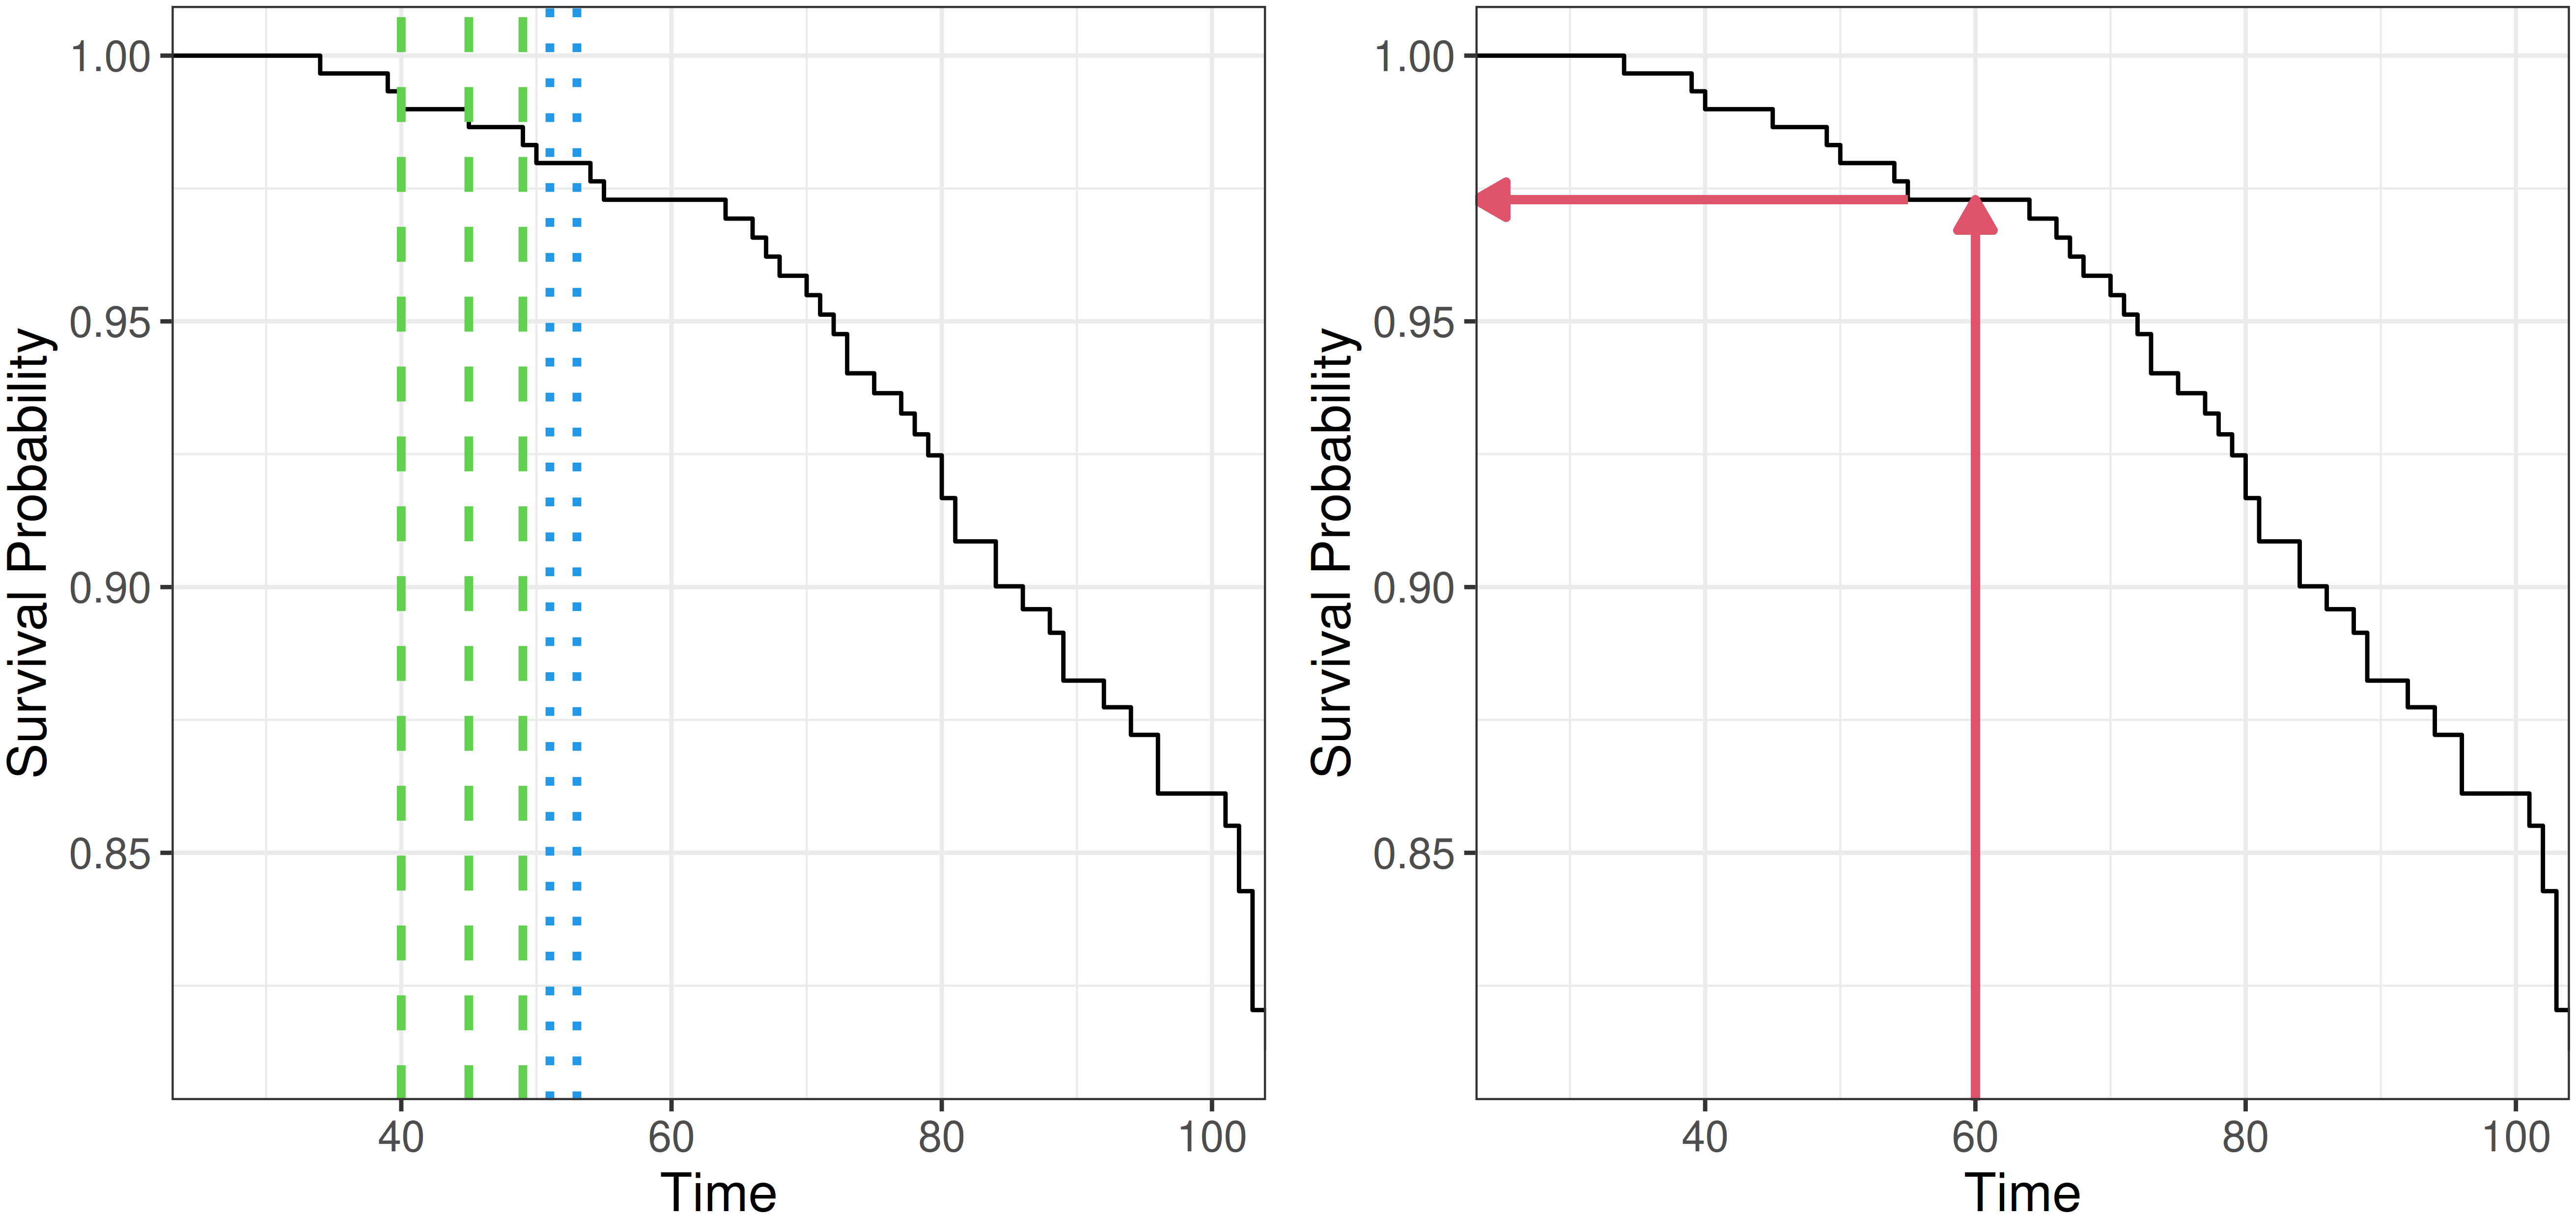
\includegraphics[width=1\linewidth,height=\textheight,keepaspectratio]{Figures/classical/fig-p3c13-km-test.png}

}

\caption{\label{fig-p3c13-km-test}Using the Kaplan-Meier estimator as a
predictive tool. The left image shows the estimator fit to data, the
green dashed lines are steps in the function at event times and the blue
dotted lines are censoring times in the training data and no steps
occur. The right image demonstrates using the estimator as a predictive
tool by reading off the survival probability at given times.}

\end{figure}%

\subsection{Conditional estimators}\label{conditional-estimators}

As well as unconditional estimators, which do not account for
covariates, an alternative is the conditional Akritas estimator (Michael
G. Akritas 1994), usually defined by (Blanche, Dartigues, and
Jacqmin-Gadda 2013):\index{Akritas estimator}

\begin{equation}\phantomsection\label{eq-akritas}{
S(\tau \mid \mathbf{x}^*, \lambda) = \prod_{k:t_{(k)}\leq \tau} \left(1 - \frac{\sum^n_{i=1} K(\mathbf{x}^*,\mathbf{x}_i \mid \lambda)\mathbb{I}(t_i = t_{(k)}, \delta_i = 1)}{\sum^n_{i=1} K(\mathbf{x}^*,\mathbf{x}_i \mid \lambda)\mathbb{I}(t_i \geq t_{(k)})}\right),
}\end{equation}

where \(K\) is a kernel function, usually
\(K(\mathbf{x},\mathbf{y}\mid \lambda) = \mathbb{I}(\lvert \hat{F}_X(\mathbf{x}) - \hat{F}_X(\mathbf{y})\rvert \leq \lambda), \lambda \in (0, 1]\)
is a hyperparameter, and \(\hat{F}_X\) is the empirical distribution
function of the data. The estimator can be interpreted as a conditional
Kaplan-Meier estimator computed on a neighborhood of subjects closest to
\(\mathbf{x}^*\). When \(\lambda = 1\), then
\(K(\cdot \mid \lambda) = 1\) and (\ref{eq-akritas}) is identical to
(\ref{eq-km-ml-two}).

The formulation in (\ref{eq-akritas}) can be turned into a baseline
predictive model by treating estimation of \(\hat{F}_X\) on training
data as the learning algorithm, and then using (\ref{eq-akritas}) as the
prediction algorithm (Section~\ref{sec-ml-models}).
\index{baseline model}

\section{Proportional hazards}\label{sec-classical-cox}

This section begins with an introduction to the proportional hazards
concept\index{proportional hazards}, introduces estimation with the Cox
proportional hazards\index{Cox proportional hazards} model
(Section~\ref{sec-ph-semi-parametric}), and then moves to fully
parametric proportional hazards models
(Section~\ref{sec-ph-parametric}), with the Weibull model as a
motivating example.\index{proportional hazards!fully parametric}

Let \(\eta_i = \mathbf{x}_i^\top\boldsymbol{\beta}\) be the linear
predictor for some observation \(i\) with covariates
\(\mathbf{x}_i \in \mathbb{R}^p\) and model coefficients
\(\boldsymbol{\beta}\in \mathbb{R}^p\), then proportional hazards (PH)
models assume that the hazard function for observation \(i\) follows the
form:

\begin{equation}\phantomsection\label{eq-ph}{
h_{PH}(\tau \mid \mathbf{x}_i)= h_0(\tau)\exp(\eta_i),
}\end{equation}

or equivalently:

\begin{equation}\phantomsection\label{eq-ph-cum}{
H_{PH}(\tau \mid \mathbf{x}_i)= H_0(\tau)\exp(\eta_i),
}\end{equation}

and

\begin{equation}\phantomsection\label{eq-ph-surv}{
S_{PH}(\tau \mid \mathbf{x}_i)= S_0(\tau)^{\exp(\eta_i)}.
}\end{equation}

\(h_0,H_0,S_0\) are referred to as the baseline hazard, cumulative
hazard, and survival function
respectively.\index{baseline hazard}\index{baseline survival function}
Instead of modeling a separate intercept, the \emph{baseline hazard}
represents the hazard when the linear predictor is zero, hence the term
\emph{baseline}. Note that the baseline hazard may not have a meaningful
interpretation unless continuous covariates are centered and categorical
covariates are reference coded (analogous to the intercept \(\beta_0\)
in linear regression).

It can be seen from (\ref{eq-ph}) that time is only incorporated via the
baseline hazard (see Houwelingen and Putter 2011 for extensions to
time-varying covariates).\index{time-varying covariates} Therefore, PH
models first estimate the baseline risk of an event at a fixed time, and
then modulate this risk according to the specification of covariates.
This represents the eponymous `proportional hazards' assumption as the
individual's hazard at time \(\tau\) is directly proportional to a
multiplicative function of their own covariates:
\(h(\tau \mid \mathbf{x}_i) \propto \exp(\eta_i)\).\index{proportional hazards!assumption}
In other words, a unit change in a covariate acts multiplicatively on
the estimated hazard. For a single covariate \(x\), the \emph{hazard
ratio} is:\index{proportional hazards!hazard ratio}

\begin{equation}\phantomsection\label{eq-ph-hazard-ratio}{
\frac{h_{PH}(\tau \mid x_i)}{h_{PH}(\tau \mid x_j)} = \frac{h_0(\tau)\exp(x_i\beta)}{h_0(\tau)\exp(x_j\beta)} = \exp(\beta(x_i -x_j)),
}\end{equation}

or equivalently:

\[
h_{PH}(\tau \mid x_i) = \exp(\beta(x_i - x_j))h_{PH}(\tau \mid x_j).
\]

So in the case where the covariate differs between subjects by \(1\),
the hazard ratio is \(\exp(\beta)\). This yields an interpretable model
in which hazard ratios depend solely on the value of their linear
predictors and remain constant over time. This does \emph{not} imply
that the effect of covariates on the survival function is constant over
time, as the survival ratio depends on \(S_0\):

\[
\frac{S_{PH}(\tau \mid x_i)}{S_{PH}(\tau \mid x_j)} = \frac{S_0(\tau)^{\exp(x_i\beta)}}{S_0(\tau)^{\exp(x_j\beta)}} = S_0(\tau)^{\exp(x_i\beta)-\exp(x_j\beta)}.
\]

The next sections discuss how to fit the \(\boldsymbol{\beta}\)
parameters semi-parametrically (Section~\ref{sec-ph-semi-parametric})
and fully parametrically (Section~\ref{sec-ph-parametric}).

\subsection{Semi-parametric PH}\label{sec-ph-semi-parametric}

The Cox proportional hazards (Cox PH) (Cox 1972), or Cox model, is
likely the most widely known semi-parametric model and the most studied
survival model (Reid 1994; P. Wang, Li, and Reddy
2019).\index{Cox proportional hazards}\index{proportional hazards!semi-parametric}
Often, it is considered synonymous with proportional hazards and the
functional form of the hazard given in (\ref{eq-ph}). However, the main
contribution of Cox's work was to develop a method to estimate
\(\boldsymbol{\beta}\) without making any assumptions about the baseline
hazard. \index{baseline hazard} Estimation of the parameters is
discussed in detail as the objective function of the Cox model is also
used by many machine learning methods like boosting
(Chapter~\ref{sec-boost}) and neural networks (Chapter~\ref{sec-nnet}).

Recall from Section~\ref{sec-surv-estimation}, to estimate the
distribution of event times one either needs to make distributional
assumptions and accordingly define the likelihood of observing the data
(given model parameters), or to use non-parametric estimators, which
usually do not incorporate covariate information. Let \(i_{(k)}\) denote
the subject who experienced the event at ordered event time \(t_{(k)}\).
Cox noted the contribution of an individual could be defined as the
probability of a subject, \(i_{(k)}\), experiencing the event at
\(t_{(k)}\), given that someone in the risk set experienced the event at
that time. The likelihood contribution of this \(k\)th event is given
by:

\[
\mathcal{L}^{Cox}_{i_{(k)}}
=\frac{h_0\left(t_{(k)}\right)\exp\left(\eta_{i_{(k)}}\right)}
{\sum_{j\in \mathcal{R}_{t_{(k)}}} h_0\left(t_{(k)}\right)\exp\left(\eta_j\right)}
=\frac{\exp\left(\eta_{i_{(k)}}\right)}
{\sum_{j\in \mathcal{R}_{t_{(k)}}}\exp\left(\eta_j\right)},
\]

which depends on \(\boldsymbol{\beta}\) via
\(\eta_i=\mathbf{x}_i^\top\boldsymbol{\beta}\). Note how the baseline
hazard \(h_0\) cancels out in the likelihood contribution and removes
the dependency on the exact event time. For the estimation of
\(\boldsymbol{\beta}\), the baseline hazard can be considered a
`nuisance parameter'\index{baseline hazard} and the likelihood for the
entire data set can be defined as:
\index{Cox proportional hazards!partial likelihood}

\begin{equation}\phantomsection\label{eq-partial}{
\mathcal{L}_{PL}(\boldsymbol{\beta}) = \prod_{k=1}^m \mathcal{L}^{Cox}_{i_{(k)}} = \prod_{k=1}^m \left(\frac{\exp(\eta_{i_{(k)}})}{\sum_{j \in \mathcal{R}_{t_{(k)}}} \exp(\eta_j)}\right),
}\end{equation}

which is referred to as a \emph{partial likelihood} (Cox 1975) as it
omits the baseline hazard and so captures only part of the full
likelihood, rather than fully specifying the distribution of event
times. Ignoring the baseline hazard means that exact event time
information is absent from (\ref{eq-partial}). However, observation
rankings are still preserved as event time information contributes to
(\ref{eq-partial}) through the index of the product and sum. Censored
observations contribute to the likelihood through \(\exp(\eta_j)\) in
the denominator of the calculation.

The partial likelihood (\ref{eq-partial}) assumes there are no ties in
the event time, that is, no two subjects have an event at the same time.
In practice, ties can be common and several methods have been proposed
to handle them, including an exact (but computationally expensive)
method (J. D. Kalbfleisch and Prentice 1973), the Breslow approximation
(Breslow 1974), and the Efron approximation (Efron 1977). Further
details are not discussed here, but all three methods are readily
accessible in openly available software.\index{ties}

The log-partial likelihood, usually preferred for optimization, is given
by:\index{Cox proportional hazards!log-partial likelihood}

\begin{equation}\phantomsection\label{eq-lpartial}{
\ell_{PL}(\boldsymbol{\beta}) = \sum_{k=1}^m \left(\eta_{i_{(k)}} - \log \left(\sum_{j \in \mathcal{R}_{t_{(k)}}} \exp(\eta_j)\right)\right),
}\end{equation}

such that

\begin{equation}\phantomsection\label{eq-estimate-beta}{
\hat{\boldsymbol{\beta}} = \mathop{\mathrm{arg\,max}}_{\boldsymbol{\beta}}\ \ell_{PL}(\boldsymbol{\beta}).
}\end{equation}

Traditionally, \(\hat{\boldsymbol{\beta}}\) is obtained using numerical
optimization methods, such as Newton-Raphson or Fisher-Scoring, which
require the first and second derivatives of (\ref{eq-lpartial}).

The partial likelihood allows estimation of covariate effects (and
interpretation in terms of hazard ratios) without making any assumptions
about the underlying distribution of event times. Obtaining
\(\hat{\boldsymbol{\beta}}\) also provides enough information to make
predictions in the form of relative risks
(Section~\ref{sec-survtsk-risk}). However, making survival distribution
predictions (Section~\ref{sec-survtsk-dist}) requires an estimate of the
baseline hazard, \(h_0\). The Breslow
estimator\index{Cox proportional hazards!Breslow estimator} (Breslow
1972; Lin 2007) provides a way to obtain an estimate of the cumulative
baseline hazard, \(H_0\), using the parameters from the Cox model:

\begin{equation}\phantomsection\label{eq-breslow}{
H_{Bres}(\tau) = H_0(\tau) = \sum_{k:t_{(k)}\leq \tau} \frac{d_{t_{(k)}}}{\sum_{j \in \mathcal{R}_{t_{(k)}}} \exp(\eta_j)}.
}\end{equation}

The Breslow estimator is identical to the Nelson-Aalen
estimator\index{Nelson-Aalen estimator} (\ref{eq-nelson-aalen}) when the
linear predictor is zero for every observation:

\[
H_{Bres}(\tau) = \sum_{k:t_{(k)}\leq \tau} \frac{d_{t_{(k)}}}{\sum_{j \in \mathcal{R}_{t_{(k)}}} 1} = \sum_{t_{(k)}\leq \tau} \frac{d_{t_{(k)}}}{n_{t_{(k)}}} = H_{NA}(\tau).
\]

With these formulae, the Cox PH model can be used as a predictive model.
The learning and prediction algorithms each proceed in two steps:

\begin{enumerate}
\def\labelenumi{\arabic{enumi}.}
\tightlist
\item
  Learning: Fit \(\hat{\boldsymbol{\beta}}\) on training data via
  (\ref{eq-estimate-beta}) and then estimate the cumulative baseline
  hazard, \(\hat{H}_0\) with (\ref{eq-breslow}).
\item
  Predicting: Use \(\hat{\boldsymbol{\beta}}\) to obtain
  \(\hat{\eta}_i\) for new observations, optionally returning
  \(\exp(\hat{\eta}_i)\) as a relative risk prediction. Then combine
  \(\hat{\eta}_i\) with \(\hat{H}_0\) via (\ref{eq-ph-cum}) to return a
  predicted survival distribution.
\end{enumerate}

The Cox model is highly interpretable and has a long history of use in
clinical prediction modeling and analysis. However, the proportional
hazards assumption is often violated in practice. Over the years,
extensions to the Cox model have been developed (Therneau and Grambsch
2001) to incorporate stratified baseline hazards (where the PH
assumption only has to hold within strata), time-varying effects (where
the effects of time-constant covariates change over time), and
time-varying covariates (where covariate values themselves change over
time). While these extensions can improve model fit and support
interpretation, they may be difficult to incorporate into predictive
modeling, particularly when future covariate values are unknown. Even
without such extensions, the Cox model has been shown to perform well in
comparison to more complex models in neutral benchmark experiments (Burk
et al. 2026; Michael F. Gensheimer and Narasimhan 2019a; Luxhoj and
Shyur 1997; Van Belle et al. 2011).

\subsection{Parametric PH}\label{sec-ph-parametric}

Semi-parametric approaches (like the Cox model) are popular because they
do not make an assumption about the underlying distribution of event
times, leaving the baseline hazard unspecified. However, there are some
cases where modeling a particular distribution is
sensible.\index{proportional hazards!fully parametric} On these
occasions, a specific probability distribution of the event times is
assumed, with three common choices being the exponential, Gompertz, and
Weibull distributions (John D. Kalbfleisch and Prentice 1980; P. Wang,
Li, and Reddy
2019).\index{exponential distribution}\index{Weibull distribution}\index{Gompertz distribution}
The exponential distribution is a special case of the Weibull
distribution when the latter's shape parameter equals \(1\).

Assuming a PH model, one can plug in the hazard and survival functions
from the Weibull distribution into (\ref{eq-ph}) and (\ref{eq-ph-surv})
respectively. First recall for a
\(\operatorname{Weibull}(\gamma, \lambda)\) distribution with shape
parameter \(\gamma\) and scale parameter \(\lambda\), the relevant
functions can be given by (John D. Kalbfleisch and Prentice
1980):\index{proportional hazards!Weibull}\index{proportional hazards!exponential}

\[
h(\tau) = \lambda\gamma \tau^{\gamma-1} \quad \text{and} \quad S(\tau) = \exp(-\lambda \tau^\gamma).
\]

These functions can be substituted into the PH form as the baseline
hazard and survival functions respectively:

\begin{equation}\phantomsection\label{eq-ph-weibull-haz}{
h_{WeibullPH}(\tau \mid \mathbf{x}_i)= (\lambda\gamma \tau^{\gamma-1}) \exp(\eta_i),
}\end{equation} or equivalently
\begin{equation}\phantomsection\label{eq-ph-weibull-surv}{
S_{WeibullPH}(\tau \mid \mathbf{x}_i)= (\exp(-\lambda \tau^\gamma))^{\exp(\eta_i)}.
}\end{equation}

The full likelihood (Section~\ref{sec-surv-estimation-param}) for the
WeibullPH model follows by substituting
(\ref{eq-ph-weibull-haz})-(\ref{eq-ph-weibull-surv}) into the
right-censored likelihood (\ref{eq-right-censoring-likelihood}):

\[
\begin{aligned}
\mathcal{L}(\boldsymbol{\theta}) &= \prod_{i=1}^n h_Y(t_i \mid \mathbf{x}_i, \boldsymbol{\theta})^{\delta_i}S_Y(t_i \mid \mathbf{x}_i, \boldsymbol{\theta}) \\
&= \prod_{i=1}^n \left(\lambda\gamma t_i^{\gamma-1} \exp\left(\eta_i\right)\right)^{\delta_i}\left(\exp\left(-\lambda t_i^\gamma\right)\right)^{\exp(\eta_i)},
\end{aligned}
\]

with log-likelihood:

\[
\begin{aligned}
\ell(\boldsymbol{\theta}) &= \sum_{i=1}^n \delta_i[\log(\lambda\gamma) + (\gamma-1)\log(t_i) + \eta_i] - \lambda t_i^\gamma\exp(\eta_i) \\
&\propto \sum_{i=1}^n \delta_i[\log(\lambda\gamma) + \gamma\log(t_i) + \eta_i] - \lambda t_i^\gamma \exp(\eta_i).
\end{aligned}
\]

Parameters can then be fit using maximum likelihood
estimation\index{maximum likelihood estimator} with respect to all
unknown parameters
\(\boldsymbol{\theta}= \{\boldsymbol{\beta}, \gamma, \lambda\}\).
Expansion to other censoring types and truncation follows by using other
likelihood forms presented in Section~\ref{sec-surv-estimation}.

When considering which probability distributions to model in predictive
experiments, Weibull is a common starting choice (R. and J. 1968;
Hielscher et al. 2010; M. S. Rahman et al. 2017), its two parameters
make it a flexible fit to data but on the other hand it can be easily
reduced to exponential when \(\gamma=1\). Gompertz (Gompertz 1825) is
commonly used in medical domains, especially when describing adult
lifespans.\index{Gompertz distribution}\index{Weibull distribution} In a
machine learning context, one can select the optimal distribution for
future predictive performance by running a benchmark experiment. In
contrast to the semi-parametric Cox model, fully parametric PH models
can predict absolutely continuous survival distributions, they do not
treat the baseline hazard as a nuisance, and in general will result in
more precise and interpretable predictions if the distribution is
correctly specified (Reid 1994; Royston and Parmar 2002).

\subsection{Competing risks}\label{sec-classical-ph-cr}

There are two common methods to extend the Cox model to the competing
risks setting.\index{competing risks} The first makes use of the
cause-specific hazard to fit a cause-specific Cox model, the second fits
a `subdistribution'
hazard.\index{proportional hazards!cause-specific}\index{proportional hazards!subdistribution}

\subsubsection{Cause-specific PH models}\label{cause-specific-ph-models}

In cause-specific models, the hazard for cause \(q \in \{1,\ldots,Q\}\)
is defined as:\index{proportional hazards!cause-specific}

\[
h_{q}(\tau \mid \mathbf{x}_{q;i})= h_{q;0}(\tau)\exp(\eta_{q;i}),
\]

where \(h_{q;0}\) is a cause-specific baseline hazard and
\(\mathbf{x}_{q;i}\) is a set of cause-specific covariates (in practice,
usually the same covariates are used for all causes), and \(\eta_{q;i}\)
is the cause-specific linear predictor,

\[
\eta_{q;i} = \mathbf{x}_{q;i}^\top\boldsymbol{\beta}_q.
\]

To estimate \(\boldsymbol{\beta}_q\), let \(t_{q;(k)}, k=1,\ldots,m(q)\)
be the unique, ordered event times at which events of cause \(q\) occur
and let \(i_{q;(k)}\) be the index of the observation that experiences
the \(k\)th event of cause \(q\). Then the cause-specific partial
likelihood is given by:

\begin{equation}\phantomsection\label{eq-partial-cr}{
\mathcal{L}_{PL}(\boldsymbol{\beta}_q) = \prod_{k=1}^{m(q)} \left(\frac{\exp(\eta_{q;i_{q;(k)}})}{\sum_{j \in \mathcal{R}_{t_{q;(k)}}} \exp(\eta_{q;j})}\right),
}\end{equation}

where \(\mathcal{R}_{t_{q;(k)}}\) is the risk set of observations that
have not experienced an event of \emph{any} cause or censoring before
\(t_{q;(k)}\). The competing risks partial likelihood
(\ref{eq-partial-cr}) is identical to the single-event partial
likelihood in (\ref{eq-partial}), with the only difference being that
the product and sum are over the unique, ordered event times for cause
\(q\). \index{proportional hazards!cause-specific partial likelihood}

Using the same logic as in the single-event case, the Breslow estimator
follows from (\ref{eq-breslow}):
\index{Cox proportional hazards!Breslow estimator}

\[
H_{Bres;q}(\tau) = \sum_{k:t_{q;(k)}\leq \tau} \frac{d_{t_{q;(k)}}}{\sum_{j \in \mathcal{R}_{t_{q;(k)}}} \exp(\eta_{q;j})},
\]

and the feature-dependent, cause-specific cumulative hazard
(\ref{eq-ph-cum}) as,\index{cause-specific cumulative hazard function}

\begin{equation}\phantomsection\label{eq-cause-specific-cumu-hazard-cox}{
H_{q}(\tau \mid \mathbf{x}) = H_{Bres;q}(\tau)\exp(\mathbf{x}^\top\boldsymbol{\beta}_q).
}\end{equation}

A final prediction of the cumulative incidence
function\index{cumulative incidence function} follows by (\ref{eq-cif})
where the cause-specific hazard
function\index{cause-specific hazard function} is the derivative (or a
discrete approximation) of (\ref{eq-cause-specific-cumu-hazard-cox}) and
the all-cause survival probability\index{all-cause survival function}
follows by (\ref{eq-all-cause-surv-prob}):
\begin{equation}\phantomsection\label{eq-cif-cox}{
\begin{aligned}
&F_{Bres;q}(\tau \mid \mathbf{x}) = \\
&\sum_{k:t_{q;(k)}\leq \tau} \exp\left(-\sum_{r=1}^Q H_{r}(t_{q;(k)}- \mid \mathbf{x})\right) \frac{d_{t_{q;(k)}}}{\sum_{j \in \mathcal{R}_{t_{q;(k)}}} \exp(\eta_{q;j})}\exp(\mathbf{x}^\top\boldsymbol{\beta}_q).
\end{aligned}
}\end{equation}

\subsubsection{Subdistribution PH
models}\label{subdistribution-ph-models}

The methods discussed thus far estimate cause-specific hazards
(\ref{eq-cause-specific-hazard}), which represent the instantaneous risk
of an individual experiencing the cause of interest, given that they
have not yet experienced \emph{any} event.
\index{proportional hazards!subdistribution} An alternative approach is
to model subdistribution hazards, which model the risk of an individual
experiencing the cause of interest, given they have not yet experienced
the event of interest, but may have experienced a competing event. One
benefit of the subdistribution model is the ability to directly relate
the covariates to the cumulative incidence function (CIF) under a PH
model, rather than using the indirect calculation in (\ref{eq-cif-cox}).

Mathematically, the difference between cause-specific and
subdistribution hazards comes from the definition of the risk set. The
subdistribution risk set is defined as: \index{risk set!subdistribution}
\begin{equation}\phantomsection\label{eq-riskset-sd}{
\mathcal{R}^{SD}_{q;\tau} := \{i: t_i \geq \tau \vee \left(t_i < \tau \wedge q_i \in \{1,\ldots,Q\} \setminus \{q\}\right)\},
}\end{equation}

where \(q_i\) is the cause experienced by observation \(i\).

Observe that in this definition the left-hand side is the same as the
standard risk set definition (\ref{eq-risk-set}) and the right-hand side
additionally includes those that have experienced a different event.
Anyone that has been censored (\(q_i = 0\)) before \(\tau\) is removed
from the risk set.

The definition of the subdistribution risk (\ref{eq-riskset-sd}) is
equivalent to defining the subdistribution hazard for cause \(q\) as:

\begin{equation}\phantomsection\label{eq-hazard-sd}{
\begin{aligned}
&h^{SD}_{q}(\tau) = \\
&\lim_{\,\mathrm{d}\tau\to 0} \frac{\Pr\left(E(\tau + \,\mathrm{d}\tau) = q \mid E(\tau-) = 0 \vee \left(E(\tau-) \in \{1,\ldots,Q\} \setminus \{q\}\right)\right)}{\,\mathrm{d}\tau}.
\end{aligned}
}\end{equation}

This extends the cause-specific hazard (\ref{eq-cause-specific-hazard}),
which conditions only on remaining event-free (\(E(\tau-) = 0\)), by
additionally retaining in the conditioning set those who have already
experienced a competing event and thus could never transition to \(q\).

Fine and Gray (1999) proposed a proportional hazards formulation of the
subdistribution hazard (\ref{eq-hazard-sd}) as:
\index{proportional hazards!subdistribution}

\begin{equation}\phantomsection\label{eq-cox-sd}{
h_{FG;q}(\tau \mid \mathbf{x}_i)= h^{SD}_{q;0}(\tau)\exp(\eta_{q;i}),
}\end{equation}

with (\ref{eq-hazard-sd}) being the target for the subdistribution
baseline hazard \(h^{SD}_{q;0}(\tau)\), and where \(\eta_{q;i}\) is the
linear predictor for observation \(i\) and cause \(q\). Applying the
Fine-Gray model assumes proportional hazards for the subdistribution
hazard of the cause of interest. An equivalent formulation in terms of
the CIF is given by:

\begin{equation}\phantomsection\label{eq-fg-cif}{
F_{FG;q}(\tau \mid \mathbf{x}_i) = 1 - \left(1 - F^{SD}_{q;0}(\tau)\right)^{\exp(\eta_{q;i})},
}\end{equation}

where \(F^{SD}_{q;0}(\tau) = 1 - \exp(-H^{SD}_{q;0}(\tau))\) is the
baseline subdistribution CIF (the CIF when \(\eta_{q;i} = 0\)) and
\(H^{SD}_{q;0}\) is the cumulative baseline subdistribution hazard (once
again estimated by the Breslow estimator).

The parameters of (\ref{eq-cox-sd}) are estimated using a weighted
partial likelihood (Fine and Gray 1999):
\begin{equation}\phantomsection\label{eq-fg-likelihood}{
\mathcal{L}_{PL}^{SD}(\boldsymbol{\beta}) = \prod_{k=1}^{m(q)} \left(\frac{\exp(\eta_{q;i_{q;(k)}})}{\sum_{j \in \mathcal{R}^{SD}_{q;t_{q;(k)}}} w_{kj}\exp(\eta_{q;j})}\right),
}\end{equation}

where again \(t_{q;(k)}\) are the unique, ordered event times at which
cause \(q\) occurs, and \(w_{kj}\) are weights to account for the
subdistribution risk set, defined as:

\[
w_{kj} := \frac{G_{KM}(t_{q;(k)})}{G_{KM}(\min\{t_{q;(k)}, t_j\})},
\] where \(G_{KM}\) is the Kaplan-Meier estimate of the censoring
distribution \(\Pr(C > \tau)\) (Section~\ref{sec-surv-km}), obtained by
treating censoring (\(q_i = 0\)) as the event of interest and all
events, of any cause, as censored observations.
\index{Kaplan-Meier estimator}\index{inverse probability of censoring weights}
The subdistribution risk set definition in (\ref{eq-riskset-sd}) means
that the denominator of (\ref{eq-fg-likelihood}) is a weighted sum over
individuals, \(j \in \mathcal{R}^{SD}_{q;t_{q;(k)}}\), at time
\(t_{q;(k)}\) who have either yet to experience an event
(\(t_j \geq t_{q;(k)}\)) or experienced a different event
(\(t_j < t_{q;(k)}\wedge q_j \in \{1,\ldots,Q\} \setminus \{q\}\)). The
weighting function handles these cases as follows:

\begin{enumerate}
\def\labelenumi{\arabic{enumi}.}
\tightlist
\item
  If \(t_j \geq t_{q;(k)}\) then \(w_{kj} = 1\) and thus observations
  that have not experienced any event contribute fully to the
  denominator.
\item
  If \(t_j < t_{q;(k)}\) then \(w_{kj} < 1\) as \(G_{KM}\) is a
  monotonically decreasing function and \(w_{kj}\) continues to decrease
  as the distance between \(t_j\) and \(t_{q;(k)}\) increases. Thus the
  contribution from observations that have experienced competing events
  reduces over time.
\end{enumerate}

If no observation that has experienced a competing event is in the risk
set at any cause-\(q\) event time, all weights equal \(1\) and
(\ref{eq-fg-likelihood}) coincides with the cause-specific Cox partial
likelihood (\ref{eq-partial-cr}). If there are no competing events at
all, \(Q=1\), then the subdistribution risk set (\ref{eq-riskset-sd})
reduces to the standard risk set (\ref{eq-risk-set}) as only the first
condition can ever hold, and the subdistribution hazard reduces to the
usual hazard, recovering the single-event Cox PH model (\ref{eq-ph}).

Finally, prediction of the subdistribution cumulative hazard follows by
updating the Breslow estimator (\ref{eq-breslow}) to incorporate the
subdistribution risk set definition and applying the same weighting as
in (\ref{eq-fg-likelihood}) to compensate for competing
events:\index{Cox proportional hazards!Breslow estimator}

\[
\hat{H}^{SD}_{Bres;q}(\tau) = \sum_{k:t_{q;(k)}\leq \tau} \frac{d_{t_{q;(k)}}}{\sum_{j \in \mathcal{R}^{SD}_{q;t_{q;(k)}}} w_{kj}\exp(\hat{\eta}_{q;j})},
\]

which can be substituted into (\ref{eq-fg-cif}) via (\ref{eq-surv-haz}):

\[
\hat{F}_{FG;q}(\tau \mid \mathbf{x}_i) = 1 - \exp\left(-\hat{H}^{SD}_{Bres;q}(\tau)\exp(\hat{\eta}_{q;i})\right).
\]

The Fine-Gray model should be carefully considered before being used as
a predictive model. The subdistribution risk set definition, which
includes competing events, treats all causes as non-terminal (even if
realistically impossible), which means an observation could be
considered at risk of the event of interest even after experiencing a
terminal event (like death). Moreover, combining subdistribution CIF
estimates across causes can result in probabilities that exceed \(1\),
which should be impossible as events are mutually exclusive and
exhaustive (Peter C. Austin et al. 2022a). Finally, fitting multiple
subdistribution models requires the PH assumption to hold simultaneously
across all causes, which is often difficult to justify and may even be
impossible: the cause-specific CIFs must sum to at most one, so
proportional subdistribution hazards cannot hold for every cause at once
(Bonneville, de Wreede, and Putter 2024; Grambauer, Schumacher, and
Beyersmann 2010).

The Fine-Gray model is most appropriate when only one cause is of
interest, which is often the case in clinical settings; for example,
predicting death from disease while treating discharge as a competing
risk. In such settings, coefficients from a subdistribution model may be
more intuitive to interpret than those from cause-specific
models\index{proportional hazards!cause-specific} as they directly
relate covariates to event incidence via (\ref{eq-fg-cif}), which is
often the quantity of primary interest (Peter C. Austin and Fine 2017).
Moreover, even when the subdistribution PH assumption is misspecified,
the estimated subdistribution hazard ratio still provides a useful
summary of a covariate's effect on the CIF (Grambauer, Schumacher, and
Beyersmann 2010).

\section{Accelerated failure time}\label{sec-surv-models-param}

Proportional hazards models are popular tools, but they do not always
represent real-world phenomena well. The \emph{accelerated failure time}
(AFT) model is a common alternative which models the effect of
covariates as acceleration factors that act multiplicatively on time. In
contrast to the PH model, AFT models are usually fully-parametric.
\index{accelerated failure time} A semi-parametric model has been
suggested (Buckley and James 1979) however this is not widely used as it
lacks ``theoretical justification'' and is ``not reliable'' (Wei
1992).\index{accelerated failure time!Buckley-James estimator}
Similarly, while it is theoretically possible to fit cause-specific AFT
models for the competing risks setting, this does not appear common in
practice.

\subsection{Understanding
acceleration}\label{understanding-acceleration}

Moving from a PH to AFT framework can be confusing, so to elucidate
this, take the following example adapted from Kleinbaum and Klein
(1996). Consider the lifespans of humans and small dogs. Suppose small
dogs age five times faster than humans.
\index{accelerated failure time!acceleration} Under AFT (time-scaling
modifier), a dog's survival at age \(\tau\) matches a human's at
\(5\tau\):

\[
S_{dog}(\tau) = S_{human}(5\tau).
\]

For example, at age 10, a small dog has the same probability of being
alive as a human at age 50. The dog's survival curve is
\emph{accelerated} by a factor of 5, as shown in the bottom, red curve
in Figure~\ref{fig-p3c13-dogs}.

If instead, one assumes a constant hazard
ratio\index{proportional hazards!hazard ratio} then at age \(\tau\) (the
PH assumption), the dog's risk is five times the humans
(\ref{eq-ph-surv}):

\[
S_{dog}(\tau) = S_{human}(\tau)^5.
\]

This is shown by the middle, blue curve in Figure~\ref{fig-p3c13-dogs}.

These illustrative curves demonstrate how the same modifier yields
different behavior under PH and AFT assumptions. Of course, there is no
reason a five-fold acceleration on the AFT (time) scale should
correspond to a five-fold hazard ratio on the PH scale. Increasing the
hazard ratio to approximately \(395\) brings the PH survival curve much
closer to the AFT curve, matching its median survival (dashed blue line
in Figure~\ref{fig-p3c13-dogs}). Nevertheless, under the proportional
hazards assumption it is not possible to recover the \emph{shape} of the
AFT curve, with the only exception being the Weibull distribution, which
can be expressed as both a PH and an AFT
model.\index{Weibull distribution}

\begin{figure}

\centering{

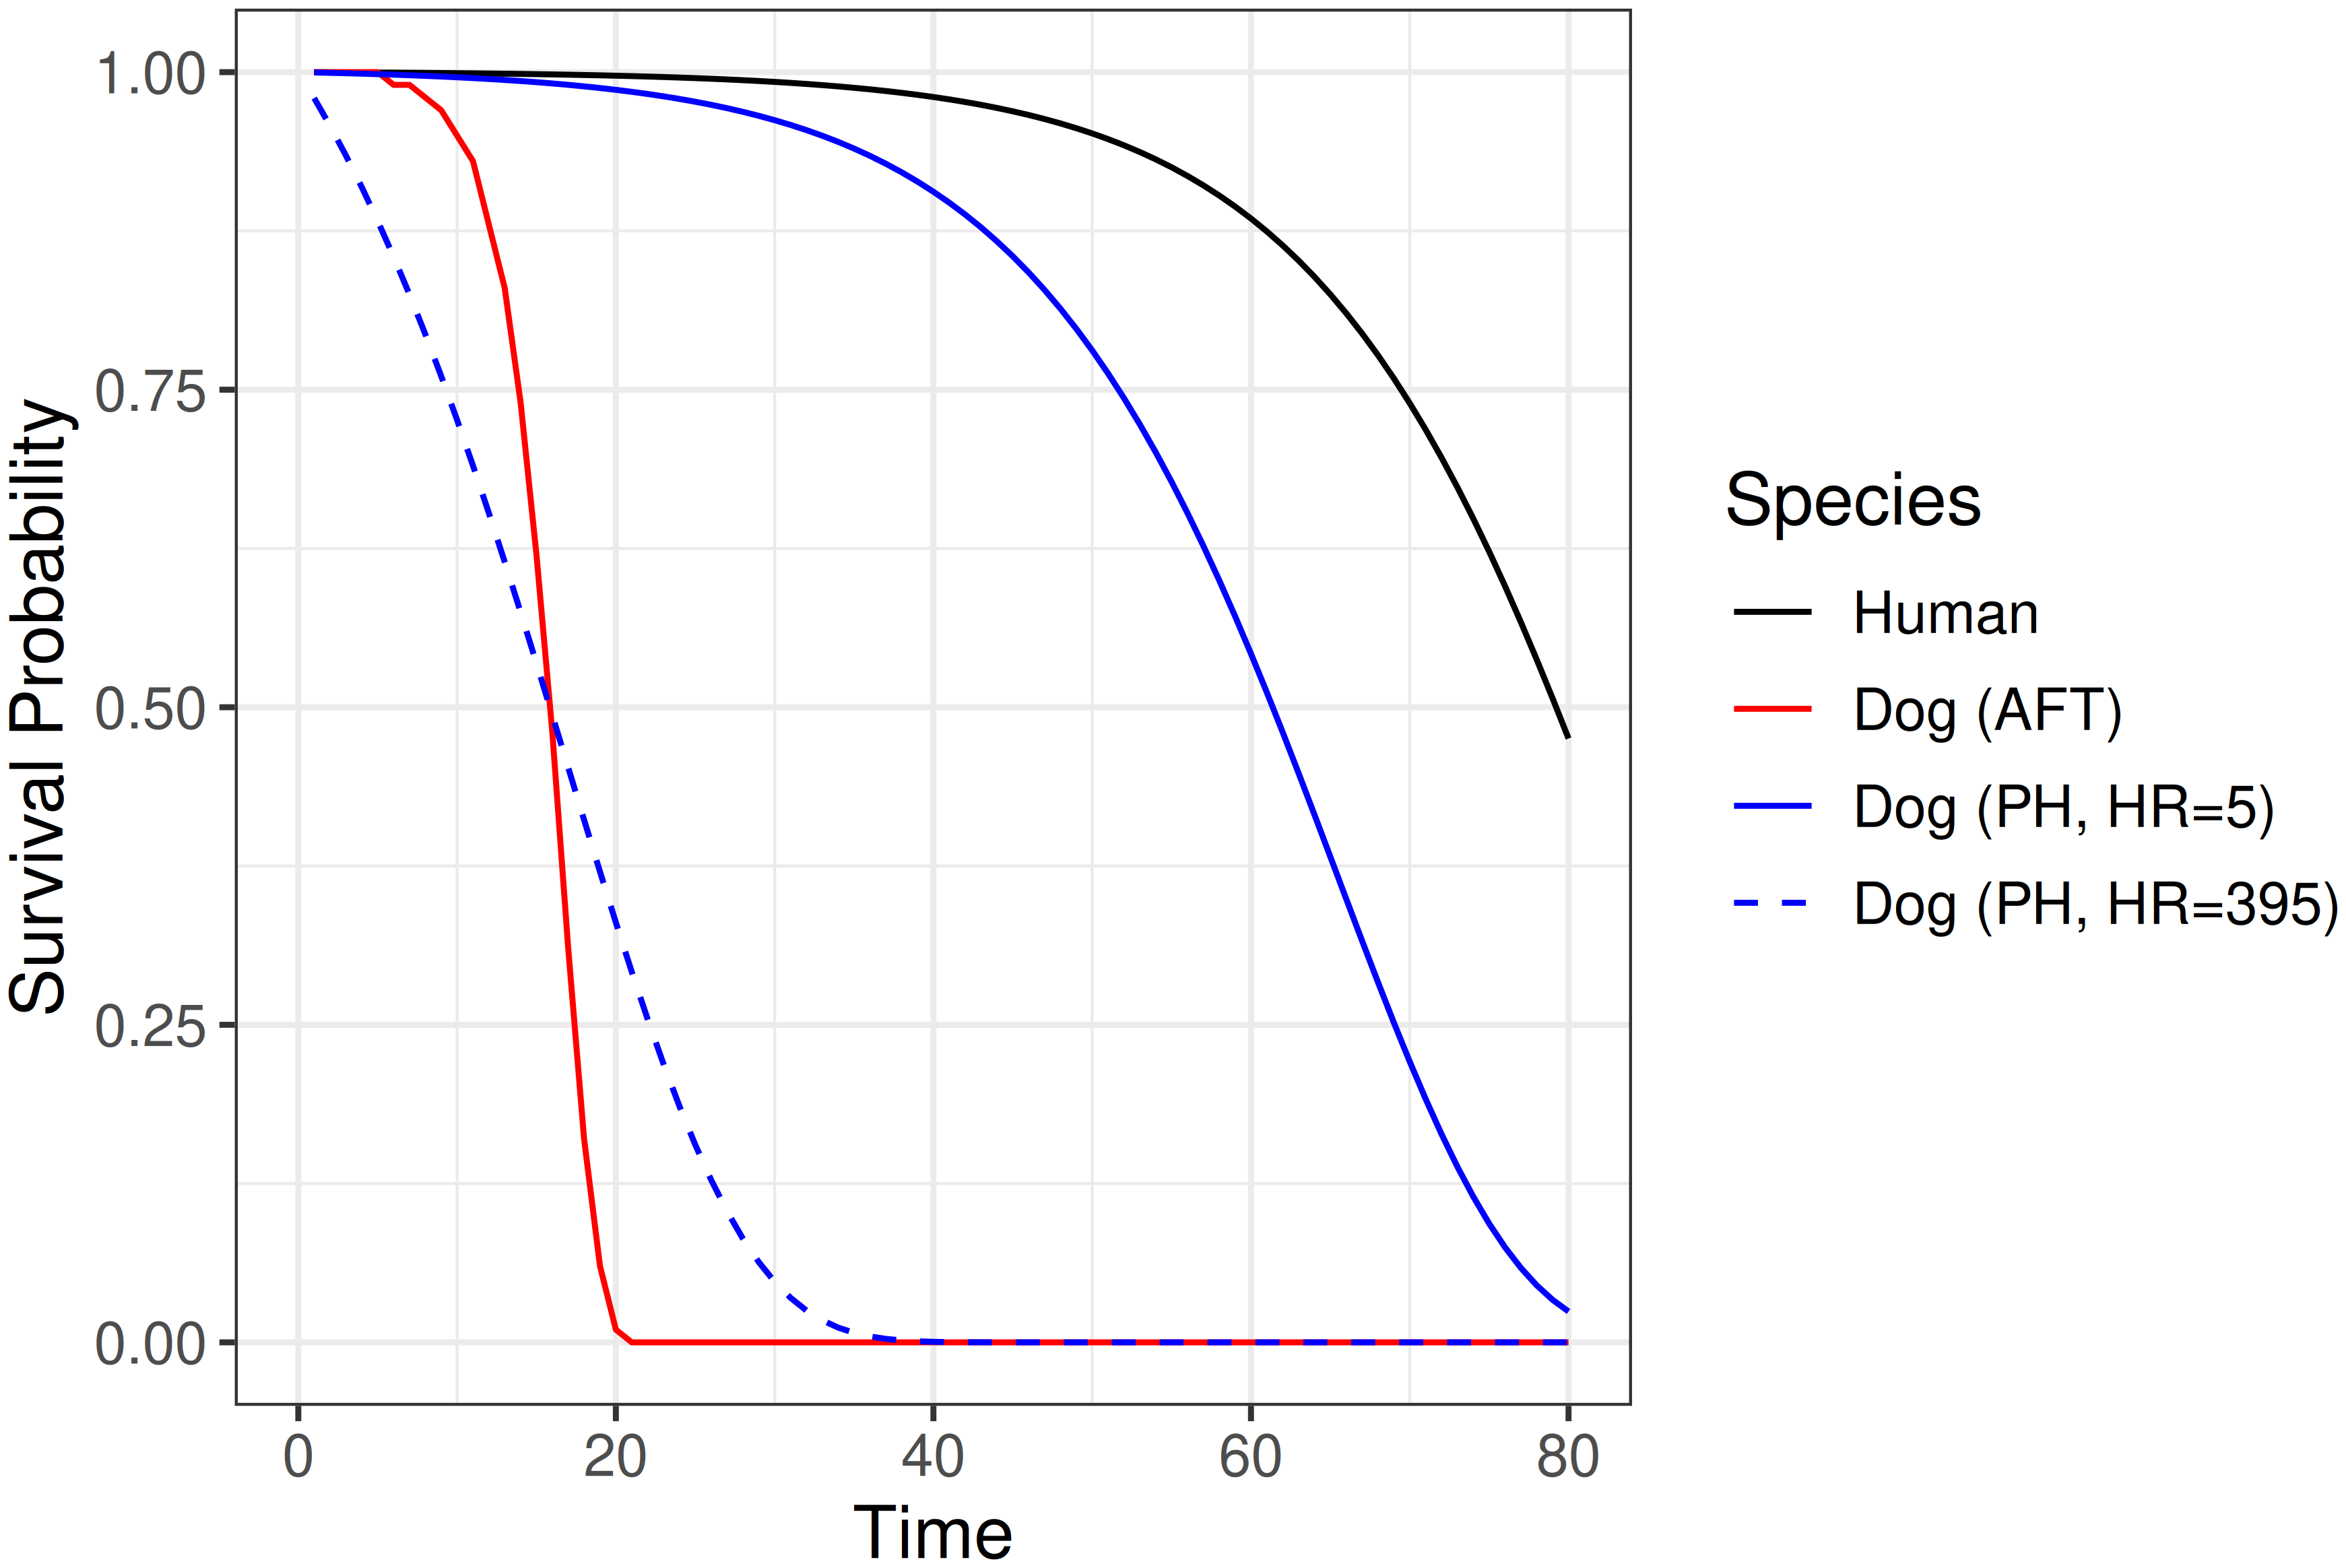
\includegraphics[width=0.7\linewidth,height=\textheight,keepaspectratio]{Figures/classical/fig-p3c13-dogs.png}

}

\caption{\label{fig-p3c13-dogs}Comparing human (black) and dog
lifespans, with the dog modeled by an AFT model (red, a five-fold
acceleration of time) and PH models (blue). The solid blue curve uses a
hazard ratio of \(5\) (the same numerical factor as the AFT
acceleration); the dashed blue curve uses the much larger hazard ratio
(\(\approx 395\)) needed to match the AFT dog's median survival, yet
still cannot reproduce its shape. Human lifespan modeled with
Gompertz(shape=0.09, rate=0.00005).}

\end{figure}%

More generally, the accelerated failure time model estimates survival
functions as:\index{accelerated failure time}

\begin{equation}\phantomsection\label{eq-aft-surv}{
S_{AFT}(\tau \mid \mathbf{x}_i) = S_0(\tau e^{-\eta_i}),
}\end{equation}

with respective hazard function:

\begin{equation}\phantomsection\label{eq-aft-haz}{
h_{AFT}(\tau \mid \mathbf{x}_i) = e^{-\eta_i} h_0(\tau e^{-\eta_i}).
}\end{equation}

where \(\eta_i = \mathbf{x}_i^\top\boldsymbol{\beta}\) is the linear
predictor for observation \(i\) (as before), and \(S_0\) and \(h_0\) are
the baseline survival and hazard functions.

Note three key differences compared to the PH model.

\begin{enumerate}
\def\labelenumi{\arabic{enumi}.}
\tightlist
\item
  \(\exp(-\eta_i)\) is modeled instead of \(\exp(\eta_i)\), which means
  the linear predictor relates to risk in the opposite direction to the
  PH model. As \(\eta_i\) increases, the inner expression of
  (\ref{eq-aft-surv}), \(\tau e^{-\eta_i}\), tends to zero and as
  \(S_0\) is a decreasing function, it follows that
  \(S_0(\tau e^{-\eta_i})\) tends to one. In a PH model, a larger
  \(\eta_i\) raises the hazard, reducing survival. Interpreting the AFT
  linear predictor as a risk score therefore reverses the book's `high
  value, high risk' convention, so its sign should be flipped before
  being used for relative-risk prediction.
\item
  The baseline risk now clearly depends on both the linear predictor as
  well as time.
\item
  An increase in a covariate results in a multiplicative effect on
  survival time, rather than the multiplicative effect on hazard seen in
  a PH model. This is often viewed as an advantage of AFT models as
  survival times may be simpler to interpret than hazard ratios.
\end{enumerate}

This third point is visualized in Figure~\ref{fig-p3c13-ph-vs-aft} in
which the linear predictor is increased by \(\log(2)\) for a PH model
and decreased by \(\log(2)\) for an AFT model. The left panel shows that
the estimated hazard function from a PH model is double the baseline at
all time points --- the multiplicative effect is seen on the y-axis
(risk). In contrast, the right panel shows how the survival function
from an AFT model decreases at double the speed to the baseline --- the
multiplicative effect is now on the x-axis (time).

\begin{figure}

\centering{

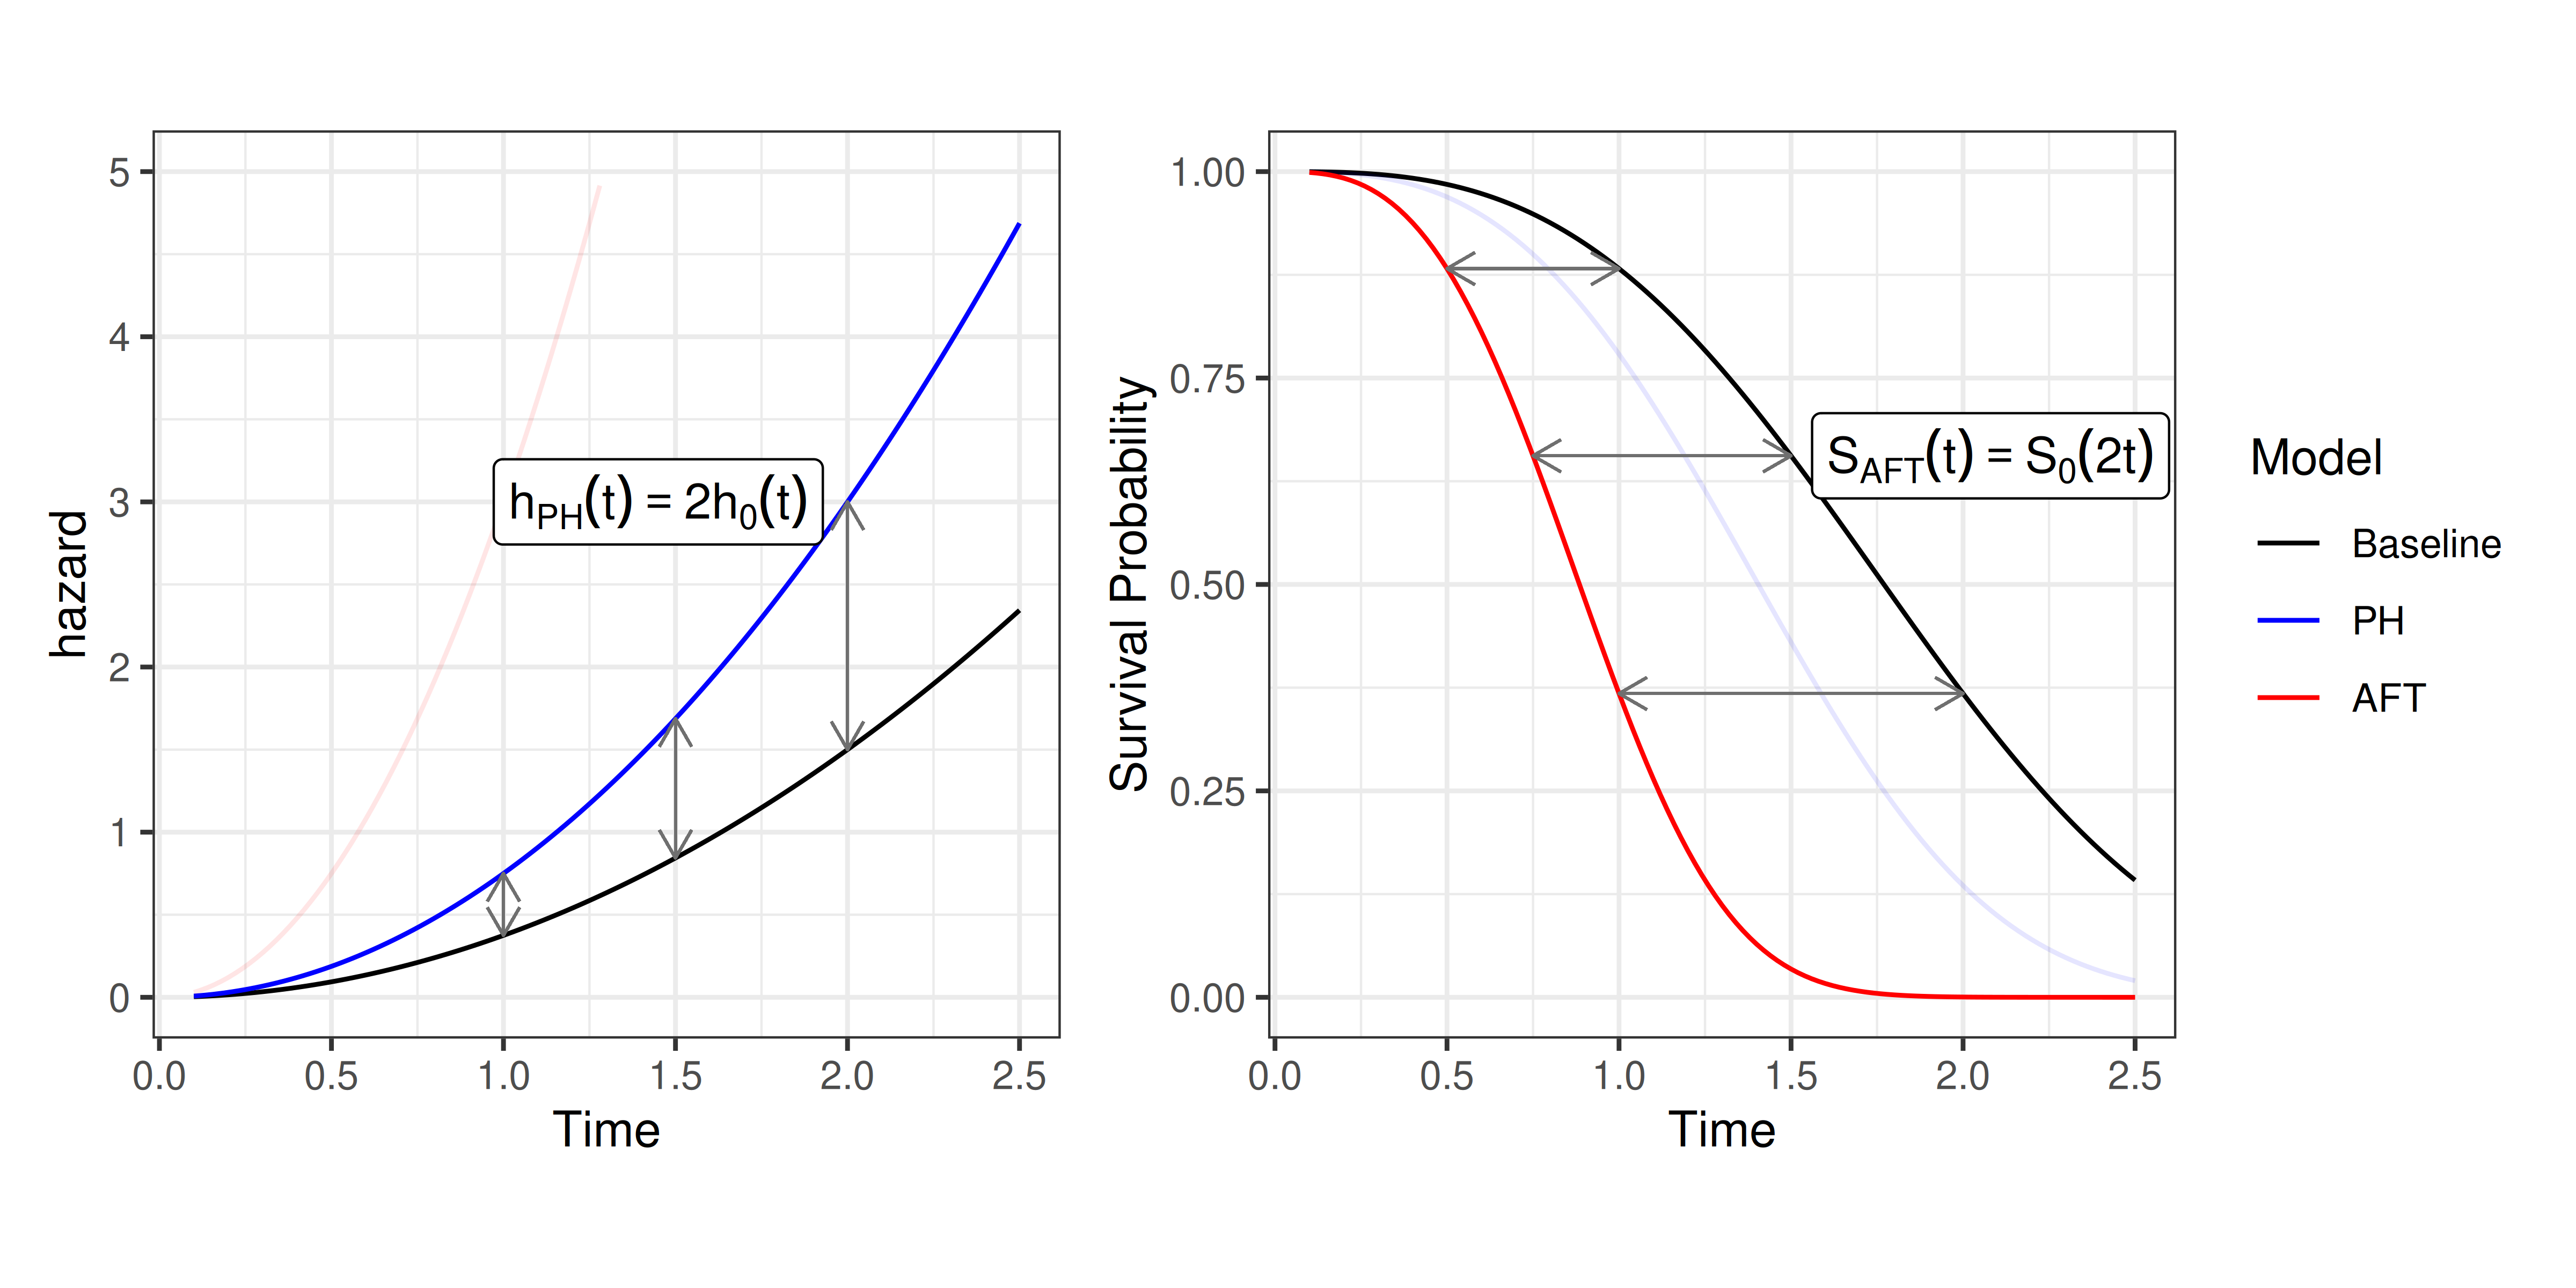
\includegraphics[width=0.9\linewidth,height=\textheight,keepaspectratio]{Figures/classical/fig-p3c13-ph-vs-aft.png}

}

\caption{\label{fig-p3c13-ph-vs-aft}Comparing changes in the linear
predictor between PH (left) and AFT (right) models. A linear predictor
increase of \(\log(2)\) multiplies \(h(\tau)\) by \(\exp(\log(2)) = 2\)
in a PH model. A linear predictor decrease of \(\log(2)\) in the AFT
results in multiplying \(\tau\) within the baseline survival by \(2\),
hence for any \(\tau\), the AFT model reaches \(S(\tau)\) in half the
time as the baseline.}

\end{figure}%

Another way to demonstrate this effect is through the log-linear form of
the accelerated failure time
model:\index{accelerated failure time!log-linear}

\begin{equation}\phantomsection\label{eq-aft-log}{
\log(\tau) = \mu + \eta + \sigma\epsilon,
}\end{equation}

where \(\sigma\) is a scale parameter, \(\epsilon\) is an error term,
and \(\mu\) is an intercept. Now consider the difference in \(\tau\)
when \(x\) is increased by one (assuming just one covariate):

\[
\log(\tau \mid x + 1) - \log(\tau \mid x) = (\mu + \beta (x + 1) + \sigma\epsilon) - (\mu + \beta x + \sigma\epsilon) = \beta,
\]

and taking exponentials of both sides gives,

\[
\frac{\tau \mid x + 1}{\tau \mid x} = \exp(\beta),
\]

showing that increasing a covariate by one unit multiplies the modeled
event time by \(\exp(\beta)\), with positive \(\beta\) corresponding to
longer survival times.

\subsection{Parametric AFTs}\label{parametric-afts}

As stated, AFTs are usually fully parametric, which means \(S_0\) and
\(h_0\) are chosen according to a specific distribution. Common
distribution choices include Weibull, exponential, log-logistic, and
log-normal (John D. Kalbfleisch and Prentice 1980; P. Wang, Li, and
Reddy 2019).
\index{Weibull distribution}\index{exponential distribution}\index{log-logistic distribution}\index{log-normal distribution}
The Weibull distribution, with the exponential distribution as a special
case, is unique as it can be parameterized as either a PH model or an
AFT model. By contrast, the log-logistic and log-normal distributions
are commonly used as AFT models but do not imply PH covariate effects.
For example, Figure~\ref{fig-p3c13-loglogistic-hazard} visualizes the
hazard function of the log-logistic distribution, which can be
non-monotonic and allows the baseline risk of an event to increase
before decreasing. When the chosen distribution is well specified, AFTs
can provide a useful alternative to PH models, especially when covariate
effects are more naturally interpreted as time ratios than hazard ratios
(Patel, Kay, and Rowell 2006; J. Qi 2009; Zare et al. 2015).

\begin{figure}

\centering{


\includegraphics[width=0.7\linewidth,height=\textheight,keepaspectratio]{Figures/classical/fig-p3c13-loglogistic-hazard.png}

}

\caption{\label{fig-p3c13-loglogistic-hazard}Log-logistic hazard curves
with a fixed scale parameter of 1 and a changing shape parameter. x-axis
is time and y-axis is the log-logistic hazard as a function of time.}

\end{figure}%

As with the PH model, AFT models can be fit using maximum likelihood
estimation of the full-likelihood
(Section~\ref{sec-surv-estimation-param}) by plugging
distribution-defining functions into
(\ref{eq-aft-surv})-(\ref{eq-aft-haz}). Using the exponential
distribution as an example, first recall that if
\(Y \sim \operatorname{Exp}(\lambda)\) then,

\[
h_Y(\tau) = \lambda \quad \text{and} \quad S_Y(\tau) = \exp(-\lambda\tau).
\]

Giving the Exponential-AFT survival and hazard functions:
\index{accelerated failure time!exponential}

\[
S_{ExpAFT}(\tau \mid \mathbf{x}_i)= \exp(-\lambda\tau e^{-\eta_i}) \quad \text{and} \quad h_{ExpAFT}(\tau \mid \mathbf{x}_i)= \lambda e^{-\eta_i}.
\]

The Exponential-AFT right-censored likelihood follows from
(\ref{eq-right-censoring-likelihood}):

\[
\begin{aligned}
\mathcal{L}(\boldsymbol{\theta}) &= \prod_{i=1}^n h_Y(t_i \mid \boldsymbol{\theta})^{\delta_i}S_Y(t_i \mid \boldsymbol{\theta}) \\
&= \prod_{i=1}^n \Big(\lambda e^{-\eta_i}\Big)^{\delta_i}\Big(\exp(-\lambda t_i e^{-\eta_i})\Big) \\
&= \prod_{i=1}^n \lambda^{\delta_i} \exp(-\lambda t_i e^{-\eta_i} - \delta_i\eta_i), \\
\end{aligned}
\]

with log-likelihood,

\[
\begin{aligned}
\ell(\boldsymbol{\theta}) &= \sum_{i=1}^n \log(\lambda^{\delta_i} \exp(-\lambda t_i e^{-\eta_i} - \delta_i\eta_i)) \\
&= \sum_{i=1}^n \delta_i\log(\lambda) - \lambda t_i e^{-\eta_i} - \delta_i\eta_i,
\end{aligned}
\]

and extensions to other censoring types and truncation follow by
specifying the correct likelihood form in
Section~\ref{sec-surv-estimation-param}.

\section{Proportional odds}\label{sec-proportionalodds}

Proportional odds (PO) models (Bennett 1983) are the final of the three
major linear model classes in survival analysis.
\index{proportional odds} In contrast to the PH and AFT models just
discussed, proportional odds models are used less widely. They are
discussed in more detail in flexible parametric models
(Section~\ref{sec-flexible}). \index{flexible parametric models} This
section briefly describes the motivation for the model and its key
properties.

As the name may suggest, the proportional odds model is analogous to the
proportional hazards model except with the goal of modeling odds instead
of hazards. In general, let \(p\) be the probability of an event
occurring, then the \emph{odds} of the event are: \index{odds}

\[
O(p) = \frac{p}{1 - p}.
\]

In a survival analysis context, the odds are calculated for the survival
probability:

\[
O(S(\tau)) = \frac{S(\tau)}{1-S(\tau)} = \frac{S(\tau)}{F(\tau)}.
\]

The PO model follows similarly to the PH model, substituting odds in
place of the hazards:

\[
O_{PO}(\tau \mid \mathbf{x}_i) =  O_0(\tau)\exp(\eta_i)
\]

where \(O_0\) is the baseline odds. A log-logistic distribution is often
assumed for the baseline odds and the model is fit by maximum likelihood
estimation on the full likelihood (Bennett 1983), discussed further in
the next section.\index{maximum likelihood estimator}

By the same logic as the proportional hazards model, this model assumes
\(O(\tau \mid \mathbf{x}_i) \propto \exp(\eta_i)\). For a model with
single covariate \(x\) and coefficient \(\beta\), by analogous maths to
(\ref{eq-ph-hazard-ratio}), a unit increase in \(x\), multiplies the
odds of surviving past \(\tau\) by \(\exp(\beta)\).

A useful implication of the PO model is the convergence of hazard
functions, which states
\(h_{PO}(\tau \mid \mathbf{x}_i)/h_0(\tau) \rightarrow 1\) as
\(\tau \rightarrow \infty\) (Kirmani and Gupta 2001). To see this, note
that the PO model can be represented in terms of the hazard function via
(Collett 2014):

\begin{equation}\phantomsection\label{eq-po}{
h_{PO}(\tau \mid \mathbf{x}_i) =  \frac{h_0(\tau)}{1 + \Big(S_0(\tau)(\exp(\eta_i) - 1)\Big)}.
}\end{equation}

Dividing by the baseline hazard,

\begin{equation}\phantomsection\label{eq-po-ratio}{
\frac{h_{PO}(\tau \mid \mathbf{x}_i)}{h_0(\tau)} = \frac{1}{1 + \Big(S_0(\tau)(\exp(\eta_i) - 1)\Big)},
}\end{equation}

and as \(\tau \rightarrow \infty\), it holds that
\(S_0(\tau) \rightarrow 0\) and (\ref{eq-po-ratio}) \(\rightarrow 1\).
As such, every individual's hazard approaches the baseline hazard over a
long period of time. This assumption holds in several contexts, most
commonly in medical domains where death is the event of interest. For
example, take two patients with a disease, patient \(i\) receives
treatment and patient \(j\) does not. Let \(\exp(\eta_i) = 4\) and
\(\exp(\eta_j) = 1\) be their respective survival odds ratios (relative
to baseline) and let \(S_0(0) = 1\) and \(S_0(5) = 0.01\) be baseline
survival at times \(0\) and \(5\). Following (\ref{eq-po}), for patient
\(i\):

\[
h_{PO}(0 \mid \mathbf{x}_i) =  0.25h_0(0); \quad\quad h_{PO}(5 \mid \mathbf{x}_i) =  0.97h_0(5),
\]

and for patient \(j\):

\[
h_{PO}(0 \mid \mathbf{x}_j) = h_0(0); \quad\quad h_{PO}(5 \mid \mathbf{x}_j) = h_0(5).
\]

The treatment effect reduces the hazard for observation \(i\) at early
time points. However, at the later time point, the hazard is similar for
both observations. This example highlights a similarity to AFT models
(Section~\ref{sec-surv-models-param}): under the survival-odds
parameterization, larger values of \(\eta\) decrease the hazard.
Therefore, once again, care must be taken when using these models for
relative risk predictions to ensure a consistent interpretation of risk.

\section{Flexible parametric models}\label{sec-flexible}

Royston-Parmar flexible parametric models (Royston and Parmar 2002)
extend PH and PO models by estimating the baseline hazard with natural
cubic splines. \index{flexible parametric models} The model was designed
to keep the form of the PH or PO methods but without estimating a
potentially misleading baseline hazard (for semi-parametric models) or
misspecifying the survival distribution (for fully-parametric models).
Although the Royston-Parmar model is not a core model in the same sense
as the Cox proportional hazards or accelerated failure time models, it
naturally belongs here as it is a straightforward combination of core
models and methods (Section~\ref{sec-classical-improving}).

The crux of the method is to use splines to model time on a log-scale
and to either estimate the log cumulative hazard for PH models, or the
log odds for PO models. For the flexible PH model, a Weibull
distribution is the basis for the baseline distribution, whereas a
log-logistic distribution is assumed for the baseline odds in the
flexible PO model.
\index{proportional hazards}\index{proportional odds}\index{Weibull distribution}\index{log-logistic distribution}
A recommended summary of the model is given in Collett (2014).

The flexible parametric Royston-Parmar (RP) proportional hazards and
proportional odds model are respectively defined by:

\begin{equation}\phantomsection\label{eq-rp-hazard}{
\log{H}_{RP}(\tau \mid \mathbf{x}_i) = s(\tau \mid \boldsymbol{\nu},\mathbf{k}) + \eta_i,
}\end{equation}

and

\begin{equation}\phantomsection\label{eq-rp-odds}{
\log{O}_{RP}(\tau \mid \mathbf{x}_i) = s(\tau \mid \boldsymbol{\nu},\mathbf{k}) + \eta_i,
}\end{equation}

where \(\boldsymbol{\nu}\) are spline coefficients to be fitted by
maximum likelihood estimation, \(\mathbf{k}\) are the positions of \(K\)
internal knots, and \(s\) is the restricted cubic spline function in log
time defined by, \index{splines}

\[
s(\tau \mid \boldsymbol{\nu},\mathbf{k}) = \nu_0 + \nu_1\log(\tau) + \nu_2 B_1(\log(\tau)) + \ldots + \nu_{K+1} B_K(\log(\tau)),
\]

\(B_j\) is the basis function at knot \(k_j\) defined
by,\index{basis functions}

\[
B_j(x) = (x - k_j)^3_+ - \omega_j(x - k_{min})^3_+ - (1 - \omega_j)(x - k_{max})^3_+,
\]

where the weight \(\omega_j\), determined entirely by the knot
locations, is chosen so that \(B_j\) is linear beyond the boundary
knots,

\[
\omega_j = \frac{k_{max} - k_j}{k_{max} - k_{min}},
\]

and \((x - y)_+ = \max\{0, (x - y)\}\) for any \(x, y\), and where
\(k_{min}\) and \(k_{max}\) are the boundaries of the cubic spline,
meaning the curve is linear when \(\log(t) < k_{min}\) or
\(\log(t) > k_{max}\).

To see how the proportional hazards RP model relates to the Weibull
distribution, first integrate and take logs of the Weibull-PH hazard
function from (\ref{eq-ph-weibull-haz}):
\index{proportional hazards!Weibull}

\[
\log(H_{WeibullPH}(\tau \mid \mathbf{x}_i)) = \log\big((\lambda \tau^\gamma) \exp(\eta_i)\big) = \log(\lambda) + \gamma\log(\tau) + \eta_i
\]

Setting \(\nu_0 = \log(\lambda)\) and \(\nu_1 = \gamma\) yields
(\ref{eq-rp-hazard}) when there are no knots. Analogous results can be
shown between (\ref{eq-rp-odds}) and the log-logistic distribution.

To fit the model, the number and position of knots are theoretically
tunable, although Royston and Parmar advised against tuning and suggest
often only one internal knot is required and the placement of the knot
does not make a significant difference to performance (Royston and
Parmar 2002). \index{hyperparameter optimization} While increasing knots
can increase model overfitting, Bower et al. (2019) showed up to seven
knots does not significantly increase model bias. The model's primary
advantage is its flexibility to model non-linear effects (see also
Section~\ref{sec-nonlinear}) and can also be extended to time-dependent
covariates. The Royston-Parmar model can be fit by maximum likelihood
estimation, making estimation of smooth survival functions under this
framework straightforward using readily available off-the-shelf
software.

In the same manner as other proportional hazards models, the
Royston-Parmar model can be extended to competing risks by modeling
cause-specific hazards, considering only one event at a time and
censoring competing events (Hinchliffe and Lambert 2013).

\section{Core methods}\label{sec-classical-improving}

A number of model-agnostic algorithms have been created to improve a
model's predictive ability. Such extensions of the above models can lead
to substantial performance improvements. These are referred to as `core
methods'. Like the core models, they are pervasive in the literature and
are often found as components within more complex alternatives.

Three extensions are discussed briefly:

\begin{enumerate}
\def\labelenumi{\arabic{enumi}.}
\tightlist
\item
  modeling non-linear feature effects;
\item
  reducing the number of variables used by the model, either by feature
  selection or by shrinking their effects toward zero; and
\item
  combining predictions from multiple models.
\end{enumerate}

\subsection{Non-linear effects}\label{sec-nonlinear}

One of the major limitations of the models discussed so far is the
assumption of a linear relationship between covariates and outcomes (on
the scale of the predictor). At first, one might view the Cox model as
non-linear due to the presence of the exponential function. However, the
linearity becomes clear when the model is written in terms of its linear
predictor \(\eta\): \index{non-linear effects}

\[
\eta = x_1\beta_1 + \ldots + x_p\beta_p.
\]

Consider modeling the time until disease progression with covariates
representing age (continuous) and treatment (binary):

\[
\eta = x_{age}\beta_{age} + x_{trt}\beta_{trt}.
\]

In this form, increasing age from \(1\) to \(21\) or \(81\) to \(101\)
has the same effect on the linear predictor \(\eta\); this is clearly
not realistic. There are many approaches to relaxing linearity; these
are discussed extensively elsewhere and not repeated here, James et al.
(2013) covers non-linear modeling in detail.

In brief, the models discussed in this chapter can be extended to
\emph{additive models} in the same manner as a regression model.
\index{additive model} For example,

\[
\eta = f_1(x_1) + \ldots + f_p(x_p),
\]

where each \(f_j\) is a smooth, possibly non-linear function of its
covariate. If all \(f_j\) are linear functions then this recovers the
standard linear predictor \(\eta = x_1\beta_1 + \ldots + x_p\beta_p\).

In practice, each \(f_j\) is represented as a linear combination of
\(M_j\) known basis functions,\index{basis functions}

\[
f_j(x_j) = \sum_{m=1}^{M_j} \nu_{jm} B_{jm}(x_j),
\]

where \(B_{jm}\) are the basis functions and the \(\nu_{jm}\) are the
corresponding basis coefficients to be estimated. Many basis systems can
be used, including natural cubic splines, B-splines and the closely
related penalized B-splines (P-splines) (Eilers and Marx 1996), and
thin-plate regression splines (Wood 2003); simpler choices such as step
functions or polynomial bases are also possible (see Wood (2017) for a
comprehensive treatment of spline-based
modeling).\index{splines}\index{penalization}

Highly flexible basis functions can easily overfit the data, so
estimation is usually combined with a penalty on the basis coefficients.
Collecting all parameters in \(\boldsymbol{\theta}\), the functions are
estimated by optimizing a penalized criterion of the general form

\[
L(\boldsymbol{\theta}) + \xi P(\boldsymbol{\theta}),
\]

where \(L(\boldsymbol{\theta})\) is a loss function, typically the
negative log-likelihood, \(P(\boldsymbol{\theta})\) is a penalty on the
basis coefficients, and \(\xi \geq 0\) is a tuning parameter governing
the trade-off between goodness-of-fit and smoothness. For a single
function \(f_j\), a common penalty is the sum of squared differences
between adjacent coefficients (Eilers and Marx 1996),

\[
P(\boldsymbol{\theta}) = \sum_{m=2}^{M_j} (\nu_{jm} - \nu_{j,m-1})^2,
\]

which shrinks neighboring coefficients towards one another and thereby
penalizes abrupt changes in \(f_j\). As \(\xi \to 0\), the estimate
approaches the unpenalized fit, whereas a large \(\xi\) forces each
\(f_j\) towards a flatter function. Flexible parametric models like the
Royston-Parmar model (Section~\ref{sec-flexible}) are additive models
that use splines to model the baseline hazard, and are implemented in
the \texttt{flexsurv} package (Jackson 2016). Additive Cox models, which
instead estimate smooth functions of the covariates directly within the
proportional hazards framework, are described in Hastie and Tibshirani
(1990).

The constructions above make the predictor considerably more flexible,
but they still assume that each effect is a smooth function of a single
covariate, rule out interactions between covariates, and require advance
specification of which features are modeled using splines and how. More
generally, the predictor can be written as

\[
y = g(\mathbf{x}\mid \boldsymbol{\theta}) = r(\eta(\mathbf{x}\mid \boldsymbol{\theta})),
\]

where \(\boldsymbol{\theta}\) collects all parameters of the model and
\(g\) is a general function of the features that may include non-linear
effects, interactions, and non-smooth components, and \(r\) is a
response function\index{response function} that maps the predictor
\(\eta\) to the target space. Machine learning models, including all
those discussed in the next chapters, are designed to learn such
functions directly from data, without the need to pre-specify the range
of possible effects.

\subsection{Dimension reduction and feature
selection}\label{dimension-reduction-and-feature-selection}

In many high-dimensional predictive modeling problems, only a small
subset of variables in datasets tend to be relevant for correctly
predicting the outcome. Other variables are either redundant, providing
no more information than their counterparts, or irrelevant, they do not
influence the outcome. In these cases, using all variables for modeling
results in worse interpretability, increased computational complexity,
and often inferior model performance as models tend to overfit the
training data and generalize poorly to new data.

To improve model performance, one can therefore apply feature selection
methods to reduce the number of variables the model uses.
\index{feature selection}\index{dimension reduction} Feature selection
is often grouped into three categories: 1) wrappers; 2) embedded
methods; and 3) filters. Wrappers fit multiple models on subsets of
variables and select the best-performing subsets. This is often
computationally infeasible in the context of very large datasets. This
section does not consider general algorithms such as principal component
analysis, see further reading below for suggested material that covers
these areas.

\subsubsection{Embedded methods}\label{embedded-methods}

Embedded methods refer to those that are incorporated during model
fitting. Many machine learning models incorporate embedded methods and
thus reduce the number of variables the model relies on as part of the
training process. Models that do not apply feature selection during
training tend to perform poorly when there is a large number of
variables in a dataset. One model that straddles the line between core
modeling and machine learning methodology is the elastic Cox model,
which incorporates the lasso and ridge regularization methods. Given a
generic learning algorithm, lasso and ridge regularization constrain the
model coefficients subject to the \(\ell^1\)-norm and \(\ell^2\)-norm
respectively. The Lasso-Cox (Tibshirani 1997) model fits the Cox model
\index{Cox proportional hazards} by estimating \(\boldsymbol{\beta}\)
as: \index{Cox proportional hazards!lasso}\index{lasso}

\[
\hat{\boldsymbol{\beta}} = \mathop{\mathrm{arg\,max}}\mathcal{L}(\boldsymbol{\beta}); \text{ subject to } \sum \vert \beta_j \vert \leq \gamma,
\]

where \(\mathcal{L}\) is the likelihood defined in (\ref{eq-partial})
and \(\gamma > 0\) is a hyperparameter.

In contrast, the Ridge-Cox model estimates \(\boldsymbol{\beta}\) as:
\index{Cox proportional hazards!ridge}\index{ridge}

\[
\hat{\boldsymbol{\beta}} = \mathop{\mathrm{arg\,max}}\ \mathcal{L}(\boldsymbol{\beta}); \text{ subject to } \sum \beta_j^2 \leq \gamma.
\]

Lasso and ridge are both shrinkage methods, which are used to reduce
model variance and overfitting, especially in the context of
multicollinearity. However, the \(\ell^1\) norm in Lasso regression can
also shrink coefficients to zero and thus performs variable selection as
well. One could perform feature selection and then pass the reduced
variables to a Ridge-Cox model; however, experiments have shown
Ridge-Cox on its own is already a powerful tool (Spooner et al. 2020).
Deciding between lasso and ridge can also be automated by using elastic
net (N. Simon et al. 2011; Zou and Hastie 2005), which is a convex
combination of \(\ell^1\) and \(\ell^2\) penalties such that
\(\boldsymbol{\beta}\) is estimated as:
\index{Cox proportional hazards!elastic net}

\[
\hat{\boldsymbol{\beta}} = \mathop{\mathrm{arg\,max}}\mathcal{L}(\boldsymbol{\beta}); \text{ subject to } \alpha \sum \vert \beta_j \vert + (1-\alpha) \sum \beta_j^2 \leq \gamma,
\]

where \(\alpha\) is a hyperparameter to be tuned
(Section~\ref{sec-ml-opt}).

\subsubsection{Filter methods}\label{filter-methods}

Filter methods are a two-step process that score features according to
some metric and then select either a given number of top-performing
features (those with the top scores) or those where the score exceeds
some threshold. \index{feature selection} The number of features to
select, or the threshold to exceed, can be treated as a hyperparameter
to tune.

Bommert et al. (2021) compared 14 filter methods for high-dimensional
survival data and found that the most powerful method was a simple
variance filter:

\[
V(\mathbf{x}_{\cdot j}) = \operatorname{Var}(\mathbf{x}_{\cdot j})
\]

where \(\mathbf{x}_{\cdot j}\) is the \(j\)th variable in the data and
\(V\) is the resulting score. The filter measures the amount of variance
in the feature and removes features that have little variation.

Another common filter method is to train a model with embedded feature
selection and pass these results to a simpler model. This is
particularly useful when model interpretability is the priority. Common
choices for models to use in the first step of the pipeline include
random forests (Chapter~\ref{sec-ranfor}) and gradient boosting machines
(Chapter~\ref{sec-boost}).

\subsection{Ensemble methods}\label{ensemble-methods}

Ensemble methods fit multiple models and combine the result into a
single prediction. Common ensemble methods include boosting, bagging,
and stacking.
\index{ensemble}\index{boosting}\index{bagging}\index{stacking} These
are briefly explained below and can be applied to any model, whether
machine learning or a simple linear model. Care is needed when fitting
ensembles to avoid data leakage. In particular, stacking should use
predictions from base models that were not trained on the same
observations used to fit the meta-model.

\subsubsection{Bagging and averaging}\label{bagging-and-averaging}

The simplest ensemble method is to fit multiple models on the same data
and make predictions by taking an average over the individual model
predictions.\index{bagging} The average over predictions could be
uniform, weighted with weights selected through expert knowledge, or
weighted with weights optimized as hyperparameters. Ensemble methods
perform best when there is high variance between models as each then
captures unique information about the underlying data. Therefore,
ensemble averaging is usually used after first subsetting (without
replacement) the training data and training each model on a different
subset.

While increasing variance is beneficial, too much variance may result in
worse predictions. Hence, bagging (Bootstrap AGGregatING) is a common
approach to increase variance without losing predictive accuracy.
Bootstrapping is the process of sampling data \emph{with} replacement,
meaning the rows may be duplicated in each subset (discussed further in
Chapter~\ref{sec-ranfor}). Models are then trained on the bootstrapped
data.

\subsubsection{Model-based boosting}\label{model-based-boosting}

Model-based boosting fits a sequence of models that iteratively improve
predictive performance by correcting errors from previous
iterations.\index{boosting} The initial model is fit to the training
data and subsequent models are fit on the same features but using
pseudo-residuals as targets, resulting in a sequence of regression
tasks. These \emph{pseudo-residuals} are the negative gradient
(Section~\ref{sec-ml-gradient-descent}) of a chosen loss function
evaluated at the previous iteration; this process is revisited in detail
in Chapter~\ref{sec-boost}. \index{gradient descent}
\index{pseudo-residuals} Fitting each subsequent model to the
pseudo-residuals focuses learning on the remaining prediction error and
incrementally improves the overall ensemble. In survival analysis, many
of the losses discussed in Part II can be incorporated into this
framework, with the choice of loss depending on the prediction task of
interest. Model-based boosting is a general framework and may
underperform the purpose-built algorithms discussed in
Chapter~\ref{sec-boost}.

\subsubsection{Stacking}\label{stacking}

Stacking can improve model performance by fitting multiple models and
aggregating the predictions using a meta-model. \index{stacking} Fitting
a meta-model, often a simple linear model, results in fitted
coefficients that weight the input models according to how close or far
they were from the truth.

Training data is partitioned (once or several times) and the first
partition is used to train several independent models, a meta-model is
fit using the outputs (predictions) from the base models as features and
the targets \((t_i,\delta_i)\) from the second partition as targets.

For example, consider stacking three Cox models with a Cox meta-model.
\index{Cox proportional hazards} Let
\(\mathcal{D}= \{(\mathbf{x}_i, t_i, \delta_i)\}_{i=1}^N\) be a dataset.
Partition \(\mathcal{D}\) into two disjoint datasets: \(\mathcal{D}_1\)
of size \(n\) and \(\mathcal{D}_2\) of size \(m\). Three Cox base models
are fit on \(\mathcal{D}_1\), each using a different feature set so that
the base models are distinct, and linear predictors are predicted for
all \(m\) observations in \(\mathcal{D}_2\):

\[
\mathbf{Z} = 
\begin{bmatrix}
\hat{\eta}^{(1)}_{1} & \hat{\eta}^{(2)}_{1} & \hat{\eta}^{(3)}_{1} \\
\vdots & \vdots & \vdots \\
\hat{\eta}^{(1)}_{m} & \hat{\eta}^{(2)}_{m} & \hat{\eta}^{(3)}_{m} \\
\end{bmatrix},
\]

where \(\hat{\eta}^{(j)}_{i}\) is the linear predictor for the \(i\)th
observation in the validation set from the \(j\)th base model.

The meta-Cox model is then fit on
\(\{(\mathbf{Z}, (t_i, \delta_i)_{i \in \mathcal{D}_2})\}\):

\[
h_M(\tau \mid \hat{\boldsymbol{\eta}}_i) = h^{(M)}_{0}(\tau)\exp(\beta^{(M)}_1\hat{\eta}^{(1)}_{i} + \beta^{(M)}_2\hat{\eta}^{(2)}_{i} + \beta^{(M)}_3\hat{\eta}^{(3)}_{i}), \quad i \in \mathcal{D}_2,
\]

where \(\hat{\boldsymbol{\beta}}^{(M)}\) and \(\hat{h}^{(M)}_0\) are the
learned coefficients and baseline hazard respectively for the
meta-model. Finally, the base learners are refit on all \(\mathcal{D}\)
but keeping \(\hat{\boldsymbol{\beta}}^{(M)}\) and \(\hat{h}^{(M)}_0\)
from the meta-model fixed.

Predictions for a new observation \(\mathbf{x}_*\) are made by first
predicting
\((\mathbf{x}_*^\top\hat{\beta}^{(1)},\mathbf{x}_*^\top\hat{\beta}^{(2)},\mathbf{x}_*^\top\hat{\beta}^{(3)})\)
from the trained base models and passing those to \(h_M\) using the
fitted \(\hat{\boldsymbol{\beta}}^{(M)}\) coefficients and
\(\hat{h}^{(M)}_0\).

In the above example, Cox models are used throughout. However, any
machine learning models with the same prediction types can be stacked,
including combinations of models. One particularly popular form of
stacking in survival analysis is the \emph{SuperLearner} method (Laan,
Polley, and Hubbard 2007), which constructs an ensemble by optimally
weighting multiple candidate models based on cross-validated predictive
performance. \index{SuperLearner}

\section{Conclusion}\label{conclusion-8}

\begin{tcolorbox}[enhanced jigsaw, toprule=.15mm, bottomtitle=1mm, opacityback=0, breakable, leftrule=.75mm, title={Key takeaways}, toptitle=1mm, bottomrule=.15mm, colback=white, colframe=quarto-callout-warning-color-frame, titlerule=0mm, opacitybacktitle=0.6, coltitle=black, rightrule=.15mm, left=2mm, colbacktitle=quarto-callout-warning-color!10!white, arc=.35mm]

\begin{itemize}
\tightlist
\item
  Core statistical models broadly fall into three categories:
  non-parametric estimators, semi-parametric models that include a
  non-parametric baseline estimate, and fully-parametric models.
\item
  Non-parametric estimators are used throughout survival analysis, often
  as components in more complex machine learning models.
\item
  Proportional hazards and accelerated failure time models encode
  different assumptions but both are powerful predictive tools.
\item
  The boundary between machine learning and statistical models is fuzzy,
  and simpler survival models can outperform more complex machine
  learning alternatives (Burk et al. 2026).
\item
  Simpler (linear) models encode assumptions that are rarely met in
  practice, for example the proportional hazards assumption. However,
  even if assumptions are violated, these often still generalize well to
  new data and are worth including in benchmark experiments.
\item
  Unregularized models perform badly on high-dimensional data without
  some form of pre-processing, however this is relatively simple with
  modern software such as \texttt{sklearn} (Pedregosa et al. 2011) and
  \texttt{mlr3} (Lang et al. 2019).
\end{itemize}

\end{tcolorbox}

\begin{tcolorbox}[enhanced jigsaw, toprule=.15mm, bottomtitle=1mm, opacityback=0, breakable, leftrule=.75mm, title={Further reading}, toptitle=1mm, bottomrule=.15mm, colback=white, colframe=quarto-callout-tip-color-frame, titlerule=0mm, opacitybacktitle=0.6, coltitle=black, rightrule=.15mm, left=2mm, colbacktitle=quarto-callout-tip-color!10!white, arc=.35mm]

\begin{itemize}
\tightlist
\item
  To learn more about hazard ratios from Cox models and complexities in
  interpretation, see Sashegyi and Ferry (2017) and Spruance et al.
  (2004).
\item
  Extensions of the proportional hazards framework include more general
  hazard-based models that allow covariates to act simultaneously on the
  hazard and time scales. An example is the general hazards model of (Y.
  Q. Chen and Jewell 2001). While flexible, such models do not appear
  common in predictive modeling but are instead preferred for inference
  (for example, Francisco J. Rubio et al. 2019; Francisco Javier Rubio
  and Drikvandi 2022; Tong et al. 2013).
\item
  Collett (2014) and John D. Kalbfleisch and Prentice (1980) both
  provide comprehensive reading for core statistical models. The former
  is slightly less technical and covers extensions to multiple settings.
\item
  For more abstract feature selection algorithms that can be applied to
  any data (survival or otherwise), see Chandrashekar and Sahin (2014)
  and Guyon and Elisseeff (2003).
\item
  Kernel-based approaches not covered here have been suggested for
  smooth non-parametric estimates of the baseline hazard (Gefeller and
  Dette 1992; Müller and Wang 1994).
\end{itemize}

\end{tcolorbox}

\chapter{Random Forests}\label{sec-ranfor}

Random forests are a composite (or ensemble)
algorithm\index{ensemble}\index{random forests} built by fitting many
simpler component models, decision trees, and then averaging their
predictions.\index{decision tree} Due to their built-in feature
selection capabilities, random forests are commonly used in
high-dimensional settings when the number of variables far exceeds the
number of observations
(rows).\index{feature selection}\index{high-dimensional data} Despite
being black boxes, especially as the number of trees increases, random
forests have natural feature importance measures which make them one of
the more interpretable machine learning
algorithms.\index{feature importance}\index{interpretable machine learning}
Random survival forests therefore remain a popular and well-performing
model in the survival setting, both for predictive modeling and pattern
recognition.\index{random survival forests}

\section{Random forests for
regression}\label{random-forests-for-regression}

Training of decision trees can include a large number of hyperparameters
and different training steps including `growing' and subsequently
`pruning'.\index{decision tree} However, when utilized in random
forests, many of these parameters and steps can be safely ignored, hence
this section only focuses on the components that primarily influence the
resulting random forest. This section will start by discussing decision
trees and will then introduce the \emph{bagging} algorithm used to
create random forests.\index{bagging}

\subsection{Decision trees}\label{decision-trees}

\emph{Decision trees} are machine learning models that are comparatively
simple to implement in software and are highly
interpretable.\index{decision tree} A decision tree algorithm takes a
dataset as input and partitions the data into distinct, non-overlapping
subsets known as \emph{nodes}. \index{random forests!node} Partitioning
is performed by applying a \emph{splitting rule} to a single feature,
creating \emph{branches} that divide the data according to a selected
cutoff or
category.\index{random forests!splitting rule}\index{random forests!branch}
This process is repeated recursively, potentially using different
features at each split, until a \emph{stopping rule} is reached. The
final nodes are referred to as \emph{terminal nodes} or
\emph{leaves}.\index{random forests!splitting rule}\index{random forests!terminal node}\index{random forests!leaf}

For example, (Figure~\ref{fig-p3c14-cars-tree}) demonstrates a decision
tree\index{decision tree} predicting the price that a car sells for in
India (price in thousands of dollars). The dataset includes as
variables: transmission type (manual or automatic), registration year,
fuel type (petrol or diesel), number of owners, kilometers driven, and
seller type. The decision tree was trained with a maximum depth of 2
(the number of rows excluding the top), and it can be seen that with
this restriction only the transmission type, registration year, and fuel
type were selected
variables.\index{random forests!hyperparameters!maximum depth} During
training, the algorithm identified that the first optimal variable to
split the data was transmission type, partitioning the data into manual
and automatic cars. Manual cars are further split by registration year
whereas automatic cars are split by fuel type. The average sale prices
in the final leaves are the terminal node predictions
(Section~\ref{sec-tree-terminal-nodes}).

The graphic highlights several core features of decision trees:

\begin{enumerate}
\def\labelenumi{\arabic{enumi}.}
\tightlist
\item
  they can model non-linear and interaction effects: The hierarchical
  structure allows for complex interactions between variables with some
  variables being used to separate all observations (transmission) and
  others only applied to subsets (year and
  fuel);\index{random forests!interactions}
\item
  they are highly interpretable: it is easy to visualize the tree and
  see how predictions are made;
\item
  they perform variable selection: not all variables were used to train
  the model.\index{random forests!variable selection}
\end{enumerate}

To understand how random forests work, it is worth looking a bit more
into the most important components of decision trees: splitting rules,
stopping rules, and terminal node predictions.

\begin{figure}

\centering{

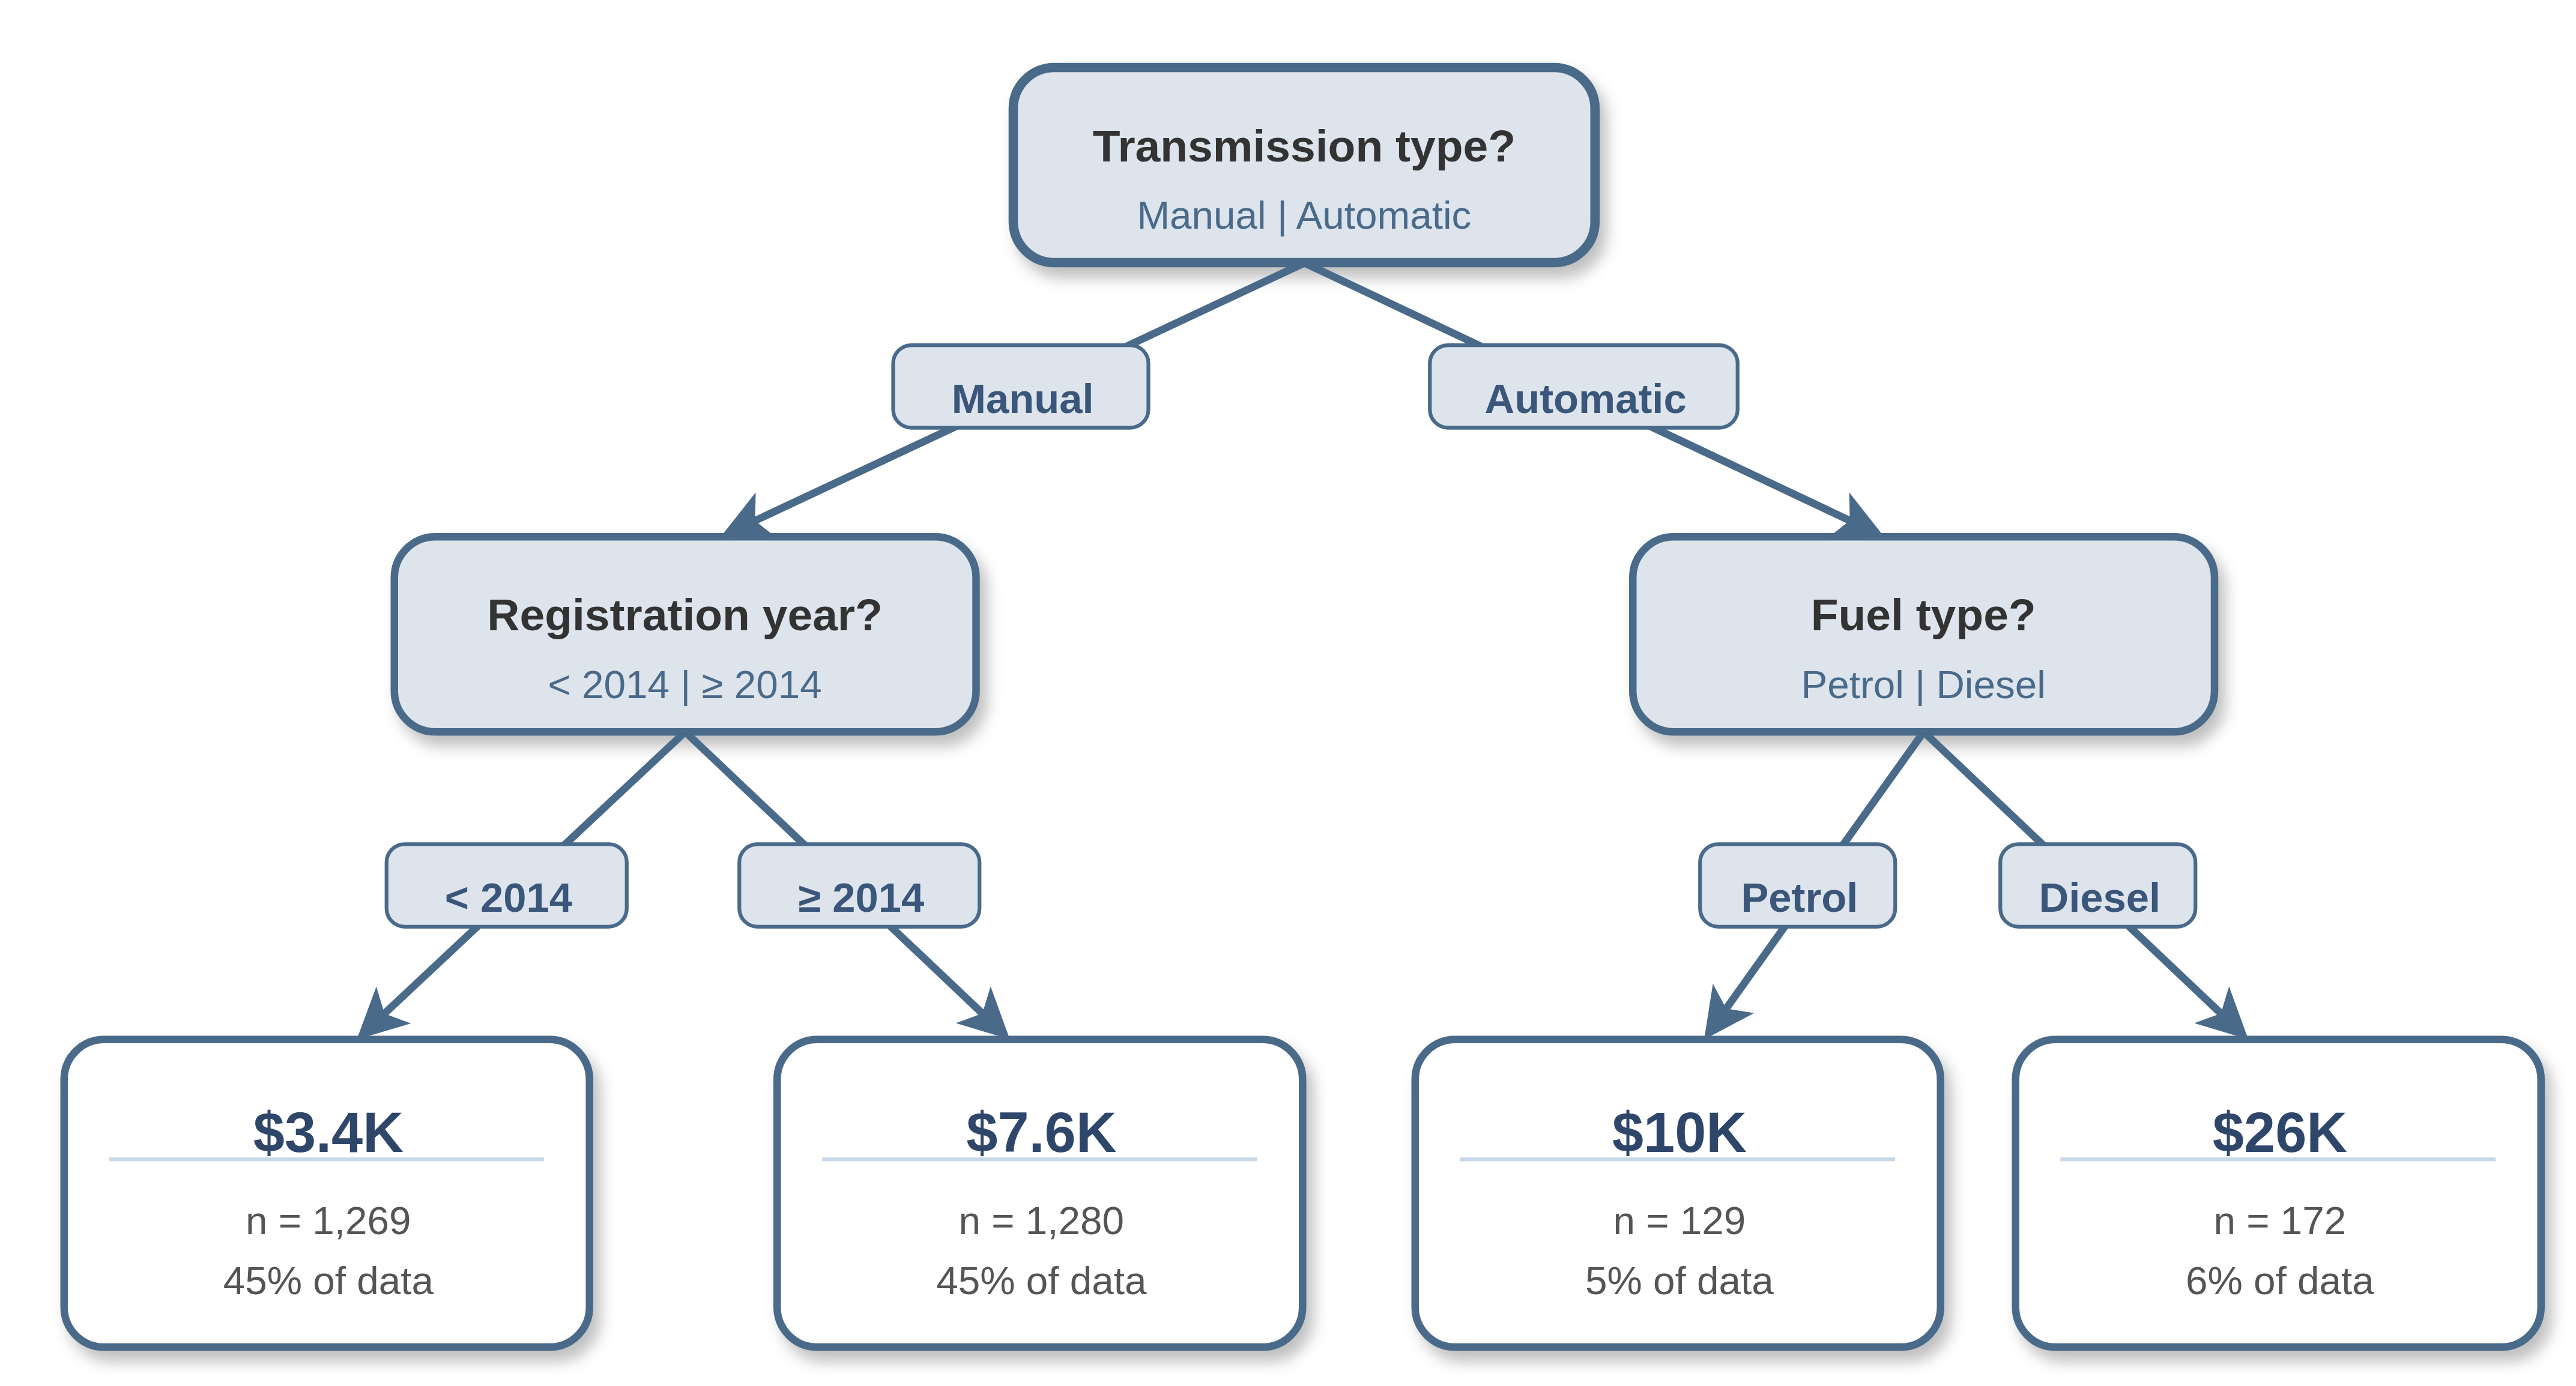
\includegraphics[width=0.7\linewidth,height=\textheight,keepaspectratio]{Figures/forests/fig-p3c14-cars-tree.png}

}

\caption{\label{fig-p3c14-cars-tree}Predicting the price a vehicle is
sold for in India using a regression tree, dataset from
kaggle.com/datasets/nehalbirla/vehicle-dataset-from-cardekho. Filled
rectangles with arrows (edges) coming off them are nodes, which indicate
the variable that is being split. Edges are branches, which indicate the
cutoff at which the variable is split. Variables are car transmission
type (manual or automatic), fuel type (petrol or diesel) and
registration year. The number at the top of the terminal nodes (unfilled
rectangles) is the average selling price for all observations in that
leaf. The numbers at the bottom of each leaf are the number of
observations in the leaf, and the proportion of data contained in the
leaf.}

\end{figure}%

\subsubsection{Splitting and stopping
rules}\label{splitting-and-stopping-rules}

Precisely how the data partitions/splits are derived and which variables
are utilized is determined by the \emph{splitting
rule}.\index{random forests!splitting rule} The goal in each partition
is to find two resulting nodes that have the greatest difference between
them and thus the maximal homogeneity within each node. Hence, after
each split, the data in each node should become increasingly similar.
The splitting rule provides a way to measure the difference between
nodes or the homogeneity within the resulting nodes. In regression, the
most common splitting rule is to select a variable and cutoff (a
threshold on the variable at which to separate observations) that
minimizes the mean squared error in the two potential resulting nodes.

For all decision tree and random forest algorithms going forward, let
\(\mathcal{A}\) denote the set of observation indices in a node, with
mean outcome:

\[
\bar{y}_{\mathcal{A}} = \frac{1}{\vert \mathcal{A} \vert}\sum_{i \in \mathcal{A}} y_i.
\]

Let \(j = 1,\ldots,p\) index the features and let \(c_j\) be a possible
cutoff value for feature \(j\). For parent node \(\mathcal{A}\), define:

\[
\begin{aligned}
&\mathcal{A}^l(j,c_j) := \{i \in \mathcal{A}: x_{i,j} < c_j\}, \\
&\mathcal{A}^r(j,c_j) := \{i \in \mathcal{A}: x_{i,j} \geq c_j\},
\end{aligned}
\]

as the two nodes resulting from partitioning feature \(j\) at cutoff
\(c_j\). To simplify notation, let \(\mathcal{A}^l, \mathcal{A}^r\)
denote \(\mathcal{A}^l(j,c_j)\) and \(\mathcal{A}^r(j,c_j)\)
respectively. The optimal split is determined by the arguments
\((j^*, c^*_{j^*})\) that minimize the residual sum of squares across
both nodes (James et al. 2013),

\[
(j^*, c_{j^*}^*) = \mathop{\mathrm{arg\,min}}_{j, c_j} \sum_{i \in \mathcal{A}^l} (y_i - \bar{y}_{\mathcal{A}^l})^2 + \sum_{i \in \mathcal{A}^r} (y_i - \bar{y}_{\mathcal{A}^r})^2.
\]

This method is repeated from the first node to the last such that
observations are included in a given node \(\mathcal{A}\) if they
satisfy all conditions from all previous branches (splits); features may
be considered multiple times in the growing process allowing complex
interaction effects to be captured.

Nodes are repeatedly split until a \emph{stopping rule} has been
triggered --- a criterion that tells the algorithm to stop partitioning
data.\index{random forests!stopping rule} The stopping rule is usually a
condition on the number of observations in each node such that nodes
will continue to be split until some minimum number of observations has
been reached in a node. Other conditions may be on the depth of the tree
(as in Figure~\ref{fig-p3c14-cars-tree} which is restricted to a maximum
depth of 2), which corresponds to the number of levels of
splitting.\index{random forests!hyperparameters!maximum depth} Stopping
rules are often used together, for example by setting a maximum tree
depth \emph{and} prespecifying a minimum number of observations per
leaf. Deciding the minimum number of observations and/or the maximum
depth can be performed with tuning (Section~\ref{sec-ml-opt}).

\subsubsection{Terminal node predictions}\label{sec-tree-terminal-nodes}

The final major component of decision trees is \emph{terminal node
predictions}.\index{random forests!terminal node} As the name suggests,
this is the part of the algorithm that determines how to actually make a
prediction for a new observation. A prediction is made by `dropping' the
new data `down' the tree according to the optimal splits that were found
during training. The resulting prediction is then a simple baseline
statistic computed from the training data in the corresponding node. In
regression, this is commonly the sample mean of the training outcome
data.

Returning to Figure~\ref{fig-p3c14-cars-tree}, say a new data point is
\{transmission = Manual, fuel = Diesel, year = 2015\}, then in the first
split the left branch is taken as `transmission = Manual', in the second
split the right branch is taken as `year' \(= 2015 \geq 2014\), hence
the new data point lands in the second terminal leaf and is predicted to
sell for \(7,600\). The `fuel' variable is ignored as it is only
considered for automatic vehicles.
Figure~\ref{fig-p3c14-cars-prediction-path} illustrates this prediction
path through the tree. This also highlights another powerful feature of
random forests: as the final predictions are simple statistics based on
training data, all potential predictions can be saved in the original
trained model and no complex computations are required in the prediction
algorithm.

\begin{figure}

\centering{

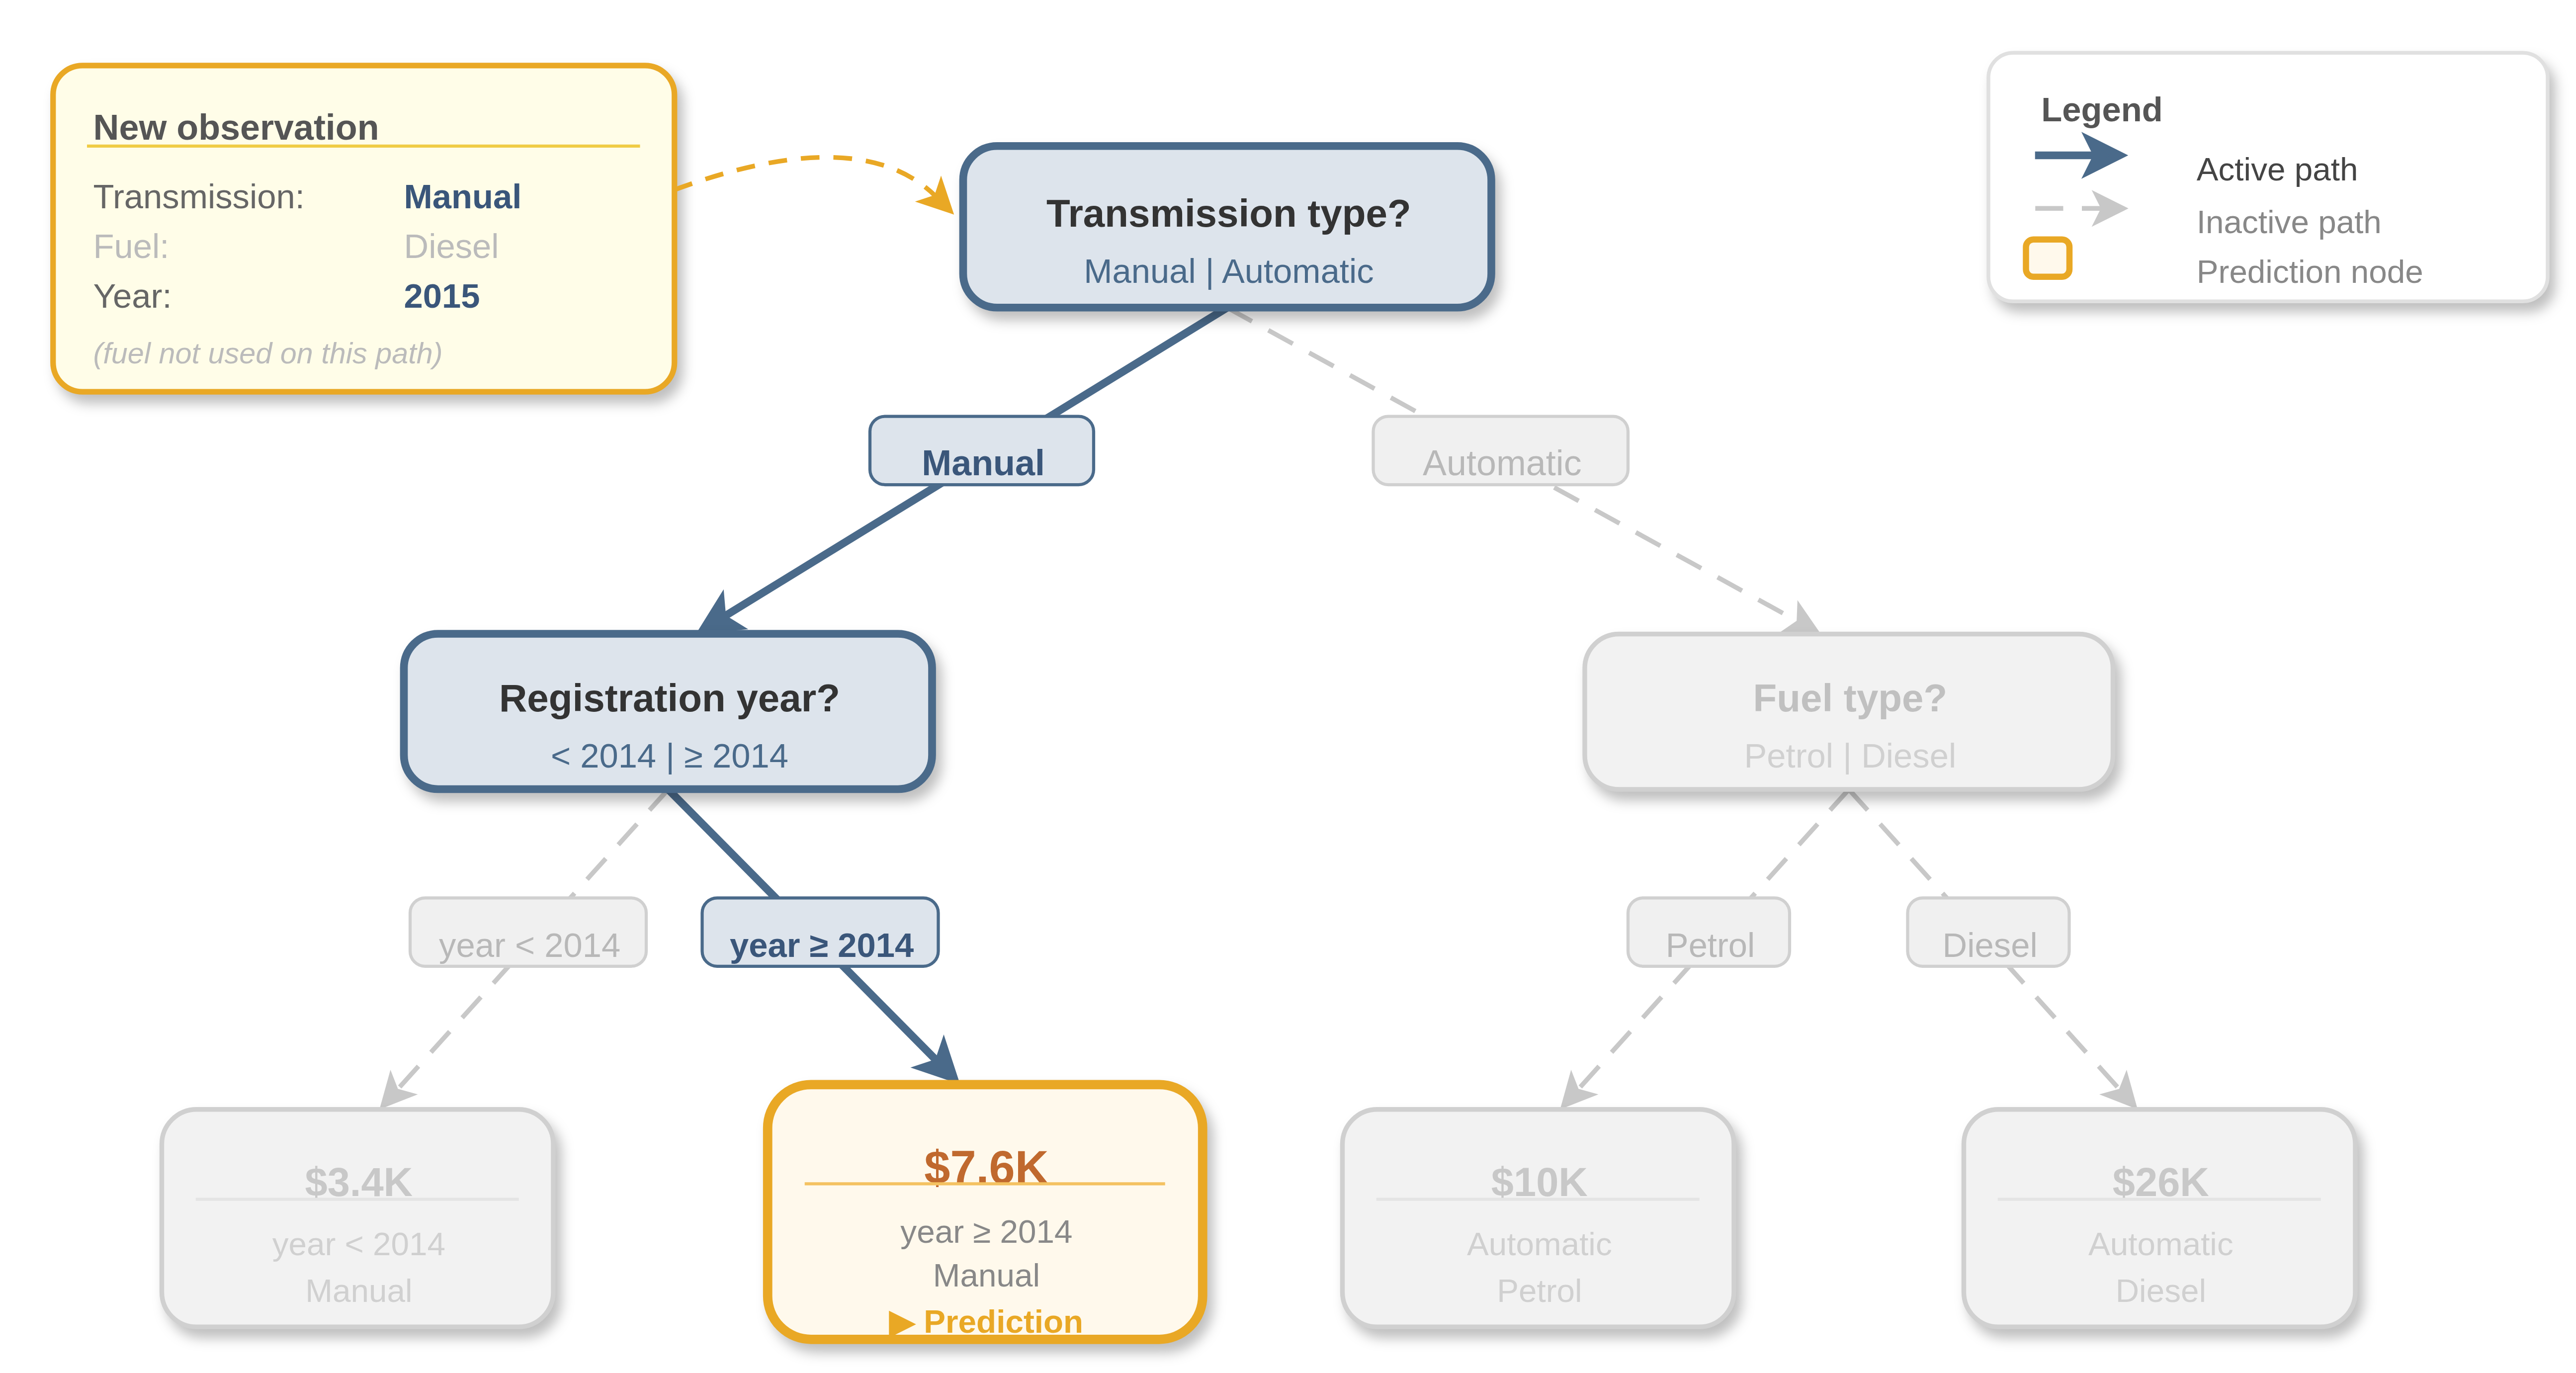
\includegraphics[width=0.7\linewidth,height=\textheight,keepaspectratio]{Figures/forests/fig-p3c14-cars-prediction-path.png}

}

\caption{\label{fig-p3c14-cars-prediction-path}Prediction path through
the regression tree from Figure~\ref{fig-p3c14-cars-tree} for a new
observation with transmission = Manual, fuel = Diesel, year = 2015. The
active path (solid blue arrows) leads through the `transmission =
Manual' split and the `year \(\geq\) 2014' split to the terminal node
predicting a sale price of \$7.6K (amber border). Inactive branches are
shown in gray with dashed lines. The `fuel' variable is not used on this
path, as fuel type is only evaluated for automatic vehicles.}

\end{figure}%

\subsection{Random forests}\label{random-forests}

Decision trees often overfit the training data, hence they have high
variance, perform poorly on new data, and are not robust to even small
changes in the original training data.\index{overfitting} Moreover,
important variables can end up being ignored as only subsets of dominant
variables are selected for splitting.

\emph{Random forests} treat individual decision trees as high-variance
base learners. Each tree may be unstable on its own, but averaging
predictions over many decorrelated trees produces a more stable
predictor.\index{random forests} Random forests utilize bootstrap
aggregation, or \emph{bagging} (Leo Breiman 1996), to aggregate many
decision trees as follows:\index{bagging}

\begin{enumerate}
\def\labelenumi{\arabic{enumi}.}
\tightlist
\item
  \textbf{for} \(b = 1,\ldots,B\):
\item
  ~~~~~\(D_b \gets \text{ Randomly sample with replacement from } \mathcal{D}_{train}\)
\item
  ~~~~~\(\hat{g}_b \gets \text{ Train a decision tree on } D_b\)
\item
  \textbf{end for}
\item
  \textbf{return} \(\{\hat{g}_b\}^B_{b=1}\)
\end{enumerate}

Step 2 is known as \emph{bootstrapping}, which is the process of
sampling a dataset \emph{with} replacement.\index{bootstrapping} In
random forest implementations this is more common than standard
subsampling where data is sampled \emph{without} replacement. Commonly,
the bootstrapped sample size is the same as the original. However, as
the same value may be sampled multiple times, on average the resulting
data only contains around 63.2\% unique observations (Efron and
Tibshirani 1997). Randomness is further injected to decorrelate the
trees by randomly subsetting the candidates of features to consider at
each split of a tree. Therefore, every split of every tree may consider
a different subset of variables.\index{random forests!decorrelation}
This process is repeated for \(B\) trees, with the final output being a
collection of trained decision trees. The number of trees is a
hyperparameter, but in
practice\index{random forests!hyperparameters!number of trees} \(B\) is
usually chosen to be large, with an early stopping-type procedure
(Section~\ref{sec-ml-early-stopping}) used to grow trees until
validation performance stabilizes.\index{early stopping} Beyond this
point, additional trees mainly increase computational cost while
providing diminishing improvements in predictive performance.

Prediction from a random forest for new data \(\mathbf{x}_*\) follows by
making predictions from the individual trees and aggregating the results
by some function \(\sigma\), which is usually the sample mean for
regression:

\[
\hat{g}(\mathbf{x}_*) = \sigma(\hat{g}_1(\mathbf{x}_*),\ldots,\hat{g}_B(\mathbf{x}_*)) = \frac{1}{B} \sum^B_{b=1} \hat{g}_b(\mathbf{x}_*)
\]

where \(\hat{g}_b(\mathbf{x}_*)\) is the prediction from the \(b\)th
tree for some new data \(\mathbf{x}_*\) and \(B\) is the total number of
grown trees.

As discussed above, individual decision trees result in predictions with
high variance that are not robust to small changes in the underlying
data. Random forests decrease this variance by aggregating predictions
over a large sample of decorrelated trees, where a high degree of
difference between trees is promoted through the use of bootstrapped
samples and random candidate feature selection at each split.

Usually many (hundreds or thousands) trees are grown, which makes random
forests robust to changes in data with more stable predictions. Other
advantages include having tunable and meaningful hyperparameters,
including: the number of variables to consider for a single split, the
splitting rule, and the stopping rule.

While random forests are considered a black box, in that one cannot be
reasonably expected to inspect thousands of individual trees, variable
importance\index{variable importance} can still be aggregated across
trees, for example by counting the frequency a variable was selected
across trees, calculating the minimal depth at which a variable was used
for splitting, or via permutation-based feature importance. Hence random
forest models are usually more interpretable than many alternative
methods. Finally, random forests are less prone to overfitting than
individual trees as predictions are averaged across many decorrelated
trees.

\section{Random survival forests}\label{random-survival-forests}

Random forests can be adapted to \emph{random survival forests} by
updating the splitting rules and terminal node predictions to those that
can handle censoring and can make survival
predictions.\index{random survival forests} This chapter is therefore
focused on outlining different choices of splitting rules and terminal
node predictions, which can then be flexibly combined into different
models.

\subsection{Splitting rules}\label{splitting-rules}

Survival trees and random survival forests (RSFs) have been studied for
the past four decades and while there are many possible splitting rules
(Bou-Hamad, Larocque, and Ben-Ameur 2011), only two broad classes are
commonly utilized (as judged by number of available implementations, for
example, Ishwaran et al. 2011; Pölsterl 2020; Wright and Ziegler 2017).
\index{random survival forests!splitting rules} The first class relies
on the log-rank
test\index{random survival forests!splitting rules!log-rank test} to
maximize dissimilarity between splits, the second class utilizes
likelihood-based measures. The first is discussed in more detail as this
is common in practice and is relatively straightforward to implement and
understand. Likelihood rules are more complex and may require
assumptions that are not realistic, these are discussed briefly.

\subsubsection{Log-rank test}\label{log-rank-test}

The log-rank test statistic has been widely utilized as a splitting rule
for survival analysis (Ciampi et al. 1986; Ishwaran et al. 2008; LeBlanc
and Crowley 1993; Segal
1988).\index{random survival forests!splitting rules!log-rank test} The
log-rank test compares the survival distributions of two groups under
the null hypothesis that both groups have the same underlying risk of
(immediate) events, with the hazard function used to compare underlying
risk.

Let \(\mathcal{A}^l\) and \(\mathcal{A}^r\) be two nodes, and as before
\(i \in \mathcal{A}\) indexes the observations in node \(\mathcal{A}\).
Define:

\begin{itemize}
\item
  \(n_\tau^l\), the number of observations at risk at time point
  \(\tau\) in node \(\mathcal{A}^l\) \[
  n_\tau^l = \sum_{i \in \mathcal{A}^l} \mathbb{I}(t_i \geq \tau);
  \]
\item
  \(o^l_{\tau}\), the observed number of events at time point \(\tau\)
  in node \(\mathcal{A}^l\)
\end{itemize}

\[
o^l_{\tau} = \sum_{i \in \mathcal{A}^l} \mathbb{I}(t_i = \tau, \delta_i = 1);
\]

\begin{itemize}
\tightlist
\item
  \(n_\tau = n_\tau^l + n_\tau^r\), the number of observations at risk
  at \(\tau\) in both nodes;
\item
  \(o_\tau = o^l_{\tau} + o^r_{\tau}\), the observed number of events at
  \(\tau\) in both nodes.
\end{itemize}

Recall \(t_{(k)}\) is the \(k\)th ordered event time. The log-rank test
evaluates if hazard functions are equal in both nodes,
\(H_0: h^l = h^r\), with test statistic (Segal 1988),

\[
LR(\mathcal{A}^l) = \frac{\sum_{k=1}^m (o^l_{t_{(k)}} - e^l_{t_{(k)}})}{\sqrt{\sum_{k=1}^m v_{t_{(k)}}^l}},
\]

where:

\begin{itemize}
\tightlist
\item
  \(e^l_{\tau}\) is the expected number of events in node
  \(\mathcal{A}^l\) at \(\tau\):
\end{itemize}

\[
e^l_{\tau} := o_\tau\frac{n_\tau^l}{n_\tau};
\]

\begin{itemize}
\tightlist
\item
  \(v^l_\tau\) is the variance of the number of events in node
  \(\mathcal{A}^l\) at \(\tau\):
\end{itemize}

\[
v^l_{\tau} := e^l_{\tau} \Big(\frac{n_\tau - o_\tau}{n_\tau}\Big)\Big(\frac{n_\tau - n^l_\tau}{n_\tau - 1}\Big).
\]

These results follow from the assumption that, under equal hazards in
both nodes, the number of events at each unique event time follows a
hypergeometric distribution. \index{hypergeometric distribution} Under
\(H_0\), \(LR(\mathcal{A}^l)^2\) follows a \(\chi^2\) distribution with
one degree of freedom and the log-rank statistic is commonly reported
alongside its corresponding \(p\)-value. In the two group setting,
\(LR(\mathcal{A}^l) = -LR(\mathcal{A}^r)\), hence it is sufficient to
compute the statistic for only one of the two nodes.

The higher the (absolute) log-rank statistic, the greater the
dissimilarity between the two groups (Figure~\ref{fig-p3c14-logrank}),
thereby making it a sensible splitting rule for random forests; it has
also been shown that it works well for splitting censored data (LeBlanc
and Crowley 1993). Additionally, the log-rank test requires no knowledge
about the shape of the survival curves or distribution of the outcomes
in either group (Bland and Altman 2004), making it ideal for an
automated process that requires no user intervention.

\begin{figure}

\centering{

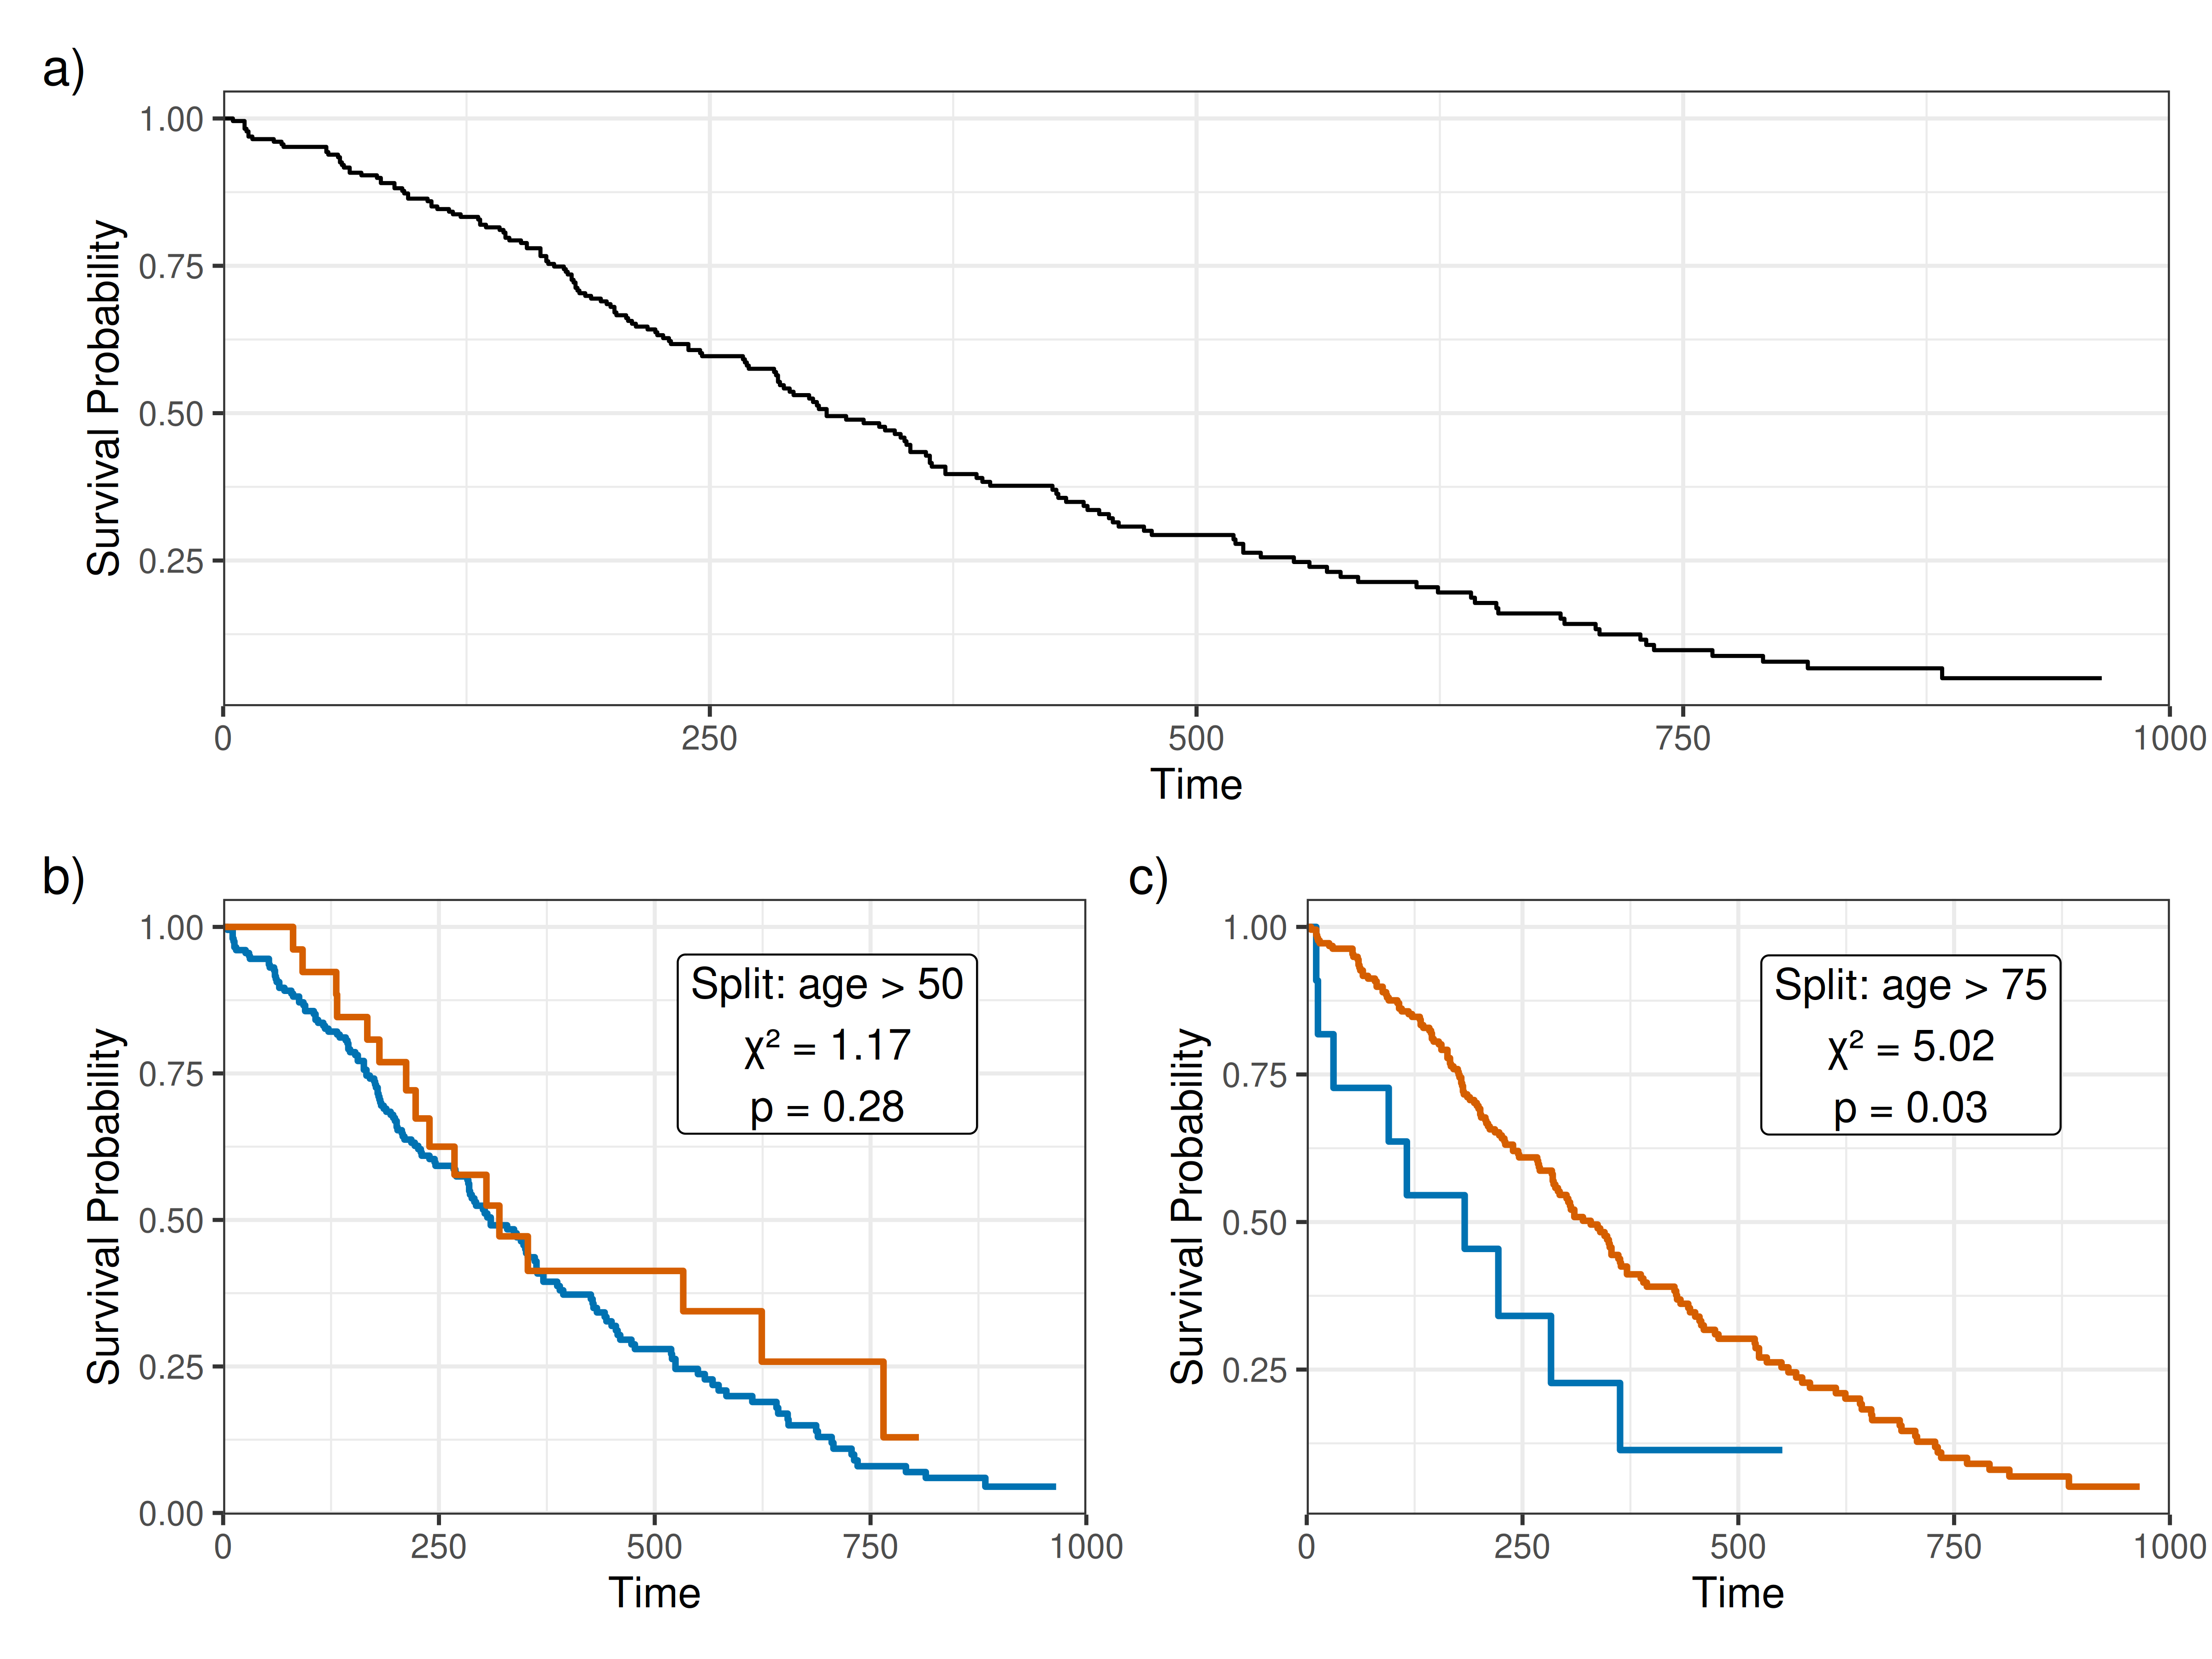
\includegraphics[width=0.9\linewidth,height=\textheight,keepaspectratio]{Figures/forests/fig-p3c14-logrank.png}

}

\caption{\label{fig-p3c14-logrank}Panel (a) is the Kaplan-Meier
estimator fit on the complete \texttt{lung} dataset from the
\(\textsf{R}\) package \texttt{survival}. (b-c) is the same data
stratified according to whether `age' is greater or less than 50 (panel
b) or 75 (panel c). The higher \(\chi^2\) statistic (panel c) results in
a lower \(p\)-value and a greater difference between the stratified
Kaplan-Meier curves. Therefore, splitting age at 75 results in a greater
dissimilarity between the resulting branches and thus makes a better
choice for splitting the variable.}

\end{figure}%

The log-rank \emph{score} rule (Hothorn and Lausen 2003) is a
standardized version of the log-rank rule that could be considered as a
splitting rule, though simulation studies have not demonstrated
significant improvements in predictive performance when comparing the
two (Ishwaran et al.
2008).\index{random survival forests!splitting rules!log-rank score}
Alternative dissimilarity measures and tests have also been suggested as
splitting rules, including modified Kolmogorov-Smirnov test and
Gehan-Wilcoxon tests (Ciampi et al.
1988).\index{random survival forests!splitting rules!Kolmogorov-Smirnov}\index{random survival forests!splitting rules!Gehan-Wilcoxon}
Simulation studies have demonstrated that both of these may have higher
power and produce `better' results than the log-rank statistic (Fleming
et al. 1980), however neither appears to be commonly used.

\subsubsection{Alternative splitting
rules}\label{alternative-splitting-rules}

A splitting rule is simply a way to measure if average performance
across resulting nodes increases after data splitting. Therefore, there
are many statistics that could be used for this purpose (Gordon and
Olshen 1985; Ishwaran and Kogalur 2018; Schmid, Wright, and Ziegler
2016), including many of the metrics referenced in Part II. Like many
other aspects of modeling, experiments have shown that the choice of
splitting rules is data dependent (Schmid, Wright, and Ziegler 2016).
When using loss-based splitting rules, a sensible approach is to align
the splitting rule with the prediction problem. The log-rank splitting
rule is commonly used when the goal is to maximize homogeneity within
each node; for example, to most accurately estimate the within-node
survival distribution. However, if the goal were to optimize the ranking
of observations, then a concordance splitting rule may be optimal
(Section~\ref{sec-cindex}).

An alternative to log-rank statistics and loss-based splitting rules is
to instead use \emph{likelihood ratio}, or \emph{deviance}, statistics
(LeBlanc and Crowley 1992). The likelihood-ratio statistic evaluates
whether model fit improves after a candidate split and can therefore be
used as a natural splitting
rule.\index{random survival forests!splitting rules!likelihood ratio} An
advantage of likelihood-based methods is that alternative censoring
mechanisms and truncation can be incorporated naturally through the
likelihood formulation (\ref{eq-objective-function}). However,
specifying an appropriate parametric form for each fit is non-trivial,
and assumptions that poorly reflect the data may lead to inferior
splits. In principle, likelihood-based splitting rules may yield trees
that better fit the data. Random forests are built from many base
learners whose predictions are stabilized through averaging, so
optimizing the fit of each individual tree may be unnecessary and any
gains may be outweighed by sensitivity to model assumptions. Moreover,
likelihood-based methods are implemented in relatively few off-the-shelf
software packages and there is limited research formally comparing them
with alternative splitting rules.

\subsection{Terminal node
prediction}\label{sec-surv-ml-models-ranfor-nodes}

Similarly to the regression setting, RSF predictions are typically based
on simple estimates computed from the training data that fall within the
terminal nodes. As seen throughout this book, the choice of estimator in
the survival setting depends on the prediction task of
interest.\index{random survival forests!terminal node prediction} This
section focuses on probabilistic predictions for the single-event
setting, extensions to competing risks are discussed in
Section~\ref{sec-surv-ranfor-cr}, and then relative risk predictions for
both settings are described in Section~\ref{sec-rsf-risks}.

Terminal node predictions are only useful when there are sufficient
uncensored observations in each terminal node. Hence, a common RSF
stopping rule is to set a threshold on the minimum number of
\emph{uncensored} observations per node, meaning that a node is not
split if doing so would result in too few uncensored observations to
make meaningful
predictions.\index{random survival forests!stopping rule}\index{random survival forests!hyperparameters!minimum node size}
When the minimum uncensored node size is not exposed as a
hyperparameter, it can be tuned indirectly through the standard minimum
node size. Alternatively, a useful heuristic is to take the recommended
default minimum node size and divide it by the uncensored proportion in
the data. For example, if the default minimum node size is \(10\) and
\(30\%\) of the data are censored, then the adjusted minimum node size
is \(\lceil 10/0.7 \rceil = 15\).

For survival distribution predictions, the algorithm requires a simple
estimate for the underlying survival distribution in each of the
terminal nodes, which can be estimated using the Kaplan-Meier
(\ref{eq-km}) or Nelson-Aalen (\ref{eq-nelson-aalen}) estimators
(Hothorn et al. 2004; Ishwaran et al. 2008; LeBlanc and Crowley 1993;
Segal 1988).\index{Kaplan-Meier estimator}\index{Nelson-Aalen estimator}

Let \(b \in \{1,\ldots,B\}\) index the trees in a forest, let
\(\mathcal{A}_b(\mathbf{x}_*)\) denote the terminal node in tree \(b\)
that observation \(\mathbf{x}_*\) falls into, and let
\(t^*_{(1)} < \ldots < t^*_{(m)}\) be the ordered event times within
\(\mathcal{A}_b(\mathbf{x}_*)\). Then the predicted survival function
and cumulative hazard for \(\mathbf{x}_*\) are,

\begin{equation}\phantomsection\label{eq-rsf-surv-kaplan}{
\hat{S}_{b}(\tau \mid \mathbf{x}_*) = \prod_{k:t^*_{(k)} \leq \tau} \left(1-\frac{d_{t^*_{(k)}}}{n_{t^*_{(k)}}}\right),
}\end{equation}

and,

\begin{equation}\phantomsection\label{eq-rsf-surv-nelson}{
\hat{H}_{b}(\tau \mid \mathbf{x}_*) = \sum_{k:t^*_{(k)} \leq \tau} \frac{d_{t^*_{(k)}}}{n_{t^*_{(k)}}},
}\end{equation}

where \(d_{t^*_{(k)}}\) and \(n_{t^*_{(k)}}\) are the observed number of
events and the number of observations at risk at \(t^*_{(k)}\), both
computed from observations in \(\mathcal{A}_b(\mathbf{x}_*)\). Direct
calculation of the cumulative hazard using (\ref{eq-rsf-surv-nelson})
avoids \(\log(0)\) errors which could occur if transforming from the
Kaplan-Meier estimates in (\ref{eq-rsf-surv-kaplan}). See
Figure~\ref{fig-p3c14-lung-tree} for an example using the \texttt{lung}
dataset (Therneau 2024).

\begin{figure}

\centering{

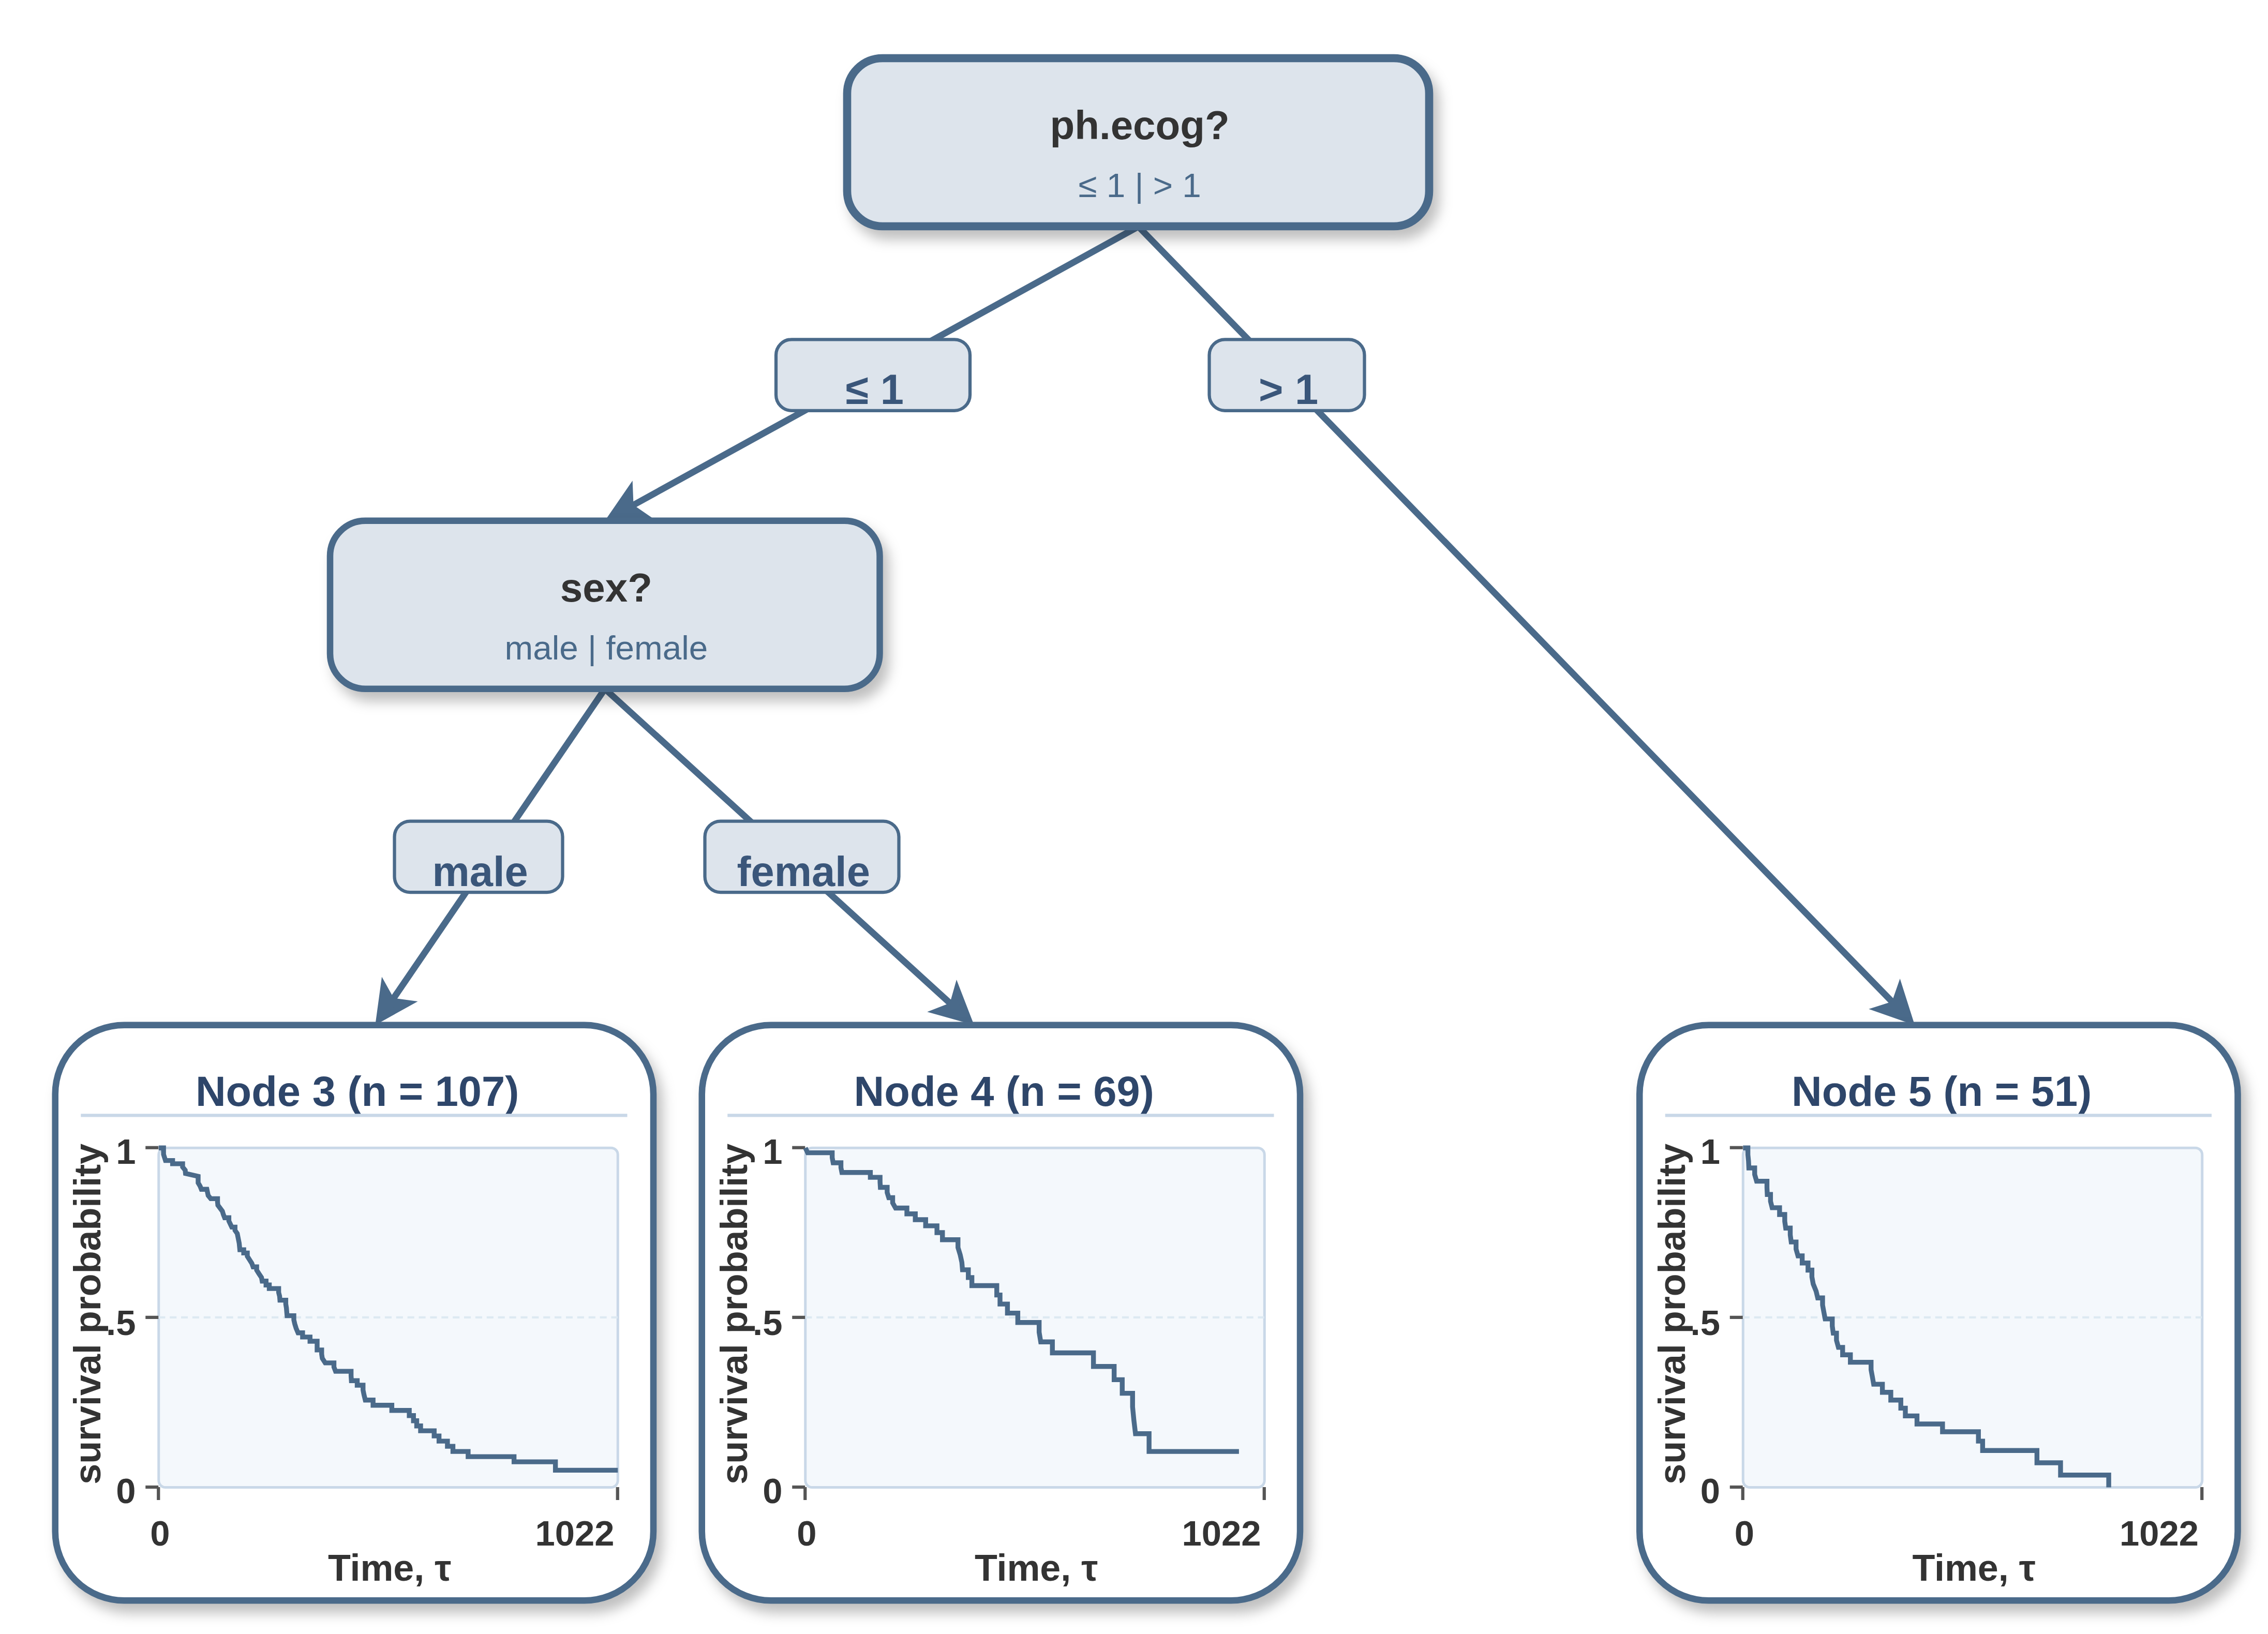
\includegraphics[width=0.7\linewidth,height=\textheight,keepaspectratio]{Figures/forests/fig-p3c14-lung-tree.png}

}

\caption{\label{fig-p3c14-lung-tree}Survival tree trained on the
\texttt{lung} dataset from the \(\textsf{R}\) package \texttt{survival}.
The terminal node predictions are survival curves.}

\end{figure}%

The bootstrapped prediction may be formed either by averaging survival
or cumulative hazard functions over individual
trees.\index{random survival forests!bagging} By definition, a mixture
of \(n\) distributions with cumulative distribution functions
\(F_i, i = 1,\ldots,n\) is given
by,\index{random survival forests!terminal node prediction}

\[
F(x) = \sum^n_{i=1} w_i F_i(x),
\]

for some weights \(w_i, i = 1, \ldots, n\). Substituting \(F = 1 - S\)
and noting \(\sum w_i = 1\) gives the computation
\(S(x) = \sum^n_{i=1} w_i S_i(x)\), allowing the bootstrapped survival
function to exactly represent the mixture distribution defined by the
tree-specific survival functions:

\begin{equation}\phantomsection\label{eq-surv-kaplan-boot}{
\hat{S}_{Boot}(\tau \mid \mathbf{x}_*) = \sum^B_{b=1} w_b\hat{S}_b(\tau \mid \mathbf{x}_*),
}\end{equation}

usually with \(w_b = 1/B\) where \(B\) is the number of trees.
Alternatively, an ensemble estimator can be taken over the cumulative
hazards:

\begin{equation}\phantomsection\label{eq-surv-nelson-boot}{
\hat{H}_{Boot}(\tau \mid \mathbf{x}_*) = \sum^B_{b=1} w_b\hat{H}_b(\tau \mid \mathbf{x}_*).
}\end{equation}

The cumulative hazard ensemble (\ref{eq-surv-nelson-boot}) does not
generally correspond to the cumulative hazard of a mixture distribution,
since
\(\hat{S}_{Boot}(\tau \mid \mathbf{x}_*) \ne \exp(-\hat{H}_{Boot}(\tau \mid \mathbf{x}_*))\),
though this does not affect its validity as an ensemble estimator.

In other censoring and truncation settings, the estimator in the final
node can be replaced by the non-parametric maximum likelihood estimator
or left-truncated risk set
(Section~\ref{sec-surv-estimation-non-param}).

An important practical consideration is how to average survival
probabilities across decision trees, as each individual non-parametric
estimate may be defined on different event times. This is addressed by
leveraging the fact that non-parametric estimators are step functions.
For example, the Kaplan-Meier estimator is constant between event times
and equal to the most recently observed survival probability,
effectively allowing the estimator to make predictions at arbitrary time
points as discussed in (Section~\ref{sec-classical-nonpar}).
Figure~\ref{fig-p3c14-bootstrap} demonstrates the process for three
decision trees, where panel (a) shows the estimates within three
terminal nodes (red, green, blue). Each Kaplan-Meier estimator is
evaluated at the union of observed event times across trees (panels
b-c), and the resulting survival probabilities are averaged at each time
point to obtain the bootstrapped survival estimate
(\ref{eq-surv-kaplan-boot}), shown in panel (d).

\begin{figure}

\centering{

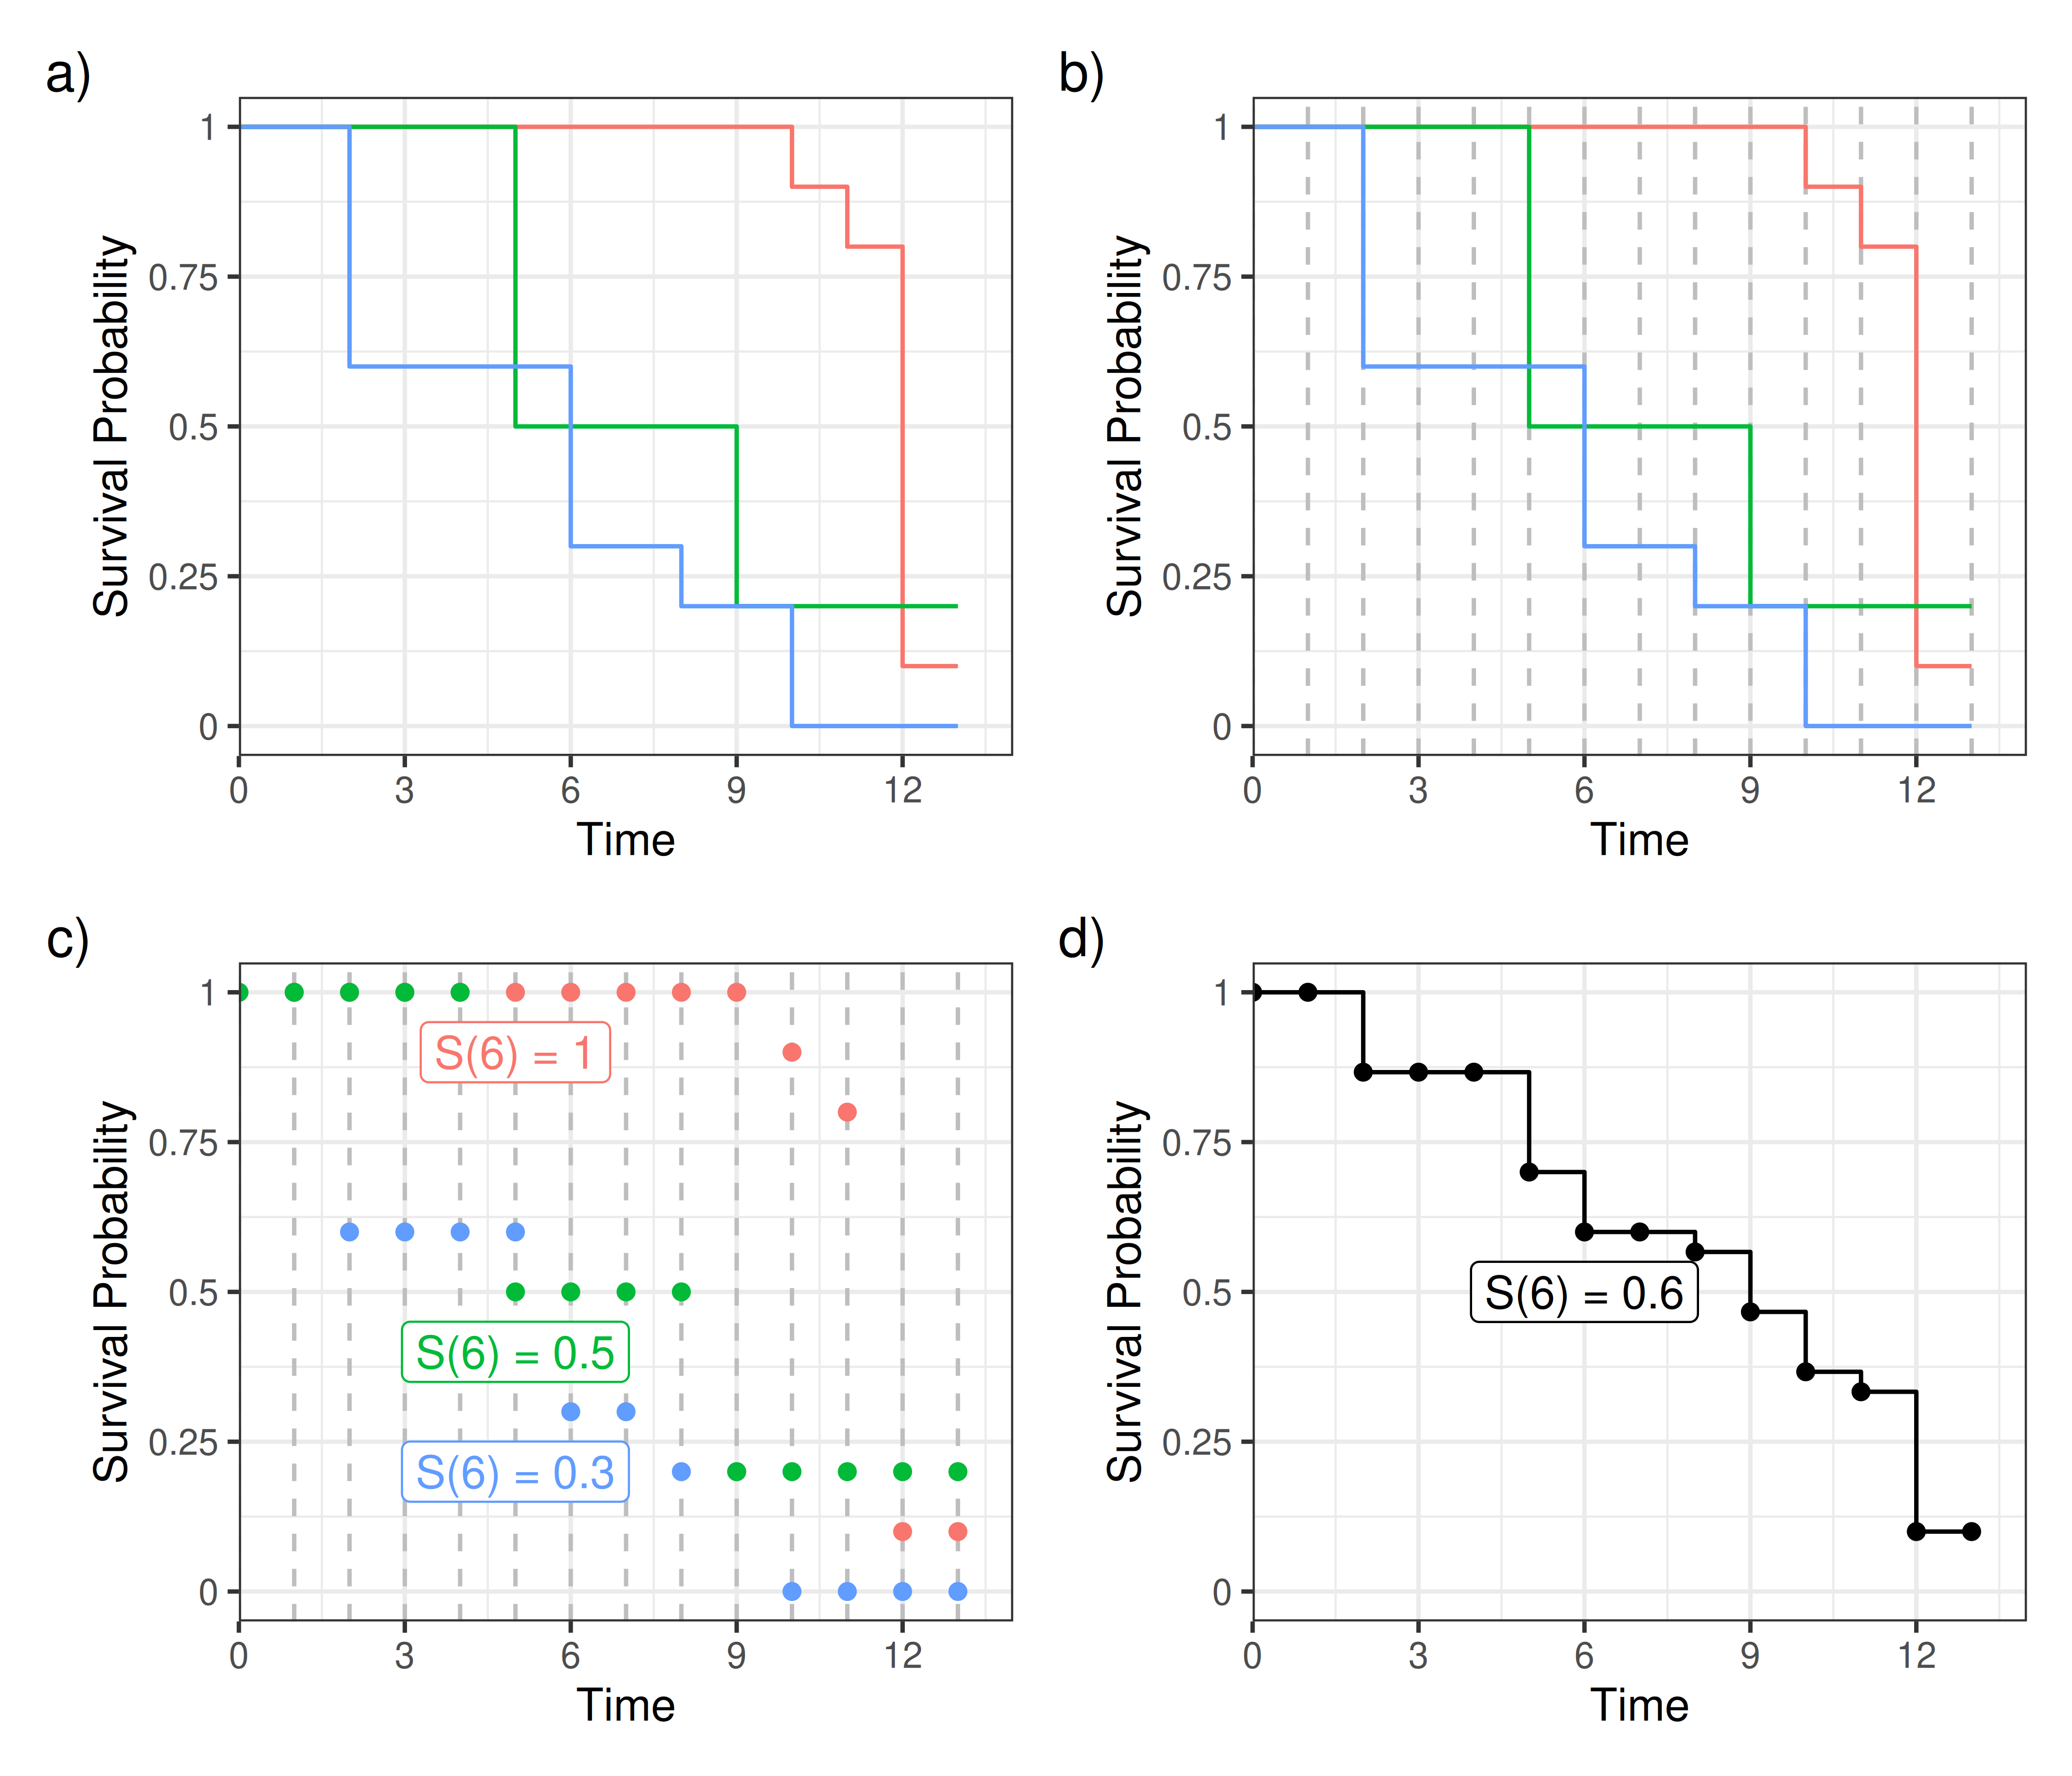
\includegraphics[width=0.9\linewidth,height=\textheight,keepaspectratio]{Figures/forests/fig-p3c14-bootstrap.png}

}

\caption{\label{fig-p3c14-bootstrap}Bootstrapping Kaplan-Meier
estimators across three decision trees (red, blue, green). Panel a)
shows the individual estimates, b) shows the time points to aggregate
the trees over, c) is the predicted survival probability from each tree
at all event times, and d) is the average survival probabilities
connected by a step function.}

\end{figure}%

\subsection{Competing risks}\label{sec-surv-ranfor-cr}

The RSF framework extends to competing risks
(Section~\ref{sec-competing-risks}) in a natural way, replacing the
single-event Kaplan-Meier and Nelson-Aalen estimators in the terminal
nodes with the Aalen-Johansen CIF estimator
(Section~\ref{sec-aalen-johansen}; Ishwaran et al. (2014)).
\index{random survival forests!competing risks} Both the splitting rule
and the terminal node estimator must be adapted to account for the
presence of multiple event types.

\subsubsection{Splitting rules}\label{splitting-rules-1}

Splitting rules can be separated into \emph{cause-specific} and
\emph{composite} splitting rules (Ishwaran et al. 2014). Cause-specific
rules target a single cause \(q\) and are appropriate when the primary
interest is in one particular cause. Composite rules aggregate
information across all \(Q\) causes and are appropriate when the goal is
to predict all cause-specific hazards or CIFs simultaneously. Composite
rules produce a single splitting statistic by taking a variance-weighted
sum of the per-cause statistics across all \(Q\) causes (Ishwaran et al.
2014).
\index{random survival forests!competing risks!composite splitting rules}

Two common splitting rules are the generalized log-rank rule and Gray's
test.\index{random survival forests!competing risks!cause-specific splitting rules}\index{random survival forests!competing risks!generalized log-rank test}\index{random survival forests!competing risks!Gray's test}
The \emph{generalized log-rank} rule tests \(H_0: h_q^l = h_q^r\), where
\(h_q\) is the hazard for cause \(q\), whereas \emph{Gray's test} tests
\(H_0: F_q^l = F_q^r\), where \(F_q\) is the CIF for cause \(q\).

\textbf{Generalized log-rank.}
\index{random survival forests!competing risks!generalized log-rank test}
The cause-\(q\) log-rank statistic treats competing events as censored,
so that the risk set for cause \(q\) consists of all subjects still at
risk for any event, with the number of subjects at risk denoted by
\(n_{\tau}\). The observed cause-\(q\) events in \(\mathcal{A}^l\) at
some \(\tau\) are:

\[
o^l_{q,{\tau}} = \sum_{i \in \mathcal{A}^l} \mathbb{I}(t_i = \tau,\, q_i = q),
\]

where \(q_i\) is the observed cause for observation \(i\). The expected
number of events under the null of equal cause-\(q\) hazards in both
nodes is:

\begin{equation}\phantomsection\label{eq-cr-exp}{
e^l_{q,{\tau}} = o_{q,{\tau}}\frac{n^l_{\tau}}{n_{\tau}},
}\end{equation}

where \(o_{q,{\tau}}\) and \(n_{\tau}\) are the corresponding totals
over both nodes. The per-cause statistic for \(m\) ordered event times,
\(t_{(k)}\), is:

\begin{equation}\phantomsection\label{eq-lr-cause-q}{
LR_q(\mathcal{A}^l) = \frac{\sum^m_{k=1} w_q({t_{(k)}})\,(o^l_{q,{t_{(k)}}} - e^l_{q,{t_{(k)}}})}{\sqrt{\sum^m_{k=1} w_q({t_{(k)}})^2\, v^l_{q,{t_{(k)}}}}},
}\end{equation}

where \(v^l_{q,{t_{(k)}}}\) is the hypergeometric variance for cause
\(q\) at \(t_{(k)}\), and \(w_q(t_{(k)}) > 0\) are time-dependent
weights that can be used to up-weight differences at the beginning or
end of follow-up (Harrington and Fleming 1982).

The composite log-rank statistic aggregates the per-cause statistics
(\ref{eq-lr-cause-q}) across all \(Q\) causes:

\[
LR_{CR}(\mathcal{A}^l) = \frac{\sum_{q=1}^Q \hat{\sigma}_q^2 \, LR_q(\mathcal{A}^l)}{\sqrt{\sum_{q=1}^Q \hat{\sigma}_q^2}}, \qquad \hat{\sigma}_q^2 = \sum_k w_q({t_{(k)}})^2\, v^l_{q,{t_{(k)}}};
\]

\textbf{Gray's test.}
\index{random survival forests!competing risks!Gray's test} While the
generalized log-rank rule detects variables that affect the cause-\(q\)
hazard, Gray's test (Gray 1988) instead tests \(H_0: F_q^l = F_q^r\),
thereby selecting variables according to differences in the cumulative
incidence of cause \(q\). As Gray's test targets the CIF directly, it
could be preferred when the CIF is the prediction of interest in the
competing risks setting (Ishwaran et al. 2014).

Following Ishwaran et al. (2014), the splitting statistic is obtained by
substituting an augmented risk set into (\ref{eq-cr-exp}) in place of
\(n_{t_{(k)}}\). Motivated by the Fine-Gray subdistribution hazard
framework (Section~\ref{sec-classical-ph-cr}), the augmented risk set
retains subjects who experienced a competing event before \(t_{(k)}\).
In practice, this is implemented by adding subjects who experienced a
competing event before \(t_{(k)}\) back into the risk set (Fine and Gray
1999):

\[
\tilde{n}_{q,t_{(k)}} = n_{t_{(k)}} + \sum_{j:\, t_{(j)} < t_{(k)}} \sum_{q' \neq q} d_{q',t_{(j)}}.
\]

The observed cause-\(q\) events are unchanged:

\[
o^l_{q,t_{(k)}} = \sum_{i \in \mathcal{A}^l} \mathbb{I}(t_i = t_{(k)},\, q_i = q).
\]

The expected count replaces \(n_{t_{(k)}}\) with
\(\tilde{n}_{q,t_{(k)}}\) (and \(n^l_{t_{(k)}}\) with
\(\tilde{n}^l_{q,t_{(k)}}\)) in (\ref{eq-cr-exp}):

\[
\tilde{e}^l_{q,t_{(k)}} = o_{q,t_{(k)}}\frac{\tilde{n}^l_{q,t_{(k)}}}{\tilde{n}_{q,t_{(k)}}}.
\]

The per-cause Gray statistic is then:

\[
\widetilde{LR}_q(\mathcal{A}^l) = \frac{\sum_{k} w_q(t_{(k)})\,(o^l_{q,t_{(k)}} - \tilde{e}^l_{q,t_{(k)}})}{\sqrt{\sum_{k} w_q(t_{(k)})^2\,\tilde{v}^l_{q,t_{(k)}}}},
\]

where \(\tilde{v}^l_{q,t_{(k)}}\) is the hypergeometric variance
(\ref{eq-lr-cause-q}) with \(\tilde{n}_{q,t_{(k)}}\) in place of
\(n_{t_{(k)}}\).

Similarly to the cause-specific case, the composite Gray statistic is:

\[
\widetilde{LR}(\mathcal{A}^l) = \frac{\sum_{q=1}^Q \tilde{\sigma}_q^2 \, \widetilde{LR}_q(\mathcal{A}^l)}{\sqrt{\sum_{q=1}^Q \tilde{\sigma}_q^2}}, \qquad \tilde{\sigma}_q^2 = \sum_k w_q(t_{(k)})^2\,\tilde{v}^l_{q,t_{(k)}}.
\]

\subsubsection{Terminal node prediction}\label{terminal-node-prediction}

Within each terminal node \(\mathcal{A}_b(\mathbf{x}_*)\), the
Aalen-Johansen estimator is used to estimate the CIF for each cause
\(q \in \{1, \ldots, Q\}\).

Let \(t^*_{(1)} < \ldots < t^*_{(m)}\) be the ordered event times (of
any cause) within \(\mathcal{A}_b(\mathbf{x}_*)\), and let
\(d_{q,t^*_{(k)}}\) and \(n_{t^*_{(k)}}\) denote the number of
cause-\(q\) events and the number at risk at \(t^*_{(k)}\), both
computed from observations in \(\mathcal{A}_b(\mathbf{x}_*)\). The
cause-specific discrete hazard (Section~\ref{sec-aalen-johansen}) within
the node is
\(\hat{h}^d_{q,b}(t^*_{(k)}) = d_{q,t^*_{(k)}} / n_{t^*_{(k)}}\), the
all-cause survival in the node is then,

\[
\hat{S}_b(\tau \mid \mathbf{x}_*) = \prod_{k: t^*_{(k)} \leq \tau} \left(1 - \sum_{q=1}^Q \hat{h}^d_{q,b}(t^*_{(k)})\right),
\]

and the CIF for cause \(q\) is the discrete Aalen-Johansen estimator,

\[
\hat{F}_{q,b}(\tau \mid \mathbf{x}_*) = \sum_{k: t^*_{(k)} \leq \tau} \hat{S}_b(t^*_{(k-1)} \mid \mathbf{x}_*) \hat{h}^d_{q,b}(t^*_{(k)}),
\]

with \(t^*_{(0)} = 0\).

Finally, the bootstrapped CIF prediction is the weighted average of the
per-tree Aalen-Johansen
estimates:\index{random survival forests!competing risks!bootstrapped CIF}

\[
\hat{F}_{q,Boot}(\tau \mid \mathbf{x}_*) = \sum_{b=1}^B w_b\hat{F}_{q,b}(\tau \mid \mathbf{x}_*).
\]

As with the bootstrapped Kaplan-Meier prediction
(\ref{eq-surv-kaplan-boot}), the ensemble CIF also represents a mixture
of the per-tree distributions.

\subsection{Relative risk predictions}\label{sec-rsf-risks}

The most common method to estimate the average relative risk appears to
be a transformation from the Nelson-Aalen method (Ishwaran et al. 2008),
which exploits results from counting processes to provide a measure of
expected mortality (Hosmer Jr, Lemeshow, and May 2011); the same result
is used in the event frequency calibration measure discussed in
Section~\ref{sec-alpha}.
\index{random survival forests!relative risk}\index{expected mortality}
The logic is that the resulting estimation is proportional to the
expected number of events in \(\mathcal{A}_b(\mathbf{x}_*)\) and it is
natural to assume a terminal node with more expected events represents a
higher risk group.

Given new data \(\mathbf{x}_*\) falling into terminal node
\(\mathcal{A}_b(\mathbf{x}_*)\), the relative risk prediction is the sum
of the predicted cumulative hazard
\(\hat{H}_b(\cdot \mid \mathbf{x}_*)\) over the observed times in that
node:

\[
\phi_b(\mathbf{x}_*) = \sum_{i \in \mathcal{A}_b(\mathbf{x}_*)} \hat{H}_b(t_i \mid \mathbf{x}_*).
\]

The bootstrapped risk prediction is the weighted average over all trees:

\begin{equation}\phantomsection\label{eq-phi-boot}{
\phi_{Boot}(\mathbf{x}_*) = \sum_{b=1}^B w_b\, \phi_b(\mathbf{x}_*).
}\end{equation}

More complex methods have also been proposed using likelihood-based
splitting rules while assuming a PH model form (Ishwaran et al. 2004;
LeBlanc and Crowley 1992), but these do not appear to be in widespread
usage.

A similar method follows in the competing risks setting using predicted
CIFs (Ishwaran et al. 2014):

\[
\phi_{q;b}(\mathbf{x}_*) = \int^{\tau^*}_0 \hat{F}_{q;b}(\tau \mid \mathbf{x}_*) \ d\tau,
\]

where \(\tau^*\) is suggested to be the end of the study period.
\(\phi_{q;Boot}(\mathbf{x}_*)\) is computed as in (\ref{eq-phi-boot}).

\section{Conclusion}\label{conclusion-9}

\begin{tcolorbox}[enhanced jigsaw, toprule=.15mm, bottomtitle=1mm, opacityback=0, breakable, leftrule=.75mm, title={Key takeaways}, toptitle=1mm, bottomrule=.15mm, colback=white, colframe=quarto-callout-warning-color-frame, titlerule=0mm, opacitybacktitle=0.6, coltitle=black, rightrule=.15mm, left=2mm, colbacktitle=quarto-callout-warning-color!10!white, arc=.35mm]

\begin{itemize}
\tightlist
\item
  Random forests are highly flexible algorithms that allow the various
  components to be adapted and altered without major changes to the
  underlying algorithm. This allows random survival forests (RSFs) to be
  readily available in many open-source packages.
\item
  RSFs also have built-in variable importance measures that aid
  interpretability, although should still be considered black boxes.
\item
  Due to the large number of trees and repeated bootstrapping, RSFs can
  be more computationally intensive than simpler survival models.
  However, they are typically less demanding than, say, neural networks
  (Chapter~\ref{sec-nnet}) and other deep learning methods and often
  perform well without extensive hyperparameter tuning. Moreover, RSFs
  are embarrassingly parallel: individual trees can be trained
  independently, allowing efficient distribution across CPUs or compute
  nodes and straightforward parallelization of the workload.
\item
  Too few trees lead to limitations similar to those of decision trees,
  whereas larger forests can incur increased computational costs and
  gains eventually diminish beyond a certain number of trees. Most
  software provides sensible defaults for the number of trees, and early
  stopping can also be used.
\end{itemize}

\end{tcolorbox}

\begin{tcolorbox}[enhanced jigsaw, toprule=.15mm, bottomtitle=1mm, opacityback=0, breakable, leftrule=.75mm, title={Further reading}, toptitle=1mm, bottomrule=.15mm, colback=white, colframe=quarto-callout-tip-color-frame, titlerule=0mm, opacitybacktitle=0.6, coltitle=black, rightrule=.15mm, left=2mm, colbacktitle=quarto-callout-tip-color!10!white, arc=.35mm]

\begin{itemize}
\tightlist
\item
  A comprehensive review of random survival forests (RSFs) is provided
  in Bou-Hamad (2011) (Bou-Hamad, Larocque, and Ben-Ameur 2011), which
  includes extensions to time-varying covariates and different censoring
  types.
\item
  The discussion of decision trees omitted many methods for growing and
  pruning trees, see L. Breiman et al. (1984) for full detail.
\item
  This chapter considered the most `traditional' forms of RSFs.
  Conditional inference forests are popular in the regression setting
  and while they are under-researched in survival, see Hothorn et al.
  (2005) for literature on the topic. A more recent method that appears
  to perform well is the (accelerated) oblique random survival forest
  discussed in Jaeger et al. (2024).
\item
  Bayesian Additive Regression Trees (BART) (Chipman, George, and
  McCulloch 2010) provide a Bayesian ensemble alternative in which
  survival quantities such as hazards or event probabilities can be
  modeled using sums of shallow trees. For survival analysis, this has
  been adapted to non-parametric estimators (Sparapani et al. 2016) and
  parametric models (Bonato et al. 2010).
\end{itemize}

\end{tcolorbox}

\chapter{Support Vector Machines}\label{sec-svm}

Support vector machines\index{support vector machines} are a popular
model class in regression and classification settings due to their
ability to make accurate predictions for complex high-dimensional,
non-linear data.\index{high-dimensional data} Survival support vector
machines (SSVMs)\index{survival support vector machines} predict
continuous responses that can be used as ranking predictions with some
formulations that provide survival time interpretations. This chapter
starts with SVMs in the regression setting
(Section~\ref{sec-svm-regression}) before moving to adaptations for
survival analysis (Section~\ref{sec-surv-ml-models-svm-surv}).

\section{SVMs for regression}\label{sec-svm-regression}

In simple linear regression, the aim is to estimate the line
\(y = \alpha + x\beta_1\) by estimating the \(\alpha,\beta_1\)
coefficients. As the number of coefficients increases, the goal is to
instead estimate the \emph{hyperplane}, which divides the
higher-dimensional space into two separate
parts.\index{support vector machines!hyperplane} This is visualized in
Figure~\ref{fig-p3c15-hyperplane}. With a single predictor (left panel),
predictions are represented by a line of the form
\(y = \hat{\alpha} + x\hat{\beta}_1\). With two predictors (right
panel), the prediction surface becomes a plane of the form
\(y = \hat{\alpha} + x_1\hat{\beta}_1 + x_2\hat{\beta}_2\). More
generally, as additional predictors are introduced, the prediction
surface extends to a higher-dimensional hyperplane.

\begin{figure}

\centering{

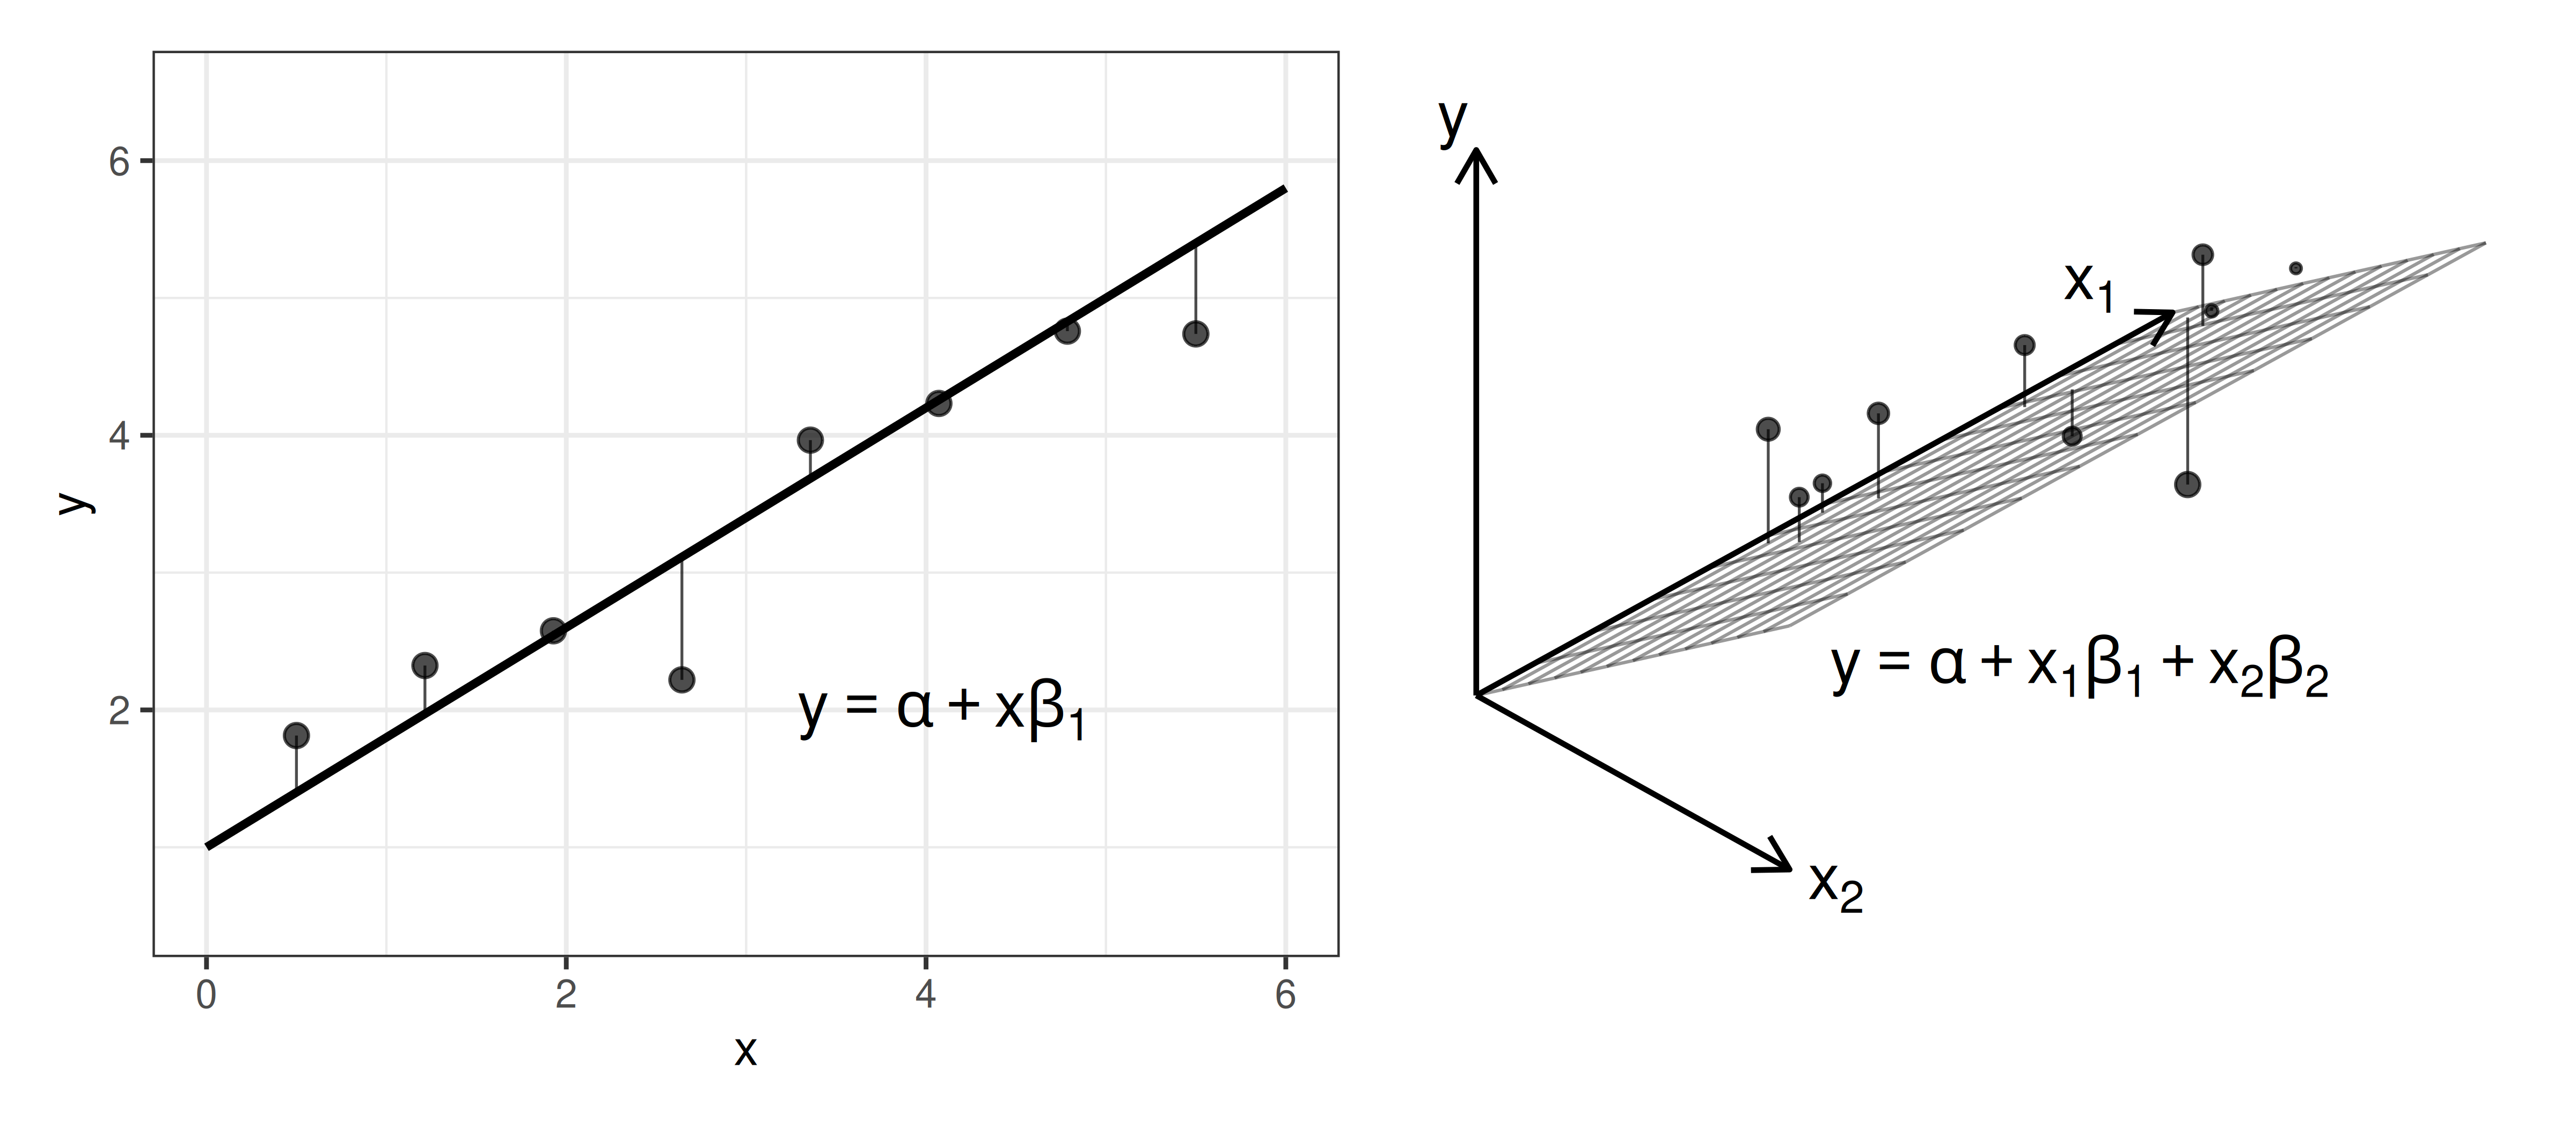
\includegraphics[width=0.9\linewidth,height=\textheight,keepaspectratio]{Figures/svm/fig-p3c15-hyperplane.png}

}

\caption{\label{fig-p3c15-hyperplane}Visualizing hyperplanes as
prediction surfaces. With one predictor (left), the fitted model is
represented by a line, whereas with two predictors (right) the fitted
model becomes a plane, a special case of a hyperplane. Lines from
observations (dots) to the fitted surface show prediction error.}

\end{figure}%

Continuing the linear regression example, consider a simple model where
the objective is to find the
\(\boldsymbol{\mathbf{\beta}} = ({\beta}_1 \ {\beta}_2 \cdots {\beta}_{p})^\top\)
coefficients that minimize,

\[
\sum^n_{i=1} (g(\mathbf{x}_i \mid \boldsymbol{\theta}) - y_i)^2,
\]

where,

\[
g(\mathbf{x}_i \mid \boldsymbol{\theta}) = \alpha + \mathbf{x}_i^\top\boldsymbol{\beta}, \quad \boldsymbol{\theta}= (\alpha, \boldsymbol{\beta}),
\]

with covariates \(\mathbf{x}_i \in \mathbb{R}^p\) and outcome
\(y_i \in \mathbb{R}\). In a higher-dimensional space, models with many
coefficients may overfit\index{overfitting} the training data and
perform poorly on new observations. To control this, a penalty term can
be added to shrink coefficient magnitudes and encourage smoother, less
extreme prediction surfaces, commonly of the form:

\begin{equation}\phantomsection\label{eq-penalized}{
\frac{1}{2} \sum^n_{i=1} (g(\mathbf{x}_i \mid \boldsymbol{\theta}) - y_i)^2 + \frac{\xi}{2} \|\boldsymbol{\beta}\|^2,
}\end{equation}

for some penalty term \(\xi \in \mathbb{R}_{\geq 0}\). The first term
minimizes the total squared difference between predictions and observed
outcomes, while the second penalizes large
coefficients.\index{penalization} Larger values of \(\xi\) place greater
emphasis on shrinkage and model simplicity, whereas smaller values
prioritize closer fit to the training data. Minimizing this objective
results in a hyperplane representing the best regularized linear
relationship between covariates and outcomes.

Similarly to linear regression, support vector machines (SVMs) (Cortes
and Vapnik 1995) also fit a hyperplane, \(g\), on given training data,
\(\mathbf{X}\). However, in SVMs, the goal is to fit a flexible,
non-linear hyperplane that minimizes the difference between predictions
and the observed outcomes for \emph{individual} observations. A core
feature of SVMs is that one does not try to fit a hyperplane that makes
perfect predictions as this would overfit the training data. Instead,
SVMs use a regularized error function, which allows incorrect
predictions (errors) for some observations, with the magnitude of error
controlled by an \(\epsilon>0\) hyperparameter, a penalty hyperparameter
\(C\), and slack parameters
\(\boldsymbol{\mathbf{\zeta^\dagger}} = ({\zeta^\dagger}_1 \ {\zeta^\dagger}_2 \cdots {\zeta^\dagger}_{n})^\top\)
and
\(\boldsymbol{\mathbf{\zeta^\ddagger}} = ({\zeta^\ddagger}_1 \ {\zeta^\ddagger}_2 \cdots {\zeta^\ddagger}_{n})^\top\):\index{support vector machines!slack parameters}\index{support vector machines!hyperparameters!epsilon@$\epsilon$}

\begin{equation}\phantomsection\label{eq-svm-opt}{
\begin{aligned}
& \min_{\boldsymbol{\theta}, \boldsymbol{\zeta}^\dagger, \boldsymbol{\zeta}^\ddagger} \frac{1}{2} \|\boldsymbol{\beta}\|^2 + C \sum^n_{i=1}(\zeta^\dagger_i + \zeta_i^\ddagger) \\
& \textrm{subject to}
\begin{dcases}
g(\mathbf{x}_i \mid \boldsymbol{\theta}), & \geq y_i -\epsilon - \zeta^\dagger_i, \\
g(\mathbf{x}_i \mid \boldsymbol{\theta}), & \leq y_i + \epsilon + \zeta_i^\ddagger, \\
\zeta^\dagger_i, \zeta_i^\ddagger, & \geq 0, \\
\forall i = 1,\ldots,n,
\end{dcases}
\end{aligned}
}\end{equation}

where
\(g(\mathbf{x}_i \mid \boldsymbol{\theta}) = \alpha + \mathbf{x}_i^\top\boldsymbol{\beta}\)
for model weights \(\boldsymbol{\beta}\in \mathbb{R}^p\) and
\(\alpha \in \mathbb{R}\) and the same training data,
\((\mathbf{x}_i, y_i)\), as above. Note that the regularization
trade-off controlled by \(\xi\) in (\ref{eq-penalized}) is now
controlled by the \(C\) penalty on the error terms.

If an observation \(i\) lies within the \(\epsilon\)-tube, then by
definition,

\[
y_i - \epsilon \le g(\mathbf{x}_i \mid \boldsymbol{\theta}) \le y_i + \epsilon.
\]

As slack parameters must be non-negative (third constraint), the
individual slack parameters for this observation attain their minimum at
\(\zeta_i^\dagger=\zeta_i^\ddagger=0\). Consequently, observations
within the \(\epsilon\)-tube contribute nothing to the penalty term in
the objective function (\ref{eq-svm-opt}). If every observation fell
within the \(\epsilon\)-tube, then all slack penalties would be zero and
the remaining objective \(\|\boldsymbol{\beta}\|^2/2\) is minimized by
\(\boldsymbol{\beta}= \mathbf{0}\), resulting in a constant (and
uninformative) prediction surface:
\(g(\mathbf{x}_i \mid \hat{\boldsymbol{\theta}}) = \hat{\alpha}\). In
summary, observations within the \(\epsilon\)-tube do not influence
fitting of the optimal prediction surface (though they may constrain the
intercept, \(\hat{\alpha}\)).

The optimization therefore depends entirely on the influential
observations outside the \(\epsilon\)-tube, known as the \emph{support
vectors}.\index{support vector machines!support vectors} For these
observations, the optimization minimizes the individual slack
parameters, \(\zeta_i^\dagger > 0\) or \(\zeta_i^\ddagger > 0\), which
quantify the magnitude of prediction error for each observation. Note
that in the literature, support vectors are usually defined to also
include observations \emph{on} the \(\epsilon\)-tube as well as outside
it, as observations on the boundary still correspond to active
constraints despite having \(\zeta_i^\dagger = \zeta_i^\ddagger = 0\).
The penalty hyperparameter, \(C \in \mathbb{R}_{>0}\), controls the
slack parameters. As \(C\) increases, the number of slack violations
(errors) is encouraged to decrease, which may result in overfitting with
lower bias but higher variance. In contrast, smaller values of \(C\) are
more likely to introduce higher bias but lower variance (Hastie,
Tibshirani, and Friedman 2001). \(C\) should be tuned to control this
trade-off.\index{support vector machines!hyperparameters!C-penalty}

Figure~\ref{fig-p3c15-regression} visualizes a support vector regression
model in two dimensions. Red dots are the observations within the
\(\epsilon\)-tube and blue diamonds are influential support vectors with
some slack parameters visualized.

\begin{figure}

\centering{

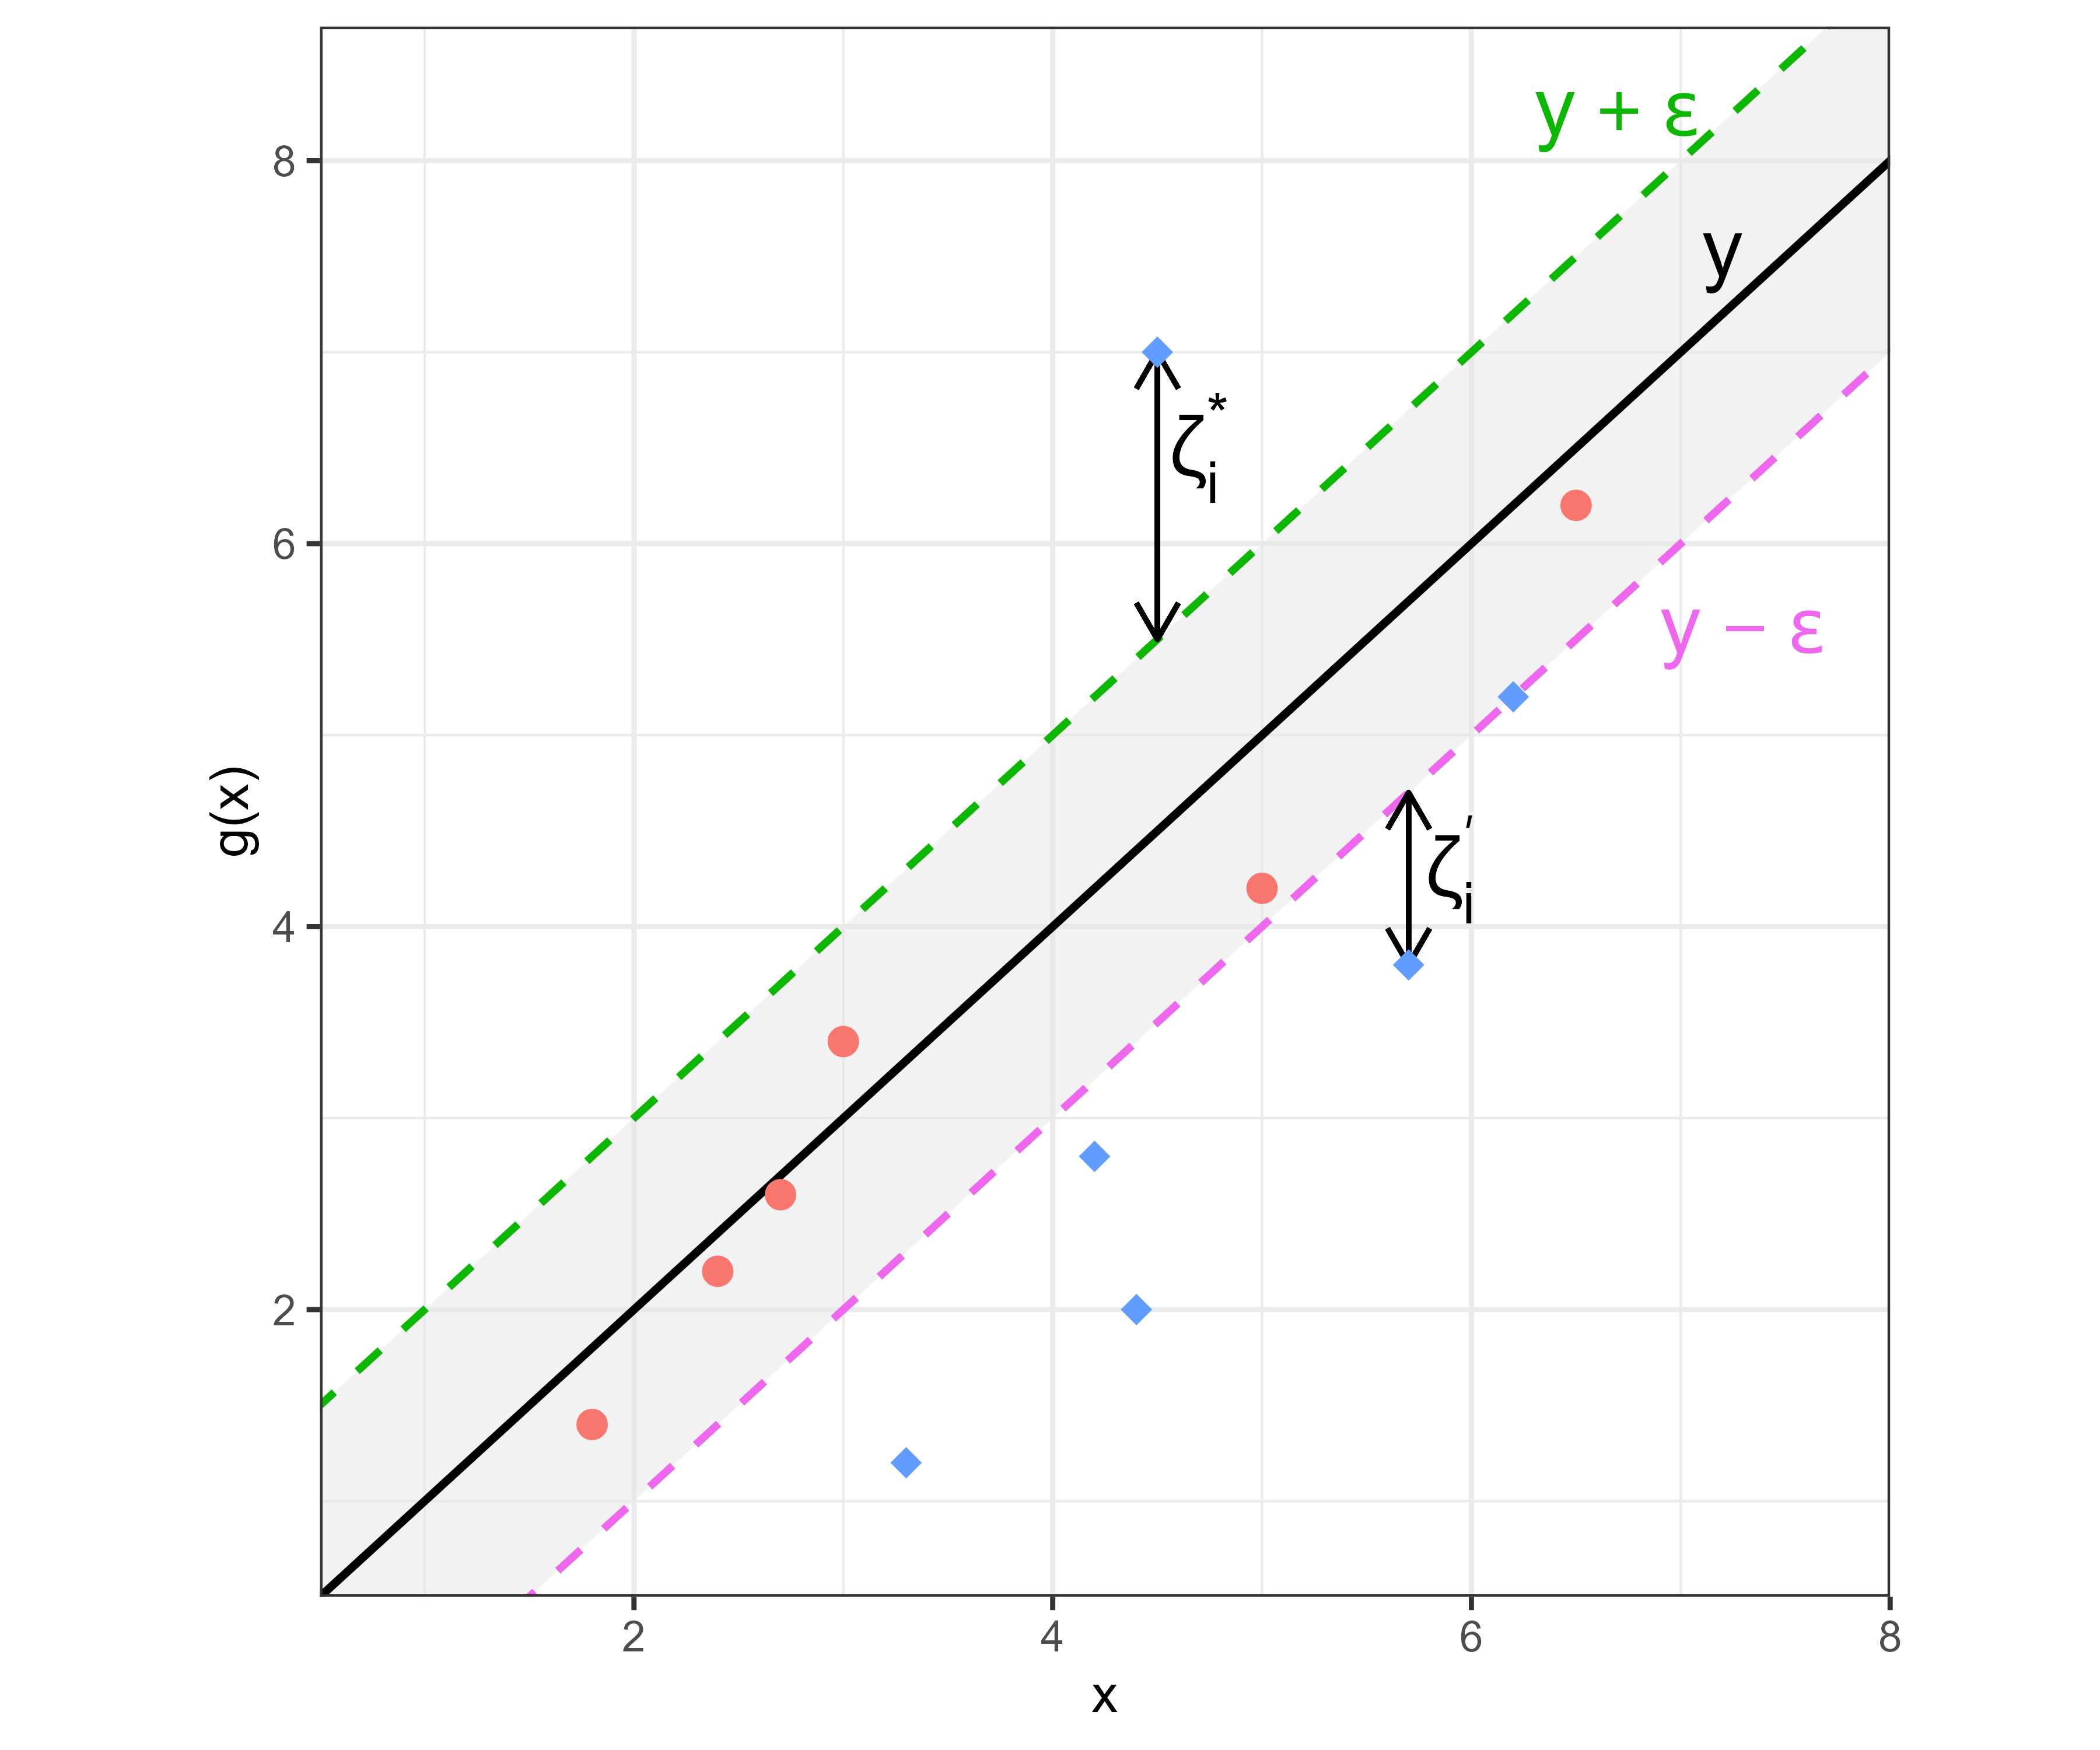
\includegraphics[width=0.6\linewidth,height=\textheight,keepaspectratio]{Figures/svm/fig-p3c15-regression.png}

}

\caption{\label{fig-p3c15-regression}Visualizing a support vector
machine with an \(\epsilon\)-tube (shaded) and slack parameters
\(\boldsymbol{\zeta}\). Red circles are observations within the
\(\epsilon\)-tube and blue diamonds are support vectors outside the
tube. x-axis is single covariate, \(x\), y-axis is the outcome, and the
prediction function is \(g(x) = x\hat{\beta}_1 + \hat{\alpha}\).}

\end{figure}%

The other core feature of SVMs is exploiting the \emph{kernel trick},
which uses functions known as \emph{kernels} to allow the model to learn
a non-linear hyperplane while keeping the computations limited to
lower-dimensional settings.\index{support vector machines!kernels} Once
the model coefficients have been estimated using (\ref{eq-svm-opt}),
predictions for a new observation \(\mathbf{x}_*\) can be made with a
function of the form:

\begin{equation}\phantomsection\label{eq-svm-pred}{
g(\mathbf{x}_* \mid \hat{\boldsymbol{\theta}}) = \sum^n_{i=1} \hat{\mu}_i K(\mathbf{x}_i, \mathbf{x}_*) + \hat{\alpha}.
}\end{equation}

The optimization in (\ref{eq-svm-opt}) is written in its primal form,
where the model is parameterized directly through \(\boldsymbol{\beta}\)
and \(\alpha\). In practice, SVMs are typically estimated using an
equivalent dual formulation based on Lagrange multipliers, \(\mu_i\),
which gives rise to the prediction function in (\ref{eq-svm-pred}). In
this form,
\(\hat{\boldsymbol{\theta}} = (\hat{\boldsymbol{\mu}}, \hat{\alpha})\)
are the estimated dual parameters. The dual formulation absorbs
information from the primal coefficients and slack parameters, replacing
explicit estimation of \(\boldsymbol{\beta}\) and \(\boldsymbol{\zeta}\)
with an equivalent representation based on Lagrange multipliers,
\(\hat{\boldsymbol{\mu}}\), kernels, \(K\), and the intercept,
\(\hat{\alpha}\). In the dual formulation, the support vectors are those
with \(\hat{\mu}_i \ne 0\). Details of estimation of \(\hat{\mu}_i\) are
beyond the scope of this book.

The symbol \(K\) in (\ref{eq-svm-pred}) is a kernel function, with
common choices including
the:\index{support vector machines!kernels!linear}\index{support vector machines!kernels!radial}\index{support vector machines!kernels!polynomial}

\begin{itemize}
\tightlist
\item
  linear kernel:
  \(K(\mathbf{x}_i, \mathbf{x}_*) = \mathbf{x}_i^\top\mathbf{x}_*\);
\item
  radial kernel:
  \(K(\mathbf{x}_i, \mathbf{x}_*) = \exp(-\omega\|\mathbf{x}_i - \mathbf{x}_*\|^2); \quad \omega \in \mathbb{R}_{>0}\);
\item
  polynomial kernel:
  \(K(\mathbf{x}_i, \mathbf{x}_*) = (1 + \mathbf{x}_i^\top\mathbf{x}_*)^d; \quad d \in \mathbb{N}_{> 0}\).
\end{itemize}

The choice of kernel, its parameters, the regularization parameter
\(C\), and the acceptable error \(\epsilon\), are all tunable
hyperparameters (Section~\ref{sec-ml-opt}), which makes the support
vector machine a highly adaptable and often well-performing machine
learning method.\index{hyperparameter} The parameters \(C\) and
\(\epsilon\) often have no clear a priori meaning (especially in the
survival setting, where the rankings are abstract) and thus require
tuning over a wide range of values; inadequate tuning often results in a
poor model fit (Probst, Boulesteix, and Bischl 2019).

\section{SVMs for survival analysis}\label{sec-surv-ml-models-svm-surv}

Extending SVMs to \emph{survival support vector machines} (SSVMs) is a
case of: i) identifying the quantity to predict; and ii) updating the
optimization problem (\ref{eq-svm-opt}) and prediction function
(\ref{eq-svm-pred}) to accommodate
censoring.\index{survival support vector machines} In the first case,
SSVMs can be used to either make survival time or ranking predictions,
which are discussed in turn. The notation above is reused below for
SSVMs, with additional notation introduced when required and now using
the survival training data
\(\{(\mathbf{x}_i, t_i, \delta_i)\}^n_{i=1}\).

\subsection{Survival time SSVMs}\label{survival-time-ssvms}

To begin, consider the objective for support vector regression with the
\(y_i\) variable replaced with the usual outcome time
\(t_i\):\index{survival support vector machines!survival time prediction}

\begin{equation}\phantomsection\label{eq-svm-survnaive}{
\begin{aligned}
& \min_{\boldsymbol{\theta}, \boldsymbol{\zeta}^\dagger, \boldsymbol{\zeta}^\ddagger} \frac{1}{2} \|\boldsymbol{\beta}\|^2 + C_s \sum^n_{i=1}(\zeta^\dagger_i + \zeta_i^\ddagger) \\
& \textrm{subject to}
\begin{dcases}
g(\mathbf{x}_i \mid \boldsymbol{\theta}), & \geq t_i -\epsilon - \zeta^\dagger_i, \\
g(\mathbf{x}_i \mid \boldsymbol{\theta}), & \leq t_i + \epsilon + \zeta_i^\ddagger, \\
\zeta^\dagger_i, \zeta_i^\ddagger, & \geq 0, \\
\forall i = 1,\ldots,n,
\end{dcases}
\end{aligned}
}\end{equation}

where \(C_s \in \mathbb{R}_{>0}\) indicates the penalty parameter
associated with a survival time SSVM.

In survival analysis, this translates to fitting a hyperplane in order
to predict the true survival time. However, as with all adaptations from
regression to survival analysis, there needs to be a method for
incorporating censoring. To do so, consider the first constraint in
(\ref{eq-svm-survnaive}) in isolation,

\[
g(\mathbf{x}_i \mid \boldsymbol{\theta}) \geq t_i - \epsilon - \zeta^\dagger_i,
\]

where the right-hand side is conditioned on the observed outcome time.
In words, this constraint is ensuring the predicted survival time is
greater than some lower bound as a function of the observed outcome time
\(t_i\). For right-censored and uncensored observations, this lower
bound is defined as the right-censoring or true event time respectively.
In contrast, for left-censored observations, there is no informative
lower bound as all that is known is the event occurred at some time
before \(t_i\). Technically, left-censored observations are bounded
below at \(0\), however this lower bound provides little useful
information for constraining predictions at the individual level.

Analogously, the second constraint,

\[
g(\mathbf{x}_i \mid \boldsymbol{\theta}) \leq t_i + \epsilon + \zeta_i^\ddagger,
\]

places an upper bound on the prediction, which is only defined for
left-censored and uncensored observations. In contrast, it is unknown
when a right-censored observation's event actually occurred, so there is
no meaningful upper bound.

Let \(\mathcal{RC}\) be the set of right-censored observations, whose
outcomes are bounded below by the right-censoring time, \(\mathcal{LC}\)
be the set of left-censored observations, with outcomes bounded above by
the left-censoring time, and \(\mathcal{UC}\) be the set of uncensored
observations whose outcomes are bounded above and below by the exact
outcome time. Let \(\mathcal{LB}\) be the set of observations bounded
below,

\[
\mathcal{LB} = \mathcal{RC} \cup \mathcal{UC},
\]

and \(\mathcal{UB}\) be the set of observations bounded above,

\[
\mathcal{UB} = \mathcal{LC} \cup \mathcal{UC}.
\]

These definitions lead to the following optimization problem
(Figure~\ref{fig-p3c15-survival}) (Shivaswamy, Chu, and Jansche 2007):

\begin{equation}\phantomsection\label{eq-shivaswamy}{
\begin{aligned}
& \min_{\boldsymbol{\theta}, \boldsymbol{\zeta}^\dagger, \boldsymbol{\zeta}^\ddagger} \frac{1}{2}\|\boldsymbol{\beta}\|^2 + C_s\Big(\sum_{i \in \mathcal{LB}} \zeta^\dagger_i + \sum_{i \in \mathcal{UB}} \zeta_i^\ddagger\Big) \\
& \textrm{subject to}
\begin{dcases}
g(\mathbf{x}_i \mid \boldsymbol{\theta}), & \geq t_i -\zeta^\dagger_i, i \in \mathcal{LB}, \\
g(\mathbf{x}_i \mid \boldsymbol{\theta}), & \leq t_i + \zeta^\ddagger_i, i \in \mathcal{UB}, \\
\zeta^\dagger_i \geq 0, \forall i\in \mathcal{LB}; \zeta^\ddagger_i \geq 0, \forall i \in \mathcal{UB}.
\end{dcases}
\end{aligned}
}\end{equation}

In general, SSVMs do not use \(\epsilon\) parameters in order to better
accommodate censoring and to help prevent the same penalization of over-
and under-predictions. If \(\epsilon\) were introduced and if no
observations were censored, then the optimization (\ref{eq-shivaswamy})
simplifies to the regression optimization (\ref{eq-svm-opt}).

In contrast to this formulation, one \emph{could} introduce more
\(\epsilon\) and \(C_s\) parameters to separate between under- and
over-predictions and to separate right- and left-censoring, however this
leads to eight tunable hyperparameters, which is inefficient and may
increase overfitting (Fouodo et al. 2018; Land et al. 2011).

If only right-censoring is present in the data then the algorithm can be
simplified by removing the second constraint completely for anyone
censored:

\begin{equation}\phantomsection\label{eq-shivaswamy-right}{
\begin{aligned}
& \min_{\boldsymbol{\theta}, \boldsymbol{\zeta}^\dagger, \boldsymbol{\zeta}^\ddagger} \frac{1}{2}\|\boldsymbol{\beta}\|^2 + C_s \sum_{i = 1}^n (\zeta^\dagger_i + \zeta_i^\ddagger) \\
& \textrm{subject to}
\begin{dcases}
g(\mathbf{x}_i \mid \boldsymbol{\theta}), & \geq t_i - \zeta^\dagger_i, \\
g(\mathbf{x}_i \mid \boldsymbol{\theta}), & \leq t_i + \zeta^\ddagger_i, i:\delta_i=1, \\
\zeta^\dagger_i, \zeta_i^\ddagger, & \geq 0, \\
\forall i = 1,\ldots,n.
\end{dcases}
\end{aligned}
}\end{equation}

With the prediction for a new observation \(\mathbf{x}_*\) calculated
as,

\[
\hat{g}(\mathbf{x}_* \mid \hat{\boldsymbol{\theta}}) = \sum^n_{i=1} \left[\hat{\mu}_i^\dagger K(\mathbf{x}_i, \mathbf{x}_*) - \delta_i\hat{\mu}_i^\ddagger K(\mathbf{x}_i, \mathbf{x}_*)\right] + \hat{\alpha},
\]

where again \(K\) is a kernel function and
\(\hat{\mu}_i^\dagger, \hat{\mu}_i^\ddagger\) are Lagrange multipliers.

\begin{figure}

\centering{

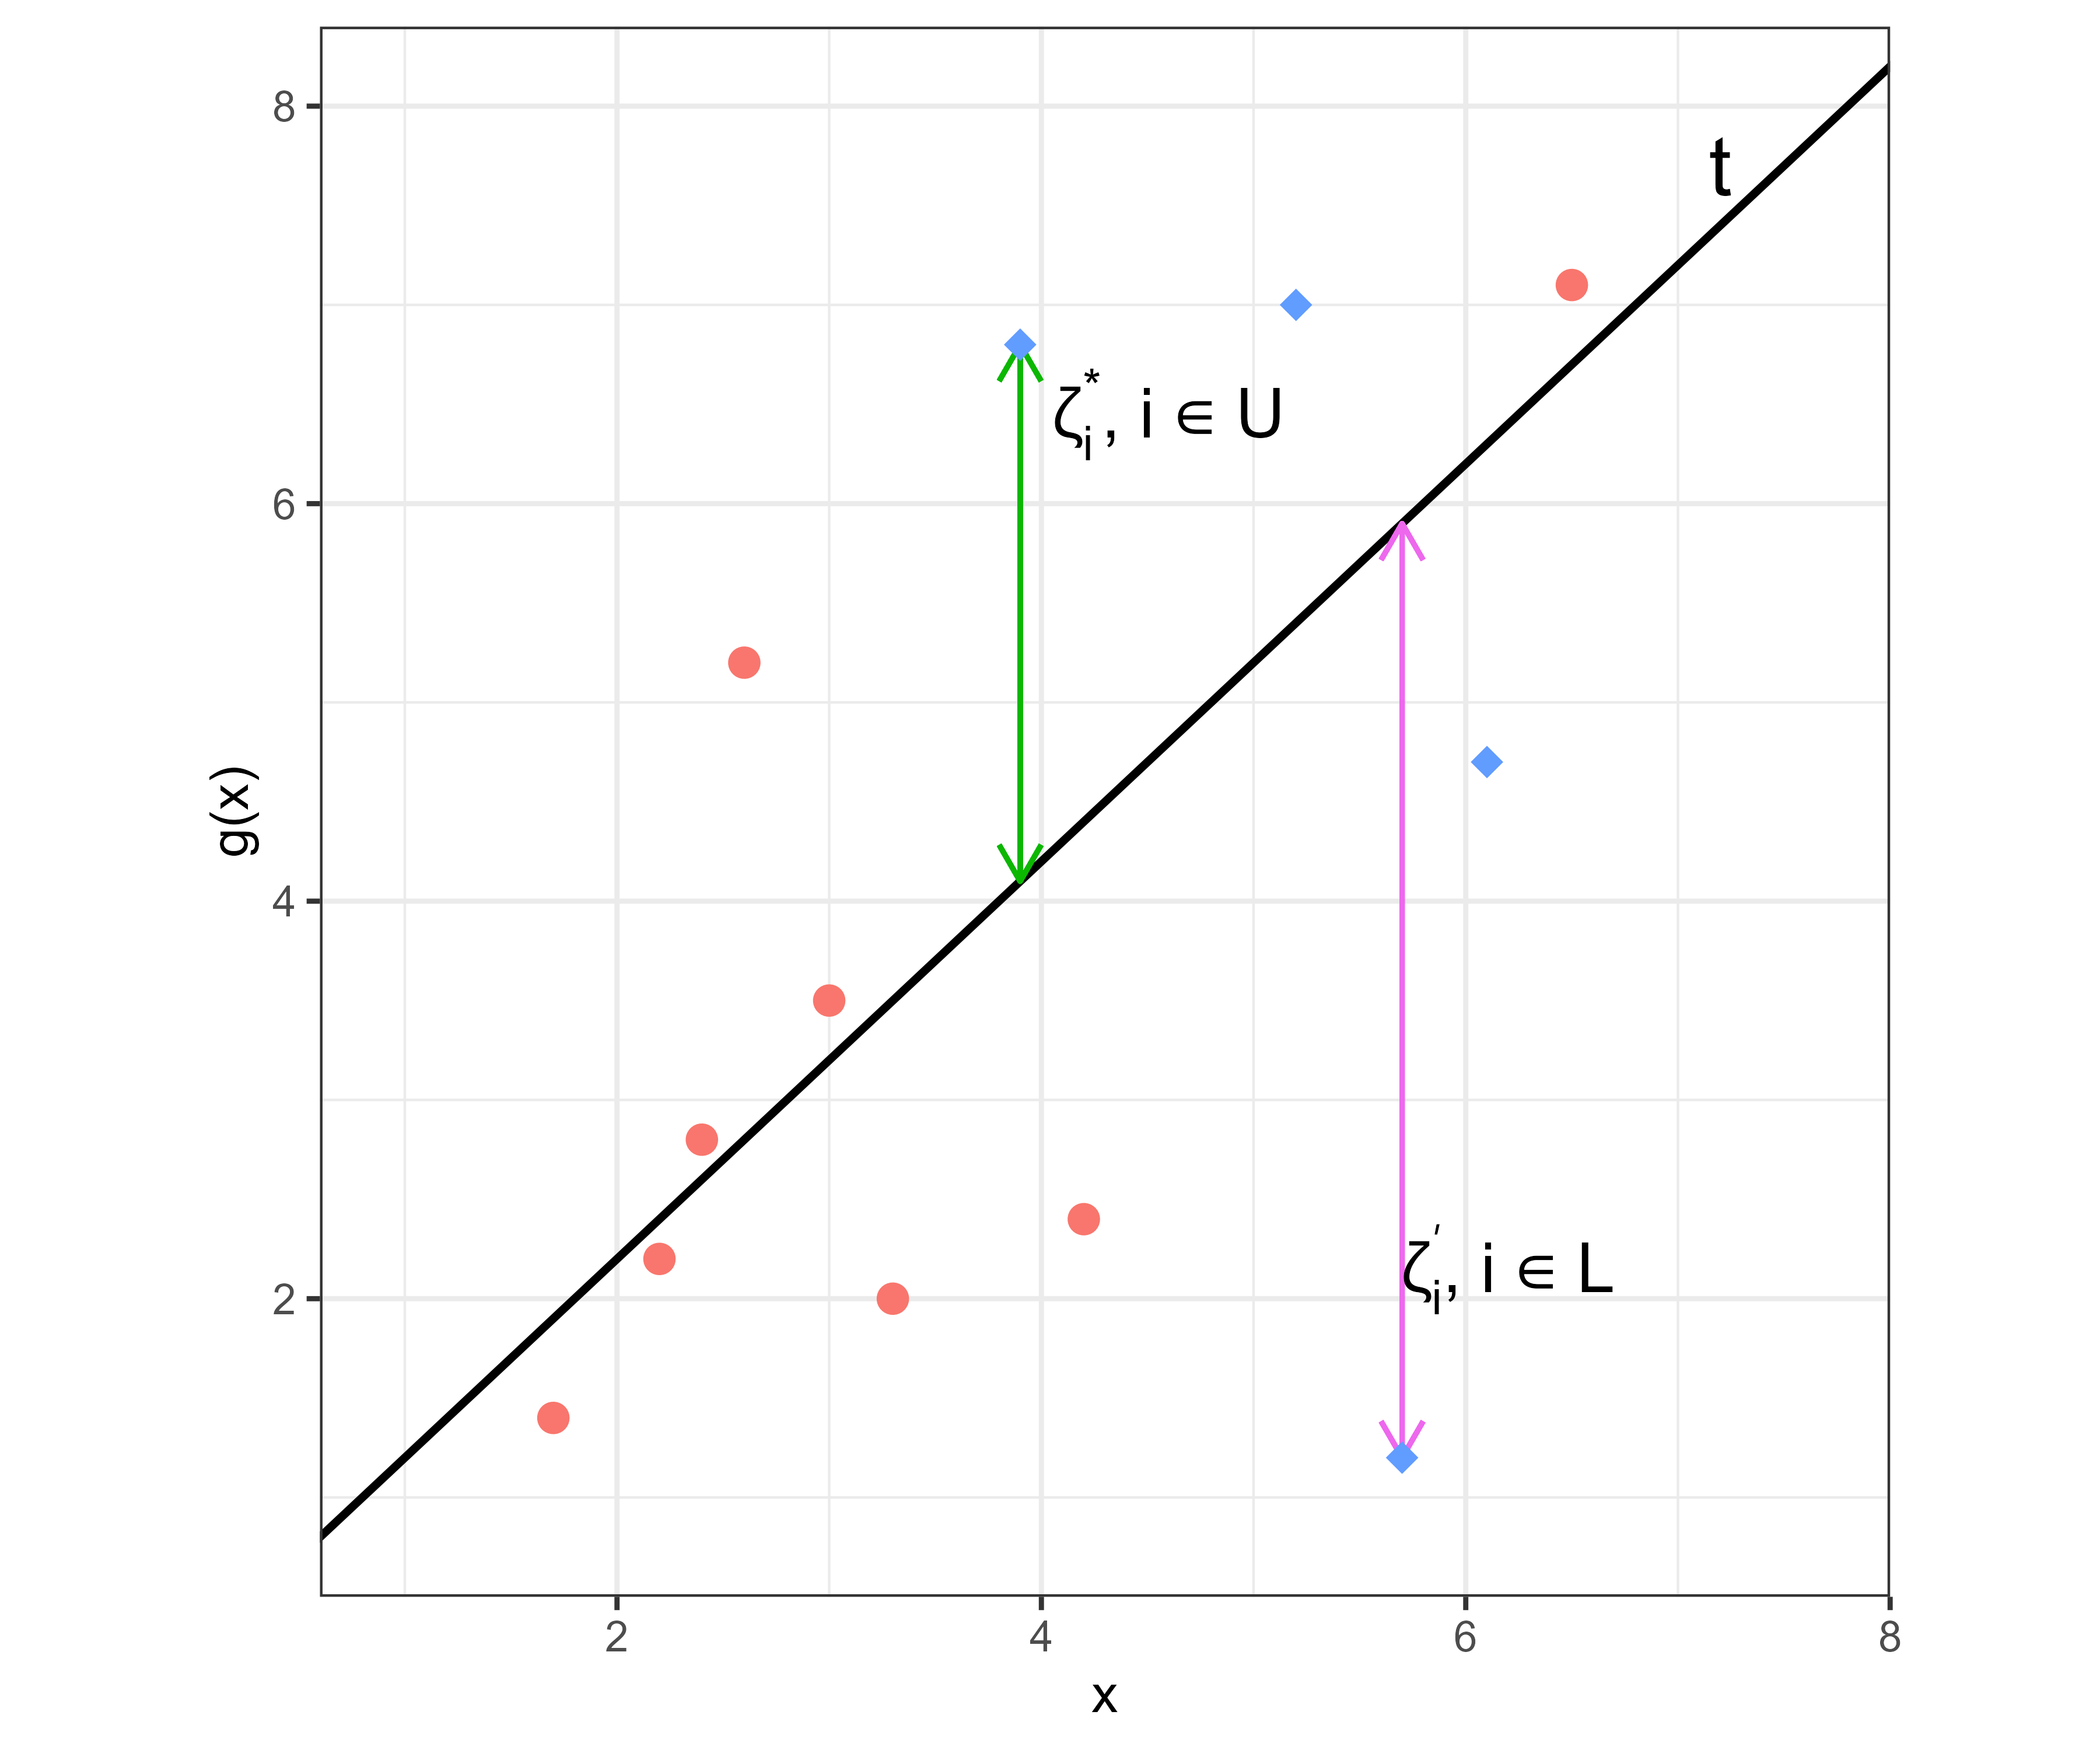
\includegraphics[width=0.6\linewidth,height=\textheight,keepaspectratio]{Figures/svm/fig-p3c15-survival.png}

}

\caption{\label{fig-p3c15-survival}Visualizing a survival time SVM. Blue
diamonds are influential support vectors, which must be those that are
upper bounded (uncensored or left-censored) when \(g(\mathbf{x})>t\), or
lower bounded (uncensored or right-censored) when \(g(\mathbf{x})<t\).
Red circles are non-influential observations.}

\end{figure}%

\subsection{Ranking SSVMs}\label{ranking-ssvms}

Support vector machines can be used to estimate rankings by penalizing
predictions that result in disconcordant
pairs.\index{survival support vector machines!risk prediction} Recall
the definition of concordance from Chapter~\ref{sec-eval-crank}: a pair
of observations \((i, j)\) is comparable if
\(t_i < t_j \wedge \delta_i = 1\), and concordant if \(r_i > r_j\) where
\(r_i, r_j\) are the predicted ranks for observations \(i\) and \(j\)
respectively and a higher value implies greater
risk.\index{concordant pairs} Using the prognostic index as a ranking
prediction (Section~\ref{sec-survtsk-PI}), a pair of observations is
concordant if \(g(\mathbf{x}_i) > g(\mathbf{x}_j)\) when \(t_i < t_j\),
leading to (Van Belle et al. 2007,
2008):\index{survival support vector machines!comparable pairs}

\begin{equation}\phantomsection\label{eq-vanbelle-rank}{
\begin{aligned}
& \min_{\boldsymbol{\theta}, \boldsymbol{\zeta}} \frac{1}{2}\|\boldsymbol{\beta}\|^2 + C_r\sum_{(i,j) \in \mathcal{CP}} \zeta_{ij} \\
& \textrm{subject to}
\begin{dcases}
g(\mathbf{x}_i \mid \boldsymbol{\theta}) - g(\mathbf{x}_j \mid \boldsymbol{\theta}), & \geq 1 - \zeta_{ij}, \\
\zeta_{ij}, & \geq 0, \\
\forall (i,j) \in \mathcal{CP},
\end{dcases}
\end{aligned}
}\end{equation}

where \(\mathcal{CP}\) is the set of comparable pairs defined by
\(\mathcal{CP} = \{(i, j) : t_i < t_j \wedge \delta_i = 1\}\), and
\(C_r \in \mathbb{R}_{>0}\) indicates the penalty parameter associated
with a ranking SSVM. The addition of the constant \(1\) in the first
constraint defines the SSVM margin between comparable observations. The
value \(1\) itself is arbitrary and conventional, as the overall scale
is absorbed by the model coefficients, slack parameters, and
hyperparameters. The constraint encourages not only correct ordering but
also a minimum separation between comparable predictions.

Given that the number of possible pairs grows quadratically with the
number of observations, the optimization problem
(\ref{eq-vanbelle-rank}) quickly becomes difficult to solve with high
computational cost. One solution is a nearest neighbor approach that
sorts observations in order of outcome time and then compares each data
point \(i\) with the observation that has the next smallest
\emph{survival} time, skipping over censored observations (Van Belle et
al. 2008, 2011):

\begin{equation}\phantomsection\label{eq-vb-neighbor}{
j(i) := \mathop{\mathrm{arg\,max}}_{j = 1,\ldots,n} \{t_j : t_j < t_i \wedge \delta_j = 1\}.
}\end{equation}

This is visualized in Figure~\ref{fig-p3c15-comparable} where six
observations are sorted by outcome time from largest (right) to smallest
(left). From right to left, the first pair is made by matching the
observation to the first uncensored outcome to the left, this continues
to the end. In implementation, to ensure all observations are used in
the optimization, the algorithm sets the first outcome to be uncensored;
hence observation \(2\) being compared to observation \(1\) in
Figure~\ref{fig-p3c15-comparable}.

\begin{figure}

\centering{

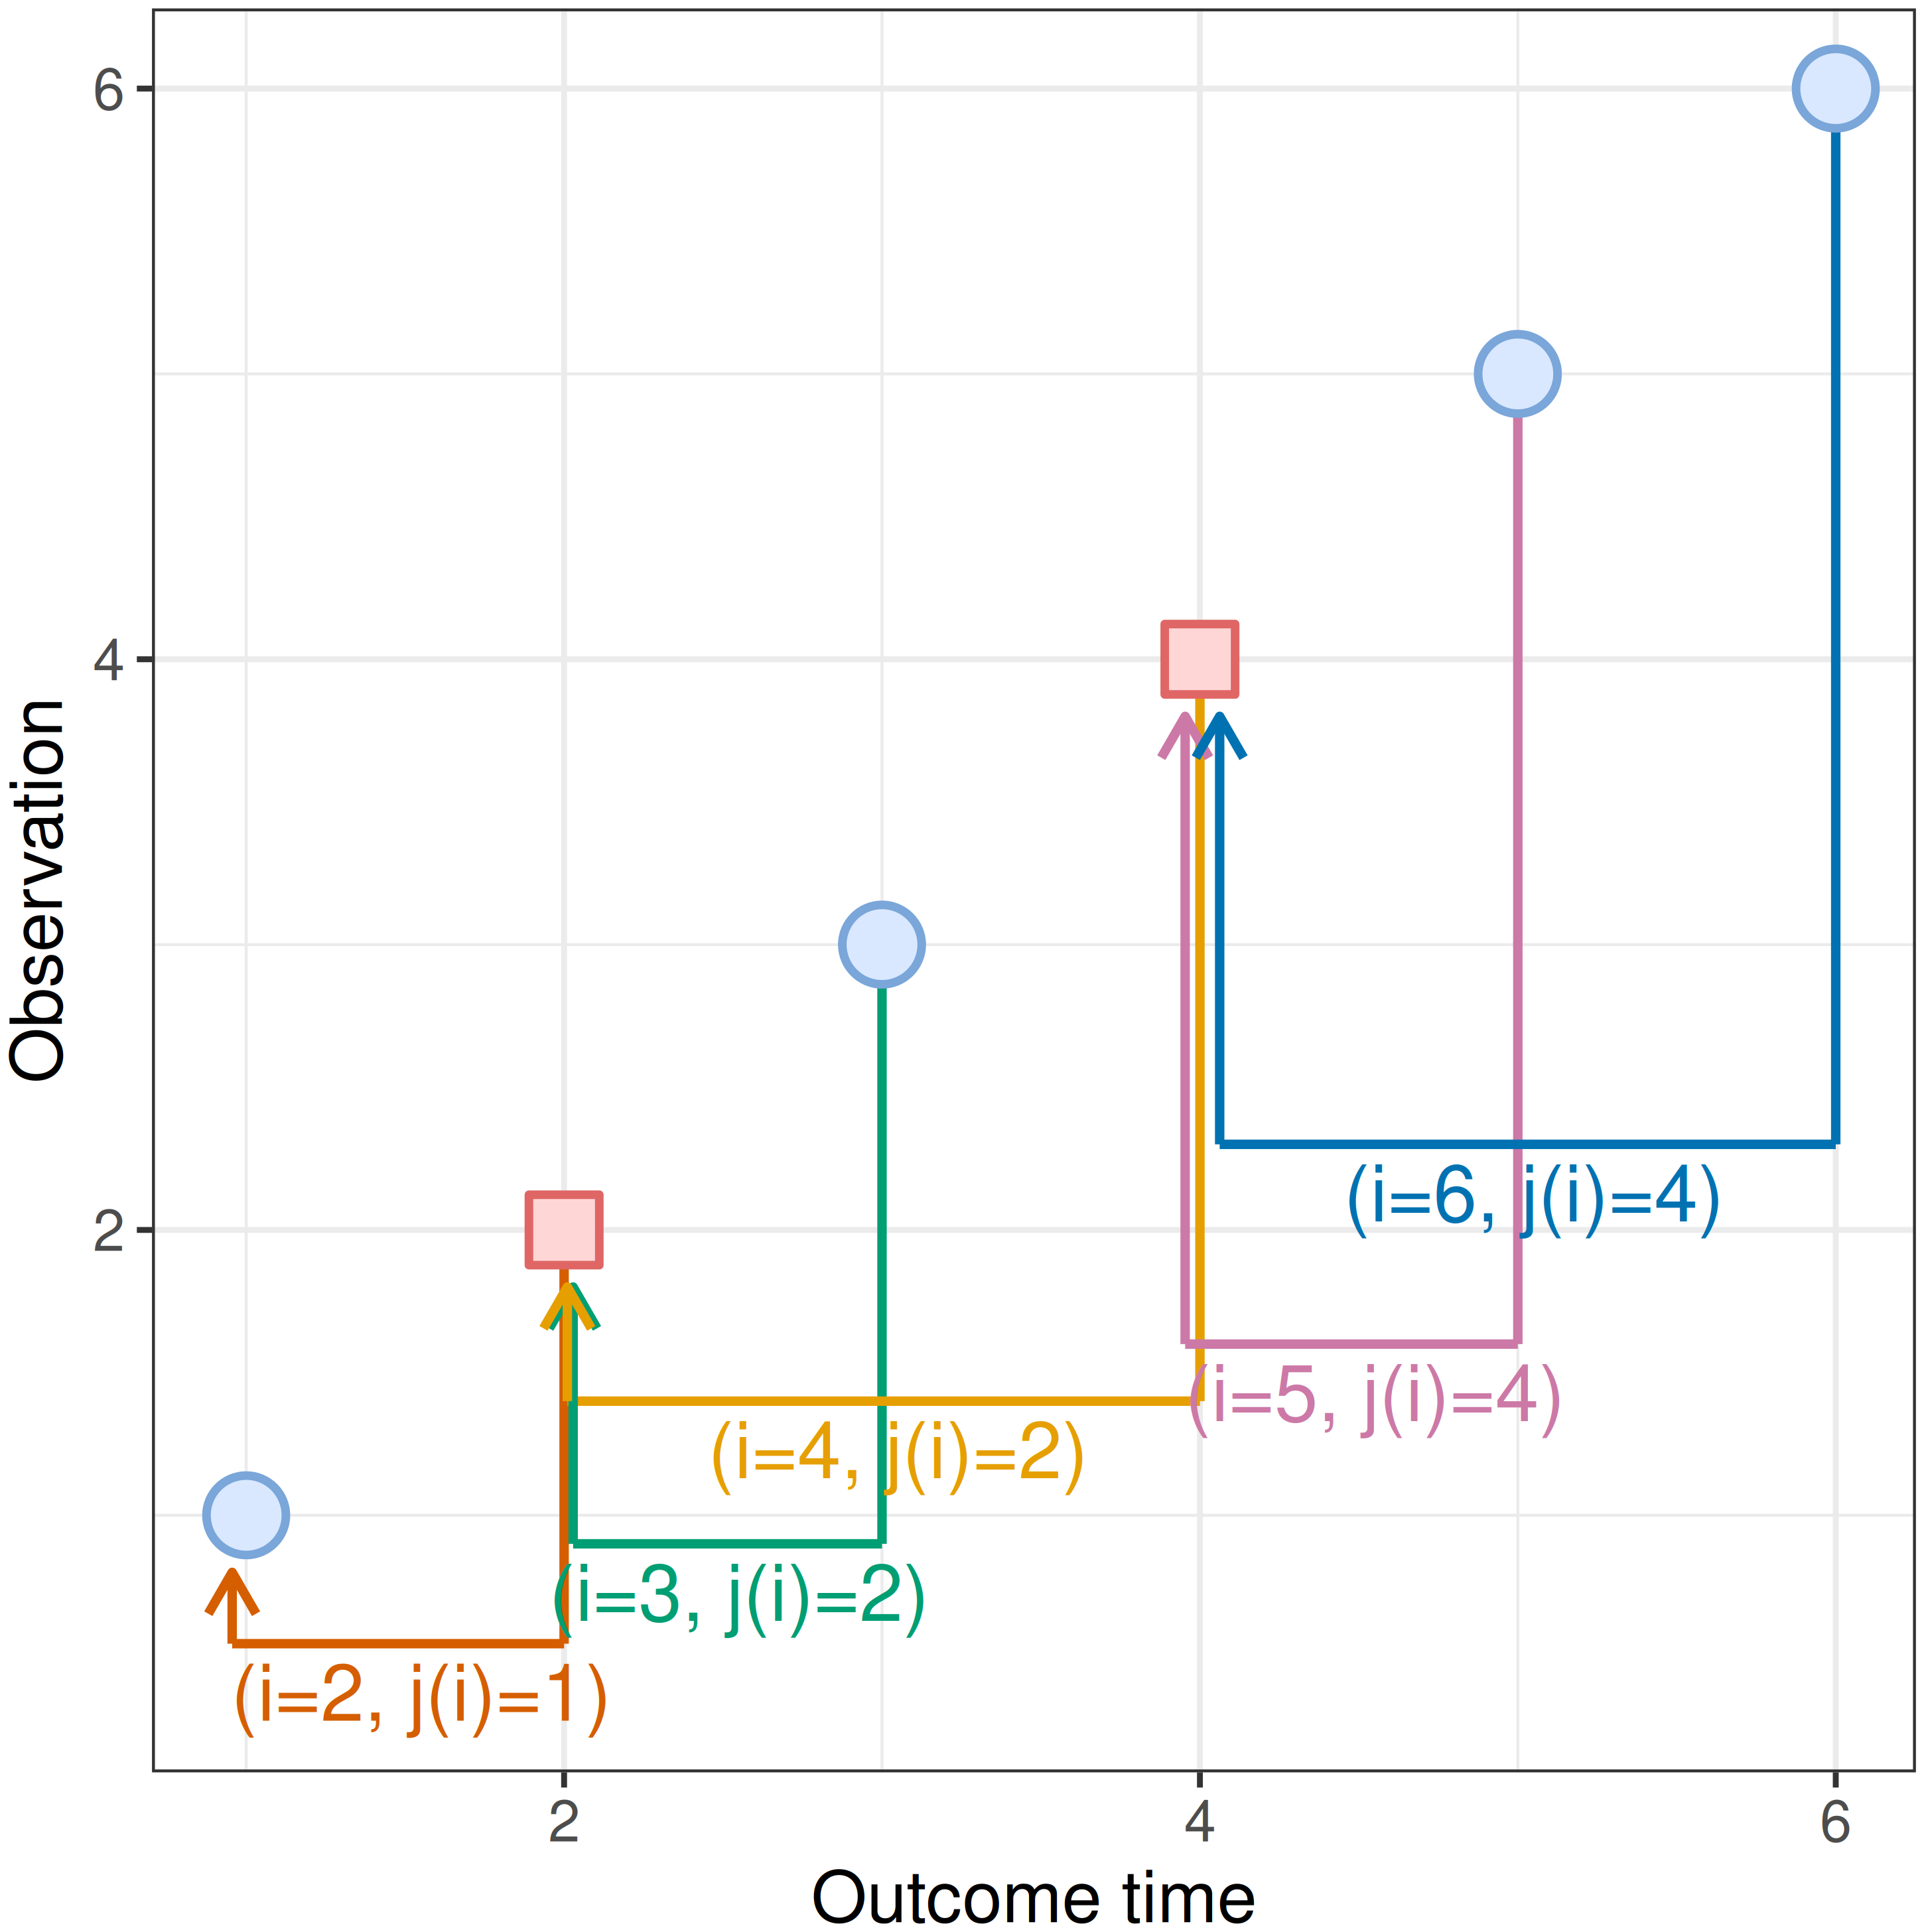
\includegraphics[width=0.6\linewidth,height=\textheight,keepaspectratio]{Figures/svm/fig-p3c15-comparable.png}

}

\caption{\label{fig-p3c15-comparable}Van Belle SVM nearest neighbors
approach for comparable pairs. Sorted observations are paired with the
nearest uncensored outcome `to the left'. Red squares are uncensored
observations and blue circles are censored. The observation with the
smallest outcome time is always treated as uncensored.}

\end{figure}%

Using this method, the algorithm becomes:

\begin{equation}\phantomsection\label{eq-ssvm-rank}{
\begin{aligned}
& \min_{\boldsymbol{\theta}, \boldsymbol{\zeta}} \frac{1}{2}\|\boldsymbol{\beta}\|^2 + C_r\sum_{i =1}^n \zeta_i \\
& \textrm{subject to}
\begin{dcases}
g(\mathbf{x}_{j(i)}) - g(\mathbf{x}_i \mid \boldsymbol{\theta}), & \geq t_i - t_{j(i)} - \zeta_i, \\
\zeta_i, & \geq 0, \\
\forall i = 1,\ldots,n.
\end{dcases}
\end{aligned}
}\end{equation}

Note that \(j(i)\) is defined in (\ref{eq-vb-neighbor}) so that
\(t_{j(i)} < t_i\). Under the convention that larger values of
\(g(\mathbf{x})\) imply greater risk, the constraint in
(\ref{eq-ssvm-rank}) requires
\(g(\mathbf{x}_{j(i)}) - g(\mathbf{x}_i) > 0\) (thus,
\(g(\mathbf{x}_{j(i)}) > g(\mathbf{x}_i)\)) whenever the slack term,
\(\zeta_i\), is sufficiently small as \(t_i - t_{j(i)} > 0\). The
updated right-hand side of the constraint defines a margin that
increases with the difference in observed outcome times, while the slack
term, \(\zeta_i\), captures violations beyond this difference.

Predictions for a new observation \(\mathbf{x}_*\) are calculated as,

\[
g(\mathbf{x}_* \mid \hat{\boldsymbol{\theta}}) = \sum^n_{i=1} \hat{\mu}_i(K(\mathbf{x}_{j(i)}, \mathbf{x}_*) - K(\mathbf{x}_i, \mathbf{x}_*)) + \hat{\alpha},
\]

where \(\hat{\mu}_i\) are again Lagrange multipliers.

There do not appear to be any adaptations to the ranking SSVM for other
censoring or truncation types.

\subsection{Hybrid SSVMs}\label{hybrid-ssvms}

Finally, Van Belle et al. (2011) noted that the ranking algorithm could
be updated to add the constraints of the survival time model, thus
providing a model that simultaneously optimizes for ranking while
providing continuous values that can be interpreted as survival time
predictions. This results in the hybrid
SSVM:\index{survival support vector machines!hybrid prediction}

\[
\begin{aligned}
& \min_{\boldsymbol{\theta}, \boldsymbol{\zeta}, \boldsymbol{\zeta}^\dagger, \boldsymbol{\zeta}^\ddagger} \frac{1}{2}\|\boldsymbol{\beta}\|^2 + \textcolor{CornflowerBlue}{C_r\sum_{i =1}^n \zeta_i} + \textcolor{Rhodamine}{C_s \sum^n_{i=1}(\zeta_i^\dagger + \zeta_i^\ddagger)} \\
& \textrm{subject to}
\begin{dcases}
\textcolor{CornflowerBlue}{-(g(\mathbf{x}_{j(i)} \mid \boldsymbol{\theta}) - g(\mathbf{x}_i \mid \boldsymbol{\theta}))}, & \textcolor{CornflowerBlue}{\geq t_i - t_{j(i)} - \zeta_i}, \\
\textcolor{Rhodamine}{g(\mathbf{x}_i \mid \boldsymbol{\theta})}, & \textcolor{Rhodamine}{\leq t_i + \zeta^\ddagger_i, i:\delta_i=1}, \\
\textcolor{Rhodamine}{g(\mathbf{x}_i \mid \boldsymbol{\theta})}, & \textcolor{Rhodamine}{\geq t_i - \zeta^\dagger_i}, \\
\textcolor{CornflowerBlue}{\zeta_i}, \textcolor{Rhodamine}{\zeta_i^\dagger, \zeta_i^\ddagger}, & \geq 0, \\
\forall i = 1,\ldots,n.
\end{dcases}
\end{aligned}
\]

The blue parts of the equation make up the ranking model and the red
parts are the survival time model. Note the addition of the negative
sign in the first constraint, which is required to ensure larger values
of \(g\) correspond to both longer survival times and lower risk.

Setting \(C_r = 0\) recovers the survival time SSVM
(\ref{eq-shivaswamy-right}), while setting \(C_s = 0\) recovers the
ranking SSVM (\ref{eq-ssvm-rank}) up to a sign reversal. Hence, fitting
the hybrid model and tuning these parameters is an efficient way to
automatically detect which SSVM is best suited to a given task.

Once the model is fit, a prediction from given features
\(\mathbf{x}_* \in \mathbb{R}^p\), can be made using the equation below,
again with the ranking and survival time contributions highlighted in
blue and red respectively.

\[
\hat{g}(\mathbf{x}_* \mid \hat{\boldsymbol{\theta}}) = \sum^n_{i=1} \left[\textcolor{CornflowerBlue}{-\hat{\mu}_i(K(\mathbf{x}_{j(i)}, \mathbf{x}_*) - K(\mathbf{x}_i, \mathbf{x}_*))} + \textcolor{Rhodamine}{\hat{\mu}^\dagger_i K(\mathbf{x}_i, \mathbf{x}_*) - \delta_i\hat{\mu}_i^\ddagger K(\mathbf{x}_i, \mathbf{x}_*)}\right] + \hat{\alpha}
\]

where \(\hat{\mu}_i, \hat{\mu}_i^\dagger, \hat{\mu}_i^\ddagger\) are
Lagrange multipliers and \(K\) is a chosen kernel function, which may
have further hyperparameters to select or tune.

\subsection{Competing risks}\label{competing-risks-2}

As of the time of publication, no SSVMs for competing risks appear to
have been published (Djangang, Han, and Sanyal 2025; Kantidakis et al.
2023; Monterrubio-Gómez, Constantine-Cooke, and Vallejos
2024).\index{survival support vector machines!competing risks} As
discussed in Section~\ref{sec-survtsk-time}, there is not a
straightforward concept of time-to-event competing risks predictions so
survival time SSVMs are unlikely to be extended to competing risks. For
the ranking SSVMs, theoretically one could use any of the methods to
estimate per-cause risk by considering each risk separately and
censoring observations that experience a different risk, however this
has not been validated in the literature. Moreover, the risks predicted
by SSVMs correspond to abstract relative risks and not to an
interpretable hazard, meaning there is no clear method to transform
these predictions into a CIF or any other distribution-defining function
(Section~\ref{sec-survtsk-risk}). Theoretically, one could consider a
transformation based on survival time predictions; however, this
approach also does not appear to have been explored in the literature.

\section{Conclusion}\label{conclusion-10}

\begin{tcolorbox}[enhanced jigsaw, toprule=.15mm, bottomtitle=1mm, opacityback=0, breakable, leftrule=.75mm, title={Key takeaways}, toptitle=1mm, bottomrule=.15mm, colback=white, colframe=quarto-callout-warning-color-frame, titlerule=0mm, opacitybacktitle=0.6, coltitle=black, rightrule=.15mm, left=2mm, colbacktitle=quarto-callout-warning-color!10!white, arc=.35mm]

\begin{itemize}
\tightlist
\item
  Support vector machines (SVMs) are a highly flexible machine learning
  method that can use the `kernel trick' to implicitly represent high-
  or infinite-dimensional feature spaces while computing in the original
  input space.
\item
  Survival SVMs (SSVMs) extend regression SVMs by either making survival
  time predictions, ranking predictions, or a combination of the two.
\item
  The hybrid SSVM provides an efficient method that encapsulates all the
  elements of survival time and ranking SSVMs and is therefore a good
  model to include in benchmark experiments to test the potential of
  SSVMs.
\item
  SSVMs can only perform well with extensive tuning of hyperparameters
  over a wide parameter space. To date, published guidance on tuning
  ranges for \(C_r\) and \(C_s\) appears limited, though (Fouodo et al.
  2018) tune over \((2^{-5}, 2^5)\).
\end{itemize}

\end{tcolorbox}

\begin{tcolorbox}[enhanced jigsaw, toprule=.15mm, bottomtitle=1mm, opacityback=0, breakable, leftrule=.75mm, title={Further reading}, toptitle=1mm, bottomrule=.15mm, colback=white, colframe=quarto-callout-tip-color-frame, titlerule=0mm, opacitybacktitle=0.6, coltitle=black, rightrule=.15mm, left=2mm, colbacktitle=quarto-callout-tip-color!10!white, arc=.35mm]

\begin{itemize}
\tightlist
\item
  To learn more about survival time SSVMs: Khan and Bayer Zubek (2008),
  Land et al. (2011), Shivaswamy, Chu, and Jansche (2007), and Van Belle
  et al. (2011).
\item
  For more information about ranking SSVMs: Evers and Messow (2008), Van
  Belle et al. (2007), Van Belle et al. (2008), and Van Belle et al.
  (2011).
\item
  Goli, Mahjub, Faradmal, and Soltanian (2016) and Goli, Mahjub,
  Faradmal, Mashayekhi, et al. (2016) introduce mean residual lifetime
  optimization SSVMs.
\item
  Fouodo et al. (2018) surveys and benchmarks SSVMs.
\end{itemize}

\end{tcolorbox}

\chapter{Gradient Boosting Machines}\label{sec-boost}

Similarly to random forests\index{random forests}, boosting is an
ensemble method that creates a powerful model from a combination of
\emph{weak} learners that make poor predictions
individually.\index{gradient boosting machines}\index{weak learner}
However, the two methods differ in how individual learners are selected
and combined: in random forests, each decision tree is grown
independently and predictions are averaged. In boosting, weak learners
are fit sequentially with errors from one learner used to train the
next, and predictions are made by a weighted linear combination of all
learners (Figure~\ref{fig-p3c16-boosting}).

\section{GBMs for regression}\label{sec-surv-ml-models-boost-regr}

Gradient boosting machines (GBMs) are among the most widely used
families of boosting algorithms. The general idea, inspired by gradient
descent (Section~\ref{sec-ml-gradient-descent}), is to choose a
differentiable loss function and iteratively improve predictions by
fitting weak learners to the remaining errors from the current model.
These errors correspond to the negative gradients, or
pseudo-residuals.\index{pseudo-residuals}
Figure~\ref{fig-p3c16-boosting} illustrates this process in a
least-squares regression setting, where the negative gradient
corresponds to the ordinary residual, which is the observed outcome
minus the current prediction.\index{gradient descent} This procedure can
be understood as follows:

\begin{enumerate}
\def\labelenumi{\arabic{enumi}.}
\tightlist
\item
  An initial, simple model is fit to the data to obtain the first set of
  predictions.
\item
  The errors of this model are computed by comparing predictions to the
  observed outcomes.
\item
  A weak learner is fit to these errors, focusing on patterns that the
  previous model failed to capture.
\item
  The new learner is added to the existing model, improving the overall
  prediction.
\item
  This is repeated with each learner correcting the errors of the
  current model.
\end{enumerate}

Predictions are therefore built up gradually as a sum of many weak
learners, each making a small contribution to the final model.

\begin{figure}

\centering{

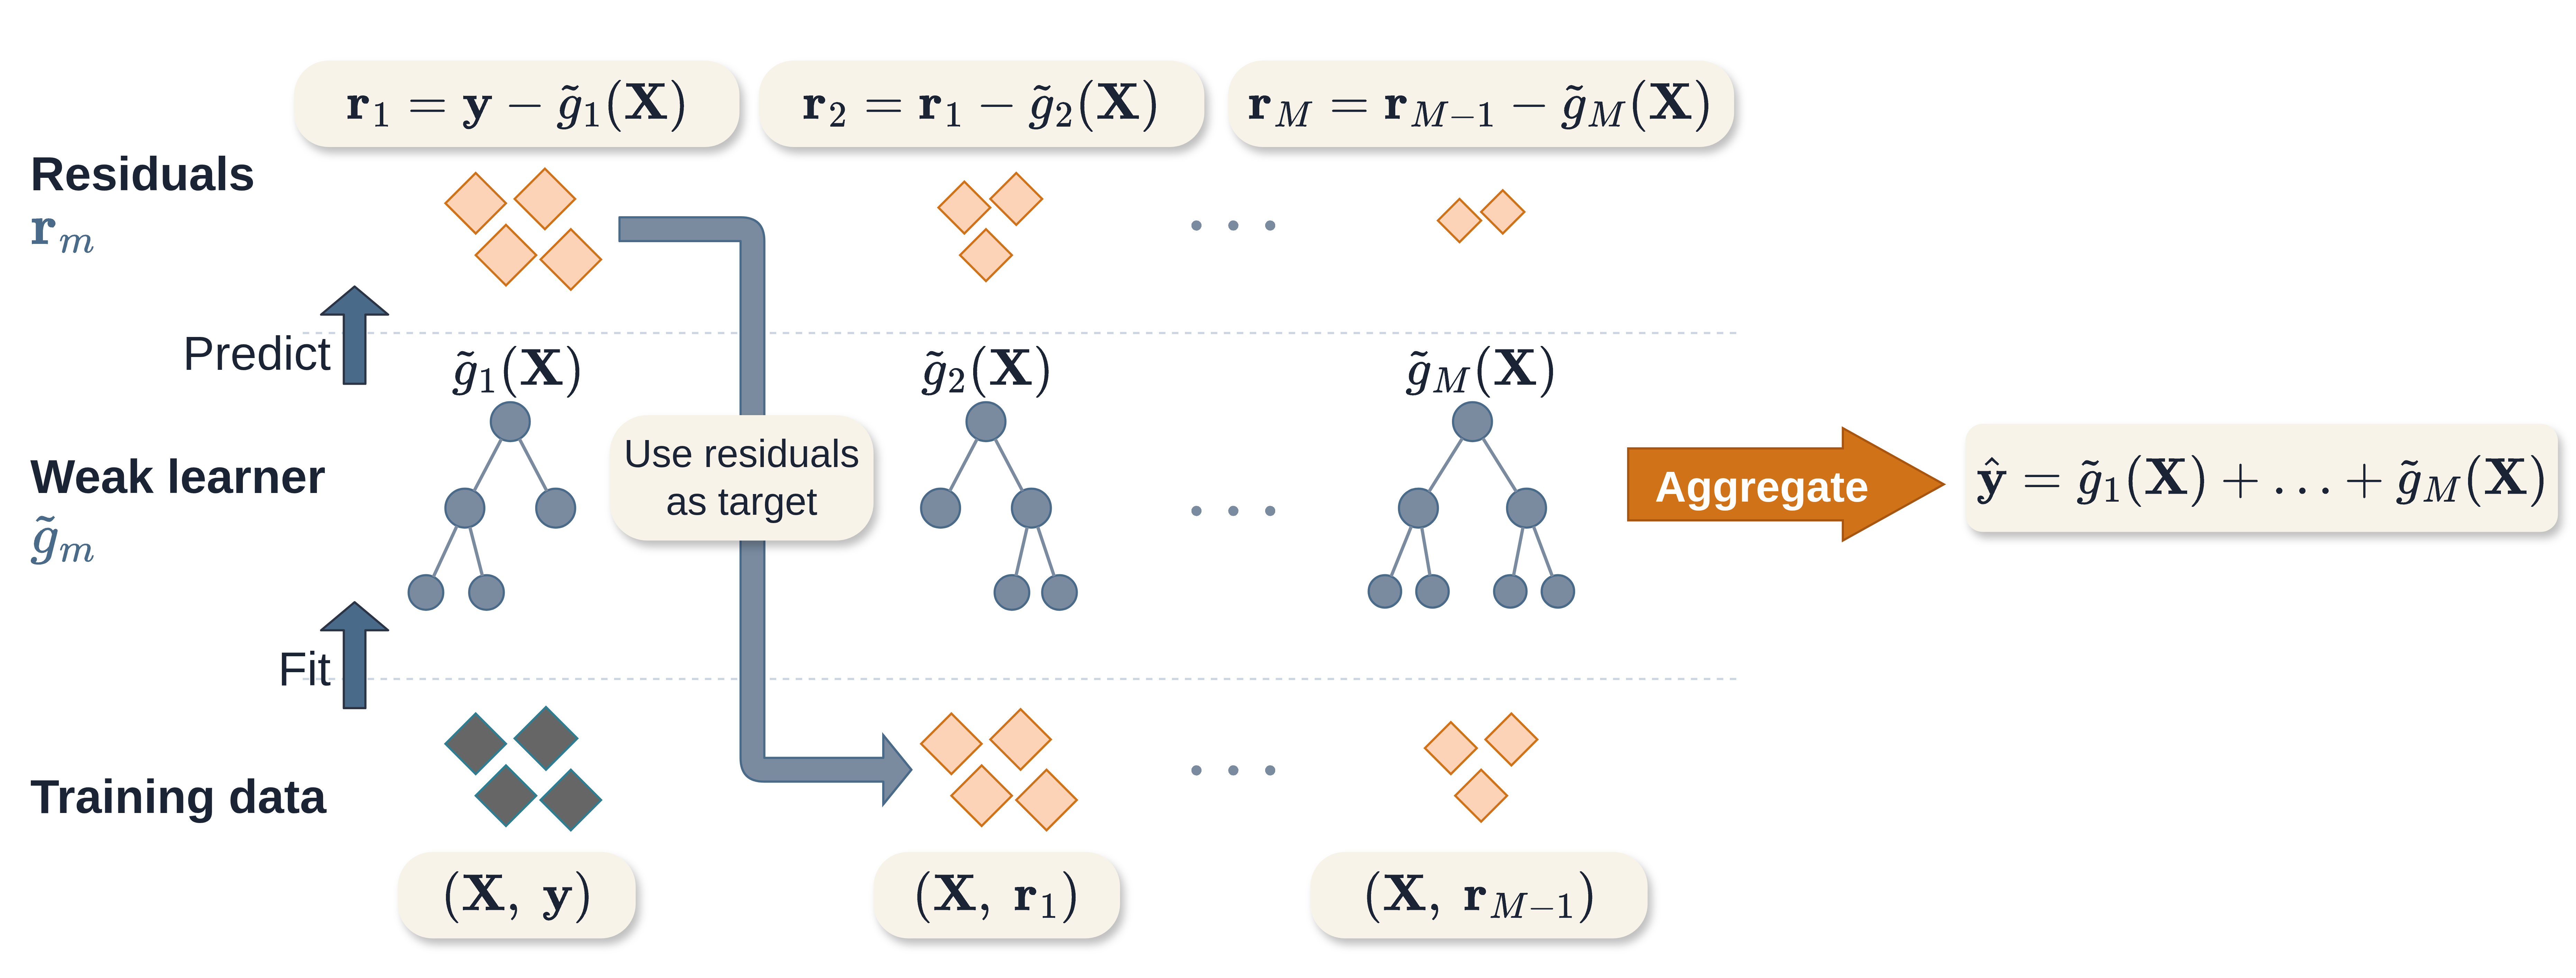
\includegraphics[width=0.9\linewidth,height=\textheight,keepaspectratio]{Figures/boosting/fig-p3c16-boosting.png}

}

\caption{\label{fig-p3c16-boosting}Least squares gradient boosting,
where each weak learner (here, a decision tree) is fit to the residuals
(negative gradient of squared error loss).}

\end{figure}%

Practically, a number of important hyperparameters are used to control
and optimize the algorithm while reducing
overfitting.\index{gradient boosting machines!hyperparameters} These
are:

\textbf{Number of iterations},
\(M\):\index{gradient boosting machines!hyperparameters!iterations} The
number of iterations is often claimed to be the most important
hyperparameter in GBMs and it has been demonstrated that a value too
small will result in underfitting, while a value too large will result
in overfitting (Buhlmann 2006; Hastie, Tibshirani, and Friedman 2001;
Schmid and Hothorn 2008a).\index{overfitting} This underlines the
general idea of boosting weak learners to slowly construct a single
powerful model.

\textbf{Step size},
\(\alpha\):\index{gradient boosting machines!hyperparameters!step size}
The step size parameter is a shrinkage parameter that controls the
contribution of the weak learner at each iteration. Several studies have
demonstrated that GBMs perform better when shrinkage is applied and a
value of \(\alpha \leq 0.1\) is often suggested (Buhlmann and Hothorn
2007; J. H. Friedman 2001; Hastie, Tibshirani, and Friedman 2001; D. K.
K. Lee, Chen, and Ishwaran 2021; Schmid and Hothorn 2008a). The optimal
values of \(\alpha\) and \(M\) depend on each other, such that smaller
values of \(\alpha\) require larger values of \(M\), and vice versa.
This is intuitive as smaller \(\alpha\) results in slower learning and
therefore more iterations are required to fit the model. A practical
procedure is to set \(\alpha\) to a small value (such as \(0.1\)) and
\(M\) to a very large value (such as \(10,\!000\)), then use early
stopping (Section~\ref{sec-ml-early-stopping}) to halt the algorithm
once performance on a validation set stops
improving.\index{early stopping} This avoids the need for
computationally expensive tuning to find the optimal combination of
\(\alpha\) and \(M\).

\textbf{Subsampling proportion},
\(\phi\):\index{gradient boosting machines!hyperparameters!subsampling}
Sampling a fraction, \(\phi\), of the training data at each iteration
can improve performance and reduce runtime (Hastie, Tibshirani, and
Friedman 2001), with \(\phi = 0.5\) often used although ideally it
should be tuned. Motivated by the success of bagging in random forests,
stochastic gradient boosting (J. Friedman 1999) randomly samples the
data in each iteration. Subsampling appears to perform best when
combined with shrinkage (Hastie, Tibshirani, and Friedman 2001).

In addition to these parameters, the hyperparameters of the underlying
weak learner are also commonly tuned. When using decision trees, it is
usual to restrict the number of terminal nodes in the tree to be between
four and eight, corresponding to shallow trees with limited interaction
depth.\index{decision tree} With these hyperparameters and some
differentiable loss \(L\), the general gradient boosting machine
algorithm is given in Algorithm 2.

\begin{tcolorbox}[enhanced jigsaw, toprule=.15mm, bottomtitle=1mm, opacityback=0, breakable, leftrule=.75mm, title={Algorithm 2 (Gradient boosting)}, toptitle=1mm, bottomrule=.15mm, colback=white, colframe=quarto-callout-note-color-frame, titlerule=0mm, opacitybacktitle=0.6, coltitle=black, rightrule=.15mm, left=2mm, colbacktitle=quarto-callout-note-color!10!white, arc=.35mm]

\begin{enumerate}
\def\labelenumi{\arabic{enumi}.}
\tightlist
\item
  \(\hat{g}_0 \gets \text{ Initial guess}\)
\item
  \textbf{for} \(m = 1,\ldots,M\):
\item
  ~~~~~\(\{(\mathbf{x}_i', y_i')\}^{n'}_1 \gets\) Random sample of size
  \(n' = \lfloor \phi n \rfloor\) from \(\{(\mathbf{x}_i, y_i)\}_1^n\)
\item
  ~~~~~\(\displaystyle r_{im} \gets -\frac{\partial L(y'_i, \hat{g}_{m-1}(\mathbf{x}'_i))}{\partial \hat{g}_{m-1}(\mathbf{x}'_i)}, \forall i \in \{1,\ldots,n'\}\)
\item
  ~~~~~\(\tilde{g}_m \gets\) Fit the weak learner to
  \((\mathbf{X}', \mathbf{r}_m)\)
\item
  ~~~~~\(\hat{g}_m \gets \hat{g}_{m-1} + \alpha \tilde{g}_m\)
\item
  \textbf{end for}
\item
  \textbf{return} \(\hat{g}_0, \{\tilde{g}_m\}^M_1\)
\end{enumerate}

Note:

\begin{enumerate}
\def\labelenumi{\arabic{enumi}.}
\tightlist
\item
  \(\tilde{g}_m\) is the weak learner in iteration \(m\) trained on
  pseudo-residuals\index{pseudo-residuals} computed from the cumulative
  model from the previous iteration, \(\hat{g}_{m-1}\). The returned
  object can be written as the final cumulative model, \(\hat{g}_M\),
  although in practice the model is computationally stored as the set of
  trained learners.
\item
  The initial guess (or \emph{offset}), \(\hat{g}_0\), is often the best
  constant prediction under the chosen loss,
  \(\hat{g}_0 = \mathop{\mathrm{arg\,min}}_c \sum_{i=1}^n L(y_i, c)\).
  For regression, using the mean squared error loss reduces to the mean
  of the training data, \(\hat{g}_0 = \bar{y}\).
\item
  Line 4 is the calculation of the negative gradient
  (Section~\ref{sec-ml-gradient-descent}), which is equivalent to
  calculating the residuals in a regression problem with the mean
  squared error loss.\index{gradient descent}
\item
  Lines 5--6 differ between implementations, with some fitting
  \emph{multiple} weak learners and selecting the one that minimizes the
  objective function. When candidate learners are fit separately to
  individual features, this is known as \emph{componentwise} boosting;
  see Further Reading for references. The version above is conceptually
  simplest and straightforward to implement, while still providing good
  model performance.\index{gradient boosting machines!componentwise}
\end{enumerate}

\end{tcolorbox}

Once the model is trained, predictions are made for new data,
\(\mathbf{x}_*\) with:

\[
\hat{g}_M(\mathbf{x}_*) = \hat{g}_0 + \alpha \sum^M_{m=1} \tilde{g}_m(\mathbf{x}_*).
\]

GBMs provide a flexible, modular algorithm, primarily composed of a
differentiable loss to minimize, \(L\), and the selection of weak
learners. Perhaps the most common weak learners are decision trees,
linear least squares (J. H. Friedman 2001) and smoothing splines
(Bühlmann and Yu 2003).\index{gradient boosting machines!decision tree}
Trees allow the structure of the resulting prediction function to vary
substantially; for example, using stumps (trees with only one split)
results in an additive model with main effects only, whereas decision
trees with an extra layer yield two-way interactions.

\section{GBMs for survival
analysis}\label{sec-surv-ml-models-boost-surv}

Unlike other model classes, survival analysis was considered in early
GBM papers (Ridgeway 1999), although there appears to have been a
decade-long gap before further advances were made. Subsequently, Hothorn
et al. (2005), Schmid and Hothorn (2008b), Schmid and Hothorn (2008a),
and Binder and Schumacher (2008) further developed GBM frameworks for
survival analysis, which are discussed in this chapter.

In principle, boosting could be applied to models that directly predict
a full survival distribution by optimizing a proper scoring rule
(Chapter~\ref{sec-rules}). However, standard boosting updates a single
real-valued function at each iteration by fitting to the residual
errors. When the target is a full survival distribution, scoring rules
aggregate prediction errors across time, making it difficult to
attribute errors to specific regions of the prediction and construct
effective updates. This may partly explain why boosting methods in
survival analysis are often applied to models that produce scalar risk
scores.

This section begins with boosting approaches based on the core models
introduced in Chapter~\ref{sec-classical}, specifically proportional
hazards (PH) and accelerated failure time (AFT) models
(Section~\ref{sec-boost-likelihood}).
\index{proportional hazards}\index{accelerated failure time} In the case
of the AFT models, the model parameters are estimated directly, which
specifies a full survival distribution prediction. The discussion then
extends to approaches that do not assume a specific model form, but
instead directly optimize discriminatory ability by using a concordance
index (Chapter~\ref{sec-eval-crank}) as the loss
(Section~\ref{sec-boost-loss}).

\subsection{Likelihood boosting}\label{sec-boost-likelihood}

The negative log-likelihood of the semi-parametric PH and
fully-parametric AFT models can be derived from the (partial)
likelihoods presented in Section~\ref{sec-ph-parametric} and
Section~\ref{sec-surv-models-param} respectively.

\subsubsection{Cox proportional hazards
boosting}\label{cox-proportional-hazards-boosting}

To boost a Cox-type model, at each iteration, the weak learner in
Algorithm 2 is taken to be a linear predictor,

\begin{equation}\phantomsection\label{eq-boost-lp}{
g_m(\mathbf{x}_i) = \eta_{m;i} = \mathbf{x}_i^\top\boldsymbol{\beta}_m,
}\end{equation}

where \(\eta_{m;i}\) is the updated linear predictor in iteration \(m\)
and \(\eta_{0;i} = 0\).

Recall the Cox partial likelihood (\ref{eq-partial}) given by (Cox 1972,
1975),\index{gradient boosting machines!proportional hazards}

\[
\mathcal{L}_{PL}(\boldsymbol{\beta}) = \prod_{k=1}^{\tilde{n}} \left(\frac{\exp(\eta_{i_{(k)}})}{\sum_{j \in \mathcal{R}_{t_{(k)}}} \exp(\eta_j)}\right),
\]

with corresponding negative log-likelihood (\ref{eq-lpartial}):

\begin{equation}\phantomsection\label{eq-lpartial-two}{
-\ell_{PL}(\boldsymbol{\beta}) = -\sum_{k=1}^{\tilde{n}} \left(\eta_{i_{(k)}} - \log \left(\sum_{j \in \mathcal{R}_{t_{(k)}}} \exp(\eta_j)\right)\right),
}\end{equation}

where \(t_{(k)}\) is the \(k\)th ordered event time for
\(\tilde{n} < n\) event times, \(\mathcal{R}_{t_{(k)}}\) is the set of
patients at risk at time \(t_{(k)}\) (assuming no ties).

The negative gradient of \(-\ell_{PL}(\boldsymbol{\beta})\) at iteration
\(m\) is then given by substituting (\ref{eq-boost-lp}) for \(\eta_i\)
into the negative log-likelihood (\ref{eq-lpartial-two}) and
differentiating (Ridgeway 1999):

\[
r_{im} := \delta_i - \sum^{\tilde{n}}_{k=1} \frac{\mathbb{I}(t_i \geq t_{(k)}) \exp(\hat{g}_{m-1}(\mathbf{x}_i))}{\sum_{j \in \mathcal{R}_{t_{(k)}}} \exp(\hat{g}_{m-1}(\mathbf{x}_j))}.
\]

\subsubsection{Accelerated failure time
boosting}\label{accelerated-failure-time-boosting}

For non-PH data, boosting an AFT model can outperform boosted PH models
(Schmid and Hothorn 2008b). Recall from
Section~\ref{sec-surv-models-param} the log-linear AFT model
(\ref{eq-aft-log}) defined
by:\index{gradient boosting machines!accelerated failure time}

\[
\log(t_i) = \mu + \eta_i + \sigma\epsilon_i,
\]

where \(\sigma\) is a scale parameter, \(\epsilon_i\) is an error term,
and \(\mu\) is an intercept. The model is now boosted by updating

\[
\hat{g}_m(\mathbf{x}_i) = \mu + \eta_i,
\]

and then estimating \(\hat{\sigma}_m\) using the updated \(\hat{g}_m\);
usually \(\sigma_0 = 1\) (Schmid and Hothorn 2008b). Rearranging
(\ref{eq-aft-log}) in terms of \(\epsilon_i\) and \(\hat{g}\) gives,

\begin{equation}\phantomsection\label{eq-aft-error}{
\epsilon_i = \frac{\log(t_i) - \hat{g}_m(\mathbf{x}_i)}{\sigma}.
}\end{equation}

By assuming a distribution on \(\epsilon_i\), a distribution is assumed
for the full parametric distribution of the survival time, giving the
AFT log-likelihood (Klein and Moeschberger 2003),

\begin{equation}\phantomsection\label{eq-aft-likelihood}{
\begin{aligned}
-\ell^{AFT}(g, \sigma)
& = -\sum^n_{i=1} \Bigg[ \delta_i\Bigg(- \log{\sigma} + \log f_{\epsilon}\Big(\frac{\log(t_i) - g(\mathbf{x}_i)}{\sigma}\Big)\Bigg) \\
& + (1-\delta_i)\Bigg(\log S_{\epsilon}\Big(\frac{\log(t_i) - g(\mathbf{x}_i)}{\sigma}\Big)\Bigg) \Bigg]
\end{aligned},
}\end{equation}

where \(f_{\epsilon}, S_{\epsilon}\) are the density and survival
functions of \(\epsilon\) respectively assuming a shared error
distribution for all observations, and the expressions within
\(f_{\epsilon}\) and \(S_{\epsilon}\) are a substitution of the error
term (\ref{eq-aft-error}). At iteration \(m\), (\ref{eq-aft-likelihood})
is evaluated at \((\hat{g}_{m-1}, \hat{\sigma}_{m-1})\) to compute the
pseudo-residuals used to update \(\hat{g}_m\) following Algorithm 2,

\[
r_{im} = -\frac{\partial(-\ell^{AFT}(\hat{g}_{m-1}, \hat{\sigma}_{m-1}))}{\partial \hat{g}_{m-1}(\mathbf{x}_i)}.
\]

The only change to the algorithm is a final step in each iteration where
the scale parameter is re-estimated conditional on the updated
\(\hat{g}_m\), by minimizing (\ref{eq-aft-likelihood}) with respect to
\(\sigma\):

\[
\hat{\sigma}_m := \mathop{\mathrm{arg\,min}}_{\sigma > 0} \ -\ell^{AFT}(\hat{g}_m, \sigma),
\]

which is the conditional maximum likelihood estimate of \(\sigma\) given
the current boosted fit and is usually obtained by a one-dimensional
numerical optimization over \(\sigma > 0\).

As well as boosting fully-parametric AFTs, one could consider boosting
semi-parametric AFTs, for example, with the Gehan loss (Johnson and Long
2011) or using Buckley-James imputation (Z. Wang and Wang
2010).\index{gradient boosting machines!Buckley-James} However, known
problems with semi-parametric AFT models and the Buckley-James procedure
(Wei 1992), as well as a lack of off-the-shelf implementation, mean that
these methods appear to be rarely used in practice.

The flexibility of boosting allows extensions to other censoring and
truncation types to follow simply by replacing the likelihood functions
above with the corresponding objective functions in
Section~\ref{sec-surv-estimation-param}.

\subsubsection{Penalized boosting}\label{penalized-boosting}

`CoxBoost' (Binder and Schumacher 2008) is an alternative method to
boost Cox models and has been demonstrated to perform well in
experiments (Burk et al. 2026). The algorithm can be interpreted as a
\emph{componentwise} boosting procedure for Cox models, where at each
iteration a single covariate is selected, alongside mandatory (or
`forced') covariates, and coefficients are updated using a penalized
second-order optimization step (Binder and Schumacher
2008).\index{gradient boosting machines!CoxBoost}\index{gradient boosting machines!componentwise}\index{penalization}
In medical domains the inclusion of mandatory covariates may be
essential, either for model interpretability, or due to prior expert
knowledge. CoxBoost deviates from Algorithm 2 by instead using an
offset-based approach for generalized linear models (Tutz and Binder
2007).

As this method is more technically involved than standard gradient
boosting, consider the following motivational example
(Table~\ref{tbl-coxboost}). Suppose treatment group is considered
clinically essential and must always be included in the model, while age
and a biomarker are optional covariates. In each boosting iteration,
CoxBoost considers candidate updates componentwise by adding one
optional covariate at a time to the mandatory covariate. In this
example, the two candidate updates are therefore treatment group with
age or treatment group with the biomarker. At each iteration, the
candidate update with the lower loss (in bold) is selected and added to
the coefficient vector. For example, in iteration \(1\), the update
using age gives a lower loss than the update using the biomarker, so the
coefficients for treatment group and age are updated. In iteration
\(2\), the update using the biomarker gives a lower loss, so the
coefficients for treatment group and the biomarker are updated instead.
The optional covariate that is not selected in a given iteration is left
unchanged. The running coefficient vector \(\hat{\boldsymbol{\beta}}_m\)
plays the same role as the cumulative boosted predictor \(\hat{g}_m\) in
Algorithm 2. The vector \(\hat{\boldsymbol{\gamma}}_{mk}\) is the
candidate increment being considered in iteration \(m\) for candidate
set \(k\). For the selected candidate \(k^*\),
\(\hat{\boldsymbol{\gamma}}_{mk^*}\) is added to
\(\hat{\boldsymbol{\beta}}_{m-1}\) to obtain
\(\hat{\boldsymbol{\beta}}_m\), analogous to adding the new learner
contribution \(\alpha \tilde{g}_m\) in standard gradient boosting.

\begin{longtable}[]{@{}
  >{\raggedleft\arraybackslash}p{(\linewidth - 14\tabcolsep) * \real{0.1212}}
  >{\raggedright\arraybackslash}p{(\linewidth - 14\tabcolsep) * \real{0.1212}}
  >{\raggedleft\arraybackslash}p{(\linewidth - 14\tabcolsep) * \real{0.1212}}
  >{\centering\arraybackslash}p{(\linewidth - 14\tabcolsep) * \real{0.1515}}
  >{\raggedleft\arraybackslash}p{(\linewidth - 14\tabcolsep) * \real{0.1212}}
  >{\raggedleft\arraybackslash}p{(\linewidth - 14\tabcolsep) * \real{0.1212}}
  >{\raggedleft\arraybackslash}p{(\linewidth - 14\tabcolsep) * \real{0.1212}}
  >{\raggedleft\arraybackslash}p{(\linewidth - 14\tabcolsep) * \real{0.1212}}@{}}
\caption{Three iterations of the CoxBoost algorithm with one mandatory
covariate `trt' and two optional covariates `age' and `bio'. First
column is iteration number, with one row per candidate optional
covariate. Second column is the covariate under consideration with the
resulting loss in third column (bold is the smaller loss and therefore
the selected covariate). Columns four and five are the incremental
updates in iteration \(m\) to the mandatory covariate and the selected
optional covariate; in practice, increments are estimated for all
candidate sets in each iteration, but only the increments for the
selected candidate \(k^*\) are shown here for clarity. Columns six to
eight are the accumulated coefficients for all
covariates.}\label{tbl-coxboost}\tabularnewline
\toprule\noalign{}
\begin{minipage}[b]{\linewidth}\raggedleft
\(m\)
\end{minipage} & \begin{minipage}[b]{\linewidth}\raggedright
Candidate covariate
\end{minipage} & \begin{minipage}[b]{\linewidth}\raggedleft
Loss after update
\end{minipage} & \begin{minipage}[b]{\linewidth}\centering
\(\hat{\gamma}_{mk^*,\text{trt}}\)
\end{minipage} & \begin{minipage}[b]{\linewidth}\raggedleft
\(\hat{\gamma}_{mk^*,\text{opt}}\)
\end{minipage} & \begin{minipage}[b]{\linewidth}\raggedleft
\(\hat{\beta}_{m,\text{trt}}\)
\end{minipage} & \begin{minipage}[b]{\linewidth}\raggedleft
\(\hat{\beta}_{m,\text{age}}\)
\end{minipage} & \begin{minipage}[b]{\linewidth}\raggedleft
\(\hat{\beta}_{m,\text{bio}}\)
\end{minipage} \\
\midrule\noalign{}
\endfirsthead
\toprule\noalign{}
\begin{minipage}[b]{\linewidth}\raggedleft
\(m\)
\end{minipage} & \begin{minipage}[b]{\linewidth}\raggedright
Candidate covariate
\end{minipage} & \begin{minipage}[b]{\linewidth}\raggedleft
Loss after update
\end{minipage} & \begin{minipage}[b]{\linewidth}\centering
\(\hat{\gamma}_{mk^*,\text{trt}}\)
\end{minipage} & \begin{minipage}[b]{\linewidth}\raggedleft
\(\hat{\gamma}_{mk^*,\text{opt}}\)
\end{minipage} & \begin{minipage}[b]{\linewidth}\raggedleft
\(\hat{\beta}_{m,\text{trt}}\)
\end{minipage} & \begin{minipage}[b]{\linewidth}\raggedleft
\(\hat{\beta}_{m,\text{age}}\)
\end{minipage} & \begin{minipage}[b]{\linewidth}\raggedleft
\(\hat{\beta}_{m,\text{bio}}\)
\end{minipage} \\
\midrule\noalign{}
\endhead
\bottomrule\noalign{}
\endlastfoot
0 & -- & -- & -- & -- & 0.00 & 0.00 & 0.00 \\
1 & Age & \textbf{1.42} & 0.08 & 0.15 & 0.08 & 0.15 & 0.00 \\
1 & Biomarker & 1.55 & -- & -- & 0.08 & 0.15 & 0.00 \\
2 & Age & 1.31 & -- & -- & 0.08 & 0.15 & 0.00 \\
2 & Biomarker & \textbf{1.20} & 0.03 & 0.20 & 0.11 & 0.15 & 0.20 \\
3 & Age & \textbf{1.11} & -0.02 & 0.06 & 0.09 & 0.21 & 0.20 \\
3 & Biomarker & 1.18 & -- & -- & 0.09 & 0.21 & 0.20 \\
\end{longtable}

After the final iteration in Table~\ref{tbl-coxboost}, the fitted model
for observation \(i\) is therefore

\[
\hat{h}(\tau \mid \mathbf{x}_i) = \hat{h}_0(\tau)\exp(0.09x_{i,\mathrm{trt}} + 0.21x_{i,\mathrm{age}} + 0.20x_{i,\mathrm{bio}}),
\]

where the coefficients are the final accumulated values in
\(\hat{\boldsymbol{\beta}}_3\).

To formally introduce the model, let \(\mathcal{I}= \{1,\ldots,p\}\) be
the indices of the covariates, let \(\mathcal{I}_{\text{mand}}\) be the
indices of the mandatory covariates that \emph{must} be included in all
iterations, and let
\(\mathcal{I}_{\text{opt}} = \mathcal{I}\setminus \mathcal{I}_{\text{mand}}\)
be the indices of the optional covariates that \emph{may} be included in
any iteration. In each iteration, the algorithm considers models that
include all mandatory covariates together with a single optional
covariate, selecting the covariate that yields the greatest improvement
in the penalized likelihood:

\[
\mathcal{I}_{mk} = \mathcal{I}_{\text{mand}} \cup \{k\}, \quad k \in \mathcal{I}_{\text{opt}}.
\]

In addition, a penalty matrix \(\mathbf{P} \in \mathbb{R}^{p \times p}\)
is considered such that \(P_{ii} > 0\) implies that covariate \(i\) is
penalized and \(P_{ii} = 0\) means no penalization. In practice, this is
usually a diagonal matrix (Binder and Schumacher 2008) and by setting
\(P_{ii} = 0, i \in \mathcal{I}_{\text{mand}}\) and
\(P_{ii} > 0, i \not\in \mathcal{I}_{\text{mand}}\), only optional
(non-mandatory) covariates are penalized. The penalty matrix \emph{can}
vary with each iteration, which allows for a highly flexible approach.
In practice, a simpler approach is to use the same penalty matrix in
each iteration and to apply the same penalty factor to all penalized
covariates (Binder 2013).

At the \(m\)th iteration and the \(k\)th set of indices to consider, the
penalized partial log-likelihood is given by,

\begin{equation}\phantomsection\label{eq-coxboost}{
\begin{aligned}
&l_{pen}(\boldsymbol{\gamma}_{mk}) = \\
&\sum_{\tau=1}^{\tilde{n}} \left[\eta_{i_{(\tau)},m-1} + \mathbf{x}_{i_{(\tau)},\mathcal{I}_{mk}}^\top\boldsymbol{\gamma}_{mk} - \log\left(\sum_{j \in \mathcal{R}_{t_{(\tau)}}} \exp\left(\eta_{j,m-1} + \mathbf{x}_{j,\mathcal{I}_{mk}}^\top\boldsymbol{\gamma}_{mk}\right)\right)\right] - \lambda\boldsymbol{\gamma}^\top_{mk}\mathbf{P}\boldsymbol{\gamma}_{mk}.
\end{aligned}
}\end{equation}

where \(\eta_{i,m} = \mathbf{x}_i^\top\boldsymbol{\beta}_m\),
\(\boldsymbol{\gamma}_{mk}\) are the coefficient updates corresponding
to the candidate covariate set \(\mathcal{I}_{mk}\), \(\mathbf{P}\) is
the penalty matrix (assuming the same in every iteration), \(\lambda\)
is a penalty hyperparameter, and \(t_{(\tau)}\) is the \(\tau\)th
ordered event time for \(\tilde{n} < n\) unique event times (assuming no
ties).

In each iteration, all potential candidate sets are considered and the
optimal set is the one that results in the largest improvement in the
penalized partial log-likelihood. Note that CoxBoost uses Fisher scoring
iterations to update the coefficient estimates, using both first and
second derivatives, whereas standard GBMs only use first derivatives.

The optimal set is then found as,

\[
k^* := \mathop{\mathrm{arg\,max}}_k \ l_{pen}(\hat{\boldsymbol{\gamma}}_{mk}),
\]

and the estimated coefficients are updated by,

\[
\hat{\beta}_{m, j} =
\begin{cases}
\hat{\beta}_{m-1, j} + \hat{\gamma}_{mk^*,j}, & j \in \mathcal{I}_{mk^*}, \\
\hat{\beta}_{m-1, j}, & j \notin \mathcal{I}_{mk^*},
\end{cases}
\quad j = 1, \ldots, p,
\]

where \(\hat{\gamma}_{mk^*,j}\) is the \(j\)th element in
\(\hat{\boldsymbol{\gamma}}_{mk^*}\). In words,
\(\hat{\boldsymbol{\beta}}_m\) is the cumulative coefficient vector
after iteration \(m\), while \(\hat{\boldsymbol{\gamma}}_{mk^*}\) is the
selected increment at that iteration. Thus CoxBoost updates the fitted
linear predictor by adding the selected coefficient increment, analogous
to adding a new weak learner in standard gradient boosting. At iteration
\(m\), the components of \(\hat{\boldsymbol{\beta}}\) in the optimal set
\(\mathcal{I}_{mk^*}\) are increased by
\(\hat{\boldsymbol{\gamma}}_{mk^*}\), while all other components remain
unchanged.

CoxBoost is extended to the competing risks setting by boosting a
subdistribution PH model (Binder et al. 2009). In this setting,
(\ref{eq-coxboost}) is replaced by the log-likelihood from the Fine and
Gray model (Section~\ref{sec-classical-ph-cr}) with an analogous penalty
function, and the remaining steps proceed
similarly.\index{gradient boosting machines!CoxBoost!competing risks}

\subsection{Measure-based boosting}\label{sec-boost-loss}

Instead of optimizing a likelihood tied to a specific model form, such
as a PH or AFT model, boosting can also directly optimize an evaluation
measure (Part
II).\index{gradient boosting machines!concordance boosting} Common
choices are discrimination measures, such as Uno's or Harrell's C (Y.
Chen et al. 2013; Mayr and Schmid 2014).

Consider Uno's C (Section~\ref{sec-cindex}), which at iteration \(m\) is
evaluated using the prediction from the previous iteration,
\(\hat{g}_{m-1}\):

\begin{equation}\phantomsection\label{eq-unoc}{
\begin{aligned}
&C_U(\hat{g}_{m-1}, \mathbf{X}, \mathbf{t}, \boldsymbol{\delta}\mid \tau) =\\
&\quad\frac
{\sum_{i\neq j} \delta_i(\hat{G}_{KM}(t_i))^{-2}\mathbb{I}(t_i < t_j, t_i < \tau)\mathbb{I}(\hat{g}_{m-1}(\mathbf{x}_i) > \hat{g}_{m-1}(\mathbf{x}_j))}
{\sum_{i\neq j}\delta_i(\hat{G}_{KM}(t_i))^{-2}\mathbb{I}(t_i < t_j, t_i < \tau)},
\end{aligned}
}\end{equation}

where \(\hat{G}_{KM}\) is the Kaplan-Meier estimate of the censoring
distribution.

The GBM algorithm requires that the optimized objective be
differentiable with respect to \(\hat{g}(\mathbf{x})\). However, the
indicator term is not differentiable with respect to the prediction
scores. The measure can be made differentiable by replacing the
indicator with a logistic sigmoid function (Ma and Huang 2006):

\begin{equation}\phantomsection\label{eq-boost-logistic}{
K(x, y \mid \omega) = \frac{1}{1 + \exp((y - x)/\omega)},
}\end{equation}

where \(\omega\) is a tunable hyperparameter controlling the smoothness
of the approximation. Smaller values of \(\omega\) produce a closer
approximation to the indicator function but may lead to unstable
gradients, whereas larger values yield smoother gradients at the cost of
a poorer approximation to the indicator function.

Replacing
\(\mathbb{I}(\hat{g}_{m-1}(\mathbf{x}_i) > \hat{g}_{m-1}(\mathbf{x}_j))\)
in (\ref{eq-unoc}) with (\ref{eq-boost-logistic}) yields the smooth
objective to optimize,

\begin{equation}\phantomsection\label{eq-surv-gbm-cus}{
\begin{aligned}
&C_{\tilde{U}}(\hat{g}_{m-1}, \mathbf{X}, \mathbf{t}, \boldsymbol{\delta}\mid \omega, \tau) =\\
&\quad\frac{\sum_{i \neq j} \delta_i (\hat{G}_{KM}(t_i))^{-2}\mathbb{I}(t_i < t_j, t_i < \tau)K(\hat{g}_{m-1}(\mathbf{x}_i), \hat{g}_{m-1}(\mathbf{x}_j) \mid \omega)}
{\sum_{i \ne j} \delta_i (\hat{G}_{KM}(t_i))^{-2}\mathbb{I}(t_i < t_j, t_i < \tau)}.
\end{aligned}
}\end{equation}

The GBM algorithm is then followed as normal with the \emph{negative}
smoothed C-index (\ref{eq-surv-gbm-cus}) and its gradient. One advantage
of this method is that it may be relatively insensitive to overfitting,
meaning discrimination performance can remain stable even with many
boosting iterations (Mayr, Hofner, and Schmid 2016).

Similarly to likelihood boosting, flexibility is again a key advantage
here for extensions to other censoring and truncation types and also to
competing risks. For example, the all-cause logarithmic score
(Section~\ref{sec-rules-ext}) can be used to boost survival models by
optimizing overall predictive performance across all competing event
types (Alberge et al.
2025).\index{gradient boosting machines!competing risks}

\section{Conclusion}\label{conclusion-11}

\begin{tcolorbox}[enhanced jigsaw, toprule=.15mm, bottomtitle=1mm, opacityback=0, breakable, leftrule=.75mm, title={Key takeaways}, toptitle=1mm, bottomrule=.15mm, colback=white, colframe=quarto-callout-warning-color-frame, titlerule=0mm, opacitybacktitle=0.6, coltitle=black, rightrule=.15mm, left=2mm, colbacktitle=quarto-callout-warning-color!10!white, arc=.35mm]

\begin{itemize}
\tightlist
\item
  GBMs are a highly flexible and powerful machine learning tool due to
  their modular nature, where many differentiable losses and weak base
  learners can be combined. This makes them particularly useful in
  survival analysis as they can be easily adapted to different settings.
\item
  GBMs can perform very well in high-dimensional settings due to
  variable selection that can take place both during covariate selection
  (for componentwise models) and within the base learners (especially
  when using trees).
\item
  Boosting, especially with tree-based learners, can be increasingly
  difficult to interpret as the number of iterations increases. However,
  there are several methods for increasing interpretability, such as
  built-in variable importance methods and SHAP values (Lundberg and Lee
  2017).
\item
  Boosting methods are often computationally intensive. However,
  dedicated software packages such as \texttt{xgboost} (T. Chen et al.
  2020) offer highly optimized implementations. This allows more complex
  models and extensive hyperparameter tuning to be performed within
  reasonable time and memory constraints, which can translate into
  improved predictive performance.
\end{itemize}

\end{tcolorbox}

\begin{tcolorbox}[enhanced jigsaw, toprule=.15mm, bottomtitle=1mm, opacityback=0, breakable, leftrule=.75mm, title={Further reading}, toptitle=1mm, bottomrule=.15mm, colback=white, colframe=quarto-callout-tip-color-frame, titlerule=0mm, opacitybacktitle=0.6, coltitle=black, rightrule=.15mm, left=2mm, colbacktitle=quarto-callout-tip-color!10!white, arc=.35mm]

\begin{itemize}
\tightlist
\item
  Many boosting implementations use a componentwise approach, where
  candidate base learners are fit to single features in each iteration
  and only the learner providing the greatest improvement in the
  objective is updated. For more information, see Bühlmann and Yu
  (2003); Hothorn et al. (2020); Z. Wang and Wang (2010).
\item
  For linear least squares weak learners, see J. H. Friedman (2001); Z.
  Wang and Wang (2010).
\item
  For decision tree weak learners, see Bühlmann and Yu (2003); J. H.
  Friedman (2001).
\item
  Early research into GBMs for survival analysis can be found in
  Ridgeway (1999).
\item
  Semi-parametric AFT boosting is explored in Johnson and Long (2011)
  and Z. Wang and Wang (2010).
\item
  The accelerated failure time model is implemented at scale in XGBoost
  with log-normal, log-logistic, and Weibull error distributions,
  providing full parametric survival distribution predictions and
  supporting left-, right-, and interval-censoring (Barnwal, Cho, and
  Hocking 2022).
\item
  For fully non-parametric hazard estimation, BoXHED is a tree-based
  gradient-boosted estimator of the (possibly time-varying) hazard
  function that accommodates time-dependent covariates, with later
  versions extending to recurrent events and competing risks (Pakbin et
  al. 2025; X. Wang et al. 2020).
\end{itemize}

\end{tcolorbox}

\chapter{Neural Networks}\label{sec-nnet}

Neural networks\index{neural networks} are a flexible class of models
that can approximate any smooth function given sufficient capacity
(Hornik, Stinchcombe, and White 1989; Hornik 1991). Their emphasis on
hidden layers, large numbers of hyperparameters, and diverse
architectures means that working with neural networks is sometimes
described as more art than science (Chollet 2018). The term \emph{deep
learning}, often used interchangeably with \emph{neural networks} in the
contemporary machine-learning literature, originates from the use of
many hidden layers in a network. A comprehensive treatment is beyond the
scope of this chapter; readers interested in a broader introduction are
referred to LeCun, Bengio, and Hinton (2015), Goodfellow, Bengio, and
Courville (2016) and Prince (2023). The goal here is instead to
introduce enough of the underlying concepts to understand how neural
networks are adapted to survival analysis. Despite their architectural
diversity, neural networks share the same mathematical foundation:
compositions of linear maps (Section~\ref{sec-nnet-regression}) and
non-linear activations (Section~\ref{sec-nnet-activations}), trained by
minimizing a differentiable loss using (stochastic) gradient descent
(Section~\ref{sec-nnet-optimization}). The adaptation to survival
analysis depends primarily on the loss rather than on the architecture
itself. The chapter therefore develops the key ideas using the simplest
architecture, the feed-forward neural network; extensions to other
architectures are briefly introduced in
Section~\ref{sec-nnet-beyond-ffnn}.

\section{Neural networks for regression}\label{sec-nnet-regression}

To begin, let \(y_i \in \mathbb{R}\) be a continuous target,
\(\mathbf{x}_i \in \mathbb{R}^p\) be a covariate vector and
\(\mathcal{D}_{train}= \{(\mathbf{x}_i, y_i)\}_{i=1}^n\) be a set of
training data for \(n\) observations. Throughout this chapter, the term
\emph{unit} (also known as a \emph{node} or \emph{neuron}) refers to a
single computational element of a neural
network.\index{neural networks!unit} A \emph{layer} is a collection of
units operating at the same stage of the network, with the output of one
layer serving as the input to the next.\index{neural networks!layer} The
\emph{architecture} is the arrangement of layers, units, and their
connections.\index{neural networks!architecture}

In general, neural networks can be viewed as computational graphs
(usually \emph{directed acyclic graphs}) that transform inputs through a
sequence of differentiable operations to produce an output.
Figure~\ref{fig-p3c17-ffnn-arch} shows a \emph{feed-forward neural
network} (FFNN), the simplest neural network
architecture.\index{neural networks!feed-forward neural network} There
are two inputs (features), \(x_1\) and \(x_2\), and one intercept input
per layer. Arrows indicate operations that are applied to the input to
produce the output from left to right. The final layer is referred to as
the \emph{output layer}. The layers between the input and output layer
are called \emph{hidden} layers, and each unit in the hidden layer is
referred to as a \emph{hidden unit}.\index{neural networks!hidden layer}
In each step, the inputs are multiplied with scalar weights and summed,
then transformed through a known \emph{activation function}
(Section~\ref{sec-nnet-activations}), denoted by \(a^{(l)}(\cdot)\),
where the superscript \((l)\) indexes the
layer.\index{neural networks!activation function}

As a concrete example, using the architecture in
Figure~\ref{fig-p3c17-ffnn-arch}, the \(j\)th hidden unit of the first
layer is given by:

\[
h_j^{(1)} = a^{(1)}\!\left(b_j^{(1)} + w_{j,1}^{(1)} x_1 + w_{j,2}^{(1)} x_2\right), \quad j = 1, \ldots, 3,
\]

where the scalars \(w_{j,k}^{(1)}\) are called \emph{weights}
(coefficients) and \(b_j^{(1)}\) are the \emph{biases} (intercepts).
\index{neural networks!weights}\index{neural networks!biases} In
Figure~\ref{fig-p3c17-ffnn-arch}, the weights are represented by edges
connecting the feature inputs \(x_k\) to the hidden units, while the
biases are represented by edges connecting the constant bias node
(\(1\)) to the hidden units. For example,
\(w_{1,1}^{(1)}, w_{2,1}^{(1)}, w_{3,1}^{(1)}\) label the edges carrying
input \(x_1\) to the three units of the first hidden layer, and
\(b_1^{(1)}, b_2^{(1)}, b_3^{(1)}\) label the corresponding bias edges.
Each hidden layer can be compactly written in vector form. For example,
the output of the first hidden layer is \(\mathbf{h}^{(1)}\) given by:

\[
\mathbf{h}^{(1)} = a^{(1)}\!\left(\mathbf{b}^{(1)} + \mathbf{W}^{(1)} \mathbf{x}\right) \in \mathbb{R}^3,
\]

where \(\mathbf{h}^{(1)} = (h_1^{(1)} \ h_2^{(1)} \ h_3^{(1)})^\top\),
the activation, \(a^{(1)}\), is applied element-wise, and

\[
\mathbf{x}=
\begin{pmatrix} x_1 \\ x_2 \end{pmatrix},
\qquad
\mathbf{b}^{(1)} =
\begin{pmatrix} b_1^{(1)} \\ b_2^{(1)} \\ b_3^{(1)} \end{pmatrix},
\qquad
\mathbf{W}^{(1)} =
\begin{pmatrix}
w_{1,1}^{(1)} & w_{1,2}^{(1)} \\
w_{2,1}^{(1)} & w_{2,2}^{(1)} \\
w_{3,1}^{(1)} & w_{3,2}^{(1)}
\end{pmatrix}.
\]

For a deterministic regression problem\index{regression!deterministic},
the output layer consists of a single unit constructed in the same way
as the hidden units, except the activation functions are replaced by an
optional \emph{response
function}\index{neural networks!response function}, \(r\)
(Section~\ref{sec-nnet-activations}). In
Figure~\ref{fig-p3c17-ffnn-arch} this corresponds to the final layer:

\[
z = \mathbf{b}^{(3)} + \mathbf{W}^{(3)} \mathbf{h}^{(2)}, \quad y = r(z),
\]

where \(\mathbf{b}^{(3)}\) and \(\mathbf{W}^{(3)}\) are the bias and
weights in the final layer, and \(\mathbf{h}^{(2)}\) are the outputs
from the hidden units in layer 2.

Putting everything together, the FFNN is defined by the recursion:

\begin{equation}\phantomsection\label{eq-nnet-forward}{
\begin{aligned}
\mathbf{h}^{(0)} &= \mathbf{x}\\
\mathbf{h}^{(l)} &= a^{(l)}\!\left(\mathbf{W}^{(l)}\mathbf{h}^{(l-1)} + \mathbf{b}^{(l)}\right), \quad l = 1, \ldots, L \\
z &= \mathbf{W}^{(L+1)}\mathbf{h}^{(L)} + \mathbf{b}^{(L+1)} \\
y &= r(z),
\end{aligned}
}\end{equation}

where \(\mathbf{W}^{(l)}\) and \(\mathbf{b}^{(l)}\) are the weight
matrix and bias vector of layer \(l\), \(a^{(l)}\) is the layer's
activation function, \(L\) is the number of hidden layers (so FFNNs have
\(L+1\) weight layers in total). Finally,

\[
g(\mathbf{x}\mid \boldsymbol{\theta}) = y
\]

is used by convention to define the neural network model as a function
that maps inputs \(\mathbf{x}\) to outputs \(y\), given parameters
\(\boldsymbol{\theta}= \{\mathbf{W}^{(l)}, \mathbf{b}^{(l)}\}_{l=1}^{L+1}\).

\begin{figure}

\centering{

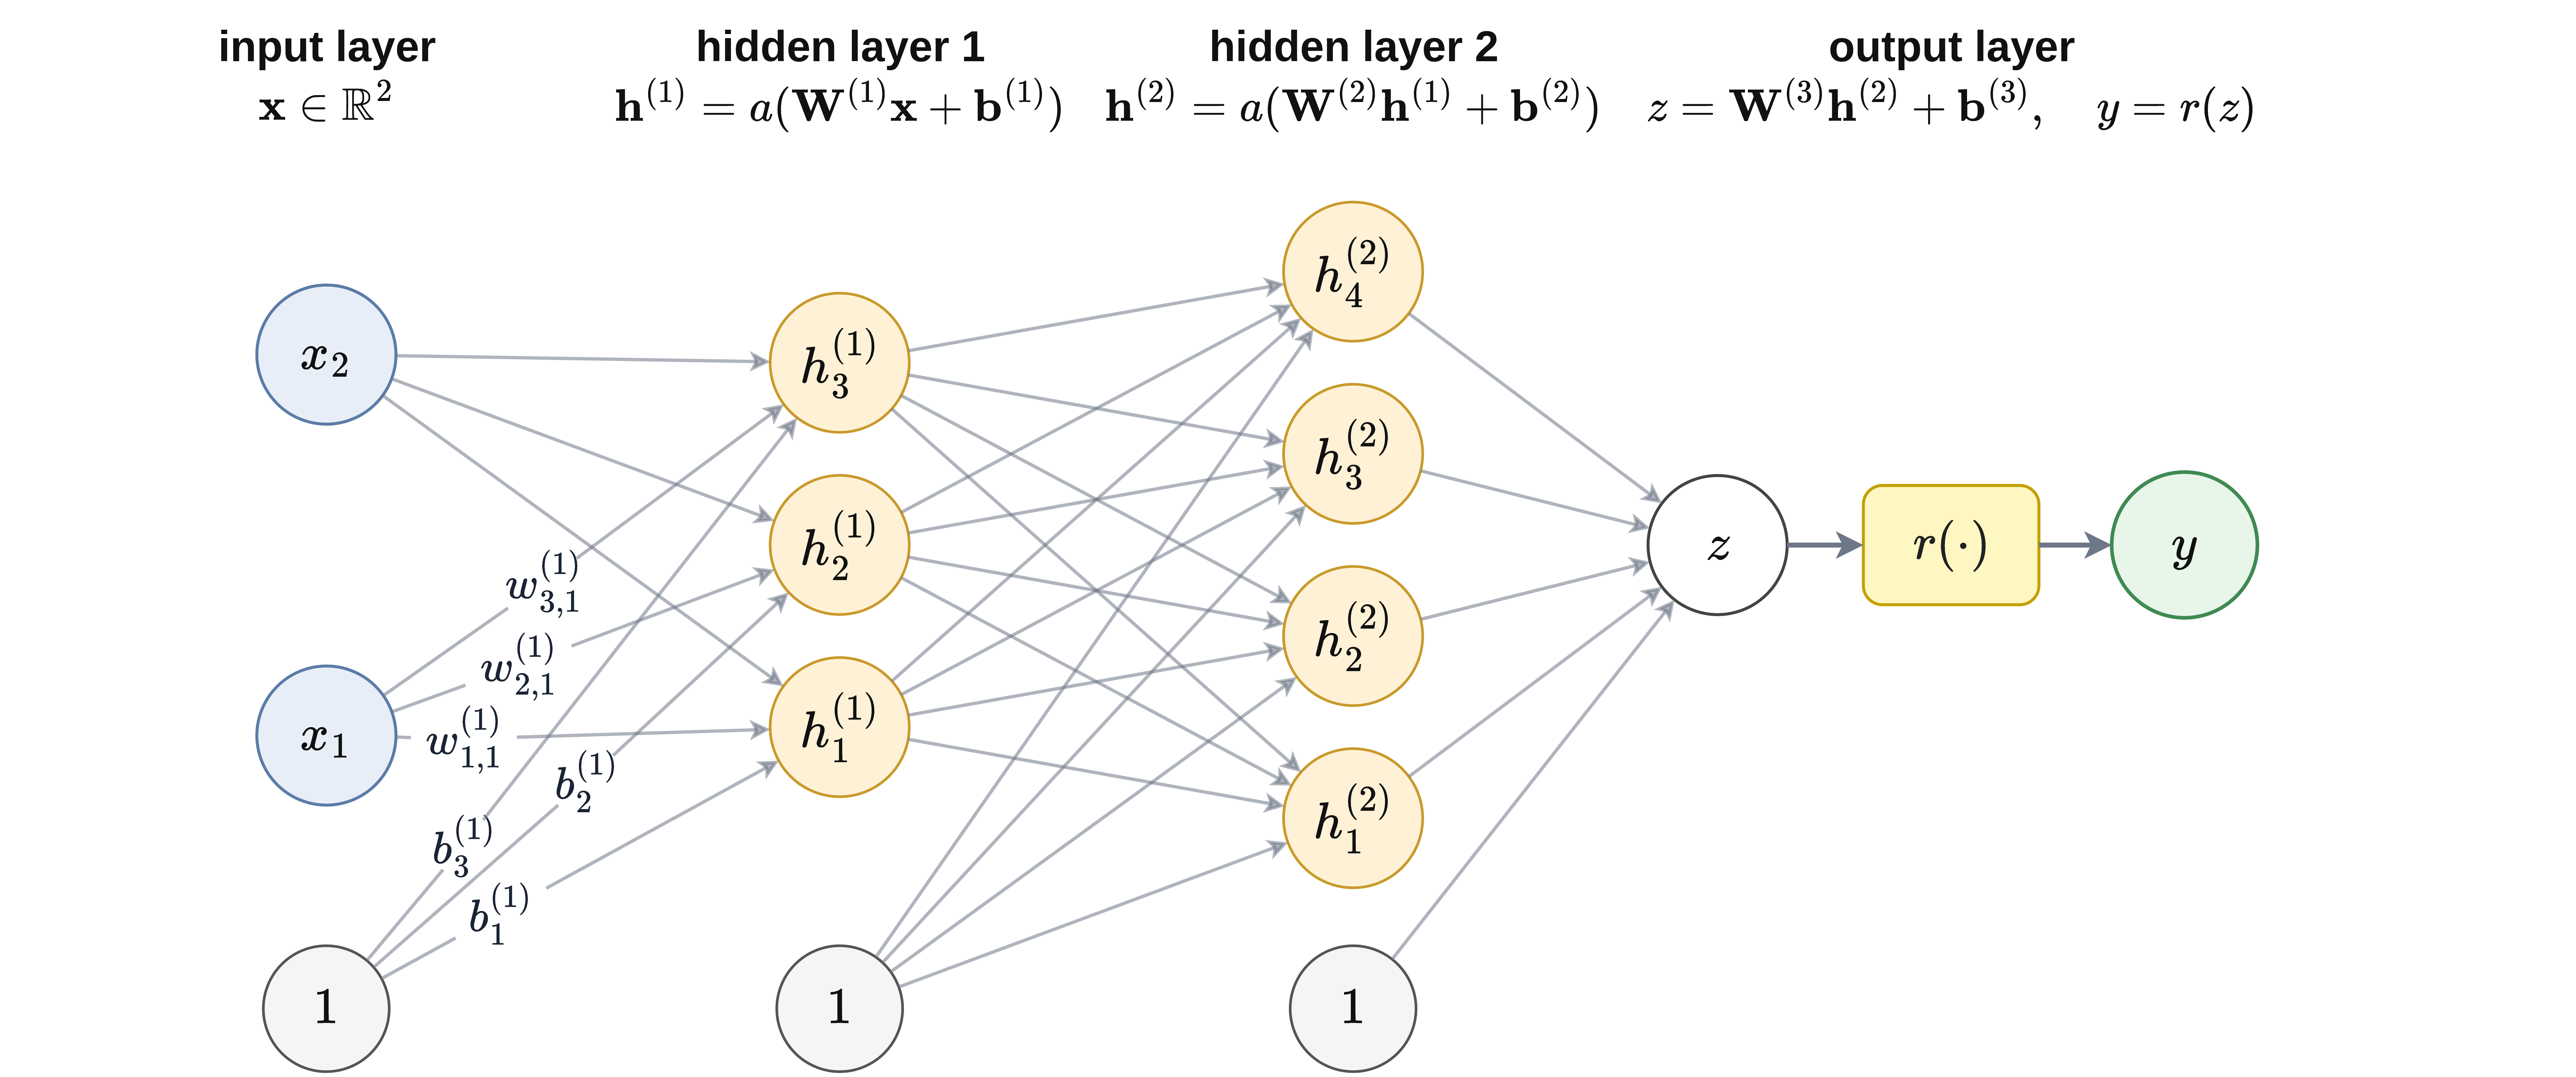
\includegraphics[width=0.7\linewidth,height=\textheight,keepaspectratio]{Figures/neuralnetworks/fig-p3c17-ffnn-architecture.png}

}

\caption{\label{fig-p3c17-ffnn-arch}Schematic of a feed-forward neural
network instantiating (\ref{eq-nnet-forward}) with two inputs
\(x_1, x_2\), two hidden layers of three and four units \(h^{(l)}_j\),
and a scalar output \(y\). Arrows indicate the direction of information
flow; the bias nodes (labeled \(1\)) contribute the additive offsets
\(\mathbf{b}^{(l)}\) in each layer. The edges carrying input \(x_1\) and
the first bias node are labeled with their weights \(w^{(1)}_{j,1}\) and
biases \(b^{(1)}_j\). The output layer is split into the pre-response
value \(z\) and the response function \(r(\,\cdot\,)\) (yellow box)
producing \(y = r(z)\).}

\end{figure}%

\subsection{Activations and response
functions}\label{sec-nnet-activations}

Both activation and response functions are prespecified before training.
Activation and response functions may use the same underlying function;
however, they serve different purposes and are usually chosen
independently of each other. Table~\ref{tbl-activations} lists common
activation and response functions used in practice.

\subsubsection{Activation functions}\label{activation-functions}

A network may use the same activation function for all units, different
activation functions across layers, or even different activation
functions within the same layer, although the latter is uncommon in
practice.\index{neural networks!activation function} The default choice
for hidden layers is the \emph{rectified linear unit} (ReLU) (Nair and
Hinton 2010) due to its computational simplicity and favorable gradient
properties. As ReLU is piecewise linear, a network composed entirely of
ReLU activations represents a piecewise-linear function with finitely
many breakpoints.\index{neural networks!activation function!ReLU} A
network of the same size but only using \(\tanh\) activations would
instead produce smoother curves (see
Figure~\ref{fig-p3c17-mcycle-ffnn}).
\index{neural networks!activation function!tanh@$\tanh$} Smooth
ReLU-like alternatives such as \emph{GELU} (Hendrycks and Gimpel 2016)
and \emph{SiLU/Swish} (Ramachandran, Zoph, and Le 2017) are common in
modern deep learning architectures (Section~\ref{sec-nnet-beyond-ffnn}).
\index{neural networks!activation function!GeLU}\index{neural networks!activation function!SiLU}
GELU is widely used in transformer models, while SiLU is frequently used
in contemporary convolutional neural networks and large language
models.\index{neural networks!convolutional neural network}\index{neural networks!large language model}

\subsubsection{Response functions}\label{response-functions}

The \emph{response function} controls the range of the output and is
usually dictated by the application rather than by computational
considerations.\index{neural networks!response function} In the deep
learning literature, \(r(\,\cdot\,)\) is commonly referred to as the
\emph{output activation} and is treated just like another activation.
The term `response function' is used here to emphasize its different
role.

Common examples of \(r(\,\cdot\,)\) are (Table~\ref{tbl-activations}):

\begin{itemize}
\tightlist
\item
  \emph{identity}, \(r(z) = z\): for deterministic regression when the
  outcome lies in
  \(\mathbb{R}\);\index{neural networks!response function!identity}
\item
  \emph{sigmoid}: to constrain \(r(z) \in (0,1)\) for binary
  classification;\index{neural networks!response function!sigmoid}
\item
  \emph{softmax}, \(r(\mathbf{z})_k = e^{z_k}/\sum_{j=1}^{K}e^{z_j}\):
  to transform an output vector, \(\mathbf{z}\), into a vector of
  non-negative values that sum to one for multi-class classification
  problems;\index{neural networks!response function!softmax}
\item
  \emph{softplus} or \emph{exponential}: common choices to constrain
  \(r(z) \in \mathbb{R}_{>0}\).\index{neural networks!response function!softplus}
\end{itemize}

\begin{longtable}[]{@{}
  >{\raggedright\arraybackslash}p{(\linewidth - 6\tabcolsep) * \real{0.1875}}
  >{\raggedright\arraybackslash}p{(\linewidth - 6\tabcolsep) * \real{0.3750}}
  >{\raggedright\arraybackslash}p{(\linewidth - 6\tabcolsep) * \real{0.2188}}
  >{\centering\arraybackslash}p{(\linewidth - 6\tabcolsep) * \real{0.2188}}@{}}
\caption{Common functions used as activations and response
functions.}\label{tbl-activations}\tabularnewline
\toprule\noalign{}
\begin{minipage}[b]{\linewidth}\raggedright
Name
\end{minipage} & \begin{minipage}[b]{\linewidth}\raggedright
Definition
\end{minipage} & \begin{minipage}[b]{\linewidth}\raggedright
Range
\end{minipage} & \begin{minipage}[b]{\linewidth}\centering
Shape
\end{minipage} \\
\midrule\noalign{}
\endfirsthead
\toprule\noalign{}
\begin{minipage}[b]{\linewidth}\raggedright
Name
\end{minipage} & \begin{minipage}[b]{\linewidth}\raggedright
Definition
\end{minipage} & \begin{minipage}[b]{\linewidth}\raggedright
Range
\end{minipage} & \begin{minipage}[b]{\linewidth}\centering
Shape
\end{minipage} \\
\midrule\noalign{}
\endhead
\bottomrule\noalign{}
\endlastfoot
ReLU & \(a(v) = \max(0, v)\) & \([0, \infty)\) &
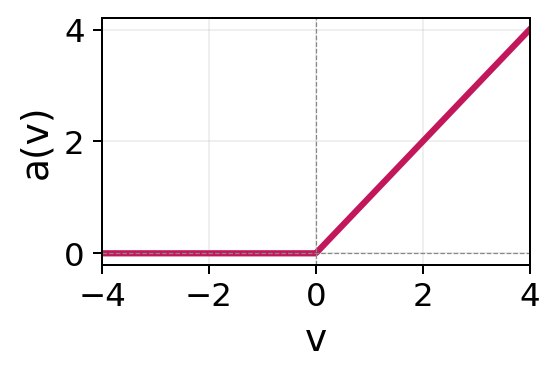
\includegraphics[width=\linewidth,height=0.9375in,keepaspectratio]{Figures/neuralnetworks/fig-p3c17-activation-relu.png} \\
GELU &
\(a(v) = \tfrac{v}{2}\bigl[1 + \operatorname{erf}(v/\sqrt{2})\bigr]\) &
\(\approx [-0.17, \infty)\) &
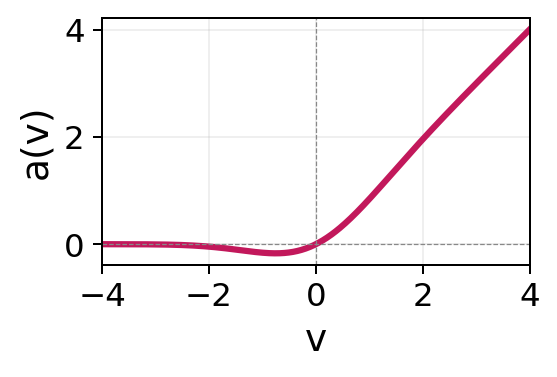
\includegraphics[width=\linewidth,height=0.9375in,keepaspectratio]{Figures/neuralnetworks/fig-p3c17-activation-gelu.png} \\
SiLU & \(a(v) = v / (1 + e^{-v})\) & \(\approx [-0.28, \infty)\) &
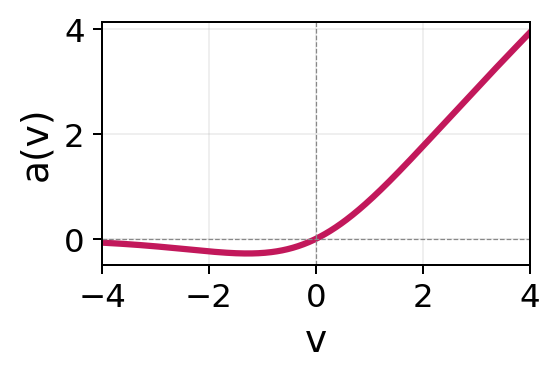
\includegraphics[width=\linewidth,height=0.9375in,keepaspectratio]{Figures/neuralnetworks/fig-p3c17-activation-silu.png} \\
Tanh & \(a(v) = \frac{e^v - e^{-v}}{e^v + e^{-v}}\) & \((-1, 1)\) &
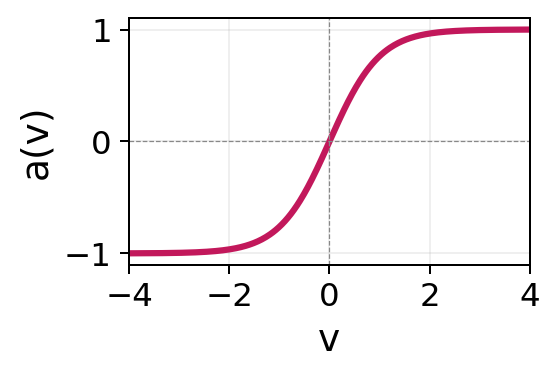
\includegraphics[width=\linewidth,height=0.9375in,keepaspectratio]{Figures/neuralnetworks/fig-p3c17-activation-tanh.png} \\
Sigmoid & \(a(v) = \frac{1}{1 + e^{-v}}\) & \((0, 1)\) &
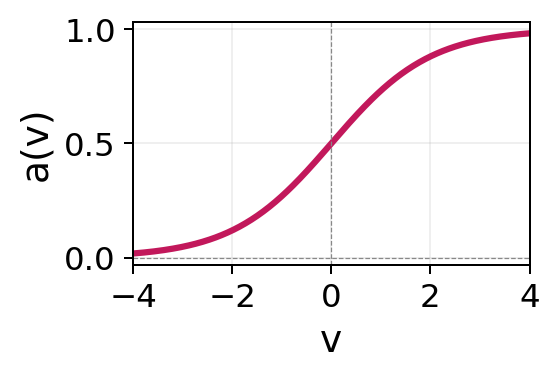
\includegraphics[width=\linewidth,height=0.9375in,keepaspectratio]{Figures/neuralnetworks/fig-p3c17-activation-sigmoid.png} \\
Softplus & \(a(v) = \log(1 + e^v)\) & \((0, \infty)\) &
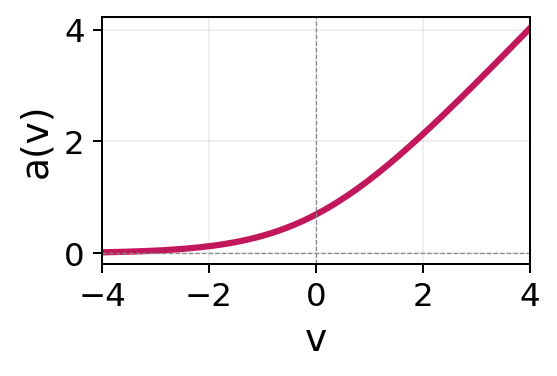
\includegraphics[width=\linewidth,height=0.9375in,keepaspectratio]{Figures/neuralnetworks/fig-p3c17-activation-softplus.png} \\
\end{longtable}

As a running example, the bivariate \texttt{mcycle} dataset (Silverman
1985) records \(n = 133\) measurements of \emph{head acceleration} (in
units of \(g\)) at successive times (measured in milliseconds) following
impact on a helmeted crash-test dummy in a simulated motorcycle crash
(Table~\ref{tbl-mcycle}). The shape of the curve formed by the
observations is non-monotone, with a steep negative spike (deceleration)
at the moment of impact, a positive rebound shortly afterwards, followed
by a relatively stable tail.

\begin{longtable}[]{@{}rr@{}}
\caption{First five rows of the \texttt{mcycle} dataset (Silverman
1985).}\label{tbl-mcycle}\tabularnewline
\toprule\noalign{}
Time (ms) & Acceleration (g) \\
\midrule\noalign{}
\endfirsthead
\toprule\noalign{}
Time (ms) & Acceleration (g) \\
\midrule\noalign{}
\endhead
\bottomrule\noalign{}
\endlastfoot
2.4 & 0.0 \\
2.6 & -1.3 \\
3.2 & -2.7 \\
3.6 & 0.0 \\
4.0 & -2.7 \\
\end{longtable}

Figure~\ref{fig-p3c17-mcycle-ffnn} shows two FFNNs using identical
architectures (same as Figure~\ref{fig-p3c17-ffnn-arch}) and parameters,
with the only difference being the choice of activations. The smooth
curve in the left panel is achieved using \(\tanh\) activations, whereas
the right panel is from a ReLU network, which is clearly visible in the
figure through the small number of sharp corners in the fitted curve
that arise from the piecewise-linear activations. With more hidden
units, the ReLU breakpoints would become dense enough that its fit would
also appear smooth; \(\tanh\) simply achieves a smooth fit with fewer
units.

\begin{figure}

\centering{

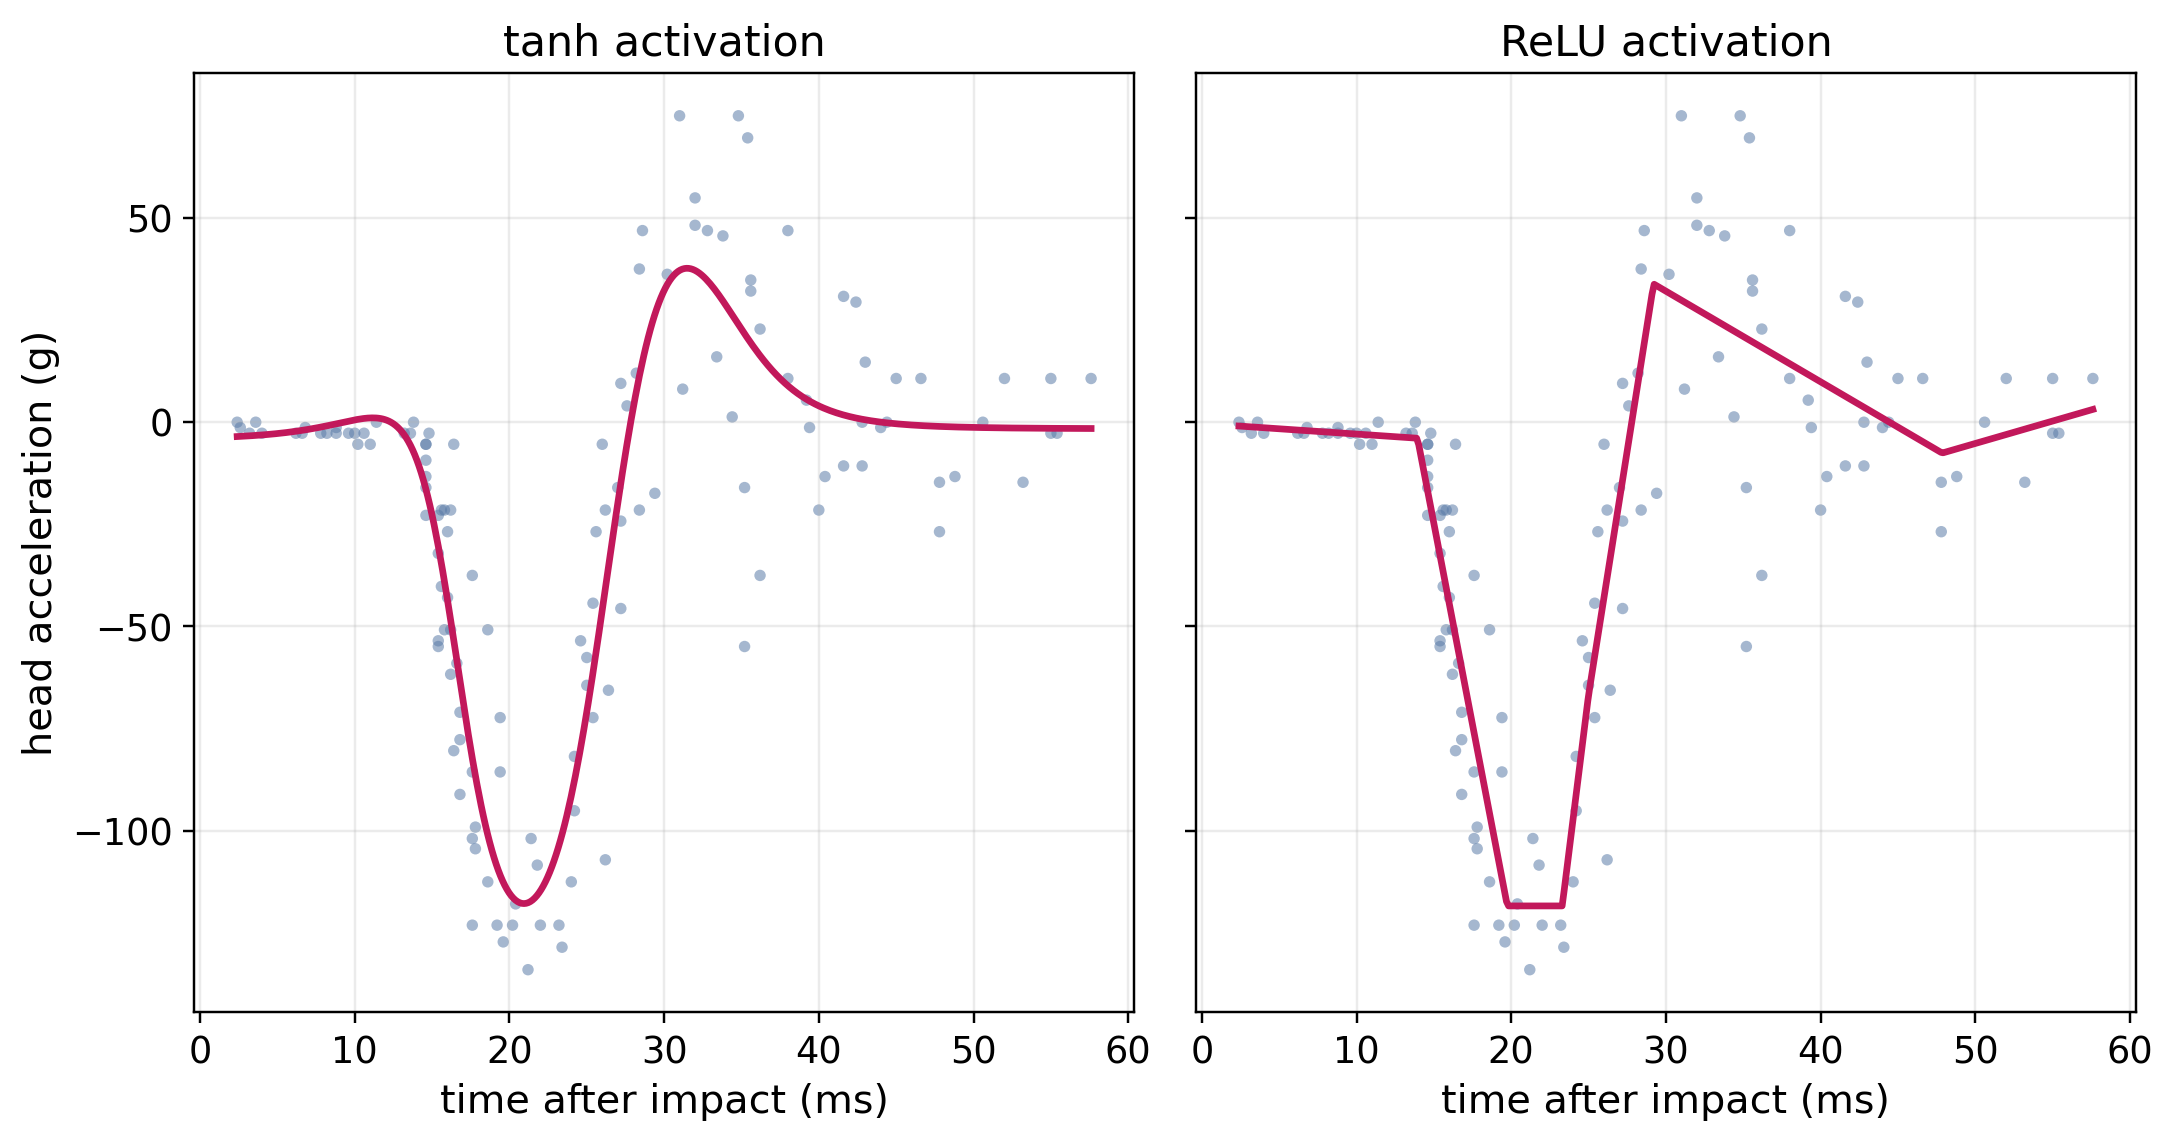
\includegraphics[width=0.9\linewidth,height=\textheight,keepaspectratio]{Figures/neuralnetworks/fig-p3c17-mcycle-tanh-vs-relu.png}

}

\caption{\label{fig-p3c17-mcycle-ffnn}FFNN fits to the \texttt{mcycle}
data. Both panels use the same architecture but with different
activations: \(\tanh\) (left) and ReLU (right).}

\end{figure}%

\subsection{Optimization}\label{sec-nnet-optimization}

As with boosting (Chapter~\ref{sec-boost}), fitting the model in
(\ref{eq-nnet-forward}) to training data involves estimating the
parameters \(\boldsymbol{\theta}\) to minimize a \emph{loss function},
\(L(\boldsymbol{\theta})\), so that:\index{neural networks!optimization}

\begin{equation}\phantomsection\label{eq-nnet-argmin}{
\hat{\boldsymbol{\theta}} \;=\; \mathop{\mathrm{arg\,min}}_{\boldsymbol{\theta}}\, L(\boldsymbol{\theta}).
}\end{equation}

A closed-form minimum to (\ref{eq-nnet-argmin}) does not generally exist
for neural networks and instead \(\hat{\boldsymbol{\theta}}\) has to be
found \emph{iteratively} by gradient descent.
Section~\ref{sec-ml-gradient-descent} introduced the simplest version of
this procedure, referred to here as \emph{plain gradient
descent}.\index{neural networks!gradient descent}

Training a neural network consists of repeatedly performing three
operations for a fixed number of iterations,
\(M\).\index{neural networks!hyperparameters!epochs} As with boosting
(Chapter~\ref{sec-boost}), \(M\) is usually chosen to be large and
training is terminated by early stopping
(Section~\ref{sec-ml-early-stopping}).\index{early stopping} First, the
network passes the inputs through (\ref{eq-nnet-forward}), producing
predictions (forward pass). Second, the discrepancy between the
predictions and the observed outcomes is quantified through a loss
function (Chapter~\ref{sec-rules}), and the corresponding gradients are
computed by backpropagation\index{neural networks!backpropagation}
(backward pass). \emph{Backpropagation} efficiently computes gradients
by applying the chain rule layer by layer, starting from the output and
proceeding back to the input (Rumelhart, Hinton, and Williams 1986).
Finally, the gradients are used by an \emph{optimizer}
(Section~\ref{sec-nn-opt}) to update the parameters. One complete pass
through all the training data is called an \emph{epoch} and may consist
of many iterations due to the use of \emph{mini-batches}
(Section~\ref{sec-nn-batches}).
\index{neural networks!epoch}\index{neural networks!mini-batch} In
practice, modern frameworks compute gradients automatically using
\emph{automatic differentiation}, so specifying the forward pass, choice
of optimizer, and batch size is sufficient to define the entire
optimization procedure.\index{neural networks!automatic differentiation}

\begin{tcolorbox}[enhanced jigsaw, toprule=.15mm, bottomtitle=1mm, opacityback=0, breakable, leftrule=.75mm, title={Algorithm 3 (Full-batch plain gradient descent training of a neural
network)}, toptitle=1mm, bottomrule=.15mm, colback=white, colframe=quarto-callout-note-color-frame, titlerule=0mm, opacitybacktitle=0.6, coltitle=black, rightrule=.15mm, left=2mm, colbacktitle=quarto-callout-note-color!10!white, arc=.35mm]

\textbf{Inputs:} training set
\(\mathcal{D}_{train}= \{(\mathbf{x}_i, y_i)\}_{i=1}^{n}\), loss
\(L(\boldsymbol{\theta}) = \tfrac{1}{n}\sum_{i=1}^{n} \ell_i(\boldsymbol{\theta})\),
learning rate \(\alpha\), number of iterations \(M\), optimizer update
rule \(U\).

\begin{enumerate}
\def\labelenumi{\arabic{enumi}.}
\tightlist
\item
  \(\boldsymbol{\theta}^{0} \gets\) random initialization;
\item
  \textbf{for} \(m = 0, 1, \ldots, M - 1\):
\item
  ~~~~~\textbf{Forward pass:} compute predictions
  \(g(\mathbf{x}_i \mid \boldsymbol{\theta}^{m})\) for
  \(i = 1, \ldots, n\) and loss \(L(\boldsymbol{\theta}^{m})\)
\item
  ~~~~~\textbf{Backward pass:} compute the gradient
  \(\boldsymbol{\gamma}^{m} = \nabla_{\boldsymbol{\theta}} L(\boldsymbol{\theta}^{m})\)
  via backpropagation
\item
  ~~~~~\textbf{Update:}
  \((\boldsymbol{\theta}^{m+1}) \gets U(\boldsymbol{\theta}^{m}, \boldsymbol{\gamma}^{m}, \alpha)\)
\item
  \textbf{end for}
\item
  \textbf{return}
  \(\hat{\boldsymbol{\theta}} \gets \boldsymbol{\theta}^{M}\)
\end{enumerate}

\end{tcolorbox}

Algorithm 3 presents training in its simplest form with plain full-batch
gradient descent. It is common to instead update neural networks using
subsets of the data (the same principle used in random forests and
boosting) and to replace plain gradient descent with an alternative
optimizer. Both ideas are discussed in turn.

\subsubsection{Stochastic gradient descent and
mini-batching}\label{sec-nn-batches}

Using the notation in Algorithm 3, let
\(U(\boldsymbol{\theta}, \boldsymbol{\gamma}, \alpha)\) be an update
rule with parameters \(\boldsymbol{\theta}\), gradients,
\(\boldsymbol{\gamma}\), and learning rate
\(\alpha\).\index{gradient descent} Using plain gradient descent
(described in Section~\ref{sec-ml-gradient-descent}) as the update rule
gives:

\[
U(\boldsymbol{\theta}, \boldsymbol{\gamma}, \alpha) = \boldsymbol{\theta}- \alpha\boldsymbol{\gamma},
\]

which is the identical form to (\ref{eq-ml-gd}).

In Steps 3--4 of Algorithm 3 the \emph{full-batch} gradient,

\[
\nabla_{\boldsymbol{\theta}} L(\boldsymbol{\theta}) \;=\; \frac{1}{n}\sum_{i=1}^{n} \nabla_{\boldsymbol{\theta}}\,\ell_i(\boldsymbol{\theta}),
\]

is evaluated by summing over the entire training set. This requires one
forward and one backward pass through all \(n\) observations for
\emph{each} parameter update. This is prohibitively expensive for the
dataset sizes associated with deep learning. Even when feasible,
full-batch updates are usually suboptimal in practice (as also discussed
in Chapter~\ref{sec-boost}).

Therefore, in each iteration \(m\), neural networks are typically
trained in \emph{mini-batches}, which are small, equally sized, random
subsets of the training data,
\(\mathcal{B}_m \subset \{1, \ldots, n\}\), where each batch is a fixed
size \(B\).\index{neural networks!gradient descent!mini-batch} In
contrast to bootstrapping (Chapter~\ref{sec-ranfor}), mini-batches are
created by shuffling and partitioning the data into approximately
\(\lceil n / B \rceil\) batches, ensuring every observation is used
exactly once per
epoch.\index{neural networks!hyperparameters!mini-batch size}

In steps 3--4 of Algorithm 3, the full-batch loss,
\(L(\boldsymbol{\theta})\), and gradient
\(\nabla_{\boldsymbol{\theta}} L(\boldsymbol{\theta}^{m})\), are
replaced by a \emph{mini-batch loss} and gradient,

\begin{equation}\phantomsection\label{eq-nnet-minibatch}{
L_{\mathcal{B}_m}(\boldsymbol{\theta}) \;=\; \frac{1}{B}\sum_{i \in \mathcal{B}_m} \ell_i(\boldsymbol{\theta}),
\qquad
\nabla_{\boldsymbol{\theta}} L_{\mathcal{B}_m}(\boldsymbol{\theta}^{m}) \;=\; \frac{1}{B}\sum_{i \in \mathcal{B}_m}\nabla_{\boldsymbol{\theta}}\,\ell_i(\boldsymbol{\theta}^{m}).
}\end{equation}

As well as being more computationally efficient, the stochasticity
introduced by `mini-batching' can help the optimization escape narrow
saddle points and shallow local minima, often leading to improved
generalization.

The resulting procedure is called (mini-batch) \emph{stochastic gradient
descent} (SGD) (Robbins and Monro 1951). Conceptually, training can be
viewed as two nested loops: an inner loop consisting of steps 3--5,
repeated once per mini-batch, and an outer loop of steps 2--6, repeated
once per epoch, where an \emph{epoch} is a complete pass through the
training data.\index{neural networks!epoch} The term \emph{iteration} is
avoided from this point as its meaning depends on which loop is being
referenced.

\subsubsection{Optimizers}\label{sec-nn-opt}

Plain gradient descent (including its stochastic and mini-batch
variants) is the simplest choice for the optimizer,
\(U\).\index{neural networks!optimizer} It applies the same learning
rate, \(\alpha\), to every parameter and uses no information from past
gradients.\index{neural networks!hyperparameters!learning rate} Modern
\emph{adaptive} optimizers improve on plain gradient descent by
maintaining a running estimate of the gradient direction
(\emph{momentum}) and the per-parameter gradient magnitude
(\emph{scaling}). These quantities are used to adapt the effective step
size during training.\index{neural networks!optimizer!adaptive}

The quantities required by an optimizer are stored in an internal state,
\(\mathbf{s}\), which contains any additional information needed to
compute the parameter updates. The optimizer in Algorithm 3 can then be
written as
\(U(\boldsymbol{\theta}, \boldsymbol{\gamma}, \alpha, \mathbf{s})\) and
the first step of the algorithm would set an initial state,
\(\mathbf{s}^0\). For plain gradient descent, the state is empty,
\(\mathbf{s}= ()\).\index{neural networks!optimizer!state}

The most widely used optimizer in deep learning is \emph{Adam} (Adaptive
Moment Estimation) (Kingma and Ba 2015). Adam maintains exponential
moving averages of the gradient and the element-wise squared gradient,
\index{neural networks!optimizer!Adam}

\begin{equation}\phantomsection\label{eq-nnet-adam-moments}{
\begin{aligned}
\bar{\boldsymbol{\gamma}}^{m} &= \nu_1\,\bar{\boldsymbol{\gamma}}^{m-1} + (1 - \nu_1)\,\boldsymbol{\gamma}^{m},\\
\mathbf{v}^{m} &= \nu_2\,\mathbf{v}^{m-1} + (1 - \nu_2)\,(\boldsymbol{\gamma}^{m})^2,
\end{aligned}
}\end{equation}

where \(\boldsymbol{\gamma}^{m}\) is the gradient supplied to \(U\) in
Step 5 of Algorithm 3. The quantities \(\bar{\boldsymbol{\gamma}}^{m}\)
and \(\mathbf{v}^{m}\) are exponential moving averages of the gradient
and element-wise squared gradient, respectively, and
\(\nu_1, \nu_2 \in [0, 1)\) are the corresponding decay rates. After a
bias correction that compensates for the zero-initialization of
\(\bar{\boldsymbol{\gamma}}\) and \(\mathbf{v}\) (omitted here for
brevity), the parameter update is:

\begin{equation}\phantomsection\label{eq-nnet-adam-update}{
\boldsymbol{\theta}^{m+1} \;=\; \boldsymbol{\theta}^{m} - \alpha\,\frac{\bar{\boldsymbol{\gamma}}^{m}}{\sqrt{\mathbf{v}^{m}} + \epsilon},
}\end{equation}

where \(\epsilon > 0\) is a small numerical-stability constant
(typically \(10^{-8}\)) that prevents division by zero whenever a
component \(v_j^{m}\) of \(\mathbf{v}^{m}\) is close to zero. The state,
\(\mathbf{s}^m = (\bar{\boldsymbol{\gamma}}^m, \mathbf{v}^m)\), is
updated according to (\ref{eq-nnet-adam-moments}) and the resulting
values are used to update \(\boldsymbol{\theta}\) via
(\ref{eq-nnet-adam-update}).

The numerator, \(\bar{\boldsymbol{\gamma}}^{m}\), is the momentum term,
which here averages recent gradients and thereby reduces noise from
mini-batching while accelerating descent along persistent directions.
The denominator, \(\sqrt{\mathbf{v}^{m}}\), is the scaling term, which
rescales each coordinate by its own recent gradient magnitude, so
parameters whose gradients are large get \emph{smaller} steps and
parameters whose gradients are small get \emph{larger} steps. These
features make Adam much less sensitive to the choice of \(\alpha\) than
plain SGD and substantially reduce the need to tune separate learning
rates.

\subsection{Managing hyperparameters}\label{sec-nnet-hyperparameters}

One feature of neural networks that can be considered both a strength
and a drawback is the number of hyperparameters
(Section~\ref{sec-ml-models}) that must be configured. In the context of
neural networks, hyperparameters can be grouped into two categories.

\subsubsection{Structural
hyperparameters}\label{structural-hyperparameters}

\emph{Structural hyperparameters} define the structure of the neural
network.\index{neural networks!hyperparameters!structural} They include
the choice of architecture family (Section~\ref{sec-nnet-beyond-ffnn}),
the \emph{depth} (number of hidden layers, \(L\)) and \emph{width}
(number of units per layer) of the network, the choice of hidden
activations, \(a^{(l)}\), and the response function,
\(r\).\index{neural networks!hyperparameters!depth}\index{neural networks!hyperparameters!width}
Together, these choices determine the class of functions that the
network can represent, and therefore the solutions available to gradient
descent.

Attempting to tune these hyperparameters is computationally expensive as
each candidate configuration requires a full training run, which could
take hours or even days. \emph{Neural architecture search} (NAS)
(Elsken, Metzen, and Hutter 2019) automates the search using
reinforcement learning, evolutionary algorithms, or gradient-based
relaxations of the discrete
choices.\index{neural networks!neural architecture search} However, NAS
is itself extremely compute-intensive and largely confined to settings
where the same architecture will be reused many times (for example in
image classification).

For most applications the architecture is therefore \emph{chosen}, not
tuned, drawing on the families of Section~\ref{sec-nnet-beyond-ffnn} and
on what is standard in the relevant domain. A complementary strategy is
to deliberately over-parameterize the network, that is, to use more
layers or units than are strictly necessary so that the network is
sufficiently flexible to model complex
relationships.\index{over-parameterization} Overfitting is then
controlled through regularization rather than by carefully tuning the
network
capacity.\index{regularization}\index{neural networks!regularization}
Two \emph{regularization} strategies are particularly common to help
reduce overfitting:

\begin{itemize}
\tightlist
\item
  \emph{Weight decay} adds a shrinkage penalty
  \(\lambda\|\boldsymbol{\theta}\|_2^2\) to the loss for some
  \(\lambda \in \mathbb{R}_{>0}\), identical to the ridge penalty in the
  linear case.\index{neural networks!regularization!weight decay}
\item
  \emph{Dropout} (Srivastava et al. 2014) randomly sets a fraction,
  \(p\), of activations to zero during each training step, which can be
  interpreted as implicit ensembling over thinned
  sub-networks.\index{neural networks!regularization!dropout proportion}
\end{itemize}

\(\lambda\) and \(p\) are mathematical hyperparameters, but they are
typically robust and may be tuned over a small discrete grid of
candidate
values.\index{neural networks!hyperparameters!shrinkage penalty}\index{neural networks!hyperparameters!dropout proportion}
Over-parameterization alongside weight decay and/or dropout is therefore
a common method to reduce the need to tune structural hyperparameters,
at the cost of only one or two extra hyperparameters.

Beyond these explicit regularization methods, training an
over-parameterized network with (stochastic) gradient descent includes
its own \emph{implicit regularization}. Large networks may have many
parameter settings that fit the training data equally well, but gradient
descent usually favors solutions that are comparatively simple and
generalize well to unseen data.

\subsubsection{Mathematical
hyperparameters}\label{mathematical-hyperparameters}

\emph{Mathematical hyperparameters} control \emph{how} the parameters
are estimated once the network structure has been
fixed.\index{neural networks!hyperparameters!mathematical} They include
the learning rate
\(\alpha\),\index{neural networks!hyperparameters!learning rate}
optimizer hyperparameters (such as Adam's decay rates from
(\ref{eq-nnet-adam-moments})),\index{neural networks!hyperparameters!decay rate}
the mini-batch size,
\(B\),\index{neural networks!hyperparameters!mini-batch size} from
(\ref{eq-nnet-minibatch}), the number of training
epochs\index{neural networks!hyperparameters!epochs}, \(M\),
early-stopping settings, and the regularization hyperparameters
discussed above.

Adaptive optimizers, such as Adam, are relatively insensitive to the
choice of learning rate. It is therefore common to set a small learning
rate (such as \(0.001\) (Allaire and Chollet 2020)) rather than
performing extensive tuning.\index{neural networks!optimizer!Adam} As
with gradient boosting machines, the number of epochs is also usually
not tuned but instead a sufficiently large number is chosen and then
early stopping (Section~\ref{sec-ml-early-stopping}) is used to
terminate training once a held-out validation loss stops
improving.\index{gradient boosting machines} The remaining mathematical
hyperparameters can then be tuned using nested cross-validation
(Section~\ref{sec-ml-opt}).
\index{resampling!cross-validation}\index{hyperparameter optimization}

\subsection{Probabilistic
predictions}\label{sec-nnet-deterministic-vs-probabilistic}

Recall from Section~\ref{sec-ml-tasks-regr} that regression tasks can be
\emph{deterministic},\index{regression!deterministic} returning a single
point prediction
\(\hat{y}_i = g(\mathbf{x}_i \mid \hat{\boldsymbol{\theta}})\) of the
conditional mean, or
\emph{probabilistic},\index{regression!probabilistic} returning a full
conditional distribution
\(\hat{f}(y \mid \mathbf{x}_i, \hat{\boldsymbol{\theta}})\) from which
means, quantiles, prediction intervals, and predictive densities can be
derived. This distinction is central when adapting neural networks to
survival analysis (Section~\ref{sec-nnet-surv}), where the prediction
targets are inherently distributional (Chapter~\ref{sec-survtsk}).

The fits in Figure~\ref{fig-p3c17-mcycle-ffnn} are deterministic with a
single scalar output: for each observation (time in milliseconds), a
single output is predicted (head acceleration). In that example, the
parameters \(\hat{\boldsymbol{\theta}}\) were obtained by minimizing the
\emph{mean squared error} (MSE), \index{mean squared error}

\begin{equation}\phantomsection\label{eq-nnet-mse}{
\hat{\boldsymbol{\theta}} \;=\; \mathop{\mathrm{arg\,min}}_{\boldsymbol{\theta}}\; \frac{1}{n}\sum_{i=1}^{n}\bigl(y_i - g(\mathbf{x}_i \mid \boldsymbol{\theta})\bigr)^{2},
}\end{equation}

which yields a fitted curve
\(g(\mathbf{x}\mid \hat{\boldsymbol{\theta}})\) that summarizes the
conditional mean.

To instead estimate the full probability distribution, the network must
output all the parameters of an assumed conditional distribution. Any
parametric family \(f(y \mid \boldsymbol{\phi})\) with a differentiable
log-density can be used, where \(\boldsymbol{\phi}\) denotes the vector
of distribution parameters. The network predicts
\(\boldsymbol{\phi}(\mathbf{x}_i) = g(\mathbf{x}_i \mid \boldsymbol{\theta})\),
requiring one output head and corresponding response function for each
component of \(\boldsymbol{\phi}\). The loss used for training is
typically the \emph{negative log-likelihood},
\index{negative log-likelihood}

\begin{equation}\phantomsection\label{eq-nnet-nll}{
-\sum_i \log f(y_i \mid \boldsymbol{\phi}(\mathbf{x}_i)).
}\end{equation}

For this example, consider the normal distribution which predicts the
conditional mean \(\mu(\mathbf{x}\mid \boldsymbol{\theta})\) and the
conditional scale \(\sigma(\mathbf{x}\mid \boldsymbol{\theta})\)
jointly:

\[
g(\mathbf{x}_i \mid \boldsymbol{\theta}) = \bigl(\mu(\mathbf{x}_i \mid \boldsymbol{\theta}),\; \sigma(\mathbf{x}_i \mid \boldsymbol{\theta})\bigr)^\top\in \mathbb{R}\times \mathbb{R}_{>0}.
\]

Positivity of the scale is enforced internally by an exponential
response function (Section~\ref{sec-nnet-activations}) on the
\(\sigma\)-output, \(\sigma = \exp(z_\sigma)\), while the mean uses the
identity response. The training objective is the normal negative
log-likelihood (\ref{eq-nnet-nll}),

\begin{equation}\phantomsection\label{eq-nnet-gauss-nll}{
\begin{aligned}
\hat{\boldsymbol{\theta}}
&= \mathop{\mathrm{arg\,min}}_{\boldsymbol{\theta}}\; -\sum_{i=1}^n \log f(y_i \mid \boldsymbol{\phi}(\mathbf{x}_i)) \\
&= \mathop{\mathrm{arg\,min}}_{\boldsymbol{\theta}}\; \sum_{i=1}^{n} \left[\tfrac{1}{2\,\sigma(\mathbf{x}_i \mid \boldsymbol{\theta})^2}\bigl(y_i - \mu(\mathbf{x}_i \mid \boldsymbol{\theta})\bigr)^2 + \log \sigma(\mathbf{x}_i \mid \boldsymbol{\theta}) + \tfrac{1}{2}\log(2\pi)\right],
\end{aligned}
}\end{equation}

where \(f\) is the normal density with mean
\(\mu(\mathbf{x}_i \mid \boldsymbol{\theta})\) and standard deviation
\(\sigma(\mathbf{x}_i \mid \boldsymbol{\theta})\). The parameters
\(\boldsymbol{\theta}\) now parametrize a whole conditional density
\(f(y \mid \mathbf{x}, \boldsymbol{\theta})\) rather than a single
conditional mean, so the prediction at a new \(\mathbf{x}_*\) is the
full distribution
\(f(\,\cdot \mid \mathbf{x}_*, \hat{\boldsymbol{\theta}})\), from which
means, quantiles, and prediction intervals can be extracted.

Figure~\ref{fig-p3c17-ffnn-distributional} illustrates three ways a
network can produce the two outputs \(\mu(\mathbf{x})\) and
\(\sigma(\mathbf{x})\) that parametrize (\ref{eq-nnet-gauss-nll}). The
part of the network specific to a particular output is called an
\emph{output head}.\index{neural networks!output head} In
Figure~\ref{fig-p3c17-ffnn-distributional} (a), the hidden layers are
fully shared and each output head consists only of a final linear layer
and response function. This is the most parameter-efficient approach, as
the same hidden representation is learned once and reused for both
parameters. In Figure~\ref{fig-p3c17-ffnn-distributional} (b), the
outputs still share an initial representation but each head contains
additional hidden layers, allowing some parameter-specific
specialization. Finally, in Figure~\ref{fig-p3c17-ffnn-distributional}
(c), separate networks predict \(\mu(\mathbf{x})\) and
\(\sigma(\mathbf{x})\) but are still trained jointly through the same
distributional loss. This is the most flexible approach, particularly
when the parameters require different representations or regularization,
but it also has the largest number of parameters.

\begin{figure}

\centering{

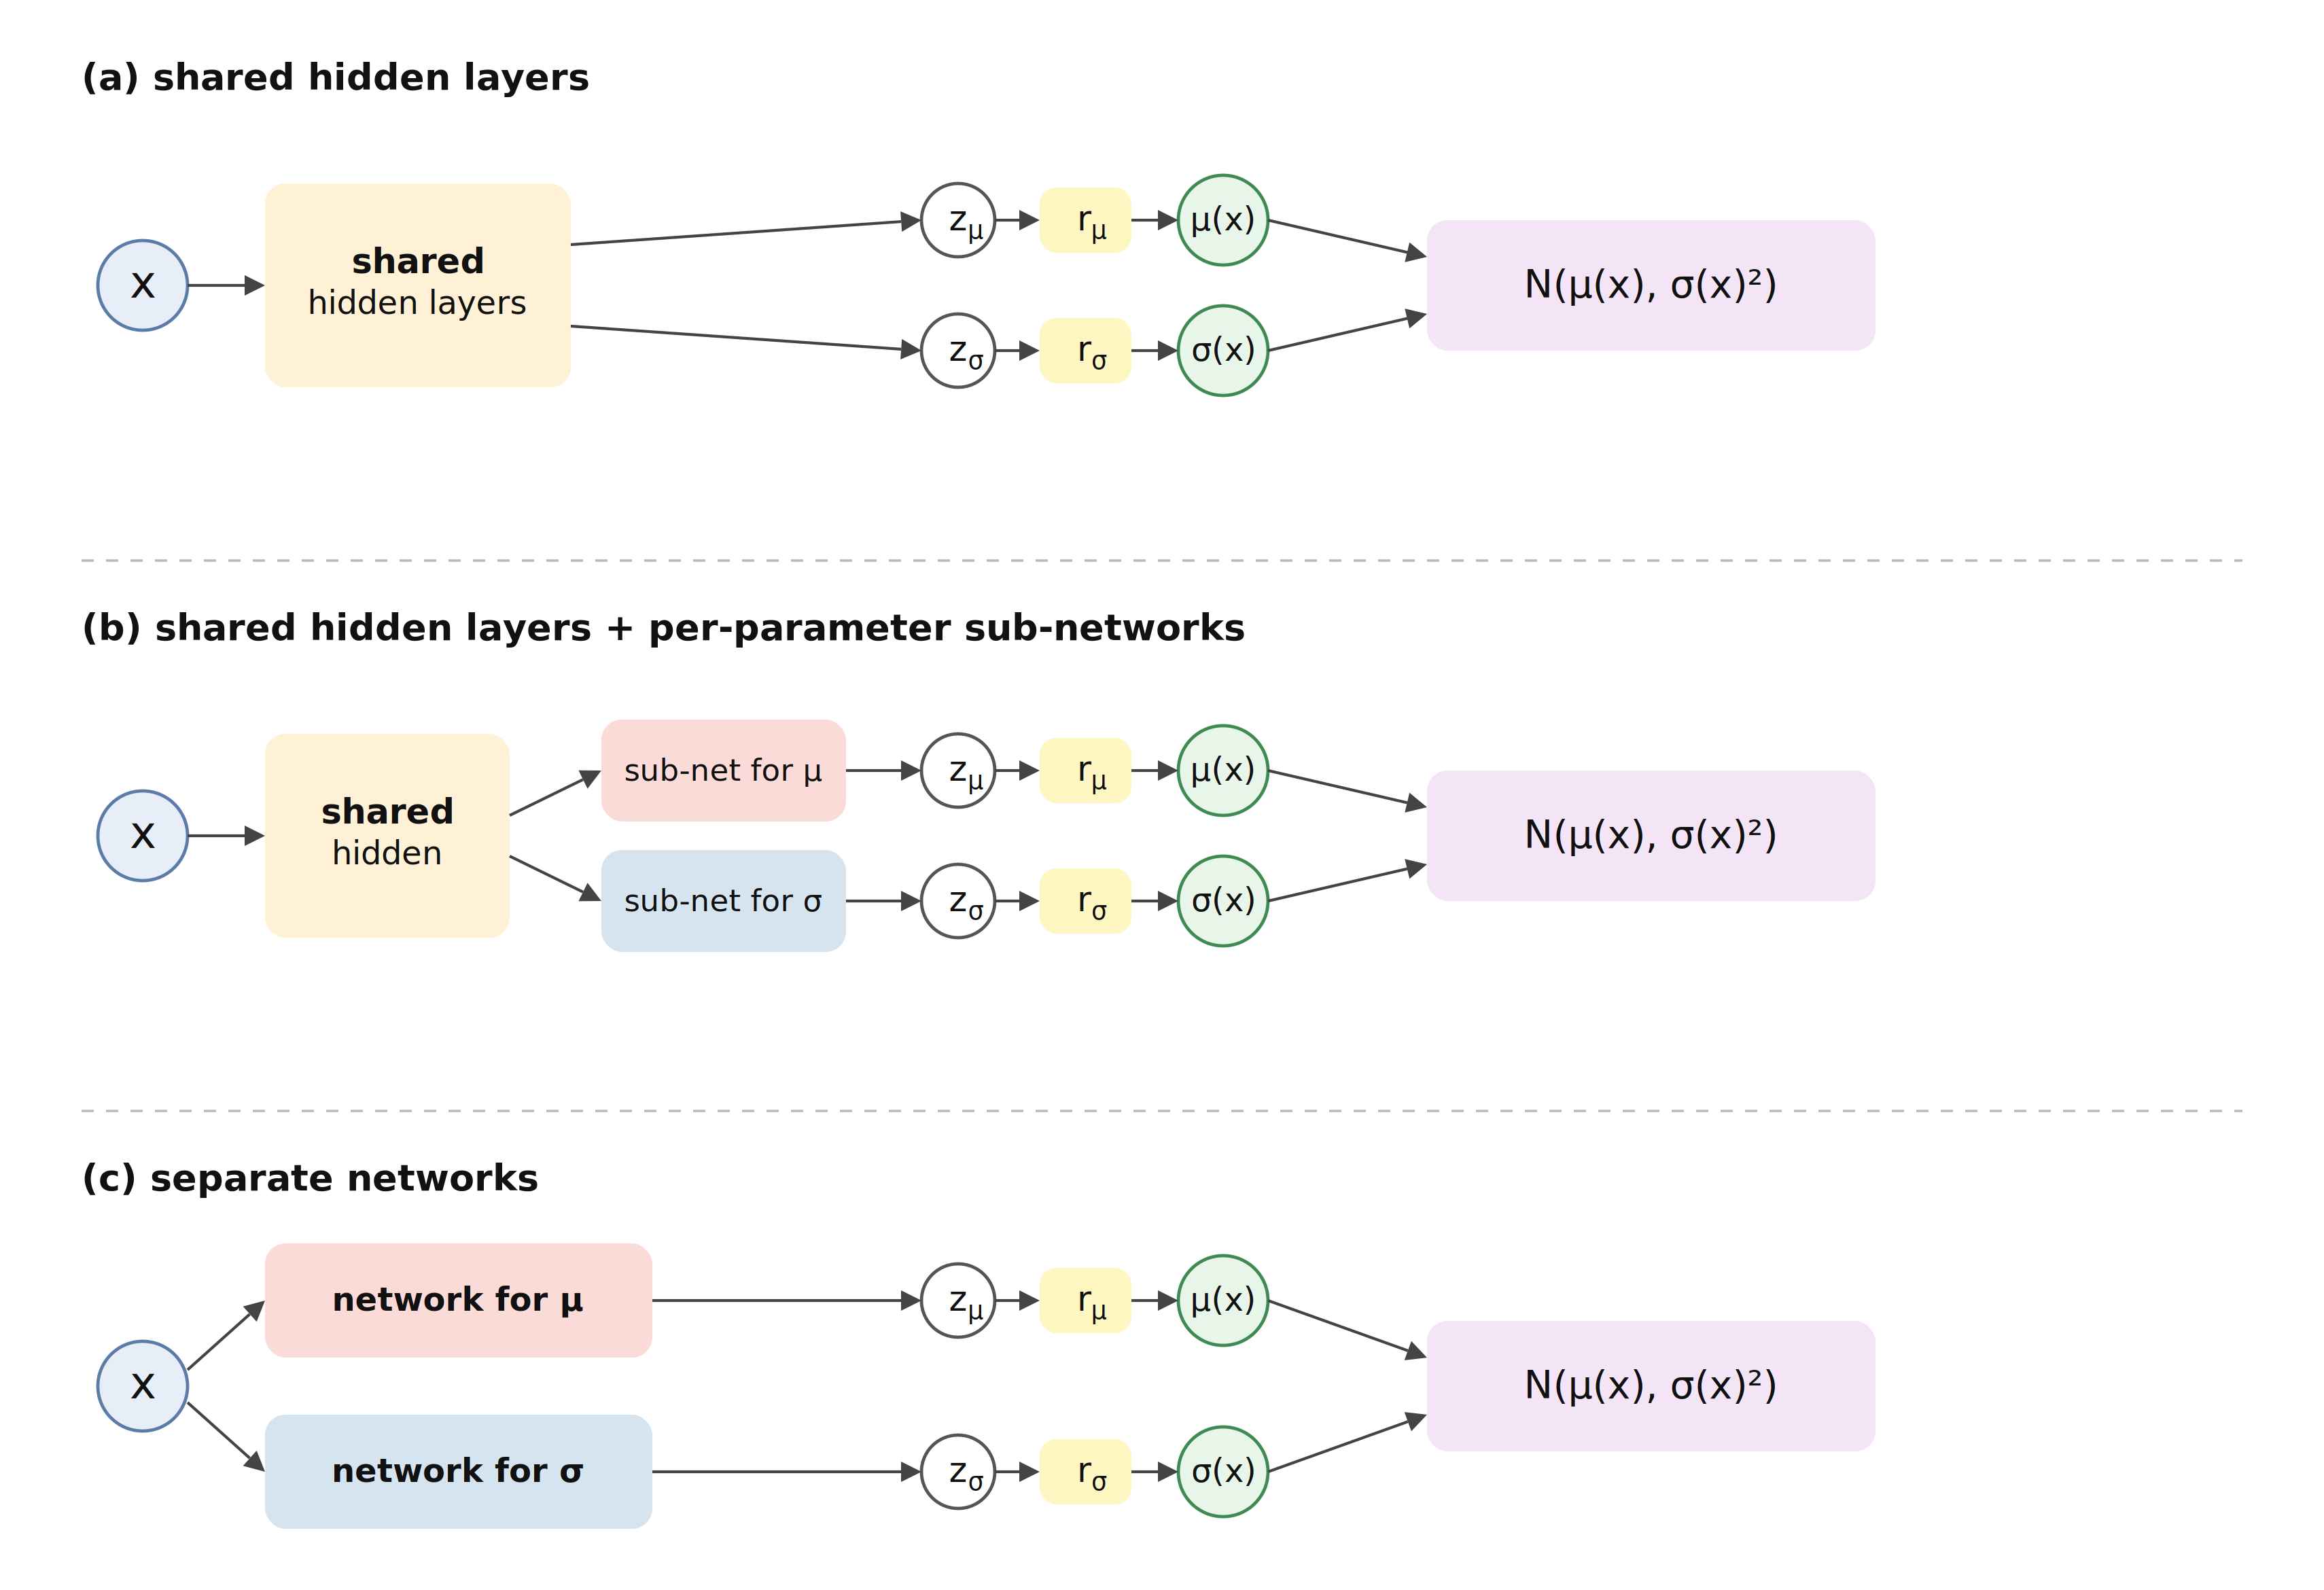
\includegraphics[width=0.85\linewidth,height=\textheight,keepaspectratio]{Figures/neuralnetworks/fig-p3c17-ffnn-distributional.png}

}

\caption{\label{fig-p3c17-ffnn-distributional}Three architectural
variants for probabilistic regression. Top, a): Shared hidden layers
whose final layer splits into two pre-response values
\(z_\mu, z_\sigma\), each mapped through its own response function to
produce \(\mu(\mathbf{x})\) and \(\sigma(\mathbf{x})\). Middle, b):
Shared hidden layers followed by two small per-parameter sub-networks
before each \(z\). Bottom, c): Two entirely separate networks for
\(\mu\) and \(\sigma\). In all three variants the two outputs feed into
the same conditional distribution
\(\mathcal{N}(\mu(\mathbf{x}), \sigma(\mathbf{x})^2)\), so the network
is trained jointly under one distributional loss.}

\end{figure}%

Figure~\ref{fig-p3c17-mcycle-det-vs-prob} visualizes the contrast
between deterministic and probabilistic regression on the
\texttt{mcycle} data.\index{regression!probabilistic} Both panels share
the \emph{same} FFNN architecture (Figure~\ref{fig-p3c17-ffnn-arch});
only the output head and the loss
differ.\index{neural networks!feed-forward neural network} The left
panel is a single-output FFNN trained with the MSE (\ref{eq-nnet-mse});
the prediction is a single curve and does not quantify predictive
uncertainty. The right panel uses fully shared hidden layers
(Figure~\ref{fig-p3c17-ffnn-distributional} (a)) with two output heads,
identity response for \(\mu(\mathbf{x})\) and exponential response for
\(\sigma(\mathbf{x})\), trained with the normal negative log-likelihood
(\ref{eq-nnet-gauss-nll}). Estimation of \(\sigma(\mathbf{x})\) allows
uncertainty to be captured at each time point after impact.

\begin{figure}

\centering{

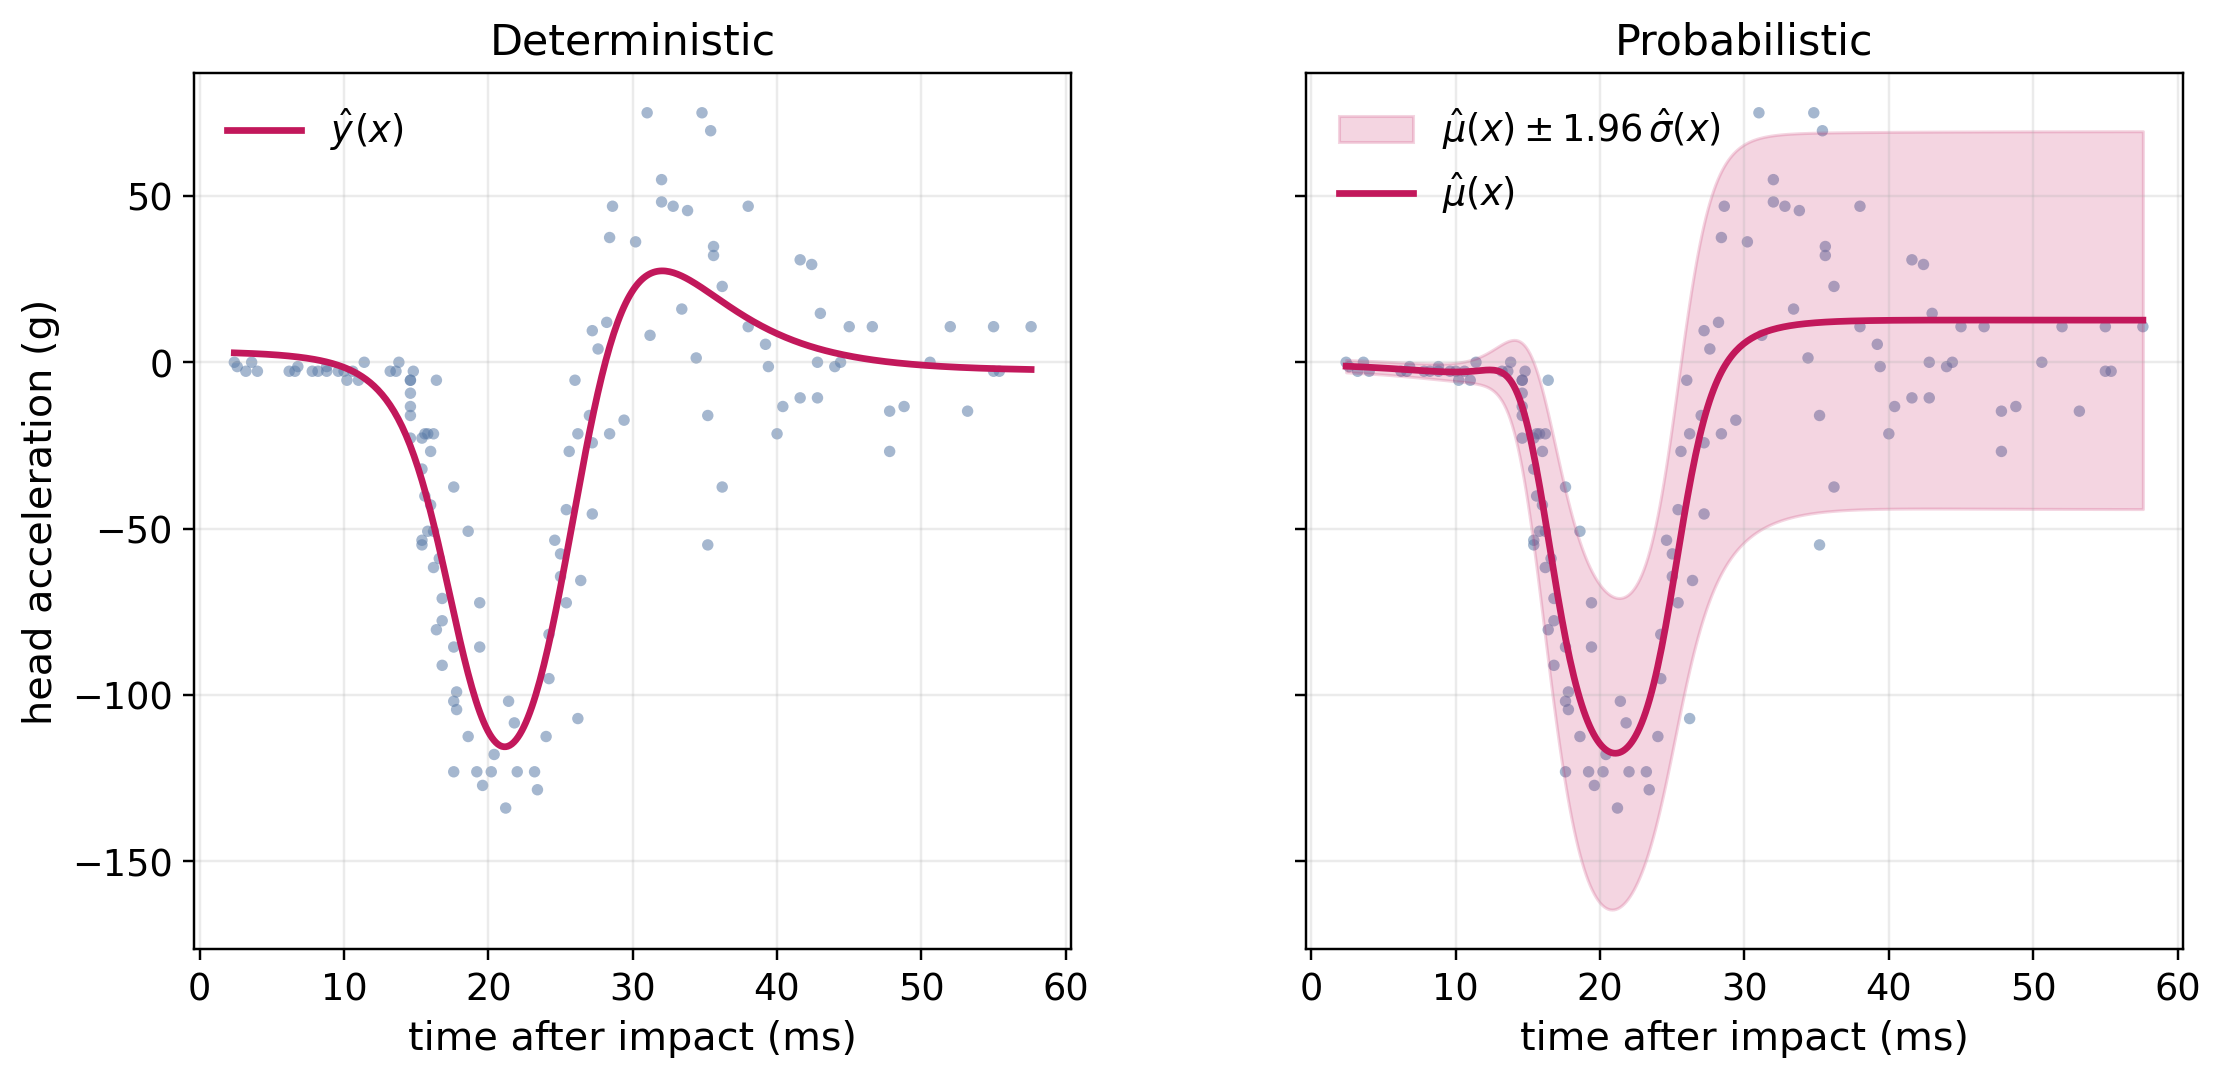
\includegraphics[width=1\linewidth,height=\textheight,keepaspectratio]{Figures/neuralnetworks/fig-p3c17-mcycle-det-vs-prob.png}

}

\caption{\label{fig-p3c17-mcycle-det-vs-prob}Deterministic
vs.~probabilistic regression on the \texttt{mcycle} data using the FFNN
reference architecture of Figure~\ref{fig-p3c17-ffnn-arch} in both
panels. \emph{Left}: a single-output FFNN trained with the MSE of
(\ref{eq-nnet-mse}); the prediction is a single conditional-mean curve
\(\hat{y}(x)\). \emph{Right}: variant \emph{(a)} of
Figure~\ref{fig-p3c17-ffnn-distributional} trained with the normal
negative log-likelihood of (\ref{eq-nnet-gauss-nll}); the prediction is
a whole conditional normal \(\mathcal{N}(\mu(x), \sigma(x)^2)\), shown
as the mean \(\mu(x)\) together with the pointwise central 95\% interval
\(\mu(x) \pm 1.96\,\sigma(x)\) of the predicted outcome distribution.}

\end{figure}%

\subsection{Beyond feed-forward networks}\label{sec-nnet-beyond-ffnn}

The recursion in (\ref{eq-nnet-forward}) defines a fully-connected
feed-forward network, but the optimization procedure of Algorithm 3
applies equally to any composition of differentiable units. Contemporary
architectures share the FFNN's gradient-based optimization and
end-to-end training but differ in the types of patterns they are
designed to capture from the data. The most common families are listed
below with references for further reading.

\begin{itemize}
\tightlist
\item
  \textbf{Convolutional Neural Networks (CNNs)} (Krizhevsky, Sutskever,
  and Hinton 2012; LeCun et al. 1998) exploit local structure in the
  input by analyzing small regions at a time and reusing the same set of
  parameters across all regions. CNNs are the default choice for
  image-like inputs, such as natural images (object detection), medical
  images (histopathology slides), audio spectrograms, and any other
  grid-like data. In survival applications they are commonly used for
  radiology-based time-to-event
  prediction.\index{neural networks!convolutional neural network}
\item
  \textbf{Recurrent Neural Networks (RNNs)}, in particular the
  \emph{long short-term memory} (LSTM) (Hochreiter and Schmidhuber 1997)
  and \emph{gated recurrent unit} (GRU) (Cho et al. 2014), process
  variable-length sequences by maintaining an internal state that
  summarizes previously observed inputs. They are well suited to
  longitudinal data with irregular sampling, including electronic
  health-record event streams and biomarker trajectories, and were the
  dominant choice for sequence modeling until transformers overtook
  them.\index{neural networks!recurrent neural network}
\item
  \textbf{Transformers} (Vaswani et al. 2017) also process sequences but
  replace recurrence with \emph{self-attention}, allowing each input
  element to directly incorporate information from every other element.
  Transformers dominate contemporary natural-language processing (BERT,
  GPT and successors), have largely replaced CNNs at the top of
  large-scale vision benchmarks, and are increasingly used for tabular
  electronic-health-record sequences and multimodal medical data. They
  are computationally heavier than RNNs but capture relationships
  between distant parts of a sequence more
  reliably.\index{neural networks!transformer}\index{neural networks!large language model}\index{multimodal data}
\item
  \textbf{Graph Neural Networks (GNNs)} (L. Wu et al. 2022) generalize
  the idea of convolution to graph-structured data (nodes connected by
  edges) by aggregating information from neighboring nodes (the
  \emph{message-passing} paradigm). They are used wherever the natural
  structure of the data is a graph, for example in molecular property
  prediction for drug discovery, social networks, or recommendation
  systems.\index{neural networks!graph neural network}
\item
  \textbf{Autoencoders} (Hinton and Salakhutdinov 2006) and their
  probabilistic counterparts, \emph{variational autoencoders} (VAEs)
  (Kingma and Welling 2014), learn a compact representation of the data
  by attempting to reconstruct the input after compressing it. They are
  widely used for unsupervised representation learning, dimensionality
  reduction, anomaly detection, and generative modeling of
  high-dimensional data such as multi-omics
  measurements.\index{neural networks!autoencoder}
\item
  \textbf{Diffusion models} (Ho, Jain, and Abbeel 2020) iteratively
  transform random noise into structured outputs. They are the current
  state of the art for image, video, and audio generation (Stable
  Diffusion, Imagen, Sora), and are increasingly being applied to
  molecular and medical-image generation. They are less common for
  direct time-to-event prediction but could be used to generate
  synthetic data when survival datasets are
  limited.\index{neural networks!diffusion} These architectures are
  rarely used in isolation. Instead, most large systems are composed of
  a domain-specific \emph{encoder} and one or more task-specific heads.
  The encoder (such as a CNN for images) maps the raw input into a
  fixed-dimensional feature representation, and the heads use that
  representation to produce the prediction targets.
\end{itemize}

\section{Neural networks for survival analysis}\label{sec-nnet-surv}

As seen throughout this chapter, there are many parallels between
training neural networks and gradient boosting
machines\index{gradient boosting machines} (Chapter~\ref{sec-boost}).
This remains true in the survival setting, where both approaches require
a differentiable loss function from which gradients can be computed to
update model parameters. For neural networks, as with GBMs, this
generally means predicting risk scores or probability distributions
(Chapter~\ref{sec-survtsk}), as there is no meaningful way to evaluate
deterministic predictions in survival analysis
(Chapter~\ref{sec-eval-det}). \index{neural networks!survival analysis}

Development of deep learning methods for survival analysis remained
relatively limited until around 2018, after which the field expanded
rapidly and new models have since been introduced at a steady pace
(Wiegrebe et al. 2024). Providing a detailed treatment of all proposed
approaches is therefore infeasible. Instead, this chapter focuses on
three broad frameworks within which most modern survival neural networks
can be categorized:

\begin{itemize}
\tightlist
\item
  \textbf{Parametric neural networks} (Section~\ref{sec-nnet-param})
  extend neural networks for probabilistic regression
  (Section~\ref{sec-nnet-deterministic-vs-probabilistic}) to survival
  distributions by replacing the regression loss with a
  survival-adjusted negative log-likelihood
  (Section~\ref{sec-surv-estimation-param}).
\item
  \textbf{Semi-parametric, Cox-based neural networks}
  (Section~\ref{sec-nnet-cox}) optimize the Cox partial likelihood
  (Section~\ref{sec-classical-cox}) as the training objective to obtain
  a more flexible risk score.
\item
  \textbf{Reduction-based neural networks}
  (Section~\ref{sec-nnet-reduction}) convert the survival task into a
  regression or classification task (Part IV), after which a neural
  network is trained on the transformed data.
\end{itemize}

\subsection{Parametric neural networks}\label{sec-nnet-param}

The most direct extension to survival analysis is to update the methods
in Section~\ref{sec-nnet-deterministic-vs-probabilistic} by selecting a
parametric distribution appropriate for the event time \(Y\) and then
minimizing the corresponding negative log-likelihood.
\index{neural networks!survival analysis!parametric} The idea is
identical to the parametric approaches discussed in
Chapter~\ref{sec-classical}, but with a more flexible parameterization
of the distribution parameters through a neural network.

Recall from Section~\ref{sec-surv-estimation-param} that, for
right-censored data, the log-likelihood of a parametric model with
feature-dependent distribution parameters
\(\boldsymbol{\phi}(\mathbf{x}_i)\) is:

\begin{equation}\phantomsection\label{eq-nnet-param-lik}{
\ell(\boldsymbol{\theta}) = \sum_{i=1}^{n} \left[\delta_i \log f\bigl(t_i \mid \boldsymbol{\phi}(\mathbf{x}_i)\bigr) + (1 - \delta_i) \log S\bigl(t_i \mid \boldsymbol{\phi}(\mathbf{x}_i)\bigr)\right].
}\end{equation}

A neural network then predicts
\(g(\mathbf{x}_i \mid \boldsymbol{\theta}) = \boldsymbol{\phi}(\mathbf{x}_i)\),
as in Section~\ref{sec-nnet-deterministic-vs-probabilistic}. Using the
Weibull distribution as an example\index{Weibull distribution}, a
network predicts two positive scalars: the scale
\(\lambda(\mathbf{x}_i \mid \boldsymbol{\theta}) > 0\) and shape
\(\gamma(\mathbf{x}_i \mid \boldsymbol{\theta}) > 0\), with positivity
again ensured by softplus or exponential response functions
(Section~\ref{sec-nnet-activations}). The training objective (assuming
the accelerated failure time (AFT)
parameterization\index{accelerated failure time}) is then,

\[
\begin{aligned}
\hat{\boldsymbol{\theta}} = \mathop{\mathrm{arg\,min}}_{\boldsymbol{\theta}} -\sum_{i=1}^{n} \Bigl[\;&\delta_i \log f_{\operatorname{Weibull}}\bigl(t_i \mid \lambda(\mathbf{x}_i \mid \boldsymbol{\theta}), \gamma(\mathbf{x}_i \mid \boldsymbol{\theta})\bigr) \\
&+ (1 - \delta_i) \log S_{\operatorname{Weibull}}\bigl(t_i \mid \lambda(\mathbf{x}_i \mid \boldsymbol{\theta}), \gamma(\mathbf{x}_i \mid \boldsymbol{\theta})\bigr)\Bigr],
\end{aligned}
\]

and Algorithm 3 then continues as normal as
\(f_{\operatorname{Weibull}}\) and \(S_{\operatorname{Weibull}}\) are
differentiable in their parameters.

This approach is very general as any distribution with a closed-form
density can be used, including the exponential, log-normal,
log-logistic, or Gompertz distributions, as well as mixtures and
spline-based distributions that allow flexible hazard shapes. The
trade-off is that misspecification of the distribution can bias
predictions, particularly in the tails of the survival function.
However, the gain is a coherent distribution prediction (without needing
an intermediary risk score) and typically better statistical efficiency
than non-parametric alternatives when the assumed distribution is
approximately correct.

Another advantage is that extension beyond single-event, right-censored
data is straightforward by replacing the likelihood
(\ref{eq-nnet-param-lik}) with the appropriate likelihood from
Section~\ref{sec-surv-estimation-param}. No changes to the network
architecture, optimization procedure, or training algorithm are required
to accommodate alternative censoring or truncation mechanisms, making
this approach highly flexible and
extensible.\index{neural networks!survival analysis!censoring}\index{neural networks!survival analysis!truncation}

To illustrate how neural networks increase the flexibility of parametric
survival models, Figure~\ref{fig-p3c17-weibull-aft-nn} compares four
Weibull neural networks fitted to the \texttt{tumor} data
(Table~\ref{tbl-surv-data-tumor}). The dotted lines show Kaplan-Meier
estimates stratified by \texttt{complications}, while the solid lines
show survival curves predicted by the neural networks. All models use
the same Weibull distribution, the FFNN architecture in
Figure~\ref{fig-p3c17-ffnn-arch}, and the Adam optimizer; they differ
only in which Weibull parameters depend on the covariates.

\begin{itemize}
\tightlist
\item
  \textbf{M1}: \emph{scale only, single feature}: The scale parameter,
  \(\lambda\), depends on \texttt{complications}, while the shape
  parameter \(\gamma\) is a single global value shared across all
  observations. This yields two survival curves with the same overall
  shape but different time scales.
\item
  \textbf{M2}: \emph{scale only, all features}: \(\lambda\) depends on
  all features while \(\gamma\) remains global. This produces
  individualized survival curves that differ in time scale but retain a
  common overall shape.
\item
  \textbf{M3}: \emph{both parameters, single feature}: Both \(\lambda\)
  and \(\gamma\) depend on \texttt{complications}. As a result, the two
  groups are allowed to have different shapes rather than simple
  rescalings of one another.
\item
  \textbf{M4}: \emph{both parameters, all features}: Both \(\lambda\)
  and \(\gamma\) depend on all features, producing fully individualized
  survival distributions. This is the most flexible specification and
  results in the greatest variation across predicted survival curves.
\end{itemize}

Figure~\ref{fig-p3c17-weibull-aft-nn} illustrates how increasing the
flexibility of the parameterization allows the model to represent
increasingly complex survival patterns under the same model class and
training procedure. However, as with all machine learning models,
greater flexibility does not necessarily imply better generalization to
unseen data and robust validation is still recommended.

\begin{figure}

\centering{

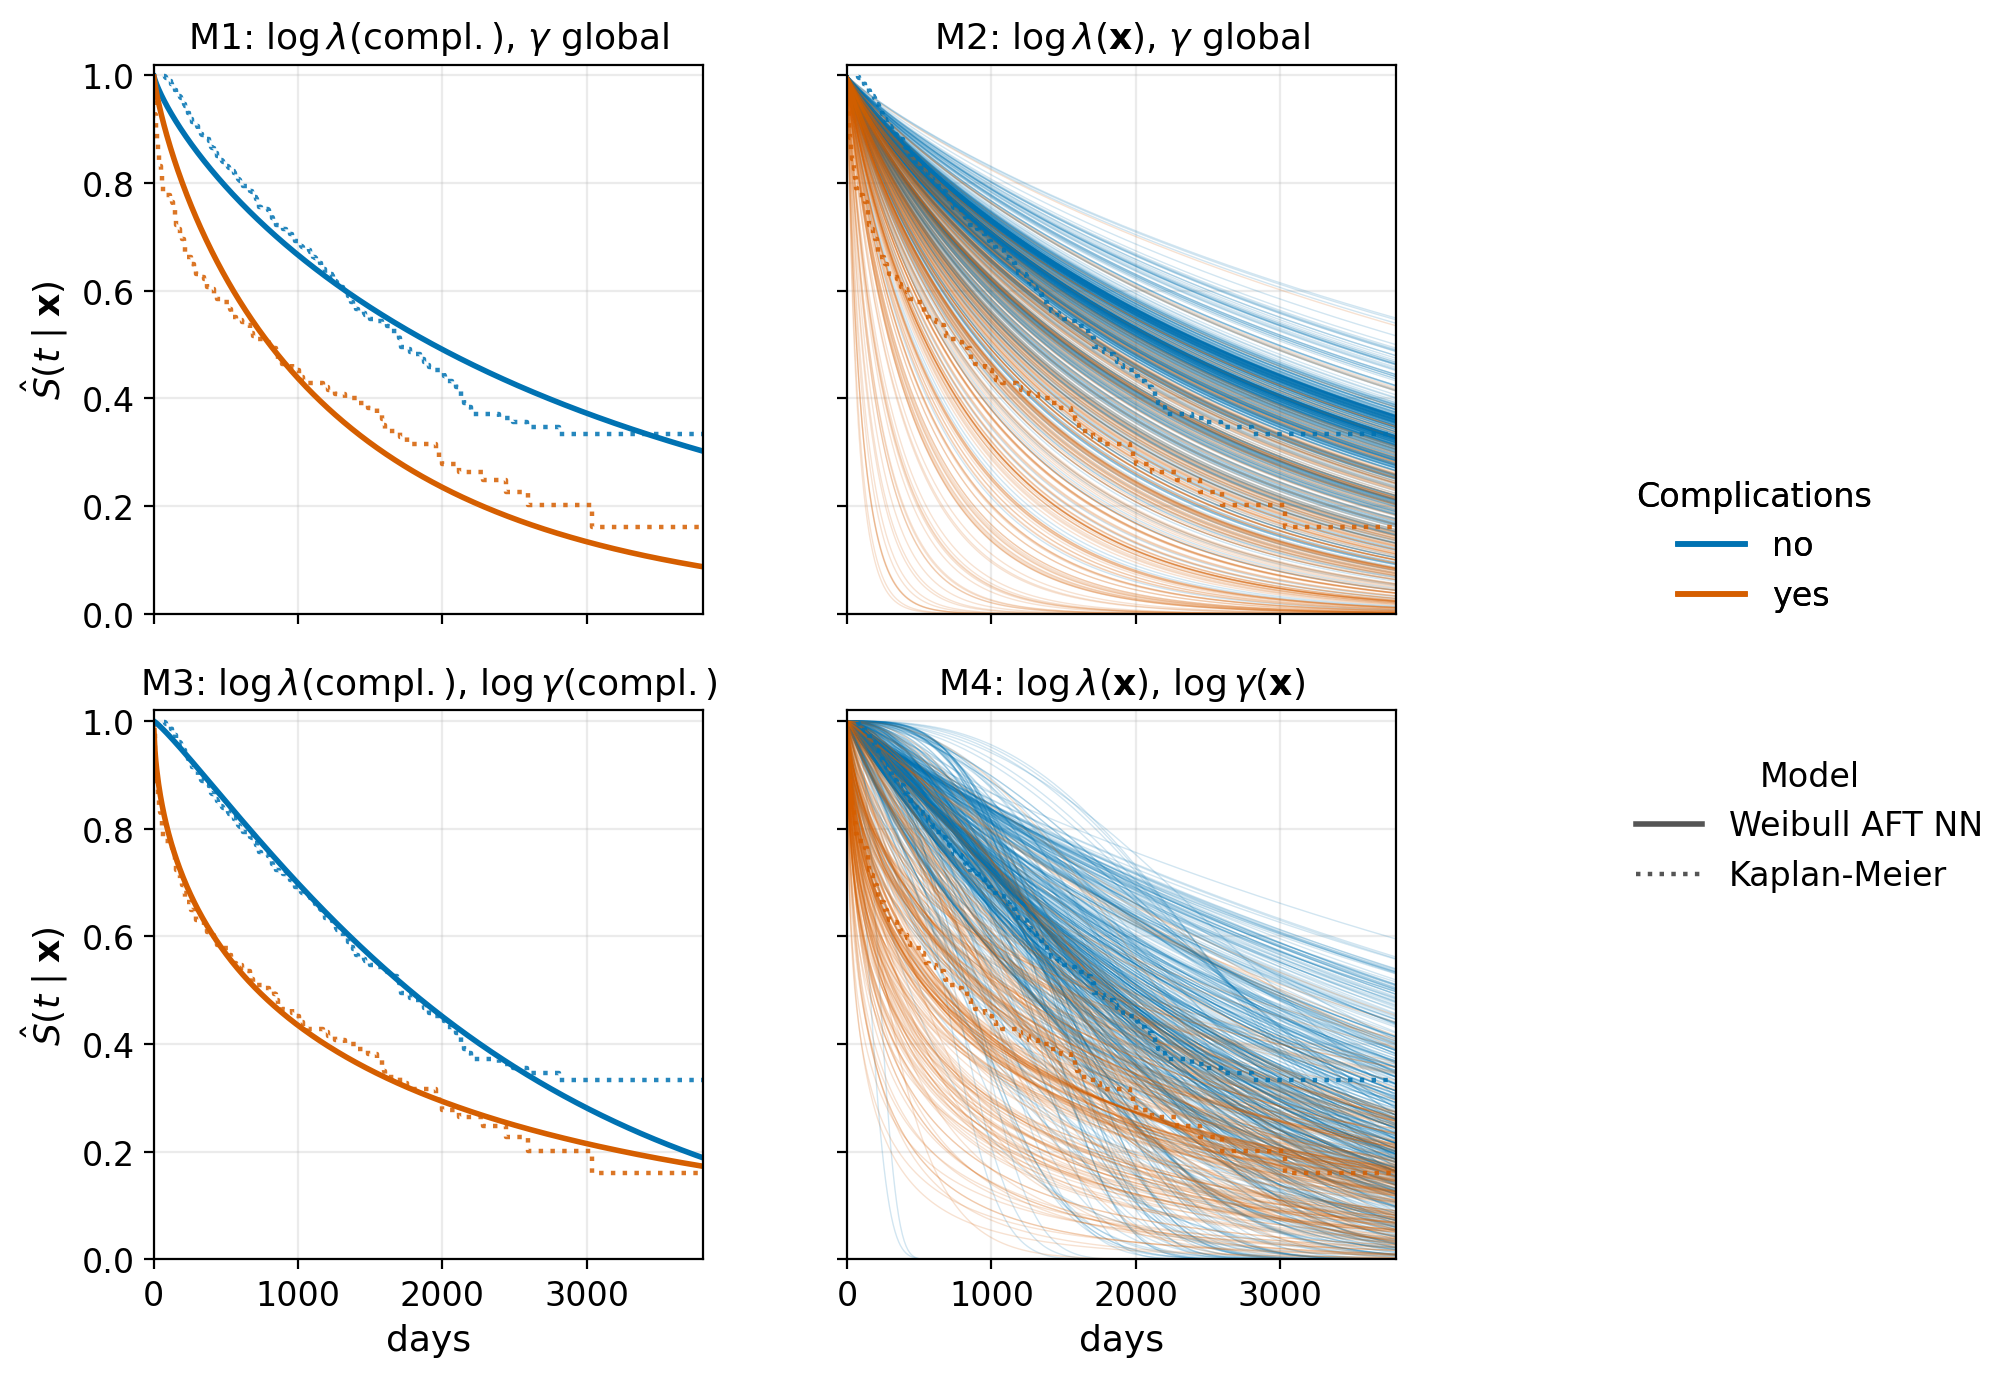
\includegraphics[width=1\linewidth,height=\textheight,keepaspectratio]{Figures/neuralnetworks/fig-p3c17-weibull-aft-nn.png}

}

\caption{\label{fig-p3c17-weibull-aft-nn}Weibull AFT fit to the
\texttt{tumor} data via a neural network, in four increasingly flexible
parameterizations. \emph{Top-left (M1)}: the scale, \(\lambda\), depends
on \texttt{complications}; the shape \(\gamma\) is global.
\emph{Top-right (M2)}: \(\lambda\) depends on all features, \(\gamma\)
is still global; the resulting curves are individualized in scale but
share a common shape. \emph{Bottom-left (M3)}: both \(\lambda\) and
\(\gamma\) depend on \texttt{complications}; the two curves exhibit
different shapes. \emph{Bottom-right (M4)}: both heads are FFNNs over
all seven covariates and produce one Weibull distribution \emph{per
unique feature set}. Each curve is colored by complications status.
Kaplan-Meier estimates are overlaid in each panel for reference.}

\end{figure}%

Figure~\ref{fig-p3c17-weibull-aft-nn} illustrates the general
applicability and flexibility of this method. However, even when an
appropriate survival distribution is selected, predictions remain
constrained by the shape of that distribution's hazard or survival
function. As a result, relatively few neural-network survival models are
fully parametric (Wiegrebe et al. 2024), and even those often attempt to
relax the parametric assumption. One common strategy is to use a
\emph{mixture distribution}. For a sufficiently large number of mixture
components, \(K\), mixtures of Weibull or log-normal distributions can
approximate a wide range of smooth survival distributions while
retaining the practical advantages of a parametric model, including
closed-form survival and hazard functions.

\begin{itemize}
\tightlist
\item
  \emph{DeepWeiSurv} (Bennis, Mouysset, and Serrurier 2020) uses a
  feed-forward encoder to predict the weights
  \(\alpha_k(\mathbf{x}\mid \boldsymbol{\theta})\) and the scale and
  shape parameters of a \(K\)-component Weibull mixture, trained using
  the censored mixture negative
  log-likelihood.\index{neural networks!survival analysis!DeepWeiSurv}
\item
  \emph{DPWTE} (Bennis, Mouysset, and Serrurier 2021) extends this
  construction by adding a sparse Weibull mixture layer whose weights
  are penalized to softly prune unused components during training,
  allowing the effective mixture size to adapt to the
  data.\index{neural networks!survival analysis!DPWTE}
\item
  \emph{Deep Survival Machines} (DSM) (Nagpal, Li, and Dubrawski 2021)
  is the most widely used parametric variant. It generalizes the
  construction to Weibull or log-normal components, adds regularization
  on the mixture weights to prevent component collapse, and extends
  naturally to competing risks through cause-specific heads sharing a
  common
  encoder.\index{neural networks!survival analysis!deep survival machines}
\item
  \emph{Countdown Regression} (Avati et al. 2020) is also parametric but
  evaluates and trains the predicted distribution via a
  \emph{survival-adapted continuous ranked probability score}
  (Chapter~\ref{sec-rules}) rather than the negative
  log-likelihood.\index{neural networks!survival analysis!countdown regression}
\end{itemize}

\subsection{Semi-parametric Cox-based neural
networks}\label{sec-nnet-cox}

The Cox proportional hazards (PH) model
(Section~\ref{sec-classical-cox}) avoids the distributional assumption
by specifying only the relative hazard through a linear predictor
\(\eta_i = \mathbf{x}_i^\top\boldsymbol{\beta}\).\index{neural networks!survival analysis!semi-parametric}
This semi-parametric structure carries over naturally to Cox neural
networks (Cox-NNs) by predicting a scalar risk score
\(g(\mathbf{x}_i \mid \boldsymbol{\theta}) = \eta_i\) and using the
negative Cox partial likelihood (\ref{eq-lpartial}) as the training
objective:\index{neural networks!survival analysis!Cox neural networks}

\begin{equation}\phantomsection\label{eq-nnet-cox-loss}{
-\ell_{PL}(\boldsymbol{\theta}) = -\sum_{k=1}^m \left(g(\mathbf{x}_{i_{(k)}} \mid \boldsymbol{\theta}) - \log \left(\sum_{j \in \mathcal{R}_{t_{(k)}}} \exp(g(\mathbf{x}_j \mid \boldsymbol{\theta}))\right)\right),
}\end{equation}

where \(\mathcal{R}_{t_{(k)}}\) is the risk set at the \(k\)th ordered
event time, \(t_{(k)}\), for \(m \leq n\) unique event times (assuming
no ties).

This loss is differentiable in \(\boldsymbol{\theta}\) and can be
minimized by backpropagation. To obtain a full predicted survival
distribution from the risk score
\(\hat{\eta}_i = g(\mathbf{x}_i \mid \hat{\boldsymbol{\theta}})\), the
Breslow estimator of the baseline cumulative hazard \(\hat{H}_0\)
(\ref{eq-breslow}) is combined with \(\hat{\eta}_i\), exactly as in the
standard Cox model (Section~\ref{sec-classical-cox}).
\index{Cox proportional hazards}\index{Cox proportional hazards!Breslow estimator}

One practical complication is that the inner sum in
(\ref{eq-nnet-cox-loss}) ranges over the \emph{entire} risk set
\(\mathcal{R}_{t_{(k)}}\), which is not compatible with mini-batch
gradient descent of Algorithm 3 and can become prohibitively expensive
on large or multimodal datasets. A common fix is \emph{risk-set
sub-sampling}: instead of taking the full risk set
\(\mathcal{R}_{t_{(k)}}\) at each event, the risk set is restricted to
the subjects in the current mini-batch, which yields a stochastic
estimate of the partial-likelihood gradient (Kvamme, Borgan, and Scheel
2019). \index{risk-set sub-sampling}

Figure~\ref{fig-p3c17-cox-nn-tumor} illustrates this method using two
Cox-NN variants on the \texttt{tumor} dataset with the reference FFNN
architecture of Figure~\ref{fig-p3c17-ffnn-arch}, and again with the
Kaplan-Meier estimate (dotted lines) stratified by
\texttt{complications}. Both models are trained by minimizing
(\ref{eq-nnet-cox-loss}), and the predicted survival curves are obtained
by combining the Breslow estimator (\ref{eq-breslow}) with the fitted
risk scores.

\begin{itemize}
\tightlist
\item
  \textbf{C1}: The risk score depends only on the single covariate
  \texttt{complications}; yielding two predicted survival curves that
  broadly follow the Kaplan-Meier estimates.
\item
  \textbf{C2}: The risk score depends on all seven covariates. The
  proportional hazards assumption is visible: despite the individualized
  predictions, all curves share the same baseline shape and do not
  cross.
\end{itemize}

To relax the proportional-hazards assumption, one can either introduce
stratification (estimating separate baseline hazards for predefined
groups) or allow covariate effects to vary over time.
\index{time-varying covariates} A neural-network implementation of the
latter is discussed below.

\begin{figure}

\centering{

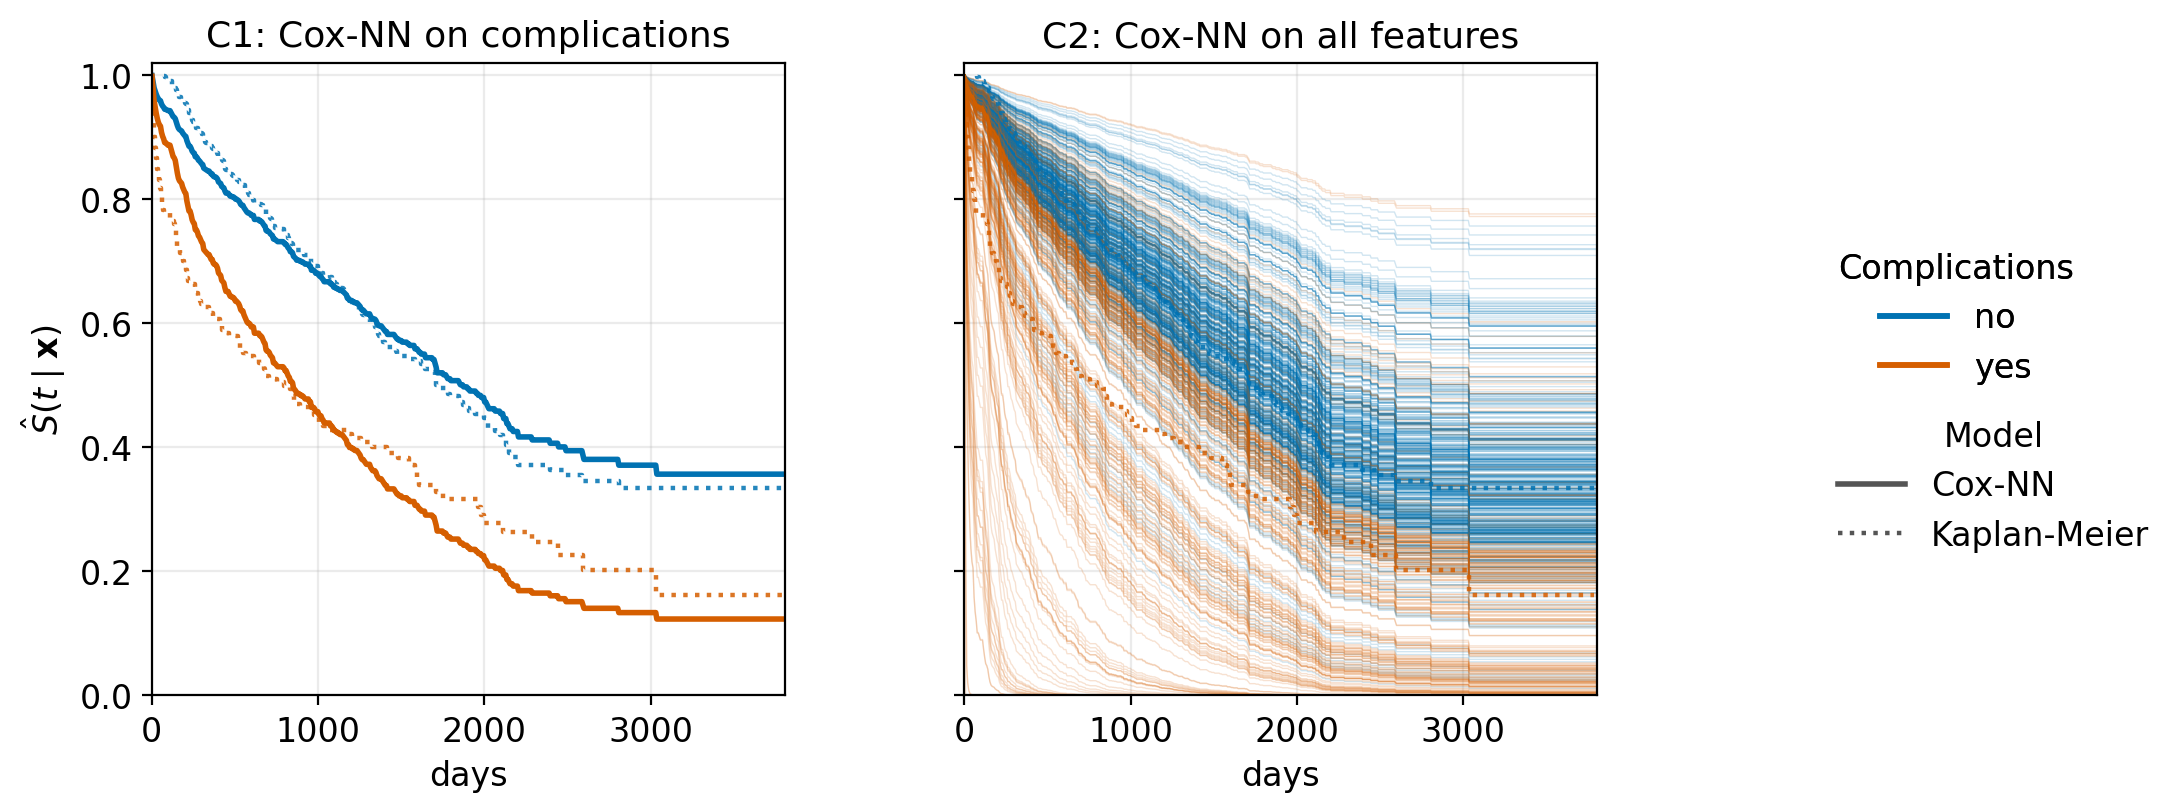
\includegraphics[width=1\linewidth,height=\textheight,keepaspectratio]{Figures/neuralnetworks/fig-p3c17-cox-nn-tumor.png}

}

\caption{\label{fig-p3c17-cox-nn-tumor}Cox-NN fits to the \texttt{tumor}
data with survival curves recovered via the Breslow baseline cumulative
hazard (\ref{eq-breslow}). \textbf{C1}: risk score on the single
covariate \texttt{complications} --- two predicted survival curves, one
per complications group. \textbf{C2}: risk score on all seven covariates
--- one predicted survival curve per patient, colored by complications
status. Dotted curves in both panels show the Kaplan-Meier estimate
stratified by \texttt{complications} for reference. Both models assume
proportional hazards: by construction the per-patient curves in
\textbf{C2} are scaled versions of a single baseline shape.}

\end{figure}%

Several concrete implementations have been suggested using a Cox-based
approach.

\begin{itemize}
\tightlist
\item
  \textbf{DeepSurv} (Katzman et al. 2018) uses a feed-forward risk score
  trained on (\ref{eq-nnet-cox-loss}) with mini-batch risk-set
  sub-sampling. It is essentially the C2 model
  (Figure~\ref{fig-p3c17-cox-nn-tumor}, right) with more freedom on
  depth and weight-decay regularization, and serves as the standard
  baseline in modern Cox-NN
  comparisons.\index{neural networks!survival analysis!DeepSurv}
\item
  \textbf{Cox-nnet} (Ching, Zhu, and Garmire 2018) is a contemporary
  alternative to DeepSurv, using the same underlying model, but tuned
  for high-dimensional omics inputs (regularized training, dropout,
  gene-level interpretability
  heuristics).\index{neural networks!survival analysis!Cox-nnet}
\item
  \textbf{Cox-Time} (Kvamme, Borgan, and Scheel 2019) lets the effect of
  \(\mathbf{x}\) depend on time,
  \(\eta(\mathbf{x}_i, t) = g(\mathbf{x}_i, t \mid \boldsymbol{\theta})\),
  so that the predictor produces \emph{time-varying covariate effects}
  rather than a single constant log hazard ratio. The
  proportional-hazards constraint of (\ref{eq-nnet-cox-loss}) is relaxed
  whenever the network exploits this time-dependence; within a
  non-linear architecture, this lets the implied log hazard ratio
  between two feature sets change with \(t\) rather than being a
  constant. This model is illustrated in
  Figure~\ref{fig-p3c17-coxtime-tumor} with the risk score dependent on
  \texttt{complications} only (left) and all features (right). Unlike
  the Cox-NN curves in Figure~\ref{fig-p3c17-cox-nn-tumor}, the
  predicted survival curves are no longer constrained to be scaled
  versions of a common baseline
  shape.\index{neural networks!survival analysis!Cox-Time}
\item
  \textbf{Deep Cox Mixtures} (Nagpal et al. 2021) relaxes proportional
  hazards by combining \(K\) Cox PH sub-models in a per-subject
  \emph{mixture}. For each subject, a shared FFNN predicts the mixture
  weights \(\alpha_k(\mathbf{x}\mid \boldsymbol{\theta})\) and \(K\)
  component-specific risk scores
  \(\eta_k(\mathbf{x}\mid \boldsymbol{\theta})\); each component has its
  own baseline hazard estimated non-parametrically. Because the \(K\)
  baseline hazards can differ, the resulting model is not restricted to
  proportional
  hazards.\index{neural networks!survival analysis!Deep Cox Mixtures}
\item
  \textbf{Imaging-, omics- and graph-based Cox variants}
  (DeepConvSurv\index{neural networks!survival analysis!DeepConvSurv}
  (Zhu, Yao, and Huang 2016),
  Cox-PASNet\index{neural networks!survival analysis!Cox-PASNet} (Hao et
  al. 2018), VAECox\index{neural networks!survival analysis!VAECox} (Kim
  et al. 2020),
  DeepOmix\index{neural networks!survival analysis!DeepOmix} (Lianhe
  Zhao et al. 2021),
  BioFusionNet\index{neural networks!survival analysis!BioFusionNet}
  (Mondol et al. 2024), and others) replace the FFNN risk score with a
  domain-appropriate encoder (CNN on whole-slide pathology, VAE on RNA
  sequence data, graph attention on gene networks, transformer on
  multimodal inputs) while keeping (\ref{eq-nnet-cox-loss}) as the
  training objective.
\end{itemize}

\begin{figure}

\centering{

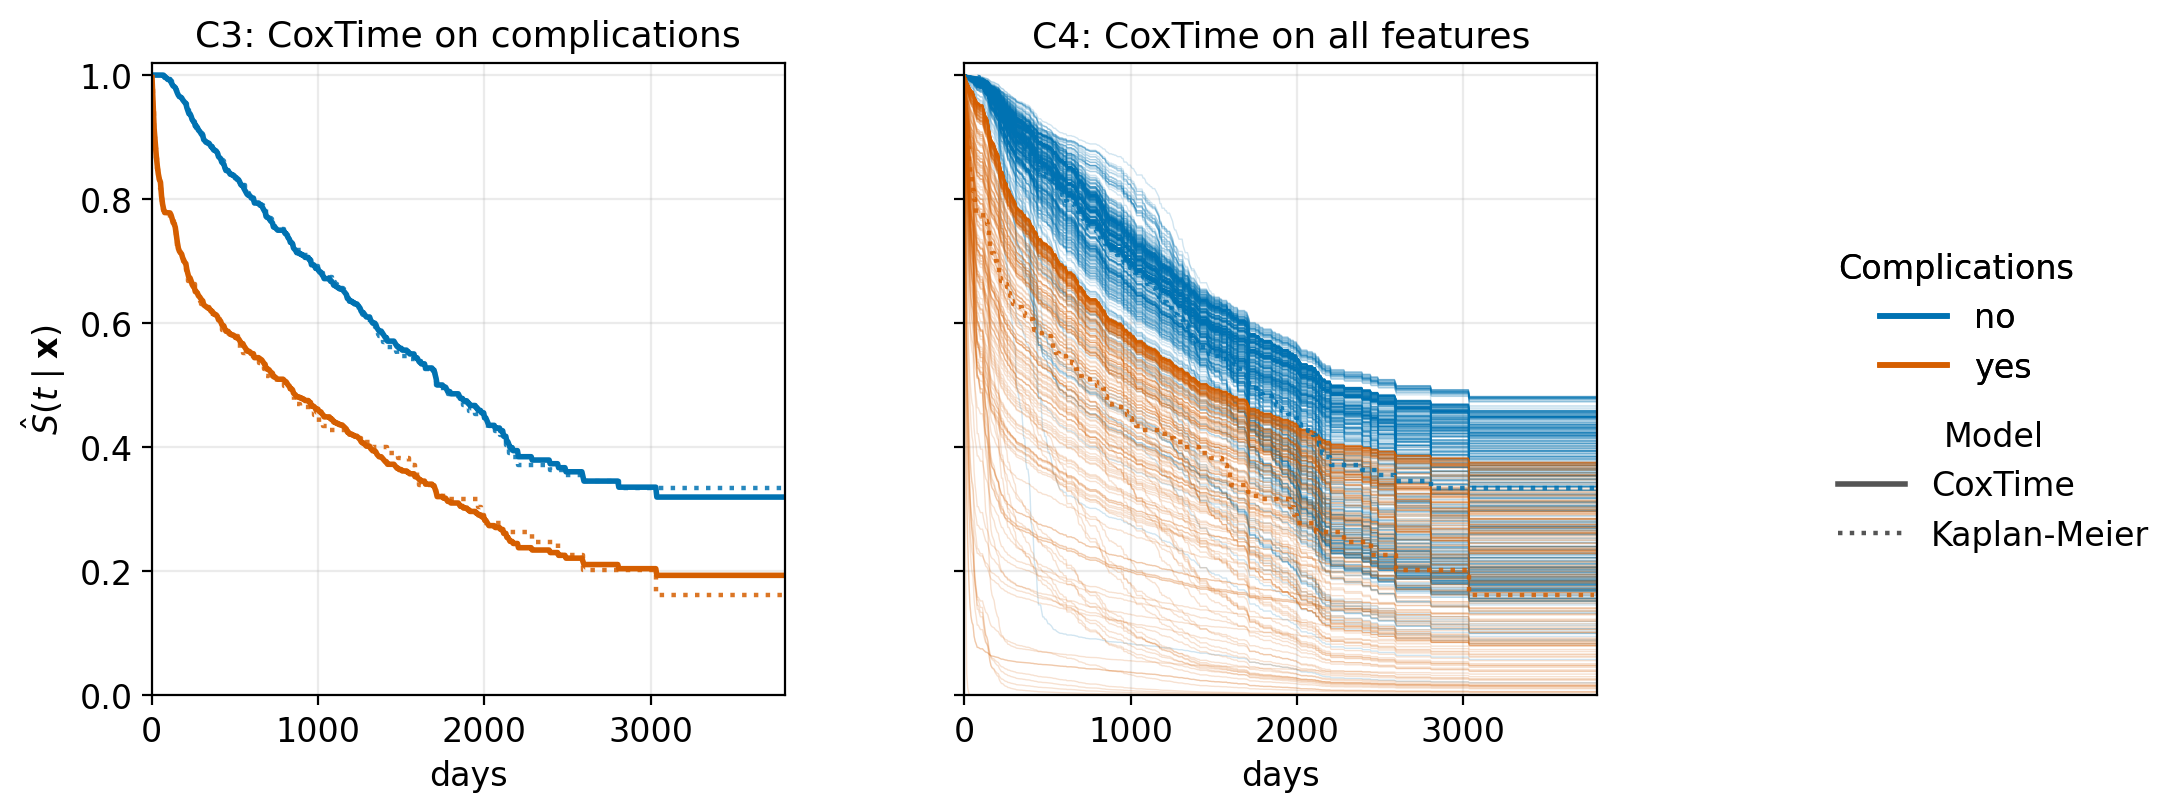
\includegraphics[width=1\linewidth,height=\textheight,keepaspectratio]{Figures/neuralnetworks/fig-p3c17-cox-time-tumor.png}

}

\caption{\label{fig-p3c17-coxtime-tumor}CoxTime fits to the
\texttt{tumor} data using the same FFNN architecture as
Figure~\ref{fig-p3c17-ffnn-arch}, but trained with the time-varying
partial likelihood of Cox-Time so the predictor allows the effect of
\(\mathbf{x}\) to drift with \(t\). \textbf{C3}: CoxTime with
\texttt{complications} only (analogous to the Weibull M3); the two
predicted curves no longer share a common baseline shape and the gap
between them changes with \(t\). \textbf{C4}: CoxTime with all seven
features (analogous to the Weibull M4); per-patient curves are no longer
constrained to share a common baseline shape. Dotted curves:
Kaplan-Meier estimate stratified by \texttt{complications}.}

\end{figure}%

\section{Reduction-based neural networks}\label{sec-nnet-reduction}

The final category of survival neural networks discussed here
\emph{reduces} the survival task to a classification or regression
problem through data transformation, after which a standard neural
network is trained on the transformed task (Wiegrebe et al.
2024).\index{neural networks!survival analysis!reductions}
Survival-specific challenges, such as censoring, are all handled
entirely by the reduction step. The neural network itself is an ordinary
regressor or classifier, meaning any of the architectures from
Section~\ref{sec-nnet-beyond-ffnn} can be used without further
modification.

As reduction is introduced in detail in Part IV, common models using
this method are only briefly mentioned here.

\begin{itemize}
\tightlist
\item
  \textbf{Pseudo-value reduction.} Pseudo-values\index{pseudo-values}
  (Chapter~\ref{sec-pseudo-value-reduction}) replace censored event
  times with jackknife-style `pseudo-observations' of a target
  functional (for example, the survival probability or restricted mean
  survival time), converting the survival task into regression. Examples
  include:

  \begin{itemize}
  \tightlist
  \item
    \emph{DNNSurv} (Lili Zhao and Feng 2020a), which regresses
    pseudo-values of \(S(\tau)\) on covariates using an
    FFNN;\index{neural networks!survival analysis!DNNSurv}
  \item
    \emph{DeepPseudo} (M. M. Rahman et al. 2021), which extends the
    approach to competing risks through pseudo-values of the
    cause-specific cumulative incidence functions;
    and\index{neural networks!survival analysis!DeepPseudo}
  \item
    \emph{msPseudo} (M. M. Rahman and Purushotham 2022), which further
    generalizes the framework to multi-state outcomes through
    pseudo-values of state-occupation
    probabilities.\index{neural networks!survival analysis!msPseudo}
  \end{itemize}
\item
  \textbf{Discrete-time reduction.} Time is divided into \(J\)
  intervals, with each interval corresponding to the binary
  classification task ``does the event occur in this
  interval?''\index{discrete-time survival analysis}
  (Chapter~\ref{sec-partition-based-reductions}). A neural network
  predicts a length-\(J\) vector of conditional discrete hazards
  (\ref{eq-discrete-hazard}), from which the survival function is
  recovered as a running product (\ref{eq-discrete-surv-prob}). Some
  methods include:

  \begin{itemize}
  \tightlist
  \item
    \emph{PLANN} (Biganzoli et al. 1998), which uses a
    single-hidden-layer FFNN on the long-format
    dataset;\index{neural networks!survival analysis!PLANN}
  \item
    \emph{Nnet-survival} (Michael F. Gensheimer and Narasimhan 2019b),
    which predicts discrete hazards using a deep
    network;\index{neural networks!survival analysis!Nnet-survival}
  \item
    \emph{N-MTLR} (Fotso 2018), which adapts multi-task logistic
    regression to
    survival;\index{neural networks!survival analysis!N-MTLR} and
  \item
    \emph{DeepHit} (C. Lee et al. 2018), which jointly models \(Q\)
    competing risks through a softmax over \((J \times (Q{+}1))\)
    cells.\index{neural networks!survival analysis!DeepHit}
  \end{itemize}
\item
  \textbf{Piecewise-exponential reduction.} Time is again partitioned
  into intervals, but the hazard is assumed constant in each
  interval\index{reduction!partition reduction!piecewise exponential model}
  (Section~\ref{sec-piecewise-constant-hazards}). The resulting
  likelihood is equivalent to a Poisson
  regression\index{Poisson regression} on a long-format dataset with
  offsets equal to the exposure time in each interval. Examples include:

  \begin{itemize}
  \tightlist
  \item
    \emph{PC-Hazard} (Kvamme and Borgan 2021), which predicts
    piecewise-constant hazards on a fine event-time grid using an FFNN
    trained against the Poisson-equivalent loss;
    and\index{neural networks!survival analysis!PC-Hazard}
  \item
    \emph{DeepPAMM} (Kopper et al. 2021, 2022), which combines
    interpretable structured effects with deep learning components for
    high-dimensional or unstructured inputs through
    \emph{semi-structured distributional regression} (Rügamer, Kolb, and
    Klein 2024).\index{neural networks!survival analysis!DeepPAMM}
  \end{itemize}
\end{itemize}

\section{Conclusion}\label{conclusion-12}

\begin{tcolorbox}[enhanced jigsaw, toprule=.15mm, bottomtitle=1mm, opacityback=0, breakable, leftrule=.75mm, title={Key takeaways}, toptitle=1mm, bottomrule=.15mm, colback=white, colframe=quarto-callout-warning-color-frame, titlerule=0mm, opacitybacktitle=0.6, coltitle=black, rightrule=.15mm, left=2mm, colbacktitle=quarto-callout-warning-color!10!white, arc=.35mm]

\begin{itemize}
\tightlist
\item
  Neural networks are flexible machine-learning models that learn
  complex relationships directly from the data through gradient-based
  optimization, making them particularly useful when relationships are
  highly non-linear or the input data are high-dimensional.
\item
  Survival neural networks are obtained by combining a neural-network
  architecture with a survival-aware loss function or data
  transformation. Three broad frameworks dominate the literature:
  parametric neural networks, semi-parametric Cox-based neural networks,
  and reduction-based neural networks.
\item
  Modern neural-network architectures (FFNNs, CNNs, RNNs, transformers,
  and others) differ primarily in the types of data and patterns they
  are designed to model, but can usually be incorporated into any of the
  three survival frameworks.
\item
  Neural networks typically require substantially more data,
  computation, and hyperparameter tuning than classical survival models,
  and their predictions are often more difficult to interpret.
\item
  Despite rapid methodological development, many deep learning survival
  methods remain focused on single-event right-censored data; extensions
  to more complex settings such as left-truncation, interval-censoring,
  and event history analysis remain comparatively underdeveloped
  (Wiegrebe et al. 2024).
\end{itemize}

\end{tcolorbox}

\begin{tcolorbox}[enhanced jigsaw, toprule=.15mm, bottomtitle=1mm, opacityback=0, breakable, leftrule=.75mm, title={Further reading}, toptitle=1mm, bottomrule=.15mm, colback=white, colframe=quarto-callout-tip-color-frame, titlerule=0mm, opacitybacktitle=0.6, coltitle=black, rightrule=.15mm, left=2mm, colbacktitle=quarto-callout-tip-color!10!white, arc=.35mm]

\begin{itemize}
\tightlist
\item
  Goodfellow, Bengio, and Courville (2016) and Bishop (2006) for
  general-purpose treatments of neural networks and deep learning,
  complemented by Prince (2023) as a modern reference.
\item
  G. H. Chen (2024) for a self-contained introduction to deep survival
  analysis, covering classical and modern approaches including competing
  risks and dynamic settings.
\item
  Wiegrebe et al. (2024) for a comprehensive review of deep learning for
  survival analysis covering architectures, loss functions and benchmark
  comparisons; the companion table at
  \url{https://survival-org.github.io/DL4Survival} indexes over 60
  methods along the taxonomy used in this chapter.
\end{itemize}

\end{tcolorbox}

\chapter{Choosing Models}\label{sec-choosing-models}

In contrast to measure selection, selecting models is more
straightforward and the same heuristics from regression and
classification largely apply to survival analysis. First, for
low-dimensional data\index{low-dimensional data}, many experiments have
demonstrated that machine learning may not improve upon more standard
statistical methods (Christodoulou et al. 2019) and the same holds for
survival analysis (Burk et al. 2026). Therefore, the cost that comes
with using machine learning --- lower interpretability and longer
training times --- is unlikely to provide any performance benefits when
a dataset has relatively few covariates especially when combined with
low sample size. In settings where machine learning is more useful, the
choice largely falls into the four model classes discussed in this book:
random survival forests, survival support vector machines, gradient
boosting machines, and neural networks (deep learning). In benchmark
experiments with sufficient data and computational resources, it is
sensible to include models of varying complexity, from featureless and
linear models to models that capture non-linear effects and
interactions. However, without significant resources, the rules-of-thumb
below can provide a starting point for smaller experiments.

Random survival forests and boosting methods are strong all-purpose
methods that can handle different censoring types and competing risks
settings.\index{random survival forests}\index{gradient boosting machines}
In single-event settings, both have been shown to perform well on
high-dimensional data, outperforming other model classes (Spooner et al.
2020).\index{high-dimensional data} Forests often work well without
hyperparameter tuning and may therefore be a sensible first choice for
high-dimensional data.

Survival support vector machines have generally shown limited empirical
success and appear to have seen little real-world adoption; moreover,
their runtime can be substantial, taking hours to produce models that
may see little (if any) benefit over simpler models (Burk et al. 2026;
Fouodo et al. 2018; Pölsterl, Navab, and Katouzian 2015). Consequently,
they are not generally recommended as a first-choice
method.\index{survival support vector machines}

Among machine learning methods, deep learning has become the dominant
paradigm across many domains, and current research trends point to a
similar trajectory in survival analysis (Wiegrebe et al.
2024).\index{neural networks} Neural network performance remains highly
data-dependent. There are clear situations in which they are preferred
or required, for example when handling image data such as MRI scans, or
when identifying patterns in very large datasets such as omics data, yet
there are no firm heuristics for selecting one architecture over
another.

While deep learning has traditionally required large amounts of data,
this constraint is increasingly relaxed by \emph{transfer learning}, in
which large \emph{pre-trained} models are \emph{fine-tuned} to a
specific context, making powerful architectures usable on smaller
datasets, particularly for feature extraction.\index{transfer learning}
This is especially valuable in multimodal settings, where image or text
inputs are combined with tabular covariates.\index{multimodal data} The
development of \emph{foundation models} opens further avenues,
potentially leveraging general representations to benefit low-resource
time-to-event problems.\index{foundation models} A recent example is
prior-data fitted networks (PFNs), which learn to approximate Bayesian
inference so that predictions can be obtained in a single forward pass.
PFNs have been adapted to right-censored time-to-event data, enabling
individualized survival prediction without dataset-specific training or
tuning (Seletkov et al. 2026; S. Qi et al.
2026).\index{prior-data fitted network}

In practice, many real-world applications go beyond one-off analyses and
require custom architectures developed with frameworks such as PyTorch
(Paszke et al. 2017) or TensorFlow (Abadi et al. 2015) rather than
off-the-shelf implementations.

\subsubsection*{Interpreting survival
models}\label{interpreting-survival-models}

Interpreting models is increasingly important as practitioners rely on
more complex black box models (Molnar 2019). Classic methods for model
comparison, such as the AIC and BIC, have been extended to survival
models, though their application is limited to the core survival models
(Chapter~\ref{sec-classical}) only (Liang and Zou 2008; Volinsky and
Raftery
2000).\index{interpretable machine learning}\index{AIC}\index{BIC} As a
more flexible alternative, any of the calibration measures in
Chapter~\ref{sec-eval-distr-calib} can be used to evaluate a model's fit
to data.\index{calibration} To assess algorithmic fairness, the majority
of measures discussed in Part II can be used to detect bias in a
survival context (Sonabend et al. 2022).\index{fairness} Widely used
interpretability methods such as SHAP and LIME (Molnar 2019) can be
extended to survival analysis off-the-shelf (Langbein et al. 2025), and
time-dependent extensions also exist to interpret the impact of
variables on the survival probability over time (Krzyziński et al. 2023;
Langbein et al. 2025).\index{SHAP}\index{LIME}

\part{Reduction Techniques}

\chapter{Reductions for Survival
Analysis}\label{sec-reduction-techniques}

This part of the book introduces and formalizes the concept of
\emph{reduction} for survival analysis\index{reductions}. A reduction is
defined as ``a complex problem decomposed into simpler subproblems so
that a solution to the subproblems gives a solution to the complex
problem'' (Beygelzimer et al. 2016). Reduction techniques can simplify
the application of machine learning methods to survival analysis in two
ways: by transforming a survival task to a regression or classification
task, allowing use of standard machine learning methods; and by
transforming an event history analysis task into a set of single-event
tasks, allowing the use of single-event machine learning methods. As
will be seen in the upcoming chapters, the two reduction paradigms can
also be combined.

A reduction is only useful if the resulting predictions remain
statistically meaningful for the original survival task. For example,
some approaches treat the event indicator as a target for a
classification task or directly use the observed time as a target for a
regression task while ignoring the censoring status (Schwarzer, Vach,
and Schumacher 2000). The reduction methods presented in this book are
based on clear theoretical foundations and are constructed so that the
resulting predictions can be meaningfully interpreted for the intended
prediction task. Furthermore, the reductions in the following chapters
do not make strong assumptions about the underlying distribution of
event times and thus have similar advantages to non-parametric
(Section~\ref{sec-classical-nonpar}) and semi-parametric methods
(Section~\ref{sec-classical-cox}). The reductions included here can be
applied to many survival tasks, including competing risks and
multi-state settings (Chapter~\ref{sec-eha}), and can predict the most
common survival prediction types (Chapter~\ref{sec-survtsk}).

The general pipeline for survival reduction techniques is depicted in
Figure~\ref{fig-p4c19-reductions-pipeline}. In the training phase
(Figure~\ref{fig-p4c19-reductions-pipeline}, top), the data are
transformed into a different format with the specifics of the
transformation dependent on the reduction technique and survival task at
hand. Once the data are transformed, the target variable becomes a
one-dimensional vector suitable for a regression or classification task
while still encoding censored event-time information. At this stage, a
standard machine learning model for regression or classification can be
applied to the transformed data without any additional changes to the
model or its implementation. In the prediction phase
(Figure~\ref{fig-p4c19-reductions-pipeline}, bottom), if necessary, the
test data are transformed into the same format as the training data
using any transformation parameters obtained during training. This
yields a dataset that can be passed to the previously learned regression
or classification model to generate predictions. Depending on the
reduction technique and the target quantity, the predictions may require
additional post-processing to obtain the quantity of interest.

\begin{figure}

\centering{

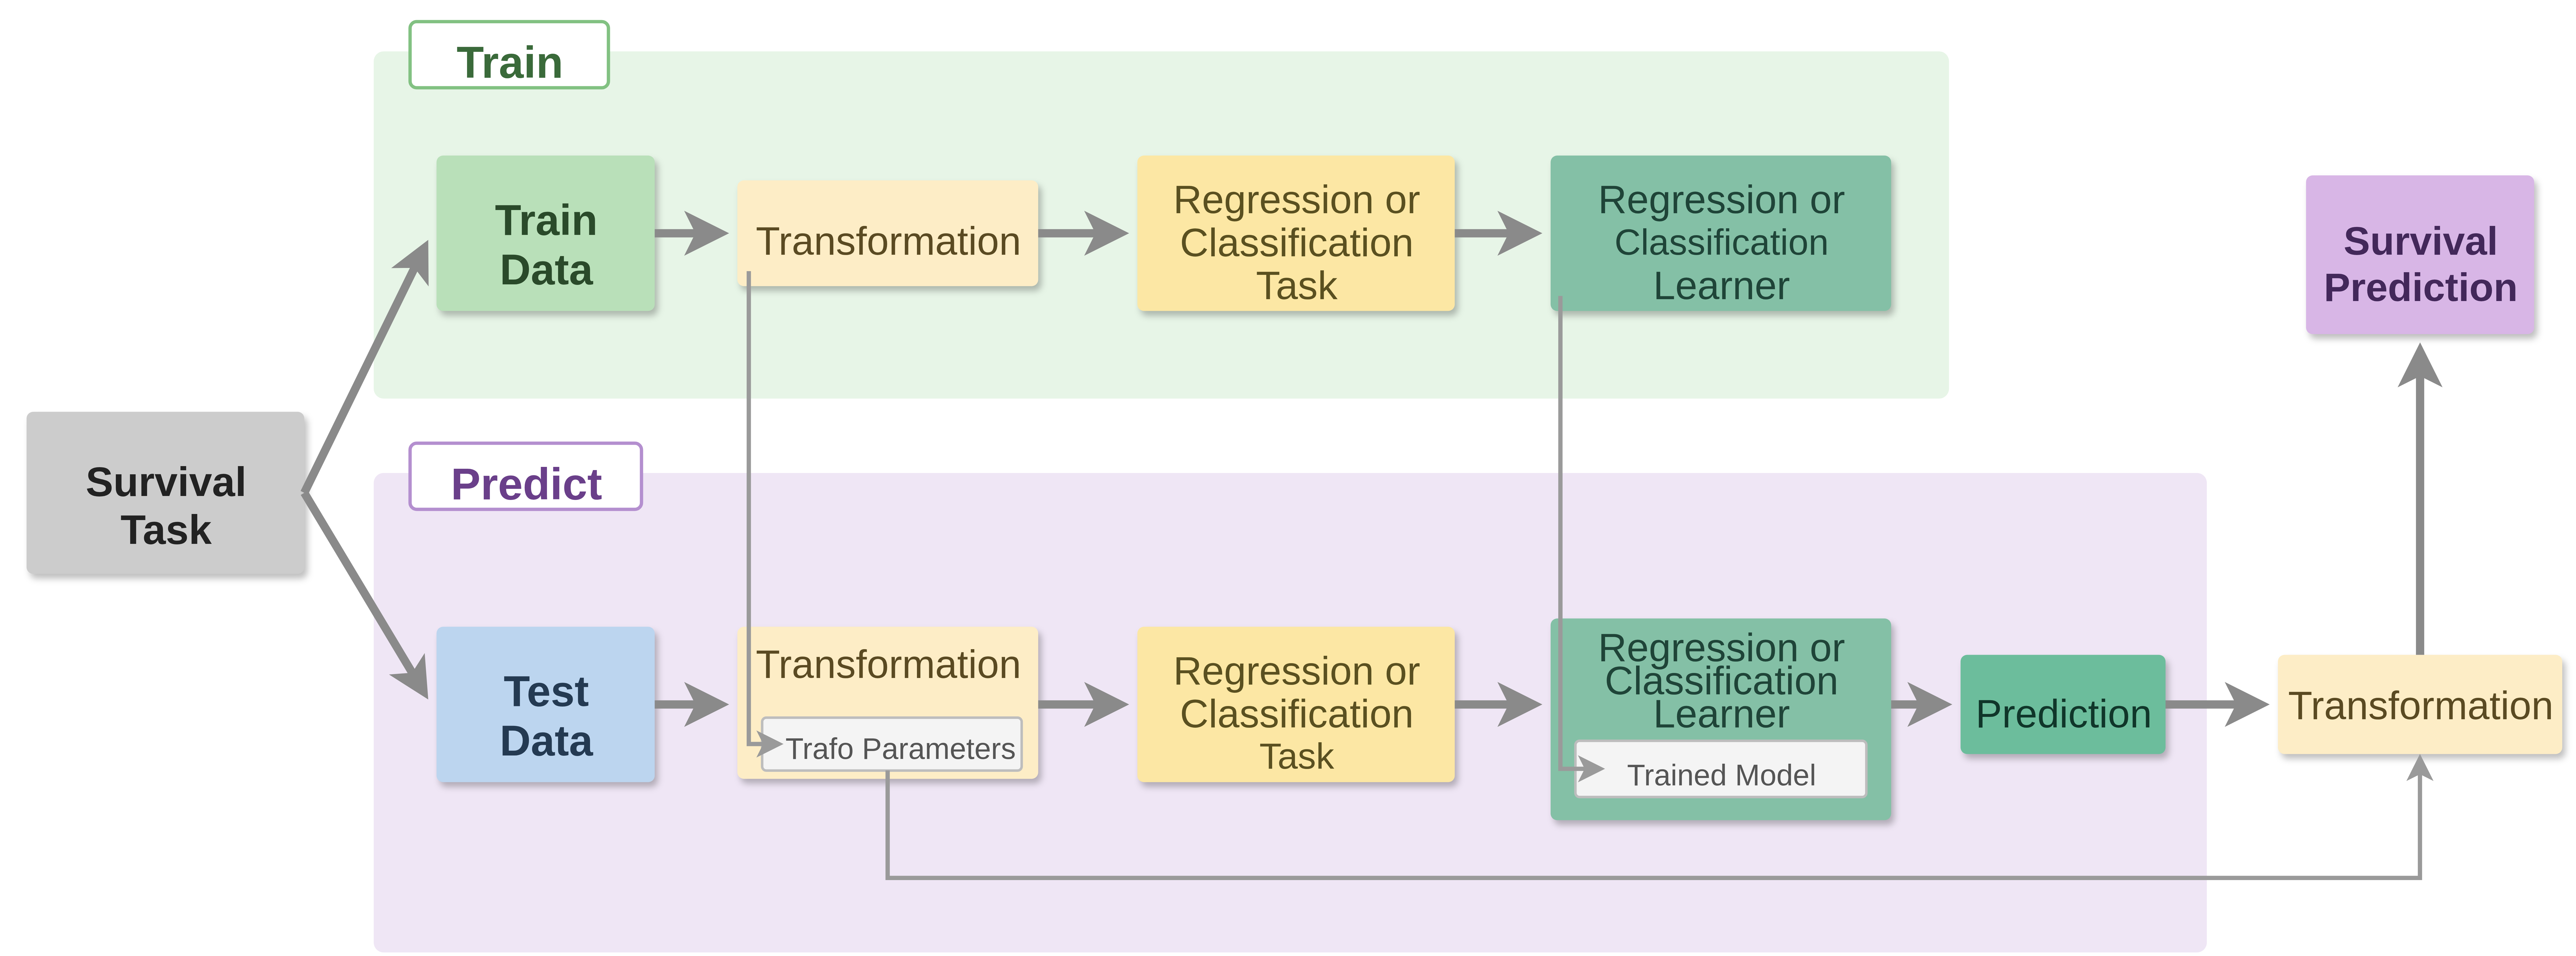
\includegraphics[width=0.9\linewidth,height=\textheight,keepaspectratio]{Figures/reductions/fig-p4c19-reductions-pipeline.png}

}

\caption{\label{fig-p4c19-reductions-pipeline}A general pipeline for
reduction techniques in the context of survival analysis.}

\end{figure}%

The following chapters introduce specific reduction techniques. The
first technique transforms the survival problem to binary classification
to estimate survival probabilities at a set of fixed
times\index{reduction!IPCW classification}
(Chapter~\ref{sec-ipcw-reduction}). This applies to right-censored data
only but is particularly useful when there are only a few time points of
interest, the dataset is very large, or computational resources are
limited. The second reduction transforms the problem into a regression
task\index{reduction!pseudo-value regression}
(Chapter~\ref{sec-pseudo-value-reduction}). Like the classification
approach, this method can estimate survival probabilities at fixed times
but may also be used to estimate many other important quantities,
including the restricted mean survival time, and is also applicable to
event history analysis. However, this flexibility comes at a
computational cost, especially when many time points are considered or
the dataset is large. The partition-based reductions in
Chapter~\ref{sec-partition-based-reductions} aim to estimate the entire
event time distribution rather than a handful of time
points.\index{reduction!partition reductions} They are therefore
particularly useful when complete survival curves or other
distributional summaries are required. Finally,
Chapter~\ref{sec-reductions-eha} introduces reductions that allow event
history analysis to be expressed in terms of single-event tasks, which
allows many of the models in Part III to be applied to competing risks
and multi-state settings.\index{reduction!event history reductions}

An empirical comparison of these reduction techniques, including
benchmark experiments and simulation studies, is provided in Piller et
al. (2026).

\chapter{IPCW Classification}\label{sec-ipcw-reduction}

The inverse probability of censoring weights (IPCW;
Section~\ref{sec-surv-ipcw}) reduction transforms a survival task to a
weighted classification task (Vock et al.
2016).\index{inverse probability of censoring weights} It is applicable
for single-event, right-censored data when the task of interest is to
predict the survival probability at a single time point \(\tau\)
(sometimes referred to as \(\tau\)-year prediction in survival
analysis).\index{reduction!IPCW classification}\index{t-year survival probability@$\tau$-year survival probability}
This method is therefore particularly useful for predicting a single
meaningful time point when the entire survival distribution prediction
is not required. The reduction assumes censoring is marginally
independent of the event time. This reduction is presented in terms of
event probabilities, which are more natural in a classification setting
because the positive class corresponds to the event having occurred.
This is the complement of the usual survival probability, which can be
recovered as \(1\) minus the event probability.

Consider a right-censored dataset
\(\mathcal{D}= \{(\mathbf{x}_i, t_i, \delta_i)\}_{i=1}^n\) with
\(\mathbf{x}_i \in \mathbb{R}^p\) as introduced in
Chapter~\ref{sec-surv}. The probability of an event occurring by time
\(\tau\) is given by the cumulative distribution function,

\[
\Pr(Y \leq \tau \mid \mathbf{x}_i) = F(\tau \mid \mathbf{x}_i) = 1-S(\tau \mid \mathbf{x}_i),
\]

where \(Y\) is the random variable representing the true event time. It
might be tempting to estimate this probability by defining a binary
target variable:

\begin{equation}\phantomsection\label{eq-binary-target}{
e_i(\tau):= \mathbb{I}(t_i \leq \tau \wedge \delta_i = 1),
}\end{equation}

where all observations with event by time \(\tau\) are considered ones
(events) and all other observations zeros (non-events). Using
(\ref{eq-binary-target}), the quantity of interest could naively be
estimated with any binary classification method that outputs
probabilities as \begin{equation}\phantomsection\label{eq-binary-prob}{
\Pr(Y \leq \tau \mid \mathbf{x}_i) = \Pr(e_i(\tau) = 1 \mid \mathbf{x}_i) =: \pi(\mathbf{x}_i;\tau).
}\end{equation}

This approach would only work if there was no censoring before \(\tau\)
in the data. In the presence of censoring, (\ref{eq-binary-target}) does
not define a valid target variable: an observation \(i\) censored before
\(\tau\) is neither an event, nor a confirmed non-event; it is simply
unknown if the event would have occurred had follow-up been allowed to
continue. Removing such observations would introduce a form of selection
bias (Chapter~\ref{sec-intro}), skewing the average survival time to be
longer than in reality, but treating them as events would introduce
another form of bias by artificially increasing the probability of
experiencing the event.

Vock et al. (2016) adapt the estimation procedure to obtain unbiased
estimates of (\ref{eq-binary-prob}) by calculating weights for each
observation,

\begin{equation}\phantomsection\label{eq-adapted-ipc-weights}{
\tilde{w}_i(\tau) = \begin{cases}
0, & \text{if } t_i < \tau \wedge \delta_i = 0,\\
\left[\hat{G}_{KM}(\min(t_i, \tau))\right]^{-1}, & \text{otherwise},
\end{cases}
}\end{equation}

where \(\hat{G}_{KM}\) is the Kaplan-Meier estimate of the censoring
distribution (Section~\ref{sec-surv-ipcw}). Hence, observations censored
before \(\tau\) receive weight zero (thus removed) and the remaining
observations are upweighted to compensate for information loss.

These weights are integrated into the estimation procedure by optimizing
a weighted objective function, allowing the binary target variable in
(\ref{eq-binary-target}) to be used as the target in a weighted
classification problem. Let \(\ell(e_i(\tau), \pi(\mathbf{x}_i;\tau))\)
be some pointwise loss, then any learner that can handle weights (true
for most popular machine learning methods) can be trained to optimize:
\begin{equation}\phantomsection\label{eq-ipcw-loss-weighted}{
L(\pi,\tau) = \sum_{i=1}^n \tilde{w}_i(\tau) \ell(e_i(\tau), \pi(\mathbf{x}_i;\tau)).
}\end{equation}

The exact form of (\ref{eq-ipcw-loss-weighted}) depends on the choice of
learner and objective function. For example, let \(\ell\) be the log
loss,

\[
\ell(e_i(\tau), \pi(\mathbf{x}_i;\tau)) = -\left[e_i(\tau)\log(\pi(\mathbf{x}_i;\tau)) + (1-e_i(\tau))\log(1 - \pi(\mathbf{x}_i;\tau))\right],
\]

then (\ref{eq-ipcw-loss-weighted}) becomes:

\[
L(\pi,\tau) = -\sum_{i=1}^n \tilde{w}_i(\tau) \left[e_i(\tau)\log(\pi(\mathbf{x}_i;\tau)) + (1-e_i(\tau))\log(1 - \pi(\mathbf{x}_i;\tau))\right].
\]

This simple reduction lets practitioners estimate \(\tau\)-year survival
probabilities\index{t-year survival probability@$\tau$-year survival probability}
for right-censored data using classification learners, but several
important aspects warrant consideration. First, while the weighting in
(\ref{eq-ipcw-loss-weighted}) takes into account censoring, the success
of the predictions still depends on the choice of model and loss
function. For example, the estimates might not be well-calibrated if the
chosen loss function does not yield well-calibrated probabilities (like
the hinge loss used by support vector machines). Second, predictions
cannot be evaluated using binary classification metrics as the test data
will still include censored observations. Instead, one should use
survival metrics, such as survival scoring rules\index{scoring rules}
(Chapter~\ref{sec-rules}) and concordance
indices\index{concordance index} (Chapter~\ref{sec-eval-crank}).
Finally, (\ref{eq-adapted-ipc-weights}) implies that contributions of
observations censored before time \(\tau\) are multiplied by zero in
(\ref{eq-ipcw-loss-weighted}). Algorithmically, it may be more efficient
to remove censored observations from the training data to avoid
unnecessary computations of the loss. However, this should only be done
with care, especially when using resampling techniques such as
cross-validation, as censored observations are still required for
evaluation.

\section{Conclusion}\label{conclusion-13}

\begin{tcolorbox}[enhanced jigsaw, toprule=.15mm, bottomtitle=1mm, opacityback=0, breakable, leftrule=.75mm, title={Key takeaways}, toptitle=1mm, bottomrule=.15mm, colback=white, colframe=quarto-callout-warning-color-frame, titlerule=0mm, opacitybacktitle=0.6, coltitle=black, rightrule=.15mm, left=2mm, colbacktitle=quarto-callout-warning-color!10!white, arc=.35mm]

\begin{itemize}
\tightlist
\item
  The IPCW reduction transforms a survival task to a weighted
  classification task and can greatly simplify the estimation of
  survival probabilities at a specific time point of interest by
  enabling binary classification learners to be used.
\item
  Learners that support gradient-based optimization such as gradient
  boosting and deep learning are particularly well suited for this task,
  as they support specification of (custom) loss functions and
  integration of weights.
\item
  Currently, the IPCW approach has only been described in detail for
  right-censored data. Extensions to other settings might be possible,
  but have not yet been explored.
\item
  Extensions to event history analysis have also not been well-explored,
  though an extension to competing risks has been recently proposed (see
  further reading).
\end{itemize}

\end{tcolorbox}

\begin{tcolorbox}[enhanced jigsaw, toprule=.15mm, bottomtitle=1mm, opacityback=0, breakable, leftrule=.75mm, title={Further reading}, toptitle=1mm, bottomrule=.15mm, colback=white, colframe=quarto-callout-tip-color-frame, titlerule=0mm, opacitybacktitle=0.6, coltitle=black, rightrule=.15mm, left=2mm, colbacktitle=quarto-callout-tip-color!10!white, arc=.35mm]

\begin{itemize}
\tightlist
\item
  Vock et al. (2016) provide the main reference where they explicitly
  show how different learners (logistic regression, Bayesian networks,
  decision trees and k-nearest neighbors) can be adapted to obtain
  estimates of the event probability.
\item
  Gonzalez Ginestet et al. (2021) introduce extensions to the competing
  risks setting.
\end{itemize}

\end{tcolorbox}

\chapter{Pseudo-Value Regression}\label{sec-pseudo-value-reduction}

Pseudo-value-based approaches were introduced to survival analysis by
Andersen, Klein, and Rosthøj (2003) and have since gained traction due
to their flexibility and ease of application. This approach allows
standard regression learners to be applied to censored survival data by
transforming the original outcomes into
\emph{pseudo-values}.\index{pseudo-values} The term `pseudo-value'
reflects the fact that these quantities are not identical to the outcome
of interest but behave similarly in
expectation.\index{reduction!pseudo-value regression}

Formally, let \(\psi(\tau \mid \mathbf{x})\) denote the (population)
quantity of interest, for example the survival probability,
\(S(\tau \mid \mathbf{x})\), or restricted mean survival time,
\(\operatorname{RMST}(\tau \mid \mathbf{x})\). Let \(\psi(\tau)\) denote
the corresponding marginal quantity and \(\hat\psi(\tau)\) its estimate,
for example the Kaplan-Meier estimate fitted on all \(n\) observations
in the training data. Let \(\hat\psi^{-i}(\tau)\) denote the same
estimator computed after omitting the \(i\)th observation from the
dataset.

The pseudo-value for observation \(i\) is defined using the jackknife
procedure,\index{jackknife}

\begin{equation}\phantomsection\label{eq-pseudo-value}{
\tilde{y}_i(\tau) = n\hat\psi(\tau) - (n-1)\hat\psi^{-i}(\tau).
}\end{equation}

Computing all pseudo-values,
\(\tilde{y}_1(\tau), \ldots, \tilde{y}_n(\tau)\), requires \(n+1\)
evaluations of the univariate estimator (\(n\) evaluations of
\(\hat\psi^{-i}(\tau)\) and one evaluation of \(\hat\psi(\tau)\)) for
each of the \(m\) time points of interest, resulting in \(m(n+1)\)
evaluations in total. Although this may seem computationally demanding,
univariate estimators are typically very fast to compute, and efficient
approximations have been proposed in the literature (Bouaziz 2023;
Parner, Andersen, and Overgaard 2023). Furthermore, pseudo-value methods
are most commonly used when only a small number of time points are of
interest, so \(m\) is usually small.

A key property of pseudo-values is that under mild conditions on
\(\hat\psi\), the conditional population quantity is well approximated
by the conditional expectation of a pseudo-value, treated as a random
variable in the underlying sample (Andersen, Klein, and Rosthøj 2003;
Andersen and Pohar Perme 2010):

\begin{equation}\phantomsection\label{eq-pseudo-value-expectation-1}{
\psi(\tau \mid \mathbf{x}_i) \;\approx\; \mathbb{E}[\tilde{y}_i(\tau) \mid \mathbf{x}_i].
}\end{equation}

This approximate unbiasedness motivates regressing \(\tilde{y}_i\) on
\(\mathbf{x}_i\) in this reduction. The relationship between features
\(\mathbf{x}_i\) and pseudo-values \(\tilde{y}_i(\tau)\) can then be
learned through regression, with a separate model fitted for a given
time point of interest \(\tau\),

\begin{equation}\phantomsection\label{eq-pseudo-value-expectation-2}{
\mathbb{E}[\tilde{y}_i(\tau)\mid\mathbf{x}_i] = g(\mathbf{x}_i\mid\boldsymbol{\theta}_\tau),
}\end{equation}

where \(g(\mathbf{x}_i\mid \boldsymbol{\theta}_\tau)\) is the model's
output for time point \(\tau\), learned by optimizing the parameters
\(\boldsymbol{\theta}_\tau\), for example,
\(g(\mathbf{x}_i\mid \boldsymbol{\theta}_\tau) = \mathbf{x}_i^\top\boldsymbol{\theta}_\tau\)
for linear regression.\index{linear regression} The parameters
\(\boldsymbol{\theta}_\tau\), and hence the function, differ for each
time point \(\tau\).

It follows from (\ref{eq-pseudo-value-expectation-1}) and
(\ref{eq-pseudo-value-expectation-2}) that the fitted regression models
can be used to make predictions of the quantity of interest conditional
on covariates,

\[
\hat{\psi}(\tau\mid\mathbf{x}_i) \approx \hat{\tilde{y}}_i = g(\mathbf{x}_i\mid\hat{\boldsymbol{\theta}}_\tau).
\]

Going forward, when referring to the fitted model, this notation is
simplified to:

\[
\hat{\psi}(\tau \mid \mathbf{x}_i) = g(\mathbf{x}_i\mid\hat{\boldsymbol{\theta}}_\tau).
\]

Rather than learning \(g(\cdot)\) directly, the model often learns a
\emph{predictor function},
\(\eta(\mathbf{x}_i\mid\boldsymbol{\theta}_\tau)\), combined with a
transformation via a known \emph{response function}, \(r(\cdot)\), such
that

\begin{equation}\phantomsection\label{eq-pseudo-value-response-function}{
g(\mathbf{x}_i\mid\boldsymbol{\theta}_\tau) = r(\eta(\mathbf{x}_i\mid\boldsymbol{\theta}_\tau)).
}\end{equation}

The response function maps the predictor \(\eta\) to the target space
(as with neural networks; Section~\ref{sec-nnet-activations}). Its
inverse \(r^{-1}(\cdot)\) is the \emph{link function}, commonly used in
generalized linear models.\index{link function} A response function is
often required as pseudo-values can take any value on \(\mathbb{R}\) but
the target quantity of interest might be constrained to a smaller set,
for example survival probabilities must be within \([0,1]\). The model
may be estimated with the response function embedded in the fitting
process, as in generalized estimating equations (Hardin and Hilbe 2012),
or the response may be applied to the predictions, as in many machine
learning methods. The choice of response function, and consequences for
estimation and interpretation, are discussed in
Section~\ref{sec-pseudo-value-response-function}.

The following sections introduce two common applications of
pseudo-values: survival probability prediction
(Section~\ref{sec-pseudo-value-S}) and restricted mean survival time
prediction (Section~\ref{sec-pseudo-value-rmst}). Finally,
Section~\ref{sec-pseudo-value-eha} extends this reduction to competing
risks and multi-state models.

\section{Pseudo-values for survival
probabilities}\label{sec-pseudo-value-S}

This section details the use of pseudo-values for survival probability
predictions at selected time
points.\index{reduction!pseudo-value regression!survival probabilities}
For illustration, consider the tumor dataset (introduced in
Table~\ref{tbl-surv-data-tumor}), which contains right-censored data for
\(n=776\) observations on time to death after operation (in days) and
features `age' and `complications', which indicates whether
complications occurred during tumor removal. For this example, a simple
linear model is used for (\ref{eq-pseudo-value-expectation-2}) but any
(machine learning) regression model could be used in practice.

Say a clinician is interested in the conditional survival probability of
tumor patients at time points \(\tau \in \{1000, 2000, 3000\}\) days.
The true quantity of interest is
\(\psi(\tau \mid \mathbf{x}_i) = S(\tau \mid \mathbf{x}_i)\), for which
a commonly used univariate estimator is the Kaplan-Meier estimator,
\(\psi(\tau) = S_{KM}(\tau)\). Pseudo-values are then calculated as

\begin{equation}\phantomsection\label{eq-pseudo-value-calculation-S}{
\tilde{y}_i(\tau) = n\hat{S}_{KM}(\tau) - (n-1)\hat{S}_{KM}^{-i}(\tau).
}\end{equation}

The resulting estimates and calculated pseudo-values are shown for the
first 4 subjects of the data in Table~\ref{tbl-pseudo-value-calculation}
for \(\tau = 1000\) days. While the differences in leave-one-out
Kaplan-Meier estimates may appear small (\(<0.01\) difference), these
lead to larger differences in pseudo-values once plugged into
(\ref{eq-pseudo-value-calculation-S}).

\begin{longtable}[]{@{}
  >{\raggedright\arraybackslash}p{(\linewidth - 14\tabcolsep) * \real{0.1250}}
  >{\raggedleft\arraybackslash}p{(\linewidth - 14\tabcolsep) * \real{0.1250}}
  >{\raggedleft\arraybackslash}p{(\linewidth - 14\tabcolsep) * \real{0.1250}}
  >{\raggedleft\arraybackslash}p{(\linewidth - 14\tabcolsep) * \real{0.1250}}
  >{\raggedleft\arraybackslash}p{(\linewidth - 14\tabcolsep) * \real{0.1250}}
  >{\raggedleft\arraybackslash}p{(\linewidth - 14\tabcolsep) * \real{0.1250}}
  >{\raggedleft\arraybackslash}p{(\linewidth - 14\tabcolsep) * \real{0.1250}}
  >{\raggedleft\arraybackslash}p{(\linewidth - 14\tabcolsep) * \real{0.1250}}@{}}
\caption{Illustration of pseudo-value calculation for the first 4
subjects from the tumor dataset at time point \(\tau = 1000\) days. The
table shows the overall Kaplan-Meier estimate \(\hat{S}_{KM}(\tau)\)
calculated for all \(776\) subjects, the leave-one-out Kaplan-Meier
estimate \(\hat{S}_{KM}^{-i}(\tau)\) (obtained by omitting subject
\(i\)), and the calculated pseudo-value \(\tilde{y}_i(\tau)\). The
features age and complications are not used for the calculation of the
pseudo-values but are included in the regression
step.}\label{tbl-pseudo-value-calculation}\tabularnewline
\toprule\noalign{}
\begin{minipage}[b]{\linewidth}\raggedright
complications
\end{minipage} & \begin{minipage}[b]{\linewidth}\raggedleft
age
\end{minipage} & \begin{minipage}[b]{\linewidth}\raggedleft
\(i\)
\end{minipage} & \begin{minipage}[b]{\linewidth}\raggedleft
\(t_i\)
\end{minipage} & \begin{minipage}[b]{\linewidth}\raggedleft
\(\delta_i\)
\end{minipage} & \begin{minipage}[b]{\linewidth}\raggedleft
\(\hat{S}_{KM}(\tau)\)
\end{minipage} & \begin{minipage}[b]{\linewidth}\raggedleft
\(\hat{S}_{KM}^{-i}(\tau)\)
\end{minipage} & \begin{minipage}[b]{\linewidth}\raggedleft
\(\tilde{y}_i(\tau)\)
\end{minipage} \\
\midrule\noalign{}
\endfirsthead
\toprule\noalign{}
\begin{minipage}[b]{\linewidth}\raggedright
complications
\end{minipage} & \begin{minipage}[b]{\linewidth}\raggedleft
age
\end{minipage} & \begin{minipage}[b]{\linewidth}\raggedleft
\(i\)
\end{minipage} & \begin{minipage}[b]{\linewidth}\raggedleft
\(t_i\)
\end{minipage} & \begin{minipage}[b]{\linewidth}\raggedleft
\(\delta_i\)
\end{minipage} & \begin{minipage}[b]{\linewidth}\raggedleft
\(\hat{S}_{KM}(\tau)\)
\end{minipage} & \begin{minipage}[b]{\linewidth}\raggedleft
\(\hat{S}_{KM}^{-i}(\tau)\)
\end{minipage} & \begin{minipage}[b]{\linewidth}\raggedleft
\(\tilde{y}_i(\tau)\)
\end{minipage} \\
\midrule\noalign{}
\endhead
\bottomrule\noalign{}
\endlastfoot
no & 58 & 1 & 579 & 0 & 0.6175 & 0.6172 & 0.8597 \\
yes & 52 & 2 & 1192 & 0 & 0.6175 & 0.6169 & 1.0600 \\
no & 74 & 3 & 308 & 1 & 0.6175 & 0.6184 & -0.0442 \\
yes & 57 & 4 & 33 & 1 & 0.6175 & 0.6183 & -0.0119 \\
\end{longtable}

A linear model is then fit to these pseudo-values
(Table~\ref{tbl-pseudo-value-calculation}), giving

\begin{equation}\phantomsection\label{eq-pseudo-value-S-lm}{
\hat{S}(\tau \mid \mathbf{x}_i) = \hat{\tilde{y}}_i(\tau) = \mathbf{x}_i^\top\hat{\boldsymbol{\beta}}_{\tau}.
}\end{equation}

To illustrate some of the main advantages of this method, consider
fitting the pseudo-values using a linear model of the form:

\begin{equation}\phantomsection\label{eq-pseudo-value-S-lm-complications}{
\hat{S}(\tau \mid \mathbf{x}_i) = \hat{\beta}_{\tau,0} + \hat{\beta}_{\tau,1} x_{i,1},\quad x_{i,1} = \mathbb{I}(\text{complications}_i = \text{`yes'}),
}\end{equation}

for time points \(\tau \in \{1000, 2000, 3000\}\) days.

The results are shown in Figure~\ref{fig-p4c21-pseudo-lm}, where the
black dots indicate the survival probability predictions from
(\ref{eq-pseudo-value-S-lm-complications}) and the solid curves are
Kaplan-Meier estimates of the survival probabilities stratified by the
`complications' variable. Despite the pseudo-values being computed from
a single, \emph{unstratified} Kaplan-Meier estimator, the predictions
still closely match the \emph{stratified} estimates. The reason is that
a separate regression is fitted at each time point \(\tau\), with the
coefficients estimated independently, so the difference between groups
is free to vary over time. The separation between the curves suggests
the proportional hazards assumption may not hold for this data, which
the pseudo-value approach accommodates naturally, since the group effect
\(\hat{\beta}_{\tau,1}\) is not constrained to be constant across
\(\tau\).

In this example the identity response function is used, so the model
places no constraint on the target space,
\(g(\mathbf{x}\mid\boldsymbol{\theta}_\tau) = \eta(\mathbf{x}\mid\boldsymbol{\theta}_\tau) = \mathbf{x}^\top\boldsymbol{\theta}_\tau\),
and the predictions could in principle fall outside \([0,1]\).
Nonetheless, all of the estimated survival probabilities lay within the
valid range. A practical advantage of this parameterization is that the
fitted coefficients are directly interpretable on the
survival-probability scale, unlike a Cox model, whose coefficients are
interpretable only as hazard ratios. For example,
\(\hat{\beta}_{1000,1} \approx -0.23\), so at \(\tau = 1000\) days the
expected survival probability for patients with complications is around
23 percentage points lower than for those without complications. This
interpretability also carries to other time points, for example at
\(\tau = 2000\) days, \(\hat{\beta}_{2000,1} \approx -0.18\), and at
\(\tau = 3000\) days, \(\hat{\beta}_{3000,1} \approx -0.13\); thus, the
average effect of complications depends on \(\tau\) and decreases over
time (complications have a time-varying
effect).\index{time-varying effects}

\begin{figure}

\centering{

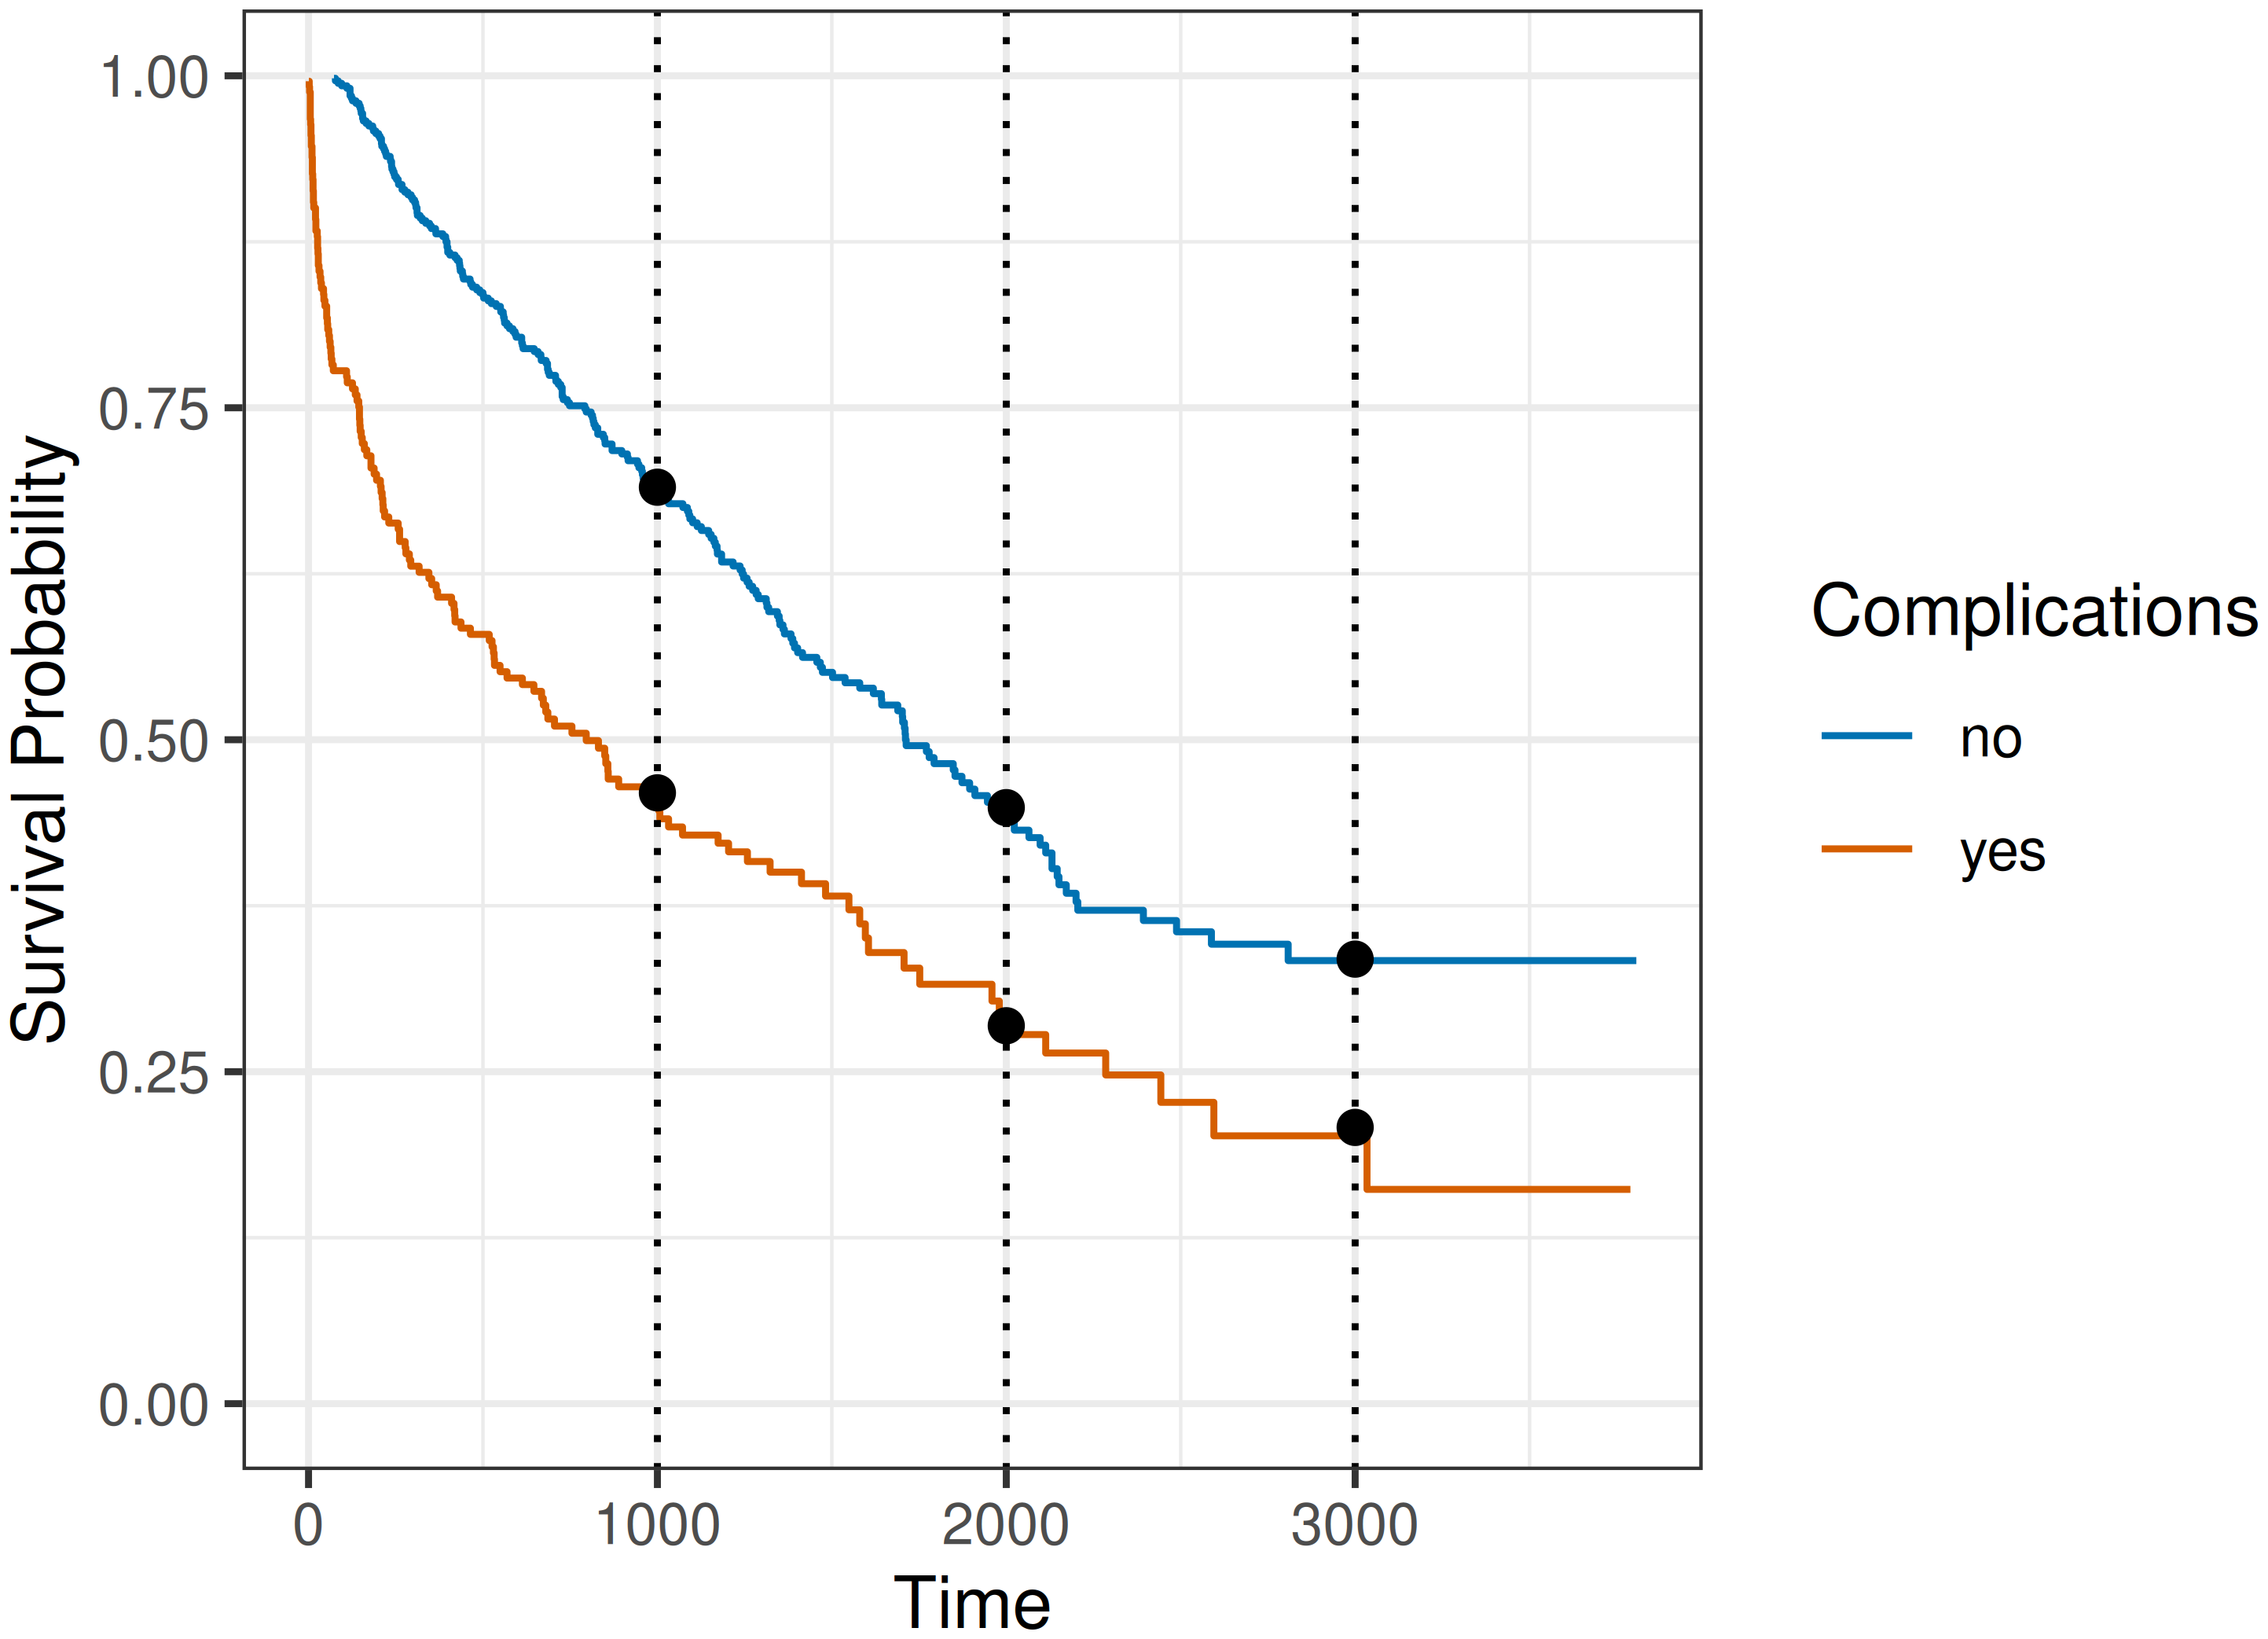
\includegraphics[width=0.6\linewidth,height=\textheight,keepaspectratio]{Figures/survival/fig-p4c21-pseudo-lm.png}

}

\caption{\label{fig-p4c21-pseudo-lm}Comparison of survival probability
estimates from the Kaplan-Meier estimator and a linear model based on
pseudo-values.}

\end{figure}%

In practice, if the data only contained a single, discrete feature, then
a stratified Kaplan-Meier estimator could be used instead of the
pseudo-value approach. Thus, as a final illustration, consider adding
age to the model,

\[
\begin{aligned}
\hat{S}(\tau \mid \mathbf{x}_i) = \hat{\beta}_{\tau,0} + \hat{\beta}_{\tau,1} x_{i,1} + \hat{\beta}_{\tau,2} x_{i,2},\\ \quad x_{i,1} = \mathbb{I}(\text{complications}_i = \text{`yes'}), x_{i,2} = \text{age}_i,
\end{aligned}
\]

and again the response function, \(r(\cdot)\), is the identity function.
The resulting estimates are in Table~\ref{tbl-pseudo-lm-age}, where the
effects of age and complications are calculated for each time point
\(\tau \in \{1000, 2000, 3000\}\) days separately.

\begin{longtable}[]{@{}rrr@{}}
\caption{Estimates of the effects of complications,
\(\hat{\beta}_{\tau,1}\), and age, \(\hat{\beta}_{\tau,2}\), on the
survival probability at different time points
\(\tau \in \{1000, 2000, 3000\}\)
days.}\label{tbl-pseudo-lm-age}\tabularnewline
\toprule\noalign{}
\(\tau\) & \(\hat{\beta}_{\tau,1}\) & \(\hat{\beta}_{\tau,2}\) \\
\midrule\noalign{}
\endfirsthead
\toprule\noalign{}
\(\tau\) & \(\hat{\beta}_{\tau,1}\) & \(\hat{\beta}_{\tau,2}\) \\
\midrule\noalign{}
\endhead
\bottomrule\noalign{}
\endlastfoot
1000 & -0.2205 & -0.0032 \\
2000 & -0.1428 & -0.0070 \\
3000 & -0.1050 & -0.0071 \\
\end{longtable}

Conditional on \(\tau\), the interpretation is equivalent to a standard
multiple linear regression model. For example, at \(\tau = 1000\) days,
the effect of age is \(\hat{\beta}_{1000,2} \approx -0.0032\), which
means that, holding the other covariates fixed, the expected survival
probability is reduced by around 0.32 percentage points per additional
year of age. In contrast, at \(\tau=2000\) days, the survival
probability is reduced by around 0.70 percentage points per additional
year of age (7 percentage points for a 10-year difference), meaning age
has more than double the impact for later time points. Therefore, even
as the number of covariates increases, the pseudo-value approach remains
a highly interpretable reduction.

\section{Pseudo-values for RMST}\label{sec-pseudo-value-rmst}

Another common use for the pseudo-value approach is the restricted mean
survival time (RMST; Chapter~\ref{sec-survtsk}), for which the standard
plug-in estimator is
\index{reduction!pseudo-value regression!restricted mean survival time}\index{restricted mean survival time}

\[
\operatorname{RMST}(\tau) = \int_0^\tau S_{KM}(y) \ \,\mathrm{d}y,
\]

giving the calculated pseudo-values

\[
\tilde{y}_i(\tau) = n \widehat{\operatorname{RMST}}(\tau) - (n-1)\widehat{\operatorname{RMST}}^{-i}(\tau),
\]

where \(\tilde{y}_i(\tau)\) is the pseudo-value of the restricted mean
survival time at time \(\tau\) for observation \(i\).

Continuing the tumor data example from Section~\ref{sec-pseudo-value-S},
consider how the RMST depends on features. The general idea is
illustrated in Figure~\ref{fig-p4c21-pseudo-rmst}, which displays
survival curves for each group (complications vs.~no complications) with
the RMST shown as the area under the curve up to \(\tau = 1000\) days.
Thus, within the first 1000 days after operation, patients with
complications are expected to live 246 days less than patients without
complications (the difference between the areas under the two curves).

\begin{figure}

\centering{

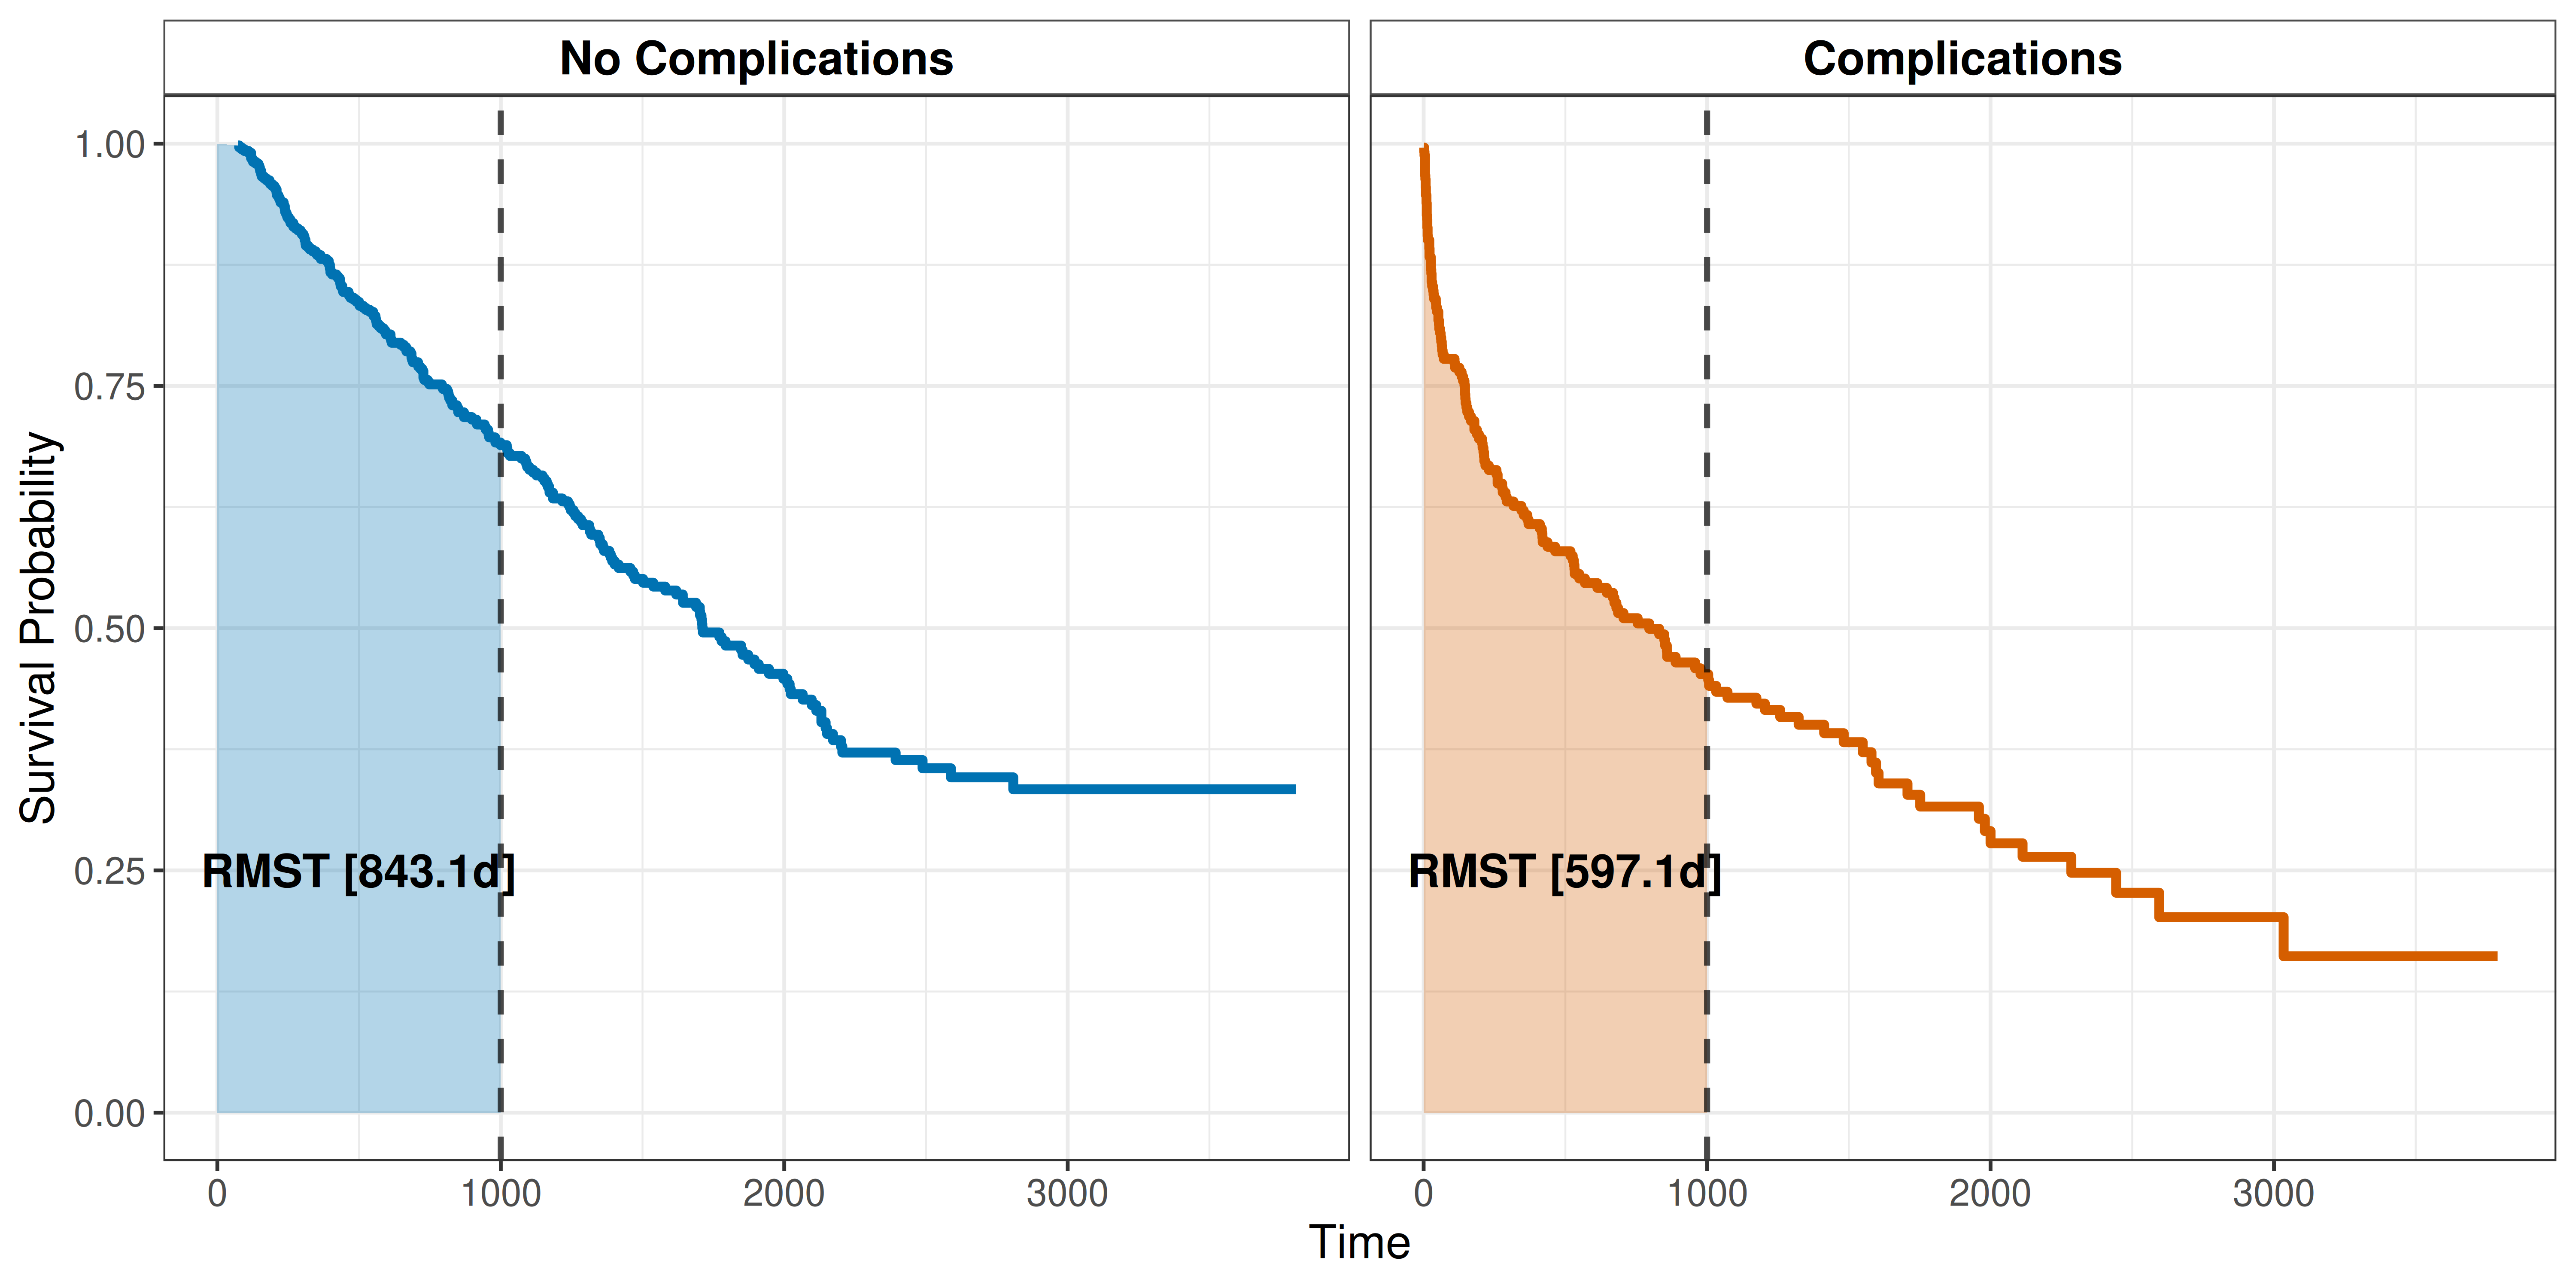
\includegraphics[width=0.9\linewidth,height=\textheight,keepaspectratio]{Figures/reductions/fig-p4c21-pseudo-rmst.png}

}

\caption{\label{fig-p4c21-pseudo-rmst}Survival curves with RMST
visualization at \(\tau = 1000\) days, stratified by complications
status. The shaded area under each curve represents the RMST, with the
numerical value displayed as text.}

\end{figure}%

To compare the RMST estimates to the pseudo-value approach, fit the
linear model

\[
\widehat{\operatorname{RMST}}(\tau \mid \mathbf{x}_i) = \hat{\tilde{y}}_i(\tau) = \hat{\beta}_{\tau,0} + \hat{\beta}_{\tau,1} x_{i,1},\quad x_{i,1} = \mathbb{I}(\text{complications}_i = \text{`yes'}),
\]

again assuming the identity function for the response.

For time point \(\tau = 1000\) days, the estimated coefficient is
\(\hat{\beta}_{1000,1} \approx -239\). Thus, the expected RMST for
patients with complications is reduced by around 239 days, which is
close to the result obtained from the Kaplan-Meier analysis in
Figure~\ref{fig-p4c21-pseudo-rmst}. Once again, this model can be
extended to include age such that

\[
\widehat{\operatorname{RMST}}(\tau \mid \mathbf{x}_i) = \hat{\beta}_{\tau,0} + \hat{\beta}_{\tau,1} x_{i,1} + \hat{\beta}_{\tau,2} x_{i,2},\quad x_{i,1} = \mathbb{I}(\text{complications}_i = \text{`yes'}), x_{i,2} = \text{age}_i,
\]

where \(x_{i,1}\) as before and \(x_{i,2}\) is the age of subject \(i\).
The respective estimates are \(\hat{\beta}_{1000,1} \approx -230\) and
\(\hat{\beta}_{1000,2} \approx -3\), such that, holding the other
covariates fixed, the expected RMST is reduced by around 3 days per year
of age. The effect of complications, \(\hat{\beta}_{1000,1}\), is
slightly reduced when age is included and can be interpreted as the
effect of complications on RMST adjusted for age.

\section{Choice of response
function}\label{sec-pseudo-value-response-function}

The examples in Section~\ref{sec-pseudo-value-S} and
Section~\ref{sec-pseudo-value-rmst} assumed the identity response for
simplicity.\index{response function} In general, the response function
\(r(\cdot)\) in (\ref{eq-pseudo-value-response-function}) is a modeling
choice with two distinct but related consequences: how the model is
estimated, and how covariate effects are interpreted.

\subsection{Post-hoc vs.~embedded
applications}\label{post-hoc-vs.-embedded-applications}

The simplest approach is to apply \(r(\cdot)\) post-hoc, meaning a
regression model is fit on the raw pseudo-values (for example,
minimizing squared error) and then the predictions are transformed. This
is straightforward and works with any off-the-shelf regression method,
but the optimization objective no longer corresponds to the final target
space. For example, when \(r(\cdot)\) is the sigmoid, a model trained
with squared error on pseudo-values \(\tilde{y}_i \in \mathbb{R}\) will
not necessarily minimize the error of the final probabilities
\(r(\hat\eta(\mathbf{x})) \in [0,1]\).

The alternative is to embed \(r(\cdot)\) into the fitting process by
modifying the loss function. This works particularly well for models
that support custom loss functions, such as gradient boosting machines
(Chapter~\ref{sec-boost}) and neural networks (Chapter~\ref{sec-nnet}).
For example, when the target is a survival probability, one can use the
log loss (Chapter~\ref{sec-rules}), \[
\ell(\tilde{y}_i, \eta(\mathbf{x}_i\mid\boldsymbol{\theta}_\tau)) = -\left[\tilde{y}_i \log r(\eta(\mathbf{x}_i\mid\boldsymbol{\theta}_\tau)) + (1 - \tilde{y}_i) \log(1 - r(\eta(\mathbf{x}_i\mid\boldsymbol{\theta}_\tau)))\right],
\]

where \(r(\cdot)\) is the sigmoid function and
\(\eta(\mathbf{x}_i\mid\boldsymbol{\theta}_\tau)\) is the model output
on the logit scale (Table~\ref{tbl-pseudo-link-interpretation}). This
approach ensures the gradient updates during training are consistent
with the final probability scale, which can improve calibration and
estimation (Hothorn 2021). For RMST targets, which take values in
\([0, \tau]\), the exponential response is a natural choice to guarantee
positive fitted values. Using this response function yields coefficients
interpretable as log-RMST ratios (Andersen, Hansen, and Klein 2004;
Sachs and Gabriel 2022).

Although alternative response functions are available, the identity
response (or a post-hoc transformation) is often sufficient in practice
and may be preferred for its simplicity, particularly when only
predictive performance is of interest. This works best when \(\tau\) is
not too close to the start or end of follow-up, as the pseudo-values
then stay away from the boundary of the target space (for example, near
\(0\) or \(1\) when estimating probabilities). This was seen in
Figure~\ref{fig-p4c21-pseudo-lm}, where the predictions remained within
the required \([0,1]\) range despite the use of the identity response
function.

\subsection{Interpretation of covariate
effects}\label{interpretation-of-covariate-effects}

The response function determines how estimated feature effects should be
interpreted. Table~\ref{tbl-pseudo-link-interpretation} summarizes the
most common choices when estimating survival probabilities, along with
their interpretations after the response function is applied; all assume
a linear predictor \(\hat\eta\), with estimated coefficients
\(\hat{\boldsymbol{\beta}}_\tau\).

\begin{longtable}[]{@{}
  >{\raggedright\arraybackslash}p{(\linewidth - 4\tabcolsep) * \real{0.3333}}
  >{\raggedright\arraybackslash}p{(\linewidth - 4\tabcolsep) * \real{0.3333}}
  >{\raggedright\arraybackslash}p{(\linewidth - 4\tabcolsep) * \real{0.3333}}@{}}
\caption{Common response functions for pseudo-value regression on
estimated survival probability targets
(\(\hat{\psi} = \hat{S}(\tau \mid \mathbf{x})\)) and the associated
interpretation of their corresponding covariate
effects.}\label{tbl-pseudo-link-interpretation}\tabularnewline
\toprule\noalign{}
\begin{minipage}[b]{\linewidth}\raggedright
Link \(r^{-1}(\hat{\psi})\)
\end{minipage} & \begin{minipage}[b]{\linewidth}\raggedright
Response \(r(\hat\eta(\mathbf{x}))\)
\end{minipage} & \begin{minipage}[b]{\linewidth}\raggedright
Interpretation of \(\hat{\beta}_{\tau,j}\)
\end{minipage} \\
\midrule\noalign{}
\endfirsthead
\toprule\noalign{}
\begin{minipage}[b]{\linewidth}\raggedright
Link \(r^{-1}(\hat{\psi})\)
\end{minipage} & \begin{minipage}[b]{\linewidth}\raggedright
Response \(r(\hat\eta(\mathbf{x}))\)
\end{minipage} & \begin{minipage}[b]{\linewidth}\raggedright
Interpretation of \(\hat{\beta}_{\tau,j}\)
\end{minipage} \\
\midrule\noalign{}
\endhead
\bottomrule\noalign{}
\endlastfoot
Identity\(\hat{\psi}\) & Identity\(\hat\eta(\mathbf{x})\) & Absolute
difference in \(\hat{\psi}(\tau\mid\mathbf{x})\) per unit increase in
\(x_j\) \\
Logit\(\log\frac{\hat{\psi}}{1-\hat{\psi}}\) &
Sigmoid\(\left[1+\exp(-\hat\eta(\mathbf{x}))\right]^{-1}\) & Log-odds
ratio; \(e^{\hat{\beta}_{\tau,j}}\) is an odds ratio \\
Complementary log-log\(\log(-\log(\hat{\psi}))\) & Complementary log-log
inverse\(\exp(-\exp(\hat\eta(\mathbf{x})))\) & Log cumulative hazard
ratio; \(e^{\hat{\beta}_{\tau,j}}\) is a cumulative hazard ratio \\
Log\(\log(\hat{\psi})\) & Exponential\(\exp(\hat\eta(\mathbf{x}))\) &
Log survival ratio; \(e^{\hat{\beta}_{\tau,j}}\) is a survival ratio \\
\end{longtable}

A particular link function to note is the complementary log-log
link.\index{complementary log-log} For survival probability
\(\hat{S}(\tau \mid \mathbf{x})\), applying the complementary log-log
link gives

\begin{equation}\phantomsection\label{eq-cloglog-ph}{
\begin{aligned}
\hat\eta(\mathbf{x})
&= \log\left(-\log(\hat{S}(\tau \mid \mathbf{x}))\right) \\
&= \log\left(\hat{H}(\tau \mid \mathbf{x})\right) \\
&= \log\left(\hat{H}_0(\tau)\exp(\mathbf{x}^\top\hat{\boldsymbol{\beta}}_\tau)\right) \\
&= \log\left(\hat{H}_0(\tau)\right) + \mathbf{x}^\top\hat{\boldsymbol{\beta}}_\tau,
\end{aligned}
}\end{equation}

where the second equality follows from the usual relationships between
the survival and cumulative hazard functions (\ref{eq-surv-haz}), and
the third follows by parameterizing \(\hat{H}(\tau \mid \mathbf{x})\)
using a proportional-hazards-type form with baseline cumulative hazard
\(\hat{H}_0(\tau)\). If the estimated coefficients were equal at all
time points,
\(\hat{\boldsymbol{\beta}}_\tau = \hat{\boldsymbol{\beta}}, \forall \tau\),
then (\ref{eq-cloglog-ph}) recovers the proportional hazards form
(\ref{eq-ph-cum}) and \(\exp(\hat{\beta}_j)\) can be interpreted as a
hazard ratio for feature \(j\).\index{proportional hazards} Therefore,
(\ref{eq-cloglog-ph}) provides a convenient way to investigate the
proportional hazards assumption: substantial variation in
\(\hat{\boldsymbol{\beta}}_\tau\) across \(\tau\) suggests a violation
of proportional hazards (Andersen and Pohar Perme 2010). The form in
(\ref{eq-cloglog-ph}) demonstrates how the pseudo-value framework
generalizes the proportional hazards formulation by allowing departures
from proportionality through time-varying
effects.\index{time-varying effects}

For RMST targets, the identity link yields coefficients directly
interpretable as differences in expected survival time (for example,
days), whereas the log link gives log-RMST-ratios (Royston and Parmar
2011b). The former is more common in practice due to its direct clinical
interpretability (Tian, Zhao, and Wei 2014).

\section{Pseudo-values in event history
analysis}\label{sec-pseudo-value-eha}

The pseudo-value approach can be extended to more complex event history
settings, including competing risks and multi-state models (Andersen,
Klein, and Rosthøj 2003; Andersen and Pohar Perme 2010; Parner,
Andersen, and Overgaard 2023). The key idea remains the same: use
univariate, non-parametric estimators of the quantity of interest to
calculate pseudo-values, which can then be used as target variables in
regression models.

\subsection{Pseudo-values for competing
risks}\label{sec-pseudo-value-cr}

In the competing risks setting (Section~\ref{sec-competing-risks}), a
quantity of particular interest is the cumulative incidence function
(CIF)
\(F_q(\tau)\).\index{reduction!pseudo-value regression!competing risks}\index{competing risks}
A consistent estimator for the CIF is the Aalen-Johansen estimator
(Section~\ref{sec-aalen-johansen}) and pseudo-values for the CIF are
thus given by:

\[
\tilde{y}_{i,q}(\tau) = n\hat{F}_{AJ,q}(\tau) - (n-1)\hat{F}_{AJ,q}^{-i}(\tau),
\]

where \(\hat{F}_{AJ,q}^{-i}(\tau)\) is the Aalen-Johansen estimate of
the CIF for event type \(q\) obtained by omitting the \(i\)th
observation from the dataset.

Once calculated, these pseudo-values can be used as target variables in
regression models to estimate the conditional CIF,
\(F_q(\tau \mid \mathbf{x}_i)\), via
(\ref{eq-pseudo-value-expectation-2}). Using the identity function for
the response, one can directly interpret the feature effects on the
cumulative incidence of a specific event type.

\subsection{Pseudo-values for multi-state
models}\label{sec-pseudo-value-occupation-prob}

In multi-state settings (Section~\ref{sec-multi-state}), pseudo-values
can be used to estimate state occupation probabilities conditional on
features.\index{reduction!pseudo-value regression!multi-state models}
These represent the probability of being in state \(q\) at time
\(\tau\). Non-parametric estimators for state occupation probabilities
can be obtained via the Aalen-Johansen estimator for multi-state models
(Section~\ref{sec-ms-state-occupation}). The pseudo-values for state
occupation probabilities are then defined as:

\[
\tilde{y}_{i,q}(\tau) = n\hat{P}_{AJ,q}(\tau) - (n-1)\hat{P}_{AJ,q}^{-i}(\tau),
\]

where \(\hat{P}_{AJ,q}(\tau)\) is the Aalen-Johansen estimate of the
state occupation probability for state \(q\) at time \(\tau\), and
\(\hat{P}_{AJ,q}^{-i}(\tau)\) is the same estimate obtained by omitting
the \(i\)th observation.

These pseudo-values can be used to model conditional state occupation
probabilities \(P_q(\tau \mid \mathbf{x}_i)\) using standard regression
techniques. This approach is particularly flexible as it allows for
modeling state occupation probabilities directly, without the need to
specify and estimate all transition hazards (Andersen, Klein, and
Rosthøj 2003).

\section{Conclusion}\label{conclusion-14}

\begin{tcolorbox}[enhanced jigsaw, toprule=.15mm, bottomtitle=1mm, opacityback=0, breakable, leftrule=.75mm, title={Key takeaways}, toptitle=1mm, bottomrule=.15mm, colback=white, colframe=quarto-callout-warning-color-frame, titlerule=0mm, opacitybacktitle=0.6, coltitle=black, rightrule=.15mm, left=2mm, colbacktitle=quarto-callout-warning-color!10!white, arc=.35mm]

\begin{itemize}
\tightlist
\item
  The pseudo-value regression reduction estimates quantities of interest
  at specific time points conditional on covariates by transforming
  censored survival outcomes into regression targets derived from
  univariate estimators.
\item
  The approach avoids strong assumptions such as proportional hazards
  and accelerated failure time, naturally accommodates time-varying
  effects, and extends to competing risks and multi-state settings.
\item
  When the identity response is used, feature effects are directly
  interpretable on the scale of the target quantity, and standard
  survival analysis metrics can be used for model evaluation.
\item
  Pseudo-values are not independent, can fall outside the natural range
  of the target quantity, and may be computationally expensive to
  calculate for many time points, although response functions and
  efficient approximations can mitigate these limitations.
\end{itemize}

\end{tcolorbox}

\begin{tcolorbox}[enhanced jigsaw, toprule=.15mm, bottomtitle=1mm, opacityback=0, breakable, leftrule=.75mm, title={Further reading}, toptitle=1mm, bottomrule=.15mm, colback=white, colframe=quarto-callout-tip-color-frame, titlerule=0mm, opacitybacktitle=0.6, coltitle=black, rightrule=.15mm, left=2mm, colbacktitle=quarto-callout-tip-color!10!white, arc=.35mm]

\begin{itemize}
\tightlist
\item
  Andersen, Klein, and Rosthøj (2003) is the foundational paper
  introducing pseudo-value regression via generalized estimating
  equations, with applications to multi-state models.
\item
  Andersen, Hansen, and Klein (2004) extends the pseudo-value approach
  to RMST targets.
\item
  Andersen and Pohar Perme (2010) provides a comprehensive overview of
  pseudo-value methods in survival analysis.
\item
  Parner, Andersen, and Overgaard (2023) and Bouaziz (2023) specifically
  discuss pseudo-value calculations in the context of different
  censoring types.
\item
  Sachs and Gabriel (2022) describe computational approaches and provide
  an implementation in the R package \texttt{eventglm}.
\item
  Ulla B. Mogensen and Gerds (2013) extend the pseudo-value idea to
  random forests in the competing risks setting.
\item
  Lili Zhao and Feng (2020b) and Schenk, Basten, and Schmid (2025)
  illustrate how pseudo-values can be used as targets for deep neural
  networks and random forests, respectively.
\end{itemize}

\end{tcolorbox}

\chapter{Partition-Based
Reductions}\label{sec-partition-based-reductions}

In contrast to the previously introduced reductions that focus on the
estimation of a specific quantity of interest at one or a few time
points, partition-based reductions aim to estimate the entire
distribution of the event times.\index{reduction!partition reductions}
The general idea is to partition the time axis into \(J\) disjoint
intervals \([a_0,a_1),\ldots,[a_{J-1},a_J)\) and estimate a discrete or
continuous hazard rate for each interval. Intervals do not need to be of
the same size.

For illustration, consider the partitioning of the follow-up in
Figure~\ref{fig-p4c22-fu-partitioning}. Let \(I_j:=[a_{j-1},a_{j})\) be
the \(j\)th interval and let \(J_i\) denote the index of the interval in
which the observed time \(t_i\) of subject \(i\) falls, that is
\(t_i \in I_{J_i} = [a_{J_i-1},a_{J_i})\).

\begin{figure}

\centering{

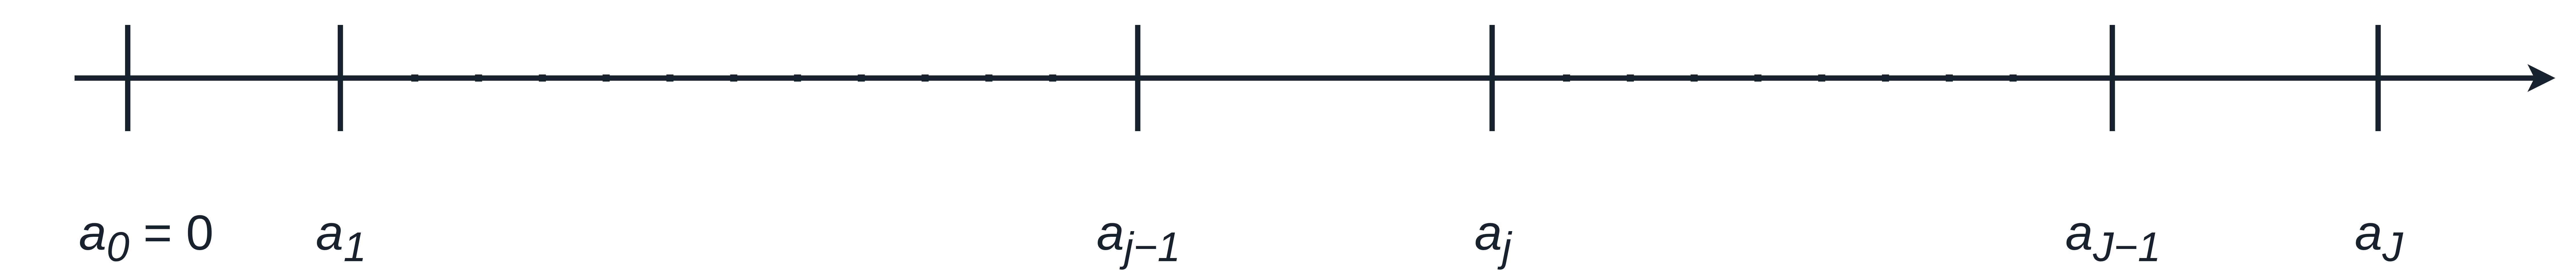
\includegraphics[width=0.9\linewidth,height=\textheight,keepaspectratio]{Figures/reductions/fig-p4c22-fu-partitioning.png}

}

\caption{\label{fig-p4c22-fu-partitioning}Partitioning of the follow-up
time into \(J\) discrete intervals \([a_0,a_1), \ldots, [a_{J-1},a_J)\).
This partitioning forms the basis for the reduction techniques discussed
in this chapter.}

\end{figure}%

Formally, define the partitioning of the follow-up times via the set of
interval boundary points \(\{a_{j-1}, a_j\}\) for \(j=1,\ldots,J\) as:

\begin{equation}\phantomsection\label{eq-cut-points}{
\mathcal{A} = \{a_0, a_1, \ldots, a_J\}, \quad a_0 < a_1 < \ldots < a_J,
}\end{equation}

where \(a_0\) will often be zero and \(a_J\) some time point larger than
the last observed follow-up time. This partitioning is used to create a
transformed dataset, based on which standard regression or
classification methods can be used to estimate (discrete) hazards in
each interval. Section~\ref{sec-data-transformation} introduces the
required data transformation in more detail. Then
Section~\ref{sec-discrete-time-reduction},
Section~\ref{sec-survival-stacking} and
Section~\ref{sec-piecewise-constant-hazards} define specific reductions
based on this data transformation, including theoretical justifications
and illustrative examples. Finally,
Section~\ref{sec-choice-of-interval-boundaries} discusses computational
aspects and modeling choices, including the choice of interval
boundaries \(a_j\) and the convention for left-closed versus left-open
intervals.

\section{Data transformation}\label{sec-data-transformation}

In order to apply the reduction techniques introduced in the upcoming
sections, standard time-to-event data needs to be transformed into a
specific format. The transformation is based on the partitioning of the
follow-up as illustrated in Figure~\ref{fig-p4c22-fu-partitioning} and
the interval boundaries defined in (\ref{eq-cut-points}).
Figure~\ref{fig-p4c22-data-trafo} illustrates the resulting structure
for three hypothetical subjects and interval boundaries
\(\mathcal{A} = \{0, 1.5, 3\}\). The left-hand side shows the original
time-to-event format (one row per subject), the right-hand side shows
the transformed dataset \(\mathcal{D}_{\mathcal{A}}\) that the rest of
this section formalizes (all notation will also be defined).

\begin{figure}

\centering{

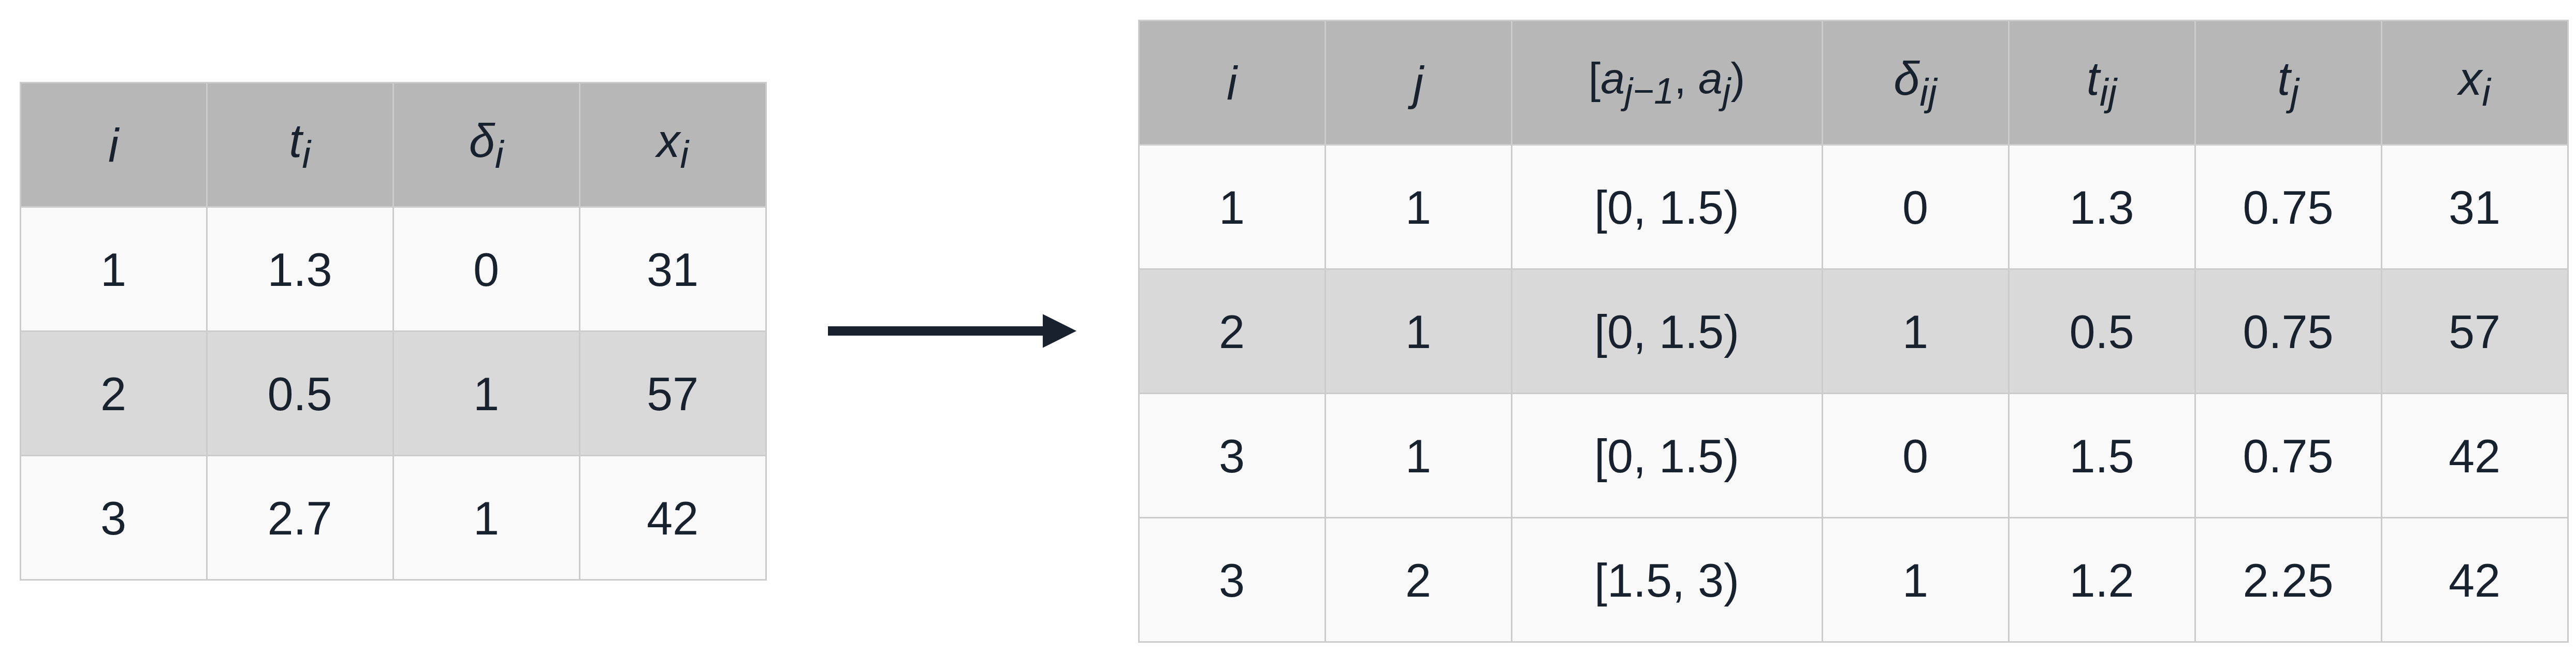
\includegraphics[width=1\linewidth,height=\textheight,keepaspectratio]{Figures/reductions/fig-p4c22-data-trafo-pem.png}

}

\caption{\label{fig-p4c22-data-trafo}Illustration of the data
transformation needed for partition-based reductions. Left: Data in
standard time-to-event format. Right: Transformed data using interval
boundaries \(\mathcal{A} = \{0, 1.5, 3\}\).}

\end{figure}%

The new dataset contains \(J_i\) rows for each subject \(i\), that is
one row for each interval in which subject \(i\) was at risk of
experiencing an event. For each subject \(i\), their interval-specific
event indicator is given by:

\begin{equation}\phantomsection\label{eq-interval-indicator}{
\delta_{ij} = \begin{cases}
1, & t_i \in [a_{j-1}, a_j) \wedge \delta_i = 1, \\
0, & \text{otherwise},
\end{cases}\quad j=1,\ldots,J_i,
}\end{equation}

with \(\delta_{ij}=0\) for all intervals except the last interval of
subject \(i\), where \(\delta_{iJ_i} = \delta_i\). Thus, the total
number of events is unchanged by the transformation, and given
\(\mathcal{A}\), the values \(\delta_{ij}\) are determined entirely by
the original data.

Further, let \(t_{ij}\) be the time that subject \(i\) was at risk for
the event in interval \(j\),

\begin{equation}\phantomsection\label{eq-time-at-risk}{
t_{ij} = \begin{cases}
a_j - a_{j-1}, & \text{ if } t_i > a_j, \\
t_i - a_{j-1}, & \text{ otherwise,}\\
\end{cases}\quad j=1,\ldots,J_i,
}\end{equation}

or in words, if \(i\) experienced the event or was censored in interval
\(j\) then \(t_{ij}\) is the time taken within that interval until the
outcome occurred, otherwise, \(t_{ij}\) is simply the interval length.
Let further \(t_j\) be a continuous representation of the time axis, one
common choice being the interval midpoint

\[
t_j = \frac{a_{j-1} + a_j}{2}.
\]

The transformation is completed by recording the subject's (potentially
time-dependent) features \(\mathbf{x}_{ij}\) with
\(\mathbf{x}_{ij} = \mathbf{x}_{i}\) for all \(j\) if features are
constant over time.

Thus, given the partition \(\mathcal{A}\), the standard time-to-event
data \(\mathcal{D}= \{(t_i, \delta_i, \mathbf{x}_i)\}_{i=1,\ldots,n}\)
is transformed to the dataset (Figure~\ref{fig-p4c22-data-trafo}),

\[
\mathcal{D}_{\mathcal{A}} = \{(i, j, \delta_{ij}, \mathbf{x}_{ij}, t_{ij}, t_j)\}_{i=1,\ldots,n;\  j=1,\ldots,J_i},
\]

where \(i\) and \(j\) are indices not used in modeling and \(t_{ij}\) is
only required for the piecewise constant hazards approach
(Section~\ref{sec-piecewise-constant-hazards}). \(t_j\) is the only
feature that is shared across all subjects within an interval and is
used to estimate the baseline hazard; in many software implementations,
it is included as another column of \(\mathbf{x}_{ij}\), though it is
kept separate in this chapter to emphasize its role.

\section{Discrete-time survival
analysis}\label{sec-discrete-time-reduction}

Recall from Section~\ref{sec-distributions-discrete} that \(\tilde{Y}\)
denotes \emph{discretized} time, such that
\(\tilde{Y}=j \Leftrightarrow Y \in [a_{j-1}, a_j)\).\index{discrete-time survival analysis}\index{reduction!partition reductions!discrete-time}
Now consider the partitioning of the follow-up (\ref{eq-cut-points}),
assuming interest is only in whether the event occurred within an
interval rather than the exact event time. The likelihood contribution
of the \(i\)th observation is given by
\(\Pr(Y_i \in [a_{J_i-1}, a_{J_i})) = \Pr(\tilde{Y}_i = J_i)\) for
subjects who experienced an event (\(\delta_i = 1\)) and
\(\Pr(Y_i \geq a_{J_i}) = \Pr(\tilde{Y}_i > J_i)\) for censored
observations (\(\delta_i = 0\)).

Recall also from Section~\ref{sec-distributions-discrete} the
discrete-time survival and event-probability identities,
\begin{equation}\phantomsection\label{eq-discrete-survival}{
S_{\tilde{Y}}(j) = \prod_{k \leq j}(1 - h_{\tilde{Y}}(k)) \quad\text{and}\quad \Pr(\tilde{Y} = j) = S_{\tilde{Y}}(j-1)\, h_{\tilde{Y}}(j).
}\end{equation}

Applying these to the likelihood contribution of subject \(i\), and
using the interval-specific event indicators \(\delta_{ij}\) from
(\ref{eq-interval-indicator}) (in particular
\(\delta_{iJ_i} = \delta_i\) and \(\delta_{ij}=0\) for \(j<J_i\)), gives

\begin{equation}\phantomsection\label{eq-discrete-likelihood}{\begin{aligned}
L_i
&= \Pr(Y_i \in [a_{J_i-1}, a_{J_i}))^{\delta_i}\, \Pr(Y_i \geq a_{J_i})^{1-\delta_i}\\
&= \left[S_{\tilde{Y}}(J_i-1)\, h_{\tilde{Y}}(J_i)\right]^{\delta_i} \left[S_{\tilde{Y}}(J_i)\right]^{1-\delta_i}\\
&= \left[\prod_{j=1}^{J_i-1} (1-h_{\tilde{Y}}(j)) \cdot h_{\tilde{Y}}(J_i)\right]^{\delta_i} \left[\prod_{j=1}^{J_i} (1-h_{\tilde{Y}}(j))\right]^{1-\delta_i}\\
&= \prod_{j=1}^{J_i} (1-h_{\tilde{Y}}(j))^{1-\delta_{ij}}\, h_{\tilde{Y}}(j)^{\delta_{ij}}.
\end{aligned}
}\end{equation}

For a random variable \(Z \sim \text{Bernoulli}(\pi)\) with
\(\pi = \Pr(Z = 1)\), the likelihood contribution is
\(\Pr(Z = z) = \pi^z (1-\pi)^{1-z}\), which is exactly the form of each
factor in (\ref{eq-discrete-likelihood}) under the identification
\(\pi = h_{\tilde{Y}}(j)\). The interval-specific event indicators
\(\delta_{ij}\) can therefore be modeled as independent Bernoulli random
variables,

\[
\Delta_{ij} \stackrel{iid}{\sim} \text{Bernoulli}(\pi_j), \quad j = 1, \ldots, J_i,
\]

where the success probability \(\pi_j\) is the discrete-time hazard,

\begin{equation}\phantomsection\label{eq-discrete-hazard-probability}{
\pi_j = \Pr(\Delta_{ij} = 1 \mid t_j) = \Pr(Y_i \in [a_{j-1}, a_j) \mid Y_i \geq a_{j-1}) = h_{\tilde{Y}}(j).
}\end{equation}

This implies that the discrete-time hazards \(h_{\tilde{Y}}(j)\) can be
estimated for each interval \(j\) by fitting any binary classification
model to the transformed dataset

\[
\mathcal{D}_{\mathcal{A}} = \{(\delta_{ij}, t_{j})\}_{i=1,\ldots,n;\quad j=1,\ldots,J_i},
\]

where \(\delta_{ij}\) are the targets and \(t_j\) is a covariate used to
estimate different hazards/probabilities in different intervals.

In the presence of features \(\mathbf{x}_{ij}\), it follows:

\[
\Delta_{ij} \mid \mathbf{x}_{ij}, t_j \stackrel{iid}{\sim} \text{Bernoulli}(\pi_{ij}),
\]

where
\(\pi_{ij} = \Pr(\Delta_{ij} = 1 \mid \mathbf{x}_{ij}, t_j) = h_{\tilde{Y}}(j \mid \mathbf{x}_{ij})\)
is the discrete hazard rate for interval \(j\) given features
\(\mathbf{x}_{ij}\) and is estimated by applying binary classifiers to

\[
\mathcal{D}_{\mathcal{A}} = \{(\delta_{ij}, \mathbf{x}_{ij}, t_{j})\}_{i=1,\ldots,n;\quad j=1,\ldots,J_i}.
\]

To summarize, when fitting a classification model with \(\delta_{ij}\)
as the binary target and \((\mathbf{x}_{ij}, t_j)\) as covariates, the
predicted class probabilities
\(\hat{\pi}_{ij} = \widehat{\Pr}(\Delta_{ij}=1 \mid \mathbf{x}_{ij}, t_j)\)
are estimates of the conditional discrete-time hazard
\(\hat{h}_{\tilde{Y}}(j \mid \mathbf{x}_{ij})\).

To illustrate the discrete-time reduction approach, consider the
\texttt{tumor} dataset introduced in Table~\ref{tbl-surv-data-tumor}.
The follow-up time is partitioned into \(J = 100\) equidistant intervals
and the data are transformed according to the procedure in
Section~\ref{sec-data-transformation}. Define
\(x_{i1} = \mathbb{I}(\text{complications}_i = \text{``yes''})\) and fit
the logistic regression model,

\begin{equation}\phantomsection\label{eq-discrete-time-glm-po}{
\log\frac{\pi_{ij}}{1-\pi_{ij}} = \beta_{0j} + \beta_1 x_{i1},
}\end{equation}

to the transformed dataset, where \(j\) denotes the interval index,
\(\beta_{0j}\) are the interval-specific intercepts and \(\beta_1\) is
the common effect of complications on the discrete hazard rate (across
all intervals).

Predicted discrete hazards are obtained by applying the sigmoid to the
linear predictor: \[
\hat{h}_{\tilde{Y}}(j \mid \mathbf{x}_{ij}) = \hat{\pi}_{ij} = \sigma(\hat{\beta}_{0j} + \hat{\beta}_1 x_{i1}), \qquad \sigma(z) = \frac{1}{1 + \exp(-z)},
\]

where the equality \(\pi_{ij} = h_{\tilde{Y}}(j \mid \mathbf{x}_{ij})\)
was established in (\ref{eq-discrete-hazard-probability}). The estimated
survival probabilities can then be obtained by calculating

\[
\hat{S}_{\tilde{Y}}(j \mid x_{1}) = \prod_{k=1}^j (1-\hat{h}_{\tilde{Y}}(k \mid x_{1})),
\]

for each interval \(j\) and complication group.

Figure~\ref{fig-p4c22-discrete-time-glm} shows the estimated survival
probabilities from the discrete-time model together with the
Kaplan-Meier estimates for comparison, with the model encoded by line
type and complications status by line color. The model specified in
(\ref{eq-discrete-time-glm-po}) is a proportional odds model
(Section~\ref{sec-proportionalodds}), where the baseline hazard is the
same for both complication groups, thus the shape of the hazard and
therefore the survival probability curve is the same for both
complication groups, shifted by the common effect of complications. The
figure indicates that (\ref{eq-discrete-time-glm-po}) does not fit the
data well, as in reality the hazards differ between the two
groups.\index{proportional odds}

\begin{figure}

\centering{

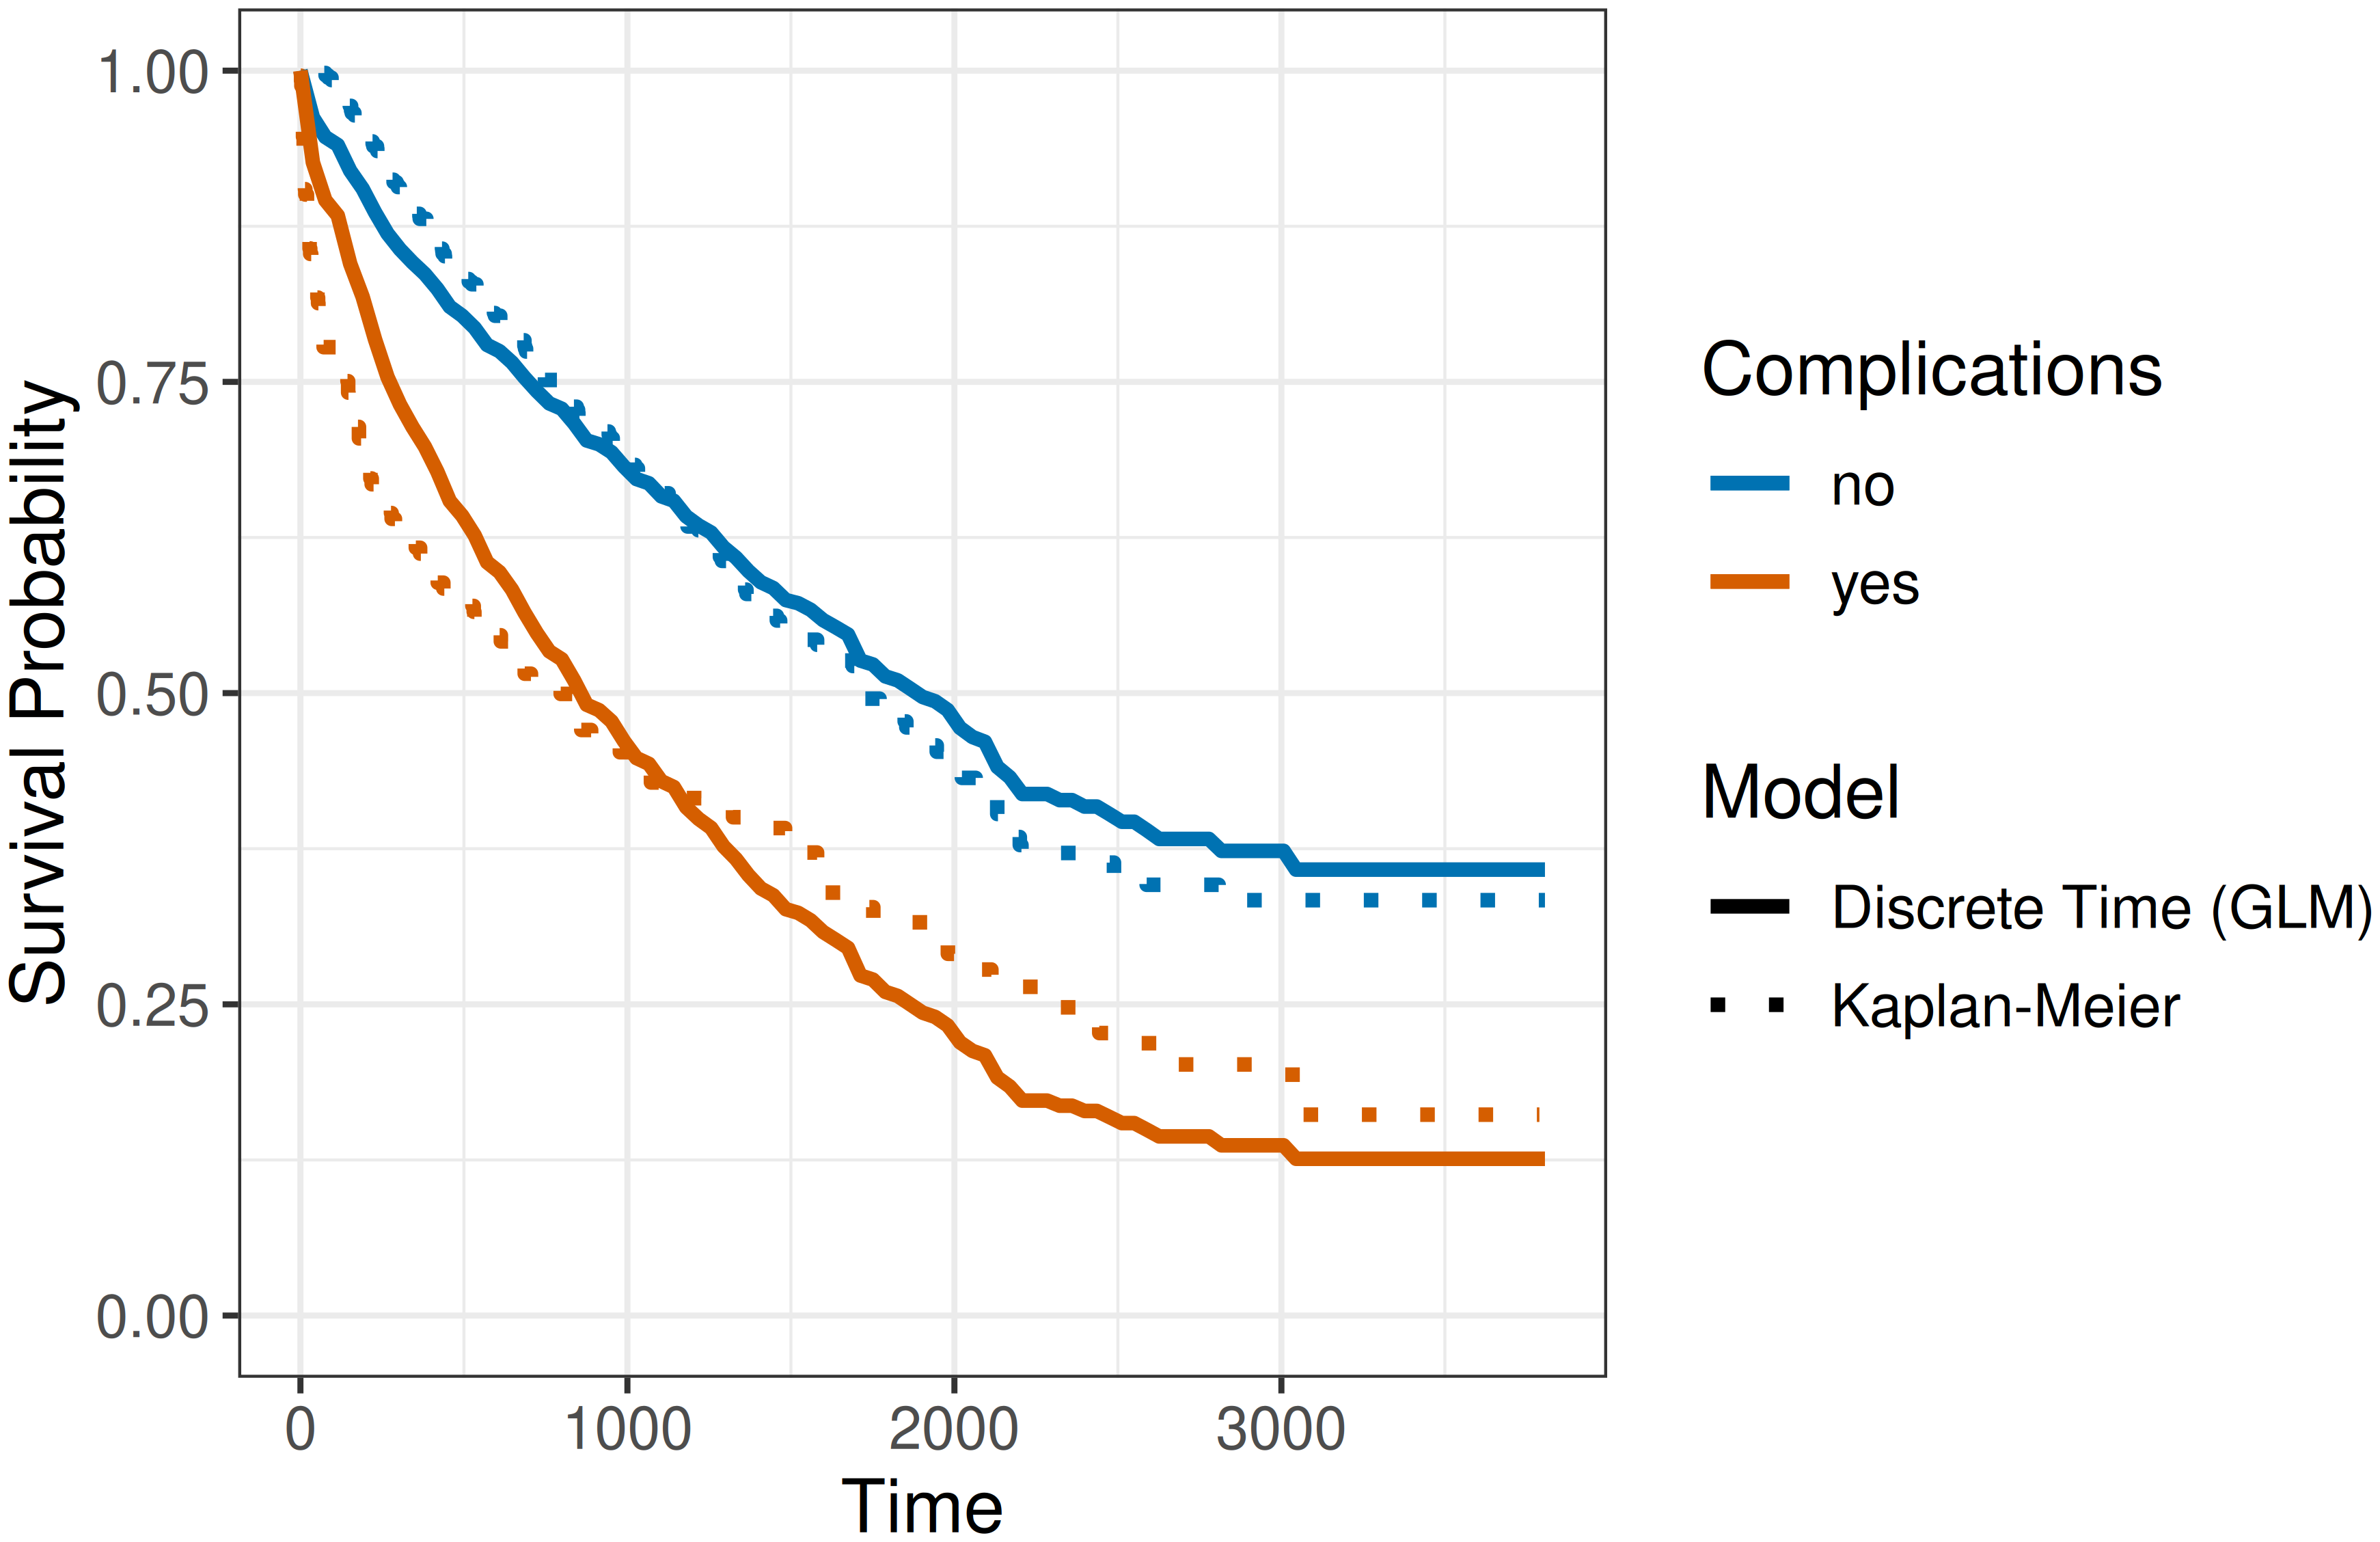
\includegraphics[width=0.7\linewidth,height=\textheight,keepaspectratio]{Figures/reductions/fig-p4c22-discrete-time-glm.png}

}

\caption{\label{fig-p4c22-discrete-time-glm}Comparison of survival
probability estimates using the discrete-time model (logistic
regression) and the Kaplan-Meier estimator, for patients with and
without complications.}

\end{figure}%

To estimate separate discrete baseline hazards for each group,
\(\beta_1\) can be replaced by \(\beta_{1j}\) in
(\ref{eq-discrete-time-glm-po}), which effectively introduces an
interaction term between the interval and complications variables,

\[
\log\frac{\pi_{ij}}{1-\pi_{ij}} = \beta_{0j} + \beta_{1j} x_{i1},
\]

where \(\beta_{0j}\) are the interval-specific intercepts for the
reference group (no complications) and \(\beta_{1j}\) are the deviations
from the reference group for the complications group. This specification
allows the shape of the hazard and therefore the survival probability
curve to differ between the two groups, resulting in a substantially
better fit than the proportional odds model
(Figure~\ref{fig-p4c22-discrete-time-glm-interaction}).

\begin{figure}

\centering{

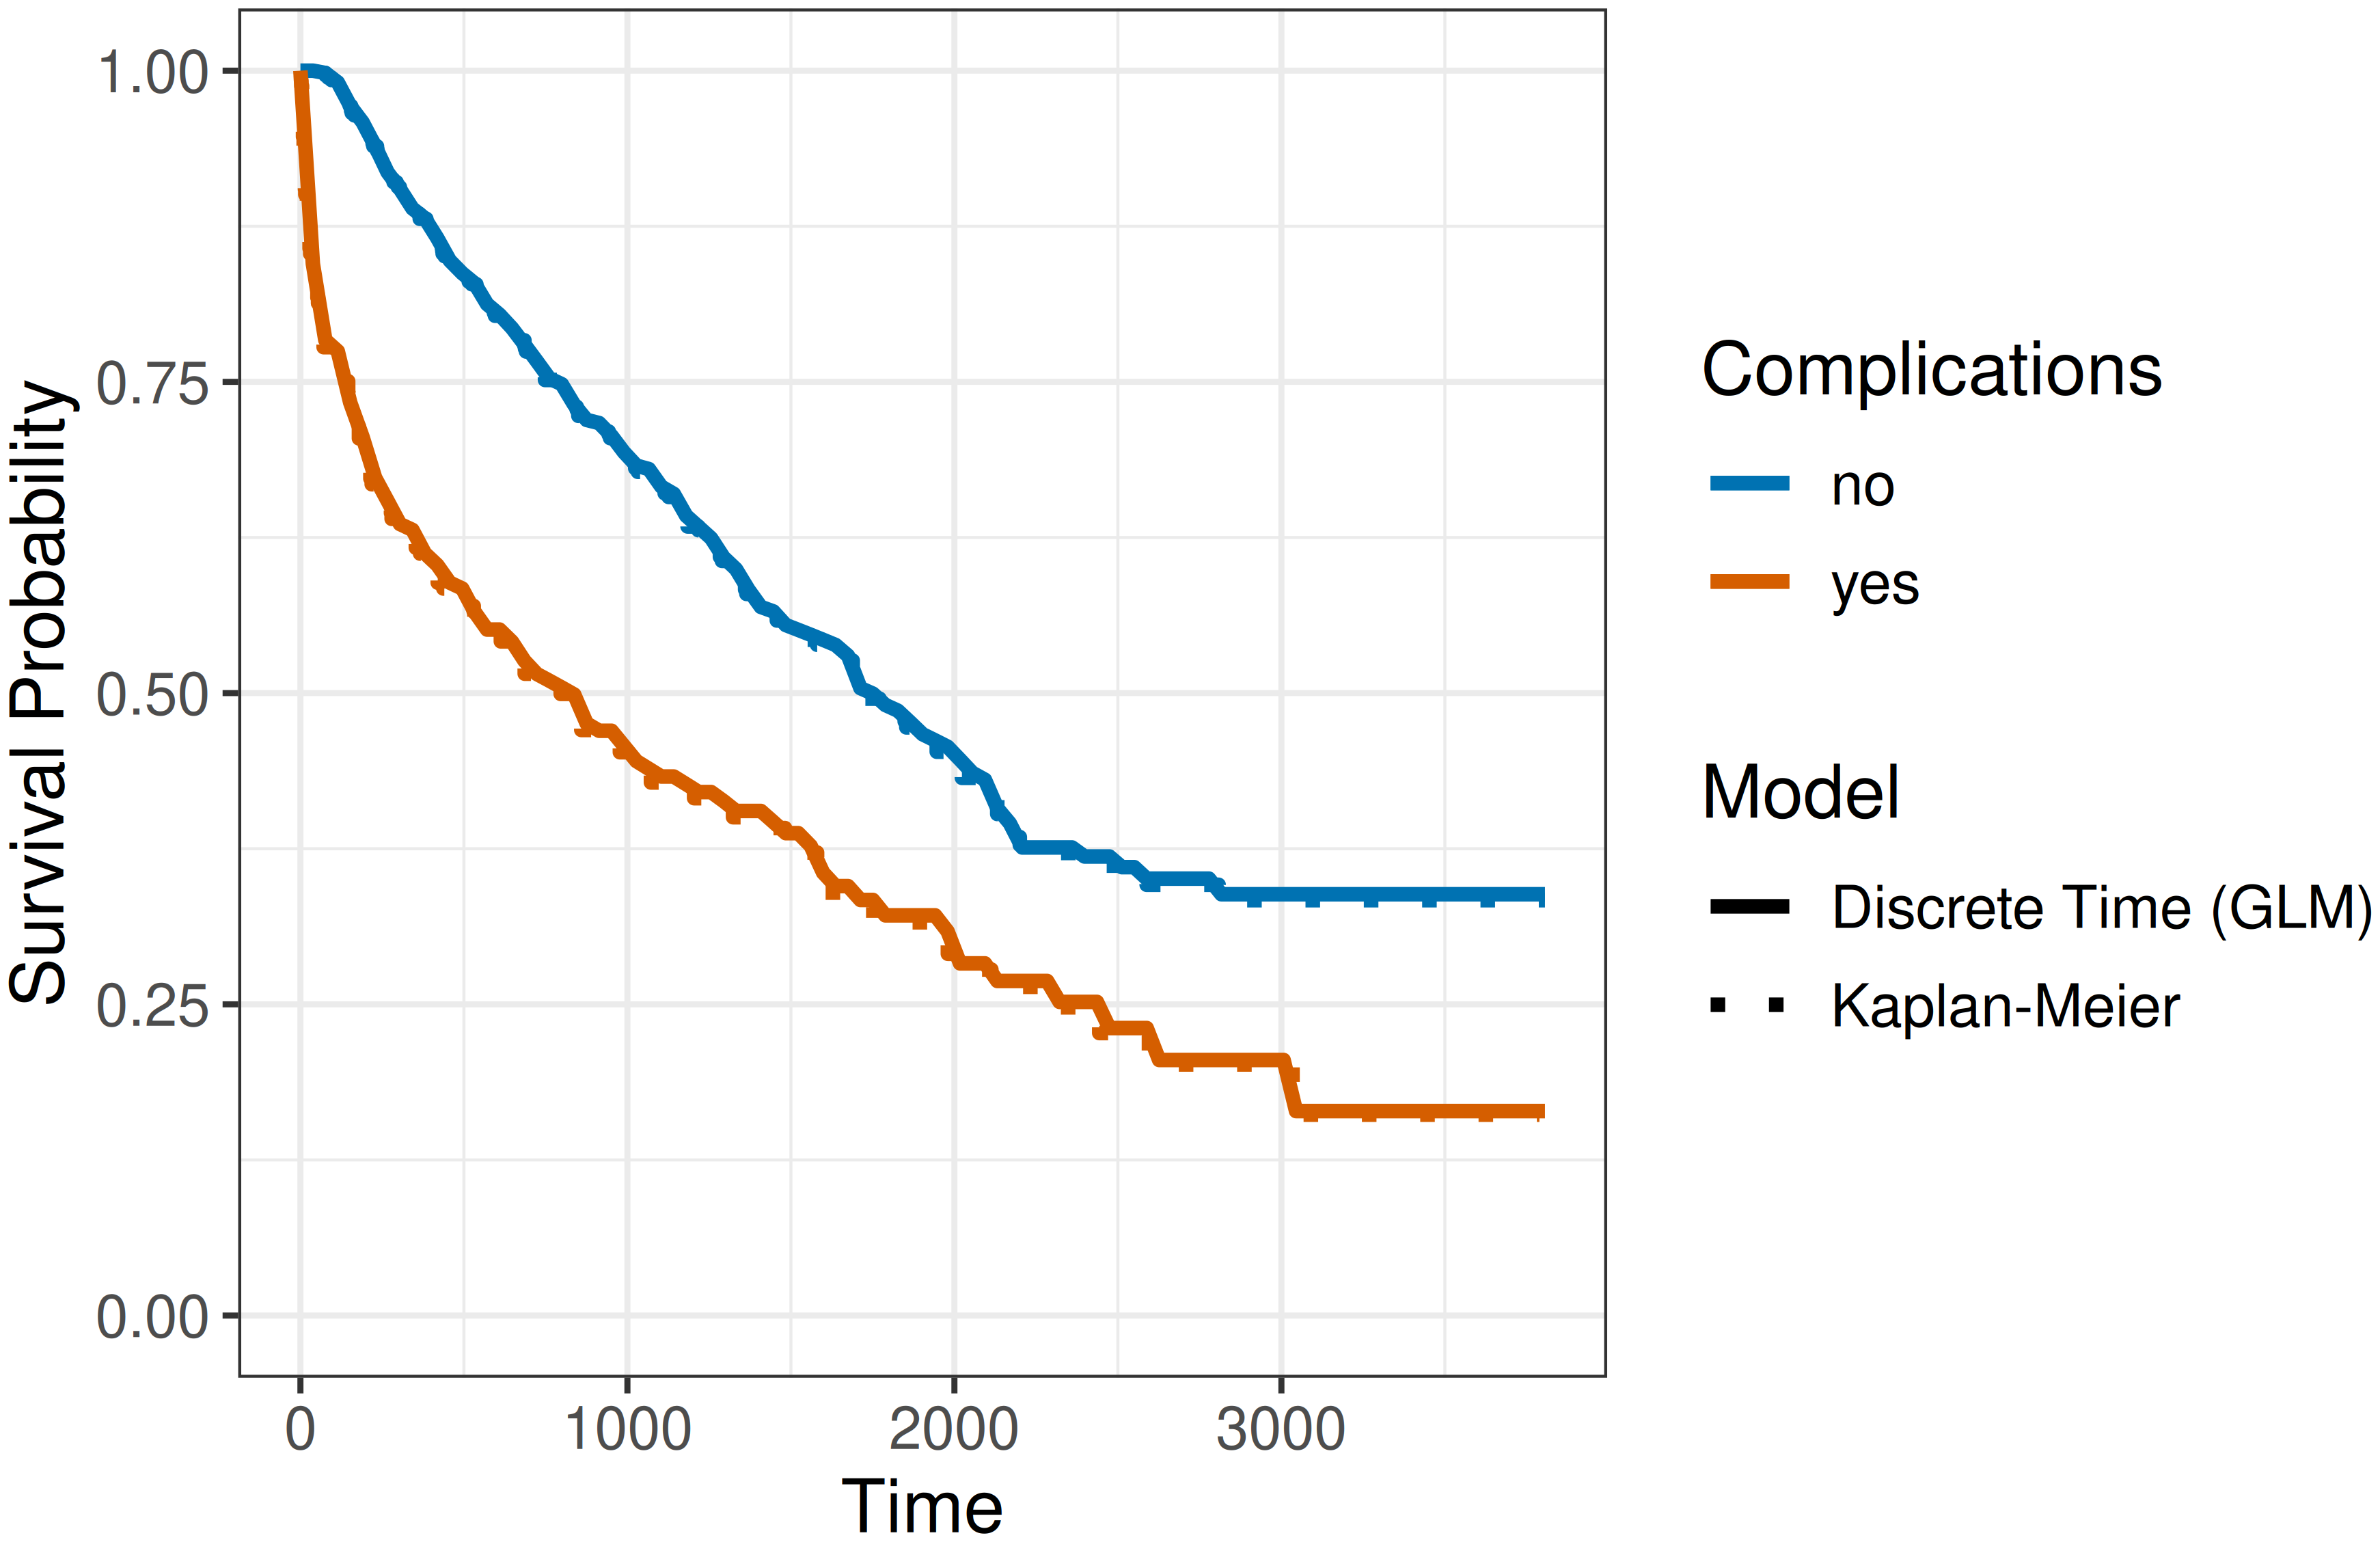
\includegraphics[width=0.7\linewidth,height=\textheight,keepaspectratio]{Figures/reductions/fig-p4c22-discrete-time-glm-interaction.png}

}

\caption{\label{fig-p4c22-discrete-time-glm-interaction}Comparison of
survival probability estimates using the discrete-time model with
interaction (logistic regression) and the Kaplan-Meier estimator, for
patients with and without complications.}

\end{figure}%

While this is a simple example with only one feature, it shows that the
discrete-time reduction approach provides a good approximation of the
event time distribution when the number of intervals is large enough,
even though information about the exact event time was ignored.
Importantly, the estimated survival probabilities are discrete,
representing survival at the interval endpoints. These discrete
estimates can be turned into a continuous survival function using a
variety of approaches, most simply linear interpolation between the
interval endpoints.

The example also raises the question of how to choose the number of
intervals \(J\) and the placement of interval boundaries
\(\mathcal{A}\). These questions will be discussed in more detail in
Section~\ref{sec-choice-of-interval-boundaries}, which is relevant for
both the discrete-time reduction approach and the piecewise constant
hazards approach discussed in
Section~\ref{sec-piecewise-constant-hazards}.

\section{Survival stacking}\label{sec-survival-stacking}

Survival stacking\index{reduction!partition reductions!stacking} (Craig,
Zhong, and Tibshirani 2025) casts survival tasks to classification tasks
similarly to the discrete-time method described in
Section~\ref{sec-discrete-time-reduction}. For estimation purposes, it
is a special case of the discrete-time reduction in which the relevant
time points are the unique observed event times. It connects partition
reductions to Kaplan-Meier and Cox-style estimation, and fixes the
interval boundaries in a data-adaptive way.

Let \(t_{(1)} < t_{(2)} < \ldots < t_{(m)}\) be the unique, observed
event times (as in the construction of the Kaplan-Meier estimator,
Section~\ref{sec-surv-km}), and let
\(\mathcal{R}_{t_{(j)}} = \{i : Y_i \geq t_{(j)}\}\) be the risk set at
\(t_{(j)},\ j=1,\ldots,m\). Survival stacking mirrors the Kaplan-Meier
construction. At each event time it forms an interval
\([t_{(j)}, t_{(j)}+\,\mathrm{d}u)\), where \(\,\mathrm{d}u\) is an
infinitesimally small increment, and records, for every subject in the
risk set, whether the event occurred in that interval,

\[
\delta_{ij} = \begin{cases}
1, & t_i \in [t_{(j)}, t_{(j)}+\,\mathrm{d}u) \wedge \delta_i = 1, \\
0, & \text{otherwise},
\end{cases}\quad i \in \mathcal{R}_{t_{(j)}}.
\]

The construction of the stacked dataset then proceeds exactly as in
Section~\ref{sec-discrete-time-reduction}.

For illustration, consider once again the example from
Figure~\ref{fig-p4c22-data-trafo}. The data transformation for survival
stacking is shown in Figure~\ref{fig-p4c22-data-trafo-stacking} (keeping
only the columns needed for stacking). At the first event time
\(t_{(1)} = 0.5\), all subjects are still at risk for the event. At time
\(t_{(2)} = 2.7\), however, only subject \(3\) is still at risk for the
event. As with Figure~\ref{fig-p4c22-data-trafo}, both transformations
yield four rows in total; however, the discrete-time reduction is more
flexible and will result in fewer intervals per subject when the number
of intervals is smaller than the number of unique event times (\(J<m\)).

\begin{figure}

\centering{

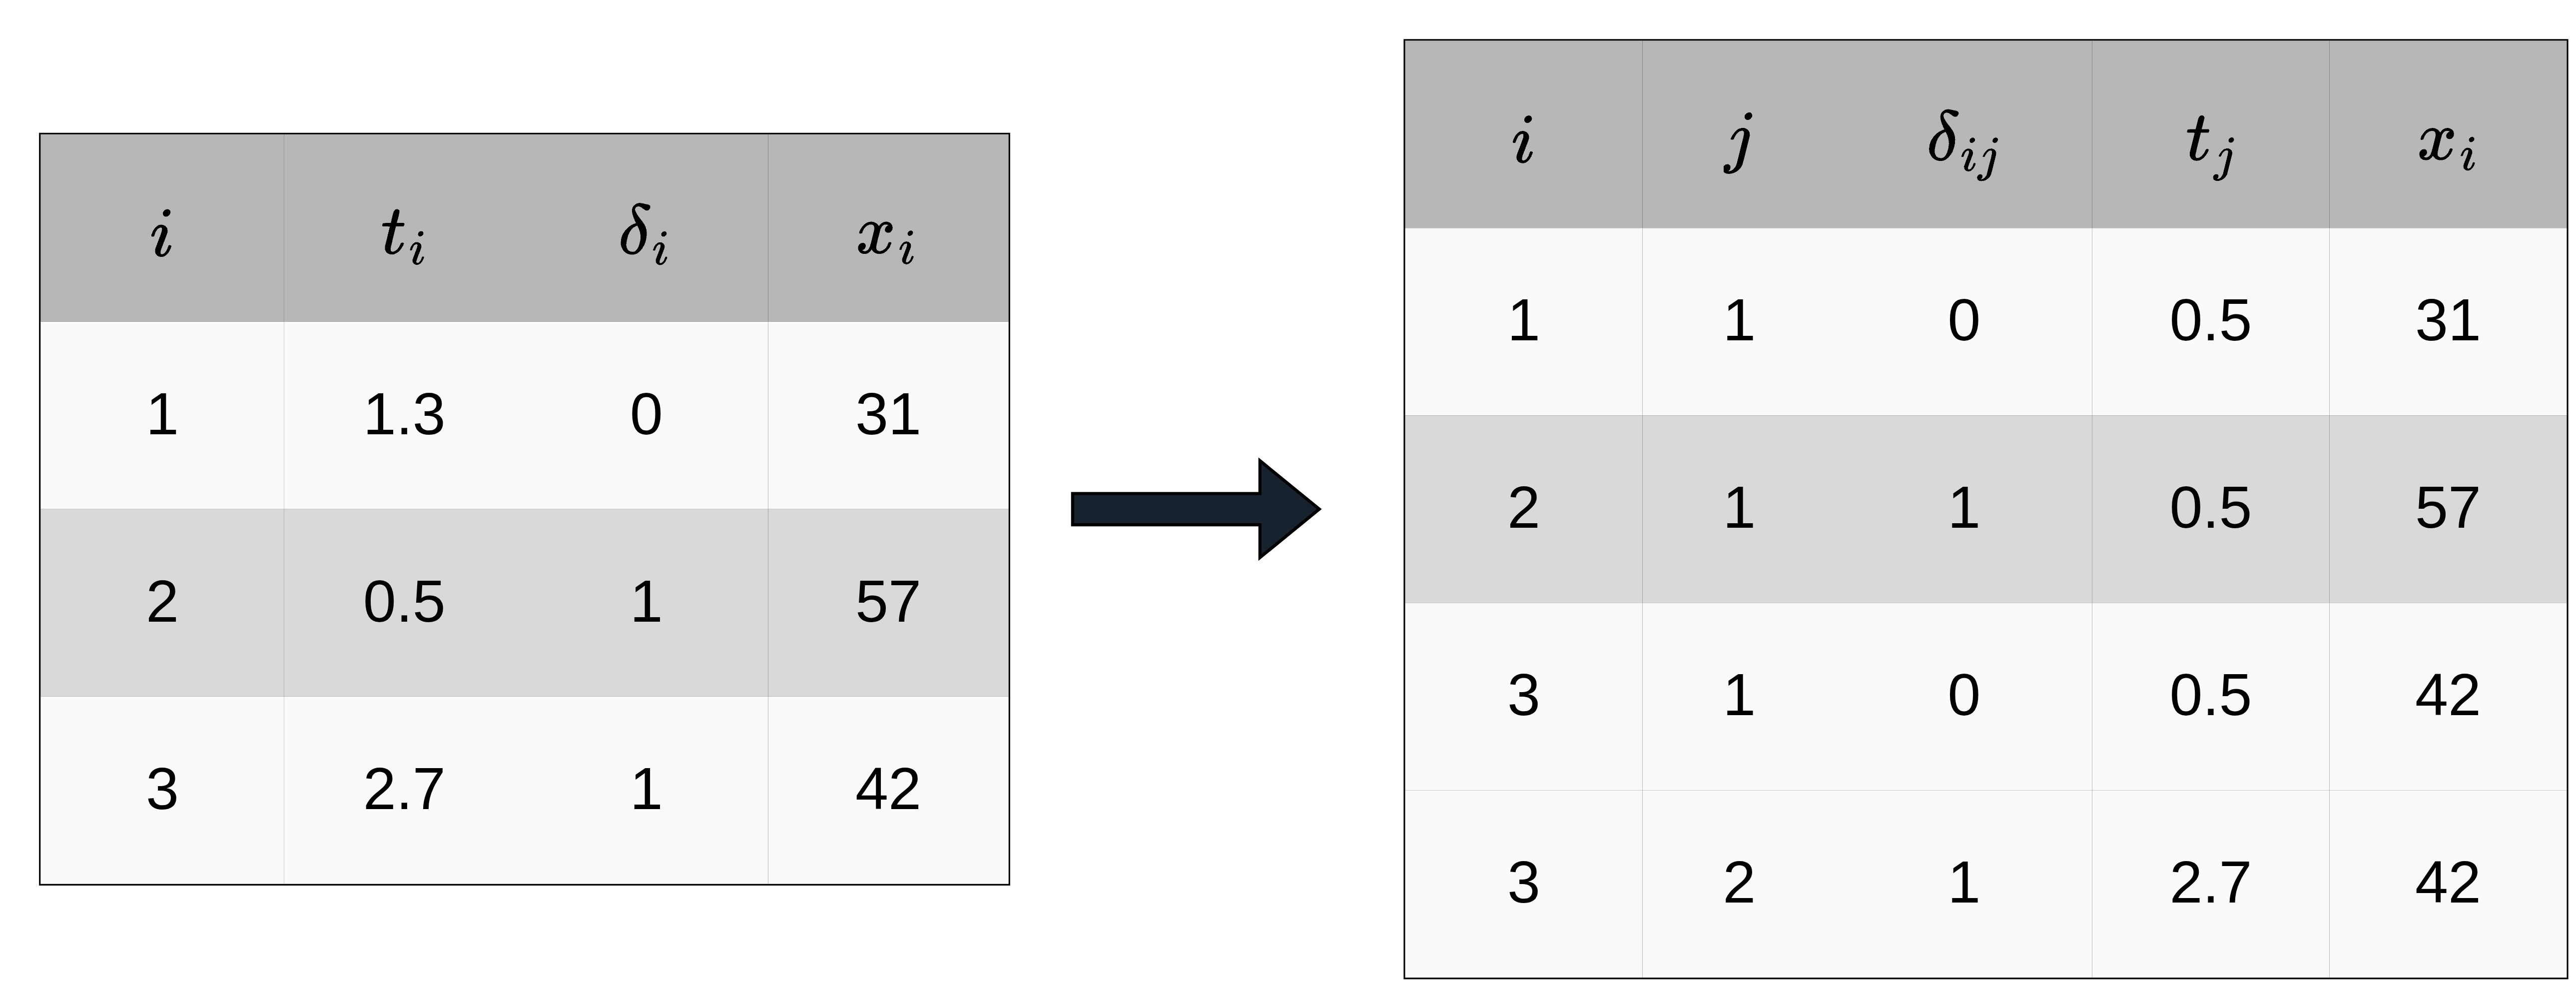
\includegraphics[width=1\linewidth,height=\textheight,keepaspectratio]{Figures/reductions/fig-p4c22-data-trafo-stacking.png}

}

\caption{\label{fig-p4c22-data-trafo-stacking}Illustration of the data
transformation for survival stacking, keeping only the columns needed
for stacking. Left: data in standard time-to-event format. Right: the
stacked dataset, with one row per subject per unique observed event time
at which the subject is at risk.}

\end{figure}%

Survival stacking yields data:

\[
\mathcal{D}_{\mathcal{A}} = \{(\delta_{ij}, \mathbf{x}_{ij}, t_{j})\}_{i=1,\ldots,n;\ j=1,\ldots,m:\ i \in \mathcal{R}_{t_{(j)}}},
\]

where the \(\delta_{ij}\) are the binary targets and \(t_j = t_{(j)}\)
is the event time, used as the time-representation feature
(Section~\ref{sec-partition-timerep}). As before, any algorithm that
returns binary class probabilities can be used for estimation.

The relationship to the discrete-time reduction becomes concrete when
the interval boundaries are set to the unique event times. Let
\(\mathcal{A} = \{t_{(1)}, \ldots, t_{(m)}, t_{(m+1)}\}\) be the
boundary points for a discrete-time reduction
(Section~\ref{sec-discrete-time-reduction}), where \(t_{(m+1)}\) is an
arbitrary time point after the last observed event time \(t_{(m)}\).
This defines intervals \(I_j = [t_{(j)}, t_{(j+1)})\) for
\(j = 1,\ldots,m\). Although this differs from the
infinitesimal-interval description of survival stacking,
\(I_j = [t_{(j)}, t_{(j)}+\,\mathrm{d}u)\), the number of events and the
number at risk are identical for both interval definitions, because no
events occur between two event times Therefore, survival stacking and
the discrete-time reduction with intervals defined by the unique
observed event times estimate the same discrete hazards
(\ref{eq-discrete-hazard-probability}) and produce the same survival
probabilities (\ref{eq-discrete-survival}). \[
\Pr\!\left(Y \in [t_{(j)}, t_{(j)}+\,\mathrm{d}u) \mid Y \geq t_{(j)}\right) = \Pr\!\left(Y \in [t_{(j)}, t_{(j+1)}) \mid Y \geq t_{(j)}\right) = h_{\tilde{Y}}(j).
\]

This perspective is useful because it allows survival stacking to be
implemented using standard discrete-time software for pre- and
post-processing.

\section{Piecewise constant
hazards}\label{sec-piecewise-constant-hazards}

The piecewise constant hazards approach, also known as the piecewise
exponential model (PEM), assumes the \emph{continuous-time} hazard
function is a step function: constant within each interval but allowed
to vary between
intervals.\index{reduction!partition reductions!piecewise exponential model}
The name comes from the fact that the hazard function of an exponential
distribution is constant. Thus, assuming a constant hazard within each
interval is equivalent to assuming that event times within that interval
follow an exponential distribution. In contrast to the discrete-time
approach (Section~\ref{sec-discrete-time-reduction}), which only models
\emph{whether} an event occurs within each interval, PEM uses the exact
within-interval event time and yields a continuous-time hazard estimate.
Intuitively, any underlying continuous hazard function can be
approximated arbitrarily well given enough intervals (and events).

Consider the partitioning of the follow-up as defined in
(\ref{eq-cut-points}) and assume that within each interval
\(I_j = [a_{j-1}, a_j)\), the hazard function is constant,

\begin{equation}\phantomsection\label{eq-constant-hazard}{
h(\tau) = h_j,\ \forall\ \tau \in I_j.
}\end{equation}

Note that left-closed, right-open intervals are used here for
consistency with the discrete-time approach in
Section~\ref{sec-discrete-time-reduction}. Usually in the PEM
literature, intervals are defined as left-open, right-closed (see also
Section~\ref{sec-choice-of-interval-boundaries}).

First, consider the likelihood contribution of subject \(i\) under the
piecewise-exponential assumption (\ref{eq-constant-hazard}). Recall from
Section~\ref{sec-distributions-continuous} the right-censored likelihood
and survival-hazard identity, \[
\mathcal{L}_i = h(t_i)^{\delta_i}\, S(t_i), \qquad S(t) = \exp\!\left(-\int_0^t h(u)\,\,\mathrm{d}u\right).
\]

Combining these,

\begin{equation}\phantomsection\label{eq-pem-likelihood-general}{
\begin{aligned}
\mathcal{L}_{i}
& = h(t_i)^{\delta_{i}}S(t_i)\\
& = h(t_i)^{\delta_{i}}\exp\left(-\int_{0}^{t_i} h(u) \ \,\mathrm{d}u\right)\\
& = h_{J_i}^{\delta_{i}}\exp\left(-\left[\sum_{j=1}^{J_i-1} (a_j - a_{j-1})h_j + (t_i - a_{J_i-1})h_{J_i}\right]\right)\\
& = h_{J_i}^{\delta_{i}}\exp\left(-\sum_{j=1}^{J_i} h_j t_{ij}\right) = h_{J_i}^{\delta_{i}}\prod_{j=1}^{J_i}\exp\left(- h_j t_{ij}\right)\\
& = \prod_{j=1}^{J_i} h_j^{\delta_{ij}} \exp(-h_j t_{ij}),
\end{aligned}
}\end{equation}

where the third and fourth equalities follow from the assumption that
the hazard is a step function (\ref{eq-constant-hazard}) and the
definition of time at risk (\ref{eq-time-at-risk}), and the last
equality uses the property \(\delta_{iJ_i} = \delta_i\) with
\(\delta_{ij}=0\) for \(j<J_i\) from (\ref{eq-interval-indicator}).

Now assume that the interval-specific event indicators \(\delta_{ij}\)
are realizations of random variables
\(\Delta_{ij} \stackrel{iid}{\sim} \text{Poisson}(\mu_{ij} := h_j t_{ij})\)
and recall that \(Z\sim \text{Poisson}(\mu)\) implies
\(\Pr(Z = z) = (\mu^z \exp(-\mu))/z!\). Thus, the likelihood
contribution of subject \(i\) can be written as:

\begin{equation}\phantomsection\label{eq-pem-poisson-likelihood}{
\begin{aligned}
\mathcal{L}_{\text{Poisson},i} 
& = \prod_{j=1}^{J_i} \Pr(\Delta_{ij} = \delta_{ij}) \\
&= \prod_{j=1}^{J_i} \frac{(h_j t_{ij})^{\delta_{ij}} \exp(-h_j t_{ij})}{\delta_{ij}!}\\
& = \prod_{j=1}^{J_i} h_j^{\delta_{ij}} t_{ij}^{\delta_{ij}}\exp(-h_j t_{ij}),
\end{aligned}
}\end{equation}

where the last equality follows from \(\delta_{ij} \in \{0,1\}\) and
\(0!=1!=1\).

Note that \(\mathcal{L}_{\text{Poisson}, i} \propto \mathcal{L}_i\) from
equation (\ref{eq-pem-likelihood-general}), since \(t_{ij}\) is a
constant and does not depend on the parameters of interest (here
\(h_j\)). This implies that the model with piecewise constant hazards
can be estimated by optimizing the Poisson likelihood
(\ref{eq-pem-poisson-likelihood}). The \(t_{ij}\) term enters as an
offset \(\log(t_{ij})\) in the Poisson regression model.

More generally, in the presence of features \(\mathbf{x}_{ij}\), assume
\(\delta_{ij} \mid \mathbf{x}_{ij} \stackrel{iid}{\sim} \text{Poisson}(\mu_{ij})\),
where \(\mu_{ij} = h_{ij} t_{ij}\) is the expected number of events in
interval \(j\) given features \(\mathbf{x}_{ij}\) and
\(h_{ij} = g(\mathbf{x}_{ij}, t_j\mid\boldsymbol{\theta})\) is the
hazard rate in interval \(j\) given features \(\mathbf{x}_{ij}\). This
can be estimated by fitting a Poisson regression model with log-link to
the transformed dataset\index{Poisson regression}

\[
\mathcal{D}_{\mathcal{A}} = \{(\delta_{ij}, \mathbf{x}_{ij}, t_{ij}, t_j)\}_{i=1,\ldots,n; j=1,\ldots,J_i},
\]

where the model specification is:

\begin{equation}\phantomsection\label{eq-pem-model}{
\log(\mathbb{E}(\Delta_{ij})) = \log(h_{ij}) + \log(t_{ij}),
}\end{equation}

where
\(\log(h_{ij}) =\log(g(\mathbf{x}_{ij}, t_j\mid\boldsymbol{\theta}))\)
is the interval- and feature-specific log-hazard function, \(g(\cdot)\)
is a function learned by the model of choice, and \(\log(t_{ij})\) is
included as an offset term in the Poisson likelihood/loss function.

The fitted model returns interval-specific hazard estimates
\(\hat{h}_j(\mathbf{x}) = g(\mathbf{x}, t_j \mid \hat{\boldsymbol{\theta}})\).
Survival probabilities follow from the cumulative hazard via
\(\hat{S}(\tau \mid \mathbf{x}) = \exp\left(-\int_0^\tau \hat{h}(u \mid \mathbf{x})\,\,\mathrm{d}u\right)\).
Because the hazard is piecewise constant, the integral reduces to a sum
of areas:

\[
\hat{S}(\tau \mid \mathbf{x}) = \exp\!\left(-\left[\sum_{j: a_j \leq \tau} \hat{h}_j(\mathbf{x})\,(a_j - a_{j-1}) \;+\; \hat{h}_{J_\tau}(\mathbf{x})\,(\tau - a_{J_\tau-1})\right]\right),
\]

where \(J_\tau\) is the index of the interval containing \(\tau\). The
first sum accumulates the hazard over completed intervals before
\(\tau\), and the trailing term adds the partial-interval contribution
from \(a_{J_\tau-1}\) up to \(\tau\).

One benefit of piecewise exponential models is that they preserve the
exact within-interval event time through the offset \(\log(t_{ij})\), so
no information is lost by discretizing the follow-up time. Because the
hazards are continuous-time, survival probabilities at any \(\tau\) are
obtained without interpolation. However, in contrast to other methods,
PEM requires a Poisson regression with offset, which fewer software
implementations support directly compared to vanilla binary
classification. Another drawback is that fitted hazards are continuous
rates rather than per-interval probabilities, which some practitioners
may find less intuitive than modeling \(h_{\tilde{Y}}(j)\).

To illustrate the piecewise constant hazards approach, consider again
the \texttt{tumor} dataset. First, the follow-up time is partitioned
into \(J = 100\) equidistant intervals. Then, a Poisson regression model
is fit with an interaction between interval and complications to allow
for separate baseline hazards in each complications group:

\[
\log(\mu_{ij}) = \log(\mathbb{E}(\Delta_{ij})) = \underbrace{\beta_{0j} + \beta_{1j}x_{i1}}_{\log(h_{ij})} + \log(t_{ij}),
\]

where \(x_{i1} = \mathbb{I}(\text{complications}_i = \text{``yes''})\),
\(\beta_{0j}\) are the interval-specific intercepts for the reference
group (no complications), \(\beta_{1j}\) are the deviations from the
reference group for the complications group, and \(\log(t_{ij})\) enters
as a known offset (fixed by the data). Concretely, fitting the model on
\(\mathcal{D}_{\mathcal{A}}\) uses \(\delta_{ij}\) as the response,
\(\mathbf{x}_{ij}\) and \(t_j\) as features. Estimation can be performed
by any method that can handle the Poisson likelihood (with offset) as
the objective function.

Figure~\ref{fig-p4c22-pem-interaction} shows the estimated survival
probabilities from the piecewise exponential model together with the
Kaplan-Meier estimates for comparison, with the model encoded by line
type and complications status by line color. The PEM provides an
excellent fit to the data, closely approximating the Kaplan-Meier
estimates.

\begin{figure}

\centering{

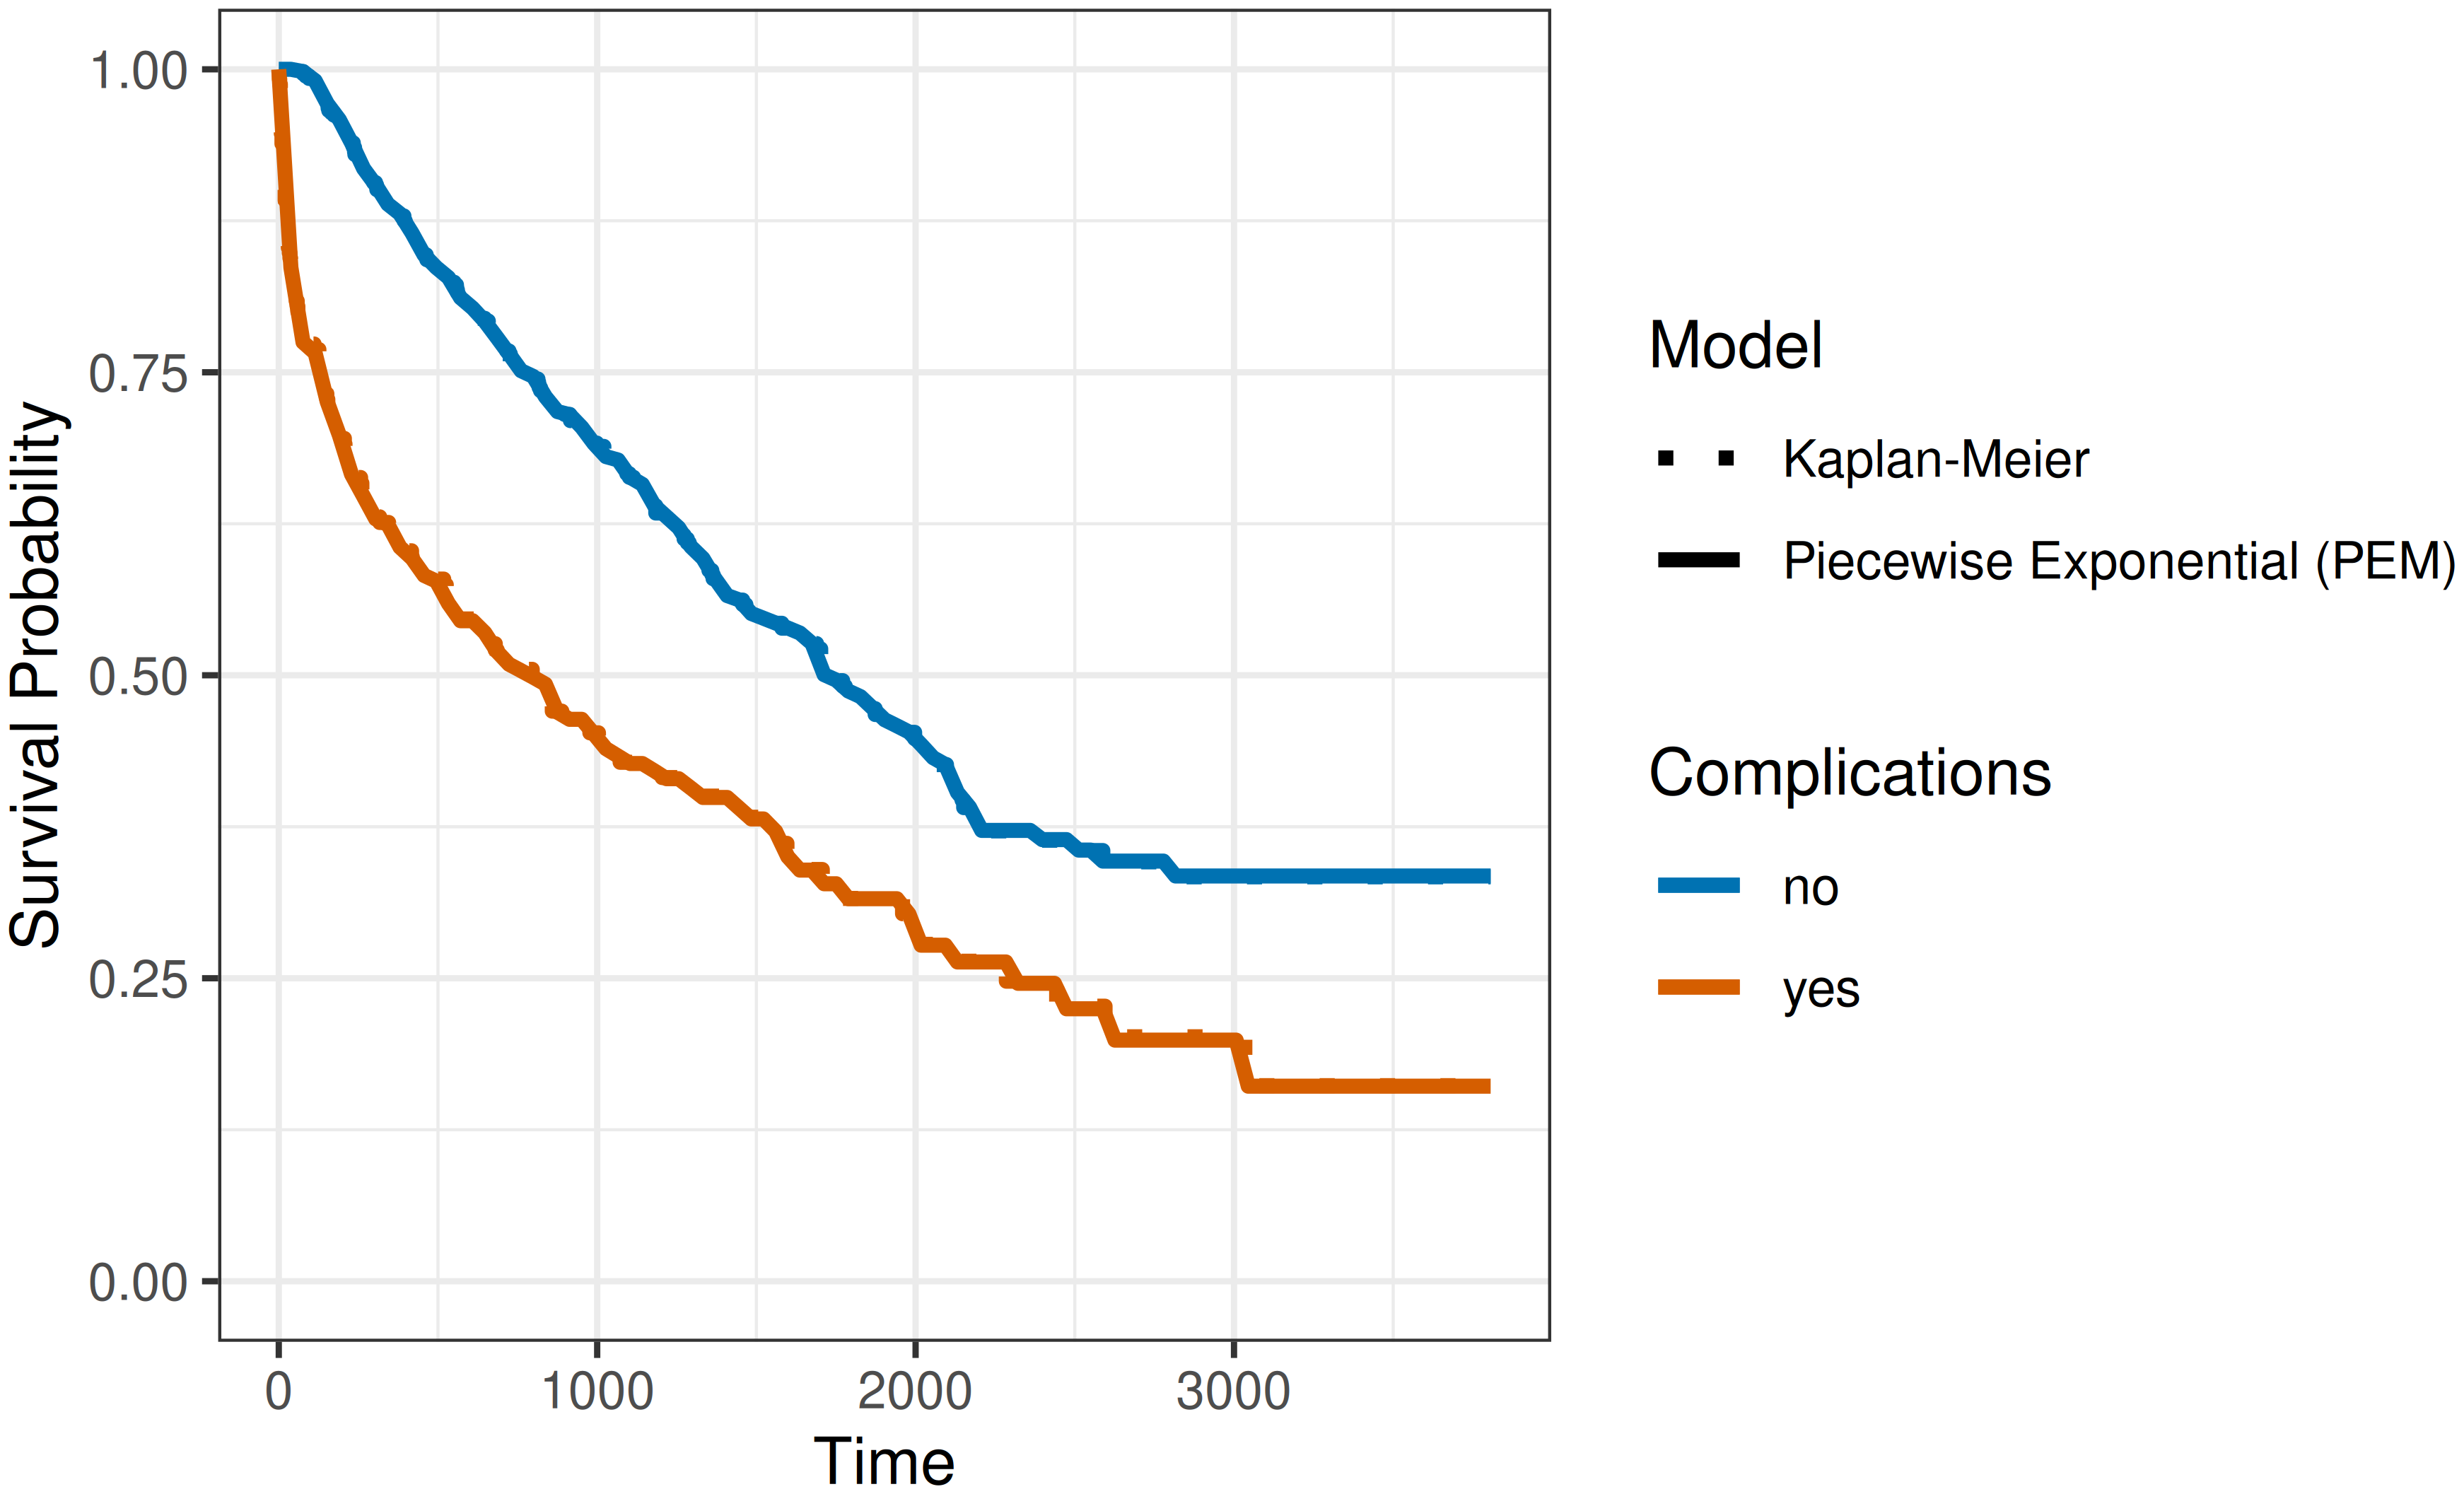
\includegraphics[width=0.7\linewidth,height=\textheight,keepaspectratio]{Figures/reductions/fig-p4c22-pem-interaction.png}

}

\caption{\label{fig-p4c22-pem-interaction}Comparison of survival
probability estimates using the piecewise exponential model (Poisson
regression) and the Kaplan-Meier estimator, for patients with and
without complications.}

\end{figure}%

\section{Choice of interval
boundaries}\label{sec-choice-of-interval-boundaries}

The reduction approaches introduced in the previous sections all depend
on the choice of the partition \(\mathcal{A}\) (\ref{eq-cut-points}).
This section discusses the practical considerations involved in
selecting interval boundaries, including the number and placement of cut
points, the conventions and considerations with respect to left-closed
versus left-open intervals, the representation of time within intervals,
and implications for left-truncated data.

\subsection{Number and placement of cut
points}\label{number-and-placement-of-cut-points}

The choice of the number of intervals \(J\) and the placement of the
interval boundaries \(a_j\) involves a trade-off between flexibility,
robustness, and computational cost. More intervals allow for a finer
approximation of the underlying hazard function, but at the cost of less
robust estimates (fewer events per interval) and a larger transformed
dataset. Fewer intervals yield more stable estimates but may miss
important variation in the hazard.

The simplest strategy is to use equidistant intervals, which does not
require any knowledge about the data but also does not adapt to it. A
more data-adaptive strategy is to use quantile-based intervals, which
place more cut points in regions with higher event density and fewer in
regions with sparse events.

A natural alternative is to use the unique, observed event times as cut
points, as done in survival stacking
(Section~\ref{sec-survival-stacking}). This mirrors the construction of
the Kaplan-Meier estimator and ensures that interval boundaries are
dense where events are frequent and sparse where they are rare. The same
strategy is the default in software packages for PEMs like
\texttt{pammtools} (Bender and Scheipl 2018). However, using all unique
event times can lead to very large transformed datasets. Since each of
the \(n\) subjects can contribute up to \(m\) rows, where \(m\) is the
number of unique event times, the transformed dataset contains
\(\tilde{n} = \sum_{i=1}^n J_i\) rows. Bender et al. (2021) showed that
using a random subsample of event times as cut points yields comparable
predictive performance while keeping the increase in dataset size linear
in the number of events, making this a practical strategy when \(m\) is
large.

\subsection{Left-closed or left-open
intervals}\label{sec-left-closed-vs-left-open}

Throughout this chapter, left-closed, right-open intervals
\([a_{j-1}, a_j)\) were used for consistency with the discrete-time
definitions in Section~\ref{sec-distributions-discrete}. This is the
natural convention for discrete-time/risk-set-based approaches (such as
Kaplan-Meier, Nelson-Aalen, and survival stacking), because all
observations before the event time are excluded from the risk set in the
interval \([t_{(j)}, t_{(j+1)})\), leading to the equivalence of the
discrete-time hazard and risk-set-based estimation (Tutz and Schmid
2016). However, in the PEM literature, left-open, right-closed intervals
\((a_{j-1}, a_j]\) are more commonly used, with the event times as cut
points and \(t_j = a_j\) (the right endpoint) (Bender and Scheipl 2018).

In most practical situations, the choice of convention has negligible
impact on the results; when intervals are small, both conventions
produce nearly identical estimates. The distinction matters primarily
when interval boundaries coincide with event times, as is the case in
survival stacking or when event times are used as cut points for PEM. In
this situation, with left-closed intervals \([a_{j-1}, a_j)\) and the
first cut point equal to the first event time, the interval
\([0, t_{(1)})\) contains no events. These event-free intervals should
be excluded from modeling, since the hazard is zero and the survival
probability one by definition. With left-open, right-closed intervals,
the first event time \(t_{(1)}\) is included in the first interval
\((0, t_{(1)}]\), avoiding this issue. Additionally, the definition of
the last interval is somewhat awkward when using left-closed intervals
since there is no natural endpoint; for example \([t_{(m)}, t_{(m)}+1)\)
and \([t_{(m)}, \infty)\) will yield the same number of zeros and ones
in the last interval and thus the same hazard function estimate.

\subsection{Representation of time within
intervals}\label{sec-partition-timerep}

The time representation feature \(t_j\) serves as the `time coordinate'
for interval \(j\) in the model. As introduced in
Section~\ref{sec-data-transformation}, one common choice is the interval
midpoint \(t_j = (a_{j-1} + a_j)/2\), but other choices include the
interval start point \(t_j = a_{j-1}\) or the endpoint \(t_j = a_j\).

The choice of \(t_j\) interacts with the interval convention. With
left-open, right-closed intervals \((a_{j-1}, a_j]\), the right endpoint
\(a_j\) is a natural representative because it is included in the
interval. With left-closed, right-open intervals \([a_{j-1}, a_j)\), the
left endpoint \(a_{j-1}\) is more natural, particularly when a smooth
function of \(t_j\) is estimated: the right endpoint \(a_J\) of the last
interval is not contained in that interval and the midpoint is arbitrary
because there is no natural endpoint for the last interval. For survival
stacking (Section~\ref{sec-survival-stacking}), the interval start point
\(t_j = t_{(j)}\) is used, since the event time itself defines the
interval.

A related modeling choice is whether \(t_j\) enters the model as a
categorical (factor) or continuous variable:

\begin{itemize}
\tightlist
\item
  When \(t_j\) is treated as a factor variable, the specific choice of
  \(t_j\) (midpoint, endpoint, etc.) is irrelevant. Each interval
  receives its own parameter (for example, an interval-specific
  intercept \(\beta_{0j}\)), as in the examples in
  Section~\ref{sec-discrete-time-reduction} and
  Section~\ref{sec-piecewise-constant-hazards}. This is the classical
  PEM approach and provides maximal flexibility, but assumes that the
  hazard in each interval is estimated independently of neighboring
  intervals. Without penalization, this can lead to implausible hazard
  estimates, especially when some intervals contain few events. The
  number of baseline hazard parameters equals \(J\), which becomes
  prohibitive when \(J\) is large (for example, when using all unique
  event times as cut points).
\item
  When \(t_j\) enters as a continuous variable, the specific choice of
  \(t_j\) is generally of minor importance, except possibly for the
  final interval and depending on the interval convention. In this
  setting, a functional relationship between time and the (log-)hazard
  is assumed. A linear relationship
  \(\log(h_j) = \beta_0 + \beta_1 t_j\) implies that the log-hazard
  changes at a constant rate over time, which is often too restrictive
  in practice. Instead, the relationship could be modeled flexibly
  (Section~\ref{sec-nonlinear}), for example as \(\log(h_j) = f(t_j)\)
  using penalized splines (Bender et al. 2018; Kopper et al. 2022) or
  tree-based methods (Bender et al. 2021). In this case, the number of
  baseline hazard parameters depends on the complexity of \(f\), not the
  number of intervals, making the approach scalable to fine partitions.
  Penalization encourages hazard estimates in neighboring intervals to
  be similar unless the data provides strong evidence for rapid
  changes.\index{penalization}
\end{itemize}

In practice, the continuous approach with some form of penalization or
regularized breakpoint detection (as in gradient boosted trees) combines
the flexibility of a fine partition with the stability of regularization
and is recommended when the number of intervals is moderate to large.

\subsection{Left-truncation}\label{sec-left-truncation-intervals}

When data are subject to left-truncation and delayed entry
(Section~\ref{sec-left-truncation}), the choice of interval boundaries
has additional implications.

The simplest case is when each subject's left-truncation time \(t_i^L\)
coincides with an interval boundary. Then, \(\delta_{ij}\) is defined
only for intervals \(j\) with \(a_{j-1} \geq t_i^L\), and
left-truncation is incorporated by excluding the earlier rows from the
transformed dataset \(\mathcal{D}_{\mathcal{A}}\).

If \(t_i^L\) does not coincide with an interval boundary, two options
are possible:

\begin{enumerate}
\def\labelenumi{\arabic{enumi}.}
\tightlist
\item
  Include only intervals for which subject \(i\) has been at risk from
  the start, \(a_{j-1} \geq t_i^L\). This is the most consistent with
  the risk-set-based approach.
\item
  Use the left-truncation times as additional cut points so no subject
  enters mid-interval. This guarantees correctness but enlarges the
  dataset and can introduce empty intervals; it is therefore only
  practical with a regularized baseline-hazard estimator.
\end{enumerate}

\section{Conclusion}\label{conclusion-15}

\begin{tcolorbox}[enhanced jigsaw, toprule=.15mm, bottomtitle=1mm, opacityback=0, breakable, leftrule=.75mm, title={Key takeaways}, toptitle=1mm, bottomrule=.15mm, colback=white, colframe=quarto-callout-warning-color-frame, titlerule=0mm, opacitybacktitle=0.6, coltitle=black, rightrule=.15mm, left=2mm, colbacktitle=quarto-callout-warning-color!10!white, arc=.35mm]

\begin{itemize}
\tightlist
\item
  Partition-based reductions transform survival data into a long-format
  dataset with one row per subject per interval at risk, enabling
  standard regression and classification methods to be applied to
  time-to-event data.
\item
  The discrete-time reduction and survival stacking estimate
  interval-specific discrete hazards via binary classification, while
  the piecewise exponential model estimates continuous-time hazards via
  Poisson regression with an offset.
\item
  A wide range of machine learning methods, including gradient boosting,
  neural networks, and random forests, can be used as base learners
  without modifying the underlying learning algorithm.
\item
  The choice of interval boundaries \(\mathcal{A}\) involves a trade-off
  between flexibility and computational cost; using unique event times
  is data-adaptive but can substantially increase dataset size.
\item
  The transformed dataset can be much larger than the original, and
  discrete-time approaches lose information about the exact event time
  within intervals unless very fine partitions are used.
\end{itemize}

\end{tcolorbox}

\begin{tcolorbox}[enhanced jigsaw, toprule=.15mm, bottomtitle=1mm, opacityback=0, breakable, leftrule=.75mm, title={Further reading}, toptitle=1mm, bottomrule=.15mm, colback=white, colframe=quarto-callout-tip-color-frame, titlerule=0mm, opacitybacktitle=0.6, coltitle=black, rightrule=.15mm, left=2mm, colbacktitle=quarto-callout-tip-color!10!white, arc=.35mm]

\begin{itemize}
\tightlist
\item
  M. Friedman (1982) introduced the piecewise exponential model and
  established its consistency properties.
\item
  Tutz and Schmid (2016) provide a comprehensive treatment of
  discrete-time survival analysis, covering model specification,
  estimation, and interpretation in depth.
\item
  Argyropoulos and Unruh (2015) and Bender, Groll, and Scheipl (2018)
  show how penalized additive models (PAMs) can be used as the base
  learner in the PEM framework, with the \texttt{pammtools} package
  (Bender and Scheipl 2018) providing a convenient implementation.
\item
  Bender et al. (2021) define a general PEM-based machine learning
  framework and study the effect of the number and placement of cut
  points on predictive performance.
\item
  Craig, Zhong, and Tibshirani (2025) provide a review of survival
  stacking and its connections to pooled logistic regression and the Cox
  model.
\end{itemize}

\end{tcolorbox}

\chapter{Reductions for Event History
Analysis}\label{sec-reductions-eha}

Chapter~\ref{sec-eha} introduced event history analysis, showing that
more complex time-to-event settings, including competing risks and
multi-state models, can be characterized by cause-specific or
transition-specific hazards. In particular, the cumulative incidence
function (CIF) (\ref{eq-cif}) was shown to depend on all cause-specific
hazards, and transition probabilities in multi-state models were
expressed via the product integral over all transition-specific hazards
(\ref{eq-ms-prodint-cumu-hazards}).

This chapter leverages those relationships to formulate event history
analysis as a reduction to multiple single-event hazard estimation
problems.\index{event history analysis}\index{reduction!event history reductions}
The key principle is to separately model each cause as the event of
interest and treat the others as censoring events, repeating this for
all possible causes. This enables any distribution-predicting
single-event model to be applied in the more general event history
setting by first predicting the cause-specific survival distributions
and then combining them into CIFs or transition probabilities.

\section{Competing risks: cause-specific
hazards}\label{sec-cr-reduction}

Recall the competing-risks setting of Section~\ref{sec-competing-risks}:
subjects start in an initial state \(0\) and may transition to one of
\(Q\) absorbing states \(q \in \{1,\ldots,Q\}\), observed as data
\((\mathbf{x}_i, t_i, q_i)\) with \(q_i \in \{0\}\cup \{1,\ldots, Q\}\)
the status observed for subject \(i\), where \(q_i=0\) encodes
censoring.\index{competing risks}\index{cause-specific hazard function}\index{reduction!event history reductions!competing risks}
Recall also the cause-specific hazard \(h_q(\tau \mid \mathbf{x})\)
(\ref{eq-cause-specific-hazard}), cumulative hazard
\(H_q(\tau \mid \mathbf{x})\) (\ref{eq-cause-specific-cumu-hazard}), and
cumulative incidence function \(F_q(\tau \mid \mathbf{x})\)
(\ref{eq-cif}), as well as the all-cause survival probability
\(S(\tau \mid \mathbf{x})\) (\ref{eq-all-cause-surv-prob}), which is the
probability of remaining free of any event.

The reduction principle is to estimate each cause-specific hazard,
\(h_q\), separately by treating events of type \(q\) as the event of
interest and all others as censoring. The resulting hazard estimates are
then combined to estimate \(\hat{S}\) and \(\hat{F}_q\).
Section~\ref{sec-cr-separate} introduces this procedure by fitting each
cause independently, whereas Section~\ref{sec-cr-stacked} presents a
joint approach using a single stacked model.

\subsection{Separate datasets}\label{sec-cr-separate}

Figure~\ref{fig-p4c23-cr-reduction-pipeline} summarizes the
cause-specific estimation approach where causes are estimated separately
for three observations and two competing risks:

\begin{enumerate}
\def\labelenumi{\arabic{enumi}.}
\item
  \textbf{Create cause-specific datasets} (Training). For each cause
  \(q \in \{1,\ldots,Q\}\), define the cause-specific status,
  \(\delta_{i,q} = \mathbb{I}(q_i = q)\), such that cause \(q\) remains
  the event of interest and all other causes are treated as censored at
  time \(t_i\). Then, define the cause-specific dataset
  \(\mathcal{D}_q = \{(\mathbf{x}_i, t_i, \delta_{i,q})\}^n_{i=1}\).
\item
  \textbf{Fit \(Q\) single-event models} (Training). Fit any of the
  distribution-predicting methods in Part III or partition-based
  reduction methods in Chapter~\ref{sec-partition-based-reductions} to
  the cause-specific datasets, \(\mathcal{D}_q\).
\item
  \textbf{Predict cause-specific hazards} (Predicting). For each cause
  \(q \in \{1,\ldots,Q\}\), for a new observation \(\mathbf{x}_*\),
  predict the cause-specific hazard function,
  \(\hat{h}_q(\cdot \mid \mathbf{x}_*)\), or cause-specific cumulative
  hazard function, \(\hat{H}_q(\cdot \mid \mathbf{x}_*)\). If required,
  obtain the corresponding cumulative hazard or hazard function from the
  predicted quantity via the relationships in
  Section~\ref{sec-distributions-continuous}.
\item
  \textbf{Predict all-cause survival and CIFs} (Predicting). Combine the
  cause-specific cumulative hazards into the all-cause survival
  probability\index{cumulative incidence function}\index{all-cause survival function}
  (\ref{eq-all-cause-surv-prob}),

  \[
  \hat{S}(\tau\mid\mathbf{x}_*) = \exp\!\left(-\sum_{q=1}^{Q} \hat{H}_q(\tau\mid\mathbf{x}_*)\right),
  \]

  and compute the CIF (\ref{eq-cif}):

  \[
  \hat{F}_q(\tau \mid \mathbf{x}_*) = \int_{0}^\tau \hat{S}(u \mid \mathbf{x}_*) \hat{h}_q(u \mid \mathbf{x}_*)\ \,\mathrm{d}u,
  \]

  or the corresponding discrete form when the learner returns
  step-function (cumulative) hazards.
\end{enumerate}

\begin{figure}

\centering{

\includegraphics[width=0.9\linewidth,height=\textheight,keepaspectratio]{Figures/reductions/fig-p4c23-cr-reduction-pipeline.png}

}

\caption{\label{fig-p4c23-cr-reduction-pipeline}Cause-specific reduction
for competing-risks data. The original dataset (left) is split into one
cause-specific dataset per cause; each cause-specific dataset is then
passed to its own model; the per-cause hazard estimates are combined
into the all-cause survival probability
\(\hat{S}(\tau \mid \mathbf{x})\), and the cause-specific cumulative
incidence functions \(\hat{F}_q(\tau \mid \mathbf{x})\).}

\end{figure}%

The clear advantage of this approach is that the cause-specific models
are fitted independently. This provides considerable flexibility as, in
principle, each cause can be modeled using a different learning
algorithm, or the same algorithm with different hyperparameters.
Independent models also make training \emph{embarrassingly parallel}, as
each model can be fitted and tuned separately
(Section~\ref{sec-ml-opt}). However, fitting each cause independently
means no information is shared across models. This can be a disadvantage
when a cause has few events, since structure common to several causes,
such as a shared baseline-hazard shape or similar covariate effects,
cannot be exploited across them. A further, more practical drawback is
that each model estimates its cause-specific cumulative hazard
\(\hat{H}_q\) on its own time grid, so these estimates must be
interpolated onto a common grid before they can be combined into the
downstream quantities \(\hat{S}\) and \(\hat{F}_q\). This interpolation
is usually computationally inexpensive (see the random forest discussion
in Section~\ref{sec-surv-ml-models-ranfor-nodes}).

Returning to the \texttt{sir.adm} example from
Section~\ref{sec-cr-notation}: a Cox model
(Section~\ref{sec-classical-cox}) and a single-event random survival
forest (RSF; Chapter~\ref{sec-ranfor}) are fitted using the above
reduction (Figure~\ref{fig-p4c23-cif-marg-sir}). Both estimators use
pneumonia status at admission as their only covariate and target the
same stratified estimand. The resulting CIFs are compared to a
non-parametric Aalen-Johansen baseline. The reduction-based RSF closely
tracks the Aalen-Johansen baseline, with a small offset on the discharge
CIF (top panels). The Cox PH curves are also close to the Aalen-Johansen
estimates but again show differences for discharge, attributable to the
proportional-hazards constraint.

\begin{figure}

\centering{

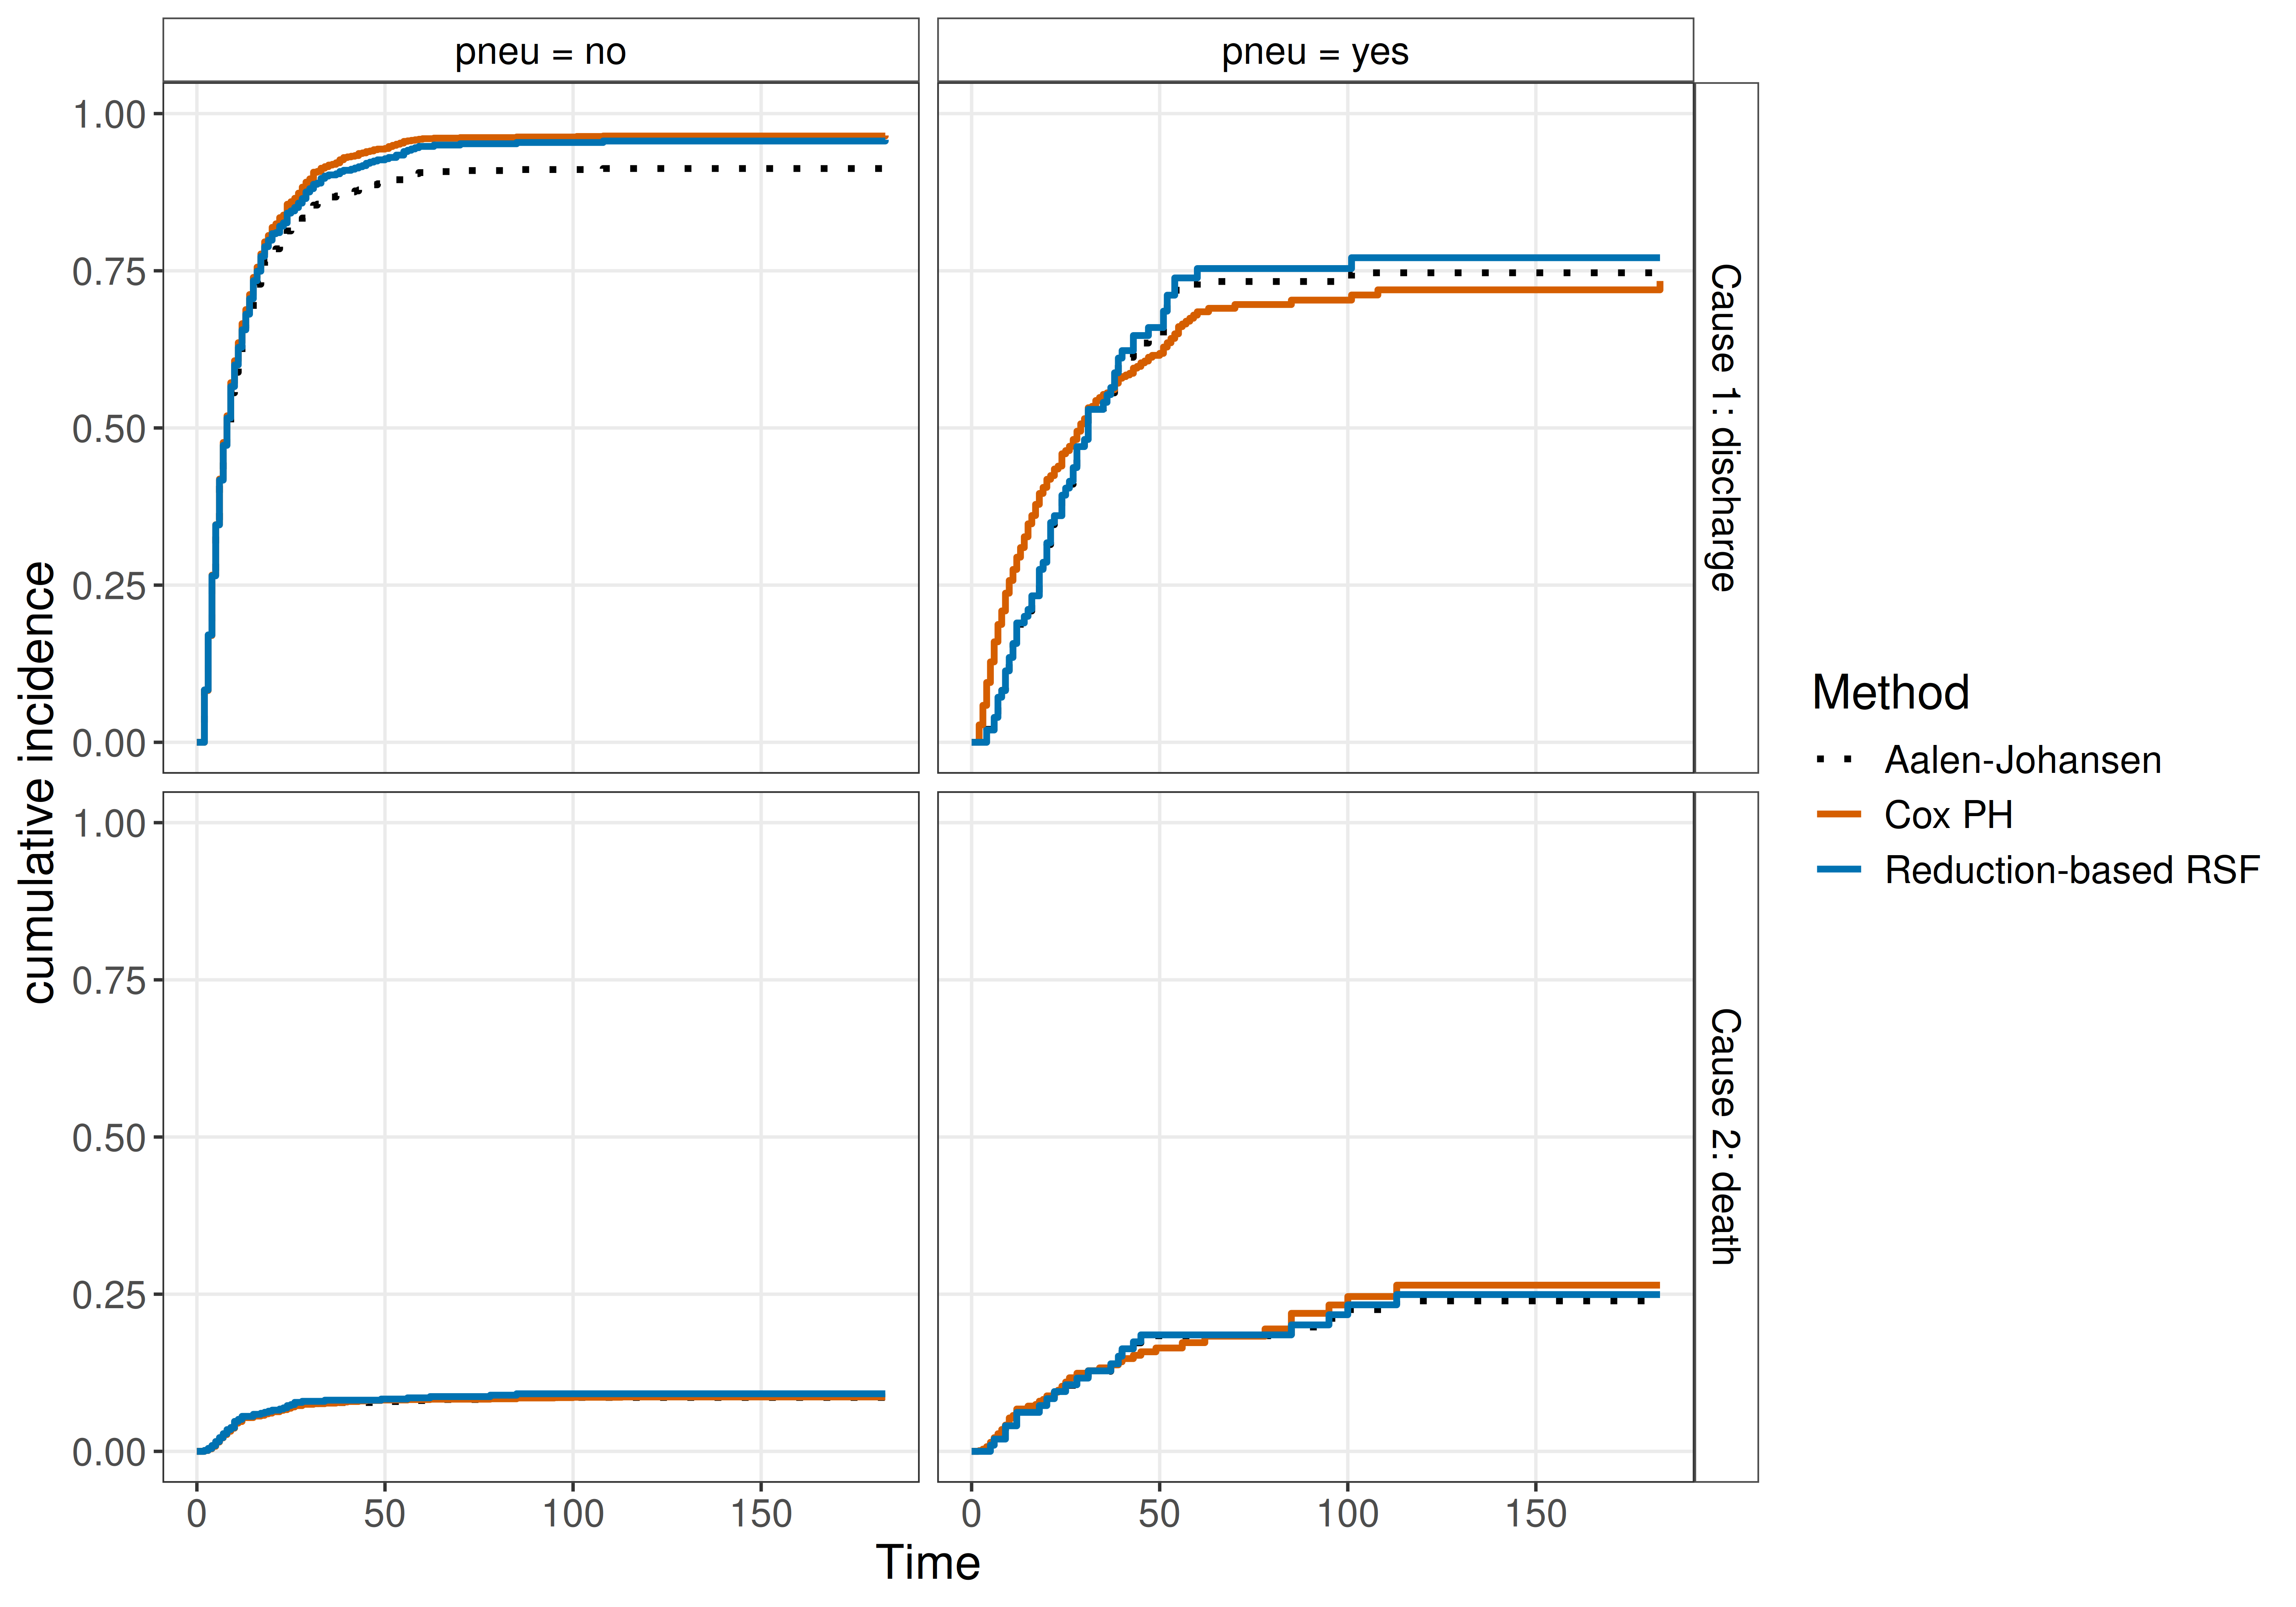
\includegraphics[width=0.8\linewidth,height=\textheight,keepaspectratio]{Figures/reductions/fig-p4c23-cif-marg-sir.png}

}

\caption{\label{fig-p4c23-cif-marg-sir}Cumulative incidence functions on
\texttt{sir.adm} for discharge (top row) and death (bottom row)
stratified by pneumonia status at admission (columns), as estimated by
the non-parametric Aalen-Johansen estimator, a cause-specific Cox PH
model, and a reduction-based random survival forest (two single-event
RSFs combined via the reduction). All three curves overlap closely,
illustrating that the cause-specific reduction is close to the
Aalen-Johansen estimator baseline.}

\end{figure}%

\subsection{Stacked dataset}\label{sec-cr-stacked}

Instead of estimating each cause-specific hazard through distinct
models, an alternative is to construct a single stacked model from one
dataset containing one row per (subject, cause) pair, with an additional
indicator \(c \in \{1, \ldots, Q\}\) recording which cause that row
represents. Figure~\ref{fig-p4c23-cr-reduction-stacked} illustrates the
construction.\index{reduction!event history reductions!competing risks}

\begin{figure}

\centering{

\includegraphics[width=0.9\linewidth,height=\textheight,keepaspectratio]{Figures/reductions/fig-p4c23-cr-reduction-stacked.png}

}

\caption{\label{fig-p4c23-cr-reduction-stacked}Stacked cause-specific
reduction. Each subject in the original competing risks dataset
contributes one row per cause \(c\) to a single stacked dataset (rows
shaded by \(c\) in the diagram), with \(\delta\) recording whether that
specific cause was the observed event. A single hazard learner with a
\(c \times \mathbf{x}\) interaction is fit, and cause-specific hazards
are recovered by evaluating the fitted model at fixed \(c\).}

\end{figure}%

This approach breaks the problem into the following steps:

\begin{enumerate}
\def\labelenumi{\arabic{enumi}.}
\item
  \textbf{Stack the cause-specific datasets} (Training). For each cause
  \(q \in \{1,\ldots,Q\}\), build \(\mathcal{D}_q\) by defining the
  cause-specific status: \(\delta_{i,q} = \mathbb{I}(q_i = q)\). Cause
  \(q\) remains the event of interest, all other causes are treated as
  censored at time \(t_i\), and the tuple
  \((\mathbf{x}_i, t_i, \delta_{i,q})\) is the observation for subject
  \(i\) in \(\mathcal{D}_q\). The cause-specific datasets are then
  concatenated row-wise into a single stacked dataset, augmented by an
  additional cause indicator \(c \in \{1, \ldots, Q\}\), which indicates
  the cause represented by each row, such that the stacked dataset will
  have \(Q\) rows for each of the \(n\) observations. In this example, a
  subject who experienced cause \(1\) thus contributes one row with
  \((c,\delta) = (1, 1)\) and a second row with \((c,\delta) = (2, 0)\).
\item
  \textbf{Fit a single stacked model} (Training). A single learner is
  fit to the entire stacked dataset with \(c\) included as a feature.
  Either a full \(c \times \mathbf{x}\) interaction can be added so each
  cause retains its own hazard structure, or interactions can be
  discovered automatically by a flexible learner (such as a random
  forest or neural network).
\item
  \textbf{Predict cause-specific hazards} (Predicting). Predictions of
  the cause-specific hazard are made by conditioning the fitted hazard
  on the cause. For a new observation \(\mathbf{x}_*\), \[
  \hat{h}_q(\tau \mid \mathbf{x}_*) = \hat{h}(\tau \mid \mathbf{x}_*, c = q), \quad q \in \{1,\ldots,Q\}.
  \]
\item
  \textbf{Predict all-cause survival and CIFs} (Predicting). Combine the
  cause-specific hazards into all-cause survival and CIF predictions
  using the same process as in the separate cause approach
  (Section~\ref{sec-cr-separate}).
  \index{cumulative incidence function}\index{all-cause survival function}
\end{enumerate}

This approach addresses some of the limitations of
Section~\ref{sec-cr-separate}. In particular, information can be shared
across causes through common parameters, and implementation is
simplified as only a single model must be fitted and tuned. However, the
stacked dataset is \(Q\) times larger than the original, and the learner
must be capable of modeling the \(c \times \mathbf{x}\) interaction
structure while allowing different baseline hazards for each cause.
Depending on the number of causes and the size of the original dataset,
this can make some simpler and more interpretable models
(Chapter~\ref{sec-classical}) impractical. Another drawback is the risk
of joint misspecification. In the separate approach, a misspecified
model affects only a single cause, whereas misspecification of a shared
model in the stacked approach will affect all causes simultaneously.
Finally, hyperparameter tuning may become more challenging. A single set
of hyperparameters must either be shared across all causes, potentially
leading to suboptimal performance for some causes, or additional model
complexity must be introduced to allow cause-specific flexibility.

\section{Multi-state: transition-specific
hazards}\label{sec-ms-reduction}

The reduction principle introduced for competing risks extends naturally
to multi-state
models.\index{multi-state models}\index{reduction!event history reductions!multi-state models}
Recall from Section~\ref{sec-multi-state} that subjects occupy states in
a finite state space and may transition between admissible state pairs
\((\ell, q)\), that is, pairs for which a transition is possible a
priori. Analogous to the competing risks reduction, this reduction makes
use of the transition-specific hazard\index{transition-specific hazard}
\(h_{\ell q}(\tau \mid \mathbf{x})\), cumulative transition hazard
\(H_{\ell q}(\tau \mid \mathbf{x})\), and
transition-probability\index{transition probability} matrix
\(\mathbf{P}(\zeta, \tau \mid \mathbf{x})\), which is recovered from the
cumulative hazards via the product integral
(Section~\ref{sec-ms-transition-probs}).

A key difference from the competing-risks reduction is process-induced
left-truncation
(Section~\ref{sec-left-truncation}).\index{truncation!left} In competing
risks, subjects typically start in state \(0\) at \(\tau = 0\). In
contrast, in a multi-state process a subject enters the risk set for a
transition \(\ell \to q\) only upon entering state \(\ell\), which
differs across subjects. A subject can only be at risk of leaving a
state after first entering it. For example, in the \texttt{prothr}
dataset of Section~\ref{sec-multi-state}, a subject who starts in
normal-prothrombin state (\(\ell = 0\)) enters the risk set for
transitions out of the abnormal state (\(\ell = 1\)) only at the time of
their first \(0 \to 1\) transition. This left-truncation must be handled
by each transition-specific model, which is a non-trivial drawback of
the method as left-truncation is rarely implemented in contemporary
software packages.

\subsection{Separate datasets}\label{sec-ms-transition-datasets}

Similar to the competing risks case, this multi-state reduction pipeline
builds one dataset per admissible transition and fits one model to each.
Figure~\ref{fig-p4c23-ms-reduction-pipeline} summarizes the construction
for an illness-death model with recovery, with states \(\{0, 1, 2\}\)
and four admissible transitions: \(0\to1\), \(0\to2\), \(1\to0\),
\(1\to2\):

\begin{enumerate}
\def\labelenumi{\arabic{enumi}.}
\item
  \textbf{Create transition-specific datasets} (Training). For each
  admissible transition, \(\ell \to q\), build a transition-specific
  dataset, \(\mathcal{D}_{\ell q}\) with one row for each spell during
  which a subject occupies state \(\ell\). For each spell, the dataset
  includes \(t_{i,\text{start}}\), the time at which subject \(i\)
  entered state \(\ell\) for that spell, \(t_{i,\text{stop}}\), the time
  at which they left the state or were censored, and
  \(\delta_{i,\ell q}\) which is \(1\) if they transitioned from
  \(\ell\) to \(q\) or \(0\) otherwise. Subjects therefore contribute to
  every transition-specific dataset for which they were at risk,
  \emph{but only} from their subject-specific entry time into that
  dataset. For example, in Figure~\ref{fig-p4c23-ms-reduction-pipeline},
  subject 1 only enters the \(1 \to 0\) and \(1 \to 2\) datasets at time
  \(2\), whereas subject \(2\) never even enters those datasets. When
  \(t_{i,\text{start}} > 0\), the subject is left truncated as they
  entered the state after the process began.
\item
  \textbf{Fit single-event models} (Training). Use the
  transition-specific datasets, \(\mathcal{D}_{\ell q}\), to fit any of
  the distribution-predicting methods in Part III or partition-based
  reduction methods in Chapter~\ref{sec-partition-based-reductions} that
  can handle left truncation.
\item
  \textbf{Predict transition-specific hazards} (Predicting). For each
  transition \(\ell \to q\), for a new observation \(\mathbf{x}_*\),
  predict the transition-specific hazards,
  \(\hat{h}_{\ell q}(\tau \mid \mathbf{x}_*)\), or cumulative hazards,
  \(\hat{H}_{\ell q}(\tau \mid \mathbf{x}_*)\). If required, the
  corresponding cumulative hazard or hazard function may then be
  obtained from the predicted
  quantity.\index{transition-specific hazard}
\item
  \textbf{Predict transition probabilities} (Predicting). Stack the
  predicted transition cumulative hazards into the matrix
  \(\hat{\mathbf{H}}(\tau \mid \mathbf{x}_*)\) with off-diagonal entries
  \(\hat{H}_{\ell q}\) and diagonal entries chosen such that each row
  sums to zero. The transition-probability
  matrix\index{transition probability} is then approximated via the
  product integral (\ref{eq-ms-prodint-approx}),

  \begin{equation}\phantomsection\label{eq-ms-prodint-approx-recall}{
  \hat{\mathbf{P}}(\zeta, \tau \mid \mathbf{x}_*) \approx \prod_{j=1}^{J}\bigl(\mathbf{I} + \boldsymbol{\Delta}\hat{\mathbf{H}}(t_j \mid \mathbf{x}_*)\bigr),
  }\end{equation}

  over a partition \(\zeta = t_0 < t_1 < \cdots < t_J = \tau\), where
  \(\boldsymbol{\Delta}\hat{\mathbf{H}}(t_j \mid \mathbf{x})\) is the
  matrix of cumulative-hazard increments in \((t_{j-1}, t_j]\).
\end{enumerate}

\begin{figure}

\centering{

\includegraphics[width=0.9\linewidth,height=\textheight,keepaspectratio]{Figures/reductions/fig-p4c23-ms-reduction-pipeline.png}

}

\caption{\label{fig-p4c23-ms-reduction-pipeline}Transition-specific
reduction for multi-state data. The original multi-state dataset (left)
is split into one dataset per admissible transition \(\ell \to q\); each
dataset is passed to a hazard learner that supports left-truncation; the
per-transition cumulative hazards
\(\hat{H}_{\ell q}(\tau \mid \mathbf{x})\) are then combined into the
transition probability matrix
\(\hat{\mathbf{P}}(\zeta, \tau \mid \mathbf{x})\) via the product
integral.}

\end{figure}%

Returning to the \texttt{prothr} example of
Section~\ref{sec-multi-state}, the reduction pipeline is illustrated
using a gradient boosting machine (GBM)
(Figure~\ref{fig-p4c23-tp-prothr-cmp}). Because few software
implementations support left-truncated data directly, the multi-state
task is first reduced to transition-specific single-event hazard
estimation with left-truncation
(Section~\ref{sec-ms-transition-datasets}), and then to a Poisson
regression task via the piecewise constant hazards reduction
(Section~\ref{sec-piecewise-constant-hazards}) (Bender et al. 2021). The
resulting fits show that the GBM reduction is closely aligned to the
Aalen-Johansen baseline across all four transitions and both treatment
arms.

\begin{figure}

\centering{

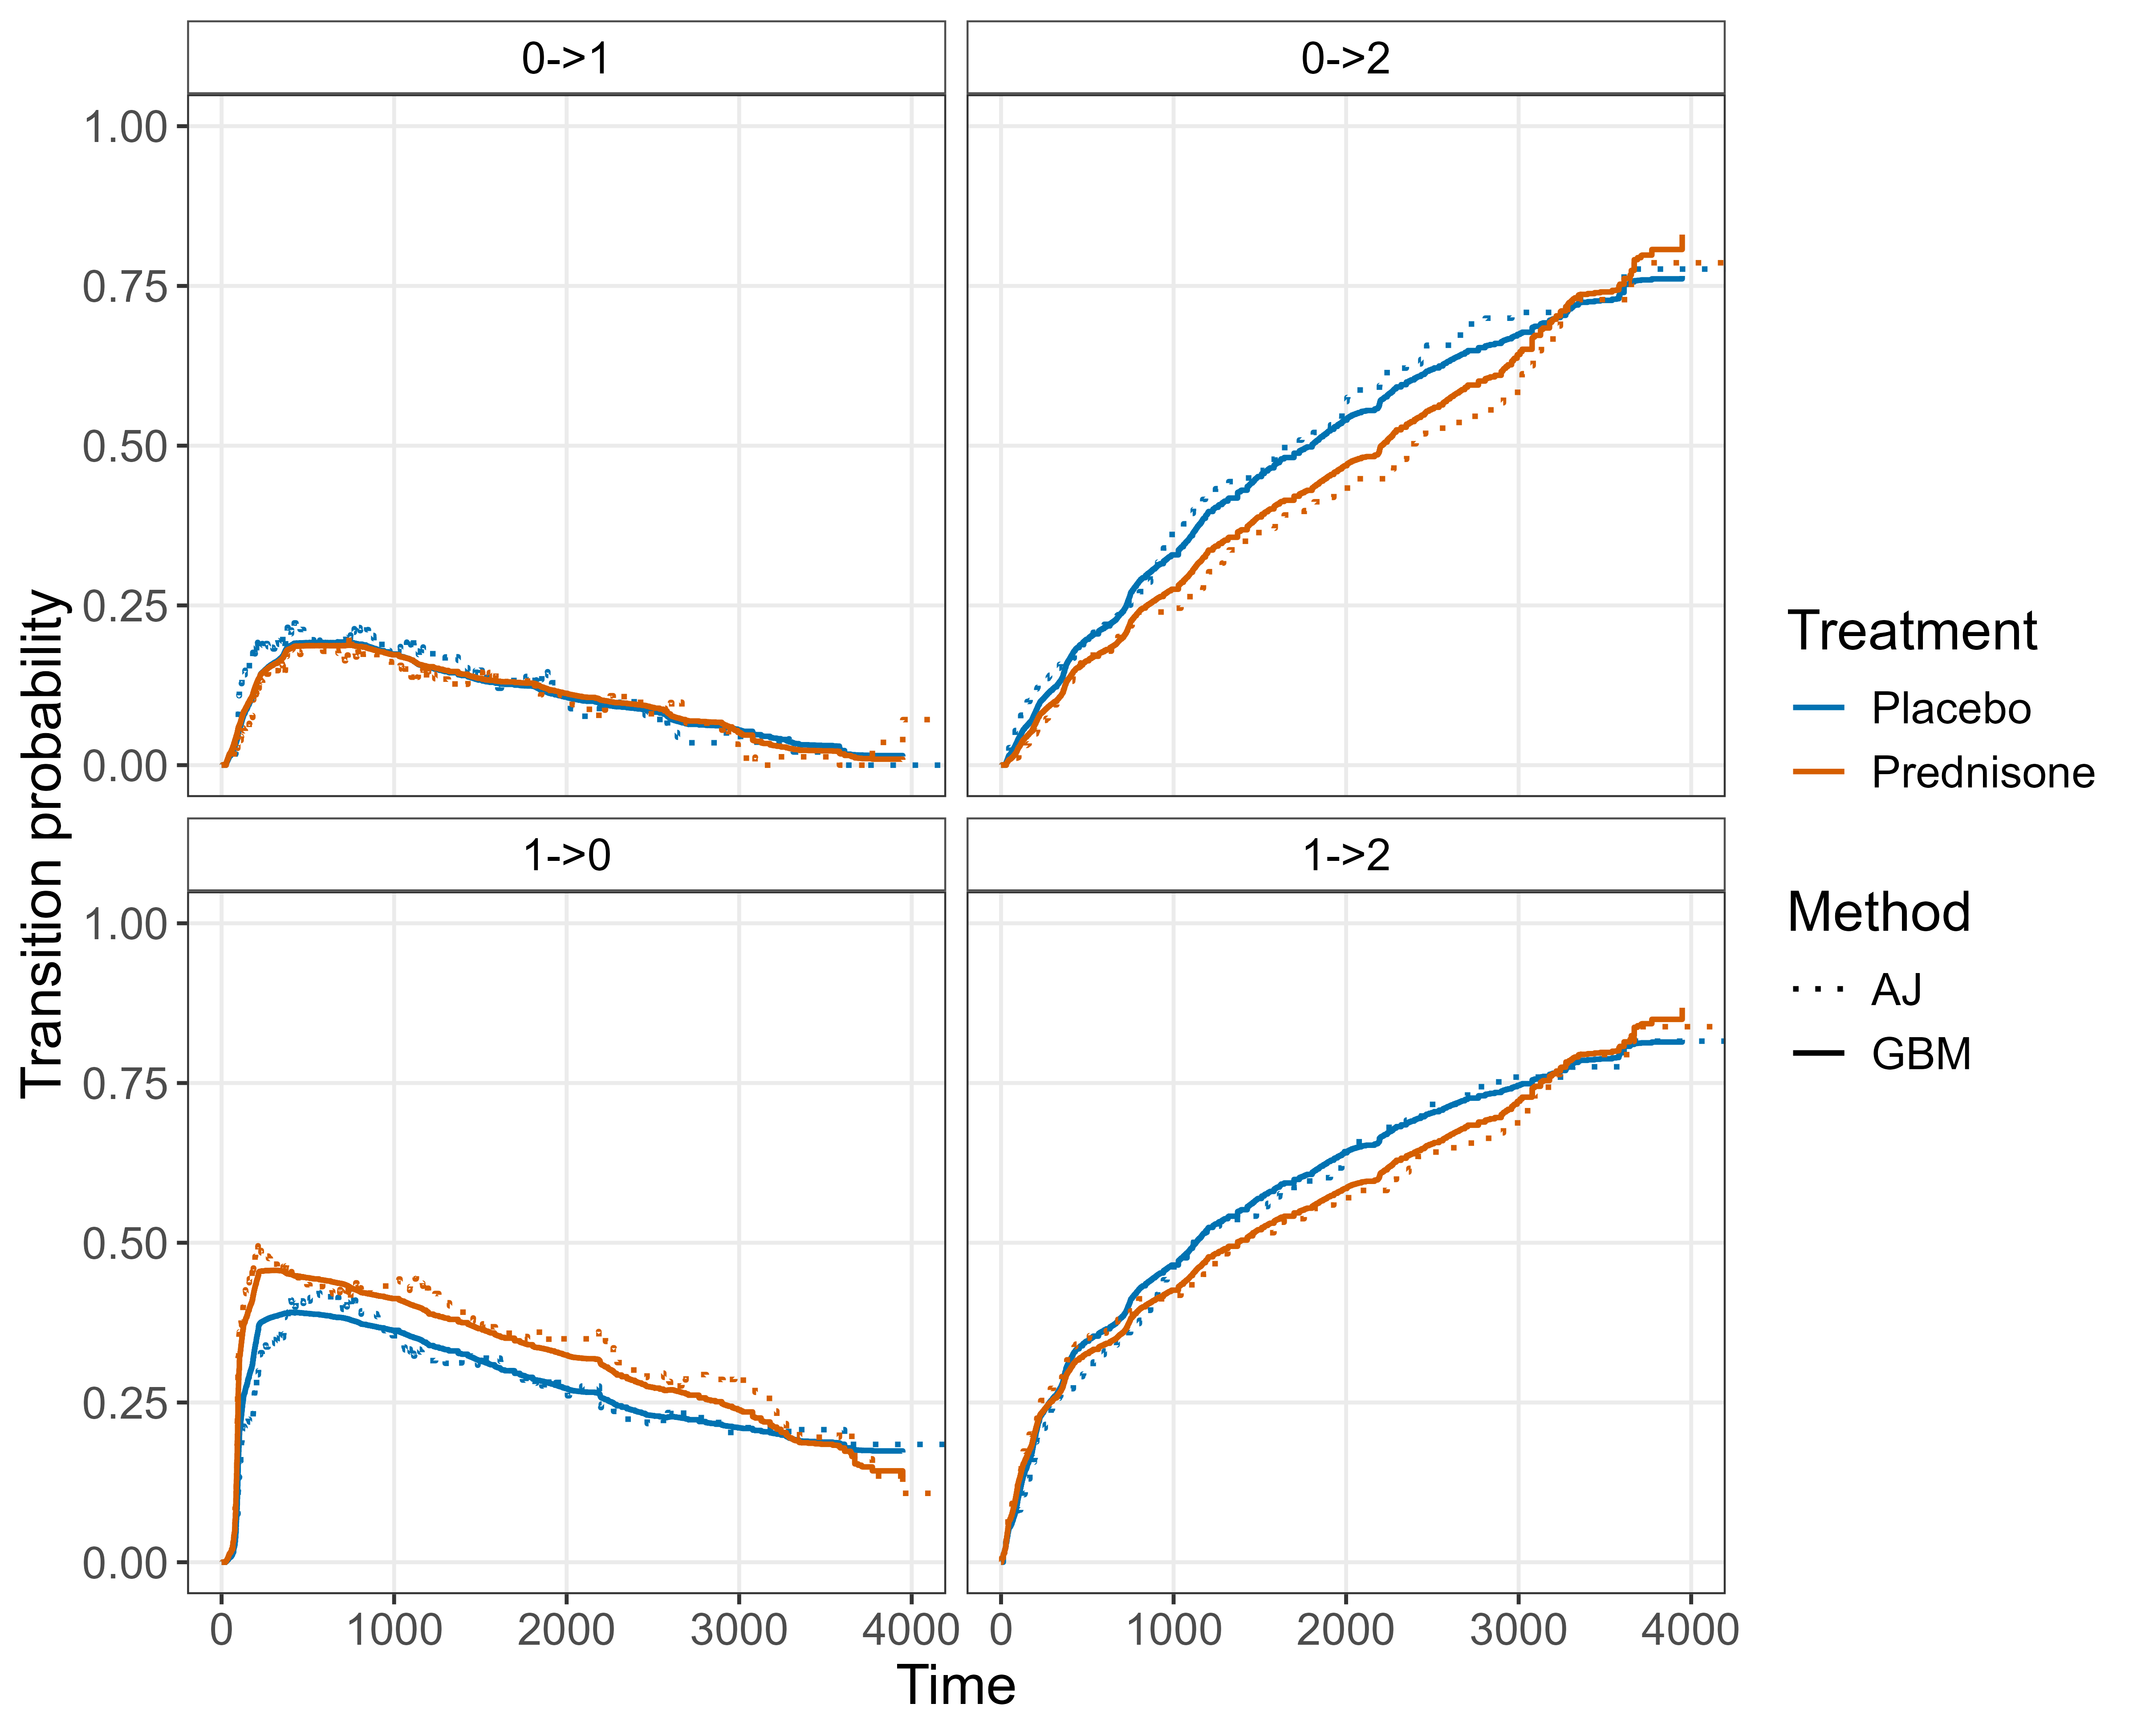
\includegraphics[width=0.8\linewidth,height=\textheight,keepaspectratio]{Figures/reductions/fig-p4c23-tp-prothr-cmp.png}

}

\caption{\label{fig-p4c23-tp-prothr-cmp}Transition probabilities on
\texttt{prothr} for the four admissible transitions \(\ell \to q\)
(panels), stratified by treatment, as estimated by two methods: the
non-parametric Aalen-Johansen estimator split by treatment arm (dotted
lines) and a flexible GBM-Poisson learner trained on the multi-state
piecewise exponential data with the treatment indicator as a feature
(solid lines), via the two-stage reduction of
Section~\ref{sec-ms-transition-datasets} and
Chapter~\ref{sec-partition-based-reductions}. The GBM curves track the
Aalen-Johansen baseline closely across all four panels and both arms.}

\end{figure}%

\subsection{Stacked dataset}\label{sec-ms-stacked}

As in the competing-risks case (Section~\ref{sec-cr-stacked}), the
per-transition datasets of Section~\ref{sec-ms-transition-datasets} can
equivalently be stacked row-wise into a single dataset with an added
transition indicator \(c\), the same indicator as in
Section~\ref{sec-cr-stacked} but now ranging over transitions rather
than
causes.\index{reduction!event history reductions!multi-state models}
Each subject contributes one row for each at-risk spell and each
admissible transition from the state occupied during that spell, with
the at-risk interval \((t_{i,\text{start}}, t_{i,\text{stop}}]\), the
transition label, and the indicator \(\delta_{i, \ell q}\) of whether
that specific transition occurred. Again, rows whose originating state
\(\ell\) is reached after \(\tau = 0\) carry a non-zero
\(t_{i,\text{start}}\), meaning they enter the dataset
left-truncated.\index{truncation!left}
Figure~\ref{fig-p4c23-ms-reduction-stacked} illustrates the reduction:

\begin{enumerate}
\def\labelenumi{\arabic{enumi}.}
\item
  \textbf{Stack the transition-specific datasets} (Training). Build
  transition-specific datasets as in
  Section~\ref{sec-ms-transition-datasets} but with an additional column
  for the transition indicator \(c \in \mathcal{E}\), where
  \(\mathcal{E} = \{(\ell, q) : \ell \to q \text{ admissible}\}\) is the
  set of admissible transitions, so that \(c = (\ell, q)\) records the
  transition each row corresponds to.
\item
  \textbf{Fit a single stacked model} (Training). A single learner is
  fit to the entire stacked dataset with \(c\) as a feature. As in the
  competing risks case, the model can either include an explicit
  \(c \times \mathbf{x}\) interaction, or interactions can be discovered
  automatically by a flexible learner.
\item
  \textbf{Predict transition-specific hazards} (Predicting). Predictions
  of the transition-specific hazard are made by conditioning the fitted
  hazard on the transition. For a new observation \(\mathbf{x}_*\), \[
  \hat{h}_{\ell q}(\tau \mid \mathbf{x}_*) = \hat{h}(\tau \mid \mathbf{x}_*, c = (\ell, q)), \quad (\ell, q) \in \mathcal{E}.
  \]
\item
  \textbf{Predict transition probabilities} (Predicting). Combine the
  transition-specific hazards to obtain the transition-probability
  matrix.
\end{enumerate}

\begin{figure}

\centering{

\includegraphics[width=0.9\linewidth,height=\textheight,keepaspectratio]{Figures/reductions/fig-p4c23-ms-reduction-stacked.png}

}

\caption{\label{fig-p4c23-ms-reduction-stacked}Stacked
transition-specific reduction for multi-state data. Each subject in the
original multi-state dataset contributes one row per at-risk spell and
admissible outgoing transition from the state occupied during that
spell, with \(\delta\) recording whether that specific transition was
observed. A single hazard learner with a \(c \times \mathbf{x}\)
interaction is fit; transition-specific hazards
\(\hat{h}_{\ell q}(\tau \mid \mathbf{x})\) are recovered by conditioning
on the transition; the per-transition cumulative hazards are then
combined into the transition-probability matrix
\(\hat{\mathbf{P}}(\zeta, \tau \mid \mathbf{x})\) via the
product-integral approximation (\ref{eq-ms-prodint-approx-recall}).}

\end{figure}%

\section{Conclusion}\label{conclusion-16}

\begin{tcolorbox}[enhanced jigsaw, toprule=.15mm, bottomtitle=1mm, opacityback=0, breakable, leftrule=.75mm, title={Key takeaways}, toptitle=1mm, bottomrule=.15mm, colback=white, colframe=quarto-callout-warning-color-frame, titlerule=0mm, opacitybacktitle=0.6, coltitle=black, rightrule=.15mm, left=2mm, colbacktitle=quarto-callout-warning-color!10!white, arc=.35mm]

\begin{itemize}
\tightlist
\item
  Event history analysis can be reduced to fitting multiple single-event
  hazard models, with one model per cause in competing risks settings
  and one model per transition in multi-state settings.
\item
  The reduction pipelines introduced in this chapter are model agnostic:
  any distribution-predicting machine learning model from Part III that
  supports the relevant censoring mechanism (and, if required,
  left-truncation) can serve as the learner.
\item
  The reduction pipelines introduced in this chapter add implementation
  and computational overhead, as the data must be transformed into
  cause-specific or transition-specific representations, potentially
  resulting in multiple datasets or a substantially larger stacked
  dataset. Additional models may need to be fitted and tuned, and the
  resulting hazard estimates must then be combined into the target
  quantities.
\item
  Most software currently does not support left-truncated data, limiting
  the practical usability of the multi-state reduction pipelines.
\end{itemize}

\end{tcolorbox}

\begin{tcolorbox}[enhanced jigsaw, toprule=.15mm, bottomtitle=1mm, opacityback=0, breakable, leftrule=.75mm, title={Further reading}, toptitle=1mm, bottomrule=.15mm, colback=white, colframe=quarto-callout-tip-color-frame, titlerule=0mm, opacitybacktitle=0.6, coltitle=black, rightrule=.15mm, left=2mm, colbacktitle=quarto-callout-tip-color!10!white, arc=.35mm]

\begin{itemize}
\tightlist
\item
  Aalen, Borgan, and Gjessing (2008) develop event history analysis from
  a counting-process perspective, including the product-integral
  construction of transition probabilities from transition-specific
  hazards.
\item
  Beyersmann, Allignol, and Schumacher (2012) give an accessible,
  R-based account of competing risks and multi-state models, including
  the cause- and transition-specific hazard view that motivates treating
  each cause or transition as a separate single-event problem.
\item
  Bender et al. (2021) set out the reduction-based framework, casting
  (multi-state and competing-risks) hazard estimation as a
  piecewise-exponential Poisson learning task that any boosting or other
  regression learner can solve.
\item
  Tutz and Schmid (2016) develop discrete-time survival modeling,
  including competing risks formulated as a multinomial (per-cause
  binary) hazard model fit on a stacked, person-period dataset.
\item
  Putter and Spitoni (2018) discuss non-parametric estimation of
  transition probabilities from transition-specific hazards in (possibly
  non-Markov) multi-state models, complementing the product-integral
  construction used here.
\end{itemize}

\end{tcolorbox}

\backmatter
\bookmarksetup{startatroot}

\chapter*{References}\label{references}
\markboth{References}{References}

\phantomsection\label{refs}
\begin{CSLReferences}{1}{0}
\bibitem[\citeproctext]{ref-Aalen1978}
Aalen, Odd. 1978. {``{Nonparametric Inference for a Family of Counting
Processes}.''} \emph{The Annals of Statistics} 6 (4): 701--26.

\bibitem[\citeproctext]{ref-aalen2008survivalevent}
Aalen, Odd, Ornulf Borgan, and Hakon Gjessing. 2008. \emph{{Survival and
Event History Analysis: A Process Point of View}}. 2008th ed. New York,
NY: Springer.

\bibitem[\citeproctext]{ref-aalenEmpiricalTransitionMatrix1978}
Aalen, Odd, and Søren Johansen. 1978. {``An {Empirical Transition
Matrix} for {Non-Homogeneous Markov Chains Based} on {Censored
Observations}.''} \emph{Scandinavian Journal of Statistics} 5 (3):
141--50. \url{https://www.jstor.org/stable/4615704}.

\bibitem[\citeproctext]{ref-pkgtensorflow}
Abadi, Martín, Ashish Agarwal, Paul Barham, Eugene Brevdo, Zhifeng Chen,
Craig Citro, Greg S. Corrado, et al. 2015. {``{TensorFlow: Large-Scale
Machine Learning on Heterogeneous Systems}.''}
\url{https://www.tensorflow.org/}.

\bibitem[\citeproctext]{ref-Akritas1994}
Akritas, Michael G. 1994. {``{Nearest Neighbor Estimation of a Bivariate
Distribution Under Random Censoring}.''} \emph{Ann. Statist.} 22 (3):
1299--1327. \url{https://doi.org/10.1214/aos/1176325630}.

\bibitem[\citeproctext]{ref-akritasGeneralizedProductlimitEstimator2005}
Akritas, Michael G., and Michael P. LaValley. 2005. {``A Generalized
Product-Limit Estimator for Truncated Data.''} \emph{Nonparametric
Statistics}, September. \url{https://doi.org/10.1080/10485250500038637}.

\bibitem[\citeproctext]{ref-Alberge2025}
Alberge, Julie, Vincent Maladière, Olivier Grisel, Judith Abécassis, and
Gaël Varoquaux. 2025. {``{Survival Models: Proper Scoring Rule and
Stochastic Optimization with Competing Risks}.''} In \emph{Proceedings
of the 28th International Conference on Artificial Intelligence and
Statistics (AISTATS)}, 258:3619--27. Proceedings of Machine Learning
Research. \url{https://proceedings.mlr.press/v258/alberge25a.html}.

\bibitem[\citeproctext]{ref-pkgkeras}
Allaire, J J, and François Chollet. 2020. {``{keras: R Interface to
'Keras'}.''} CRAN. \url{https://cran.r-project.org/package=keras}.

\bibitem[\citeproctext]{ref-pkgmvna}
Allignol, Arthur, Jan Beyersmann, and Martin Schumacher. 2008. {``Mvna\:
an r Package for the Nelson-Aalen Estimator in Multistate Models.''}
\emph{R News} 8 (2): 48--50.

\bibitem[\citeproctext]{ref-andersen2004regressionanalysis}
Andersen, Per Kragh, Mette Gerster Hansen, and John P. Klein. 2004.
{``Regression {Analysis} of {Restricted Mean Survival Time Based} on
{Pseudo-Observations}.''} \emph{Lifetime Data Analysis} 10 (4): 335--50.
\url{https://doi.org/10.1007/s10985-004-4771-0}.

\bibitem[\citeproctext]{ref-andersen2003generalisedlinear}
Andersen, Per Kragh, John P. Klein, and Susanne Rosthøj. 2003.
{``Generalised {Linear Models} for {Correlated Pseudo-Observations},
with {Applications} to {Multi-State Models}.''} \emph{Biometrika} 90
(1): 15--27. \url{https://www.jstor.org/stable/30042016}.

\bibitem[\citeproctext]{ref-Andersen2010}
Andersen, Per Kragh, and Maja Pohar Perme. 2010. {``Pseudo-Observations
in Survival Analysis.''} \emph{Statistical Methods in Medical Research}
19 (1): 71--99. \url{https://doi.org/10.1177/0962280209105020}.

\bibitem[\citeproctext]{ref-Andres2018}
Andres, Axel, Aldo Montano-Loza, Russell Greiner, Max Uhlich, Ping Jin,
Bret Hoehn, David Bigam, James Andrew Mark Shapiro, and Norman Mark
Kneteman. 2018. {``{A novel learning algorithm to predict individual
survival after liver transplantation for primary sclerosing
cholangitis}.''} \emph{PLOS ONE} 13 (3): e0193523.
\href{https://10.1371/journal.pone.0193523}{10.1371/journal.pone.0193523}.

\bibitem[\citeproctext]{ref-Angus1994}
Angus, John E. 1994. {``The Probability Integral Transform and Related
Results.''} \emph{SIAM Review} 36 (4): 652--54.
\url{http://www.jstor.org/stable/2132726}.

\bibitem[\citeproctext]{ref-Antolini2005}
Antolini, Laura, Patrizia Boracchi, and Elia Biganzoli. 2005. {``{A
time-dependent discrimination index for survival data}.''}
\emph{Statistics in Medicine} 24 (24): 3927--44.
\url{https://doi.org/10.1002/sim.2427}.

\bibitem[\citeproctext]{ref-Argyropoulos2015}
Argyropoulos, Christos, and Mark L. Unruh. 2015. {``Analysis of {Time}
to {Event Outcomes} in {Randomized Controlled Trials} by {Generalized
Additive Models}.''} \emph{PLoS ONE} 10 (4): e0123784.
\url{https://doi.org/10.1371/journal.pone.0123784}.

\bibitem[\citeproctext]{ref-Austin2017b}
Austin, Peter C., and Jason P. Fine. 2017. {``Practical Recommendations
for Reporting Fine-Gray Model Analyses for Competing Risk Data.''}
\emph{Statistics in Medicine} 36 (27): 4391--4400.
\url{https://doi.org/10.1002/sim.7501}.

\bibitem[\citeproctext]{ref-Austin2020}
Austin, Peter C., Frank E. Harrell Jr, and David van Klaveren. 2020.
{``Graphical Calibration Curves and the Integrated Calibration Index
(ICI) for Survival Models.''} \emph{Statistics in Medicine} 39 (21):
2714--42. \url{https://doi.org/10.1002/sim.8570}.

\bibitem[\citeproctext]{ref-Austin2022b}
Austin, Peter C., Hein Putter, Douglas S. Lee, and Ewout W. Steyerberg.
2022a. {``Estimation of the Absolute Risk of Cardiovascular Disease and
Other Events: Issues with the Use of Multiple Fine-Gray Subdistribution
Hazard Models.''} \emph{Circulation: Cardiovascular Quality and
Outcomes} 15 (2): e008368.
\url{https://doi.org/10.1161/CIRCOUTCOMES.121.008368}.

\bibitem[\citeproctext]{ref-Austin2022}
Austin, Peter C, Hein Putter, Daniele Giardiello, and David van
Klaveren. 2022b. {``{Graphical calibration curves and the integrated
calibration index (ICI) for competing risk models}.''} \emph{Diagnostic
and Prognostic Research} 6 (1): 2.
\url{https://doi.org/10.1186/s41512-021-00114-6}.

\bibitem[\citeproctext]{ref-Avati2020}
Avati, Anand, Tony Duan, Sharon Zhou, Kenneth Jung, Nigam H. Shah, and
Andrew Ng. 2020. {``{Countdown Regression: Sharp and Calibrated Survival
Predictions}.''} In \emph{Proceedings of Machine Learning Research},
145--55. \url{https://proceedings.mlr.press/v115/avati20a.html}.

\bibitem[\citeproctext]{ref-Barnwal2022}
Barnwal, Avinash, Hyunsu Cho, and Toby Hocking. 2022. {``{Survival
Regression with Accelerated Failure Time Model in XGBoost}.''}
\emph{Journal of Computational and Graphical Statistics} 31 (4):
1292--302. \url{https://doi.org/10.1080/10618600.2022.2067548}.

\bibitem[\citeproctext]{ref-Beaulac2020}
Beaulac, Cédric, Jeffrey S. Rosenthal, Qinglin Pei, Debra Friedman,
Suzanne Wolden, and David Hodgson. 2020. {``An Evaluation of Machine
Learning Techniques to Predict the Outcome of Children Treated for
Hodgkin-Lymphoma on the AHOD0031 Trial.''} \emph{Applied Artificial
Intelligence} 34 (14): 1100--1114.
\url{https://doi.org/10.1080/08839514.2020.1815151}.

\bibitem[\citeproctext]{ref-Benavoli2017}
Benavoli, Alessio, Giorgio Corani, Janez Demšar, and Marco Zaffalon.
2017. {``Time for a Change: A Tutorial for Comparing Multiple
Classifiers Through Bayesian Analysis.''} \emph{Journal of Machine
Learning Research} 18 (77): 1--36.
\url{http://jmlr.org/papers/v18/16-305.html}.

\bibitem[\citeproctext]{ref-Bender2018PAM}
Bender, Andreas, Andreas Groll, and Fabian Scheipl. 2018. {``{A
generalized additive model approach to time-to-event analysis}.''}
\emph{Statistical Modelling} 18 (3-4): 299--321.
\url{https://doi.org/10.1177/1471082X17748083}.

\bibitem[\citeproctext]{ref-Bender2021}
Bender, Andreas, David Rügamer, Fabian Scheipl, and Bernd Bischl. 2021.
{``A {General Machine Learning Framework} for {Survival Analysis}.''} In
\emph{Machine {Learning} and {Knowledge Discovery} in {Databases}},
edited by Frank Hutter, Kristian Kersting, Jefrey Lijffijt, and Isabel
Valera, 158--73. Lecture {Notes} in {Computer Science}. Cham: Springer
International Publishing.
\url{https://doi.org/10.1007/978-3-030-67664-3_10}.

\bibitem[\citeproctext]{ref-pkgpammtools}
Bender, Andreas, and Fabian Scheipl. 2018. {``{pammtools: Piece-wise
exponential Additive Mixed Modeling tools}.''} \emph{arXiv:1806.01042
{[}Stat{]}}. \url{http://arxiv.org/abs/1806.01042}.

\bibitem[\citeproctext]{ref-Bender2018Penalized}
Bender, Andreas, Fabian Scheipl, Wolfgang Hartl, Andrew G Day, and
Helmut Küchenhoff. 2018. {``{Penalized estimation of complex, non-linear
exposure-lag-response associations}.''} \emph{Biostatistics} 20 (2):
315--31. \url{https://doi.org/10.1093/biostatistics/kxy003}.

\bibitem[\citeproctext]{ref-Bennett1983}
Bennett, Steve. 1983. {``{Analysis of survival data by the proportional
odds model}.''} \emph{Statistics in Medicine} 2 (2): 273--77.
\url{https://doi.org/10.1002/sim.4780020223}.

\bibitem[\citeproctext]{ref-Bennis2020}
Bennis, Achraf, Sandrine Mouysset, and Mathieu Serrurier. 2020.
{``{Estimation of Conditional Mixture Weibull Distribution with Right
Censored Data Using Neural Network for Time-to-Event Analysis}.''} In
\emph{Advances in Knowledge Discovery and Data Mining (PAKDD)}.
\url{https://doi.org/10.1007/978-3-030-47426-3_53}.

\bibitem[\citeproctext]{ref-Bennis2021}
---------. 2021. {``{DPWTE: A Deep Learning Approach to Survival
Analysis Using a Parsimonious Mixture of Weibull Distributions}.''} In
\emph{Artificial Neural Networks and Machine Learning (ICANN)}, 185--96.
\url{https://doi.org/10.1007/978-3-030-86340-1_15}.

\bibitem[\citeproctext]{ref-beyersmann.competing.2012}
Beyersmann, Jan, Arthur Allignol, and Martin Schumacher. 2012.
\emph{Competing Risks and Multistate Models with {R}}. Use {R}! New
York: Springer.

\bibitem[\citeproctext]{ref-beygelzimerLearningReductionsThat2016}
Beygelzimer, Alina, Hal Daumé, John Langford, and Paul Mineiro. 2016.
{``Learning {Reductions That Really Work}.''} \emph{Proceedings of the
IEEE}, no. 1 (January): 136--47.
\url{https://doi.org/10.1109/JPROC.2015.2494118}.

\bibitem[\citeproctext]{ref-Biganzoli1998}
Biganzoli, Elia, Patrizia Boracchi, Luigi Mariani, and Ettore Marubini.
1998. {``{Feed forward neural networks for the analysis of censored
survival data: a partial logistic regression approach}.''}
\emph{Statistics in Medicine} 17 (10): 1169--86.
\url{https://doi.org/10.1002/(SICI)1097-0258(19980530)17:10\%3C1169::AID-SIM796\%3E3.0.CO;2-D}.

\bibitem[\citeproctext]{ref-pkgcoxboost}
Binder, Harald. 2013. {``{CoxBoost: Cox models by likelihood based
boosting for a single survival endpoint or competing risks}.''} CRAN.

\bibitem[\citeproctext]{ref-Binder2009}
Binder, Harald, Arthur Allignol, Martin Schumacher, and Jan Beyersmann.
2009. {``Boosting for High-Dimensional Time-to-Event Data with Competing
Risks.''} \emph{Bioinformatics} 25 (7): 890--96.
\url{https://doi.org/10.1093/bioinformatics/btp088}.

\bibitem[\citeproctext]{ref-Binder2008}
Binder, Harald, and Martin Schumacher. 2008. {``{Allowing for mandatory
covariates in boosting estimation of sparse high-dimensional survival
models}.''} \emph{BMC Bioinformatics} 9 (1): 14.
\url{https://doi.org/10.1186/1471-2105-9-14}.

\bibitem[\citeproctext]{ref-Bischl2012}
Bischl, Bernd, O. Mersmann, H. Trautmann, and C. Weihs. 2012.
{``{Resampling Methods for Meta-Model Validation with Recommendations
for Evolutionary Computation}.''} \emph{Evolutionary Computation} 20
(2): 249--75. \url{https://doi.org/10.1162/EVCO_a_00069}.

\bibitem[\citeproctext]{ref-Bischl2024}
Bischl, Bernd, Raphael Sonabend, Lars Kotthoff, and Michel Lang, eds.
2024. \emph{{Applied Machine Learning Using mlr3 in R}}. CRC Press.
\url{https://mlr3book.mlr-org.com}.

\bibitem[\citeproctext]{ref-Bishop2006}
Bishop, Christopher M. 2006. \emph{{Pattern recognition and machine
learning}}. springer.

\bibitem[\citeproctext]{ref-Blanche2013}
Blanche, Paul, Jean-François Dartigues, and Hélène Jacqmin-Gadda. 2013.
{``{Review and comparison of ROC curve estimators for a time-dependent
outcome with marker-dependent censoring}.''} \emph{Biometrical Journal}
55 (5): 687--704. \url{https://doi.org/10.1002/bimj.201200045}.

\bibitem[\citeproctext]{ref-Blanche2012}
Blanche, Paul, Aurélien Latouche, and Vivian Viallon. 2012.
{``{Time-dependent AUC with right-censored data: a survey study},''}
October. \url{https://doi.org/10.1007/978-1-4614-8981-8_11}.

\bibitem[\citeproctext]{ref-Bland2004}
Bland, J Martin, and Douglas G. Altman. 2004. {``{The logrank test}.''}
\emph{BMJ (Clinical Research Ed.)} 328 (7447): 1073.
\url{https://doi.org/10.1136/bmj.328.7447.1073}.

\bibitem[\citeproctext]{ref-Bommert2021}
Bommert, Andrea, Thomas Welchowski, Matthias Schmid, and Jörg
Rahnenführer. 2021. {``Benchmark of Filter Methods for Feature Selection
in High-Dimensional Gene Expression Survival Data.''} \emph{Briefings in
Bioinformatics} 23 (1): bbab354.
\url{https://doi.org/10.1093/bib/bbab354}.

\bibitem[\citeproctext]{ref-Bonato2010}
Bonato, Vinicius, Veerabhadran Baladandayuthapani, Bradley M. Broom,
Erik P. Sulman, Kenneth D. Aldape, and Kim-Anh Do. 2010. {``Bayesian
Ensemble Methods for Survival Prediction in Gene Expression Data.''}
\emph{Bioinformatics} 27 (3): 359--67.
\url{https://doi.org/10.1093/bioinformatics/btq660}.

\bibitem[\citeproctext]{ref-bonnevilleWhyYouShould2024}
Bonneville, Edouard F, Liesbeth C de Wreede, and Hein Putter. 2024.
{``Why You Should Avoid Using Multiple {Fine}--{Gray} Models: Insights
from (Attempts at) Simulating Proportional Subdistribution Hazards
Data.''} \emph{Journal of the Royal Statistical Society Series A:
Statistics in Society} 187 (3): 580--93.
\url{https://doi.org/10.1093/jrsssa/qnae056}.

\bibitem[\citeproctext]{ref-bouaziz2023fastapproximations}
Bouaziz, Olivier. 2023. {``Fast Approximations of Pseudo-Observations in
the Context of Right Censoring and Interval Censoring.''}
\emph{Biometrical Journal} 65 (4): 2200071.
\url{https://doi.org/10.1002/bimj.202200071}.

\bibitem[\citeproctext]{ref-Bou-Hamad2011}
Bou-Hamad, Imad, Denis Larocque, and Hatem Ben-Ameur. 2011. {``{A review
of survival trees}.''} \emph{Statist. Surv.} 5: 44--71.
\url{https://doi.org/10.1214/09-SS047}.

\bibitem[\citeproctext]{ref-Bower2019}
Bower, Hannah, Michael J Crowther, Mark J Rutherford, Therese M.-L.
Andersson, Mark Clements, Xing-Rong Liu, Paul W Dickman, and Paul C
Lambert. 2019. {``{Capturing simple and complex time-dependent effects
using flexible parametric survival models: A simulation study}.''}
\emph{Communications in Statistics - Simulation and Computation}, July,
1--17. \url{https://doi.org/10.1080/03610918.2019.1634201}.

\bibitem[\citeproctext]{ref-Breiman1996a}
Breiman, Leo. 1996. {``{Bagging Predictors}.''} \emph{Machine Learning}
24 (2): 123--40. \url{https://doi.org/10.1023/A:1018054314350}.

\bibitem[\citeproctext]{ref-Breiman1992}
Breiman, Leo, and Philip Spector. 1992. {``{Submodel Selection and
Evaluation in Regression. The X-Random Case}.''} \emph{International
Statistical Review / Revue Internationale de Statistique} 60 (3):
291--319. \url{https://doi.org/10.2307/1403680}.

\bibitem[\citeproctext]{ref-Breiman1984}
Breiman, L, J Friedman, C J Stone, and R A Olshen. 1984.
\emph{{Classification and Regression Trees}}. The Wadsworth and
Brooks-Cole Statistics-Probability Series. Taylor \& Francis.
\url{https://books.google.co.uk/books?id=JwQx-WOmSyQC}.

\bibitem[\citeproctext]{ref-Breslow1972}
Breslow, N. 1972. {``{Discussion following {`Regression models and life
tables'} by D. R. Cox}.''} \emph{Journal of the Royal Statistical
Society: Series B (Statistical Methodology)} 34 (2): 187--220.

\bibitem[\citeproctext]{ref-breslowCovarianceAnalysisCensored1974}
---------. 1974. {``Covariance {Analysis} of {Censored Survival
Data}.''} \emph{Biometrics} 30 (1): 89--99.
\url{https://doi.org/10.2307/2529620}.

\bibitem[\citeproctext]{ref-Brier1950}
Brier, Glenn. 1950. {``{Verification of forecasts expressed in terms of
probability}.''} \emph{Monthly Weather Review} 78 (1): 1--3.

\bibitem[\citeproctext]{ref-brostrom.influence.1987}
Broström, Göran. 1987. {``The {Influence} of {Mother}'s {Death} on
{Infant Mortality}: {A Case Study} in {Matched Data Survival
Analysis}.''} \emph{Scandinavian Journal of Statistics} 14 (2): 113--23.
\url{https://www.jstor.org/stable/4616055}.

\bibitem[\citeproctext]{ref-pkgeha}
---------. 2024. \emph{Eha: Event History Analysis}.
\url{https://cran.r-project.org/package=eha}.

\bibitem[\citeproctext]{ref-Buckley1979}
Buckley, Jonathan, and Ian James. 1979. {``{Linear Regression with
Censored Data}.''} \emph{Biometrika} 66 (3): 429--36.
\url{https://doi.org/10.2307/2335161}.

\bibitem[\citeproctext]{ref-Buhlmann2006}
Buhlmann, Peter. 2006. {``{Boosting for high-dimensional linear
models}.''} \emph{Ann. Statist.} 34 (2): 559--83.
\url{https://doi.org/10.1214/009053606000000092}.

\bibitem[\citeproctext]{ref-Buhlmann2007}
Buhlmann, Peter, and Torsten Hothorn. 2007. {``{Boosting Algorithms:
Regularization, Prediction and Model Fitting}.''} \emph{Statist. Sci.}
22 (4): 477--505. \url{https://doi.org/10.1214/07-STS242}.

\bibitem[\citeproctext]{ref-Buhlmann2003}
Bühlmann, Peter, and Bin Yu. 2003. {``{Boosting With the L2 Loss}.''}
\emph{Journal of the American Statistical Association} 98 (462):
324--39. \url{https://doi.org/10.1198/016214503000125}.

\bibitem[\citeproctext]{ref-Burk2026}
Burk, Lukas, John Zobolas, Bernd Bischl, Andreas Bender, Marvin N.
Wright, and Raphael Sonabend. 2026. {``{A large-scale neutral comparison
study of survival models on low-dimensional data}.''}
\emph{Bioinformatics} 42 (5): btag186.
\url{https://doi.org/10.1093/bioinformatics/btag186}.

\bibitem[\citeproctext]{ref-Candido2017}
Candido dos Reis, Francisco J, Gordon C Wishart, Ed M Dicks, David
Greenberg, Jem Rashbass, Marjanka K Schmidt, Alexandra J van den Broek,
et al. 2017. {``{An updated PREDICT breast cancer prognostication and
treatment benefit prediction model with independent validation}.''}
\emph{Breast Cancer Research} 19 (1): 58.
\url{https://doi.org/10.1186/s13058-017-0852-3}.

\bibitem[\citeproctext]{ref-Casalicchio2024}
Casalicchio, Giuseppe, and Lukas Burk. 2024. {``Evaluation and
Benchmarking.''} In \emph{Applied Machine Learning Using {m}lr3 in {R}},
edited by Bernd Bischl, Raphael Sonabend, Lars Kotthoff, and Michel
Lang. CRC Press.
\url{https://mlr3book.mlr-org.com/chapters/chapter3/evaluation_and_benchmarking.html}.

\bibitem[\citeproctext]{ref-Chambless2006}
Chambless, Lloyd E, and Guoqing Diao. 2006. {``{Estimation of
time-dependent area under the ROC curve for long-term risk
prediction}.''} \emph{Statistics in Medicine} 25 (20): 3474--86.
\url{https://doi.org/10.1002/sim.2299}.

\bibitem[\citeproctext]{ref-Chandrashekar2014}
Chandrashekar, Girish, and Ferat Sahin. 2014. {``A Survey on Feature
Selection Methods.''} \emph{Computers \& Electrical Engineering} 40 (1):
16--28. \url{https://doi.org/10.1016/j.compeleceng.2013.11.024}.

\bibitem[\citeproctext]{ref-chen2024Introduction}
Chen, George H. 2024. {``{An Introduction to Deep Survival Analysis
Models for Predicting Time-to-Event Outcomes}.''}
\url{http://arxiv.org/abs/2410.01086}.

\bibitem[\citeproctext]{ref-pkgxgboost}
Chen, Tianqi, Tong He, Michael Benesty, Vadim Khotilovich, Yuan Tang,
Hyunsu Cho, Kailong Chen, et al. 2020. {``{xgboost: Extreme Gradient
Boosting}.''} CRAN. \url{https://cran.r-project.org/package=xgboost}.

\bibitem[\citeproctext]{ref-Chen2001}
Chen, Y. Q., and N. P. Jewell. 2001. {``On a General Class of
Semiparametric Hazards Regression Models.''} \emph{Biometrika} 88 (3):
687--702. \url{https://doi.org/10.1093/biomet/88.3.687}.

\bibitem[\citeproctext]{ref-Chen2013}
Chen, Yifei, Zhenyu Jia, Dan Mercola, and Xiaohui Xie. 2013. {``{A
Gradient Boosting Algorithm for Survival Analysis via Direct
Optimization of Concordance Index}.''} Edited by Lev Klebanov.
\emph{Computational and Mathematical Methods in Medicine} 2013: 873595.
\url{https://doi.org/10.1155/2013/873595}.

\bibitem[\citeproctext]{ref-Ching2018}
Ching, Travers, Xun Zhu, and Lana X. Garmire. 2018. {``{Cox-nnet: An
artificial neural network method for prognosis prediction of
high-throughput omics data}.''} Edited by Florian Markowetz. \emph{PLOS
Computational Biology} 14 (4): e1006076.
\url{https://doi.org/10.1371/journal.pcbi.1006076}.

\bibitem[\citeproctext]{ref-Chipman2010}
Chipman, Hugh A., Edward I. George, and Robert E. McCulloch. 2010.
{``BART: Bayesian Additive Regression Trees.''} \emph{The Annals of
Applied Statistics} 4 (1). \url{https://doi.org/10.1214/09-aoas285}.

\bibitem[\citeproctext]{ref-Cho2014}
Cho, Kyunghyun, Bart van Merriënboer, Caglar Gulcehre, Dzmitry Bahdanau,
Fethi Bougares, Holger Schwenk, and Yoshua Bengio. 2014. {``{Learning
Phrase Representations using RNN Encoder-Decoder for Statistical Machine
Translation}.''} In \emph{Proceedings of EMNLP}.
\url{https://arxiv.org/abs/1406.1078}.

\bibitem[\citeproctext]{ref-Chollet2018}
Chollet, François. 2018. \emph{Deep Learning with Python}. Manning
Publications.

\bibitem[\citeproctext]{ref-Choodari2012a}
Choodari-Oskooei, Babak, Patrick Royston, and Mahesh K. B. Parmar.
2012a. {``{A simulation study of predictive ability measures in a
survival model I: Explained variation measures}.''} \emph{Statistics in
Medicine} 31 (23): 2627--43. \url{https://doi.org/10.1002/sim.4242}.

\bibitem[\citeproctext]{ref-Choodari2012b}
---------. 2012b. {``{A simulation study of predictive ability measures
in a survival model II: explained randomness and predictive
accuracy}.''} \emph{Statistics in Medicine} 31 (23): 2644--59.
\url{https://doi.org/10.1002/sim.4242}.

\bibitem[\citeproctext]{ref-Christodoulou2019}
Christodoulou, Evangelia, Jie Ma, Gary S Collins, Ewout W Steyerberg,
Jan Y Verbakel, and Ben Van Calster. 2019. {``{A systematic review shows
no performance benefit of machine learning over logistic regression for
clinical prediction models}.''} \emph{Journal of Clinical Epidemiology}
110 (June): 12--22.
\url{https://doi.org/10.1016/j.jclinepi.2019.02.004}.

\bibitem[\citeproctext]{ref-Ciampi1988}
Ciampi, Antonio, Sheilah A Hogg, Steve McKinney, and Johanne Thiffault.
1988. {``{RECPAM: a computer program for recursive partition and
amalgamation for censored survival data and other situations frequently
occurring in biostatistics. I. Methods and program features}.''}
\emph{Computer Methods and Programs in Biomedicine} 26 (3): 239--56.
\url{https://doi.org/10.1016/0169-2607(88)90004-1}.

\bibitem[\citeproctext]{ref-Ciampi1986}
Ciampi, Antonio, Johanne Thiffault, Jean Pierre Nakache, and Bernard
Asselain. 1986. {``{Stratification by stepwise regression,
correspondence analysis and recursive partition: a comparison of three
methods of analysis for survival data with covariates}.''}
\emph{Computational Statistics and Data Analysis} 4 (3): 185--204.
\url{https://doi.org/10.1016/0167-9473(86)90033-2}.

\bibitem[\citeproctext]{ref-Collett2014}
Collett, David. 2014. \emph{{Modelling Survival Data in Medical
Research}}. 3rd ed. CRC.

\bibitem[\citeproctext]{ref-cookStatisticalAnalysisRecurrent2007}
Cook, Richard J., and Jerald F. Lawless. 2007. \emph{The {Statistical
Analysis} of {Recurrent Events}}. Statistics for {Biology} and {Health}.
New York, NY: Springer. \url{https://doi.org/10.1007/978-0-387-69810-6}.

\bibitem[\citeproctext]{ref-CortesVapnik1995}
Cortes, Corinna, and Vladimir Vapnik. 1995. {``Support-Vector
Networks.''} \emph{Machine Learning} 20: 273--97.
\url{https://doi.org/10.1007/BF00994018}.

\bibitem[\citeproctext]{ref-Cox1972}
Cox, D. R. 1972. {``{Regression Models and Life-Tables}.''}
\emph{Journal of the Royal Statistical Society: Series B (Statistical
Methodology)} 34 (2): 187--220.

\bibitem[\citeproctext]{ref-Cox1975}
---------. 1975. {``Partial Likelihood.''} \emph{Biometrika} 62
(August): 269--76. \url{https://doi.org/10.1093/biomet/62.2.269}.

\bibitem[\citeproctext]{ref-craigreviewsurvival}
Craig, Erin, Chenyang Zhong, and Robert Tibshirani. 2025. {``A Review of
Survival Stacking: A Method to Cast Survival Regression Analysis as a
Classification Problem.''} \emph{The International Journal of
Biostatistics} 21 (1): 37--51.
\url{https://doi.org/10.1515/ijb-2022-0055}.

\bibitem[\citeproctext]{ref-Agostino2003}
D'Agostino, R. B., and Byung-Ho Nam. 2003. {``Evaluation of the
Performance of Survival Analysis Models: Discrimination and Calibration
Measures.''} In \emph{Advances in Survival Analysis}, 23:1--25. Handbook
of Statistics. Elsevier.
\url{https://doi.org/10.1016/S0169-7161(03)23001-7}.

\bibitem[\citeproctext]{ref-Dawid1984}
Dawid, A P. 1984. {``{Present Position and Potential Developments: Some
Personal Views: Statistical Theory: The Prequential Approach}.''}
\emph{Journal of the Royal Statistical Society. Series A (General)} 147
(2): 278--92. \url{https://doi.org/10.2307/2981683}.

\bibitem[\citeproctext]{ref-Dawid1986}
Dawid, A Philip. 1986. {``{Probability Forecasting}.''}
\emph{Encyclopedia of Statistical Sciences} 7: 210--18.

\bibitem[\citeproctext]{ref-Dawid2014}
Dawid, Alexander Philip, and Monica Musio. 2014. {``Theory and
Applications of Proper Scoring Rules.''} \emph{METRON} 72: 169--83.
\url{https://doi.org/10.1007/s40300-014-0039-y}.

\bibitem[\citeproctext]{ref-pkgmstate}
de Wreede, Liesbeth C., Marta Fiocco, and Hein Putter. 2011.
{``{mstate}: An {R} Package for the Analysis of Competing Risks and
Multi-State Models.''} \emph{Journal of Statistical Software} 38 (7):
1--30. \url{https://doi.org/10.18637/jss.v038.i07}.

\bibitem[\citeproctext]{ref-Demler2015}
Demler, Olga V, Nina P Paynter, and Nancy R Cook. 2015. {``{Tests of
calibration and goodness-of-fit in the survival setting}.''}
\emph{Statistics in Medicine} 34 (10): 1659--80.
\url{https://doi.org/10.1002/sim.6428}.

\bibitem[\citeproctext]{ref-Demsar2006}
Demšar, Janez. 2006. {``{Statistical comparisons of classifiers over
multiple data sets}.''} \emph{Journal of Machine Learning Research} 7
(1): 1--30.

\bibitem[\citeproctext]{ref-Dietterich1998}
Dietterich, Thomas G. 1998. {``{Approximate Statistical Tests for
Comparing Supervised Classification Learning Algorithms}.''}
\emph{Neural Computation} 10 (7): 1895--1923.
\url{https://doi.org/10.1162/089976698300017197}.

\bibitem[\citeproctext]{ref-Djangang2025}
Djangang, Paul M., Summer S. Han, and Nilotpal Sanyal. 2025.
{``Comparative Review of Modern Competing Risk Methods in
High-Dimensional Settings.''} \url{https://arxiv.org/abs/2503.12824}.

\bibitem[\citeproctext]{ref-Efron1977}
Efron, Bradley. 1977. {``{The Efficiency of Cox's Likelihood Function
for Censored Data}.''} \emph{Journal of the American Statistical
Association} 72 (359): 557--65.
\url{https://doi.org/10.1080/01621459.1977.10480613}.

\bibitem[\citeproctext]{ref-Efron1997}
Efron, Bradley, and Robert Tibshirani. 1997. {``Improvements on
Cross-Validation: The .632+ Bootstrap Method.''} \emph{Journal of the
American Statistical Association} 92 (438): 548--60.
\url{http://www.jstor.org/stable/2965703}.

\bibitem[\citeproctext]{ref-Eilers1996}
Eilers, Paul H. C., and Brian D. Marx. 1996. {``{Flexible Smoothing with
B-splines and Penalties}.''} \emph{Statistical Science} 11 (2): 89--121.
\url{https://doi.org/10.1214/ss/1038425655}.

\bibitem[\citeproctext]{ref-Elsken2019}
Elsken, Thomas, Jan Hendrik Metzen, and Frank Hutter. 2019. {``Neural
Architecture Search: A Survey.''} \emph{Journal of Machine Learning
Research} 20 (55): 1--21. \url{https://jmlr.org/papers/v20/18-598.html}.

\bibitem[\citeproctext]{ref-Evers2008}
Evers, Ludger, and Claudia-Martina Messow. 2008. {``{Sparse kernel
methods for high-dimensional survival data}.''} \emph{Bioinformatics} 24
(14): 1632--38.

\bibitem[\citeproctext]{ref-Fine1999}
Fine, Jason P., and Robert J. Gray. 1999. {``A Proportional Hazards
Model for the Subdistribution of a Competing Risk.''} \emph{Journal of
the American Statistical Association} 94 (446): 496--509.
\url{http://www.jstor.org/stable/2670170}.

\bibitem[\citeproctext]{ref-Fleming1980}
Fleming, Thomas R, Judith R O'Fallon, Peter C O'Brien, and David P
Harrington. 1980. {``{Modified Kolmogorov-Smirnov Test Procedures with
Application to Arbitrarily Right-Censored Data}.''} \emph{Biometrics} 36
(4): 607--25. \url{https://doi.org/10.2307/2556114}.

\bibitem[\citeproctext]{ref-Fotso2018}
Fotso, Stephane. 2018. {``{Deep Neural Networks for Survival Analysis
Based on a Multi-Task Framework}.''} \emph{arXiv Preprint
arXiv:1801.05512}, January. \url{http://arxiv.org/abs/1801.05512}.

\bibitem[\citeproctext]{ref-Fouodo2018}
Fouodo, Cesaire J K, I Konig, C Weihs, A Ziegler, and M Wright. 2018.
{``{Support vector machines for survival analysis with R}.''} \emph{The
R Journal} 10 (July): 412--23.

\bibitem[\citeproctext]{ref-Friedman1999}
Friedman, Jerome. 1999. {``{Stochastic Gradient Boosting}.''}
\emph{Computational Statistics \& Data Analysis} 38 (March): 367--78.
\url{https://doi.org/10.1016/S0167-9473(01)00065-2}.

\bibitem[\citeproctext]{ref-Friedman2001}
Friedman, Jerome H. 2001. {``{Greedy Function Approximation: A Gradient
Boosting Machine}.''} \emph{The Annals of Statistics} 29 (5):
1189--1232. \url{http://www.jstor.org/stable/2699986}.

\bibitem[\citeproctext]{ref-Friedman1982}
Friedman, Michael. 1982. {``{Piecewise exponential models for survival
data with covariates}.''} \emph{The Annals of Statistics} 10 (1):
101--13.

\bibitem[\citeproctext]{ref-Gandy2025}
Gandy, A., and T. J. Matcham. 2025. {``A Proper Concordance Index for
Models with Crossing Hazards.''} \emph{Scandinavian Journal of
Statistics} 52 (4): 1479--1504.
\url{https://doi.org/10.1111/sjos.70000}.

\bibitem[\citeproctext]{ref-Gefeller1992}
Gefeller, Olaf, and Holger Dette. 1992. {``Nearest Neighbour Kernel
Estimation of the Hazard Function from Censored Data.''} \emph{Journal
of Statistical Computation and Simulation} 43 (1-2): 93--101.
\url{https://doi.org/10.1080/00949659208811430}.

\bibitem[\citeproctext]{ref-vanGeloven2022}
Geloven, Nan van, Daniele Giardiello, Edouard F Bonneville, Lucy Teece,
Chava L Ramspek, Maarten van Smeden, Kym I E Snell, et al. 2022.
{``Validation of Prediction Models in the Presence of Competing Risks: A
Guide Through Modern Methods.''} \emph{BMJ} 377.
\url{https://doi.org/10.1136/bmj-2021-069249}.

\bibitem[\citeproctext]{ref-Gensheimer2018}
Gensheimer, Michael F., and Balasubramanian Narasimhan. 2019a. {``A
Scalable Discrete-Time Survival Model for Neural Networks.''}
\emph{PeerJ} 7: e6257. \url{https://doi.org/10.7717/peerj.6257}.

\bibitem[\citeproctext]{ref-Gensheimer2019}
Gensheimer, Michael F, and Balasubramanian Narasimhan. 2019b. {``{A
scalable discrete-time survival model for neural networks}.''}
\emph{PeerJ} 7: e6257.

\bibitem[\citeproctext]{ref-pkgriskregression}
Gerds, Thomas Alexander, and Brice Ozenne. 2019. {``{riskRegression:
Risk Regression Models and Prediction Scores for Survival Analysis with
Competing Risks}.''} CRAN.
\url{https://cran.r-project.org/package=riskRegression}.

\bibitem[\citeproctext]{ref-Gerds2006}
Gerds, Thomas A, and Martin Schumacher. 2006. {``{Consistent Estimation
of the Expected Brier Score in General Survival Models with
Right-Censored Event Times}.''} \emph{Biometrical Journal} 48 (6):
1029--40. \url{https://doi.org/10.1002/bimj.200610301}.

\bibitem[\citeproctext]{ref-Geron2019}
Géron, Aurélien. 2019. \emph{Hands-on Machine Learning with
Scikit-Learn, Keras, and TensorFlow, 2nd Edition}. O'Reilly.
\url{https://www.oreilly.com/library/view/hands-on-machine-learning/9781492032632/}.

\bibitem[\citeproctext]{ref-Giolo2004}
Giolo, Suely Ruiz. 2004. {``Turnbull's Nonparametric Estimator for
Interval-Censored Data.''} \emph{Departamento de Estatística,
Universidade Federal Do Paraná, Technical Report}.
\url{https://docs.ufpr.br/~giolo/CE063/Artigos/A4_Turnbull.pdf}.

\bibitem[\citeproctext]{ref-Gneiting2007}
Gneiting, Tilmann, and Adrian E Raftery. 2007. {``{Strictly Proper
Scoring Rules, Prediction, and Estimation}.''} \emph{Journal of the
American Statistical Association} 102 (477): 359--78.
\url{https://doi.org/10.1198/016214506000001437}.

\bibitem[\citeproctext]{ref-Goli2016b}
Goli, Shahrbanoo, Hossein Mahjub, Javad Faradmal, Hoda Mashayekhi, and
Ali-Reza Soltanian. 2016. {``{Survival Prediction and Feature Selection
in Patients with Breast Cancer Using Support Vector Regression}.''}
Edited by Francesco Pappalardo. \emph{Computational and Mathematical
Methods in Medicine} 2016: 2157984.
\url{https://doi.org/10.1155/2016/2157984}.

\bibitem[\citeproctext]{ref-Goli2016a}
Goli, Shahrbanoo, Hossein Mahjub, Javad Faradmal, and Ali-Reza
Soltanian. 2016. {``{Performance Evaluation of Support Vector Regression
Models for Survival Analysis: A Simulation Study}.''}
\emph{International Journal of Advanced Computer Science and
Applications} 7 (June).
\url{https://doi.org/10.14569/IJACSA.2016.070650}.

\bibitem[\citeproctext]{ref-Gompertz1825}
Gompertz, Benjamin. 1825. {``{On the Nature of the Function Expressive
of the Law of Human Mortality, and on a New Mode of Determining the
Value of Life Contingencies}.''} \emph{Philosophical Transactions of the
Royal Society of London} 115: 513--83.

\bibitem[\citeproctext]{ref-gonzalezginestet2021stackedinverse}
Gonzalez Ginestet, Pablo, Ales Kotalik, David M. Vock, Julian Wolfson,
and Erin E. Gabriel. 2021. {``Stacked {Inverse Probability} of
{Censoring Weighted Bagging}: {A Case Study In} the {InfCareHIV
Register}.''} \emph{Journal of the Royal Statistical Society Series C:
Applied Statistics} 70 (1): 51--65.
\url{https://doi.org/10.1111/rssc.12448}.

\bibitem[\citeproctext]{ref-Good1952}
Good, I J. 1952. {``{Rational Decisions}.''} \emph{Journal of the Royal
Statistical Society. Series B (Methodological)} 14 (1): 107--14.
\url{http://www.jstor.org/stable/2984087}.

\bibitem[\citeproctext]{ref-Goodfellow2016}
Goodfellow, Ian, Yoshua Bengio, and Aaron Courville. 2016. \emph{Deep
Learning}. MIT Press.

\bibitem[\citeproctext]{ref-Gordon1985}
Gordon, Louis, and Richard A Olshen. 1985. {``{Tree-structured survival
analysis.}''} \emph{Cancer Treatment Reports} 69 (10): 1065--69.

\bibitem[\citeproctext]{ref-Graf1999}
Graf, Erika, Claudia Schmoor, Willi Sauerbrei, and Martin Schumacher.
1999. {``{Assessment and comparison of prognostic classification schemes
for survival data}.''} \emph{Statistics in Medicine} 18 (17-18):
2529--45.
\url{https://doi.org/10.1002/(SICI)1097-0258(19990915/30)18:17/18\%3C2529::AID-SIM274\%3E3.0.CO;2-5}.

\bibitem[\citeproctext]{ref-Graf1995}
Graf, Erika, and Martin Schumacher. 1995. {``{An Investigation on
Measures of Explained Variation in Survival Analysis}.''} \emph{Journal
of the Royal Statistical Society. Series D (The Statistician)} 44 (4):
497--507. \url{https://doi.org/10.2307/2348898}.

\bibitem[\citeproctext]{ref-Grambauer2010}
Grambauer, Nadine, Martin Schumacher, and Jan Beyersmann. 2010.
{``{Proportional subdistribution hazards modeling offers a summary
analysis, even if misspecified}.''} \emph{Statistics in Medicine} 29
(7): 875--84. \url{https://doi.org/10.1002/sim.3786}.

\bibitem[\citeproctext]{ref-Gray1988}
Gray, Robert J. 1988. {``{A Class of \(K\)-Sample Tests for Comparing
the Cumulative Incidence of a Competing Risk}.''} \emph{The Annals of
Statistics} 16 (3): 1141--54.
\url{https://doi.org/10.1214/aos/1176350951}.

\bibitem[\citeproctext]{ref-Greenwood1926}
Greenwood, M. 1926. \emph{A Report on the Natural Duration of Cancer.}
London: H.M.S.O.

\bibitem[\citeproctext]{ref-Guyon2003}
Guyon, Isabelle, and André Elisseeff. 2003. {``An Introduction to
Variable and Feature Selection.''} \emph{The Journal of Machine Learning
Research} 3 (March): 1157--82.

\bibitem[\citeproctext]{ref-Habibi2018}
Habibi, Danial, Mohammad Rafiei, Ali Chehrei, Zahra Shayan, and Soheil
Tafaqodi. 2018. {``{Comparison of Survival Models for Analyzing
Prognostic Factors in Gastric Cancer Patients}.''} \emph{Asian Pacific
Journal of Cancer Prevention : APJCP} 19 (3): 749--53.
\url{https://doi.org/10.22034/APJCP.2018.19.3.749}.

\bibitem[\citeproctext]{ref-Haider2020}
Haider, Humza, Bret Hoehn, Sarah Davis, and Russell Greiner. 2020.
{``{Effective ways to build and evaluate individual survival
distributions}.''} \emph{Journal of Machine Learning Research} 21 (85):
1--63.

\bibitem[\citeproctext]{ref-Han2022}
Han, Kyunghwa, and Inkyung Jung. 2022. {``Restricted {Mean Survival
Time} for {Survival Analysis}: {A Quick Guide} for {Clinical
Researchers}.''} \emph{Korean Journal of Radiology} 23 (5): 495--99.
\url{https://doi.org/10.3348/kjr.2022.0061}.

\bibitem[\citeproctext]{ref-Hao2018}
Hao, Jie, Youngsoon Kim, Tejaswini Mallavarapu, Jung Hun Oh, and Mingon
Kang. 2018. {``{Cox-PASNet: Pathway-based Sparse Deep Neural Network for
Survival Analysis},''} 381--86.
\url{https://doi.org/10.1109/BIBM.2018.8621345}.

\bibitem[\citeproctext]{ref-hardinGeneralizedEstimatingEquations2012}
Hardin, James W., and Joseph M. Hilbe. 2012. \emph{Generalized
{Estimating Equations}}. 2nd ed. New York: Chapman; Hall/CRC.
\url{https://doi.org/10.1201/b13880}.

\bibitem[\citeproctext]{ref-Harrell1984}
Harrell, F E Jr, K L Lee, R M Califf, D B Pryor, and R A Rosati. 1984.
{``{Regression modelling strategies for improved prognostic
prediction.}''} \emph{Statistics in Medicine} 3 (2): 143--52.
\url{https://doi.org/10.1002/sim.4780030207}.

\bibitem[\citeproctext]{ref-Harrell1982}
Harrell, Frank E., Robert M. Califf, and David B. Pryor. 1982.
{``{Evaluating the yield of medical tests}.''} \emph{JAMA} 247 (18):
2543--46.
https://doi.org/\url{http://dx.doi.org/10.1001/jama.1982.03320430047030}.

\bibitem[\citeproctext]{ref-Harrington1982}
Harrington, David P., and Thomas R. Fleming. 1982. {``{A class of rank
test procedures for censored survival data}.''} \emph{Biometrika} 69
(3): 553--60. \url{https://doi.org/10.1093/biomet/69.3.553}.

\bibitem[\citeproctext]{ref-Hartman2023}
Hartman, Nicholas, Sehee Kim, Kevin He, and John D. Kalbfleisch. 2022.
{``Concordance Indices with Left-Truncated and Right-Censored Data.''}
\emph{Biometrics} 79 (3): 1624--34.
\url{https://doi.org/10.1111/biom.13714}.

\bibitem[\citeproctext]{ref-Hastie1990}
Hastie, Trevor, and Robert Tibshirani. 1990. {``{Exploring the Nature of
Covariate Effects in the Proportional Hazards Model}.''}
\emph{Biometrics} 46 (4): 1005--16.
\url{https://doi.org/10.2307/2532444}.

\bibitem[\citeproctext]{ref-Hastie2001}
Hastie, Trevor, Robert Tibshirani, and Jerome Friedman. 2001. \emph{{The
Elements of Statistical Learning}}. Springer New York Inc.

\bibitem[\citeproctext]{ref-Heagerty2000}
Heagerty, Patrick J., Thomas Lumley, and Margaret S. Pepe. 2000.
{``{Time-Dependent ROC Curves for Censored Survival Data and a
Diagnostic Marker}.''} \emph{Biometrics} 56 (2): 337--44.
\url{https://doi.org/10.1111/j.0006-341X.2000.00337.x}.

\bibitem[\citeproctext]{ref-Heagerty2005}
Heagerty, Patrick J, and Yingye Zheng. 2005. {``{Survival Model
Predictive Accuracy and ROC Curves}.''} \emph{Biometrics} 61 (1):
92--105. \url{https://doi.org/10.1111/j.0006-341X.2005.030814.x}.

\bibitem[\citeproctext]{ref-Hendrycks2016}
Hendrycks, Dan, and Kevin Gimpel. 2016. {``{Gaussian Error Linear Units
(GELUs)}.''} \url{https://arxiv.org/abs/1606.08415}.

\bibitem[\citeproctext]{ref-Herrmann2020}
Herrmann, Moritz, Philipp Probst, Roman Hornung, Vindi Jurinovic, and
Anne-Laure Boulesteix. 2021. {``{Large-scale benchmark study of survival
prediction methods using multi-omics data}.''} \emph{Briefings in
Bioinformatics} 22 (3). \url{https://doi.org/10.1093/bib/bbaa167}.

\bibitem[\citeproctext]{ref-Hielscher2010}
Hielscher, Thomas, Manuela Zucknick, Wiebke Werft, and Axel Benner.
2010. {``{On the Prognostic Value of Gene Expression Signatures for
Censored Data BT - Advances in Data Analysis, Data Handling and Business
Intelligence}.''} In, edited by Andreas Fink, Berthold Lausen, Wilfried
Seidel, and Alfred Ultsch, 663--73. Berlin, Heidelberg: Springer Berlin
Heidelberg. \url{https://doi.org/10.1002/sim.3768}.

\bibitem[\citeproctext]{ref-Hinchliffe2013}
Hinchliffe, Sally R, and Paul C Lambert. 2013. {``Flexible Parametric
Modelling of Cause-Specific Hazards to Estimate Cumulative Incidence
Functions.''} \emph{BMC Medical Research Methodology} 13: 13.
\url{https://doi.org/10.1186/1471-2288-13-13}.

\bibitem[\citeproctext]{ref-Hinton2006}
Hinton, Geoffrey E., and Ruslan R. Salakhutdinov. 2006. {``{Reducing the
Dimensionality of Data with Neural Networks}.''} \emph{Science} 313
(5786): 504--7. \url{https://doi.org/10.1126/science.1127647}.

\bibitem[\citeproctext]{ref-Ho2020DDPM}
Ho, Jonathan, Ajay Jain, and Pieter Abbeel. 2020. {``{Denoising
Diffusion Probabilistic Models}.''} In \emph{Advances in Neural
Information Processing Systems (NeurIPS)}.
\url{https://arxiv.org/abs/2006.11239}.

\bibitem[\citeproctext]{ref-Hochreiter1997}
Hochreiter, Sepp, and Jürgen Schmidhuber. 1997. {``{Long Short-term
Memory}.''} \emph{Neural Computation} 9 (December): 1735--80.
\url{https://doi.org/10.1162/neco.1997.9.8.1735}.

\bibitem[\citeproctext]{ref-Hornik1991}
Hornik, Kurt. 1991. {``{Approximation capabilities of multilayer
feedforward networks}.''} \emph{Neural Networks} 4 (2): 251--57.
\url{https://doi.org/10.1016/0893-6080(91)90009-T}.

\bibitem[\citeproctext]{ref-Hornik1989}
Hornik, Kurt, Maxwell Stinchcombe, and Halbert White. 1989.
{``{Multilayer feedforward networks are universal approximators}.''}
\emph{Neural Networks} 2 (5): 359--66.
\url{https://doi.org/10.1016/0893-6080(89)90020-8}.

\bibitem[\citeproctext]{ref-Hornung2023}
Hornung, Roman, Malte Nalenz, Lennart Schneider, Andreas Bender, Ludwig
Bothmann, Bernd Bischl, Thomas Augustin, and Anne-Laure Boulesteix.
2023. {``Evaluating Machine Learning Models in Non-Standard Settings: An
Overview and New Findings.''} \url{https://arxiv.org/abs/2310.15108}.

\bibitem[\citeproctext]{ref-Hosmer1980}
Hosmer, David W, and Stanley Lemeshow. 1980. {``{Goodness of fit tests
for the multiple logistic regression model}.''} \emph{Communications in
Statistics-Theory and Methods} 9 (10): 1043--69.

\bibitem[\citeproctext]{ref-dataapplied}
Hosmer Jr, David W, Stanley Lemeshow, and Susanne May. 2011.
\emph{{Applied survival analysis: regression modeling of time-to-event
data}}. Vol. 618. John Wiley \& Sons.

\bibitem[\citeproctext]{ref-Hothorn2021}
Hothorn, Torsten. 2021. {``Most Likely Transformations: The Mlt
Package.''} \emph{Journal of Statistical Software} 98 (11): 1--34.
\url{https://doi.org/10.18637/jss.v098.i11}.

\bibitem[\citeproctext]{ref-pkgmboost}
Hothorn, Torsten, Peter Buehlmann, Thomas Kneib, Matthias Schmid, and
Benjamin Hofner. 2020. {``{mboost: Model-Based Boosting}.''} CRAN.
\url{https://cran.r-project.org/package=mboost}.

\bibitem[\citeproctext]{ref-Hothorn2005}
Hothorn, Torsten, Peter Bühlmann, Sandrine Dudoit, Annette Molinaro, and
Mark J Van Der Laan. 2005. {``{Survival ensembles}.''}
\emph{Biostatistics} 7 (3): 355--73.
\url{https://doi.org/10.1093/biostatistics/kxj011}.

\bibitem[\citeproctext]{ref-Hothorn2003}
Hothorn, Torsten, and Berthold Lausen. 2003. {``{On the exact
distribution of maximally selected rank statistics}.''}
\emph{Computational Statistics \& Data Analysis} 43 (2): 121--37.
\url{https://doi.org/10.1016/S0167-9473(02)00225-6}.

\bibitem[\citeproctext]{ref-Hothorn2004}
Hothorn, Torsten, Berthold Lausen, Axel Benner, and Martin
Radespiel-Tröger. 2004. {``{Bagging survival trees}.''} \emph{Statistics
in Medicine} 23 (1): 77--91. \url{https://doi.org/10.1002/sim.1593}.

\bibitem[\citeproctext]{ref-vanHouwelingen2011}
Houwelingen, Hans C. van, and Hein Putter. 2011. \emph{Dynamic
Prediction in Clinical Survival Analysis}. 1st ed. CRC Press.
\url{https://doi.org/10.1201/b11311}.

\bibitem[\citeproctext]{ref-Huang2020}
Huang, Shigao, Jie Yang, Simon Fong, and Qi Zhao. 2020. {``{Artificial
intelligence in cancer diagnosis and prognosis: Opportunities and
challenges}.''} \emph{Cancer Letters} 471: 61--71.
\url{https://doi.org/10.1016/j.canlet.2019.12.007}.

\bibitem[\citeproctext]{ref-Hung2010}
Hung, Hung, and Chin-Tsang Chiang. 2010. {``{Estimation methods for
time-dependent AUC models with survival data}.''} \emph{The Canadian
Journal of Statistics / La Revue Canadienne de Statistique} 38 (1):
8--26. \url{http://www.jstor.org/stable/27805213}.

\bibitem[\citeproctext]{ref-HURVICH1989}
Hurvich, Clifford M, and Chih-Ling Tsai. 1989. {``{Regression and time
series model selection in small samples}.''} \emph{Biometrika} 76 (2):
297--307. \url{https://doi.org/10.1093/biomet/76.2.297}.

\bibitem[\citeproctext]{ref-Ibe2013}
Ibe, Oliver C. 2013. \emph{Markov Processes for Stochastic Modeling}.
2nd ed. Academic Press.
\url{https://www.sciencedirect.com/book/9780124077959/markov-processes-for-stochastic-modeling}.

\bibitem[\citeproctext]{ref-Ishwaran2004}
Ishwaran, Hemant, Eugene H Blackstone, Claire E Pothier, and Michael S
Lauer. 2004. {``{Relative Risk Forests for Exercise Heart Rate Recovery
as a Predictor of Mortality}.''} \emph{Journal of the American
Statistical Association} 99 (467): 591--600.
\url{https://doi.org/10.1198/016214504000000638}.

\bibitem[\citeproctext]{ref-Ishwaran2014}
Ishwaran, Hemant, Thomas A. Gerds, Udaya B. Kogalur, Richard D. Moore,
Stephen J. Gange, and Bryan M. Lau. 2014. {``Random Survival Forests for
Competing Risks.''} \emph{Biostatistics} 15 (4): 757--73.
\url{https://doi.org/10.1093/biostatistics/kxu010}.

\bibitem[\citeproctext]{ref-pkgrfsrc}
Ishwaran, Hemant, and Udaya B Kogalur. 2018. {``{randomForestSRC}.''}
\url{https://cran.r-project.org/package=randomForestSRC}.

\bibitem[\citeproctext]{ref-Ishwaran2008}
Ishwaran, Hemant, Udaya B. Kogalur, Eugene H. Blackstone, and Michael S.
Lauer. 2008. {``{Random survival forests}.''} \emph{The Annals of
Applied Statistics} 2 (3): 841--60.
\url{https://doi.org/10.1214/08-AOAS169}.

\bibitem[\citeproctext]{ref-Ishwaran2011}
Ishwaran, Hemant, Udaya B. Kogalur, Xi Chen, and Andy J. Minn. 2011.
{``Random Survival Forests for High-Dimensional Data.''}
\emph{Statistical Analysis and Data Mining: The ASA Data Science
Journal} 4 (1): 115--32. \url{https://doi.org/10.1002/sam.10103}.

\bibitem[\citeproctext]{ref-pkgflexsurv}
Jackson, Christopher. 2016. {``{flexsurv: A Platform for Parametric
Survival Modeling in R}.''} \emph{Journal of Statistical Software} 70
(8): 1--33.

\bibitem[\citeproctext]{ref-Jaeger2022}
Jaeger, Byron C., Sawyer Welden, Kristin Lenoir, Jaime L. Speiser,
Matthew W. Segar, Ambarish Pandey, and Nicholas M. Pajewski. 2024.
{``Accelerated and Interpretable Oblique Random Survival Forests.''}
\emph{Journal of Computational and Graphical Statistics} 33 (1):
192--207. \url{https://doi.org/10.1080/10618600.2023.2231048}.

\bibitem[\citeproctext]{ref-Jager2008}
Jager, Kitty J, Paul C van Dijk, Carmine Zoccali, and Friedo W Dekker.
2008. {``{The analysis of survival data: the Kaplan--Meier method}.''}
\emph{Kidney International} 74 (5): 560--65.
\url{https://doi.org/10.1038/ki.2008.217}.

\bibitem[\citeproctext]{ref-Hastie2013}
James, Gareth, Daniela Witten, Trevor Hastie, and Robert Tibshirani.
2013. \emph{{An introduction to statistical learning}}. Vol. 112. New
York: Springer.

\bibitem[\citeproctext]{ref-Johnson2011}
Johnson, Brent A, and Qi Long. 2011. {``{Survival ensembles by the sum
of pairwise differences with application to lung cancer microarray
studies}.''} \emph{Ann. Appl. Stat.} 5 (2A): 1081--101.
\url{https://doi.org/10.1214/10-AOAS426}.

\bibitem[\citeproctext]{ref-Kalbfleisch1973}
Kalbfleisch, J. D., and R. L. Prentice. 1973. {``{Marginal likelihoods
based on Cox's regression and life model}.''} \emph{Biometrika} 60 (2):
267--78. \url{https://doi.org/10.1093/biomet/60.2.267}.

\bibitem[\citeproctext]{ref-Kalbfleisch1980}
Kalbfleisch, John D, and Ross L Prentice. 1980. \emph{{The statistical
analysis of failure time data}}. John Wiley \& Sons.

\bibitem[\citeproctext]{ref-Kamarudin2017}
Kamarudin, Adina Najwa, Trevor Cox, and Ruwanthi Kolamunnage-Dona. 2017.
{``{Time-dependent ROC curve analysis in medical research: Current
methods and applications}.''} \emph{BMC Medical Research Methodology} 17
(1): 1--19. \url{https://doi.org/10.1186/s12874-017-0332-6}.

\bibitem[\citeproctext]{ref-Kantidakis2023}
Kantidakis, Georgios, Hein Putter, Saskia Litière, and Marta Fiocco.
2023. {``Statistical Models Versus Machine Learning for Competing Risks:
Development and Validation of Prognostic Models.''} \emph{BMC Medical
Research Methodology} 23: 51.
\url{https://doi.org/10.1186/s12874-023-01866-z}.

\bibitem[\citeproctext]{ref-Kaplan1958}
Kaplan, E. L., and Paul Meier. 1958. {``{Nonparametric Estimation from
Incomplete Observations}.''} \emph{Journal of the American Statistical
Association} 53 (282): 457--81. \url{https://doi.org/10.2307/2281868}.

\bibitem[\citeproctext]{ref-Katzman2018}
Katzman, Jared L, Uri Shaham, Alexander Cloninger, Jonathan Bates,
Tingting Jiang, and Yuval Kluger. 2018. {``{DeepSurv: personalized
treatment recommender system using a Cox proportional hazards deep
neural network}.''} \emph{BMC Medical Research Methodology} 18 (1): 24.
\url{https://doi.org/10.1186/s12874-018-0482-1}.

\bibitem[\citeproctext]{ref-Khan2008}
Khan, Faisal M., and Valentina Bayer Zubek. 2008. {``{Support vector
regression for censored data (SVRc): A novel tool for survival
analysis}.''} \emph{Proceedings - IEEE International Conference on Data
Mining, ICDM}, 863--68. \url{https://doi.org/10.1109/ICDM.2008.50}.

\bibitem[\citeproctext]{ref-Kim2020VAECox}
Kim, Sunkyu, Keonwoo Kim, Junseok Choe, Inggeol Lee, and Jaewoo Kang.
2020. {``{Improved survival analysis by learning shared genomic
information from pan-cancer data}.''} \emph{Bioinformatics} 36
(Supplement\_1): i389--98.
\url{https://doi.org/10.1093/bioinformatics/btaa462}.

\bibitem[\citeproctext]{ref-Kingma2015}
Kingma, Diederik P., and Jimmy Ba. 2015. {``{Adam: A Method for
Stochastic Optimization}.''} \emph{International Conference on Learning
Representations (ICLR)}. \url{https://arxiv.org/abs/1412.6980}.

\bibitem[\citeproctext]{ref-Kingma2014VAE}
Kingma, Diederik P., and Max Welling. 2014. {``{Auto-Encoding
Variational Bayes}.''} In \emph{International Conference on Learning
Representations (ICLR)}. \url{https://arxiv.org/abs/1312.6114}.

\bibitem[\citeproctext]{ref-Kirmani2001}
Kirmani, S N U A, and Ramesh C Gupta. 2001. {``{On the Proportional Odds
Model in Survival Analysis}.''} \emph{Annals of the Institute of
Statistical Mathematics} 53 (2): 203--16.
\url{https://doi.org/10.1023/A:1012458303498}.

\bibitem[\citeproctext]{ref-Klein2003}
Klein, John P, and Melvin L Moeschberger. 2003. \emph{{Survival
analysis: techniques for censored and truncated data}}. 2nd ed. Springer
Science \& Business Media.

\bibitem[\citeproctext]{ref-Kleinbaum1996}
Kleinbaum, David G, and Mitchel Klein. 1996. \emph{Survival Analysis a
Self-Learning Text}. Springer.

\bibitem[\citeproctext]{ref-Kohavi1995}
Kohavi, Ron. 1995. {``{A study of cross-validation and bootstrap for
accuracy estimation and model selection}.''} \emph{Ijcai} 14 (2):
1137--45.

\bibitem[\citeproctext]{ref-Kopper2021}
Kopper, Philipp, Sebastian Pölsterl, Christian Wachinger, Bernd Bischl,
Andreas Bender, and David Rügamer. 2021. {``{Semi-Structured Deep
Piecewise Exponential Models}.''} In \emph{Proceedings of AAAI Spring
Symposium on Survival Prediction: Algorithms, Challenges, and
Applications}, 146:40--53. Proceedings of Machine Learning Research.

\bibitem[\citeproctext]{ref-Kopper2026}
Kopper, Philipp, David Rügamer, Raphael Sonabend, Bernd Bischl, and
Andreas Bender. 2026. {``On Training Survival Models with~Scoring
Rules.''} In \emph{Machine Learning and Knowledge Discovery in
Databases. Research Track}, edited by Rita P. Ribeiro, Bernhard
Pfahringer, Nathalie Japkowicz, Pedro Larrañaga, Alípio M. Jorge, Carlos
Soares, Pedro H. Abreu, and João Gama, 74--91. Cham: Springer Nature
Switzerland.

\bibitem[\citeproctext]{ref-Kopper2022}
Kopper, Philipp, Simon Wiegrebe, Bernd Bischl, Andreas Bender, and David
Rügamer. 2022. {``{DeepPAMM}: {Deep Piecewise Exponential Additive Mixed
Models} for~{Complex Hazard Structures} in~{Survival Analysis}.''} In
\emph{Advances in {Knowledge Discovery} and {Data Mining}}, edited by
João Gama, Tianrui Li, Yang Yu, Enhong Chen, Yu Zheng, and Fei Teng,
249--61. Lecture {Notes} in {Computer Science}. Cham: Springer
International Publishing.
\url{https://doi.org/10.1007/978-3-031-05936-0_20}.

\bibitem[\citeproctext]{ref-Korn1990}
Korn, Edward L., and Richard Simon. 1990. {``{Measures of explained
variation for survival data}.''} \emph{Statistics in Medicine} 9 (5):
487--503. \url{https://doi.org/10.1002/sim.4780090503}.

\bibitem[\citeproctext]{ref-Korn1991}
Korn, Edward L, and Richard Simon. 1991. {``{Explained Residual
Variation, Explained Risk, and Goodness of Fit}.''} \emph{The American
Statistician} 45 (3): 201--6. \url{https://doi.org/10.2307/2684290}.

\bibitem[\citeproctext]{ref-Krizhevsky2012}
Krizhevsky, Alex, Ilya Sutskever, and Geoffrey E. Hinton. 2012.
{``{ImageNet Classification with Deep Convolutional Neural Networks}.''}
In \emph{Advances in Neural Information Processing Systems}, edited by
F. Pereira, C. J. Burges, L. Bottou, and K. Q. Weinberger,
25:1097--1105. Curran Associates, Inc.

\bibitem[\citeproctext]{ref-Krzyziux144ski2023}
Krzyziński, Mateusz, Mikołaj Spytek, Hubert Baniecki, and Przemysław
Biecek. 2023. {``SurvSHAP(t): Time-Dependent Explanations of Machine
Learning Survival Models.''} \emph{Knowledge-Based Systems} 262: 110234.
\url{https://doi.org/10.1016/j.knosys.2022.110234}.

\bibitem[\citeproctext]{ref-Kuhn2023}
Kuhn, Max, and Julia Silge. 2023. \emph{Tidy Modeling with {R}}.
\url{https://www.tmwr.org/}.

\bibitem[\citeproctext]{ref-Kvamme2021}
Kvamme, Håvard, and Ørnulf Borgan. 2021. {``{Continuous and
discrete-time survival prediction with neural networks}.''}
\emph{Lifetime Data Analysis} 27 (4): 710--36.
\url{https://doi.org/10.1007/s10985-021-09532-6}.

\bibitem[\citeproctext]{ref-Kvamme2023}
---------. 2023. {``The Brier Score Under Administrative Censoring:
Problems and a Solution.''} \emph{Journal of Machine Learning Research}
24 (2): 1--26. \url{http://jmlr.org/papers/v24/19-1030.html}.

\bibitem[\citeproctext]{ref-Kvamme2019a}
Kvamme, Håvard, Ørnulf Borgan, and Ida Scheel. 2019. {``{Time-to-event
prediction with neural networks and Cox regression}.''} \emph{Journal of
Machine Learning Research} 20 (129): 1--30.

\bibitem[\citeproctext]{ref-vanderLaan2007}
Laan, Mark K van der, Eric C Polley, and Alan E Hubbard. 2007. {``{Super
Learner}.''} \emph{Statistical Applications in Genetics and Molecular
Biology} 6 (1). \url{https://doi.org/10.2202/1544-6115.1309}.

\bibitem[\citeproctext]{ref-Lambert2007}
Lambert, Paul C. 2007. {``{Modeling of the cure fraction in survival
studies}.''} \emph{The Stata Journal} 7 (3): 351--75.

\bibitem[\citeproctext]{ref-Land2011}
Land, Walker H, Xingye Qiao, Dan Margolis, and Ron Gottlieb. 2011. {``{A
new tool for survival analysis: evolutionary programming/evolutionary
strategies (EP/ES) support vector regression hybrid using both censored
/ non-censored (event) data}.''} \emph{Procedia Computer Science} 6:
267--72. \url{https://doi.org/10.1016/j.procs.2011.08.050}.

\bibitem[\citeproctext]{ref-pkgmlr3}
Lang, Michel, Martin Binder, Jakob Richter, Patrick Schratz, Florian
Pfisterer, Stefan Coors, Quay Au, Giuseppe Casalicchio, Lars Kotthoff,
and Bernd Bischl. 2019. {``{mlr3: A modern object-oriented machine
learning framework in R}.''} \emph{Journal of Open Source Software} 4
(44): 1903. \url{https://doi.org/10.21105/joss.01903}.

\bibitem[\citeproctext]{ref-Langbein2025}
Langbein, Sophie Hanna, Mateusz Krzyziński, Mikołaj Spytek, Hubert
Baniecki, Przemysław Biecek, and Marvin N. Wright. 2025.
{``Interpretable {Machine Learning} for {Survival Analysis}.''}
\emph{Biometrical Journal} 67 (6): e70089.
\url{https://doi.org/10.1002/bimj.70089}.

\bibitem[\citeproctext]{ref-LeBlanc1992}
LeBlanc, Michael, and John Crowley. 1992. {``{Relative Risk Trees for
Censored Survival Data}.''} \emph{Biometrics} 48 (2): 411--25.
\url{https://doi.org/10.2307/2532300}.

\bibitem[\citeproctext]{ref-LeBlanc1993}
---------. 1993. {``{Survival Trees by Goodness of Split}.''}
\emph{Journal of the American Statistical Association} 88 (422):
457--67. \url{https://doi.org/10.2307/2290325}.

\bibitem[\citeproctext]{ref-LeCun2015}
LeCun, Yann, Yoshua Bengio, and Geoffrey Hinton. 2015. {``{Deep
learning}.''} \emph{Nature} 521 (7553): 436--44.
\url{https://doi.org/10.1038/nature14539}.

\bibitem[\citeproctext]{ref-LeCun1998}
LeCun, Yann, Léon Bottou, Yoshua Bengio, and Patrick Haffner. 1998.
{``{Gradient-based learning applied to document recognition}.''}
\emph{Proceedings of the IEEE} 86 (11): 2278--2324.
\url{https://doi.org/10.1109/5.726791}.

\bibitem[\citeproctext]{ref-Lee2018a}
Lee, Changhee, William Zame, Jinsung Yoon, and Mihaela Van der Schaar.
2018. {``{DeepHit: A Deep Learning Approach to Survival Analysis With
Competing Risks}.''} \emph{Proceedings of the AAAI Conference on
Artificial Intelligence} 32 (1).
\url{https://doi.org/10.1609/aaai.v32i1.11842}.

\bibitem[\citeproctext]{ref-Lee2018}
Lee, Donald K. K., Ningyuan Chen, and Hemant Ishwaran. 2021. {``{Boosted
nonparametric hazards with time-dependent covariates}.''} \emph{The
Annals of Statistics} 49 (4): 2101--28.
\url{https://doi.org/10.1214/20-AOS2028}.

\bibitem[\citeproctext]{ref-Levesque2010}
Lévesque, Linda E, James A Hanley, Abbas Kezouh, and Samy Suissa. 2010.
{``Problem of Immortal Time Bias in Cohort Studies: Example Using
Statins for Preventing Progression of Diabetes.''} \emph{BMJ} 340.
\url{https://doi.org/10.1136/bmj.b5087}.

\bibitem[\citeproctext]{ref-Li2011}
Li, Jialiang, and Shuangge Ma. 2011. {``Time-Dependent ROC Analysis
Under Diverse Censoring Patterns.''} \emph{Statistics in Medicine} 30
(11): 1266--77. \url{https://doi.org/10.1002/sim.4178}.

\bibitem[\citeproctext]{ref-Li2018}
Li, Liang, Tom Greene, and Bo Hu. 2018. {``{A simple method to estimate
the time-dependent receiver operating characteristic curve and the area
under the curve with right censored data}.''} \emph{Statistical Methods
in Medical Research} 27 (8): 2264--78.
\url{https://doi.org/10.1177/0962280216680239}.

\bibitem[\citeproctext]{ref-Liang2008}
Liang, Hua, and Guohua Zou. 2008. {``{Improved AIC Selection Strategy
for Survival Analysis}.''} \emph{Computational Statistics \& Data
Analysis} 52 (5): 2538--48.
\url{https://doi.org/10.1016/j.csda.2007.09.003}.

\bibitem[\citeproctext]{ref-linBreslowEstimator2007}
Lin, D. Y. 2007. {``On the {Breslow} Estimator.''} \emph{Lifetime Data
Analysis} 13 (4): 471--80.
\url{https://doi.org/10.1007/s10985-007-9048-y}.

\bibitem[\citeproctext]{ref-DeRong2025}
Loh, De Rong, Elliot D Hill, Nan Liu, Geraldine Dawson, and Matthew M
Engelhard. 2025. {``Limitations of Binary Classification for
Long-Horizon Diagnosis Prediction and Advantages of a Discrete-Time
Time-to-Event Approach: Empirical Analysis.''} \emph{JMIR AI} 4 (March):
e62985. \url{https://doi.org/10.2196/62985}.

\bibitem[\citeproctext]{ref-datalung}
Loprinzi, C L, J A Laurie, H S Wieand, J E Krook, P J Novotny, J W
Kugler, J Bartel, M Law, M Bateman, and N E Klatt. 1994. {``{Prospective
evaluation of prognostic variables from patient-completed
questionnaires. North Central Cancer Treatment Group.}''} \emph{Journal
of Clinical Oncology : Official Journal of the American Society of
Clinical Oncology} 12 (3): 601--7.
\url{https://doi.org/10.1200/JCO.1994.12.3.601}.

\bibitem[\citeproctext]{ref-Lundberg2017}
Lundberg, Scott M, and Su-In Lee. 2017. {``{A Unified Approach to
Interpreting Model Predictions}.''} \emph{Advances in Neural Information
Processing Systems} 30.

\bibitem[\citeproctext]{ref-Luxhoj1997}
Luxhoj, James T., and Huan Jyh Shyur. 1997. {``{Comparison of
proportional hazards models and neural networks for reliability
estimation}.''} \emph{Journal of Intelligent Manufacturing} 8 (3):
227--34. \url{https://doi.org/10.1023/A:1018525308809}.

\bibitem[\citeproctext]{ref-Ma2006}
Ma, Shuangge, and Jian Huang. 2006. {``{Regularized ROC method for
disease classification and biomarker selection with microarray data}.''}
\emph{Bioinformatics (Oxford, England)} 21 (January): 4356--62.
\url{https://doi.org/10.1093/bioinformatics/bti724}.

\bibitem[\citeproctext]{ref-Maller1996}
Maller, Ross A., and Xian Zhou. 1996. \emph{{Survival Analysis with
Long-Term Survivors}}. Chichester: Wiley.

\bibitem[\citeproctext]{ref-datarats}
Mantel, N., N. R. Bohidar, and J. L. Ciminera. 1977. {``{Mantel-Haenszel
analyses of litter-matched time to response data, with modifications for
recovery of interlitter information.}''} \emph{Cancer Research} 37:
3863--68.

\bibitem[\citeproctext]{ref-Mayr2016}
Mayr, Andreas, Benjamin Hofner, and Matthias Schmid. 2016. {``{Boosting
the discriminatory power of sparse survival models via optimization of
the concordance index and stability selection}.''} \emph{BMC
Bioinformatics} 17 (1): 288.
\url{https://doi.org/10.1186/s12859-016-1149-8}.

\bibitem[\citeproctext]{ref-Mayr2014}
Mayr, Andreas, and Matthias Schmid. 2014. {``{Boosting the concordance
index for survival data--a unified framework to derive and evaluate
biomarker combinations}.''} \emph{PloS One} 9 (1): e84483--83.
\url{https://doi.org/10.1371/journal.pone.0084483}.

\bibitem[\citeproctext]{ref-McGough2021}
McGough, Sarah F., Devin Incerti, Svetlana Lyalina, Ryan Copping,
Balasubramanian Narasimhan, and Robert Tibshirani. 2021. {``Penalized
Regression for Left-Truncated and Right-Censored Survival Data.''}
\emph{Statistics in Medicine} 40 (25): 5487--5500.
\url{https://doi.org/10.1002/sim.9136}.

\bibitem[\citeproctext]{ref-mogensen2013randomforestb}
Mogensen, Ulla B., and Thomas A. Gerds. 2013. {``A Random Forest
Approach for Competing Risks Based on Pseudo-Values.''} \emph{Statistics
in Medicine} 32 (18): 3102--14. \url{https://doi.org/10.1002/sim.5775}.

\bibitem[\citeproctext]{ref-pkgpec}
Mogensen, Ulla B, Hemant Ishwaran, and Thomas A Gerds. 2012.
{``{Evaluating Random Forests for Survival Analysis Using Prediction
Error Curves}.''} \emph{Journal of Statistical Software} 50 (11).
\url{https://doi.org/10.18637/jss.v050.i11}.

\bibitem[\citeproctext]{ref-Moghimi-dehkordi2008}
Moghimi-dehkordi, Bijan, Azadeh Safaee, Mohamad Amin Pourhoseingholi,
Reza Fatemi, Ziaoddin Tabeie, and Mohammad Reza Zali. 2008.
{``{Statistical Comparison of Survival Models for Analysis of Cancer
Data}.''} \emph{Asian Pacific Journal of Cancer Prevention} 9: 417--20.

\bibitem[\citeproctext]{ref-Molnar2019}
Molnar, Christoph. 2019. \emph{{Interpretable Machine Learning}}.
\url{https://christophm.github.io/interpretable-ml-book/}.

\bibitem[\citeproctext]{ref-Mondol2024}
Mondol, Raktim Kumar, Ewan K. A. Millar, Arcot Sowmya, and Erik
Meijering. 2024. {``BioFusionNet: Deep Learning-Based Survival Risk
Stratification in ER+ Breast Cancer Through Multifeature and Multimodal
Data Fusion.''} \emph{IEEE Journal of Biomedical and Health Informatics}
28 (9): 5290--5302. \url{https://doi.org/10.1109/jbhi.2024.3418341}.

\bibitem[\citeproctext]{ref-Monterrubio2024}
Monterrubio-Gómez, Karla, Nathan Constantine-Cooke, and Catalina A.
Vallejos. 2024. {``A Review on Statistical and Machine Learning
Competing Risks Methods.''} \emph{Biometrical Journal} 66 (2): 2300060.
\url{https://doi.org/10.1002/bimj.202300060}.

\bibitem[\citeproctext]{ref-Morales-Hernandez2023}
Morales-Hernández, Alejandro, Inneke Van Nieuwenhuyse, and Sebastian
Rojas Gonzalez. 2023. {``{A survey on multi-objective hyperparameter
optimization algorithms for machine learning}.''} \emph{Artificial
Intelligence Review} 56 (8): 8043--93.
\url{https://doi.org/10.1007/s10462-022-10359-2}.

\bibitem[\citeproctext]{ref-Muldowney2012}
Muldowney, Pat, Krzysztof Ostaszewski, and Wojciech Wojdowski. 2012.
{``The Darth Vader Rule.''} \emph{Tatra Mountains Mathematical
Publications} 52 (1): 53--63.
\url{https://doi.org/10.2478/tatra.v52i0.178}.

\bibitem[\citeproctext]{ref-Muller1994}
Müller, Hans-Georg, and Jane-Ling Wang. 1994. {``Hazard Rate Estimation
Under Random Censoring with Varying Kernels and Bandwidths.''}
\emph{Biometrics} 50 (1): 61--76.
\url{http://www.jstor.org/stable/2533197}.

\bibitem[\citeproctext]{ref-Murphy1973}
Murphy, Allan H. 1973. {``{A New Vector Partition of the Probability
Score}.''} \emph{Journal of Applied Meteorology and Climatology} 12 (4):
595--600.
\url{https://doi.org/10.1175/1520-0450(1973)012\%3C0595:ANVPOT\%3E2.0.CO;2}.

\bibitem[\citeproctext]{ref-Nadeau2003}
Nadeau, Claude, and Yoshua Bengio. 2003. {``{Inference for the
Generalization Error}.''} \emph{Machine Learning} 52 (3): 239--81.
\url{https://doi.org/10.1023/A:1024068626366}.

\bibitem[\citeproctext]{ref-Nagpal2021}
Nagpal, Chirag, Xinyu Li, and Artur Dubrawski. 2021. {``{Deep Survival
Machines: Fully Parametric Survival Regression and Representation
Learning for Censored Data with Competing Risks}.''} \emph{IEEE Journal
of Biomedical and Health Informatics} 25 (8): 3163--75.
\url{https://doi.org/10.1109/JBHI.2021.3052441}.

\bibitem[\citeproctext]{ref-Nagpal2021DCM}
Nagpal, Chirag, Steve Yadlowsky, Negar Rostamzadeh, and Katherine
Heller. 2021. {``{Deep Cox Mixtures for Survival Regression}.''} In
\emph{Proceedings of the 6th Machine Learning for Healthcare Conference
(MLHC)}. \url{https://arxiv.org/abs/2101.06536}.

\bibitem[\citeproctext]{ref-Nair2010}
Nair, Vinod, and Geoffrey E Hinton. 2010. {``{Rectified linear units
improve restricted boltzmann machines}.''} In \emph{Proceedings of the
27th International Conference on Machine Learning (ICML-10)}, 807--14.

\bibitem[\citeproctext]{ref-Nelson1972}
Nelson, Wayne. 1972. {``{Theory and Applications of Hazard Plotting for
Censored Failure Data}.''} \emph{Technometrics} 14 (4): 945--66.

\bibitem[\citeproctext]{ref-niessl2023}
Nießl, Alexandra, Arthur Allignol, Carina Mueller, and Jan Beyersmann.
2023. {``Statistical Inference for State Occupation and Transition
Probabilities in Non-{Markov} Multi-State Models Subject to Both Random
Left-Truncation and Right-Censoring.''} \emph{Econometrics and
Statistics} 25: 110--24.
\url{https://doi.org/10.1016/j.ecosta.2021.09.008}.

\bibitem[\citeproctext]{ref-pakbin.boxhed2.2023}
Pakbin, Arash, Xiaochen Wang, Bobak J. Mortazavi, and Donald K. K. Lee.
2025. {``BoXHED2.0: Scalable Boosting of Dynamic Survival Analysis.''}
\emph{Journal of Statistical Software} 113 (3): 1--26.
\url{https://doi.org/10.18637/jss.v113.i03}.

\bibitem[\citeproctext]{ref-parnerRegressionModelsCensored2023}
Parner, Erik T., Per K. Andersen, and Morten Overgaard. 2023.
{``Regression Models for Censored Time-to-Event Data Using Infinitesimal
Jack-Knife Pseudo-Observations, with Applications to Left-Truncation.''}
\emph{Lifetime Data Analysis} 29 (3): 654--71.
\url{https://doi.org/10.1007/s10985-023-09597-5}.

\bibitem[\citeproctext]{ref-pkgtorch}
Paszke, Adam, Sam Gross, Soumith Chintala, Gregory Chanan, Edward Yang,
Zachary DeVito, Zeming Lin, Alban Desmaison, Luca Antiga, and Adam
Lerer. 2017. {``{Automatic differentiation in pytorch}.''}

\bibitem[\citeproctext]{ref-Patel2006}
Patel, Katie, Richard Kay, and Lucy Rowell. 2006. {``{Comparing
proportional hazards and accelerated failure time models: An application
in influenza}.''} \emph{Pharmaceutical Statistics} 5 (3): 213--24.
\url{https://doi.org/10.1002/pst.213}.

\bibitem[\citeproctext]{ref-pkgsklearn}
Pedregosa, F., G. Varoquaux, A. Gramfort, V. Michel, B. Thirion, O.
Grisel, M. Blondel, et al. 2011. {``{Scikit-learn: Machine Learning in
Python}.''} \emph{Journal of Machine Learning Research} 12: 2825--30.

\bibitem[\citeproctext]{ref-Peto1973}
Peto, Richard. 1973. {``Experimental Survival Curves for
Interval-Censored Observations.''} \emph{Journal of the Royal
Statistical Society. Series C (Applied Statistics)} 22 (1): 86--91.
\url{https://doi.org/10.2307/2346307}.

\bibitem[\citeproctext]{ref-Peto1972}
Peto, Richard, and Julian Peto. 1972. {``{Asymptotically efficient rank
invariant test procedures}.''} \emph{Journal of the Royal Statistical
Society: Series A (General)} 135 (2): 185--98.

\bibitem[\citeproctext]{ref-Piller2026}
Piller, Johannes, Léa Orsini, Simon Wiegrebe, Sophie Hanna Langbein,
Lukas Burk, John Zobolas, Philip Studener, Markus Goeswein, and Andreas
Bender. 2026. {``Reduction Techniques for Survival Analysis.''}
\emph{Lifetime Data Analysis} 32: 34.
\url{https://doi.org/10.1007/s10985-026-09714-0}.

\bibitem[\citeproctext]{ref-pkgsksurvival}
Pölsterl, Sebastian. 2020. {``{scikit-survival: A Library for
Time-to-Event Analysis Built on Top of scikit-learn}.''} \emph{Journal
of Machine Learning Research} 21 (212): 1--6.
\url{http://jmlr.org/papers/v21/20-729.html}.

\bibitem[\citeproctext]{ref-Polsterl2015}
Pölsterl, Sebastian, Nassir Navab, and Amin Katouzian. 2015. {``Fast
Training of Support Vector Machines for Survival Analysis.''} In
\emph{Machine Learning and Knowledge Discovery in Databases}, edited by
Annalisa Appice, Pedro Pereira Rodrigues, Vítor Santos Costa, João Gama,
Alípio Jorge, and Carlos Soares, 243--59. Cham: Springer International
Publishing.

\bibitem[\citeproctext]{ref-Prince2023}
Prince, Simon J. D. 2023. \emph{{Understanding Deep Learning}}. MIT
Press. \url{http://udlbook.com}.

\bibitem[\citeproctext]{ref-Probst2019}
Probst, Philipp, Anne-Laure Boulesteix, and Bernd Bischl. 2019.
{``Tunability: Importance of Hyperparameters of Machine Learning
Algorithms.''} \emph{Journal of Machine Learning Research} 20 (53):
1--32. \url{http://jmlr.org/papers/v20/18-444.html}.

\bibitem[\citeproctext]{ref-putter2018}
Putter, Hein, and Cristian Spitoni. 2018. {``Non-Parametric Estimation
of Transition Probabilities in Non-{Markov} Multi-State Models: The
Landmark {Aalen}-{Johansen} Estimator.''} \emph{Statistical Methods in
Medical Research} 27 (7): 2081--92.
\url{https://doi.org/10.1177/0962280216674497}.

\bibitem[\citeproctext]{ref-Qi2009}
Qi, Jiezhi. 2009. {``{Comparison of Proportional Hazards and Accelerated
Failure Time Models}.''} PhD thesis.

\bibitem[\citeproctext]{ref-Qi2026}
Qi, Shi-ang, Vahid Balazadeh, Michael Cooper, Russell Greiner, and Rahul
G. Krishnan. 2026. {``{SurvivalPFN}: {Amortizing Survival Prediction}
via {In-Context Bayesian Inference}.''} arXiv.
\url{https://doi.org/10.48550/arXiv.2605.15488}.

\bibitem[\citeproctext]{ref-Qi2023}
Qi, Shi-Ang, Neeraj Kumar, Mahtab Farrokh, Weijie Sun, Li-Hao Kuan,
Rajesh Ranganath, Ricardo Henao, and Russell Greiner. 2023. {``An
Effective Meaningful Way to Evaluate Survival Models.''} In
\emph{Proceedings of the 40th International Conference on Machine
Learning}, edited by Andreas Krause, Emma Brunskill, Kyunghyun Cho,
Barbara Engelhardt, Sivan Sabato, and Jonathan Scarlett, 202:28244--76.
Proceedings of Machine Learning Research. PMLR.
\url{https://proceedings.mlr.press/v202/qi23b.html}.

\bibitem[\citeproctext]{ref-CoxSnell1968}
R., Cox, and Snell J. 1968. {``{A General Definition of Residuals}.''}
\emph{Journal of the Royal Statistical Society: Series B (Statistical
Methodology)} 30 (2): 248--75.

\bibitem[\citeproctext]{ref-Rahman2017}
Rahman, M. Shafiqur, Gareth Ambler, Babak Choodari-Oskooei, and Rumana
Z. Omar. 2017. {``{Review and evaluation of performance measures for
survival prediction models in external validation settings}.''}
\emph{BMC Medical Research Methodology} 17 (1): 1--15.
\url{https://doi.org/10.1186/s12874-017-0336-2}.

\bibitem[\citeproctext]{ref-Rahman2021DeepPseudo}
Rahman, Md Mahmudur, Koji Matsuo, Shinya Matsuzaki, and Sanjay
Purushotham. 2021. {``{DeepPseudo: Pseudo Value Based Deep Learning
Models for Competing Risk Analysis}.''} In \emph{Proceedings of the AAAI
Conference on Artificial Intelligence}, 35:479--87. 1.

\bibitem[\citeproctext]{ref-Rahman2022msPseudo}
Rahman, Md Mahmudur, and Sanjay Purushotham. 2022. {``{Pseudo
Value-Based Deep Neural Networks for Multi-State Survival Analysis}.''}
In \emph{Proceedings of the AAAI Conference on Artificial Intelligence
(Student Abstract)}. \url{https://arxiv.org/abs/2207.05291}.

\bibitem[\citeproctext]{ref-Ramachandran2017}
Ramachandran, Prajit, Barret Zoph, and Quoc V. Le. 2017. {``{Searching
for Activation Functions}.''} \url{https://arxiv.org/abs/1710.05941}.

\bibitem[\citeproctext]{ref-Reid1994}
Reid, Nancy. 1994. {``A Conversation with Sir David Cox.''}
\emph{Statistical Science} 9 (3): 439--55.
\url{http://www.jstor.org/stable/2246357}.

\bibitem[\citeproctext]{ref-Ridgeway1999}
Ridgeway, Greg. 1999. {``{The state of boosting}.''} \emph{Computing
Science and Statistics} 31: 172--81.

\bibitem[\citeproctext]{ref-Rindt2022}
Rindt, D, R Hu, D Steinsaltz, and D Sejdinovic. 2022. {``Survival
Regression with Proper Scoring Rules and Monotonic Neural Networks.''}
In \emph{25th International Conference on Artificial Intelligence and
Statistics (AISTATS 2022)}, 1190--1205. Proceedings of Machine Learning
Research. Journal of Machine Learning Research.

\bibitem[\citeproctext]{ref-rinneHazardRateTheory2014}
Rinne, Horst. 2014. \emph{The Hazard Rate: Theory and Inference (with
Supplementary MATLAB-Programs)}. Giessen, Germany:
Justus-Liebig-University.
\url{http://geb.uni-giessen.de/geb/volltexte/2014/10793/}.

\bibitem[\citeproctext]{ref-Robbins1951}
Robbins, Herbert, and Sutton Monro. 1951. {``{A Stochastic Approximation
Method}.''} \emph{The Annals of Mathematical Statistics} 22 (3):
400--407. \url{https://doi.org/10.1214/aoms/1177729586}.

\bibitem[\citeproctext]{ref-RobinsFinkelstein2000}
Robins, James M., and Dianne M. Finkelstein. 2000. {``Correcting for
Noncompliance and Dependent Censoring in an {AIDS} Clinical Trial with
Inverse Probability of Censoring Weighted ({IPCW}) Log-Rank Tests.''}
\emph{Biometrics} 56 (3): 779--88.
\url{https://doi.org/10.1111/j.0006-341X.2000.00779.x}.

\bibitem[\citeproctext]{ref-Royston2013}
Royston, Patrick, and Douglas G. Altman. 2013. {``{External validation
of a Cox prognostic model: Principles and methods}.''} \emph{BMC Medical
Research Methodology} 13 (1).
\url{https://doi.org/10.1186/1471-2288-13-33}.

\bibitem[\citeproctext]{ref-Royston2002}
Royston, Patrick, and Mahesh K. B. Parmar. 2002. {``{Flexible parametric
proportional-hazards and proportional-odds models for censored survival
data, with application to prognostic modelling and estimation of
treatment effects}.''} \emph{Statistics in Medicine} 21 (15): 2175--97.
\url{https://doi.org/10.1002/sim.1203}.

\bibitem[\citeproctext]{ref-Royston2011}
---------. 2011a. {``The Use of Restricted Mean Survival Time to
Estimate the Treatment Effect in Randomized Clinical Trials When the
Proportional Hazards Assumption Is in Doubt.''} \emph{Statistics in
Medicine} 30 (19): 2409--21. \url{https://doi.org/10.1002/sim.4274}.

\bibitem[\citeproctext]{ref-royston2011use}
---------. 2011b. {``The Use of Restricted Mean Survival Time to
Estimate the Treatment Effect in Randomized Clinical Trials When the
Proportional Hazards Assumption Is in Doubt.''} \emph{Statistics in
Medicine} 30 (19): 2359--71. \url{https://doi.org/10.1002/sim.4274}.

\bibitem[\citeproctext]{ref-Royston2004}
Royston, Patrick, and Willi Sauerbrei. 2004. {``{A new measure of
prognostic separation in survival data}.''} \emph{Statistics in
Medicine} 23 (5): 723--48. \url{https://doi.org/10.1002/sim.1621}.

\bibitem[\citeproctext]{ref-Rubio2022}
Rubio, Francisco Javier, and Reza Drikvandi. 2022. {``MEGH: A Parametric
Class of General Hazard Models for Clustered Survival Data.''}
\emph{Statistical Methods in Medical Research} 31 (8): 1603--16.
\url{https://doi.org/10.1177/09622802221102620}.

\bibitem[\citeproctext]{ref-Rubio2019}
Rubio, Francisco J, Laurent Remontet, Nicholas P Jewell, and Aurélien
Belot. 2019. {``On a General Structure for Hazard-Based Regression
Models: An Application to Population-Based Cancer Research.''}
\emph{Statistical Methods in Medical Research} 28 (8): 2404--17.
\url{https://doi.org/10.1177/0962280218782293}.

\bibitem[\citeproctext]{ref-Ruegamer2024SSDR}
Rügamer, David, Chris Kolb, and Nadja Klein. 2024. {``{Semi-Structured
Distributional Regression}.''} \emph{The American Statistician} 78 (1):
88--99. \url{https://doi.org/10.1080/00031305.2022.2164054}.

\bibitem[\citeproctext]{ref-Rumelhart1986}
Rumelhart, David E., Geoffrey E. Hinton, and Ronald J. Williams. 1986.
{``{Learning representations by back-propagating errors}.''}
\emph{Nature} 323 (6088): 533--36.
\url{https://doi.org/10.1038/323533a0}.

\bibitem[\citeproctext]{ref-Sachs2022}
Sachs, Michael C., and Erin E. Gabriel. 2022. {``Event History
Regression with Pseudo-Observations: Computational Approaches and an
Implementation in {R}.''} \emph{Journal of Statistical Software} 102
(9): 1--34. \url{https://doi.org/10.18637/jss.v102.i09}.

\bibitem[\citeproctext]{ref-Saha2010}
Saha, P., and P. J. Heagerty. 2010. {``Time-Dependent Predictive
Accuracy in the Presence of Competing Risks.''} \emph{Biometrics} 66
(4): 999--1011. \url{https://doi.org/10.1111/j.1541-0420.2009.01375.x}.

\bibitem[\citeproctext]{ref-Sashegyi2017}
Sashegyi, Andreas, and David Ferry. 2017. {``{On the Interpretation of
the Hazard Ratio and Communication of Survival Benefit}.''} \emph{The
Oncologist} 22 (4): 484--86.
\url{https://doi.org/10.1634/theoncologist.2016-0198}.

\bibitem[\citeproctext]{ref-Schemper2000}
Schemper, Michael, and Robin Henderson. 2000. {``{Predictive Accuracy
and Explained Variation in Cox Regression}.''} \emph{Biometrics} 56:
249--55. \url{https://doi.org/10.1002/sim.1486}.

\bibitem[\citeproctext]{ref-Schenk2025}
Schenk, Alina, Vanessa Basten, and Matthias Schmid. 2025. {``Modeling
the {Restricted Mean Survival Time Using Pseudo-Value Random
Forests}.''} \emph{Statistics in Medicine} 44 (5): e70031.
\url{https://doi.org/10.1002/sim.70031}.

\bibitem[\citeproctext]{ref-Schmid2011}
Schmid, Matthias, Thomas Hielscher, Thomas Augustin, and Olaf Gefeller.
2011. {``{A Robust Alternative to the Schemper-Henderson Estimator of
Prediction Error}.''} \emph{Biometrics} 67 (2): 524--35.
\url{https://doi.org/10.1111/j.1541-0420.2010.01459.x}.

\bibitem[\citeproctext]{ref-Schmid2008a}
Schmid, Matthias, and Torsten Hothorn. 2008a. {``{Boosting additive
models using component-wise P-splines}.''} \emph{Computational
Statistics \& Data Analysis} 53 (2): 298--311.
\url{https://doi.org/10.1016/j.csda.2008.09.009}.

\bibitem[\citeproctext]{ref-Schmid2008b}
---------. 2008b. {``{Flexible boosting of accelerated failure time
models}.''} \emph{BMC Bioinformatics} 9 (February): 269.
\url{https://doi.org/10.1186/1471-2105-9-269}.

\bibitem[\citeproctext]{ref-Schmid2012}
Schmid, Matthias, and Sergej Potapov. 2012. {``{A comparison of
estimators to evaluate the discriminatory power of time-to-event
models}.''} \emph{Statistics in Medicine} 31 (23): 2588--2609.
\url{https://doi.org/10.1002/sim.5464}.

\bibitem[\citeproctext]{ref-Schmid2016}
Schmid, Matthias, Marvin Wright, and Andreas Ziegler. 2016. {``On the
Use of Harrell's c for Clinical Risk Prediction via Random Survival
Forests.''} \emph{Expert Systems with Applications} 63 (July).
\url{https://doi.org/10.1016/j.eswa.2016.07.018}.

\bibitem[\citeproctext]{ref-Schoop2011CR}
Schoop, Rotraut, Jan Beyersmann, Martin Schumacher, and Harald Binder.
2011. {``{Quantifying the predictive accuracy of time-to-event models in
the presence of competing risks}.''} \emph{Biometrical Journal} 53 (1):
88--112. \url{https://doi.org/10.1002/bimj.201000073}.

\bibitem[\citeproctext]{ref-Schoop2011}
Schoop, Rotraut, Martin Schumacher, and Erika Graf. 2011. {``{Measures
of prediction error for survival data with longitudinal covariates}.''}
\emph{Biometrical Journal} 53 (2): 275--93.
\url{https://doi.org/10.1002/bimj.201000145}.

\bibitem[\citeproctext]{ref-SchulzKuempel2025}
Schulz-Kümpel, Hannah, Sebastian Fischer, Roman Hornung, Anne-Laure
Boulesteix, Thomas Nagler, and Bernd Bischl. 2025. {``Constructing
Confidence Intervals for {`the'} Generalization Error -- a Comprehensive
Benchmark Study.''} \emph{Journal of Data-Centric Machine Learning
Research} 2. \url{https://data.mlr.press/assets/pdf/v02-6.pdf}.

\bibitem[\citeproctext]{ref-Schwarzer2000}
Schwarzer, Guido, Werner Vach, and Martin Schumacher. 2000. {``{On the
misuses of artificial neural networks for prognostic and diagnostic
classification in oncology}.''} \emph{Statistics in Medicine} 19 (4):
541--61.
\url{https://doi.org/10.1002/(SICI)1097-0258(20000229)19:4\%3C541::AID-SIM355\%3E3.0.CO;2-V}.

\bibitem[\citeproctext]{ref-Segal1988}
Segal, Mark Robert. 1988. {``{Regression Trees for Censored Data}.''}
\emph{Biometrics} 44 (1): 35--47.

\bibitem[\citeproctext]{ref-Seletkov2026}
Seletkov, Dmitrii, Paul Hager, Georgios Kaissis, Rickmer Braren, Daniel
Rueckert, and Raphael Rehms. 2026. {``Survival {In-Context}: {Amortized
Bayesian Survival Analysis} via {Prior-Fitted Networks}.''} arXiv.
\url{https://doi.org/10.48550/arXiv.2603.29475}.

\bibitem[\citeproctext]{ref-Shivaswamy2007}
Shivaswamy, Pannagadatta K., Wei Chu, and Martin Jansche. 2007. {``{A
support vector approach to censored targets}.''} In \emph{Proceedings -
IEEE International Conference on Data Mining, ICDM}, 655--60.
\url{https://doi.org/10.1109/ICDM.2007.93}.

\bibitem[\citeproctext]{ref-Silverman1985}
Silverman, B. W. 1985. {``{Some aspects of the spline smoothing approach
to non-parametric regression curve fitting}.''} \emph{Journal of the
Royal Statistical Society. Series B (Methodological)} 47 (1): 1--52.

\bibitem[\citeproctext]{ref-Simon2011}
Simon, Noah, Jerome H. Friedman, Trevor Hastie, and Rob Tibshirani.
2011. {``Regularization Paths for Cox's Proportional Hazards Model via
Coordinate Descent.''} \emph{Journal of Statistical Software} 39 (5):
1--13. \url{https://doi.org/10.18637/jss.v039.i05}.

\bibitem[\citeproctext]{ref-Simon2007}
Simon, Richard. 2007. {``Resampling Strategies for Model Assessment and
Selection.''} In \emph{Fundamentals of Data Mining in Genomics and
Proteomics}, edited by Werner Dubitzky, Martin Granzow, and Daniel
Berrar, 173--86. Boston, MA: Springer US.
\url{https://doi.org/10.1007/978-0-387-47509-7_8}.

\bibitem[\citeproctext]{ref-Simonsen2025}
Simonsen, Mikkel Runason, and Rasmus Plenge Waagepetersen. 2025.
{``A-Calibration: Assessment of Prediction Models for Survival Data
Under Censoring.''} \emph{BMC Medical Research Methodology} 25 (236).
\url{https://doi.org/10.1186/s12874-025-02671-6}.

\bibitem[\citeproctext]{ref-Sonabend2022}
Sonabend, Raphael, Andreas Bender, and Sebastian Vollmer. 2022.
{``{Avoiding C-hacking when evaluating survival distribution predictions
with discrimination measures}.''} Edited by Zhiyong Lu.
\emph{Bioinformatics} 38 (17): 4178--84.
\url{https://doi.org/10.1093/bioinformatics/btac451}.

\bibitem[\citeproctext]{ref-Sonabend2022a}
Sonabend, Raphael, Florian Pfisterer, Alan Mishler, Moritz Schauer,
Lukas Burk, Sumantrak Mukherjee, and Sebastian Vollmer. 2022.
{``{Flexible Group Fairness Metrics for Survival Analysis}.''} In
\emph{DSHealth 2022 Workshop on Applied Data Science for Healthcare at
KDD2022}. \url{http://arxiv.org/abs/2206.03256}.

\bibitem[\citeproctext]{ref-Sonabend2025}
Sonabend, Raphael, John Zobolas, Riccardo Be Bin, Philipp Kopper, Lukas
Burk, and Andreas Bender. 2025. {``Examining Marginal Properness in the
External Validation of Survival Models with Squared and Logarithmic
Losses.''} \url{https://arxiv.org/abs/2212.05260}.

\bibitem[\citeproctext]{ref-Song2008}
Song, Xiao, and Xiao-Hua Zhou. 2008. {``{A semiparametric approach for
the covariate specific ROC curve with survival outcome}.''}
\emph{Statistica Sinica} 18 (July): 947--65.
\url{http://www.jstor.org/stable/24308524}.

\bibitem[\citeproctext]{ref-Sparapani2016}
Sparapani, Rodney A., Brent R. Logan, Robert E. McCulloch, and
Purushottam W. Laud. 2016. {``Nonparametric Survival Analysis Using
Bayesian Additive Regression Trees (BART).''} \emph{Statistics in
Medicine} 35 (16): 2741--53. \url{https://doi.org/10.1002/sim.6893}.

\bibitem[\citeproctext]{ref-Spooner2020}
Spooner, Annette, Emily Chen, Arcot Sowmya, Perminder Sachdev, Nicole A
Kochan, Julian Trollor, and Henry Brodaty. 2020. {``{A comparison of
machine learning methods for survival analysis of high-dimensional
clinical data for dementia prediction}.''} \emph{Scientific Reports} 10
(1): 20410. \url{https://doi.org/10.1038/s41598-020-77220-w}.

\bibitem[\citeproctext]{ref-Spruance2004}
Spruance, Spotswood L, Julia E Reid, Michael Grace, and Matthew Samore.
2004. {``{Hazard ratio in clinical trials}.''} \emph{Antimicrobial
Agents and Chemotherapy} 48 (8): 2787--92.
\url{https://doi.org/10.1128/AAC.48.8.2787-2792.2004}.

\bibitem[\citeproctext]{ref-Srivastava2014}
Srivastava, Nitish, Geoffrey Hinton, Alex Krizhevsky, Ilya Sutskever,
and Ruslan Salakhutdinov. 2014. {``{Dropout: a simple way to prevent
neural networks from overfitting}.''} \emph{The Journal of Machine
Learning Research} 15 (1): 1929--58.

\bibitem[\citeproctext]{ref-Suissa2008}
Suissa, Samy. 2008. {``Immortal Time Bias in Pharmacoepidemiology.''}
\emph{American Journal of Epidemiology} 167 (4): 492--99.
\url{https://doi.org/10.1093/aje/kwm324}.

\bibitem[\citeproctext]{ref-Sun2006}
Sun, Jianguo. 2006. \emph{The Statistical Analysis of Interval-Censored
Failure Time Data}. Springer.
\url{https://doi.org/10.1007/0-387-37119-2}.

\bibitem[\citeproctext]{ref-Therneau2024}
Therneau, Terry M. 2024. \emph{A Package for Survival Analysis in r}.
\url{https://CRAN.R-project.org/package=survival}.

\bibitem[\citeproctext]{ref-Therneau2020}
Therneau, Terry M., and Elizabeth Atkinson. 2024. {``{Concordance}.''}
\url{https://cran.r-project.org/web/packages/survival/vignettes/concordance.pdf}.

\bibitem[\citeproctext]{ref-datapbcseq}
Therneau, Terry M., and Patricia M. Grambsch. 2000. \emph{{Modeling
Survival Data: Extending the Cox Model}}. New York.

\bibitem[\citeproctext]{ref-therneau2001modelingsurvival}
---------. 2001. \emph{{Modeling Survival Data: Extending the Cox
Model}}. 1st ed. 2000. Corr. 2nd printing 2001. New York: Springer.

\bibitem[\citeproctext]{ref-tian2014predicting}
Tian, Lu, Lihui Zhao, and L. J. Wei. 2014. {``Predicting the Restricted
Mean Event Time with the Subject's Baseline Covariates in Survival
Analysis.''} \emph{Biometrics} 70 (3): 717--25.
\url{https://doi.org/10.1093/biostatistics/kxt050}.

\bibitem[\citeproctext]{ref-Tibshirani1997}
Tibshirani, Robert. 1997. {``The Lasso Method for Variable Selection in
the Cox Model.''} \emph{Statistics in Medicine} 16 (4): 385--95.
\url{https://doi.org/10.1002/(SICI)1097-0258(19970228)16:4\%3C385::AID-SIM380\%3E3.0.CO;2-3}.

\bibitem[\citeproctext]{ref-Tong2013}
Tong, Xingwei, Liang Zhu, Chenlei Leng, Wendy Leisenring, and Leslie L.
Robison. 2013. {``A General Semiparametric Hazards Regression Model:
Efficient Estimation and Structure Selection.''} \emph{Statistics in
Medicine} 32 (28): 4980--94. \url{https://doi.org/10.1002/sim.5885}.

\bibitem[\citeproctext]{ref-Tsouprou2015}
Tsouprou, Sofia. 2015. {``Measures of Discrimination and Predictive
Accuracy for Interval Censored Survival Data.''}
Master\textquotesingle s thesis.

\bibitem[\citeproctext]{ref-Turnbull1974}
Turnbull, Bruce W. 1974. {``Nonparametric Estimation of a Survivorship
Function with Doubly Censored Data.''} \emph{Journal of the American
Statistical Association} 69 (345): 169--73.
\url{https://doi.org/10.1080/01621459.1974.10480146}.

\bibitem[\citeproctext]{ref-Turnbull1976}
---------. 1976. {``The Empirical Distribution Function with Arbitrarily
Grouped, Censored and Truncated Data.''} \emph{Journal of the Royal
Statistical Society. Series B (Methodological)} 38 (3): 290--95.
\url{https://doi.org/10.1111/j.2517-6161.1976.tb01597.x}.

\bibitem[\citeproctext]{ref-Tutz2007}
Tutz, Gerhard, and Harald Binder. 2007. {``{Boosting Ridge
Regression}.''} \emph{Computational Statistics \& Data Analysis} 51
(February): 6044--59. \url{https://doi.org/10.1016/j.csda.2006.11.041}.

\bibitem[\citeproctext]{ref-Tutz2016}
Tutz, Gerhard, and Matthias Schmid. 2016. \emph{{Modeling Discrete
Time-to-Event Data}}. Springer Series in Statistics. Cham: Springer
International Publishing.
\url{https://doi.org/10.1007/978-3-319-28158-2}.

\bibitem[\citeproctext]{ref-Uno2011}
Uno, Hajime, Tianxi Cai, Michael J. Pencina, Ralph B. D'Agostino, and L
J Wei. 2011. {``{On the C-statistics for Evaluating Overall Adequacy of
Risk Prediction Procedures with Censored Survival Data}.''}
\emph{Statistics in Medicine} 30 (10): 1105--17.
\url{https://doi.org/10.1002/sim.4154}.

\bibitem[\citeproctext]{ref-Uno2007}
Uno, Hajime, Tianxi Cai, Lu Tian, and L J Wei. 2007. {``{Evaluating
Prediction Rules for t-Year Survivors with Censored Regression
Models}.''} \emph{Journal of the American Statistical Association} 102
(478): 527--37. \url{http://www.jstor.org/stable/27639883}.

\bibitem[\citeproctext]{ref-Uno2014}
Uno, Hajime, Brian Claggett, Lu Tian, Eisuke Inoue, Paul Gallo, Toshio
Miyata, Deborah Schrag, et al. 2014. {``Moving Beyond the Hazard Ratio
in Quantifying the Between-Group Difference in Survival Analysis.''}
\emph{Journal of Clinical Oncology} 32 (22): 2380--85.
\url{https://doi.org/10.1200/JCO.2014.55.2208}.

\bibitem[\citeproctext]{ref-vakulenko-lagun.inverse.2020}
Vakulenko-Lagun, Bella, Micha Mandel, and Rebecca A. Betensky. 2020.
{``Inverse {Probability Weighting Methods} for {Cox Regression} with
{Right-Truncated Data}.''} \emph{Biometrics} 76 (2): 484--95.
\url{https://doi.org/10.1111/biom.13162}.

\bibitem[\citeproctext]{ref-VanBelle2008}
Van Belle, Vanya, Kristiaan Pelckmans, Johan A K Suykens, and Sabine Van
Huffel. 2008. {``{Survival SVM: a practical scalable algorithm}.''} In
\emph{Proceedings of the 16th European Symposium on Artificial Neural
Networks (ESANN)}, 89--94.

\bibitem[\citeproctext]{ref-VanBelle2007}
Van Belle, Vanya, Kristiaan Pelckmans, Johan A. K. Suykens, and Sabine
Van Huffel. 2007. {``{Support Vector Machines for Survival Analysis}.''}
In \emph{In Proceedings of the Third International Conference on
Computational Intelligence in Medicine and Healthcare}. 1.
\url{https://ftp.esat.kuleuven.be/pub/stadius/vanbelle/reports/07-70.pdf}.

\bibitem[\citeproctext]{ref-VanBelle2011b}
Van Belle, Vanya, Kristiaan Pelckmans, Sabine Van Huffel, and Johan A.
K. Suykens. 2011. {``{Support vector methods for survival analysis: A
comparison between ranking and regression approaches}.''}
\emph{Artificial Intelligence in Medicine} 53 (2): 107--18.
\url{https://doi.org/10.1016/j.artmed.2011.06.006}.

\bibitem[\citeproctext]{ref-VanHouwelingen2000}
Van Houwelingen, Hans C. 2000. {``{Validation, calibration, revision and
combination of prognostic survival models}.''} \emph{Statistics in
Medicine} 19 (24): 3401--15.
\url{https://doi.org/10.1002/1097-0258(20001230)19:24\%3C3401::AID-SIM554\%3E3.0.CO;2-2}.

\bibitem[\citeproctext]{ref-Vaswani2017}
Vaswani, Ashish, Noam Shazeer, Niki Parmar, Jakob Uszkoreit, Llion
Jones, Aidan N. Gomez, Łukasz Kaiser, and Illia Polosukhin. 2017.
{``{Attention is all you need}.''} In \emph{Advances in Neural
Information Processing Systems}, 30:5998--6008.

\bibitem[\citeproctext]{ref-Vock2016}
Vock, David M, Julian Wolfson, Sunayan Bandyopadhyay, Gediminas
Adomavicius, Paul E Johnson, Gabriela Vazquez-Benitez, and Patrick J
O'Connor. 2016. {``{Adapting machine learning techniques to censored
time-to-event health record data: A general-purpose approach using
inverse probability of censoring weighting}.''} \emph{Journal of
Biomedical Informatics} 61: 119--31.
\url{https://doi.org/10.1016/j.jbi.2016.03.009}.

\bibitem[\citeproctext]{ref-VolinskyRaftery2000}
Volinsky, Chris T, and Adrian E Raftery. 2000. {``{Bayesian Information
Criterion for Censored Survival Models}.''} \emph{International
Biometric Society} 56 (1): 256--62.

\bibitem[\citeproctext]{ref-Wang2017}
Wang, Ping, Yan Li, and Chandan K. Reddy. 2019. {``{Machine Learning for
Survival Analysis}.''} \emph{ACM Computing Surveys} 51 (6): 1--36.
\url{https://doi.org/10.1145/3214306}.

\bibitem[\citeproctext]{ref-Wang2020}
Wang, Xiaochen, Arash Pakbin, Bobak J. Mortazavi, Hongyu Zhao, and
Donald K. K. Lee. 2020. {``{BoXHED: Boosted eXact Hazard Estimator with
Dynamic Covariates}.''} In \emph{Proceedings of the 37th International
Conference on Machine Learning}, 119:9973--82. Proceedings of Machine
Learning Research.
\url{https://proceedings.mlr.press/v119/wang20o.html}.

\bibitem[\citeproctext]{ref-Wang2010}
Wang, Zhu, and C Y Wang. 2010. {``{Buckley-James Boosting for Survival
Analysis with High-Dimensional Biomarker Data}.''} \emph{Statistical
Applications in Genetics and Molecular Biology} 9 (1).
\url{https://doi.org/10.2202/1544-6115.1550}.

\bibitem[\citeproctext]{ref-Wei1992}
Wei, L J. 1992. {``{The Accelerated Failure Time Model: A Useful
Alternative to the Cox Regression Model in Survival Analysis}.''}
\emph{Statistics in Medicine} 11: 1871--79.

\bibitem[\citeproctext]{ref-Wiegrebe2024}
Wiegrebe, Simon, Philipp Kopper, Raphael Sonabend, Bernd Bischl, and
Andreas Bender. 2024. {``{Deep learning for survival analysis: a
review}.''} \emph{Artificial Intelligence Review} 57 (3): 65.
\url{https://doi.org/10.1007/s10462-023-10681-3}.

\bibitem[\citeproctext]{ref-Wilks1990}
Wilks, Daniel S. 1990. {``On the Combination of Forecast Probabilities
for Consecutive Precipitation Periods.''} \emph{Weather and Forecasting}
5 (4): 640--50.
\url{https://doi.org/10.1175/1520-0434(1990)005\%3C0640:OTCOFP\%3E2.0.CO;2}.

\bibitem[\citeproctext]{ref-willems2018correctingdependent}
Willems, SJW, A Schat, MS van Noorden, and M Fiocco. 2018. {``Correcting
for Dependent Censoring in Routine Outcome Monitoring Data by Applying
the Inverse Probability Censoring Weighted Estimator.''}
\emph{Statistical Methods in Medical Research} 27 (2): 323--35.
\url{https://doi.org/10.1177/0962280216628900}.

\bibitem[\citeproctext]{ref-Wolbers2014}
Wolbers, Marcel, Paul Blanche, Michael T. Koller, Jacqueline C. M.
Witteman, and Thomas A. Gerds. 2014. {``Concordance for Prognostic
Models with Competing Risks.''} \emph{Biostatistics} 15 (3): 526--39.
\url{https://doi.org/10.1093/biostatistics/kxt059}.

\bibitem[\citeproctext]{ref-Wolbers2009}
Wolbers, Marcel, Michael T Koller, Jacqueline C M Witteman, and Ewout W
Steyerberg. 2009. {``{Prognostic Models With Competing Risks: Methods
and Application to Coronary Risk Prediction}.''} \emph{Epidemiology} 20
(4).
\url{https://journals.lww.com/epidem/fulltext/2009/07000/prognostic_models_with_competing_risks__methods.14.aspx}.

\bibitem[\citeproctext]{ref-Wood2003}
Wood, Simon N. 2003. {``{Thin Plate Regression Splines}.''}
\emph{Journal of the Royal Statistical Society: Series B (Statistical
Methodology)} 65 (1): 95--114.
\url{https://doi.org/10.1111/1467-9868.00374}.

\bibitem[\citeproctext]{ref-Wood2017}
---------. 2017. \emph{{Generalized Additive Models: An Introduction
with R}}. 2nd ed. Chapman; Hall/CRC.
\url{https://doi.org/10.1201/9781315370279}.

\bibitem[\citeproctext]{ref-pkgranger}
Wright, Marvin N., and Andreas Ziegler. 2017. {``{ranger: A Fast
Implementation of Random Forests for High Dimensional Data in C++ and
R}.''} \emph{Journal of Statistical Software} 77 (1): 1--17.

\bibitem[\citeproctext]{ref-Wu2022}
Wu, Lingfei, Peng Cui, Jian Pei, and Liang Zhao. 2022. \emph{Graph
Neural Networks: Foundations, Frontiers, and Applications}. Singapore:
Springer Singapore.

\bibitem[\citeproctext]{ref-Wu2023}
Wu, Ying, and Richard J Cook. 2020. {``Assessing the Accuracy of
Predictive Models with Interval-Censored Data.''} \emph{Biostatistics}
23 (1): 18--33. \url{https://doi.org/10.1093/biostatistics/kxaa011}.

\bibitem[\citeproctext]{ref-Wu2020}
Wu, Yuan, Xiaofei Wang, Jiaxing Lin, Beilin Jia, and Kouros Owzar. 2020.
{``Predictive Accuracy of Markers or Risk Scores for Interval Censored
Survival Data.''} \emph{Statistics in Medicine} 39 (18): 2437--46.
\url{https://doi.org/10.1002/sim.8547}.

\bibitem[\citeproctext]{ref-Yanagisawa2023}
Yanagisawa, Hiroki. 2023. {``Proper Scoring Rules for Survival
Analysis.''} In \emph{Proceedings of the 40th International Conference
on Machine Learning}, edited by Andreas Krause, Emma Brunskill,
Kyunghyun Cho, Barbara Engelhardt, Sivan Sabato, and Jonathan Scarlett,
202:39165--82. Proceedings of Machine Learning Research. PMLR.
\url{https://proceedings.mlr.press/v202/yanagisawa23a.html}.

\bibitem[\citeproctext]{ref-Zare2015}
Zare, Ali, Mostafa Hosseini, Mahmood Mahmoodi, Kazem Mohammad, Hojjat
Zeraati, and Kourosh Holakouie Naieni. 2015. {``{A Comparison between
Accelerated Failure-time and Cox Proportional Hazard Models in Analyzing
the Survival of Gastric Cancer Patients.}''} \emph{Iranian Journal of
Public Health} 44 (8): 1095--1102.
\url{https://www.ncbi.nlm.nih.gov/pmc/articles/PMC4645729/}.

\bibitem[\citeproctext]{ref-Zhang2021}
Zhang, Yunwei, Germaine Wong, Graham Mann, Samuel Muller, and Jean Y H
Yang. 2022. {``SurvBenchmark: Comprehensive Benchmarking Study of
Survival Analysis Methods Using Both Omics Data and Clinical Data.''}
\emph{GigaScience} 11 (January): giac071.
\url{https://doi.org/10.1093/gigascience/giac071}.

\bibitem[\citeproctext]{ref-Zhigang2010}
Zhang, Zhigang, and Jianguo Sun. 2010. {``Interval Censoring.''}
\emph{Statistical Methods in Medical Research} 19 (1): 53--70.
\url{https://doi.org/10.1177/0962280209105023}.

\bibitem[\citeproctext]{ref-Zhao2021DeepOmix}
Zhao, Lianhe, Qiongye Dong, Chunlong Luo, Yang Wu, Dechao Bu, Xiaoning
Qi, Yufan Luo, and Yi Zhao. 2021. {``{DeepOmix: A scalable and
interpretable multi-omics deep learning framework and application in
cancer survival analysis}.''} \emph{Computational and Structural
Biotechnology Journal} 19: 2719--25.
\url{https://doi.org/10.1016/j.csbj.2021.04.067}.

\bibitem[\citeproctext]{ref-Zhao2020DNNSurv}
Zhao, Lili, and Dai Feng. 2020a. {``{Deep Neural Networks for Survival
Analysis Using Pseudo Values}.''} \emph{IEEE Journal of Biomedical and
Health Informatics} 24 (11): 3308--14.
\url{https://doi.org/10.1109/JBHI.2020.2980204}.

\bibitem[\citeproctext]{ref-Zhao2020}
---------. 2020b. {``{Deep Neural Networks for Survival Analysis Using
Pseudo Values}.''} \emph{IEEE Journal of Biomedical and Health
Informatics} 24 (11): 3308--14.
\url{https://doi.org/10.1109/JBHI.2020.2980204}.

\bibitem[\citeproctext]{ref-Zheng2012}
Zheng, Yingye, Tianxi Cai, Yuying Jin, and Ziding Feng. 2012.
{``Evaluating Prognostic Accuracy of Biomarkers Under Competing Risk.''}
\emph{Biometrics} 68 (2): 388--96.
\url{https://doi.org/10.1111/j.1541-0420.2011.01671.x}.

\bibitem[\citeproctext]{ref-Zhu2016}
Zhu, X, J Yao, and J Huang. 2016. {``{Deep convolutional neural network
for survival analysis with pathological images}.''} In \emph{2016 IEEE
International Conference on Bioinformatics and Biomedicine (BIBM)},
544--47. \url{https://doi.org/10.1109/BIBM.2016.7822579}.

\bibitem[\citeproctext]{ref-Zou2005}
Zou, Hui, and Trevor Hastie. 2005. {``Regularization and Variable
Selection via the Elastic Net.''} \emph{Journal of the Royal Statistical
Society Series B: Statistical Methodology} 67 (2): 301--20.
\url{https://doi.org/10.1111/j.1467-9868.2005.00503.x}.

\end{CSLReferences}



\printindex


\end{document}
